%----------------------------------------------------------------------------------------
%	PACKAGES AND OTHER DOCUMENT CONFIGURATIONS
%----------------------------------------------------------------------------------------

\documentclass[notitlepage,oneside,openany]{tufte-book} 


%----------------------------------------------------------------------------------------
%	BOOK META-INFORMATION
%----------------------------------------------------------------------------------------

\title[A Quantum Mechanic's Guide]{Physics 315\\A Quantum Mechanic's Guide} % Title of the book

\author[Wabash College]{M.J.Madsen \& D.E. Krause} % Author
\date{Updated: \today}

\publisher{Wabash College} % Publisher

%----------------------------------------------------------------------------------------

\begin{document}

\frontmatter

%----------------------------------------------------------------------------------------
%	EPIGRAPH
%----------------------------------------------------------------------------------------

%\thispagestyle{empty}
%\openepigraph{The public is more familiar with bad design than good design. It is, in effect, conditioned to prefer bad design, because that is what it lives with. The new becomes threatening, the old reassuring.}{Paul Rand, {\itshape Design, Form, and Chaos}}
%\vfill

%----------------------------------------------------------------------------------------
\hypersetup{pageanchor=false}

\maketitle % Print the title page

%----------------------------------------------------------------------------------------
%	COPYRIGHT PAGE
%----------------------------------------------------------------------------------------

%\newpage
\begin{fullwidth}
~\vfill
\thispagestyle{empty}
\setlength{\parindent}{0pt}
\setlength{\parskip}{\baselineskip}
Copyright \copyright\ 2015 \thanklessauthor

\par\smallcaps{Published by \thanklesspublisher}

\par\smallcaps{www.wabash.edu}


\par\textit{First printing, June, 2015}
\end{fullwidth}

%----------------------------------------------------------------------------------------
\newpage

\tableofcontents % Print the table of contents

%----------------------------------------------------------------------------------------
%\listoffigures % Print a list of figures
%----------------------------------------------------------------------------------------
%\listoftables % Print a list of tables
%----------------------------------------------------------------------------------------
%	DEDICATION PAGE
%----------------------------------------------------------------------------------------
%\cleardoublepage
%~\vfill
%\begin{doublespace}
%\noindent\fontsize{18}{22}\selectfont\itshape
%\nohyphenation
%This is my bag of cake.
%\end{doublespace}
%\vfill
%\vfill

%----------------------------------------------------------------------------------------
%	INTRODUCTION
%----------------------------------------------------------------------------------------
\hypersetup{pageanchor=true}
%\cleardoublepage

\chapter*{Introduction} % The asterisk leaves out this chapter from the table of contents

I first became a quantum mechanic as a graduate student at the University of Michigan. I was a new student there and was looking for a research group to join when I visited Chris Monroe's lab. That day they had trapped a single cadmium atom and were using lasers to control the atomic fluorescence. There, visible on the screen, was the light coming from a single atom. I was hooked.  I didn't know exactly what they were doing with the atom, but whatever it was, I wanted to do it.

I learned over the next couple of years that being a quantum mechanic was multi-faceted: I got to do some vacuum plumbing work, some electronics, some optics, some theory work, and some philosophy. I enjoyed all of it. This guide will give you the basic tools needed to do the theory work as well as give you an idea of how that theory work connects to experimental stuff in the lab. I'll even talk a little bit of philosophy, though that aspect really deserves its own guidebook.\marginnote[-1cm]{There are lots of good resources in the library for this.}

I'm starting this guide with a quick review of the key ideas from classical physics that we'll need to use the quantum tools to do interesting things. I'm also going to review why we need these tools- under what circumstances do these models work and why do the classical models not work. Then I'll go through the basic toolbox and talk about how to use the tools for situations that are exclusively quantum including the entanglement of multiple systems, quantum atom optics, quantum transitions, and quantum scattering.

There are a couple of different elements to the guidebook. There are Example Problems.

\begin{example} You should work through these on your own and make sure you understand every step.
\end{example}
\arnote[-3cm]{Furthermore, I've put reminders to be an Active Reader. That means there are missing steps in my work. I've given you the starting point and the ending point. If you can't work out all the steps on your own, then we'll need work on these together. I expect you to come to class prepared to talk about each of these.}

Finally, I've added practice for you. These are essentially exercises.

\begin{exercise}
This means that they are designed to help you get stronger and to practice vital skills. They will be due the next day of class.
\end{exercise}

%----------------------------------------------------------------------------------------

\mainmatter

%----------------------------------------------------------------------------------------
%	PART 1
%----------------------------------------------------------------------------------------
% !TEX root = phy315book.tex


%----------------------------------------------------------------------------------------
%	PART 1 Chapters 1-11
%----------------------------------------------------------------------------------------

\part{Introduction to Quantum States \label{part1}}

This first part is an introduction to the general ideas of quantum states and quantum operators. The topics will flow like this.

\begin{figure}
\centering
\begin{tikzpicture}
\node[fill=blue!20,arrow box, text width=4.5cm, align=center, arrow box arrows={south:1cm},arrow box shaft width=1cm](p1) at (0,10) {\Large Classical Mechanics Review};
\node[fill=blue!20,arrow box, text width=4.5cm, align=center, arrow box arrows={south:1cm},arrow box shaft width=1cm](p2) at (0,8) {\Large Electromagnetic Wave quantum system};
\node[fill=blue!20,arrow box, text width=4.5cm, align=center, arrow box arrows={south:1cm},arrow box shaft width=1cm](p3) at (0,6) {\Large Atomic spin quantum system};
\node[fill=blue!20,rectangle, text width=4.5cm, align=center](p4) at (0,4) {\Large Vector Spaces and Linear Operators};
\end{tikzpicture}


\end{figure}


%----------------------------------------------------------------------------------------
%	CHAPTER 1
%----------------------------------------------------------------------------------------


\chapter{Classical Physics Review}

\section{Conservation Laws}

We will need a few key ideas from classical mechanics. We use the point particle model, define an $x-y$ coordinate system, and then look at the motion of a particle with mass $m$ moving with velocity $\vec{v}$. 

\begin{marginfigure}\centering
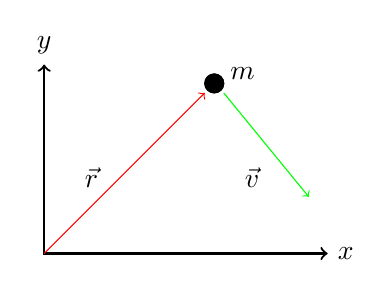
\begin{tikzpicture}[scale=1.2]
\draw [<->,thick] (0,2) node (yaxis) [above] {$y$}
        |- (3,0) node (xaxis) [right] {$x$};
\draw[->, red](0,0)--(1.7,1.7);
\filldraw[fill=black] (1.8,1.8) circle (0.1);
\draw (2.1,1.9) node (mass) {$m$};
\draw (.5,.8) node{$\vec{r}$};
\draw [fill=black] (1.8,1.8) circle(0.1);
\draw[->, green](1.9,1.7)--(2.8,0.6);
\draw (2.2,.8) node{$\vec{v}$};
\end{tikzpicture}
\end{marginfigure}


\bas
    \rmt{Linear Momentum: } & \vec{P} = m\vec{v}\\
    \rmt{Angular Momentum: } & \vec{L} =\vec{r}\times\vec{p}\\
    \rmt{Kinetic Energy: } & T  = \frac{1}{2}m v^2 = \frac{\abs{\vec{P}}^2}{2m}\\
    \rmt{Total Mechanical Energy: } & H  = T + V
\eas

The quantities, together with the position of the object, describe the classical \emph{state} of the system. The conservation laws corresponding to these quantities are also useful.
\marginnote[-2cm]{All three of these conservation laws are closely connected to symmetries, thanks to Noether's Theorem.  Conservation of Linear Momentum corresponds to a translational symmetry, Angular momentum corresponds to rotational symmetry, and conservation of energy corresponds to time translational symmetry.}
\bas
    \rmt{Conservation of Linear Momentum: } & \rmt{If } \sum{\vec{F}_\rmt{ext}}=0  \rmt{, then } \frac{d\vec{P}}{dt}=0\\
    \rmt{Conservation of Angular Momentum: } & \rmt{If } \sum{\vec{\tau}_\rmt{ext}}=0  \rmt{, then }\frac{d\vec{L}}{dt}=0\\
    \rmt{Conservation of Mechanical Energy: } & \rmt{If } \frac{\partial V}{\partial t}=0 \rmt{, then } \frac{dH}{dt}=0
\eas

\section{Electricity and Magnetism}

We will often be dealing with charged particles in our quantum systems, so it will be useful to have a handful of relationships from E\&M available to us.  First, we've got the basic electric field $\vec{E}$ at a position $\vec{r}$ due to a point charge $q_1$, which is:
\begin{marginfigure}[-1cm]
\centering
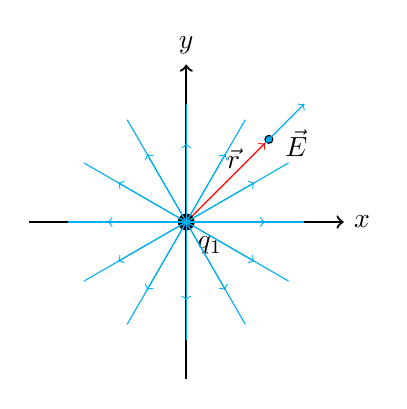
\begin{tikzpicture}[scale=1]
\draw [->,thick] (0,-2) -- (0,2) node (yaxis) [above] {$y$};
\draw [->,thick] (-2,0) -- (2,0) node (xaxis) [right] {$x$};

\draw (.3,-.3) node (charge) {$q_1$};
\draw (.6,.8) node{$\vec{r}$};
\draw[->,red](0,0) -- (1,1);
\filldraw[fill=black] (0,0) circle (0.1);

\filldraw[fill=cyan] (1.05,1.05) circle(0.05);
\draw[->,cyan](1,1)--(1.5,1.5);
\draw (1.4,1) node{$\vec{E}$};

\foreach \a in {0, 30,...,359}
    \draw[thin,cyan] (\a:0) -- (\a:1.5); 
\foreach \a in {0, 30,...,359}
    \draw[thin,cyan,->] (\a:0) -- (\a:1); 
    
\end{tikzpicture}
\end{marginfigure}
\beq
\vec{E} = \frac{1}{4\pi\epsilon_0}\frac{q_1}{r^2}\hat{r}.
\label{eq:efield}
\eeq

Then if we place a second charge $q_2$ near the first charge, we can find the electric potential energy $V$:
\begin{marginfigure}[-1cm]
\centering
\begin{tikzpicture}[scale=1.2]
\draw [<->,thick] (0,2) node (vaxis) [above] {$V$}
        |- (3,0) node (xaxis) [right] {$r$};
\draw[color=blue,domain=0.5:3] plot (\x,{1/(\x)}) node[right] {$V = \frac{1}{4\pi\epsilon_0}\frac{q_1q_2}{r}$};
\end{tikzpicture}
\end{marginfigure}

\beq
V = \frac{1}{4\pi\epsilon_0}\frac{q_1 q_2}{r}.
\eeq

We'll be using the dipole model for a number of different systems.  An electric dipole $\vec{p}_E$ is created when two charges of equal magnitude and opposite charge are separated by a distance $\vec{d}$,
\begin{marginfigure}
\centering
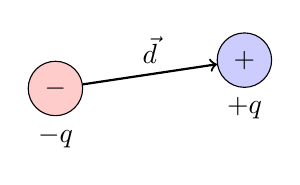
\begin{tikzpicture}[scale=1.2]
\path ( 0,0) node (q1) [shape=circle,draw,fill=red!20,label=below:$-q$] {$-$}
 ( 2,.3) node (q2) [shape=circle,draw,fill=blue!20,label=below:$+q$] {$+$};
 \draw [->,thick] (q1) -- (q2) node[above,midway]{$\vec{d}$};
\end{tikzpicture}
\end{marginfigure}
\beq
\vec{p}_E = q \vec{d}.
\eeq

Similarly, we can define the magnetic dipole $\vec{\mu}$ that is created when a current $I$ flows around a circle of area $A$ with normal vector $\hat{n}$,
\begin{marginfigure}
\centering
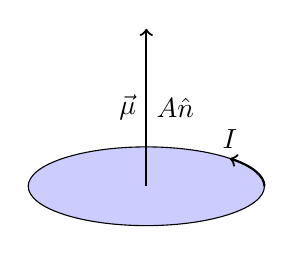
\begin{tikzpicture}[scale=1]
 \draw [fill=blue!20] (0,0) ellipse (1.5 and 0.5);
 \draw [->,thick] (0,0) -- (0,2) node[right,midway]{$A\hat{n}$} node[left,midway]{$\vec{\mu}$};
 \draw [->, thick] (1.5,0) arc (0:45:1.5 and 0.5) node[above]{$I$};
\end{tikzpicture}
\end{marginfigure}
\beq
\vec{\mu} = I A \hat{n}.
\eeq

When the magnetic dipole $\vec{\mu}$ is in an external magnetic field $\vec{B}$, there is a potential energy due to the interaction between the dipole and the field:
\begin{marginfigure}
\centering
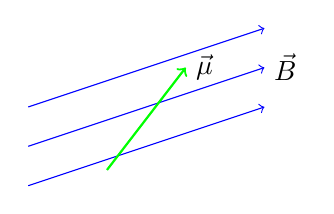
\begin{tikzpicture}[scale=1]
\draw[->,blue] (0,0) -- (3,1);
\draw[->,blue] (0,0.5) -- (3,1.5) node[right,black]{$\vec{B}$};
\draw[->,blue] (0,1) -- (3,2);
\draw[->,green,thick] (1,0.2) -- (2,1.5) node[right,black]{$\vec{\mu}$};

\end{tikzpicture}
\end{marginfigure}
\beq
V_\textrm{dip}= - \vec{\mu}\cdot\vec{B}.
\eeq

\begin{example}
\label{ex:orbitalmu}
What is the magetic moment for a single electron ``orbiting'' a single proton at the Bohr radius $a_0=(4\pi\epsilon_0\hbar^2)/(m_e e^2)$?

\model We'll model both the electron and the proton as point charges and point masses. We'll also model the electron as undergoing uniform circular motion without any losses (friction, radiation, etc.).

\vis We picture this as a circular orbit shown in Figure \ref{fig:exorbit}.
\begin{figure}
\centering
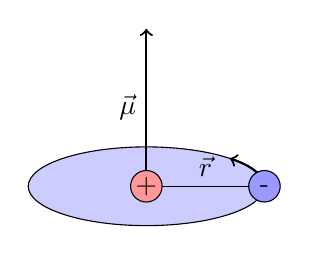
\begin{tikzpicture}
 \draw [fill=blue!20] (0,0) ellipse (1.5 and 0.5);
 \draw [->,thick] (0,0) -- (0,2) node[left,midway]{$\vec{\mu}$};
 
 \draw [->, thick] (1.5,0) arc (0:45:1.5 and 0.5);
 \draw (0,0) -- (1.5,0) node[midway,above] {$\vec{r}$};
 \draw[fill=blue!40] (1.5,0) circle (.2) node{-};
 \draw[fill=red!40] (0,0) circle (.2) node{+};
 
\end{tikzpicture}
\caption[][2cm]{ Circular electron ``orbit''.}
\label{fig:exorbit}
\end{figure}

\sol Since the distance between the proton and the electron stays constant, the area swept out by the electron is: $A = \pi a_0^2$. Since we are modeling the electron as going in uniform circular motion with a period $T$, the current is just $I = e/T$. We can use the uniform circular motion model along with the Coulomb force ($F = m_e v^2/a_0= eE$) to find the period of the motion, since, for uniform circular motion, the velocity is $v = (2\pi a_0)/T$. This means that 
\beq
\frac{e}{T}=\sqrt{\frac{1}{4\pi\epsilon_0}\frac{e^2}{a_0^2}\frac{e^2}{4\pi^2a_0m_e}}.
\eeq
So, the magnetic dipole moment is:
\beq
\mu=I A = \pi a_0^2 \frac{e}{T} = \frac{e \hbar}{2m_e}.
\eeq\arnote[-1.5cm]{Work through this to make sure you get the end step.}
Of course, you should run through this algebra in your notes and make sure you get the same answer. I mean it --- stop right now and do it!

\assess Checking our units, we expect to have units [m$^2$ C/s]. What we got has units: [C J$\cdot$s/kg] which is [C (kg$\cdot$m$^2$/s)/kg] which is what we want.

\end{example}


\begin{exercise}
What would the stored potential energy (in eV) of a charged system be if we held a single proton and a single electron apart the distance of the classical Bohr radius?

\end{exercise}


\section{Electromagnetic Waves}
\label{sec:elmaw1}
Of course we are going to need some mechanisms to describe the behavior of light. We'll start with a straight-forward description of a plain electromagnetic wave propagating along the $x$ axis.\marginnote{We use the term {\em electromagnetic wave} so much, we'll shorten it to {\em ElMaW}, pronounced like ``elmer'' with a softer end.} The wavelength is $\lambda$ and we define the wavenumber $k=2\pi/\lambda$.  Similarly, the wave has a time period of $T$ and an angular frequency $\omega = 2\pi/T$.  In this configuration we have coupled electric and magnetic fields:
\begin{marginfigure}
\centering
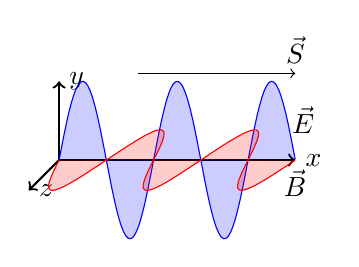
\begin{tikzpicture}[scale=1]
\draw[->,thick] (0,0,0) -- (3,0,0) node[right]{$x$};
\draw[->,thick] (0,0,0) -- (0,1,0) node[right]{$y$};
\draw[->,thick] (0,0,0) -- (0,0,1) node[right]{$z$};
\draw[color=blue,domain=0:3,fill=blue,samples=100, fill opacity=0.2] plot (\x,{sin(300*\x)},0) node[right,above,black,fill opacity=1,shift={(.1,.2,0)}] {$\vec{E}$};
\draw[color=red,domain=0:3,fill=red,samples=100, fill opacity=0.2] plot (\x,0,{sin(300*\x)}) node[right,below,black,fill opacity=1] {$\vec{B}$};
\draw[->](1,1.1,0) -- (3,1.1,0) node[above]{$\vec{S}$};
\end{tikzpicture}
\end{marginfigure}
\bas
E_y =& E_0 \sin(kx - \omega t)\\
B_z =& B_0 \sin(kx - \omega t).
\eas
For an electromagnetic wave moving through vacuum, the electric field and magnetic field amplitudes are related to each other such that $B_0 = E_0/c$, where $c$ is the speed of light, which, in turn, is also related to the electric field and magnetic field constants $\epsilon_0$ and $\mu_0$:
\beq
c^2 = \frac{1}{\mu_0\epsilon_0}.
\eeq
We need a couple of more things about electromagnetic waves. First, the Poynting vector $\vec{S}$ describes the movement of energy of the electromagnetic wave and can be written in terms of the electric and magnetic fields, pointing in the direction of propagation:
\beq
\vec{S}=\frac{1}{\mu_0}\vec{E}\times\vec{B} =c\epsilon_0 E_0^2 \hat{x} \sin^2(kx - \omega t).
\label{eq:poynting}
\eeq
We can now relate the energy transmission of the electromagnetic wave (per unit area) to the Poynting vector: 
\beq
I =\abs{\vec{S}_\rmt{avg}} = \frac{c\epsilon_0}{2}E_0^2.
\eeq

\begin{marginfigure}
\centering
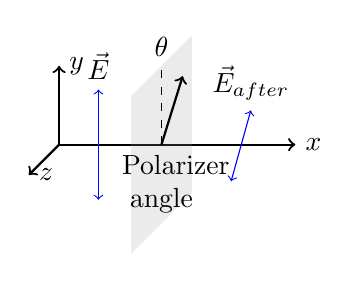
\begin{tikzpicture}[scale=1]
\draw[->,thick] (0,0,0) -- (3,0,0) node[right]{$x$};
\draw[->,thick] (0,0,0) -- (0,1,0) node[right]{$y$};
\draw[->,thick] (0,0,0) -- (0,0,1) node[right]{$z$};
\draw[color=blue,<->](.5,-.7,0) -- (.5,.7,0) node[above,black]{$\vec{E}$};
\fill[fill=black!40, fill opacity=0.2] (1.3,-1,-1)--(1.3,-1,1)--(1.3,1,1)--(1.3,1,-1)--cycle;
\draw[dashed](1.3,0,0) -- (1.3,1,0) node[above]{$\theta$};
\draw[->,thick](1.3,0,0) node[below,text width=1cm,align=center]{Polarizer angle}-- (1.3,.6,-.7) ;
\draw[color=blue,<->](2.3,-.35,.3) -- (2.3,.3,-.35) node[above,black]{$\vec{E}_\rmt{after}$};
\end{tikzpicture}
\end{marginfigure}
And, finally, we need to say something about the polarization of the wave. Because we are typically going to be working with a model that the interaction between the electromagnetic waves and matter will be dominated by the electric field, we define the polarization as the direction of the electric field vector. The effect of passing through a polarizer is to only pass the component of the electric field vector that points along the direction of the polarizer \ie $E_\rmt{final} = E_\rmt{initial} \cos\theta$, where $\theta$ is the angle between the polarizer and the incoming electric field vector. If we send randomly polarized light, the polarizer will pass half the initial intensity  and the output electric field will be polarized along the polarizer direction.

\begin{exercise}
A beam of unpolarized light from the sun with an initial intensity of 1000 W/m$^2$ passes through an initial polarizer, then through a second polarizer rotated by 45$^\circ$. What is the intensity and polarization of the output beam?
\end{exercise}


\subsection{Field Superposition}
We will frequently use the concept of superposition. The idea is that if we have two waves (or two electric fields, or two magnetic fields, etc.), we can find the total amplitude by adding up the amplitudes of the combined waves (or fields). In terms of the electric field, this means that the net (or total) electric field $\vec{E}_\rmt{total}$ at a point is a sum of all $N$ electric fields at that point:
\beq
\vec{E}_\rmt{total} = \sum_{i=1}^{N}\vec{E}_i
\eeq

\section{Waves}
\label{sec:waves}
A function that is propagating with some speed $v$ can be written in general as a right-moving wave (in the positive $x$ direction): $f(x - vt)$, or as a left-moving wave $f(x+vt)$. We saw this in the electromagnetic waves above for a sine wave, but it works in general for any function.

If we have two waves with the same amplitude along the same axis, but moving in opposite directions, it is the same as having a standing wave, i.e. a wave that oscillates up and down but does not move left or right.
\begin{example} What is the net wave if two traveling beams of light going opposite directions interfere in a region of space?

\model We model the two beams as electromagnetic waves with the same wavelength and frequency as the oscillations of their electric fields. 

\vis We have two waves approaching each other in Figure \ref{fig:wavesexample}.

\begin{figure}
\centering
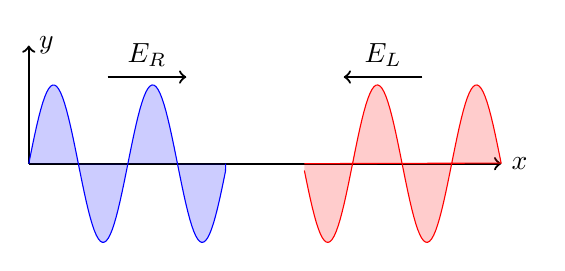
\begin{tikzpicture}
\draw[->,thick] (0,0) -- (6,0) node[right]{$x$};
\draw[->,thick] (0,0) -- (0,1.5) node[right]{$y$};
\draw[color=blue,domain=0:2.5,fill=blue,samples=100, fill opacity=0.2] (0,0) plot (\x,{sin(286*\x)}) -- (2.5,0)  ;
\draw[color=red,domain=3.5:6,fill=red,samples=100, fill opacity=0.2] (6,0) plot (\x,{sin(286*(6-\x)}) -- (3.5,0);
\draw[->,thick] (1,1.1) -- (2,1.1)node[midway,above,black,fill opacity=1] {$E_\rmt{R}$};
\draw[->,thick] (5,1.1) -- (4,1.1)node[midway,above,black,fill opacity=1] {$E_\rmt{L}$};
\end{tikzpicture}
\caption[][2cm]{ }
\label{fig:wavesexample}
\end{figure}

\sol Both waves are moving, one to the right and one to the left
\beq
E_\rmt{R}=E_0\cos(kx - \omega t)\ \rmt{and}\ E_\rmt{L}= E_0\cos(kx + \omega t)
\eeq
We find the sum of the two waves by applying the superposition principle: $E_\rmt{total}=E_\rmt{R}+E_\rmt{L}$. When we add these two waves, we re-write the trig functions such that we get a total wave amplitude of:
\beq
E_\rmt{total}=2E_0\cos kx \cos \omega t
\eeq
which is a standing wave as we expected. Of course, like usual, you need to go work out that trig work on your own.

\assess The maximum amplitude we get with this superposition is $2E_0$, which makes sense. The best way to assess this, though, is to animate it using your \CAS~and make sure it does what you want it to do. 

\end{example}
\arnote[-6cm]{Work through this to make sure you get the end step. Here's a hint: use a \texttt{TrigExpand} function on your favorite computer algebra system (\CAS) to get things rolling.}

\subsection{General Interference}
We can work with the superposition of any two waves by looking at the way in which the phases of the waves interact. We consider two electric field waves $E_1$ and $E_2$ that have the same wavelength and frequency but have a different phase offset $\phi_1$ and $\phi_2$:
\bas
E_1=&E_0\cos(kx-\omega t + \phi_1)\\
E_2=&E_0\cos(\underbrace{kx-\omega t + \phi_2}_{\rmt{Total wave phase}}).
\eas
We typically are looking for places where the waves add constructively or destructively. We will find constructive inference if the total phase of the sum of the waves $\Delta\phi$ is an integer multiple of $2\pi$. The interference will be destructive if the total phase is a half-integer multiple of $\pi$:
\beq 
\left.
\begin{aligned}
\rmt{Constructive: } & \Delta\phi = 2\pi n\\
\rmt{Destructive: } & \Delta\phi = 2\pi \left(n+\frac{1}{2}\right)
\end{aligned}
\right\}\  n=0,1,2,\ldots
\eeq
In one dimension, we model the total phase difference as the difference between the wave positions $\Delta x$ plus any initial phase offset $\Delta \phi$:
\arnote{Work through this to make sure you get the end step.}
\bas
\Delta\phi = & (kx_2 - \omega t + \phi_2) - (kx_1 - \omega t + \phi_1)\\
= & k\Delta x + \Delta\phi_\rmt{init}
\eas
where $\Delta x= x_2 - x_1$ and  $\Delta\phi_\rmt{init} = \phi_2-\phi_1$.

\subsection{Math Interlude: Complex Numbers}
We will be using complex numbers extensively. A complex number $z$ (and its complex conjugate $z^*$) can be written in terms of real numbers $x$, $y$, $r$, and $\theta$ in a number of different ways:
\bas
z &=x+\I y         & z^*&=x-\I y         & x &=r \cos\theta\\
 &=r\E{\I\theta} & &=r\E{-\I\theta}   & y &=r \sin\theta.
\eas

\section{Complex Electromagnetic Wave Amplitude Model (CEWAM)}
\label{sec:CEWAM}
It is really useful to model the electromagnetic waves using complex numbers. This will make it much easier for us to do calculations in a number of situations. The model (in one dimension) describes a traveling wave polarized in the $y$-direction as
\beq
E_y = E_0\E{\I(kx-\omega t)}.
\label{eq:CEWAM}
\eeq
When we want to connect back to the real electric field, we expand the exponential using the Euler formula and then take the real part.\marginnote{The Euler formula is:
\beq\E{\I\theta} = \cos\theta + \I\sin\theta.\eeq} The intensity of this wave is then calculated by taking the electric field times its complex conjugate:
\beq
I = \frac{c \epsilon_0}{2}E E^* = \frac{c \epsilon_0}{2}\abs{E}^2 = \frac{c \epsilon_0}{2}E_0^2,
\label{eq:CEWAMInt}
\eeq
where we have used the notation $EE^*$ = $\abs{E}^2$. Also note that when you multiply a complex number by its complex conjugate, the phase pieces multiply to give $1$: $\E{\I\theta}\E{-\I\theta}=\E{0}=1$.

\arnote[10cm]{As usual, work through this to make sure you get the end step. Look up the trig identities and how they relate to the complex exponential. Try using \texttt{ExpToTrig} with your favorite \CAS. }

\begin{example}
Use the CEWAM to find the interference intensity of two light beams that are slightly offset in one dimension.

\model We will model the two electromagnetic waves as moving in the same direction with the same frequency, wavelength and amplitude (which will stay constant) using the complex amplitude model. We'll model the beam offset as a $\Delta x$.

\vis The two waves are offset by just a bit, shown in Figure \ref{fig:excewam2}.

\begin{figure}
\centering
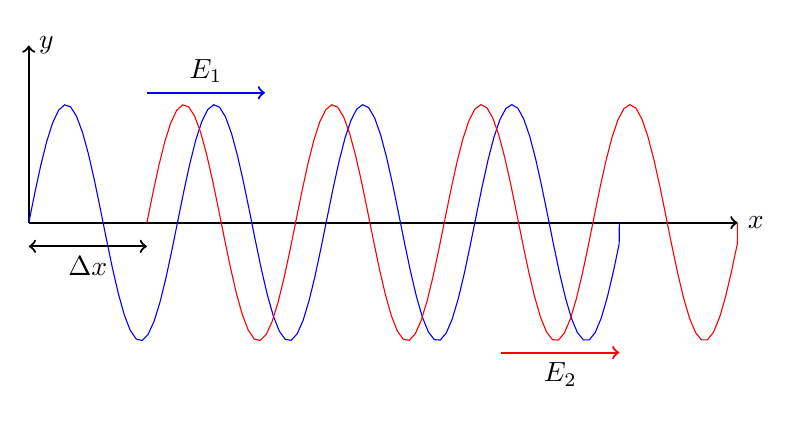
\begin{tikzpicture}[scale=1.5]
\draw[->,thick] (0,0) -- (6,0) node[right]{$x$};
\draw[->,thick] (0,0) -- (0,1.5) node[right]{$y$};
\draw[color=blue,domain=0:5,samples=100] (0,0) plot (\x,{sin(286*\x)}) -- (5,0)  ;
\draw[color=red,domain=1:6,samples=100] (1,0) plot (\x,{sin(286*(\x-1)}) -- (6,0);
\draw[->,thick,blue] (1,1.1) -- (2,1.1)node[midway,above,black,fill opacity=1] {$E_1$};
\draw[->,thick,red] (4,-1.1) -- (5,-1.1)node[midway,below,black,fill opacity=1] {$E_2$};
\draw[<->,thick](0,-.2) -- (1,-.2) node[midway,below]{$\Delta x$};
\end{tikzpicture}
\caption[][2cm]{ }
\label{fig:excewam2}
\end{figure}

\sol Since we are interested in the intensity (the one thing we can easily measure), we need to find the net electric field amplitude and then use Eq.~(\ref{eq:CEWAMInt}) to find the intensity of the combined beams.
\bas
E_1 &=  E_0 \E{\I(k x_1 -\omega t)}\\
E_2 &=  E_0 \E{\I(k x_2 -\omega t)}.
\eas
The net electric field is then $E_\rmt{total} =E_1 + E_2$. We just add these together and then find the intensity:
\bas
I=& \frac{c \epsilon_0}{2}E_\rmt{total} E_\rmt{total}^*\\
=&\frac{c \epsilon_0}{2}\left(\abs{E_1}^2+\abs{E_2}^2 + E_1^*E_2 + E_1 E_2^*\right)\\
=&\frac{c \epsilon_0}{2}\left(2E_0^2 + E_0^2\left(\E{\I(k x_2-k x_1)}\right) + E_0^2\left(\E{\I(k x_1-k x_2)}\right)\right)\\
=&\frac{c \epsilon_0}{2}E_0^2\left(2 + 2 \cos(k\Delta x) \right).
\eas
So the intensity could be anywhere from a maximum of $2c\epsilon_0 E_0^2$ if $k\Delta x = 0, 2\pi, 4\pi, \ldots$ to a minimum of zero if $k \Delta x = \pi, 3\pi, \ldots$. 

\assess The limits look right for the max and the min: a max happens when $\Delta x = 2 \pi/k = \lambda$, which makes sense. The minima happened when $\Delta x = \lambda/2$.

\end{example}

\begin{exercise}
Use the CEWAM to find the interference of two point-source waves (i.e. the double-slit interference model) on a screen a long distance away from the sources. I encourage you to go back to your notes from previous classes to see how you did this before and then do it again with this new model.
\end{exercise}

\begin{exercise}
Describe the motion and behavior of a polarized wave with the following components:
\bas
E_y =& E_0 \E{\I(kx -\omega t)}\\
E_z =& E_0 \E{\I(kx -\omega t + \pi/2)}.\\
\eas

\end{exercise}

%----------------------------------------------------------------------------------------
% Chapter 2
%----------------------------------------------------------------------------------------
\chapter{Creating Electromagnetic Waves}

Ok, this really is a guidebook for a quantum mechanic. And we really will get to doing some work under the hood, so to speak, with our quantum tools. However, I want to motivate the need for a new set of models to describe the quantum world. So we look for places or situations where our current models don't seem to work any more. One of those is in the uniform circular motion model of the electron orbiting around the proton. We've used the model a number of times, but there is a real problem with it. To get at that problem, we need to build of model of electromagnetic wave generation.

\section{Classically Accelerated Charges}
We introduced, back in introductory physics, the idea that an accelerating charge can generate an electromagnetic wave. We used a simple model where we have an oscillating current moving up and down a long center-fed wire.
\begin{marginfigure}\centering
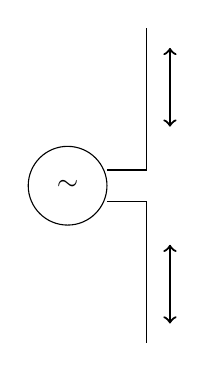
\begin{tikzpicture}[scale=1]
\draw (0,0) circle (.5) node(source){$\sim$};
\draw(.5,.2) -- (1,.2) -- (1,2);
\draw(.5,-.2) -- (1,-.2) -- (1,-2);
\draw[<->,thick](1.3,.75) -- (1.3,1.75);
\draw[<->,thick](1.3,-.75) -- (1.3,-1.75);
\end{tikzpicture}
\end{marginfigure}

As the electrons accelerate up and down, the electric and magnetic fields they produce begin to look like electromagnetic waves. We will build a simple model for how an accelerating electric charge can generate electromagnetic waves.
\subsection{Larmor Radiation}
\marginnote{We're following Purcell's derivation here.}
Here's the model: a single electron is traveling at a constant speed $v$. After some time $T$, the electron abruptly decelerates to rest (for a total change in velocity of $\Delta v$) over a short time interval $\Delta T$. If we look at the electric field lines that could come from the charge, we would get something that looks like the figure on the right. However, the electric field lines must have smoothly shifted from the one position to the other, so we will focus in on how they make that transition.

\begin{marginfigure}\centering
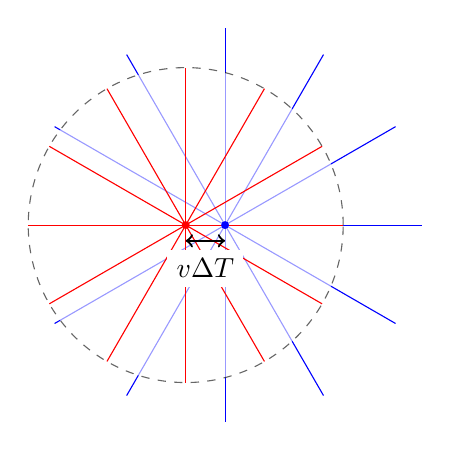
\begin{tikzpicture}[scale=1]
  \begin{scope}[shift={(0.5,0)}]
    \foreach \a in {0, 30,...,359}
    \draw [blue](\a:0) -- (\a:2.5); 
  \end{scope}
\filldraw[dashed, fill=white, opacity=0.6] (0,0) circle (2);
\foreach \a in {0, 30,...,359}
    \draw [red] (\a:0) -- (\a:2); 
\draw[<->,thick] (0,-.2) -- (0.5,-.2) node[fill=white,below,midway,shift={(0,-.1)}]{$v \Delta T$};
\fill[red] (0,0)circle(0.05);
\fill[blue] (.5,0) circle(0.05);
\end{tikzpicture}
\end{marginfigure}

Zooming in on one line, we have the following, where we have expanded the short deceleration interval $\Delta T$ which is much faster than the time $T$.  The blue point is where the charge {\em would have been} if it hadn't stopped. In particular, we are interested in the radial and transverse components of the electric field $E_r$ and $E_t$ during the acceleration interval. We assume that the signal of the acceleration travels outward at the speed of light. At some time $T$ later, the signal has traveled $r=cT$ as depicted in Figure \ref{fig:larmor}.

\begin{figure}
\centering
\begin{tikzpicture}[scale=2]

\fill[fill=blue!20] (2,0) -- (2.5,0) arc(0:60:2.5) -- (60:2) -- (60:2) arc(60:0:2);
\draw[dashed] (2,0) arc (0:60:2);
\draw[dashed] (2.5,0) arc (0:60:2.5);
\draw[<->] (50:2) -- (50:2.5) node[above,shift={(.4,0)}]{$c\Delta T$};
\draw[<->,thick] (-.5,-.2) -- (0,-.2) node[below,midway,shift={(0,-.1)}]{$v T$};
\fill[blue] (0,0)circle(0.05);
\fill[red] (-.5,0) circle(0.05);
\begin{scope}[shift={(-0.5,0)}]
    \draw[thick](30:0) coordinate(pt4) -- (30:2.43) coordinate(pt2) node[midway,above,shift={(-.5,0)}]{$r=cT$};
\end{scope}

\draw[thick] (-1,0) -- (3,0);
\draw[dashed](1,0) arc (0:30:1) node[midway,right]{$\theta$};

\draw[dashed] (30:0) coordinate(pt0) -- (30:2.5) coordinate(pt1);
\draw[thick] (pt2) -- (pt1);
\draw[thick] (30:2.5) -- (30:2.95);
\draw[<->,red] (30:2) coordinate(pt3) -- (30:2.5) node[midway,below]{$E_r$};
\draw[<->,red] (pt2)--(pt3) node[midway,left,shift={(0,-0.2)}]{$E_t$};
\draw[dashed] ($(pt4)!(pt0)!(pt2)$) -- (pt0) node[midway,right,rotate=30] {$v T \sin\theta$};
\end{tikzpicture}
\caption[][2cm]{The electric field lines are offset by the accelerated charge.}
\label{fig:larmor}
\end{figure}

We now look at the ratio of the two electric field components $E_t/E_r$ which is unitless:
\beq
\frac{E_t}{E_r} = \frac{v T \sin\theta}{c\Delta T}.
\eeq

But the radial electric field in just given by Eq.~(\ref{eq:efield}), so we have:
\beq
E_t = \frac{q}{4\pi\epsilon_0 r^2} \frac{(v/\Delta T) (cT)}{c^2}\sin\theta.
\label{eq:etprelarmor}
\eeq
Since $v/\Delta T$ is the acceleration $\dot{v}$ and the radius $r = cT$, we simplify this to:
\arnote{Make sure you can get here in your notes.}
\beq
E_t = \frac{q}{4\pi\epsilon_0 r^2} \frac{\dot{v}r}{c^2}\sin\theta.
\eeq
The outgoing energy transmission per unit area of this transverse electric field is given by the Poynting vector, Eq.~(\ref{eq:poynting}), $S =c\epsilon_0E_t^2$. This means that the total energy loss $dU/dt$ must be integrated over the whole sphere of radius $r$:
\beq
\frac{dU}{dt} = \int_{0}^{2\pi}\int_{0}^{\pi} S\ r^2 \sin\theta d\theta d\phi.
\label{eq:dudtprelarmor}
\eeq
Use your favorite \CAS to do this integral and you should get the rate of energy loss by an accelerating charge as:
\beq
\frac{dU}{dt} = \frac{q^2\dot{v}^2}{6\pi c^3\epsilon_0}
\label{eq:larmor}
\eeq\marginnote[-1.5cm]{You will work this out as an exercise.}
which is known as the Larmor radiation formula.
\begin{exercise}
Work through the steps needed to get from Eq.~(\ref{eq:etprelarmor}) to Eq.~(\ref{eq:larmor}). Be sure to include your model, visualization, and assessment (\ie check that the units work out).
\end{exercise}



\section{Hydrogen Radiation Problem}
We now have everything we need to re-visit the model of an electron in uniform circular motion about a stationary proton. The radial acceleration (from $F_r = m a_r$) of the electron is
\begin{marginfigure}\centering
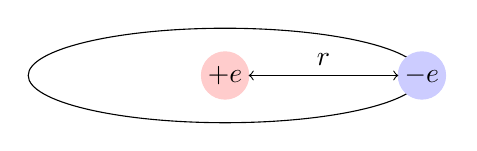
\begin{tikzpicture}[scale=1]
\draw (0,0) ellipse(2.5 and .6);

\filldraw[red!20] (0,0)circle(0.3) node[black]{$+e$};
\filldraw[blue!20] (2.5,0) circle(0.3) node[black]{$-e$};
\draw[<->](.3,0) -- (2.2,0)node[above,midway]{$r$};

\end{tikzpicture}
\end{marginfigure}
\beq
a_r = \dot{v} = \frac{1}{m_e}\frac{e^2}{4\pi\epsilon_0r^2}.
\eeq

We'll model the electron as it orbits the proton at a distance of $a_0$, the Bohr radius we used in Example \ref{ex:orbitalmu}. But, as we just saw with the Larmor formula, any charged particle undergoing accelerations emits radiation. The energy emitted must come from somewhere --- and in this case, it must be from the mechanical energy of the orbit. We need the total mechanical energy for an object undergoing uniform circular motion. We know the potential and kinetic energies. We use the fact that we are going in circular motion to simplify the total energy to $U = -e^2/(4\pi\epsilon_0 (2r))$. \arnote{There are a bunch of steps I skipped in here. Go through them and be explicit on each step so that you get this same result.} We take the time derivative of this to get
\beq
\frac{dU}{dt}=\frac{e^2}{4\pi\epsilon_0}\frac{\dot{r}}{2r^2}.
\label{eq:energyderivative}
\eeq
We want how the radius changes with time (with an initial radius of $a_0$). So we equate this with Eq.~(\ref{eq:larmor}) to get a differential equation: \arnote{I skipped steps here, too. Work through them on your own.}
\beq
\dot{r}r^2 = -\frac{e^4}{12\pi^2\epsilon_0^2 c^3 m_e^2}.
\label{eq:rrdot}
\eeq
It helps some if we define a new length scale: $r_e = e^2/(4\pi\epsilon_0 c^2 m_e)$. We can then write the differential equation as:
\beq
\dot{r}r^2=-\frac{4}{3}r_e^2 c,
\eeq
which has a straight-forward solution with the initial condition that $r=a_0$ at $t=0$: \arnote{Three in a row-- work these out, too.}
\beq
r^3 = a_0^3-4 r_e^2 c t.
\label{eq:orbitdecay}
\eeq

Here's the problem with this model: Eq.~(\ref{eq:orbitdecay}) predicts that the orbit of the electron will start at $a_0$ and quickly decay to zero as seen in the figure! Furthermore, we don't measure this type of radiation coming from the hydrogen atom. So this model doesn't work. Similarly, no model where the electron is moving in any kind of classical orbit around the proton will work - they will all have this same problem. So we need a new model where the electron stays bound to the proton, but not in a classical orbit. \begin{marginfigure}\centering
\begin{tikzpicture}[scale=1]
\draw[->,thick] (0,0) node[left]{0} -- (4,0) node[right]{$t$};
\draw[->,thick] (0,0) node[below]{0}-- (0,3) node[right]{$r$};
\draw[color=blue,domain=0:3,samples=100] plot (\x,{(2^3-(2^3/3)*\x)^(1/3)});
\draw (0,2) node[left]{$a_0$};
\end{tikzpicture}
\end{marginfigure}

\section{Bohr Model}
\label{sec:bohr}
We have another piece of data that also points to the need for a new model. If the electron could classically orbit the proton, it should be able to orbit it at any radius. As the electron moved from one radius (total mechanical energy) to another (new total energy), there should be some kind of energy absorption or emission corresponding to this change in internal energy. If the electron can occupy any orbit, we would expect a continuous spectrum of energy emission. We measure energy emission from the hydrogen atom, but it isn't continuous.
\begin{marginfigure}\centering
\includegraphics[width=\textwidth]{Balmer.png}
\caption{From \href{http://chemwiki.ucdavis.edu/Textbook_Maps/General_Chemistry_Textbook_Maps/Map\%3A_Lower's_Chem1/04._Atoms_and_the_Periodic_Table/The_Bohr_Atom}{\texttt{chemwiki.ucdavis.edu/
Textbook\_Maps/General\_Chemistry
\_Textbook\_Maps/Map\%3A\_Lower's
\_Chem1/04.\_Atoms\_and\_the
\_Periodic\_Table/The\_Bohr\_Atom}}
}
\end{marginfigure}
There is a pattern to the emission lines if we make two assumptions: first, that the electron can only exist in specific energy configurations. We won't say anything more specific about these yet, but we can empirically note that the energy associated with each of the configurations is
\beq
E_n = -\frac{R_\infty h c}{n^2}
\eeq
where $R_\infty$ is a constant with units 1/length, $c$ is the speed of light, $h$ is Planck's constant, and $n$ is a positive integer. The second assumption is that the energy associated with the emitted light is inversely proportional to its wavelength with constant of proportionality $hc$ (where $c$ is the speed of light and $h$ is Planck's constant):
\beq
E = \frac{h c}{\lambda}.
\eeq
Put those two together and we see that the emitted wavelengths as the electron jumps from one configuration to another (like from $n_1$ to $n_2$) is
\beq
\frac{1}{\lambda} = \abs{R_\infty\left(\frac{1}{n_2^2} -\frac{1}{n_1^2}\right)}.
\eeq\marginnote{The \href{http://physics.nist.gov/cgi-bin/cuu/Value?ryd|search_for=rydberg}{numerical value of $R_\infty$} is $10973731.6$~m$^{-1}$.}%
Of course, there is more to this than the simple empirical relationship. However, this is enough for us for now. Each time the electron in an atom jumps from one allowed energy configuration to another it either absorbs energy from an electromagnetic wave (if it increases energy) or emits an electromagnetic wave (if it decreases in energy).

\begin{exercise}
\begin{enumerate}
\item There are a couple of named sequences of emission lines from the hydrogen atom. The second of these is the Balmer series which ends at a final energy configuration where $n_f = 2$. Calculate the first 6 possible wavelengths of transitions from higher energy states to this final state, plus the energy to go from $n=\infty$ to this state. Show your work (I don't really care if you can look up the answer on the internet. If I really needed you to give me the answer, I'd have done it myself. The point is to give you practice doing calculations!)

\item Do the same thing for the Bohr series where $n_f = 3$. Calculate the first 6 possible wavelengths of transitions from higher energy states to this final state, plus the energy to go from $n=\infty$ to this state. Show your work.
\end{enumerate}
\end{exercise}

\section{Detecting Electromagnetic Waves}

The last thing we need to do to get to a place where we explore quantum states is to build a model for detecting electromagnetic waves. We're almost there. Let's review what we know about electromagnetic waves (ElMaWs) and how we could detect them.

\begin{enumerate}
\item ElMaWs can make charges in matter accelerate. If we could connect a very fast ammeter to some kind of metal antenna, we could detect the wave. That works well for radio waves, but by the time we get to the visible wavelengths, the wave oscillations are too fast to measure.
\item ElMaWs carry energy. The intensity of a wave is a measure of power/area which is energy/(time$\cdot$area). So the energy deposited by an ElMaW could be detected and used.
\item We could measure the change in temperature as the energy from the ElMaW deposits its energy in a material. This works well, but tends to be slow - materials take time to heat up and respond thermally.
\item What if the incomming ElMaW has a wavelength less than $1/R_\infty$? Following our model from the last chapter, this corresponds to a transition going from $n=1$ to $n=\infty$. What does that mean? Experimentally, it means that the electron has climbed out of the potential well and is no longer bound to the proton - it has become a free electron! All we have to do now is detect that electron and we're home free!
\item The incoming ElMaW could cause a chemical change in a molecule. We could use chemistry to isolate the molecules that have undergone the chemical change and thus detect where the ElMaW was. This is how photopaper works.
\item Finally, we could use a semiconductor where there is an energy gap between an insulator state and a conductor state. If the incoming ElMaW has more energy than the size of the gap, it can deposit its energy, creating a current. We can then detect that current using an ammeter. This is how photovoltaics work.

\end{enumerate}

\subsection{Electron Detection}

There are a couple of ways we can detect a single free electron. One way is to use a series of positively charged plates to amplify the electron signal to a point where it can be detected. This is basically the way a photomultiplier works (PMT).  A microchannel plate (MCP) works in about the same way. So we have the tools we need to detect single free electrons, though in the detection of the electrons, they are essentially lost (\ie we smash them into other things so that they rebound in an uncontrolled, or mostly uncontrolled fashion).

This model gives us a way of reliably detecting ElMaWs using a hydrogen atom as long as the ElMaW has a wavelength less than $1/R_\infty$. Or if the hydrogen atom starts in a different configuration, we could detect the wave if $\lambda < n_\rmt{initial}/R_\infty$.

But this model doesn't work very well in practice. It is hard to work with and fairly restrictive. What if we could use something more solid as an ElMaW detector? The photoelectric effect model describes exactly that. Metals behave similarly to our simple hydrogen model in that we can quantify a ``work function'' $\Phi$ in energy units that describes how much energy is required to pop an electron off of the surface. If the incoming ElMaW has a wavelength less than $\lambda < h c/\Phi$, the ElMaW could pop an electron.  \marginnote{However, this model doesn't take into the many complications such as the possibility of the incoming ElMaW deponsiting its energy in thermal energy. Or accelerating the electron in the surface without popping it off. Typically a PMT is only about 20\% effective at converting ElMaWs to electrons.}

\begin{exercise}
There is a list of work functions given at:
\begin{center}
\href{http://hyperphysics.phy-astr.gsu.edu/hbase/tables/photoelec.html}{
\texttt{http://hyperphysics.phy-astr.gsu.edu/hbase/tables/
photoelec.html}.}
\end{center}
Compile a list of metals that would be suitable for detecting light with wavelength $\lambda = 532$~nm. Again, be explicit with your model, visualization, and assessment.
\end{exercise}

What we are looking for is a detector that reacts very fast and has precise timing. The PMT and the MCP both fit the bill, so we will model our detectors as one of them. We will visualize our detection scheme like Figure \ref{fig:detectorschematic}.
\begin{figure}
\centering
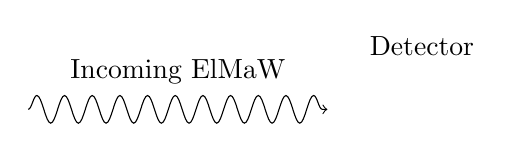
\begin{tikzpicture}
\draw[->,decorate, decoration={snake,amplitude=5,segment length=10}](0,0)--(3.8,0) node[midway,above,shift=({0,.2cm})]{Incoming ElMaW};
\detector{1}{4}{0}{0}
\node[] at (5,0.8) {Detector};
\end{tikzpicture}
\caption[][2cm]{ }
\label{fig:detectorschematic}
\end{figure}

We connect a fast oscilloscope to the detector and measure the output of the amplified electron signal. This gives us timing as to when the ElMaW kicked an electron off of the metal at the front of the detector. We might expect a signal something like Figure \ref{fig:detectorsignal} where each blip corresponds to an electron ionization event. However, when we turn up the intensity of the incoming ElMaW, we find that the signals start to overlap and eventually build up to a single, steady signal.
\begin{figure}
\centering
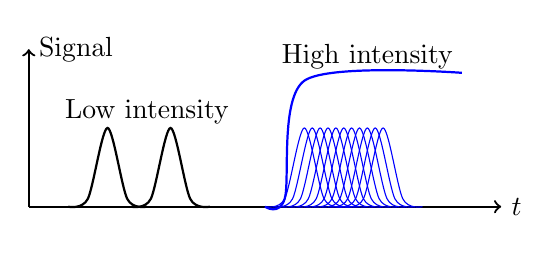
\begin{tikzpicture}
\draw[->,thick] (0,0) -- (6,0) node[right]{$t$};
\draw[->,thick] (0,0) -- (0,2) node[right]{Signal};
\draw[thick] plot[smooth] coordinates{(0.5,0)(.75,.1)(1,1)(1.25,.1)(1.5,0)};
\draw[thick,shift=({.8,0})] plot[smooth] coordinates{(0.5,0)(.75,.1)(1,1)(1.25,.1)(1.5,0)};
\draw (1.5,1.2) node{Low intensity};
\draw[thick,blue] plot[smooth] coordinates{(3,0)(3.25,.1)(3.5,1.6)(5.5,1.7)};

\foreach \a in {2.5,2.6,2.7,...,3.5}
    \draw[thin,blue,shift=({\a,0})] plot[smooth] coordinates{(0.5,0)(.75,.1)(1,1)(1.25,.1)(1.5,0)};

\draw (4.3,1.9) node{High intensity};

\end{tikzpicture}
\caption[][2cm]{ }
\label{fig:detectorsignal}
\end{figure}

\begin{example}
\label{ex:twogauss}
Model the amplified electron signal from the detector as a Gaussian pulse on the oscilloscope. What would the signal look like if two electrons arrived within the Gaussian width?
\model We will model the detector as an amplified electron coming from a metal where the electron was ejected from the surface by an ElMaW. We assume that every pulse is identical and only differs by its peak time. We model the peaks as the function: $\exp[-(t-t_k)^2/(2\sigma^2)]$ where $t_k$ is the arrival time of the $k$th pulse and $\sigma$ is the width of the pulse.

\vis The pulses will look like Figure \ref{fig:twogaussfig}.
\begin{figure}
\centering
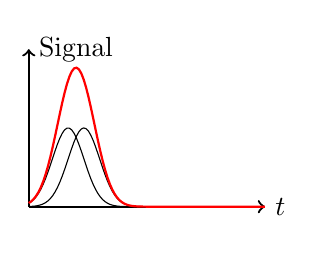
\begin{tikzpicture}
\draw[->,thick] (0,0) -- (3,0) node[right]{$t$};
\draw[->,thick] (0,0) -- (0,2) node[right]{Signal};

\draw[domain=0:3,samples=100] plot({\x},{exp(-(\x-.5)^2/(2*0.2^2))});
\draw[domain=0:3,samples=100] plot({\x},{exp(-(\x-.7)^2/(2*0.2^2))});

\draw[domain=0:3,samples=100,red,thick] plot({\x},{exp(-(\x-.7)^2/(2*0.2^2))+exp(-(\x-.5)^2/(2*0.2^2))});

\end{tikzpicture}
\caption[][2cm]{ }
\label{fig:twogaussfig}
\end{figure}

\sol We add up two Gaussians, modeling the functions as having a width of 0.2 and separated by 0.2.
\beq
\rmt{Sig}= \exp[-(t-0.5)^2/(2(0.2^2)] + \exp[-(t-0.7)^2/(2(0.2^2)]
\eeq
\assess The total signal is about twice the height and twice the width of a single pulse. That makes sense.
\end{example}

There is one more piece to this ideal detector model: we are going to ignore ``dark counts''. There are times when the detector will eject an electron even when there is no incoming ElMaW due to the thermal energy present in all objects not at absolute zero temperature. We can make this a very small effect, though, by cooling the detector. All together, we will call this the {\em ideal detector model}.\marginnote[-2cm]{A simple model for the emission of electrons is to model a ``thermionic current'' which is proportional to $T^2\E{-\Phi/kT}$ where $T$ is the detector temperature and $k$ is Boltzmann's constant.}


\begin{exercise}
What if we used a thermal detector? What would the change in temperature be if we directed an ElMaW with an intensity of 1000~W/m$^2$ on one face of an aluminum cube that is 10~cm on a side for one hour?
\end{exercise}


\chapter{Quantized Electromagnetic Waves}
Now we have most of the tools we need to explore the need for a quantum model. The one piece we are missing is a model of a beamsplitter. 
\section{Beamsplitters}
\label{sec:EMbeamsplitter}
The idea of a beamsplitter is to partially reflect and partially transmit an ElMaW. This can be accomplished with a partially silvered mirror, but they are usually made with thin film coatings so that they are less lossy.
\begin{marginfigure}\centering
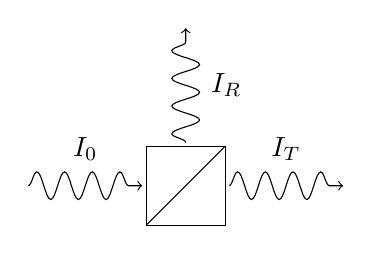
\begin{tikzpicture}
\draw (-0.5,-.5) rectangle +(1,1);
\draw (-.5,-.5) -- (.5,.5);
\draw[->,decorate, decoration={snake,amplitude=5,segment length=10, post length=.1cm}](-2,0)--(-.55,0) node[midway, above,shift=({0,.2cm})]{$I_0$};
\draw[->,decorate, decoration={snake,amplitude=5,segment length=10, post length=.1cm}](.55,0)--(2,0) node[midway, above,shift=({0,.2cm})]{$I_T$};
\draw[->,decorate, decoration={snake,amplitude=5,segment length=10, post length=.1cm}](0,.55)--(0,2) node[midway, right,shift=({.2cm,0})]{$I_R$};
\end{tikzpicture}
\end{marginfigure}
We will model our beamsplitter as having no losses and with a coating such that $I_R = I_T = I_0/2$, also known as a 50-50 beamsplitter. One of the aspects of energy conservation is that $I_R + I_T = I_0$, so we are good there.
How do we model the beamsplitter using the Complex Electromagnetic Wave Amplitude Model? We know that (Eq.~ (\ref{eq:CEWAMInt})) $I_0 = c\epsilon_0/2\abs{E_0}^2$. But this same relationship holds for $I_R = c\epsilon_0/2\abs{E_R}^2$. Relating these two, we find that
\bas
E_R = &\frac{E_0}{\sqrt{2}} \E{\I\phi_R}\;\;\rmt{and}\\
E_T = &\frac{E_0}{\sqrt{2}} \E{\I\phi_T},
\eas
where we have two arbitrary complex phases $\phi_R$ and $\phi_T$. But we also know that ElMaWs pick up a phase shift of $\pi$ on reflection, so $\phi_R - \phi_T = \pi$. To simplify our calculations, we can set $\phi_T=0$, so $\phi_R = \pi$.

\begin{example}
What are the electric field amplitudes for a 60-40 beamsplitter?

\model We model the beamsplitter as having no losses with a $\pi$ phase shift on the reflected beam. We let the 60\% arm be the reflected arm.

\vis The beamsplitter is shown in Figure \ref{fig:bsexampleprob}.

\begin{figure}
\centering
\begin{tikzpicture}
\draw (-0.5,-.5) rectangle +(1,1);
\draw (-.5,-.5) -- (.5,.5);
\draw[->,decorate, decoration={snake,amplitude=5,segment length=10, post length=.1cm}](-2,0)--(-.55,0) node[midway, above,shift=({0,.2cm})]{$I_0$};
\draw[->,decorate, decoration={snake,amplitude=5,segment length=10, post length=.1cm}](.55,0)--(2,0) node[midway, above,shift=({0,.2cm})]{$I_T = 0.4I_0$};
\draw[->,decorate, decoration={snake,amplitude=5,segment length=10, post length=.1cm}](0,.55)--(0,2) node[midway, right,shift=({.2cm,0})]{$I_R=0.6I_0$};
\caption[][2cm]{ }
\label{fig:bsexampleprob}
\end{tikzpicture}
\end{figure}

\sol So we have $I_R = 0.6 I_0$. Therefore $E_R = \sqrt{0.6}E_0 \E{\I\pi}$ and $E_T = \sqrt{0.4}E_0$.
\arnote{Make sure you work through these! I want to see your work.}

\assess When we square the amplitudes and add them, we end up back at $I_0$, so we've conserved energy. That's a good thing!

\end{example}
\begin{exercise}
What are the electric field amplitudes for beamsplitter with transmission $\alpha$ and reflection $(1-\alpha)$?
\end{exercise}

\subsection{Second-order Correlation}
\label{sec:correlation}
We split up a measurement of the output of our beamsplitter into time intervals $\Delta T$ and measure for a total time $T$. We now look at the relationship between the measured intensities of the two beams coming out of the beamsplitter and how they change (if at all) over time. This relationship, called the second-order correlation $g^{(2)}$, tells us how the two beams are related (or correlated). We are interested in the correlation between the two intensities at the same moment in time which is calculated by averaging over the time interval from $0$ to $\Delta T$ (denoted by $\avg{\;}$):
\beq
g^{(2)} = \frac{\avg{I_R(t) I_T(t)}}{\avg{I_R(t)}\avg{I_T(t)}}.
\label{eq:gtwo}
\eeq
We will use this second-order correlation to describe what is happening in our experiment setup below.

\begin{example}
What is $g^{(2)}$ if we measure a constant, equal intensity on the output of a 50-50 beamsplitter?

\model We model the beamsplitter as ideal and model the intensity as constant so that $I_R= I_T=I_0/2$. We want the second-order correlation.

\vis Constant intensities give us an intensity-versus-time graph that looks like Figure \ref{fig:constintensity}.
\begin{figure}
\centering
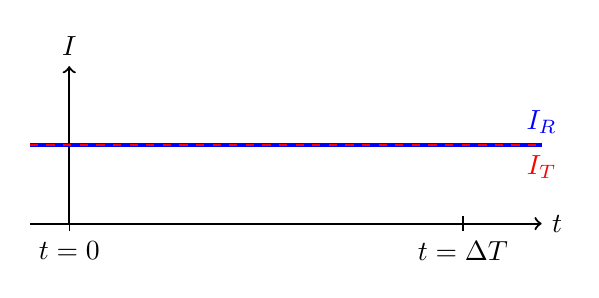
\begin{tikzpicture}[scale=1]
\draw[->,thick] (-.5,0) -- (6,0) node[right]{$t$};
\draw[->,thick] (0,0) -- (0,2) node[above]{$I$};
\draw(0,-.1) node[below] {$t=0$} -- (0,.1);
\draw(5,-.1) node[below] {$t=\Delta T$} -- (5,.1);
\draw[blue,ultra thick] (-.5,1) -- (6,1) node[above]{$I_R$};
\draw[dashed, red, thick] (-.5,1) -- (6,1) node[below]{$I_T$};

\end{tikzpicture}
\caption[][2cm]{ }
\label{fig:constintensity}
\end{figure}

\sol The average intensity over the interval is
\beq
\avg{I_R(t)} = \frac{1}{\Delta T} \int_0^{\Delta T} I_R(t) dt.
\eeq
and the same for the other average. Since both of these are constant, they are both just $I_R = I_0/2$ and $I_T=I_0/2$. Same thing with the average of the product:
\beq
\avg{I_R(t)I_T(t)} = \frac{1}{\Delta T} \int_0^{\Delta T} I_R(t)I_T(t) dt.
\eeq
So, the second-order correlation is just $g^{(2)} = 1$.\arnote{Be sure you work this through on your own from Eq.~(\ref{eq:gtwo}).}

\assess Ok, this gives us a baseline idea of what to expect for $g^{(2)}$.

\end{example}

\begin{exercise}
What is the second-order correlation for a short, gaussian-shaped pulse (like the one from Example~\ref{ex:twogauss} where the width is $0.2$ nanoseconds and the peak happens at $2.5$~ns) that is split by a 50-50 beamsplitter over a time interval of $t=0$~ns to $t=5$~ns?
\end{exercise}

We can do the same thing if we break up our time measurement into bins and measure the intensity in each bin. Then the averaging becomes a simple sum (divided by the number of bins).

\begin{exercise}
What is the second-order correlation at for the block of discrete bins shown in Table \ref{tab:normaltab}, where each bin is $100$~ns long and the intensities are all measured terms of the number of (distinct) electrons measured during the bin?
\begin{table}
\centering
\begin{tabular}{|c||c|c|c|c|c|c|c|c|c|c|c|c|}
\hline
$I_R$ & 4 & 5 & 4 & 6 & 8 & 5 & 9 & 4 & 6 & 9 & 7 & 5 \\ 
\hline
$I_T$ & 4 & 5 & 4 & 6 & 8 & 5 & 9 & 4 & 6 & 9 & 7 & 5\\
\hline
\end{tabular}
\caption[][1cm]{ }
\label{tab:normaltab}
\end{table}

\end{exercise}

\section{Coincidence Measurements}
\label{sec:coincid}
Ok. We are now ready to get at the heart of the quantum mechanic's guide. We are going to set up an experiment where we put a single trapped atom in a place where we can collect the electromagnetic waves that it emits. We will take those waves and direct them to a 50-50 beamsplitter and then put two identical detectors at the outputs of the beamsplitter.

\begin{figure}
\centering
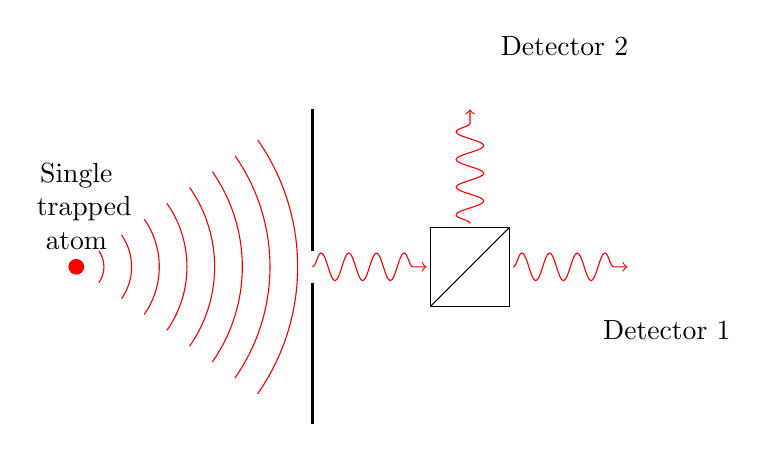
\begin{tikzpicture}
\draw (-0.5,-.5) rectangle +(1,1);
\draw (-.5,-.5) -- (.5,.5);
\draw[red,->,decorate, decoration={snake,amplitude=5,segment length=10, post length=.1cm}](-2,0)--(-.55,0) node[midway, above,shift=({0,.2cm})]{};
\draw[red,->,decorate, decoration={snake,amplitude=5,segment length=10, post length=.1cm}](.55,0)--(2,0);
\detector{1}{2.1}{0}{0}
\node at (2.5,-.8) {Detector 1};
\draw[red,->,decorate, decoration={snake,amplitude=5,segment length=10, post length=.1cm}](0,.55)--(0,2);
\detector{1}{0}{2.1}{90}
\node at (1.2,2.8) {Detector 2};
\fill[red] (-5,0) circle(0.1) node[above,black,text width=1cm,align=center,shift={(0,.1cm)}]{Single trapped atom};
\draw[red,decorate,decoration={expanding waves,angle=35}](-5,0) -- (-2,0);
\draw[thick] (-2,.2) -- (-2,2);
\draw[thick] (-2,-.2) -- (-2,-2);
\end{tikzpicture}
\end{figure}

What we measure is that we get an event on Detector 1 or Detector 2, but never on both of them at the same time. \marginnote{For experimental data on this, see, for example, PRL {\bf 39}, 691 (1977).} We measure the arrival of counts on the two detectors and count them up over a time interval. We find that each detector recorded about the same number of events and that the distribution between the two detectors is random.\marginnote{Why random? There could be ``hidden variables'' that we can't measure directly that tell which detector to record the event. There are experimental reasons that indicate that there aren't. Is the universe just weird? Are there many universes? We are going to take the ``shut up an calculate'' approach here and not worry about why questions.}

This situation calls for a new model. Nothing we've talked about prior to this point, from a classical perspective, tells us that we should expect the ElMaW to behave this way. Our classical model predicts that the wave will split at the beamsplitter and that half the intensity will go to Detector 1 and half to Detector 2.

There are lots of questions to ask: what happens to the ElMaW after the beamsplitter? Is the wave in both arms at the same time? If so, why do we not detect something at both detectors? If it is only in one arm, how do we know which? Why did it go one way and not the other? We obviously need more data.

\section{Polarizing Beamsplitter}
We use the polarization aspect of ElMaWs to say more about this new situation. We will put a polarizer between the atom and the beamsplitter so that only horizontally polarized waves pass through. Then we replace the beamsplitter with a {\em polarizing beamsplitter} (PBS). 
\begin{marginfigure}\centering
\begin{tikzpicture}[scale=1]
\draw[->,thick] (-.5,0,0) -- (4,0,0) node[right]{$x$};
\draw[->,thick] (0,0,0) -- (0,1.2,0) node[above]{$y$};
\draw[->,thick] (0,0,0) -- (0,0,1.2) node[left,below]{$z$};
\draw[color=blue,<->,thick](0,-.7,.6) -- (0,.6,-.7) node[above,black]{$\theta$};
\begin{scope}[canvas is zy plane at x=0]
\draw[dashed] (0,0,0) circle (.92);
\end{scope}
\draw[->,ultra thick](0,0,0) -- (1,0,0);
\begin{scope}[canvas is xz plane at y=.5,shift={(2,0,0)}]
\fill[black!40] (-.5,-.5) rectangle +(1,1);
\end{scope}
\begin{scope}[canvas is yz plane at x=2.5]
\fill[black!20] (-.5,-.5) rectangle +(1,1);
\end{scope}
\begin{scope}[canvas is xy plane at z=.5,shift={(2,0,0)}]
\fill[black!30] (-.5,-.5) rectangle +(1,1);
\end{scope}
\draw (1.5,.5,-.5) -- (2.5,.5,.5);
\draw (2,0,0.5) -- (2,0,2.5);
\draw[color=blue,<->,thick](3,-.5,0) -- (3,.5,0);
\draw[->,ultra thick] (2,0,.5) -- (2,0,2);
\draw[->,ultra thick] (2.5,0,0) -- (3.5,0,0);
\draw[color=blue,<->,thick](1.5,0,1.5) -- (2.5,0,1.5);
\node at (2,1.3,0) {PBS};
\end{tikzpicture}
\end{marginfigure}
This new tool reflects all of the incoming wave that has a horizontal polarization component and transmits the vertically polarized component. As with a polarizer, the transmitted electric field amplitude is $E_V = E_0 \cos\theta$ and the reflected field amplitude is $E_H = E_0 \sin\theta$. 

In terms of our setup, we arrange the PBS so that Detector 2 now gets all the horizontally polarized light and Detector 1 gets all the vertically polarized light. So, we send in horizontally polarized light and now we only measure events on Detector 2, never on Detector 1. If we rotate the initial polzarizer to be vertical, we only measure events on Detector 1, never on Detector 2. So far, so good. This is behaving like we expect for an ElMaW.

What happens down if we set the polarization angle to $\theta=\pm45^\circ$. We define these new directions as $D_R$ and $D_L$ for right- and left-diagonal.\begin{marginfigure}\centering
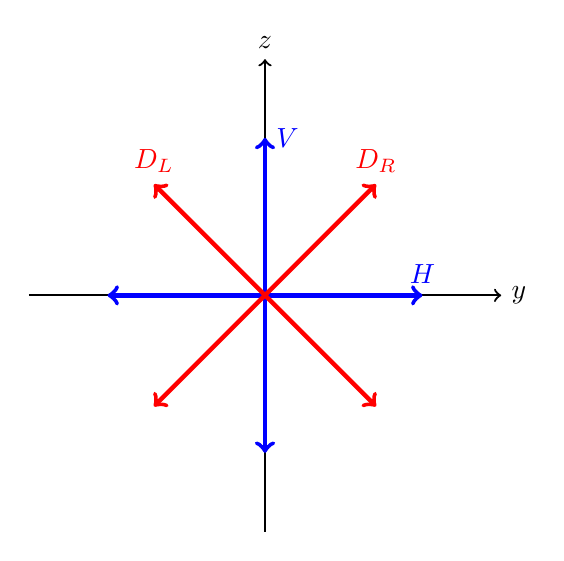
\begin{tikzpicture}[scale=1]
\draw[->,thick] (-3,0) -- (3,0) node[right]{$y$};
\draw[->,thick] (0,-3) -- (0,3) node[above]{$z$};
\draw[<->, blue,ultra thick] (-2,0) -- (2,0) node[above]{$H$};
\draw[<->, blue, ultra thick] (0,-2) -- (0,2) node[right]{$V$};
\draw[<->, red, ultra thick] (-1.41,-1.41) -- (1.41,1.41) node[above]{$D_R$};
\draw[<->, red, ultra thick] (1.41,-1.41)-- (-1.41,1.41) node[above]{$D_L$};
\end{tikzpicture}
\end{marginfigure}
With the incoming polarization set to either $D_L$ or $D_R$, we are back to measuring half of the events on Detector 1 and half on Detector 2 and never measuring an event at the same time.

\begin{exercise}
What is the second-order correlation for the following block of discrete bins measured at the output of the beamsplitter  where the intensity is measured in units of (distinct) electrons measured during the bin and where each bin is $100$~ns long?
\begin{table}
\centering
\begin{tabular}{|c||c|c|c|c|c|c|c|c|c|c|c|c|}
\hline
Detector 1 & 1 & 1 & 0 & 1 & 0 & 1 & 0 & 0 & 0 & 1 & 1 & 0 \\ 
\hline
Detector 2 & 0 & 0 & 1 & 0 & 1 & 0 & 1 & 1 & 1 & 0 & 0 & 1\\
\hline
\end{tabular}
\end{table}


\end{exercise}

\chapter{Rotated Measurements and Vector Spaces}
\section{Polarization Rotators}

We introduce a new tool here: a polarization rotator, also known as a half-wave (or $\lambda/2$) plate. What this tool does is rotate the polarization of the ElMaW without otherwise changing it. Unlike a polarizer, which blocks all the polarizations except one, a \hwp passes all polarizations, just rotating them by a specific angle $\phi$.
\begin{marginfigure}\centering
\begin{tikzpicture}[scale=1]
\draw[->,thick] (0,0,0) -- (3,0,0) node[right]{$x$};
\draw[->,thick] (0,0,0) -- (0,1,0) node[right]{$y$};
\draw[->,thick] (0,0,0) -- (0,0,1) node[right]{$z$};
\draw[color=blue,<->](.5,-.7,0) -- (.5,.7,0) node[above,black]{$\vec{E}$};
\begin{scope}[canvas is zy plane at x=1.3]
\fill[green, opacity=.2] (-1,-1) rectangle +(2,2);
\draw[dashed] (0,0) -- (0,1) node[above]{$\phi$};
\end{scope}
\draw[->,thick](1.3,0,0) node[below,text width=1cm,align=center]{\hwp}-- (1.3,.6,-.7) ;
\draw[color=blue,<->](2.3,-.45,.53) -- (2.3,.45,-.53) node[above,black]{$\vec{E}_\rmt{rotated}$};
\end{tikzpicture}
\end{marginfigure}

We take this new tool and place is before the PBS in our setup, which now looks like this:

\begin{figure}
\centering
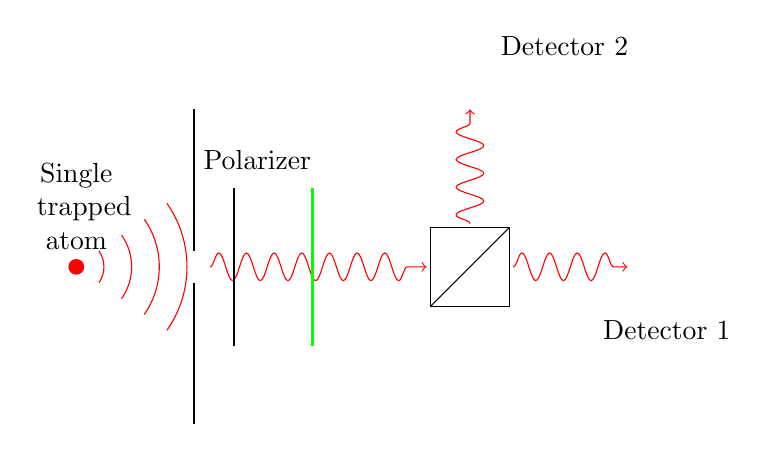
\begin{tikzpicture}
\draw (-0.5,-.5) rectangle +(1,1);
\draw (-.5,-.5) -- (.5,.5);
\draw[red,->,decorate, decoration={snake,amplitude=5,segment length=10, post length=.1cm}](-3.3,0)--(-.55,0) node[midway, above,shift=({0,.2cm})]{};
\draw[red,->,decorate, decoration={snake,amplitude=5,segment length=10, post length=.1cm}](.55,0)--(2,0);
\detector{1}{2.1}{0}{0}
\node at (2.5,-.8) {Detector 1};
\draw[red,->,decorate, decoration={snake,amplitude=5,segment length=10, post length=.1cm}](0,.55)--(0,2);
\detector{1}{0}{2.1}{90}
\node at (1.2,2.8) {Detector 2};
\fill[red] (-5,0) circle(0.1) node[above,black,text width=1cm,align=center,shift={(0,.1cm)}]{Single trapped atom};
\draw[red,decorate,decoration={expanding waves,angle=35}](-5,0) -- (-3.5,0);
\draw[thick] (-3.5,.2) -- (-3.5,2);
\draw[thick] (-3.5,-.2) -- (-3.5,-2);
\draw[thick] (-3,-1) -- (-3,1) node[above,shift={(.3,.1)}] {Polarizer};
\draw[thick,green] (-2,-1) node[below,black] {\hwp} -- (-2,1);
\end{tikzpicture}
\end{figure}

We are also going to assign a value to the measurements at each type of polarization. We will assign any measurement coming from Detector 1 as a $+1$ and any measurement from Detector 2 as a $-1$. We will use the following table to assign polarizations.
\begin{table}
\centering
\begin{tabular}{|c||c|c|}
\hline
\hwp angle & Detector 1 & Detector 2\\ 
\hline
$0^\circ$  & $V$ & $H$\\
\hline
$-45^\circ$  & $D_R$ & $D_L$\\
\hline
$90^\circ$  & $H$ & $V$\\
\hline
$45^\circ$  & $D_L$ & $D_R$\\
\hline
\end{tabular}
\end{table}

So we can now analyze the possible combinations between the polarizer angle $\theta = 0^\circ$ and the \hwp angle $\phi$ and what we get from the measurements.
\begin{itemize}
\item[\boldmath$\phi=0^\circ:$] We measure $+1$ on every measurement, 100\% of the time.
\item[\boldmath$\phi=90^\circ:$] We measure $-1$ on every measurement, 100\% of the time.
\item[\boldmath$\phi=45^\circ:$] We get a random result which is $+1$ about 50\% the time and $-1$ the other 50\%. 
\item[\boldmath$\phi=-45^\circ:$] We get a random result which is $+1$ about 50\% the time and $-1$ the other 50\%. 
\end{itemize}
We average all the measurements we get for a particular configuration. When we have probabilistic results the probability is calculated as the sum of the result value times the probability of measuring that value:

\bas
\rmt{Average Result} = & (\rmt{Result}_1)\times(\rmt{Probability of Result}_1) + \ldots \\
=& \sum_{n=1}^\rmt{All Results}(\rmt{Result}_n)(\rmt{Probability of Result}_n)
\eas

So for our $\phi=0^\circ$ case, the average is: $({+1})(1)=1$. For our $\phi=45^\circ$ case, the average is $({+1})(.5) + ({-1})(.5) = 0$. We keep adjusting the angles and find that the average results is $\cos(2\phi)$.

We interchange the detectors and find the same result. We move the detectors back and find the same result again. We obviously need a new model to describe what is going on after the the beamsplitter. We are going to call this new model a {\em Quantum State} model.\

\begin{exercise}
\label{exercise:rotatedhwp}
\begin{enumerate}
\item What are the polarizations that are measured by the  Detectors if we set the initial polarizer to $\theta=45^\circ$? Make a table like the one above for $\phi = 0^\circ, \pm 45^\circ$, and $90^\circ$. List what you expect to measure and with what probability.

\item Calculate the average results for all four $\phi$ angles from the previous part.
\end{enumerate}
\end{exercise}

\subsection{Propositions}
There is a handy piece of reasoning that we will make use of later that I want to introduce now. We start with something we can measure, like the outcome of tossing a six-sided die. This ideal die will roll $\{1,2,3,4,5,6\}$ with equal probability. We now ask questions called propositions:
\begin{itemize}
\item[Prop. A:] Is the result less than 3? It could be if it is $\{1,2\}$.
\item[Prop. B:] Is the result even? It could be if it is $\{2,4,6\}$.
\end{itemize}
We now ask {\em joint} propositions using the rules of logic.
\begin{itemize}
\item[Prop. A or B:] Is the result less than 3 {\bf or} even?  It could be if it is $\{1,2,4,6\}$.
\item[Prop. A and B:] Is the result less than 3 {\bf and} even? This is only possible if the result is $\{2\}$.
\end{itemize}

\begin{example}
Consider two propositions based on the roll of an 8-sided die:
\begin{itemize}
\item[Prop. A:] Is the result greater than 6?
\item[Prop. B:] Is the result divisible by 3?
\end{itemize}
For which measurement results will these propositions true? How about A and B as well as A or B?

\model We model the die as ideal - no result is weighted any more than any other.

\vis Not much to visualize for this problem.

\sol We have two possible results that satisfy Prop. A: ${7,8}$. There are two possible results that satisfy Prop. B: ${3,6}$. We therefore have the following joint proposition results: A {\em or} B: ${3,6,7,8}$. A {\em and} B: ${}$ - no result.

\assess The joint propositions are symmetric -- it does not matter which order we take first, A or B.

\end{example}

\section{Quantum Propositions}
\label{sec:quantprop}
We apply this same logic to the following two propositions about our measurement system where we've set the polarizer to $\theta = 0^\circ$:
\begin{itemize}
\item[Prop. A:] At $\phi=0^\circ$ do we measure ${+1}$ (or is the quantum state $V$)? Because we have the polarizer in place set to $V$ polarization, the answer to this question is that we always measure $+1$, 100\% of the time.
\item[Prop. B:] At $\phi=-45^\circ$ do we measure ${+1}$ (or is the quantum state $D_R$)? This is a little more challenging, because the answer is that sometimes we measure ${+1}$, but sometimes we measure ${-1}$, each with a 50\% probability. In any particular measurement, we might get ${+1}$, but there is no definite answer to this.
\end{itemize}
What about Prop. A or B? This is asking if the quantum state is $V$ or $D_R$. Since we will always measure a ${+1}$ for Prop. A, this joint proposition is always true. Now we try to measure Prop. A and B. We know that A is always true, since we've set the polarizer to $V$ ($\theta=0^\circ$). So we only need to adjust the \hwp to $-45^\circ$ and measure Prop. B. We find that this is ${+1}$ half the time and ${-1}$ the other half. So Prop. A and B is true 50\% of the time.

How about measuring Prop. B or A, where we reverse the order of measurement? To do this, we need to modify our  our experiment setup. Since Prop. B asks about a ${+1}$ measurement where $\phi_1=-45^\circ$, we'll leave Detector 1 where it is. In place of Detector 2, we'll add a second \hwp to rotate the polarization back to the original angle and a new set of detectors that behave just like our initial set. Detector 3 now corresponds to a ${+1}$ measurement and Detector 4 corresponds to a ${-1}$ measurement.

\begin{marginfigure}\centering
\centering
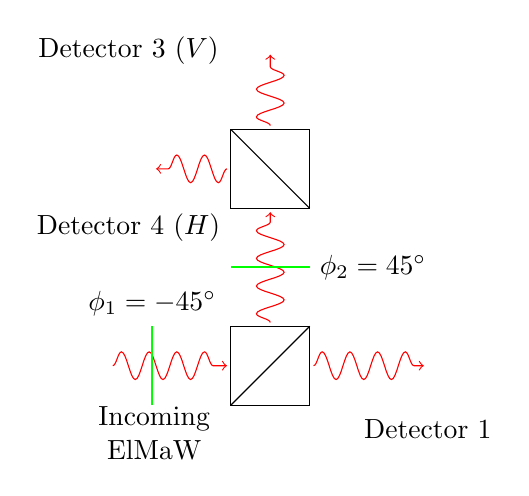
\begin{tikzpicture}
%PBS
\draw (-0.5,-.5) rectangle +(1,1);
\draw (-.5,-.5) -- (.5,.5);
%incoming beam
\draw[red,->,decorate, decoration={snake,amplitude=5,segment length=10, post length=.1cm}](-2,0)--(-.55,0) node[midway, below,shift=({-.2cm,-.4cm}),text width=2cm,black,align=center]{Incoming ElMaW};

\draw[thick,green] (-1.5,.5) node[above,black] {$\phi_1=-45^\circ$} -- (-1.5,-.5);

%outgoing beam to 1
\draw[red,->,decorate, decoration={snake,amplitude=5,segment length=10, post length=.1cm}](.55,0)--(1.95,0);
\detector{0.8}{2.1}{0}{0}
\node at (2,-.8) {Detector 1};
%beam to 2
\draw[red,->,decorate, decoration={snake,amplitude=5,segment length=10, post length=.1cm}](0,.55)--(0,1.95);

%PBS 2
\draw (-0.5,2) rectangle +(1,1);
\draw (-.5,3) -- (.5,2);

\draw[red,->,decorate, decoration={snake,amplitude=5,segment length=10, post length=.1cm}](0,3.05)--(0,3.95);

\detector{0.8}{0}{5.0}{90}
\node at (-1.8,4.0) {Detector 3 ($V$)};

\draw[red,->,decorate, decoration={snake,amplitude=5,segment length=10, post length=.1cm}](-.55,2.5)--(-1.45,2.5);
\detector{0.8}{-1.95}{3.2}{180}
\node at (-1.8,1.75) {Detector 4 ($H$)};

\draw[thick,green] (-.5,1.25) -- (.5,1.25)node[right,black] {$\phi_2=45^\circ$};

\end{tikzpicture}
\end{marginfigure}

So measuring Prop. B or A will give us ${+1}$ for B half of the time and then, since we've rotated back, will give us ${+1}$ on A half of the remaining times we measure. That means that Prop. B or A is true 75\% of the time. Compare this to the reverse which was true 100\% of the time. Clearly the ordering of our measurements matter. Our new quantum state model must take this into account and handle it. Finally, we ask about B and A. This is true 25\% of the time.\arnote{Work out this situation in your notes.}

\begin{exercise}
Consider two propositions where we have set the initial polarizer to $\theta=45^\circ$:
\begin{itemize}
\item[Prop. A:] At $\phi=0^\circ$ do we measure ${-1}$?
\item[Prop. B:] At $\phi=45^\circ$ do we measure ${+1}$?
\end{itemize}
For which measurement results will these propositions true? How about A and B as well as A or B? Finally, consider B and A as well as B or A.
\end{exercise}

\section{Linear Vector Spaces}
We are going to need a new set of mathematical tools to describe our quantum states. These are {\em vector spaces} which describe a set of relationships and interactions between the quantum states. \marginnote{A note about the word {\em vector}. We use vectors to describe position, momentum, forces, etc. in 3-space and 4-space. While that is one type of vector space, the tools we will be building here are much more general. Any time I want to refer to one of these types of vectors, I'll call it a 3-vector.} There are a number of different ways to represent a vector space in concrete form and we will make use of them as we go.

The quantum states are going to belong to a specific space of states called a {\em Hilbert Space}. We'll define this later, but it encompasses all of the possible quantum states of our system.

Our quantum vector space will be composed of elements, or states, called {\em ket-vectors} or just kets, written as $\ket{A}$. We will make use of complex numbers in this vector space and will represent them as $z$ and $w$.

In the quantum vector space, the following relationships hold between quantum states:\marginnote{We are following Susskind here.}
\begin{enumerate}
\item The sum of two kets is another ket:
\beq
\ket{A} + \ket{B} = \ket{C}
\eeq
\item Addition is commutative:
\beq
\ket{A} + \ket{B} = \ket{B} + \ket{A}
\eeq
\item Addition is associative:\marginnote{All of these relationships hold for 3-vectors, but where we only allow multiplication by real numbers.}
\beq
\left(\ket{A} + \ket{B}\right) +\ket{C} = \ket{A} + \left(\ket{B} + \ket{C}  \right)
\eeq
\item There exists a $0$ ket (usually written without the $\ket{\,}$) such that addition by it doesn't change a ket-vector:
\beq
\ket{A} + 0 = \ket{A}
\eeq
\item There exists a ``negative'' ket such that when you add to the positive ket, you get zero:
\beq
\ket{A} + \left({-\ket{A}} \right) = 0
\eeq
\item Multiplication by a complex number gives a new ket (note there are two equivalent ways of writing the multiplication):
\beq
z\ket{A} \equiv \ket{zA} = \ket{B}
\eeq
\item Multiplication by a complex number is distributive in a linear fashion:\marginnote{These last two constitute the conditions known as linearity.}
\beq
z\left(\ket{A} + \ket{B}  \right) = z\ket{A} + z\ket{B}
\eeq
\item and the same way here, too:
\beq
(z+ w)\ket{A} = z\ket{A} + w\ket{A}.
\eeq
\end{enumerate}

Wow, that was really abstract. There are a couple of ways we can make this more concrete. One way is to use complexe valued functions of some variable $x$. We'll explore these first:

\begin{example}
Show that $A(x) = 3+ \I x$ and $B(x) = 4 x - 6\I$ are both vector spaces.

\model We will model these two functions as complex functions of a real number $x$.

\vis Rats. It is hard to visualize things now. However, both of these functions are lines in the complex plane:
\begin{figure}
\centering
\begin{tikzpicture}[scale=0.3]
\draw[->,thick] (-10,0) -- (10,0) node[right]{Real};
\draw[->,thick] (0,-10) -- (0,10) node[above]{Imaginary};
\draw[color=blue,domain=-10:10] plot (3,\x);
\node[blue] at (5,1) {$A(x)$};
\draw[color=red,domain=-2.5:2.5] plot ({4*\x},-6);
\node[red] at (-6,-5) {$B(x)$};
\draw[color=green,domain=-2.5:2.5] plot ({3+4*\x},{\x-6});
\node[green] at (9,-3) {$(A+B)$};
\end{tikzpicture}
\end{figure}

\sol We just have to work through each of the pieces that make up a vector space and make sure that we end up with another complex-valued function. Here's the first two:
\begin{enumerate}
\item $\ket{A} + \ket{B} =  (3+ \I x) + (4 x - 6\I) = [3+4x + \I(x-6)]$ which is another complex-valued function (shown in green on the figure)
\item $\ket{B} + \ket{A} =   (4 x - 6\I) + (3+ \I x)  = [3+4x + \I(x-6)]$ which is the same thing we got before.\arnote{Your turn. Finish up the rest of these as practice.}
\end{enumerate}
\assess We stayed in the vector space for all the points which means that this type of linear, complex-valued function works as a concrete representation of a vector space.
\end{example}

\begin{exercise}
Show that a quadratic complex-valued function (you can invent your own as long as they have some kind of $x^2$ in them somewhere) also works to represent a vector space.
\end{exercise}

Another way we represent the vector space in a concrete form is to use matrices. We represent the ket as a column matrix. For simplicity we will make it a 1 by 2 matrix where each element $\alpha_k$ is a complex number.\marginnote{We will use the symbol $\Meq$ when we represent a vector with a matrix. It isn't really an equals because we are changing representations, but close.}
\beq
\ket{A}\Meq\vket{\alpha_1}{\alpha_2}
\eeq
This representation of a vector space also fulfills our requirements. For example:\arnote{Finish up showing that the matrix representation of the vector space also works for all the requirements.}
\beq
\ket{A} + \ket{B} \Meq \vket{\alpha_1}{\alpha_2} + \vket{\beta_1}{\beta_2} = \vket{\alpha_1 + \beta_1}{\alpha_2+\beta_2}
\eeq
and
\beq
z\ket{A}\Meq z\vket{\alpha_1}{\alpha_2} = \vket{z\alpha_1}{z\alpha_2}.
\eeq

\subsection{Bras and Kets}

We define a new vector space, related to the ket-vector called a {\em bra-vector} or a bra for short. These are writte as: $\bra{A}$ and follow all the same rules as the kets. The bra-vectors are related to the ket-vectors in the following way. In order to flip from a ket to a bra, we take the complex conjugate and we also reverse any ordering like this:
\beq
z\ket{A}\rightarrow \bra{A}z^*.
\eeq

In terms of our concrete matrix representation, we need to take the complex conjugate of all the elements {\em and} turn the column vector into a row vector.
\bas
\ket{A} \rightarrow & \bra{A} \\
\vket{\alpha_1}{\alpha_2} \rightarrow &  \vbra{\alpha_1^*}{\alpha_2^*}
\eas

\begin{exercise}
Show that the following two complex matrix vectors satisfy the requirements for our vector space:
\beq
\begin{pmatrix} 1+3\I \\ -4-\I \\ 7+6\I \end{pmatrix} \rmt{ and } 
\begin{pmatrix} 6 \\ 8+\I \\ -5\I \end{pmatrix}.
\eeq
\end{exercise}

\chapter{Quantum States and Vectors}

We continue developing the mechanics of working with vector spaces, then we will apply these to our quantum states.

\section{Inner Products}

We also define an inner product between a bra and a ket. This gives us a {\em bra-ket} or a bracket, which is where the names bra a ket come from. The inner product, or dot product, of two 3-vectors tells us how much one of the vectors lies along the direction of the other. The inner product takes two vectors as inputs and returns a complex number as the output.
\begin{marginfigure}\centering
\begin{tikzpicture}[scale=1]
\draw[->,red] (0,0) -- (3,1) node[right,black]{$\vec{V}_1$};
\draw[->,blue] (0,0) -- (1.8,2.8) node[above,black]{$\vec{V}_2$};

\draw [dashed] ($(0,0)!(1.8,2.8)!(3,1)$) coordinate(B) -- (1.8,2.8);

\draw[->,dashed,thick] (0,0)--(B);

\end{tikzpicture}
\end{marginfigure}
We note the inner product between a bra and a ket as
\bas
\bra{A}\ket{B}\equiv \avg{A|B}.
\eas
If we reverse the order of the inner product, we have to take the complex conjugate of the output in order to follow our bra-to-ket rule above: $\avg{A|B} = \avg{B|A}^*$.

The representation of the inner product in terms of matrices is the product of a row matrix (the bra) and a column matrix (the ket):
\beq
\avg{A|B}\Meq\vbra{\alpha_1^*}{\alpha_2^*}\vket{\beta_1}{\beta_2} = \alpha_1^*\beta_1 + \alpha_2^*\beta_2
\eeq\marginnote[-1cm]{In terms of 3-vectors, the dot product of two vectors in terms of their components is $\vec{a}\cdot\vec{b}=a_x b_x + a_yb_y + a_zb_z$.}

\subsection{Normalization}
Following a couple of other definitions from 3-vectors, we can talk about the ``magnitude'' of a state vector in our quantum state space by taking the inner product of a state vector with itself: $\avg{A|A}$. We are mostly going to be working with state vectors that are {\em normalized}, where their magnitude is $1$:
\beq
\avg{A|A} = 1.
\eeq

\subsection{Orthogonality}
We also borrow the idea of two state vectors being {\em orthogonal} from our 3-vector concepts. Two 3-vectors are orthogonal if their dot product is zero. We define a similar concept for our state vectors. $\ket{A}$ and $\ket{B}$ are orthogonal if
\beq
\avg{A|B} = 0.
\eeq

\begin{exercise}
\label{ex:statevector}
You are given the quantum state 
\beq
\ket{A} \Meq \vket{2+3\I}{-4}.
\eeq
\begin{enumerate}
\item Normalize the state vector.
\item Find another normalized state vector that is orthogonal to $\ket{A}$
\end{enumerate}
\end{exercise}

\section{Orthonormal Basis Vectors}

It is really handy when we work with 3-vectors to break a vector up in terms of its components in some orthogonal basis of unit vectors. For example, we can write the vector $\vec{V}$ as $\vec{V} = V_x\hat{x} + V_y\hat{y} + V_z\hat{z}$. \marginnote{We could have picked a different basis, for example, polar basis 3-vectors: $\vec{V}=V_r\hat{r}+V_\theta\hat{\theta}+V_\phi\hat{\phi}$. The same thing applies to this set of orthonormal basis 3-vectors.} The unit vectors all have the properties where they are normalized: $\hat{x}\cdot\hat{x}=1$ and they are orthogonal: $\hat{x}\cdot\hat{y}=0$. We put both of these together and call the set of basis 3-vectors {\em orthonormal}.
We write our 3-vector in terms of these basis 3-vectors by finding the piece of the 3-vector that lies along the basis vector ($V_x = \vec{V}\cdot\hat{x}$), repeating the same thing for the other basis 3-vectors, then adding them together.

We now do the same thing for our quantum state vectors. We want to work in general, so we won't be specific yet about the representation of our basis vectors, but we'll be able to specify them later. For now, we will say we have a set of basis vectors $\ket{j}$.\marginnote[-1cm]{We can do this with 3-vectors by defining $\hat{x}_j$ where $j=1,2,3$ and $\hat{x}_1 \equiv \hat{x}$, $\hat{x}_2\equiv\hat{y}$, etc.} We decompose any quantum state vector in terms of the basis vectors in the same way as with 3-vectors:
\toolnote{\toollabel{tool:decom}{\includegraphics{tool1.tikz} {\bf Orthonormal Basis Decomposer}}  This tool is used to write a state vector in terms of a set of orthonormal basis vectors.} 
\beq
\ket{A} = \sum_j \alpha_j \ket{j},
\label{eq:decom}
\eeq
where $\alpha_j$ are complex numbers replacing the $V_x$, $V_y$, etc. from the 3-vector example.

We follow our pattern from 3-vectors to figure out what the $\alpha_j$ complex numbers should be in our $\ket{j}$ basis. We first need to do two things: 1) define the bra version of the basis which we will call $\bra{k}$. \marginnote{Note that $\bra{j}$ and $\bra{k}$ are both in the same set of possible basis states.} We now take the inner product of this basis bra-vector with our state vector:
\beq
\avg{k|A}=\sum_j\bra{k}\alpha_j \ket{j}.
\eeq
Now we can use the fact that our basis vectors are orthogonal so that if $k=j$ then $\avg{j|j}=1$. Otherwise, $\avg{k|j}=0$. We can write this in terms of the Kronecker delta:
\beq
\delta_{kj} = \begin{cases}1 &\rmt{ if } j=k, \\ 0 &\rmt{ if }j\neq k.\end{cases}
\label{eq:kronecker_eqn}
\eeq
So we now have $\avg{k|j}=\delta_{kj}$. This is a very useful tool since now the sum over $j$ simplifies. The only term that isn't zero is the one where $k=j$, and that one is just $\alpha_{k}$. This is a new tool, written in general gives us
\toolnote{\toollabel{tool:orthog}{\includegraphics{tool2.tikz} {\bf Orthonormal Collapser}}  This tool is used to collapse a sum using the inner product of two orthonormal state vectors.} 
\beq
\avg{k|A} = \bra{k} \left( \sum_j \alpha_j \ket{j} \right)= \alpha_k.
\label{eq:orthog}
\eeq
So we have (replacing $k$ with $j$ to emphasise that it doesn't matter what symbol we use to describe our basis states)
\beq
\avg{j|A} = \alpha_j.
\eeq

There is one more trick we can use here. We insert this back into our decomposition of $\ket{A}$ in terms of its basis vectors, Eq.~(\ref{eq:decom})
\beq
\ket{A} = \sum_j\avg{j|A}\ket{j}.
\eeq
Since $\avg{j|A}$ is just a complex number, we can write it before or after the vector. So we write it after and get
\beq
\ket{A} = \sum_j \ket{j}\bra{j} \ket{A}.
\eeq
This implies that the combination of the sum and the ket-bra vectors must be $1$. This is a really useful tool that we will come back to again and again.
\toolnote{\toollabel{tool:span}{\includegraphics{tool3.tikz} {\bf Completeness Spanner}}  This tool is used to insert a complete set of basis vectors and project a state vector onto that basis.} 
\beq
\sum_j \ket{j}\bra{j} = 1
\label{eq:span}
\eeq
This is also known as the completeness relationship because it works since the basis vectors $\ket{j}$ form a complete basis.

Now that we have this handful of tools, we are ready to go back to our quantum ElMaW system and use these tools to model that system.

\begin{example}
I give you a complete set of orthonormal basis vectors: $\{\ket{0},\ket{1},\ket{2},\ket{3},\ket{4} \}$ and a vector $\ket{A} = 3\ket{0} + 2\I \ket{1} + (-3+4\I)\ket{3} - 6\ket{4} $ decomposed in this basis.
\begin{enumerate}
\item Show that the orthogonality collapser, Eq.~(\ref{eq:orthog}), gives the components of the vector $\ket{A}$.
\item Show that the completeness spanner, Eq.~(\ref{eq:span}), equal $1$.
\end{enumerate}

\model We are modeling the given set of basis vectors as being complete- they cover all possibilities in our Hilbert space.

\vis It is hard to visualize a 5-dimensional vector space, though it is just a vector pointing is some direction.

\sol We first want to use the \ref{tool:orthog} tool to decompose the vector into its basis states. We begin by projecting each one of the basis vectors onto our given vector $\ket{A}$. We start with the $\bra{0}$ basis vector:
\beq
\avg{0|A} =  3\avg{0|0} + 2\I \avg{0|1} + 0 \avg{0|2} + (-3+4\I)\avg{0|3} - 6\avg{0|4} = 3, 
\eeq
because of the nature of the orthogonal basis vectors (Eq.~(\ref{eq:kronecker_eqn}). We continue with the other basis vectors to get
\bas
\avg{1|A} =& 2\I & \avg{2|A} =& 0 \\
\avg{3|A} = & (-3+4\I) & \avg{4|A} = & -6
\eas

We now try out the \ref{tool:span} tool. This means we multiply out
\beq
\left(\sum_j \ket{j}\bra{j}\right)\ket{A} = \left( \ket{0}\bra{0} +\ket{1}\bra{1} +\ket{2}\bra{2} +\ket{3}\bra{3} +\ket{4}\bra{4}   \right) \ket{A}.
\eeq
We simplify our calculations noting that the only terms that will be non-zero are the terms like $\ket{0}\bra{0}\ket{0}$ since the other terms like $\ket{3}\bra{3}\ket{1}$ are zero due to the orthogonality condition of the basis vectors. After we expand out the product and simplify we are left with\arnote{Write out this product in your notes and make sure you get this result.}
\beq
\left(\sum_j \ket{j}\bra{j}\right) \ket{A} = 3\ket{0} + 2\I \ket{1} + (-3+4\I)\ket{3} - 6\ket{4} 
\eeq

\assess This gives us $\ket{A}$, so we find that the\ref{tool:span} must be 1, as expected.

\end{example}

\section{Modeling Quantum States}

We go back to our ElMaW model where we look at the emission of an electromagnetic wave from a single atom. The wave passes through a polarizer (angle $\theta$), then a \hwp (angle $\phi$), then to our PBS and our detectors.
\begin{marginfigure}\centering
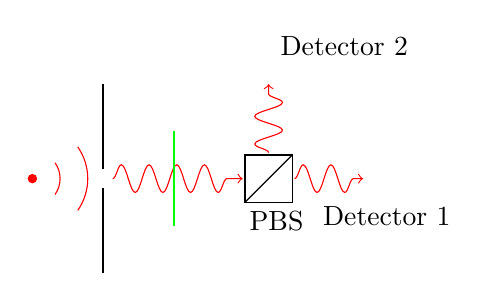
\begin{tikzpicture}[scale=0.6]
\draw (-0.5,-.5) rectangle +(1,1) node[below,shift={(-.2,-.6)}]{PBS};
\draw (-.5,-.5) -- (.5,.5);
\draw[red,->,decorate, decoration={snake,amplitude=5,segment length=10, post length=.1cm}](-3.3,0)--(-.55,0) node[midway, above,shift=({0,.2cm})]{};
\draw[red,->,decorate, decoration={snake,amplitude=5,segment length=10, post length=.1cm}](.55,0)--(2,0);
\detector{1}{2.1}{0}{0}
\node at (2.5,-.8) {Detector 1};
\draw[red,->,decorate, decoration={snake,amplitude=5,segment length=10, post length=.1cm}](0,.55)--(0,2);
\detector{1}{0}{2.1}{90}
\node at (1.6,2.8) {Detector 2};
\fill[red] (-5,0) circle(0.1);
\draw[red,decorate,decoration={expanding waves,angle=35}](-5,0) -- (-3.5,0);
\draw[thick] (-3.5,.2) -- (-3.5,2);
\draw[thick] (-3.5,-.2) -- (-3.5,-2);
%\draw[thick] (-3,-1) -- (-3,1) node[above,shift={(.5,.1)}] {Polarizer};
\draw[thick,green] (-2,-1) node[below,black] {\hwp} -- (-2,1);
\end{tikzpicture}
\end{marginfigure}
Now we remove the polarizer and set \hwp to $0^\circ$. We get results ${\pm 1}$ on the two detectors. We now define the states where we measure ${+1}$ as the state vector $\ket{V}$ and the states where we measure ${-1}$ as $\ket{H}$.

\subsection{Paramatrization}

Are $\ket{V}$ and $\ket{H}$ a complete set of basis vectors? How many basis vectors do we need to describe the direction of the polarization? For a free propagating ElMaW, there are two degrees of freedom. For a general 3-vector, there are also two degrees of freedom (the polar angles $\theta$ and $\phi$). So we need two parameters to specify an arbitrary quantum state. We will write the state as
\beq
\ket{A} = \alpha_V\ket{V} + \alpha_H\ket{H}
\label{eq:adecomp}
\eeq\marginnote[-1cm]{Using \ref{tool:decom}}%
where $\alpha_H$ and $\alpha_V$ are complex numbers. \marginnote[1cm]{This may look like 4 parameters (two complex numbers), but it is only 2 since we will need to normalize $\ket{A}$ and since there is an overall arbitrary complex phase factor since $\E{\I\beta}\E{-\I\beta}=1$.} So, $\ket{V}$ and $\ket{H}$ look like they might work for basis vectors. Are they normalized? What is $\avg{V|V}$? We know that if we start with a $V$-polarized wave and send it through a $V$ polarizer, it doesn't change the polarization. That is good evidence that $\avg{V|V}=1$. 

Are $\ket{V}$ and $\ket{H}$ orthogonal? If we send a $V$-polarized wave through a $H$ polarizer, none of the wave passes. That looks like evidence that $\avg{V|H}=0$.

\section{Probabilities}

Going back to our arbitrary state vector $\ket{A} = \alpha_H\ket{H}+\alpha_V\ket{V} $, we use the Orthogonality Collapser to see what happens when we send the $\ket{A}$ through a $V$-oriented polarizer:
\beq
\begin{split}
\avg{V|A} &= \alpha_V \rmt{ and likewise}\\
\avg{H|A} &= \alpha_H
\end{split}
\label{eq:vandhcomponents}
\eeq\marginnote[-1.5cm]{Using \ref{tool:orthog}}%
This seems to indicate that $\alpha_V$ and $\alpha_H$ are related to what we measure on our detectors. But they are complex numbers, which isn't good for a probability --- we can't measure complex probabilities. We will, instead, define the probability $P$ of measuring 
\beq
P(\rmt{measuring }{+1} \rmt{ \ie } \ket{V}) = \alpha_V^*\alpha_V.
\label{eq:ampprob}
\eeq
We use a bit of complex notation shorthand ($\alpha_V^*\alpha_V = \abs{\alpha_V}^2$) and Eq.~(\ref{eq:vandhcomponents}) to write $\alpha_V=\avg{V|A}$ which gives us a new tool for predicting the probability of measuring a particular outcome:
\toolnote{\toollabel{tool:prob}{\includegraphics{tool4.tikz} {\bf Probability Predictor}}  This tool is used to calculate the probability of measuring a particular outcome of a quantum state.}%
\beq
P(\rmt{measuring } \ket{V}) = \abs{\avg{V|A}}^2.
\label{eq:prob}
\eeq%
It is important to note that we've set the \hwp to $0^\circ$. That means we are measuring in the $V-H$ basis and it makes sense to use $\ket{H}$ and $\ket{V}$ as our orthonormal basis states.

Ok, what do we get now if we check the normalization of $\ket{A}$?\arnote[.5cm]{Expand the parenthesis and then use the orthonormal nature of $\ket{V}$ and $\ket{H}$ to simplify.}
\bas
\avg{A|A} = &\left(\bra{H}\alpha_H^* +\bra{V}\alpha_V^*\right)\left(\alpha_H\ket{H}+\alpha_V\ket{V}\right)\\ =& \alpha_H^*\alpha_H + \alpha_V^*\alpha_V 
\eas
But we make sure that all of our quantum state vectors are all normalized so that $\avg{A|A}=1$. Combining this with Eq~(\ref{eq:ampprob}) gives us
\beq
P(\rmt{measuring } \ket{V}) + P(\rmt{measuring } \ket{H}) =1.
\eeq
This is good. It means that we have a 100\% chance of measuring something.

\begin{exercise}
Starting with the quantum state 
\beq\ket{A} = \frac{1+\I}{\sqrt{3}} \ket{V} + \frac{\I}{\sqrt{3}}\ket{H},
\eeq

\begin{enumerate}
\item Check that $\ket{A}$ is normalized.
\item What is the probability of measuring $\ket{V}$?
\item What is the probability of measuring $\ket{H}$?
\item Is the total probability equal to $1$?
\end{enumerate}

\end{exercise}

\section{A Second Orthonormal Basis}
\begin{marginfigure}[2cm]
\centering
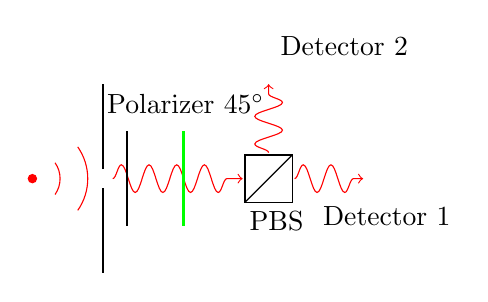
\begin{tikzpicture}[scale=0.6]
\draw (-0.5,-.5) rectangle +(1,1) node[below,shift={(-.2,-.6)}]{PBS};
\draw (-.5,-.5) -- (.5,.5);
\draw[red,->,decorate, decoration={snake,amplitude=5,segment length=10, post length=.1cm}](-3.3,0)--(-.55,0) node[midway, above,shift=({0,.2cm})]{};
\draw[red,->,decorate, decoration={snake,amplitude=5,segment length=10, post length=.1cm}](.55,0)--(2,0);
\detector{1}{2.1}{0}{0}
\node at (2.5,-.8) {Detector 1};
\draw[red,->,decorate, decoration={snake,amplitude=5,segment length=10, post length=.1cm}](0,.55)--(0,2);
\detector{1}{0}{2.1}{90}
\node at (1.6,2.8) {Detector 2};
\fill[red] (-5,0) circle(0.1);
\draw[red,decorate,decoration={expanding waves,angle=35}](-5,0) -- (-3.5,0);
\draw[thick] (-3.5,.2) -- (-3.5,2);
\draw[thick] (-3.5,-.2) -- (-3.5,-2);
\draw[thick] (-3,-1) -- (-3,1) node[above,shift={(.75,.1)},text width=2cm, align=left] {Polarizer $45^\circ$};
\draw[thick,green] (-1.8,-1) node[below,black] {\hwp} -- (-1.8,1);
\end{tikzpicture}
\end{marginfigure} We return back to our setup and this time we add the polarizer back in and turn it to $45^\circ$.\marginnote{We saw in Exercise \ref{exercise:rotatedhwp} that we needed to put the \hwp at ${-45}^\circ$ in order to measure in this basis.} This means we are preparing a new, specific state with polarization $D_R$. We know from our previous experiments that we should expect to measure ${+1}$ half of the time and to measure ${-1}$ the other half, with random results on each measurement. Using our probability model, we expect that the quantum state after the polarizer to be something like
\beq
\ket{D_R} = \frac{1}{\sqrt{2}}\ket{V} + \frac{1}{\sqrt{2}}\ket{H}.
\label{eq:drcomp}
\eeq
That state has everything we need in it - the probabilities all work out and the measurements we get from it agree with our experiment results and it is normalized. Is there another normalized basis vector $\ket{D_L}$ that is orthogonal to $\ket{D_R}$? We write $\ket{D_L}$ as an arbitrary vector $\ket{D_L} = \alpha_H\ket{H} + \alpha_V\ket{V}$ and then take the inner product with $\ket{D_R}$ and set that to zero. Doing this we find that \arnote{Do this on your own and check your work!}
\beq
\ket{D_L}  = \frac{1}{\sqrt{2}}\ket{V} - \frac{1}{\sqrt{2}}\ket{H}.
\label{eq:dlcomp}
\eeq

We are doing all of these measurements in the $V-H$ basis with the \hwp at $0^\circ$. We could, however, rotate the \hwp to $-45^\circ$ and measure in the $D_R-D_L$ basis. We can invert these two equations to see what $\ket{H}$ and $\ket{V}$ would be in this basis. We get\arnote{You need to work this one, too!}
\bas
\ket{V} =&\frac{1}{\stwo}\ket{D_R} + \frac{1}{\stwo}\ket{D_L}\\
\ket{H} =& \frac{1}{\stwo}\ket{D_R} - \frac{1}{\stwo}\ket{D_L}.
\eas
%
\begin{example} 
What is the arbitrary vector $\ket{A} = \frac{4}{5}\ket{V} + \frac{3\I}{5} \ket{H}$ in the $D_R-D_L$ basis?

\model We are given a state prepared in the $V-H$ basis, so we model this with the polarizer at some angle $\theta$ that gives us this state. We set the \hwp at ${-45}^\circ$ to measure in the $D_R-D_L$ basis.

\vis Our picture is the same as we've used before, shown in Figure \ref{fig:polexamplefig}.
\begin{figure}
\centering
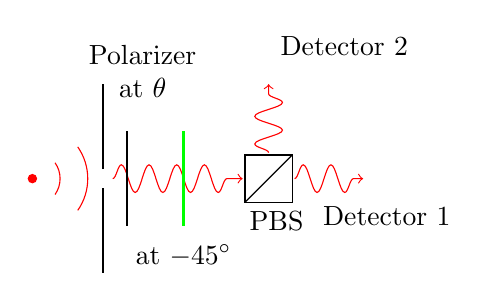
\begin{tikzpicture}[scale=0.6]
\draw (-0.5,-.5) rectangle +(1,1) node[below,shift={(-.2,-.6)}]{PBS};
\draw (-.5,-.5) -- (.5,.5);
\draw[red,->,decorate, decoration={snake,amplitude=5,segment length=10, post length=.1cm}](-3.3,0)--(-.55,0) node[midway, above,shift=({0,.2cm})]{};
\draw[red,->,decorate, decoration={snake,amplitude=5,segment length=10, post length=.1cm}](.55,0)--(2,0);
\detector{1}{2.1}{0}{0}
\node at (2.5,-.8) {Detector 1};
\draw[red,->,decorate, decoration={snake,amplitude=5,segment length=10, post length=.1cm}](0,.55)--(0,2);
\detector{1}{0}{2.1}{90}
\node at (1.6,2.8) {Detector 2};
\fill[red] (-5,0) circle(0.1);
\draw[red,decorate,decoration={expanding waves,angle=35}](-5,0) -- (-3.5,0);
\draw[thick] (-3.5,.2) -- (-3.5,2);
\draw[thick] (-3.5,-.2) -- (-3.5,-2);
\draw[thick] (-3,-1) -- (-3,1) node[above,shift={(.2,.3)},text width=2cm, align=center] {Polarizer at $\theta$};
\draw[thick,green] (-1.8,-1) node[below,black,text width=2.5cm, align=center,shift={(0,-.1)}] {\hwp at ${-45}^\circ$} -- (-1.8,1);
\end{tikzpicture}
\caption[][2cm]{ }
\label{fig:polexamplefig}
\end{figure}

\sol We use the relationships between the two basis sets to plug in for $\ket{V}$ and $\ket{H}$. Simplifying, we get \arnote{More things for you to work out! Both the substitution and the normalization.}
\beq
\ket{A} = \frac{4+3\I}{5\sqrt{2}} \ket{D_R} + \frac{4-3\I}{5\sqrt{2}} \ket{D_L}. 
\eeq

\assess We better check the normalization of our state:
\bas
\avg{A|A} =& \left(\frac{4-3\I}{5\sqrt{2}} \bra{D_R} + \frac{4+3\I}{5\sqrt{2}} \bra{D_L}\right) \left(\frac{4+3\I}{5\sqrt{2}} \ket{D_R} + \frac{4-3\I}{5\sqrt{2}} \ket{D_L}\right)\\
=& 1.
\eas
Our normalization works. Good.

\end{example}
%

%
\begin{exercise}
What are the probabilities of measuring ${+1}$ and ${-1}$ if we send the following state: 
$\ket{A} = \frac{\I}{2}\ket{V} + \frac{\sqrt{3}}{2}\ket{H}$ into our measurement system with the \hwp at ${-45}^\circ$?

\end{exercise}


\section{One more Basis}
\label{sec:ybasis}
We now have two different sets of basis vectors. But, in principle, the polarization of the ElMaW could point in one more direction! This is known as {\em circular} polarization and it corresponds to a phase shift between the $x$ and $y$ components of the electric field vector. This is written (using the CEWAM) as either {\em right-handed}
\begin{marginfigure}\centering
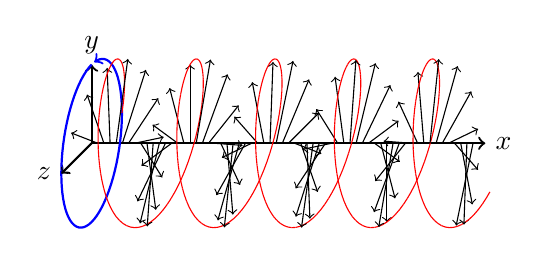
\begin{tikzpicture}[scale=1]
\draw[->,thick] (0,0,0) -- (5,0,0) node[right]{$x$};
\draw[->,thick] (0,0,0) -- (0,1,0) node[above]{$y$};
\draw[->,thick] (0,0,0) -- (0,0,1) node[left]{$z$};

\draw [->,thick,blue] (0,1,0) \foreach \t in {0,5,...,355}{
        -- (0,cos \t, sin \t) } ;

\foreach \k [evaluate={%
    \i=\k*5.625; 
    \j=\i>0 ? \i-5.625 : 0; 
    \a=90-\i; 
    \b=90-\j; 
    \c=int(mod(\k,5));}] 
    in {0,...,310}{
        \ifnum\c=0
            \draw [->] (\i/360,0,0) -- ++(0,cos \a, sin \a);
        \fi
        \draw [red] (\i/360,cos \a, -sin \a) -- (\j/360,cos \b, -sin \b);
    }
\end{tikzpicture}
\end{marginfigure}

\beq
\vec{E}_{C_R} = \frac{1}{\stwo}E_0\E{\I(kx-\omega t)}(\hat{y} + \I \hat{z})
\eeq
or as {\em left-handed} circular polarization:
\begin{marginfigure}\centering
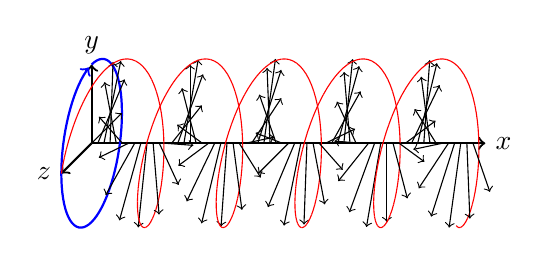
\begin{tikzpicture}[scale=1]
\draw[->,thick] (0,0,0) -- (5,0,0) node[right]{$x$};
\draw[->,thick] (0,0,0) -- (0,1,0) node[above]{$y$};
\draw[->,thick] (0,0,0) -- (0,0,1) node[left]{$z$};

\draw [->,thick,blue] (0,1,0) \foreach \t in {0,5,...,355}{
        -- (0,cos \t, -sin \t) } ;

\foreach \k [evaluate={%
    \i=\k*5.625; 
    \j=\i>0 ? \i-5.625 : 0; 
    \a=90-\i; 
    \b=90-\j; 
    \c=int(mod(\k,5));}] 
    in {0,...,310}{
        \ifnum\c=0
            \draw [->] (\i/360,0,0) -- ++(0,cos \a, -sin \a);
        \fi
        \draw [red] (\i/360,cos \a, sin \a) -- (\j/360,cos \b, sin \b);
    }
\end{tikzpicture}
\end{marginfigure}
\beq
\vec{E}_{C_L} = \frac{1}{\stwo}E_0\E{\I(kx-\omega t)}(\hat{y} - \I \hat{z})
\eeq

Experimentally, we can turn linear polarization into circular polarization using a {\em quarter wave-plate} also written as a \qwp. We place the \qwp  between the polarizer and the \hwp. If we set the \qwp to $C_R$ or $C_L$ polarization, then it doesn't matter whether we measure in the $V-H$ or the $D_R-D_L$ basis, we measure half of the events at Detector 1 and half at Detector 2. This is evidence that the $C_R-C_L$ basis is orthogonal to both of the other bases. Because the ElMaW can point in any direction in 3-vector space, we need one more orthonormal set of basis vectors to cover all the possibilities. One set that works is:
\bas
\ket{C_R} = & \frac{1}{\stwo}\ket{V} + \frac{\I}{\stwo}\ket{H} \\
\ket{C_L} = & \frac{1}{\stwo}\ket{V} - \frac{\I}{\stwo}\ket{H}.
\label{eqn:circular_pol_basis}
\eas
%
\begin{example}
Does the model for circularly polarized quantum states work? 
\begin{enumerate}
\item Is it orthonormal?
\item Is it orthogonal to the other bases?
\item Does it make the expected prediction for measurement results?
\end{enumerate}

\model We will use the basis decomposition given in Eq.~(\ref{eqn:circular_pol_basis}) and work this out using the $\ket{V}$ and $\ket{H}$ basis, which we know is orthonormal.
\begin{marginfigure}
\centering
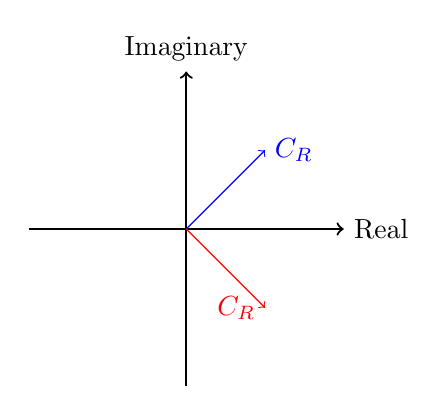
\begin{tikzpicture}[scale=0.2]
\draw[->,thick] (-10,0) -- (10,0) node[right]{Real};
\draw[->,thick] (0,-10) -- (0,10) node[above]{Imaginary};
\draw[->,blue] (0,0) -- (5,5)node[right] {$\ket{C_R}$};
\draw[->,red] (0,0) -- (5,-5) node[left]{$\ket{C_R}$};
\end{tikzpicture}
\caption{ }
\label{fig:circularpol_vectors}
\end{marginfigure}

\vis Again it is hard to visualize these vectors since they exist in the imaginary plane. But in that plane they look to be orthogonal as shown in figure~\ref{fig:circularpol_vectors}.

\sol We first check that the vectors are normalized:\arnote{Expand out the products to check that they work.}
\bas
\avg{C_R|C_R} = & \left(\frac{1}{\stwo}\bra{V} + \frac{-\I}{\stwo}\bra{H} \right) \left(\frac{1}{\stwo}\ket{V} + \frac{\I}{\stwo}\ket{H} \right)\\
= & \frac{1}{2} + \frac{1}{2} = 1\\
\avg{C_L|C_L} = & \left(\frac{1}{\stwo}\bra{V} + \frac{\I}{\stwo}\bra{H} \right) \left(\frac{1}{\stwo}\ket{V} + \frac{-\I}{\stwo}\ket{H} \right)\\
= & 1
\eas
Similarly, we check for orthogonality:
\bas
\avg{C_R|C_L} = & \left(\frac{1}{\stwo}\bra{V} + \frac{-\I}{\stwo}\bra{H} \right) \left(\frac{1}{\stwo}\ket{V} + \frac{-\I}{\stwo}\ket{H} \right)\\
= & \frac{1}{2} - \frac{1}{2} = 0.
\eas
The next thing we want to know is if this basis is orthogonal to the other bases:
\bas
\avg{V|C_R} = & \frac{1}{\stwo} \\
\avg{D_R|C_R} = & \frac{1}{2} + \frac{\I}{\stwo},
\eas
so we see it is not orthogonal to either of the other bases. Finally, we look at the probability of measuring $\ket{V}$ and $\ket{H}$ using the \ref{tool:prob}:
\bas
P(\ket{V}) = & \abs{\avg{V|C_R} }^2= \frac{1}{2}\\
P(\ket{H}) = & \abs{\avg{H|C_R} }^2= \frac{1}{2}.
\eas

\assess The probabilities add up to 1, so we have maintained the normalization condition.


\end{example}

\section{Matrix Representation}

It is sometimes useful to use the matrix representation when working with quantum states. Therefore, we want to represent $\ket{V}$ and $\ket{H}$ in terms of matrices. How big are the matrices? Well, we saw previously that we need two free parameters to describe a state. So our matrices better have two complex numbers. The following matrices work:
\bas
\ket{V}&\Meq\vket{1}{0}\\
\ket{H}&\Meq\vket{0}{1}
\eas
We then write any arbitrary state vector in terms of these basis matrices (Eq.~(\ref{eq:adecomp}))\marginnote{Using \ref{tool:decom}}
\beq
\ket{A} \Meq \alpha_V\vket{1}{0} + \alpha_H\vket{0}{1} = \vket{\alpha_V}{\alpha_H}.
\eeq

\begin{exercise}
In Exercise \ref{ex:statevector}, you started with the quantum state vector
\beq
\ket{A}\Meq \vket{2+3\I}{-4}
\eeq
and normalized it. Assuming that the state vector is written in the $V-H$ basis and measured in that same basis, what is the probability you will measure an outcome of $+1$? $-1$? What is the expected average of many measurements?

\end{exercise}

\chapter{A New Quantum System}
Now that we have a model for describing a quantum system (our ElMaW from a single atom), let's use this model to describe another quantum system: spin.

\section{Atomic Magnetic Dipole Moment}

We are interested in measuring the intrinsic magnetic dipole moment of atoms. Why? Because this will turn out to be a quantum system very similar to our ElMaW system. How do we go about doing this? Well, there is an interaction between the magnetic dipole moment and an external magnetic field. The potential energy is $V={-\vec{\mu}\cdot\vec{B}}$.
\begin{marginfigure}\centering
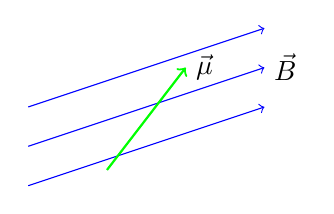
\begin{tikzpicture}[scale=1]
\draw[->,blue] (0,0) -- (3,1);
\draw[->,blue] (0,0.5) -- (3,1.5) node[right,black]{$\vec{B}$};
\draw[->,blue] (0,1) -- (3,2);
\draw[->,green,thick] (1,0.2) -- (2,1.5) node[right,black]{$\vec{\mu}$};

\end{tikzpicture}
\end{marginfigure}
But this interaction just turns the dipole so that it aligns with the magnetic field. Measuring the turning of a single atom is hard. It would be better if we could make this into a force. Then we could apply the force over some distance and measure the displacement or the change in kinetic energy. From classical physics, we know that $\vec{F}=-\vec{\nabla} V = \vec{\mu}\cdot(\vec{\nabla}\cdot\vec{B})$, so if we could make a magnetic field gradient, then the dipole would feel a force and we could measure this. We will model the magnetic field gradient as being only in a single direction (the $z$ direction). That means the force we are looking for is
\beq
\vec{F} = \mu_z \frac{\partial B_z}{\partial z}\hat{z}.
\eeq
\begin{marginfigure}\centering
\begin{tikzpicture}[scale=1]
\draw[->] (0,1,0) -- (.5,1,0) node[right]{$y$};
\draw[->] (0,1,0) -- (0,1.5,0) node[above]{$z$};
\draw[->] (0,1,0) -- (0,1,.5) node[left,below]{$x$};

%oven
\begin{scope}[canvas is zy plane at x=0]
\fill[black] (0,0,0) circle (.4) node[below,black,opacity=1,text width=1cm,align=center,shift={(-0.2,-0.6)}]{Atomic Beam Source};
\end{scope}

%atom beam
\fill[color=green!80,thick,decorate, decoration={shape backgrounds, shape=circle,shape size=0.2cm,shape sep={0.4cm, between centers}}](0,0,0) -- (5,0,0) ;

\draw[->,ultra thick,opacity=0.5](0,0,0) -- (0.65,0,0);

%field gradient zone
\begin{scope}[shift={(0,.15,0)}]
\begin{scope}[canvas is xz plane at y=.5,shift={(2,0,0)}]
\fill[blue,opacity=0.5] (-.5,-.5) rectangle +(1,1);
\end{scope}
\begin{scope}[canvas is yz plane at x=2.5]
\fill[blue,opacity=0.4] (-.5,-.5) rectangle +(1,1);
\end{scope}
\begin{scope}[canvas is xy plane at z=.5,shift={(2,0,0)}]
\fill[blue,opacity=0.3] (-.5,-.5) rectangle +(1,1);
\end{scope}
\end{scope}

%\draw[->,ultra thick] (2.5,0,0) -- (3.5,0,0);
\node[text width=2cm,align=center] at (2.0,-1.3,0) {$\partial B_z/ \partial z$ Gradient Zone};

\begin{scope}[canvas is yz plane at x=5]
\fill[orange,opacity=0.4] (-1,-1) rectangle +(2,2);
\end{scope}

\node[text width=2cm,align=center] at (4.5,-1.1,0) {Atom Position Detector};

\end{tikzpicture}
\end{marginfigure}
Practically, we make the magnetic field gradient using either a couple of strong permanent magnets or we can use a couple of current-carrying wires oriented so that there is a strong gradient between them. There are several ways of getting atoms into this field. The original Stern-Gerlach experiment used an atomic beam. More recent experiments use ultracold atoms. We follow the ideas of the Stern-Gerlach experiment for reasons that will make more sense later. In this experiment, the atoms feel the force in the magnetic field gradient zone, then travel in free space until the atoms reach a position detector that records their positions.

\begin{exercise}
Given a magnetic field gradient zone that is a fixed width and an atom position detector some distance away, find a formula that relates the magnetic dipole moment to the strength of the gradient and the relevant distances in the setup.

\end{exercise}

\begin{exercise}
One way to make a magnetic field gradient is to use two current-carrying wires in the anti-Helmholtz configuration (see \href{http://george.ph.utexas.edu/~meyrath/informal/electromagnets.pdf} {UTexas Electromagnet Design Basics
for Cold Atom Experiments, Equation 6}). What is the maximum field gradient to first-order if we use 3 amps of current with a radius of 10~cm?\marginnote{\texttt{george.ph.utexas.edu/ $\sim$meyrath/informal/ electromagnets.pdf}}

\end{exercise}

\subsection{Expected Result}
\begin{marginfigure}\centering
\begin{tikzpicture}[scale=1]
\draw[->] (0,1,0) -- (.5,1,0) node[right]{$y$};
\draw[->] (0,1,0) -- (0,1.5,0) node[above]{$z$};
\draw[->] (0,1,0) -- (0,1,.5) node[left,below]{$x$};

%oven
\begin{scope}[canvas is zy plane at x=0]
\fill[black] (0,0,0) circle (.4) node[below,black,opacity=1,text width=1cm,align=center,shift={(-0.2,-0.6)}]{Atomic Beam Source};
\end{scope}


%atom beam
\fill[color=green!80,thick,decorate, decoration={shape backgrounds, shape=circle,shape size=0.2cm,shape sep={0.4cm, between centers}}](0,0,0) -- (2,0,0) ;

\begin{scope}[shift={(2.4,0,0)}]
    \foreach \x in {-20,-15,...,20}
        \fill[color=magenta!80,thick,decorate, decoration={shape backgrounds, shape=circle,shape size=0.1cm,shape sep={0.4cm, between centers}}](0,0) -- (\x:2.6) ;
\end{scope}

\draw[->,ultra thick,opacity=0.5](0,0,0) -- (0.65,0,0);

%field gradient zone
\begin{scope}[shift={(0,.15,0)}]
\begin{scope}[canvas is xz plane at y=.5,shift={(2,0,0)}]
\fill[blue,opacity=0.5] (-.5,-.5) rectangle +(1,1);
\end{scope}
\begin{scope}[canvas is yz plane at x=2.5]
\fill[blue,opacity=0.4] (-.5,-.5) rectangle +(1,1);
\end{scope}
\begin{scope}[canvas is xy plane at z=.5,shift={(2,0,0)}]
\fill[blue,opacity=0.3] (-.5,-.5) rectangle +(1,1);
\end{scope}
\end{scope}

\draw[line width=0.1cm,magenta!80,line cap=round] (5,-0.9,0) -- (5,0.9,0);

\node[text width=2cm,align=center] at (2.0,-1.3,0) {$\partial B_z/ \partial z$ Gradient Zone};

\begin{scope}[canvas is yz plane at x=5]
\fill[orange,opacity=0.4] (-1,-1) rectangle +(2,2);
\end{scope}
%\node[text width=2cm,align=center] at (4.5,-1.1,0) {Atom Position Detector};

\end{tikzpicture}
\end{marginfigure}
The atoms enter the gradient zone with a randomly-oriented magnetic dipole moment. Since only the $z$-component of the dipole moment is affected by the gradient, we expect a shift in the atom's position on the detector based on the magnitude of $\mu_z$ which could be anything between ${-{}}\abs{\mu}$ and $\abs{\mu}$. This would give a continuous spread of detected positions.

\subsection{Actual Result}
\begin{marginfigure}\centering
\begin{tikzpicture}[scale=1]
\draw[->] (0,1,0) -- (.5,1,0) node[right]{$y$};
\draw[->] (0,1,0) -- (0,1.5,0) node[above]{$z$};
\draw[->] (0,1,0) -- (0,1,.5) node[left,below]{$x$};

%oven
\begin{scope}[canvas is zy plane at x=0]
\fill[black] (0,0,0) circle (.4) node[below,black,opacity=1,text width=1cm,align=center,shift={(-0.2,-0.6)}]{Atomic Beam Source};
\end{scope}


%atom beam
\fill[color=green!80,thick,decorate, decoration={shape backgrounds, shape=circle,shape size=0.2cm,shape sep={0.4cm, between centers}}](0,0,0) -- (2,0,0) ;

\begin{scope}[shift={(2.4,0,0)}]
\fill[color=green!80,thick,decorate, decoration={shape backgrounds, shape=circle,shape size=0.1cm,shape sep={0.4cm, between centers}}](0,0) -- (20:3.0);
\fill[color=green!80,thick,decorate, decoration={shape backgrounds, shape=circle,shape size=0.1cm,shape sep={0.4cm, between centers}}](0,0) -- (-20:3.0);
\end{scope}

\draw[->,ultra thick,opacity=0.5](0,0,0) -- (0.65,0,0);

%field gradient zone
\begin{scope}[shift={(0,.15,0)}]
\begin{scope}[canvas is xz plane at y=.5,shift={(2,0,0)}]
\fill[blue,opacity=0.5] (-.5,-.5) rectangle +(1,1);
\end{scope}
\begin{scope}[canvas is yz plane at x=2.5]
\fill[blue,opacity=0.4] (-.5,-.5) rectangle +(1,1);
\end{scope}
\begin{scope}[canvas is xy plane at z=.5,shift={(2,0,0)}]
\fill[blue,opacity=0.3] (-.5,-.5) rectangle +(1,1);
\end{scope}
\end{scope}

%\draw[line width=0.1cm,magenta!80,line cap=round] (5,-0.9,0) -- (5,0.9,0);

\node[text width=2cm,align=center] at (2.0,-1.3,0) {$\partial B_z/ \partial z$ Gradient Zone};

\begin{scope}[canvas is yz plane at x=5]
\fill[orange,opacity=0.4] (-1,-1) rectangle +(2,2);
\end{scope}
%\node[text width=2cm,align=center] at (4.5,-1.1,0) {Atom Position Detector};

\end{tikzpicture}
\end{marginfigure}
Perhaps it is not surprising (this is a quantum mechanic's course, after all), what actually happens is not this. What we measure is that the atoms either go all the way up or all the way down with 50\% probability for each direction. We calculate the magnetic dipole moment and get
\beq
\mu_z = \pm g \frac{e}{m_e}\frac{ \hbar}{2 }
\eeq
where $g$ is known as the Land\'{e} $g$-factor. \marginnote{For electrons, $g_e\approx2.00$, for protons, $g_p\approx5.58$ and for neutrons, $g_n\approx-3.82$.} This is an interesting result because $\hbar/2$ has units of angular momentum. We will split up the magnetic dipole moment into two pieces:
\beq
\vec{\mu} = \frac{q}{2m}\vec{S}
\label{eq:dipolespin}
\eeq
for an arbitrary charge $q$ and mass $m$. This new quantity which points in the same direction as the dipole moment has units of angular momentum and we call {\em spin}.\marginnote{Nothing, as far as we can tell, is actually spinning in a classical sense. We just call it that for historical reasons.} Our measurements of the magnetic dipole moment are thus measurements of the $z$-component of the spin vector. Since we get two values, they are either
\beq
S_z=\pm\frac{\hbar}{2}.
\eeq

\section{Rotated Spin Measurement}
\begin{marginfigure}\centering

\begin{tikzpicture}[scale=1]
\draw[->] (0,1,0) -- (.5,1,0) node[right]{$y$};
\draw[->] (0,1,0) -- (0,1.5,0) node[above]{$z$};
\draw[->] (0,1,0) -- (0,1,.5) node[left,below]{$x$};

%oven
\begin{scope}[canvas is zy plane at x=0]
\fill[black] (0,0,0) circle (.4) node[below,black,opacity=1,text width=1cm,align=center,shift={(-0.2,-0.6)}]{Atomic Beam Source};
\end{scope}


%atom beam
\fill[color=green!80,thick,decorate, decoration={shape backgrounds, shape=circle,shape size=0.2cm,shape sep={0.4cm, between centers}}](0,0,0) -- (2,0,0) ;

%\draw[line width=0.1cm,magenta!80,line cap=round] (5,-0.9,0) -- (5,0.9,0);

\node[text width=2cm,align=center] at (2.0,-1.3,0) {$\partial B_z/ \partial z$ Gradient Zone};

\pgfmathsetmacro{\rotangle}{-30}
\pgfmathsetmacro{\rotlen}{2.6}


\begin{scope}[canvas is yz plane at x=5]
\fill[orange,opacity=0.4] (-1,-1) rectangle +(2,2);
\draw[dashed] ({cos(\rotangle)*\rotlen*sin(20)},{-sin(\rotangle)*\rotlen*sin(20)}) -- ({-cos(\rotangle)*\rotlen*sin(20)},{sin(\rotangle)*\rotlen*sin(20)});
\end{scope}

\draw[->,ultra thick,opacity=0.5](0,0,0) -- (0.65,0,0);


\begin{scope}[shift={(2.4,0,0)}]
    \fill[color=green!80,thick,decorate, decoration={shape backgrounds, shape=circle,shape size=0.1cm,shape sep={0.4cm, between centers}}](0,0,0) -- ({\rotlen*cos(20)},{-\rotlen*sin(20)*cos(\rotangle)},{\rotlen*sin(20)*sin(\rotangle)});

    \fill[color=green!80,thick,decorate, decoration={shape backgrounds, shape=circle,shape size=0.1cm,shape sep={0.4cm, between centers}}](0,0,0) -- ({\rotlen*cos(20)},{\rotlen*sin(20)*cos(\rotangle)},{-\rotlen*sin(20)*sin(\rotangle)});
\end{scope}

    %field gradient zone

 \begin{scope}[shift={(0,.15,0)}]
 
    \begin{scope}[canvas is yz plane at x=2.5,rotate=-\rotangle]
    
    \fill[blue,opacity=0.4] (-.5,-.5) coordinate(A)--(-.5,.5)coordinate(B) -- (.5,.5) coordinate(C) -- (.5,-.5)coordinate(D)--cycle;
    \end{scope}
    \coordinate (E) at ($ (C) + (-1,0,0) $);
    \coordinate (F) at ($ (D) + (-1,0,0) $);
    \coordinate (G) at ($ (B) + (-1,0,0) $);
    \begin{scope}[shift={(2,0,0)}]
    \fill[blue,opacity=0.5] (C)-- (E)-- (F) -- (D) -- cycle;
    \fill[blue,opacity=0.3] (B)-- (G)-- (E) -- (C) -- cycle;
    \draw[->,thick] (A) -- (D);
    \end{scope}
 \node at (2.5,1.2,0) {$\hat{n}$};


 \end{scope}

%\node[text width=2cm,align=center] at (4.5,-1.1,0) {Atom Position Detector};

\end{tikzpicture}
\end{marginfigure}
Is the $z$-direction special because something happens to give the two results $S_z = \pm\hbar/2$? Perhaps gravity is doing something? We rotate the magnetic field gradient zone to check and we find that the two output atomic beams rotate with the gradient zone.
 
This looks exactly like our ElMaW experiments. No matter what direction we oriented the polarizer, we measured a probabilistic outcome of $\pm1$ with a 50\% probability of each outcome. So we use the same model to describe the quantum spin states. When the magnetic field gradient is pointed in the $z$-direction, we model the state of the atoms with the quantum states $\ket{u}$ and $\ket{d}$. We generalize this to the other possibilities for the direction of the magnetic field gradient, $\hat{n}$.\marginnote{This similarity is a deep connection. We call it $SU(2)$ symmetry and it is one of the core pieces of the Standard Model.}
\bas
\rmt{ If } \hat{n} =  \hat{z} & \rightarrow \begin{cases} \ket{u} & \rmt{measures }+ \frac{\hbar}{2}\\
\ket{d} & \rmt{measures } -\frac{\hbar}{2}
\end{cases}\\
\rmt{ If } \hat{n} =  \hat{x} & \rightarrow \begin{cases} \ket{r} & \rmt{measures } +\frac{\hbar}{2}\\
\ket{\ell} & \rmt{measures } -\frac{\hbar}{2}
\end{cases}\\
\rmt{ If } \hat{n} =  \hat{y} & \rightarrow \begin{cases} \ket{i} & \rmt{measures } +\frac{\hbar}{2}\\
\ket{o} & \rmt{measures } -\frac{\hbar}{2}
\end{cases}
\eas

\section{Changing Bases}
Just like we did with the ElMaW quantum state model, we can define the spin quantum states in one measurement direction in terms of the basis vectors in a different direction. We will begin with using the $z$-direction as our initial basis.

\begin{example}
What is the quantum state model if the input quantum spin is $\ket{\ell}$ or $\ket{r}$ spin and is measured in the $z$-basis?

\model We model the atomic spin as measured by the Stern-Gerlach experiment. We set the magnetic field gradient to $\hat{z}$ and measure in that basis. 

\vis We are looking at a system where someone give us either $\ket{\ell}$ or $\ket{r}$. They could prepare these using their own magnetic field gradient like the setup shown in Figure \ref{fig:spinexample13}.
\begin{figure}
\centering
\begin{tikzpicture}[scale=1]
\draw[->] (0,1,0) -- (.5,1,0) node[right]{$y$};
\draw[->] (0,1,0) -- (0,1.5,0) node[above]{$z$};
\draw[->] (0,1,0) -- (0,1,.5) node[left,below]{$x$};

%oven
\begin{scope}[canvas is zy plane at x=0]
\fill[black] (0,0,0) circle (.4) node[below,black,opacity=1,text width=1cm,align=center,shift={(-0.2,-0.6)}]{Atomic Beam Source};
\end{scope}


%atom beam
\fill[color=green!80,thick,decorate, decoration={shape backgrounds, shape=circle,shape size=0.3cm,shape sep={0.4cm, between centers}}](0,0,0) -- (2,0,0) ;

%\draw[line width=0.1cm,magenta!80,line cap=round] (5,-0.9,0) -- (5,0.9,0);


\pgfmathsetmacro{\rotangle}{-90}
\pgfmathsetmacro{\rotlen}{2.6}


\draw[->,ultra thick,opacity=0.5](0,0,0) -- (0.65,0,0);
    
\pgfmathsetmacro\bx{cos(\rotangle)*\rotlen}
\pgfmathsetmacro\by{sin(\rotangle)*\rotlen}

\begin{scope}[shift={(2.4,0,0)}]
    \fill[color=green!80,thick,decorate, decoration={shape backgrounds, shape=circle,shape size=0.15cm,shape sep={0.4cm, between centers}}](0,0,0) -- ({\rotlen*cos(20)},{-\rotlen*sin(20)*cos(\rotangle)},{\rotlen*sin(20)*sin(\rotangle)});

    \fill[color=green!80,thick,decorate, decoration={shape backgrounds, shape=circle,shape size=0.15cm,shape sep={0.4cm, between centers}}](0,0,0) -- ({\rotlen*cos(20)},{\rotlen*sin(20)*cos(\rotangle)},{-\rotlen*sin(20)*sin(\rotangle)});
\end{scope}

    %field gradient zone

 \begin{scope}[shift={(0,.15,0)}]
 
    \begin{scope}[canvas is yz plane at x=2.5,rotate=-\rotangle]
    
    \fill[blue,opacity=0.4] (-.5,-.5) coordinate(A)--(-.5,.5)coordinate(B) -- (.5,.5) coordinate(C) -- (.5,-.5)coordinate(D)--cycle;
    \end{scope}
    \coordinate (E) at ($ (C) + (-1,0,0) $);
    \coordinate (F) at ($ (D) + (-1,0,0) $);
    \coordinate (G) at ($ (B) + (-1,0,0) $);
    \coordinate (H) at ($ (A) + (-1,0,0) $);
    \begin{scope}[shift={(2,0,0)}]
    \fill[blue,opacity=0.5] (C)-- (E)-- (F) -- (D) -- cycle;
    \fill[blue,opacity=0.3] (A)-- (D)-- (F) -- (H) -- cycle;
    \draw[->,thick] (A) -- (D);
    \end{scope}
 \node at (2.5,1.2,0) {$\hat{x}$};


 \end{scope}

%\node[text width=2cm,align=center] at (4.5,-1.1,0) {Atom Position Detector};

%second gradient zone:
%field gradient zone
\begin{scope}[shift={({(\rotlen+0.5)*cos(20)},.15,{(\rotlen+0.5)*sin(20)})}]
\begin{scope}[canvas is xz plane at y=.5,shift={(2,0,0)}]
\fill[blue!50,opacity=1] (-.5,-.5) rectangle +(1,1);
\end{scope}
\begin{scope}[canvas is yz plane at x=2.5]
\fill[blue,opacity=0.4] (-.5,-.5) rectangle +(1,1);
\draw[->,thick] (-.5,-.5) -- (.5,-.5);
\end{scope}
\begin{scope}[canvas is xy plane at z=.5,shift={(2,0,0)}]
\fill[blue,opacity=0.3] (-.5,-.5) rectangle +(1,1);
\end{scope}
\end{scope}
 \node at (5.0,1,0) {$\hat{z}$};


\pgfmathsetmacro{\rotangle}{0}
%second atomic beams
\begin{scope}[shift={({2.4+(\rotlen+0.5)*cos(20)},0,{(\rotlen+0.5)*sin(20)})}]
    \fill[color=green!80,thick,decorate, decoration={shape backgrounds, shape=circle,shape size=0.075cm,shape sep={0.4cm, between centers}}](0,0,0) -- ({\rotlen*cos(20)},{-\rotlen*sin(20)*cos(\rotangle)},{\rotlen*sin(20)*sin(\rotangle)});

    \fill[color=green!80,thick,decorate, decoration={shape backgrounds, shape=circle,shape size=0.075cm,shape sep={0.4cm, between centers}}](0,0,0) -- ({\rotlen*cos(20)},{\rotlen*sin(20)*cos(\rotangle)},{-\rotlen*sin(20)*sin(\rotangle)});
\end{scope}

\begin{scope}[shift={({(\rotlen+0.5)*cos(20)},0,{(\rotlen+0.5)*sin(20)})}]
\begin{scope}[canvas is yz plane at x=5]
\fill[orange,opacity=0.4] (-1,-1) rectangle +(2,2);
\end{scope}
\end{scope}
\end{tikzpicture}
\caption[][2cm]{ }
\label{fig:spinexample13}
\end{figure}

\sol Using what we know from our quantum ElMaW model, we know that $\ket{\ell}$ must have an amplitude of $1/\stwo$ for each of $\ket{u}$ and $\ket{d}$ in order to give the 50\% measurement probability. So we'll try:
\beq
\ket{r} = \frac{1}{\stwo} \ket{u} + \frac{1}{\stwo} \ket{d}.
\eeq
If we then let $\ket{\ell} = \frac{1}{\stwo} \ket{u} - \frac{1}{\stwo} \ket{d}$, we have an orthonormal basis and that matches our model.


\assess The two states are orthogonal: $\avg{\ell|r}=0$ and they are both normalized. That is what we expect.

\end{example}

\begin{marginfigure}\centering
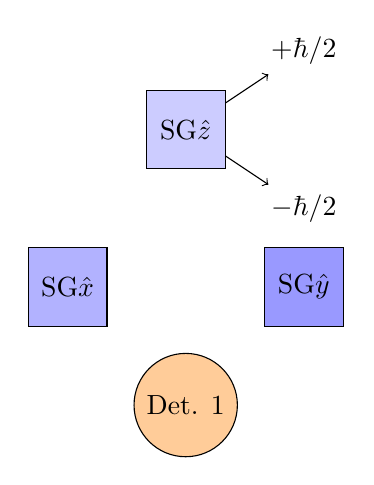
\begin{tikzpicture}
\node[fill=blue!20,shape=rectangle,draw,minimum size=1cm](z) at (0,2){SG$\hat{z}$};
\node (o1) at (1.5,3) {$+\hbar/2$};
\node (o2) at (1.5,1){$-\hbar/2$};
\draw[->] (z) -- (o1);
\draw[->] (z) -- (o2);
\node[fill=blue!30,shape=rectangle,draw,minimum size=1cm] at (-1.5,0){SG$\hat{x}$};
\node[fill=blue!40,shape=rectangle,draw,minimum size=1cm] at (1.5,0){SG$\hat{y}$};
\node[fill=orange!40,shape=circle,draw](D1) at (0,-1.5){Det. $1$};
\end{tikzpicture}
\end{marginfigure}
We can do this for the other two states, too \arnote{Go back to Section~\ref{sec:ybasis} and do this.}, writing $\ket{i}$ and $\ket{o}$ in terms of the $z$ basis vectors:
\bas
\ket{i} =& \frac{1}{\stwo}\ket{u} + \frac{\I}{\stwo}\ket{d}\\
\ket{o} =& \frac{1}{\stwo}\ket{u} - \frac{\I}{\stwo}\ket{d}.
\eas
For simplicity in drawing our experiments, we'll start drawing the magnetic field gradient zone as a simple box with the orientation of the field gradient on it. We use the shorthand ``SG'' to denote a Stern-Gerlach experiment. We can now link together multiple magnetic field gradient zones easily. We'll also label the detector as ``Det.'' We will model the upwards output as being the $+\hbar/2$ spin and the bottom as the $-\hbar/2$ output.

\begin{exercise}
\label{threeSGs}
Consider the following three experiments. You can simulate the outcome of the experiments using a Java \marginnote{I know Java has problems. Find a computer that will run the simulation. Ack.} simulator found at \href{http://www.physics.oregonstate.edu/~mcintyre/ph425/spins/index.html}{Oregon State's PHY425 Page.} Run the simulations and print the results. I want the total number of events and the fraction of events at each output port. \marginnote{\texttt{www.physics.oregonstate.edu/ $\sim$mcintyre/ph425/ spins/index.html}}

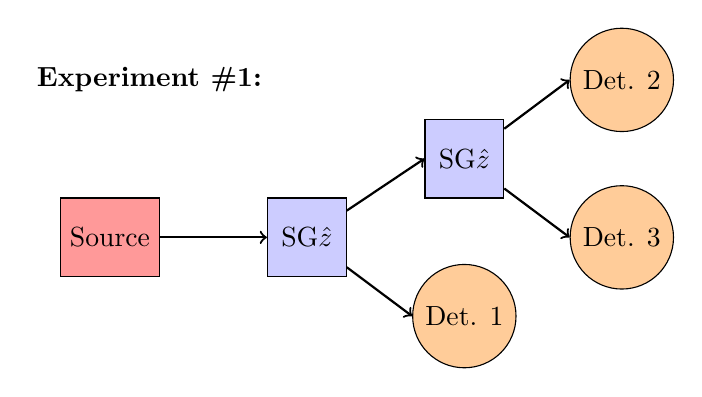
\begin{tikzpicture}
\node at (0,2) {\bf Experiment \#1:};
\node[fill=red!40,shape=rectangle,draw,minimum size=1cm](S) at (-0.5,0){Source};
\node[fill=blue!20,shape=rectangle,draw,minimum size=1cm](SG1) at (2,0){SG$\hat{z}$};
\draw[->,thick] (S) -- (SG1);
\node[fill=blue!20,shape=rectangle,draw,minimum size=1cm](SG2) at (4,1){SG$\hat{z}$};
\draw[->,thick] (SG1) -- (SG2.west);
\node[fill=orange!40,shape=circle,draw](D1) at (4,-1){Det. $1$};
\draw[->,thick] (SG1) -- (D1.west);
\node[fill=orange!40,shape=circle,draw](D2) at (6,2){Det. $2$};
\node[fill=orange!40,shape=circle,draw](D3) at (6,0){Det. $3$};
\draw[->,thick] (SG2) -- (D2.west);
\draw[->,thick] (SG2) -- (D3.west);
\end{tikzpicture}

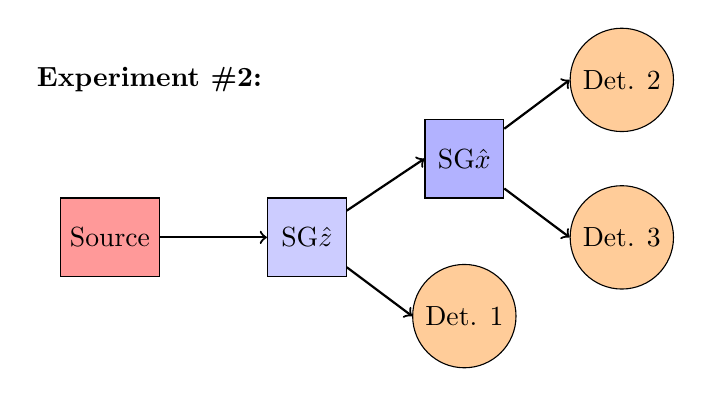
\begin{tikzpicture}
\node at (0,2) {\bf Experiment \#2:};
\node[fill=red!40,shape=rectangle,draw,minimum size=1cm](S) at (-0.5,0){Source};
\node[fill=blue!20,shape=rectangle,draw,minimum size=1cm](SG1) at (2,0){SG$\hat{z}$};
\draw[->,thick] (S) -- (SG1);
\node[fill=blue!30,shape=rectangle,draw,minimum size=1cm](SG2) at (4,1){SG$\hat{x}$};
\draw[->,thick] (SG1) -- (SG2.west);
\node[fill=orange!40,shape=circle,draw](D1) at (4,-1){Det. $1$};
\draw[->,thick] (SG1) -- (D1.west);
\node[fill=orange!40,shape=circle,draw](D2) at (6,2){Det. $2$};
\node[fill=orange!40,shape=circle,draw](D3) at (6,0){Det. $3$};
\draw[->,thick] (SG2) -- (D2.west);
\draw[->,thick] (SG2) -- (D3.west);
\end{tikzpicture}

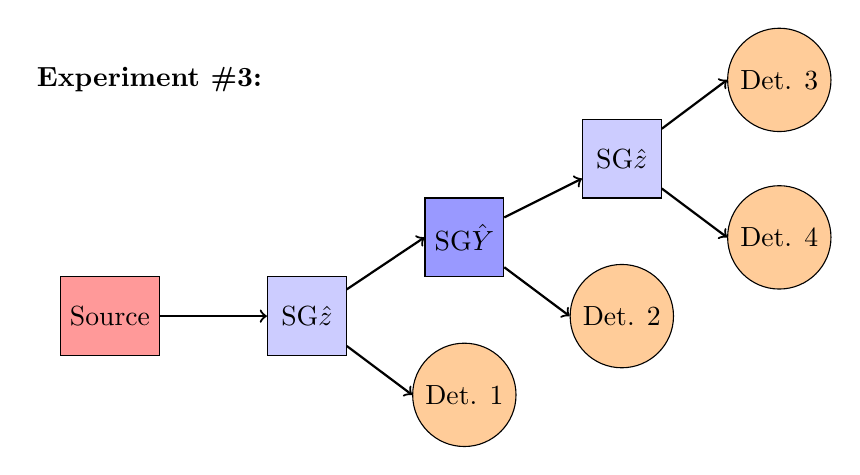
\begin{tikzpicture}
\node at (0,3) {\bf Experiment \#3:};
\node[fill=red!40,shape=rectangle,draw,minimum size=1cm](S) at (-0.5,0){Source};
\node[fill=blue!20,shape=rectangle,draw,minimum size=1cm](SG1) at (2,0){SG$\hat{z}$};
\draw[->,thick] (S) -- (SG1);

\node[fill=blue!40,shape=rectangle,draw,minimum size=1cm](SG2) at (4,1){SG$\hat{Y}$};
\draw[->,thick] (SG1) -- (SG2.west);
\node[fill=orange!40,shape=circle,draw](D1) at (4,-1){Det. $1$};
\draw[->,thick] (SG1) -- (D1.west);


\node[fill=blue!20,shape=rectangle,draw,minimum size=1cm](SG3) at (6,2){SG$\hat{z}$};
\draw[->,thick] (SG2) -- (SG3);
\node[fill=orange!40,shape=circle,draw](D2) at (6,0){Det. $2$};
\draw[->,thick] (SG2) -- (D2.west);

\node[fill=orange!40,shape=circle,draw](D3) at (8,3){Det. $3$};
\draw[->,thick] (SG3) -- (D3.west);
\node[fill=orange!40,shape=circle,draw](D4) at (8,1){Det. $4$};
\draw[->,thick] (SG3) -- (D4.west);
\end{tikzpicture}

\end{exercise}

\begin{example}
Design an ElMaW version of {\bf Experiment \#3} from Exercise \ref{threeSGs}. Sketch where you would need to put all of the optical components to make the equivalent quantum experiment.

\model We will model the ElMaW, beamsplitters, waveplates, and detectors as ideal. From what we've seen before, the spin $z$-basis maps to the ElMaW $V-H$ basis. So the spin $y$-basis must map to the $C_R-C_L$ basis for the ElMaW model.

\vis The layout for the ElMaW is shown in figure~\ref{fig:elmaw_ex3}.
\begin{figure}
\centering
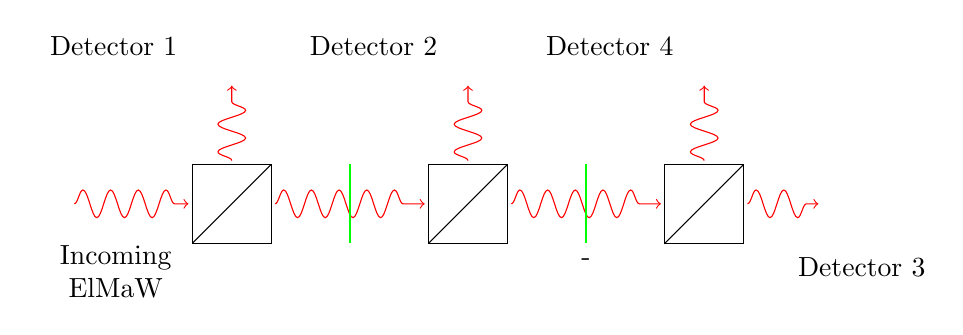
\begin{tikzpicture}


%incoming beam
\draw[red,->,decorate, decoration={snake,amplitude=5,segment length=10, post length=.1cm}](-2,0)--(-.55,0) node[midway, below,shift=({-.2cm,-.4cm}),text width=2cm,black,align=center]{Incoming ElMaW};

%PBS
\draw (-0.5,-.5) rectangle +(1,1);
\draw (-.5,-.5) -- (.5,.5);

%outgoing beam to 1
\draw[red,->,decorate, decoration={snake,amplitude=5,segment length=10, post length=.1cm}](.55,0)--(2.45,0);

\draw[red,->,decorate, decoration={snake,amplitude=5,segment length=10, post length=.1cm}](0,.55)--(0,1.50);
\detector{0.8}{0}{2.0}{90}
\node at (-1.5,2.0) {Detector 1};

\draw[thick,green] (1.5,.5) node[above,black] {\qwp} -- (1.5,-.5);

\draw (2.5,-.5) rectangle +(1,1);
\draw (2.5,-.5) -- (3.5,.5);
\draw[red,->,decorate, decoration={snake,amplitude=5,segment length=10, post length=.1cm}](3.55,0)--(5.45,0);
\draw[thick,green] (4.5,.5)  -- (4.5,-.5)node[below,black] {-\qwp};

\draw[red,->,decorate, decoration={snake,amplitude=5,segment length=10, post length=.1cm}](3,.55)--(3,1.50);
\detector{0.8}{3.8}{2.0}{90}
\node at (1.8,2.0) {Detector 2};

\draw (5.5,-.5) rectangle +(1,1);
\draw (5.5,-.5) -- (6.5,.5);
\draw[red,->,decorate, decoration={snake,amplitude=5,segment length=10, post length=.1cm}](6.55,0)--(7.45,0);

\detector{0.8}{9.4}{0}{0}
\node at (8,-.8) {Detector 3};

\draw[red,->,decorate, decoration={snake,amplitude=5,segment length=10, post length=.1cm}](6,.55)--(6,1.50);
\detector{0.8}{7.5}{2.0}{90}
\node at (4.8,2.0) {Detector 4};

\end{tikzpicture}
\caption[][2cm]{ }
\label{fig:elmaw_ex3}
\end{figure}

\end{example}

Although we have discussed how we measure the probability of getting a particular result (using the Eq.~(\ref{eq:prob})) \marginnote{\ref{tool:prob}}, we haven't addressed how to measure the spin state of our atoms. We need to add another set of tools to our toolbox in order to do this.

\section{The Bloch Sphere}



There is another way to represent the spin basis. The $x,y,z$ notation we have been using is similar to a 3-vector, so we will implement a graphical representation of the quantum state using a 3-vector called the {\em Bloch} vector. We map the quantum states onto a 3-dimensional space in the following way:
\begin{marginfigure}

\centering
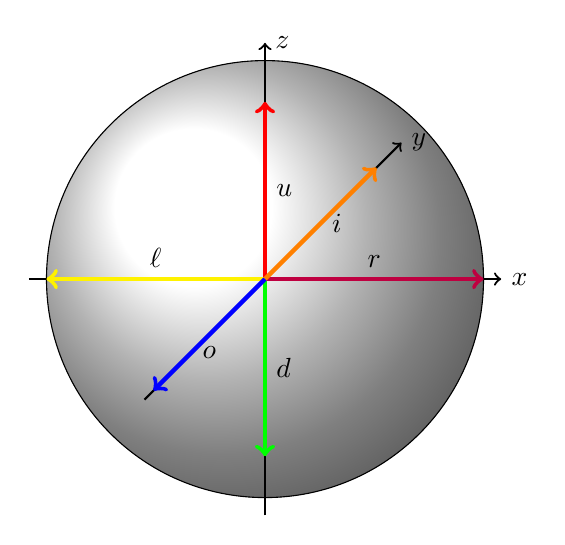
\begin{tikzpicture}[scale=0.75]

\def\R{3.7} % sphere radius
\def\angEl{35} % elevation angle
\filldraw[ball color=white] (0,0) circle (\R);
\foreach \t in {-80,-40,...,80} { \DrawLatitudeCircle[\R]{\t} }
\foreach \t in {-5,-55,...,-175} { \DrawLongitudeCircle[\R]{\t} }

\draw[->,thick](-4,0,0) -- (4,0,0)node[right]{$x$};
\draw[->,thick](0,-4,0) -- (0,4,0)node[right]{$z$};
\draw[->,thick](0,0,5.3) -- (0,0,-6)node[right]{$y$};

\draw[->,red,ultra thick](0,0,0)--(0,3,0) node[right,midway,black]{$\ket{u}$};
\draw[->,green,ultra thick](0,0,0)--(0,-3,0) node[right,midway,black]{$\ket{d}$};

\draw[->,purple,ultra thick](0,0,0)--(3.7,0,0) node[above,midway,black]{$\ket{r}$};
\draw[->,yellow,ultra thick](0,0,0)--(-3.7,0,0) node[above,midway,black]{$\ket{\ell}$};

\draw[->,orange,ultra thick](0,0,0)--(0,0,-4.9) node[right,midway,black]{$\ket{i}$};
\draw[->,blue,ultra thick](0,0,0)--(0,0,4.9) node[below,midway,black]{$\ket{o}$};

\end{tikzpicture}
\caption{The Bloch vector, represented as a unit vector on the Bloch sphere. }
\label{fig:blochsphere}
\end{marginfigure}%
\bas
\ket{u} & \rightarrow  +\hat{z} & \ket{r} & \rightarrow  +\hat{x}  & \ket{i} & \rightarrow  +\hat{y} \\
\ket{d} & \rightarrow  -\hat{z} & \ket{\ell} & \rightarrow  -\hat{x}  & \ket{o} & \rightarrow  -\hat{y} .
\eas
We represent this graphically using 3-vectors as shown in Figure~\ref{fig:blochsphere}. Do not confuse the representation of the quantum state as a Bloch vector with the 3-vectors. They behave in similar ways, but do not mean the same thing. For example, the length of the Bloch vector represents the total probability, so it will typically have a unit length. We can represent any arbitrary quantum state as a unit vector on the Bloch sphere. We have two free parameters to assign: we will use the polar angles $\theta$ (from the $\ket{u}$ vector) and $\phi$ (from the $\ket{r}$ vector), shown in Fig.~\ref{fig:blochangles}. An arbitrary quantum state is then written
\beq
\ket{A} = \cos{\frac{\theta}{2}}\ket{u} + \E{\I\phi} \sin{\frac{\theta}{2}}\ket{d}.
\eeq
\begin{marginfigure}
\centering
\begin{tikzpicture}[scale=1.3]
\draw[->,ultra thick,orange](0,0,0) -- (2,0,0)node[right,black]{$\ket{i}$};
\draw[->,ultra thick,red](0,0,0) -- (0,2,0)node[right,black]{$\ket{u}$};
\draw[->,ultra thick,purple](0,0,0) -- (0,0,2)node[right,black]{$\ket{r}$};
\draw[->,thick](0,0,0) -- (1.5,1,0.8)node[above]{$\ket{A}$};
\draw[dashed] (0,0,0) -- (1.5,0,.8);
\begin{scope}[rotate around={30:(0,0)}]
    \draw (0:0.5) arc (0:62:0.5)node[midway,above]{$\theta$};
\end{scope}

\begin{scope}[canvas is xz plane at y=0, rotate around={90:(0,0)}]
    \draw (0:0.5) arc (0:-62:0.5)node[midway,below]{$\phi$};
\end{scope}

\draw[dashed] (1.5,1,0.8) -- (1.5,0,.8);
\draw[dashed] (0,0,.8) -- (1.5,0,.8);
\draw[dashed] (1.5,0,0) -- (1.5,0,.8);
%\draw[dashed](1.5,1,.8) -- (2,1.33,1.1);
\end{tikzpicture}
\caption{Bloch angles}
\label{fig:blochangles}
\end{marginfigure}%
\begin{exercise}
Find the angles $\theta$ and $\phi$ needed to reproduce all three pairs of basis vectors for the quantum spin state.
\end{exercise}


\chapter{Quantum Operators}

We model the things we measure in our experiment with {\em linear operators}.\marginnote{These of often called ``observables'' because we could, in principle, observe them even if making the actual measurement is challenging.} We start with a general description of the operators and then we will apply them to our quantum state model.

\section{Linear Operators}
A linear operator is something of a machine that acts on quantum states and then returns quantum states:
\marginnote{We will use a ``hat'' $\hat{\;}$ on top of a capital letter ($\hat{M}$ for ``machine'') to denote a linear operator. This will keep it different from a unit vector.}
\beq
\hat{M}\ket{A} = \ket{B}.
\label{eq:linop}
\eeq
In order for our operator to be linear we want the following properties (where $z$ is a complex number):
\bas
\hat{M}z\ket{A} &= z\ket{B} \rmt{ and}\\
\hat{M}\left(\ket{A} + \ket{B}\right) &= \hat{M}\ket{A} + \hat{M}\ket{B}.
\eas

If we have a set of basis vectors like $\ket{j}$, we decompose our quantum states in terms of these vectors. We can then get what the operator $\hat{M}$ looks like in that particular basis. We start with\marginnote{Using \ref{tool:decom}}
\beq
\ket{A} = \sum_j \alpha_j\ket{j} \rmt{ and } \ket{B} = \sum_j \beta_j \ket{j}.
\eeq
We apply this to Eq.~(\ref{eq:linop}) to get
\beq
\sum_j \alpha_j \hat{M}\ket{j} = \sum_j \beta_j \ket{j}.
\eeq
We then multiply both sides by $\bra{k}$ and use the orthogonality relationship \marginnote{Our \ref{tool:orthog} tool} on the right-hand side to get
\beq
\sum_j \alpha_j \bra{k}\hat{M}\ket{j} = \beta_k.
\eeq
This means that, in the $\ket{j}$ basis, our operator is represented by 
\beq
\bra{k}\hat{M}\ket{j} \equiv m_{kj}\, ,
\label{eq:linopel}
\eeq
where we use the shorthand $m_{kj}$ to denote the elements of the $\hat{M}$ operator in this basis. So our linear operator represented in the $\ket{j}$ basis is
\beq
\sum_j m_{kj} \alpha_j = \beta_k,
\eeq
which looks a lot like matrix multiplication.


\subsection{Matrix Representation}
Just like we represented state vectors with column and row matrices, we form a representation of the operator using an $N$ by $N$ matrix, where $N$ is the number of free parameters in the state space. \marginnote{We also call $N$ the size of the Hilbert space. We will eventually find infinite-dimensional Hilbert spaces, but the same ideas apply.} So a matrix representation in a space with three free parameters would look like this:
\beq
\hat{M} \Meq
\begin{pmatrix} m_{11} & m_{12} & m_{13} \\
m_{21} & m_{22} & m_{23} \\
m_{31} & m_{32} & m_{33} \\
\end{pmatrix}.
\eeq
In this representation, our operator acting on our state vectors (Eq.~(\ref{eq:linop})) looks like this:
\beq
\begin{pmatrix} m_{11} & m_{12} & m_{13} \\
m_{21} & m_{22} & m_{23} \\
m_{31} & m_{32} & m_{33} \\
\end{pmatrix} 
\begin{pmatrix} \alpha_{1} \\
\alpha_{2} \\
\alpha_{3}\\
\end{pmatrix} = 
\begin{pmatrix} \beta_{1} \\
\beta_{2} \\
\beta_{3}\\
\end{pmatrix}
\eeq
\begin{example}
What is the outcome of the operator $\hat{M}$ acting on the state $\ket{A}$ in the $\ket{j}$ basis?

\model We model the operator and the quantum state vectors as matrices. We'll use matrix multiplication to get the output.

\vis Visualizing a matrix is tough. But one nice approach is the one by \href{http://people.cornellcollege.edu/dsherman/visualize-matrix.html}{Cornell College} where the matrix deforms the initial state into a new state. \marginnote{\texttt{people.cornellcollege.edu/dsherman/ visualize-matrix.html}}
\begin{figure}
\centering
\includegraphics[width=8cm]{Mxy02yx02.png}
\end{figure}

\sol Our solution uses the rules of matrix multiplication to find the output.
\beq
\begin{pmatrix} m_{11} & m_{12} & m_{13} \\
m_{21} & m_{22} & m_{23} \\
m_{31} & m_{32} & m_{33} 
\end{pmatrix} 
\begin{pmatrix} \alpha_{1} \\
\alpha_{2} \\
\alpha_{3}
\end{pmatrix} = 
\begin{pmatrix} m_{11}\alpha_1+ m_{12}\alpha_2 +m_{13}\alpha_3  \\
m_{21}\alpha_1+ m_{22}\alpha_2 +m_{23}\alpha_3 \\
m_{31}\alpha_1+ m_{32}\alpha_2 +m_{33}\alpha_3
\end{pmatrix}.
\eeq

\assess Our output is a new ket vector as expected.

\end{example}

\section{Linear Operators acting on bra-vectors}

We need to know how linear operators act on bra vectors, too. We want something like
\beq
\bra{A}\hat{M}.
\eeq
So how are $\hat{M}\ket{A}=\ket{B}$ and $\bra{A}\hat{M}=\bra{B}$ related to each other? If we do this in component form (in the $\ket{j}$ basis), we get
\beq
\sum_j m_{kj} \alpha_j = \beta_k
\eeq
and
\beq
\sum_j m_{jk}^* \alpha_j^* = \beta_k^*.
\eeq
There are two differences between these two relationships:
\begin{enumerate}
\item We take the complex conjugate of each of the matrix entries.
\item We flip the location of the indices on each of the $m_{kj}$ entries. \marginnote{Also known as taking the transpose of the matrix.}
\end{enumerate}
Put these two together and we get the complex conjugate-transpose also known as the {\em Hermitian conjugate}. This is defined as
\beq
\left(\hat{M}^T\right)^* = \hat{M}^\dagger.
\eeq

\begin{exercise}
What is the Hermitian conjugate of this operator in the matrix representation?
\beq\hat{M}\Meq
\begin{pmatrix} \frac{1}{3} & 2+\I & \E{3\I\pi/2} \\
-4+2\I & \frac{2}{3} & 6 \\
\E{\I\pi/\sqrt{2}} & 9 & \frac{-1}{3}
\end{pmatrix} 
\eeq
\end{exercise}

\section{Operator Eigenvalues and Eigenvectors}
If a general linear operator transforms one ket vector into another ket vector, there is a special type of operator and related ket vector such that when the operator acts on the ket vector, it only scales the ket vector by some number. This special ket vector, known as the {\em eigenvector}, is otherwised unchanged. The scale factor is known as the {\em eigenvalue}. In symbolic terms we have\marginnote[-1cm]{This notation is awkward, but common. We have a ket vector in some basis $\ket{\lambda}$ and its eigenvalue $\lambda$ which is just a (complex) number.} 
\beq
\hat{L}\ket{\lambda} = \lambda\ket{\lambda}.
\label{eq:eigen}
\eeq\toolnote{\toollabel{tool:eigen}{\includegraphics{tool6.tikz} {\bf Eigenvaluator}}  This tool is used to evaluate the operation of a linear operator on one of its eigenvectors. It returns the eigenvalue and the eigenvector.} 
Let me give you a feel for how this works.
\begin{example}
Show that, in the matrix representation, $\ket{\lambda_1}\Meq\vket{1}{1}$ is an eigenvector of $\hat{M}\Meq\begin{pmatrix}1&2\\2&1\end{pmatrix}$.

\model It makes sense to use the matrix representation for our quantum states. We don't know much else about the system.

\vis This would be akin to multiplying a vector by some number or rotating a vector about is own axis. Hard to visualize.

\sol We run the operation $\hat{M}\ket{\lambda_1}$ and get $\vket{3}{3} \rightarrow 3 \ket{\lambda_1}$. That makes $\lambda_1=3$ and we have an eigenvalue and an eigenvector.\arnote{Work out this matrix multiplication in your notes.}

\assess We got a column vector from the operator acting on the column vector. That's what we expect.

\end{example}

\begin{exercise}
Check if $\vket{1}{0}$ and $\vket{1}{-1}$ are also eigenvectors of $\hat{M}\Meq\begin{pmatrix}1&2\\2&1\end{pmatrix}$. If they are, what are their eigenvalues?

\end{exercise}

\section{Hermitian Operators}
There is a special subset of linear operators that are equal to their own Hermitian conjugates:
\beq
\hat{M}^\dagger = \hat{M}.
\eeq%
We are particularly interested in this type of operator, called a {\em Hermitian Operator}, because of three properties:
\begin{enumerate}
\item The eigenvalues of a Hermitian operator are real numbers. This is good --- we will be identifying these as the outcomes of measurements and we only want real numbers for things we measure.
\item The eigenvectors of a Hermitian operator are a complete set. Any arbitrary ket-vector can be decomposed using our tools into the basis of eigenvectors.
\item The eigenvectors of a Hermitian operator can be made into an orthonormal set with unique eigenvalues. \marginnote[-1cm]{There are times when there are degenerate eigenvalues and a bit of work has to be done to get there, but we'll mostly be avoiding that situation in this Guide.}
\end{enumerate}

In the next example, we'll work through why it is that being a Hermitian operator means that the eigenvalues are real.
\begin{example}
Show that a Hermitian operator has real eigenvalues.

\model We model our quantum state as a ket-vector and our operator as Hermitian.

\vis Not much to show here--- but I'm thinking about it.

\sol Since $\hat{M}\ket{\lambda}=\lambda\ket{\lambda}$, we can flip this to the bra-vector version: $\bra{\lambda}\hat{M}^\dagger=\bra{\lambda}\lambda^*$. But since $\hat{M}^\dagger = \hat{M}$ (the definition of a Hermitian operator), that means that $\bra{\lambda}\hat{M}=\bra{\lambda}\lambda^*$.

Now we multiply the first piece by $\bra{\lambda}$ and the second by $\ket{\lambda}$ and get
\bas
\bra{\lambda}\hat{M}\ket{\lambda} &= \lambda\avg{\lambda|\lambda}\\
\bra{\lambda}\hat{M}\ket{\lambda} &= \lambda^*\avg{\lambda|\lambda}.
\eas
We subtract these two and get $\lambda - \lambda^*=0$ which is only valid if $\lambda$ is a real number.

\assess We got a general solution without having to use specific values.

\end{example}

\begin{exercise}
Show that if a Hermitian operator has two unique eigenvalues, the corresponding eigenvectors must be orthogonal.
\end{exercise}

\section{Spin Operators}
\label{sec:spinop}
\begin{marginfigure}\centering
\begin{tikzpicture}
\node[fill=blue!20,shape=rectangle,draw,minimum size=1cm](z) at (0,3){SG$\hat{z}$};
\node (o1) at (1.5,3) {$\hat{S}_z$};
\draw[->] (z) -- (o1);

\node[fill=blue!30,shape=rectangle,draw,minimum size=1cm](x) at (0,1.5){SG$\hat{x}$};
\node (o2) at (1.5,1.5) {$\hat{S}_x$};
\draw[->] (x) -- (o2);
\node[fill=blue!40,shape=rectangle,draw,minimum size=1cm](y) at (0,0){SG$\hat{y}$};
\node (o3) at (1.5,0) {$\hat{S}_y$};
\draw[->] (y) -- (o3);
\end{tikzpicture}
\end{marginfigure}


We wrap up this section by connecting Hermitian operators to our quantum spin model. We will now model the Stern-Gerlach magnetic field gradient as a Hermitian operator. Now the process of sending an atom through the magnetic field gradient becomes an operator acting on a quantum state. We will represent $\hat{S}_z$ as the matrix (in the $z$ basis)
\beq
\hat{S}_z \Meq \frac{\hbar}{2}\szmatrix .
\eeq
\begin{example}
What is the output state from the SG$\hat{z}$ if we sent in the state $\ket{u}$?

\model We model the SG magnetic field gradient as an operator in the $z$ basis. We will work in the matrix representation where $\ket{u} \Meq \vket{1}{0}$.

\vis 
\begin{figure}
\centering
\begin{tikzpicture}
\node(inputnd) at (-2,0){$\ket{u}$};
\node[fill=blue!20,shape=rectangle,draw,minimum size=1cm](zor) at (0,0){SG$\hat{z}$};
\draw[->] (inputnd) -- (zor);
\node (o1) at (1.5,1) {$+\hbar/2$};
\node (o2) at (1.5,-1){$-\hbar/2$};
\draw[->] (zor) -- (o1);
\draw[->] (zor) -- (o2);

\end{tikzpicture}
\end{figure}


\sol We want
\beq
\hat{S}_z\ket{u} \Meq \frac{\hbar}{2}\szmatrix\vket{1}{0}=\frac{\hbar}{2}\vket{1}{0}.
\eeq

So the output is the state $\hbar/2\ket{u}$. 

\assess This shows that $\ket{u}$ is an eigenvector of $\hat{S}_z$ as we expected with eigenvalue of $\hbar/2$.


\end{example}

We do the same thing with the other two directions, $x$ and $y$. We will write these operators in the same $z$ basis, though. That means when we want to use them, we have to write any input vector in the $z$-basis (in terms of $\ket{u}$ and $\ket{d}$).
\beq
\begin{split}
\hat{S}_z &\Meq \frac{\hbar}{2}\szmatrix\\
\hat{S}_x &\Meq \frac{\hbar}{2}\sxmatrix\\
\hat{S}_y &\Meq \frac{\hbar}{2}\symatrix 
\end{split}
\label{eq:sspins}
\eeq

\begin{exercise}
What is the output state if we send $\ket{\ell}$ into the $SG_x$ Stern-Gerlach experiment? How about if  $\ket{o}$ is sent into the $SG_y$?
\end{exercise}

\chapter{Quantum Mechanic's Model}

We now put everything together into a model to describe  both the ElMaW/Beamsplitter and the Stern-Gerlach experiments. 

\section{The Quantum Model}
Here's how the model works:
\begin{enumerate}
\item Measurable physical quantities are modeled as Hermitian operators $\hat{L}$ (where $\hat{L}^\dagger=\hat{L}$).
\item The results of a measurement is one of the eigenvalues of $\hat{L}$ called $\lambda_j$ where $\ket{\lambda_j}$ are the orthogonal eigenvectors of $\hat{L}$.
\item If we measure value $\lambda_j$, then the output state of the system is now $\ket{\lambda_j}$.
\item If $\ket{\Psi_\rmt{in}}$ is the state-vector input of a system, the probability of measuring value $\lambda_j$ is 
\beq
P(\lambda_j) = \abs{\avg{\lambda_j|\Psi_\rmt{in}}}^2 \mathnote{Using \ref{tool:prob}}. 
\eeq
\end{enumerate}



\section{Average Measurements}
\marginnote[-0.5cm]{Although this is often called an ``expectation value'', that is an awful name. There are many cases for which the most likely value and the average value are not the same.}
It is often useful to ask what we would get if we repeated a measurement many times and then took the average of all the results. We can evaluate this with our model using the following notation:\toolnote[0.2cm]{\toollabel{tool:avg}{\includegraphics{tool5.tikz} {\bf Expectation Evaluator}}  This tool is used to find the average measurement value of an operator for an input state.} 
\beq
\avg{\hat{L}} = \bra{\Psi_\rmt{in}}\hat{L}\ket{\Psi_\rmt{in}}.
\label{eq:avg}
\eeq
Let's practice using this tool.
\begin{example}
An atom is prepared in the spin state $\ket{\Psi}=\ket{u}.$ What is the average measurement if the atom is sent through the SG$\hat{z}$ magnetic field gradient?

\model We model the atom as a quantum state and the SG magnetic field gradient as the Hermitian operator $\hat{S}_z$. We will work in the $z$ basis where $\ket{u} \Meq\vket{1}{0}$.

\vis
\begin{figure}
\centering
\begin{tikzpicture}
\node(inputnd) at (-2,0){$\ket{u}$};
\node[fill=blue!20,shape=rectangle,draw,minimum size=1cm](zor) at (0,0){SG$\hat{z}$};
\draw[->] (inputnd) -- (zor);
\node (o1) at (1.5,1) {$+\hbar/2$};
\node (o2) at (1.5,-1){$-\hbar/2$};
\draw[->] (zor) -- (o1);
\draw[->] (zor) -- (o2);

\end{tikzpicture}
\end{figure}

\sol We use Eq.~(\ref{eq:avg}) \marginnote{\ref{tool:avg}} to calculate the average measurement. In the matrix representation, this becomes
\beq
\bra{u}\hat{S}_z\ket{u}\Meq \vbra{1}{0}\frac{\hbar}{2}\szmatrix\vket{1}{0}.
\eeq
Performing the matrix multiplication gives us $\hbar/2$. 

\assess That agrees with our experimental results. What is the probability of measuring $\ket{u}$? We find that $P(\ket{u}) = \abs{\avg{u|\Psi}}^2=1$.\marginnote{Using \ref{tool:prob}} After the measurement the state is still $\ket{u}$.

\end{example}

\begin{exercise}
An atom is prepared in the spin state $\ket{\Psi}=\ket{r}.$ 
\begin{enumerate}
\item What is the average measurement if the atom is sent through the SG$\hat{z}$ magnetic field gradient?
\item What is the probability of measuring $\hbar/2$ in a single experiment? 
\item What is the state after measurement if we measure $\hbar/2$?
\end{enumerate}
\end{exercise}

We model our ElMaW system using the same tools. We model the \hwp, \qwp, and PBS system using the following set of operators. If we write them all in the $V-H$ basis, we get:
\bas
(\lambda/2 = 0^\circ, \lambda/4=0^\circ )\equiv\hat{\sigma}_3&\Meq \szmatrix \\
(\lambda/2 = -45^\circ, \lambda/4=0^\circ ) \equiv\hat{\sigma}_1&\Meq \sxmatrix \\
(\lambda/2 = 0^\circ, \lambda/4=45^\circ )\equiv\hat{\sigma}_2&\Meq \symatrix .
\eas
The eigenvalues of each operator are the polarization states we've used before:
\bas
\hat{\sigma}_3\ket{V} & = +1 \ket{V}\mathnote{Using \ref{tool:eigen}}\\
\hat{\sigma}_3\ket{H} & = -1 \ket{H}.
\eas

We'll practice using this system, too.

\begin{example} 

We send the ElMaW from a single atom through a $V$ polarizer. What is the average measurement if the \hwp is set at ${-45}^\circ$?

\model We are given a state prepared in the $V-H$ basis, but since the \hwp is set at ${-45}^\circ$ and the \qwp is set at $0^\circ$, we need to measure in the $D_R-D_L$ basis. We will model the PBS in this basis and write our input state in that basis, too.

\vis 
\begin{figure}
\centering
\begin{tikzpicture}[scale=0.6]
\draw (-0.5,-.5) rectangle +(1,1) node[below,shift={(-.2,-.6)}]{PBS};
\draw (-.5,-.5) -- (.5,.5);
\draw[red,->,decorate, decoration={snake,amplitude=5,segment length=10, post length=.1cm}](-3.3,0)--(-.55,0) node[midway, above,shift=({0,.2cm})]{};
\draw[red,->,decorate, decoration={snake,amplitude=5,segment length=10, post length=.1cm}](.55,0)--(2,0);
\detector{1}{2.1}{0}{0}
\node at (2.5,-.8) {Detector 1};
\draw[red,->,decorate, decoration={snake,amplitude=5,segment length=10, post length=.1cm}](0,.55)--(0,2);
\detector{1}{0}{2.1}{90}
\node at (1.6,2.8) {Detector 2};
\fill[red] (-5,0) circle(0.1);
\draw[red,decorate,decoration={expanding waves,angle=35}](-5,0) -- (-3.5,0);
\draw[thick] (-3.5,.2) -- (-3.5,2);
\draw[thick] (-3.5,-.2) -- (-3.5,-2);
\draw[thick,green] (-2.5,-1) node[below,black,text width=1.5cm, align=left,shift={(.4,-.1)}] {\hwp at ${-45}^\circ$} -- (-2.5,1);
\draw[thick,blue] (-1.5,-1) -- (-1.5,1) node[above,shift={(-0.5,.3)},text width=2cm, align=right,black] {\qwp at $0^\circ$};
\end{tikzpicture}
\end{figure}

\sol We will use the eigenvalue relationships to find the average measurement. We need to write our initial state in the  $D_R-D_L$ basis:
\beq
\ket{\Psi} =\frac{1}{\stwo}\ket{D_R} + \frac{1}{\stwo}\ket{D_L}.\mathnote{\ref{tool:decom}}
\eeq
Now we want $\bra{\Psi}\hat{\sigma}_1\ket{\Psi}$. We do the right-hand part and get
\beq
\bra{\Psi}\left(\hat{\sigma}_1\ket{\Psi}\right) = \bra{\Psi}\hat{\sigma}_1\left(\frac{1}{\stwo}\ket{D_R} + \frac{1}{\stwo}\ket{D_L}\right)
\eeq
Now we use the eigenvalue relationships since $\ket{D_R}$ and $\ket{D_L}$ are both eigenvectors of $\hat{\sigma}_1$.
\beq
\bra{\Psi}\left(\hat{\sigma}_1\ket{\Psi}\right) = \bra{\Psi}\left((+1)\frac{1}{\stwo}\ket{D_R} + (-1)\frac{1}{\stwo}\ket{D_L}\right)\mathnote{\ref{tool:eigen}}
\eeq

Finally, we expand the bra-vector $\bra{\Psi}$ and use the fact that $\avg{D_R|D_L}=0$\marginnote{\ref{tool:orthog}} to get

\beq
\bra{\Psi}\hat{\sigma}_1\ket{\Psi}=\left((+1)\frac{1}{2} + (-1)\frac{1}{2}\right) = 0.
\eeq\arnote{Be sure to work out the missing steps here.}

\assess This is what we expected for our average measurement. Half the time we get a $+1$, the other half we get $-1$. This averages to zero.

\end{example}

\begin{exercise}
We send the ElMaW from a single atom through a $D_R$ polarizer.
\begin{enumerate}
\item What is the average measurement if the \hwp is set at $0^\circ$ and the \qwp is set at ${45}^\circ$?
\item What is the probability of measuring $-1$ in a single experiment? 
\item What is the state after measurement if we measure $-1$?
\end{enumerate}
\end{exercise}

\section{Averaging in a Specific Basis}
\label{sec:operatormodel4}
 \marginnote[-1cm]{Of course, we need to know the eigenvalues and eigenvectors of the operator to do this. You could use your favorite \CAS to find them for any operator in the matrix representation. \ref{tool:decom}} We can use our tools to figure out the average measurement of an operator $\hat{L}$ if we know we have decomposed the initial state vector $\ket{\Psi}$ in terms of its eigenvectors $\ket{\lambda_j}$.We start by writing 
\beq
\ket{\Psi} = \sum_j \alpha_j \ket{\lambda_j}. 
\eeq%
When we act on this state with the operator, we get
\beq
\hat{L}\ket{\Psi} = \sum_j\alpha_j \hat{L}\ket{\lambda_j} = \sum_j\alpha_j\lambda_j\ket{\lambda_j}.
\eeq%
So we now find the expectation value of $\avg{\hat{L}}$:
\bas
\bra{\Psi}\hat{L}\ket{\Psi} &= \sum_k \alpha_k^* \bra{\lambda_k}\sum_j \alpha_j \lambda_j \ket{\lambda_j}\\
\bra{\Psi}\hat{L}\ket{\Psi} &= \sum_k \alpha_k^* \alpha_k \lambda_k.
\eas\marginnote[-1cm]{\ref{tool:orthog}}%
We now relate this to the probability of making a measurement:
\beq
P(\lambda_j) = \abs{\avg{\lambda_j|\Psi}}^2 = \avg{\Psi|\lambda_j}\avg{\lambda_j|\Psi}\mathnote{\ref{tool:prob}}
\eeq
We now write our initial state in terms of the basis vectors $\ket{\lambda_k}$ and $\ket{\lambda_l}$:\marginnote{\ref{tool:decom}, \ref{tool:orthog}}
\bas
P(\lambda_j) =& \sum_k \alpha_k^* \avg{\lambda_k|\lambda_j} \sum_l \alpha_l \avg{\lambda_j|\lambda_l}\\
=& \alpha_j^* \alpha_j 
\eas%
This means that the average of many measurements can be written in the following compact way:\marginnote{This is the same as \ref{tool:avg} and joins that tool as another useful way of finding the expectation value.}
\beq
\bra{\Psi}\hat{L}\ket{\Psi} = \sum_j P(\lambda_j)\lambda_j.
\label{eq:probtoaverage}
\eeq
This agrees with the notion of an average measurement given a random distribution of outcomes.

\begin{tacticsbox}
\label{tec:expec}
Putting this all together, the general technique is to:
\begin{enumerate}
\item Model the physical system as a linear operator.
\item Determine the eigenvalues and eigenvectors of the operator.
\item Write the input state in the operator's eigenvector basis.
\item Calculate the average value of the measurement of the operator.
\end{enumerate}
\end{tacticsbox}

\begin{example}
What is the average measurement if a $C_R$ polarized wave is measured in the $V-H$ basis?

\model We model the ElMaW as a quantum state with initial state $\ket{C_R}$. We model the measurement system as a quantum operator $\hat{\sigma}_3$. Since we are working in the $V-H$ basis, we want to wite $\ket{C_R}$ in that basis.

\vis 
\begin{figure}
\centering
\begin{tikzpicture}[scale=0.6]
\draw (-0.5,-.5) rectangle +(1,1) node[below,shift={(-.2,-.6)}]{PBS};
\draw (-.5,-.5) -- (.5,.5);
\draw[red,->,decorate, decoration={snake,amplitude=5,segment length=10, post length=.1cm}](-3.3,0)--(-.55,0) node[midway, above,shift=({0,.2cm})]{};
\draw[red,->,decorate, decoration={snake,amplitude=5,segment length=10, post length=.1cm}](.55,0)--(2,0);
\detector{1}{2.1}{0}{0}
\node at (2.5,-.8) {Detector 1};
\draw[red,->,decorate, decoration={snake,amplitude=5,segment length=10, post length=.1cm}](0,.55)--(0,2);
\detector{1}{0}{2.1}{90}
\node at (1.6,2.8) {Detector 2};
\fill[red] (-5,0) circle(0.1);
\draw[red,decorate,decoration={expanding waves,angle=35}](-5,0) -- (-3.5,0);
\draw[thick] (-3.5,.2) -- (-3.5,2);
\draw[thick] (-3.5,-.2) -- (-3.5,-2);
\draw[thick,green] (-2.5,-1) node[below,black,text width=1.5cm, align=left,shift={(.4,-.1)}] {\hwp at $0^\circ$} -- (-2.5,1);
\draw[thick,blue] (-1.5,-1) -- (-1.5,1) node[above,shift={(-0.5,.3)},text width=2cm, align=right,black] {\qwp at $0^\circ$};
\end{tikzpicture}
\end{figure}

\sol We saw previously that $\ket{C_R} =  \frac{1}{\stwo}\ket{V} + \frac{\I}{\stwo}\ket{H}$. So 
\bas
P(+1) =& \abs{\frac{1}{\stwo}}^2  = \frac{1}{2}\\
P(-1) =& \abs{\frac{\I}{\stwo}}^2 = \frac{1}{2}
\eas

So our average measurement will be:
\beq
\bra{C_R}\hat{\sigma}_3\ket{C_R}= \frac{1}{2}(+1) + \frac{1}{2}(-1)=0.
\eeq \arnote{Be sure you know how we got here - work it out on your own.}

\assess This is what we expect should be - there are equal probabilities of measuring $\ket{V}$ and $\ket{H}$
\end{example}

\begin{exercise}
What is the average measurement if an atom has initial spin $\ket{\Psi}=(\sqrt{1/3})\ket{u} + (\sqrt{2/3})\ket{d}$ and is measured through the SG$\hat{y}$ magnetic field gradient?
\end{exercise}

\subsection{Common Misconception}
\begin{marginfigure}\centering
\begin{tikzpicture}[scale=0.6]
\draw (-0.5,-.5) rectangle +(1,1);
\draw (-.5,-.5) -- (.5,.5);
\draw[red,->,decorate, decoration={snake,amplitude=5,segment length=10, post length=.1cm}](-3.3,0)--(-.55,0) node[midway, above,shift=({0,.2cm})]{};
\draw[red,->,decorate, decoration={snake,amplitude=5,segment length=10, post length=.1cm}](.55,0)--(2,0);
\detector{1}{2.1}{0}{0}

\draw[red,->,decorate, decoration={snake,amplitude=5,segment length=10, post length=.1cm}](0,.55)--(0,2);
\detector{1}{0}{2.1}{90}
\draw[thick,green] (-2.5,-1) -- (-2.5,1);
\draw[thick,blue] (-1.5,-1) -- (-1.5,1) ;
\fill[black,opacity=0.3](-3,-1.2) rectangle (1.4,1.4) node[midway,below,black,opacity=1,shift={(0,-0.7)}]{Operator Model};


\begin{scope}[shift={(-3,-4)},scale=1.3]

%atom beam
\fill[color=green!80,thick,decorate, decoration={shape backgrounds, shape=circle,shape size=0.2cm,shape sep={0.4cm, between centers}}](0,0,0) -- (2.4,0,0) ;

\begin{scope}[shift={(2.4,0,0)}]
\fill[color=green!80,thick,decorate, decoration={shape backgrounds, shape=circle,shape size=0.1cm,shape sep={0.4cm, between centers}}](0,0) -- (20:3.0);
\fill[color=green!80,thick,decorate, decoration={shape backgrounds, shape=circle,shape size=0.1cm,shape sep={0.4cm, between centers}}](0,0) -- (-20:3.0);
\end{scope}

%field gradient zone
\begin{scope}[shift={(0,.15,0)}]
\begin{scope}[canvas is xz plane at y=.5,shift={(2,0,0)}]
\fill[blue,opacity=0.5] (-.5,-.5) rectangle +(1,1);
\end{scope}
\begin{scope}[canvas is yz plane at x=2.5]
\fill[blue,opacity=0.4] (-.5,-.5) rectangle +(1,1);

\end{scope}
\begin{scope}[canvas is xy plane at z=.5,shift={(2,0,0)}]
\fill[blue,opacity=0.3] (-.5,-.5) rectangle +(1,1);

\end{scope}

\draw[->,thick](2.5,-.5,-.5)--(2.5,.5,-.5);

\end{scope}


\begin{scope}[canvas is yz plane at x=5]
\fill[orange,opacity=0.4] (-1,-1) rectangle +(2,2);
\end{scope}
%\node[text width=2cm,align=center] at (4.5,-1.1,0) {Atom Position Detector};

\fill[black,opacity=0.3](1,-1) rectangle (3,1)node[midway,below,black,opacity=1,shift={(0,-0.7)}]{Operator Model};


\end{scope}

\end{tikzpicture}
\end{marginfigure}
It is a common misconception that acting with an operator is the same thing as making a measurement with an actual physical system. That isn't how our model works. We can use the operator model to figure out what the {\em average} of many measurements will be. We can use the probability tool to figure out what the probability of any particular measurement will be. We can even say what the measurement value will be and what the resulting state is if we make a particular measurement. But the operator does not model a measurement. It models the interaction system {\em prior to} the measurement devices. We will say more about how to model the actual measurement devices a bit later on.


\section{Non-uniqueness of the Quantum State}
We have addressed this before, but I want to make sure we have hit this concept explicitly. The quantum state is only specified up to an arbitbitrary phase factor $\E{\I \theta}$. This is because all of our normalizations and measurements are based on taking the state vector times its complex conjugate. So if
\beq
\ket{\Psi} = \E{\I\theta}\ket{A},
\eeq
then 
\beq
\avg{\Psi|\Psi} = \bra{A}\E{-\I\theta}\E{\I\theta}\ket{A} = \avg{A|A}.
\eeq
So the phase factor $\theta$ could be anything at all and it won't affect the outcome of the measurement. This can be handy as it will allow us to ignore any overall phases.\marginnote[-3cm]{This is similar to the idea from classical physics that only energy differences matter and not absolute energies. This arbitrary phase factor plays an important role in developing ideas beyond this class.}

\begin{exercise}
You are given a beam of atoms that are all prepared in the intial state
\beq
\ket{\Psi} = \frac{1}{2} \ket{u} + \frac{\sqrt{3}\I}{2}\ket{d}.
\eeq
You are also given a new system that is modeled by the following Hermitian operator:
\beq
\hat{B} = b_0\begin{pmatrix}1&1\\1&1\end{pmatrix}
\eeq
where $b_0$ is a real constant. 
\begin{enumerate}
\item What are the possible outcomes of the measurements? What are the probabilities of getting each?
\item If we make many measurements with this system, what is the average value of the measurements? Calculate this two different ways: using the probabilities from the first part, and using the definition of the average of an operator.
\end{enumerate}

\end{exercise}


\chapter{Part \ref{part1} Summary and Test}

Up to this point we have covered the need for a quantum model to describe two different experiment systems: the ElMaWs from a single trapped atom and the internal spin states of atoms. We developed a mathematical model for describing measurement probabilities and outcomes based on a complex vector space. We developed a set of tools that we used to make specific predictions of the average outcomes of measurements of these systems.

It is important to practice using these tools to model experiments. The following set of exercises is a good way to test your understanding of these models. Try to do these without referring to the previous text. If you can do all of them and your solutions agree with those provided on the following pages, then you are in pretty good shape to move forward with the material. If not, you should specifically review the material  you do not have mastery of yet, then retry the test exercises.

\begin{exercise}
Your research advisor asks you to produce a beam of spin-$1/2$ atoms which are in the state
\beq
\ket{\Psi} = -\frac{1}{\stwo}\ket{u} + \frac{\I}{\stwo}\ket{d}.
\eeq
\begin{enumerate}
\item You measure the state using a Stern-Gerlach apparatus oriented in the $y$-direction. What is the probability of getting a ${-\hbar/2}$ result?
\item What is the state of the atoms after you measure a ${-\hbar/2}$ result?
\item What is the expected average if you prepare many atoms in the same state and then measure them?
\end{enumerate}
\end{exercise}

\begin{exercise}
Consider two measurement propositions about a atomic spin state initially prepared as $\ket{\ell}$:
\begin{enumerate}
\item[Prop. A:] When measured with an SG$\hat{x}$, do we measure ${-\hbar/2}$?
\item[Prop. B:] When measured with an SG$\hat{z}$, do we measure ${-\hbar/2}$?
\end{enumerate}
For which measurement results will these propositions be true? How about A {\bf and} B as well as A {\bf or} B? Consider the reverse as well: B {\bf and} A and B {\bf or} A.
\end{exercise}

\begin{exercise}
Identify the nature (bra, ket, operator, or number) of the following: 
\begin{enumerate}
\item $\avg{\psi|\phi}\hat{A}$
\item $\hat{A}\ket{\psi}\avg{\phi|\psi}$
\item $\hat{B}\ket{\psi}\bra{\phi}\hat{A}\ket{\psi} $ 
\end{enumerate}

Why must the bra and ket  vectors we use be normalized to one?
\end{exercise}

\begin{exercise}
You are given a beam of atoms that are all prepared in the intial state
\beq
\ket{\Psi} = \frac{-2}{\sqrt{7}} \ket{u} + \I \sqrt{\frac{3}{7}}\ket{d}.
\eeq
You are also given a new system that is modeled by the following operator in the $z$-basis:
\beq
\hat{W} \Meq 2\begin{pmatrix}9&0\\0&16\end{pmatrix}
\eeq
\begin{enumerate}
\item Show that $\hat{W}$ is a Hermitian operator. What are the eigenvalues and eigenvectors of the operator.
\item What is the average measurement of $\avg{\hat{W}}$ for the given input state $\ket{\Psi}$?
\end{enumerate}

\end{exercise}

Stop here and don't continue reading until you have completed the exercises.
\newpage
\begin{example}
We model the atom as a quantum state and we model the measurement as the operator $\hat{S}_y$. We first notice that the input state $\ket{\Psi} = -\ket{o}$. This simplifies the problem significantly, since $\ket{o}$ is an eigenvector of the $\hat{S}_y$ operator.

\begin{enumerate}
\item The probability of measuring ${-\hbar}/2$ is just the probability of measuring $\ket{o}$. Since the input state is $\ket{\Psi} = -\ket{o}$, the probability is
\beq
P(\ket{o}) = \abs{\avg{o|\Psi}}^2 = \abs{-1}^2 = 1.
\eeq
\item After measuring ${-\hbar}/2$, the atom is in the state $\ket{o}$, since that is the eignevector of $\hat{S}_y$ with eigenvalue of ${-\hbar}/2$.
\item The average result after making many measurements is just ${-\hbar}/2$, since the probability of making this measurement is $1$.
\end{enumerate}
\end{example}

\begin{example}
We model the two measurements as the quantum operators $\hat{S}_x$ and $\hat{S}_z$. The output of the measurements are:
\bas
\hat{S}_x\ket{\ell} =& \frac{-\hbar}{2}\ket{\ell}\\
\hat{S}_z\ket{\ell} =& \hat{S}_z\left(\frac{1}{\stwo}\ket{u}-\frac{1}{\stwo}\ket{d}\right) = \frac{\hbar}{2}\frac{1}{\stwo}\ket{u} - \left(\frac{-\hbar}{2}\right)\frac{1}{\stwo}\ket{d}.
\eas
Prop. A is true 100\% of the time.
Prop. B is true 50\% of the time since the probability of measuring ${-\hbar}/2$ is 50\%.
The proposition {\bf A or B} is always true since the probability of measuring A is 100\%. The proposition {\bf A and B} can be visualized using our schematic diagram shown in Fig.~\ref{fig:t1}.
\begin{figure}
\centering
\begin{tikzpicture}
\node(inputnd) at (-2,0){$\ket{\ell}$};
\node[fill=blue!20,shape=rectangle,draw,minimum size=1cm](xor) at (0,0){SG$\hat{x}$};
\draw[->] (inputnd) -- (zor);
\node (o1) at (2,1) {$+\hbar/2$ -- 0\% of the time.};
\node[fill=blue!20,shape=rectangle,draw,minimum size=1cm](zor) at (2,-1){SG$\hat{z}$};
\node[text width=2cm] (o2) at (4,-2){$-\hbar/2$ True 50\% of the time.};
\node[text width=2cm] (o3) at (4,0){$+\hbar/2$ False};
\draw[->](xor) -- (o1);
\draw[->](xor) -- (zor) node[below,midway]{True};
\draw[->] (zor) -- (o3);
\draw[->] (zor) -- (o2);
\end{tikzpicture}
\caption[][2cm]{ }
\label{fig:t1}
\end{figure}

So the proposition {\bf A and B} is true 50\% of the time.

We reverse this to look at the other propositions, shown in Fig.~\ref{fig:t2}. This shows that the proposition is true 25\% of the time.
\begin{figure}
\centering
\begin{tikzpicture}
\node(inputnd) at (-2,0){$\ket{\ell}$};
\node[fill=blue!20,shape=rectangle,draw,minimum size=1cm](xor) at (0,0){SG$\hat{z}$};
\draw[->] (inputnd) -- (xor);
\node (o1) at (1.5,1) {$+\hbar/2$ -- 50\% of the time.};
\node[fill=blue!20,shape=rectangle,draw,minimum size=1cm](zor) at (2,-1){SG$\hat{x}$};
\node[text width=2cm] (o2) at (4,-2){$-\hbar/2$ True 50\% of the time.};
\node (o3) at (4,0){$+\hbar/2$ -- False};
\draw[->](xor) -- (o1);
\draw[->](xor) -- (zor) node[below,midway,text width=1cm]{True 50\% of the time};
\draw[->] (zor) -- (o3);
\draw[->] (zor) -- (o2);
\end{tikzpicture}
\caption[][2cm]{ }
\label{fig:t2}
\end{figure}

Finally we look at the proposition {\bf B or A}. This is shown in Fig.~\ref{fig:t3}. The total possibility of getting a true result is 75\%.
\begin{figure}
\centering
\begin{tikzpicture}
\node(inputnd) at (-2,0){$\ket{\ell}$};
\node[fill=blue!20,shape=rectangle,draw,minimum size=1cm](xor) at (0,0){SG$\hat{z}$};
\draw[->] (inputnd) -- (xor);
\node (o1) at (2,-1) {$-\hbar/2$ -- True 50\% of the time.};
\node[fill=blue!20,shape=rectangle,draw,minimum size=1cm](zor) at (2,1){SG$\hat{x}$};
\node(o2) at (4,0){$-\hbar/2$ True 50\% of the time.};
\node (o3) at (4,2){$+\hbar/2$ -- False};
\draw[->](xor) -- (o1);
\draw[->](xor) -- (zor);
\draw[->] (zor) -- (o3);
\draw[->] (zor) -- (o2);
\end{tikzpicture}
\caption[][2cm]{ }
\label{fig:t3}
\end{figure}
\end{example}

\begin{example}
We identify the items as:
\begin{enumerate}
\item This is a number times an operator which gives an operator.
\item This is a ket times a number which give a ket.
\item Thi is a ket times a number which gives a ket.
\end{enumerate}
The states must be normalized because we identify the norm as the total measurement probability. Because we must measure the system in some state with 100\% probability, the norm of the state better be $1$.

\end{example}

\begin{example}
We first look at the operator $\hat{W}$. Its Hermitian conjugate $\hat{W}^\dagger$ is 
\beq
\hat{W}^\dagger \Meq 2\begin{pmatrix}9&0\\0&16\end{pmatrix} = \hat{W},
\eeq
so the operator is Hermitian. We also notice that it is diagonal. This means that the eigenvectors are just $\ket{u}$ and $\ket{d}$. The two eigenvalues are:
\beq
\hat{W}\ket{u} = 18 \ket{u} \qquad \hat{W}\ket{d} = 32\ket{d}.
\eeq\marginnote[-1cm]{This is a ``Wabash'' operator: it has eignevalues 1832!}

The average measurement is
\beq
\avg{\hat{W}} = P(\ket{u})(18) + P(\ket{d})(32) = \frac{4}{7}(18) + \frac{3}{7}(32) = 24.
\eeq

\end{example}


%sagemathcloud={"latex_command":""}

%----------------------------------------------------------------------------------------
%	PART 2
%----------------------------------------------------------------------------------------
% !TEX root = phy315book.tex


%----------------------------------------------------------------------------------------
%	PART 2 12-22
%----------------------------------------------------------------------------------------
\part{Using Quantum States \label{part2}}

We now move on to using quantum states model a number of different systems.

\begin{figure}
\centering
\begin{tikzpicture}
\node[fill=blue!20,arrow box, text width=4.5cm, align=center, arrow box arrows={south:1cm},arrow box shaft width=1cm](p1) at (0,10) {\Large Time Evolution of Quantum States};
\node[fill=blue!20,arrow box, text width=4.5cm, align=center, arrow box arrows={south:1cm},arrow box shaft width=1cm](p2) at (0,8) {\Large Uncertainty in Measurement};
\node[fill=blue!20,arrow box, text width=4.5cm, align=center, arrow box arrows={south:1cm},arrow box shaft width=1cm](p3) at (0,6) {\Large Entanglement};
\node[fill=blue!20,rectangle, text width=4.5cm, align=center](p4) at (0,4) {\Large Continuous Eigenvalues};
\node[fill=blue!20,rectangle, text width=4.5cm, align=center](p4) at (0,2) {\Large Matter Wave Models};

\end{tikzpicture}
\end{figure}


\chapter{Time Evolution of a Quantum State}
Ok, we've got tools to model two types of quantum systems using our state vectors and linear operators. But at this point, we've only described a static system. How does a quantum state evolve in time? Another way of looking at this is: how does the quantum state change due to interactions with other things? We've already seen examples of interactions: the \hwp and \qwp somehow change the quantum state. There is an equivalent interaction for the quantum spin: a {\em uniform} magnetic field.

\marginnote{This is the same idea as the kinematics equation for a point particle: $x(t)=x(0) + \dot{x}(0)t + (1/2) a t^2$. Give me an initial position and velocity and tell me the interaction ($a$) and I can tell you how the particle moves.}So what we want is a model that takes our quantum state at time $t=0$ and gives us the state at some future time $t$:
\beq
\ket{\Psi(t)} = \hat{U}(t)\ket{\Psi(0)}.
\label{eq:unittime}
\eeq
where $\hat{U}(t)$ is some operator that tells us how the interactions change the quantum state. There is a conceptual point here that I need to make: What this model is saying is that the time evolution of the quantum state is {\em predictable}. Our model predicts what the quantum state will be. However, our measurement outcomes will still be {\em probabilistic}. 

\section{Properties of $\hat{U}$}

What can we say about this evolution operator $\hat{U}$? Well, to start, we'd like it to not change the normalization properties of quantum states. Say we have a quantum state that, at time $t=0$, is normalized:
\beq
\avg{\Psi(0)|\Psi(0)}=1,
\eeq
then we want these states to remain normalized at any future time:
\beq
\avg{\Psi(t)|\Psi(t)}=1.
\eeq
We re-write this in terms of $\hat{U}$ (and use the bra vector version of Eq.~(\ref{eq:unittime}) $\bra{\Psi(t)} = \bra{\Psi(0)}\hat{U}^\dagger(t)$). This means that
\beq
\avg{\Psi(t)|\Psi(t)}=\bra{\Psi(0)} \underbrace{\hat{U}^\dagger(t) \hat{U}(t)}_{\rmt{This must be } 1}\ket{\Psi(0)} = 1.
\eeq
So the combination of $\hat{U}^\dagger(t) \hat{U}(t)$ must be some ``one'' operator that doesn't change the states. We'll denote this as $\onehat$ such that
\beq
\onehat \ket{\Psi} = \ket{\Psi}.
\eeq
Using this notation, we get $\hat{U}^\dagger(t) \hat{U}(t) = \onehat$. If we move the $\hat{U}$ to the other side we have that the Hermitian conjugate is equal to the inverse of $\hat{U}$,
\beq
\hat{U}^\dagger(t) = \hat{U}^{-1}(t).
\eeq
This is the definition of a {\em unitary operator}. This type of operator doesn't change the normalization of a state vector. \arnote{Your turn: follow the same reasoning to show that a unitary operator also maintains orthogonality between two orthogonal state vectors.}


\section{Small Time Steps}
\label{sec:scheqn}
If our unitary time evolution operator works for some time $t$, then it should also work for some very short time $\epsilon$. But we should also find that our quantum state hasn't changed very much in that small time step. So, applying what we know from above, that means that $\hat{U}^\dagger(\epsilon) \hat{U}(\epsilon) = \onehat$. We now write our unitary operator as a small linear step away from the $\onehat$ operator since we are taking only a very small time step:\marginnote{The units of $\epsilon/\hbar$ are s$^{2}$/(kg m$^2$) = 1/J, so $\hat{H}$ must have units of energy.}
\beq
\hat{U}(\epsilon) = \onehat -\frac{\I\epsilon}{\hbar} \hat{H}
\eeq
where we've written the small time evolution in terms of a Hermitian operator $\hat{H}$ which we call the {\em Hamiltonian}. We will show later that this operator models the total energy of a system. The Hermitian conjugate of $\hat{U}(\epsilon)$ is
\beq
\hat{U}^\dagger(\epsilon) = \onehat +\frac{\I\epsilon}{\hbar} \hat{H}.
\eeq
Now we write the quantum state at time step $\epsilon$ using this linear approximation:
\beq
\ket{\Psi(\epsilon)} = \ket{\Psi(0)} - \frac{\I\epsilon}{\hbar} \hat{H} \ket{\Psi(0)}.
\eeq
We rearrange this to get
\beq
\frac{\ket{\Psi(\epsilon)} - \ket{\Psi(0)}}{\epsilon}  = - \frac{\I}{\hbar} \hat{H} \ket{\Psi(0)}.
\eeq
\marginnote{This is equivalent in importance to our quantum model as Newton's 2nd Law, $\vec{F}=m (d^2\vec{x}/dt^2)$, is to classical mechanics.}
But the piece on the left-hand side is just the definition of a time derivative in the limit where $\epsilon\rightarrow 0$. So we have, finally, the {\em Schr\"{o}dinger equation}:\toolnote[0.2cm]{\toollabel{tool:sch}{\includegraphics{tool7.tikz} {\bf Schr\"{o}dinger Equationator}}  This tool is used to find the time evolution of a quantum state.} 
\beq
\I \hbar \frac {d}{dt}\ket{\Psi} = \hat{H}\ket{\Psi}
\label{eq:sch}
\eeq
which is the fundamental equation of ``motion'' or time evolution for our quantum model.

\section{Time-Independent Schr\"{o}dinger Equation}
We will encounter many situations where the Hamiltonian operator does not depend explicitly on time, or 
\beq
\frac{d\hat{H}}{dt}=0.
\eeq
This is very similar to the model from classical mechanics that the total mechanical energy is conserved. In that model, we found the total energy of the system and then used that to make predictions about the time evolution of the system. The same type of model works here: we find the eigenvectors and eigenvalues of the Hamiltonian operator and then we use this to make predictions about the time evolution of the system. Although the first part is the hard part (we'll spend a lot of time on it later), we'll assume for now that we've got it done. We call the eigenvectors $\ket{E}$ with corresponding eigenvalues $E$:
\beq
\hat{H}\ket{E} = E\ket{E}. 
\eeq\marginnote[-1cm]{\ref{tool:eigen}}%
Following our Technique \ref{tec:expec}, we expand our quantum state in terms of these eigenvalues,
\beq
\ket{\Psi(t)} = \sum_E a_E(t)\ket{E}, 
\eeq\marginnote[-1cm]{\ref{tool:decom}}%
where we are using $a_E(t)$ to represent the expansion coefficients $\alpha_j$. Since the total energy of the system doesn't change with time, the eigenvectors $\ket{E}$ also don't change. So all of the evolution of the quantum state has to be in the coefficients.

We now use this expansion with the Schr\"{o}dinger equation (Eq.~(\ref{eq:sch})) to determine how the coefficients $a_E(t)$ evolve with time.
\marginnote[2.5cm]{\ref{tool:decom}}%
\bas
\I \hbar \frac {d}{dt}\ket{\Psi(t)} & = \hat{H}\ket{\Psi(t)} \\
\downarrow \phantom{spa} & \phantom{spa} \downarrow \nonumber\\
\I\hbar\frac{d}{dt}\left[\sum_E a_E(t)\ket{E} \right] & =  \hat{H}\left[\sum_E a_E(t)\ket{E} \right]  \\
\downarrow \phantom{spa} & \phantom{spa} \downarrow \nonumber\\
\I\hbar\sum_E \frac{d a_E(t)}{dt}\ket{E} & =  \sum_E a_E(t)\hat{H}\ket{E} \\
{} &= \sum_E a_E(t)E\ket{E}.
\eas\marginnote[-1.9cm]{\ref{tool:eigen}}
So, we have, putting everything on the same side,
\beq
\sum_E \left[ \I\hbar\frac{d a_E(t)}{dt} - Ea_E(t)\right]\ket{E} = 0.
\eeq
The only way this works is if every term in the square brackets is zero. This means that
\beq
\I\hbar\frac{d a_E(t)}{dt} = Ea_E(t).
\eeq
The solution to this is:\arnote{Check this if you haven't solved differential equations in awhile.}
\beq
a_E(t) = a_E(0)\E{-\I Et/\hbar},
\eeq
where $a_E(0)$ is a constant: the value of $a_E$ when $t=0$. 
So, the solution to the Schr\"{o}dinger equation, when the Hamiltonian is time-independent, is
\beq
\ket{\Psi(t)} = \sum_E a_E(0)\E{-\I Et/\hbar}\ket{E}.
\label{eq:soltoTDSE}
\eeq

\begin{tacticsbox}
\label{tactis:TISE}
To solve the time-independent Schr\"{o}dinger equation:
\begin{enumerate}
\item Model the interaction as a time-independent Hamiltonian (based on the total energy of the system) as an operator $\hat{H}$.
\item Find the eigenvalues $E$ and eigenvectors $\ket{E}$ of the Hamiltonian $\hat{H}$:
\beq
\hat{H}\ket{E} = E\ket{E}
\eeq
\item Model the system as a quantum state at the inital time $t=0$ and expand the quantum state in terms of the Hamiltonian eigenvectors:
\beq
\ket{\Psi(0)} = \sum_E a_E(0)\ket{E}.
\eeq
where $a_E(0) = \avg{E|\Psi(0)}$.
\item Write down the evolution of the quantum state inserting $\E{-\I Et/\hbar}$:
\beq
\ket{\Psi(t)} = \sum_E a_E(0)\E{-\I Et/\hbar} \ket{E}.
\eeq
\end{enumerate}
\end{tacticsbox}
\marginnote[-1.4cm]{Using \ref{tool:orthog}}%
Now we'll do some practicing and some examples.
\begin{exercise}
Suppose at $t = 0$ an atom is in the state 
\beq
\ket{\Psi(0)} = \frac{1}{2}\ket{E_1} + \I\frac{\sqrt{3}}{2}\ket{E_2},
\eeq
%
where $\ket{E_1}$ and $\ket{E_2}$ are two energy eigenstates of the system Hamiltonian
$\hat{H}$.

\begin{enumerate}

\item[(a)]  What is $\ket{\Psi(t)} $ for $t > 0$?

\item[(b)]  If the energy is measured at $t >  0$, find the probability of obtaining $E_{2}$.  Does this probability depend on time?
\end{enumerate}
\end{exercise}

We now run through an example to get a feel for what this means and how it works for a physical system.
\begin{example}
An atomic spin oriented in the $+x$-direction is directed through a region of uniform magnetic field, pointed in the $z$-direction. What is the time evolution of the spin in the magnetic field region?

\model We will model the magnetic field as having a magnitude $B$ pointed in the $\hat{z}$ direction. The total mechanical energy (ignoring the constant translational kinetic energy) of the spin in the magnetic field is 
\beq
H = -\vec{\mu}\cdot\vec{B} = -\frac{q}{2m}S_zB. 
\eeq\marginnote[-1.5cm]{Using Eq.~(\ref{eq:dipolespin})}%
So we model the interaction as an operator
\beq
\hat{H} =  -\gamma B \hat{S}_z,
\eeq
where we've put all the extra constants in the value $\gamma$ to make it easier to write. There are also the Land\'{e} factors to keep track of, too.

\vis We model the spin interaction schematically:
\begin{figure}
\centering
\begin{tikzpicture}
\node[fill=red!40,shape=rectangle,draw,minimum size=1cm](S) at (-0.5,0){Input State};
\node[fill=green!20,shape=rectangle,draw,minimum size=1cm](SG1) at (2,0){B$\hat{z}$};
\draw[->,thick] (S) -- (SG1);
\node[fill=red!40,shape=rectangle,draw,minimum size=1cm](S4) at (4.5,0){Output State};
\draw[->,thick] (SG1) -- (S4);
\end{tikzpicture}
\end{figure}

\sol We already know the eigenvalues and eigenvectors of our Hamiltonian. They are:
\bas
\hat{H}\ket{u}=-\gamma B\hat{S}_z\ket{u} &= -\gamma B \frac{\hbar}{2}\ket{u} \rmt{ and}\\
\hat{H}\ket{d}=-\gamma B\hat{S}_z\ket{d} &= \gamma B \frac{\hbar}{2}\ket{d}.
\eas
So our eigenvalues are $\mp \gamma B \hbar/2$ for the $\ket{u}$ and $\ket{d}$ eigenstates.

The next step is to write the input state in terms of the eigenvectors of the Hamiltonian. Since we are given a state that starts in $+x$, that means we have
\beq
\ket{r} = \frac{1}{\stwo} \ket{u} + \frac{1}{\stwo} \ket{d} 
\eeq
and $a_{u}(0) = a_{d}(0) = 1/\stwo$. So the time evolution of the state is
\beq
\ket{\Psi(t)} = \frac{1}{\stwo}\E{\I \gamma B t/2}\ket{u} + \frac{1}{\stwo}\E{-\I \gamma B t/2}\ket{d}.
\eeq
\assess Is our state still normalized? We check that  $\avg{\Psi(t)|\Psi(t)} =1$, so we are good.\arnote{Be sure to work through this explicitly. Use $\avg{u|d}=0$ to simplify.}
\end{example}

\begin{exercise}
An atomic spin oriented in the $+x$-direction is directed through a region of uniform magnetic field, pointed in the $z$-direction. What is the time evolution of the spin in the magnetic field region in the $x$-basis? We want to know this so we can predict the outcome of a measurement in the $x$-direction.
\end{exercise}

\begin{exercise}
  At $t = 0$, a neutron is oriented in the $-y$-direction ($\ket{o}$). The neutron is placed in a uniform magnetic field $\vec{B} = 10^{-5}\hat{z}$~T. 
  
\begin{enumerate}
\item[(a)]  If the neutron is measured in the $z$-basis $1$ millisecond later, find the probability of obtaining $+\hbar/2$.
\item[(b)]  If  instead the neutron is measured in the $y$-basis $1$ millisecond from $t=0$, find the probability of obtaining $+\hbar/2$.
\end{enumerate}

\end{exercise}

\begin{exercise}
I give you a quantum system with a Hamiltonian $\hat{H}$ and an observable operator $\hat{A}$ given (in the the same basis):
\beq
\hat{H}\Meq  E_1 \begin{pmatrix}1&0&0\\ 0&2&0 \\ 0&0&3\end{pmatrix}\;\;\hat{A}\Meq  a_1 \begin{pmatrix}1&0&0\\ 0&2&0 \\ 0&0&1\end{pmatrix},
\eeq
and the system is prepared in the state
\beq
\ket{\Psi(0)} \Meq  \frac{1}{3} \begin{pmatrix}1\\0\\0\end{pmatrix} -\frac{\I}{3}\begin{pmatrix}0\\1\\0\end{pmatrix} + \frac{\sqrt{7}}{3}\begin{pmatrix}0\\0\\1\end{pmatrix}.
\eeq
\begin{enumerate}
\item[(a)]  What is $\ket{\Psi(t)}$ for $t>0$?
\item[(b)]  If $\hat{A}$ is measured at $t>0$, what are the possible results? What are the probabilities for obtaining those results? What is the state of the system after each of the possible measurements?
\item[(c)] If many measurements of $\hat{A}$ are made on identical copies of $\ket{\Psi}$, what would the average results be?
\end{enumerate}

\end{exercise}


\chapter{Commutators and Measurement Uncertainty}

\section{Commutators}
Now that we have tools for modeling the time evolution of a quantum state, we need to connect these back to our model of measurable quantities as linear operators. What happens to the average of a measurement over time? We start with a general observable $\hat{L}$. The expectation value is
\beq
\avg{\hat{L}} = \bra{\Psi(t)}\hat{L}\ket{\Psi(t)}.
\eeq
How does this change with time? Let's look at the time derivative (using the product rule from calculus):
\marginnote{Using the \ref{tool:sch} Twice.}
\bas
&\frac{d}{dt}\avg{\hat{L}}\nonumber\\
& = \underbrace{ \left[\frac{d}{dt}\bra{\Psi(t)}\right]}\hat{L}\ket{\Psi(t)} +\bra{\Psi(t)}\left(\frac{\partial}{\partial t}\hat{L}\right)\ket{\Psi(t)}+  \bra{\Psi(t)}\hat{L} \underbrace{\left[\frac{d}{dt}\ket{\Psi(t)}\right]}.\nonumber\\
& \frac{d}{dt}\bra{\Psi(t)} = \frac{\I}{\hbar}\hat{H} \phantom{\ket{\Psi(t)}+\bra{\Psi(t)}\left(\frac{d}{dt}\hat{L}\right)\ket{\Psi(t)}+}\frac{d}{dt}\ket{\Psi(t)} = -\frac{\I}{\hbar}\hat{H}
\eas

We combine the two operator terms and write the middle term as an expectation value:\marginnote{Note here that the order of the operators matters. You may have seen this in 3D rotations, or in matrix multiplication. We can't just change operator order without being careful.}
\bas
\frac{d}{dt}\avg{\hat{L}} & =  \frac{\I}{\hbar}\bra{\Psi(t)}\com{\hat{H}\hat{L}-\hat{L}\hat{H}}\ket{\Psi(t)} + \avg{\frac{\partial}{\partial t}\hat{L}}\\
{} & =  \frac{\I}{\hbar}\avg{\com{\hat{H},\hat{L}}} + \avg{\frac{\partial}{\partial t}\hat{L}}\label{eq:timeop}
\eas

We will see the combination of operators $\hat{A}\hat{B} - \hat{B}\hat{A}$ often enough that we've given it a name: the {\em commutator} and define it as\toolnote{\toollabel{tool:commutator}{\includegraphics{tool8.tikz} {\bf Commutatanator}}  This tool is used to find the commutation relationship between two operators.}
\beq
\com{\hat{A},\hat{B}}=\hat{A}\hat{B} - \hat{B}\hat{A}.
\label{eq:commutator}
\eeq
\begin{example}
How is $\com{\hat{A},\hat{B}}$ related to $\com{\hat{B},\hat{A}}$?

\model We're obviously modeling our observables as linear Hermitian operators.

\vis We could visualize this abstractly as rotations in 3D space. But that doesn't really help.

\sol If $\com{\hat{A},\hat{B}}=\hat{A}\hat{B} - \hat{B}\hat{A}$ and $\com{\hat{B},\hat{A}}=\hat{B}\hat{A} - \hat{A}\hat{B}$, then, since the operators are linear, we have that
\beq \com{\hat{A},\hat{B}} = - \com{\hat{B},\hat{A}}
\eeq

\assess The relationship makes sense: we are going backwards, so we get the negative result.

\end{example}

\begin{example}
\label{ex:spincommutator}
What is the communtator $\com{\hat{S}_z,\hat{S}_x}$?

\model We're modeling the observables as linear operators. We'll use the matrix representation from Eq.~(\ref{eq:sspins}) in the $\ket{u}$---$\ket{d}$ basis. 
\bas
\hat{S}_z &\Meq  \frac{\hbar}{2}\szmatrix \\
\hat{S}_x &\Meq  \frac{\hbar}{2}\sxmatrix 
\eas
The commutator then becomes a matrix multiplication:
\beq
\hat{S}_z\hat{S}_x \Meq  \frac{\hbar^2}{4}\szmatrix\sxmatrix = \frac{\hbar^2}{4}\begin{pmatrix}0&1\\-1&0\end{pmatrix}
\eeq
and
\beq
\hat{S}_x\hat{S}_z \Meq  \frac{\hbar^2}{4}\sxmatrix\szmatrix = \frac{\hbar^2}{4}\begin{pmatrix}0&-1\\1&0\end{pmatrix}.
\eeq
Subtracting these, we get
\beq
\com{\hat{S}_z,\hat{S}_x} \Meq  \frac{\hbar^2}{2}\begin{pmatrix}0&1\\-1&0\end{pmatrix}.
\eeq
But this is just $\I\hbar\hat{S}_y$! So it looks like the commutator has a circular relationship. \arnote{Show that this works for the other two commutation relationships.}

\assess The commutator has units $\hbar^2$ since we are multipling two spins. The result $\I\hbar\hat{S}_y$ has the same units, so we are good. We have, therefore, the relationships
\bas
\com{\hat{S}_x,\hat{S}_y} =& \I\hbar\hat{S}_z\\
\com{\hat{S}_y,\hat{S}_z} =& \I\hbar\hat{S}_x\\
\com{\hat{S}_z,\hat{S}_x} =& \I\hbar\hat{S}_y.
\eas
\end{example}
%
%
\begin{exercise}
Practice the idea of the commutator by trying the various permutations of
\bas
\com{\hat{\sigma}_1,\hat{\sigma}_2}&=?\\
\com{\hat{\sigma}_2,\hat{\sigma}_3}&=?\\
\com{\hat{\sigma}_3,\hat{\sigma}_1}&=?
\eas
\end{exercise}



\section{Conservation Laws}
Going back to Eq.~(\ref{eq:timeop}), we can set conditions under which the average value of an observable is conserved, or doesn't change with time. If
\beq
\com{\hat{H},\hat{L}} = 0 \rmt{ and } \avg{\frac{\partial}{\partial t}\hat{L}}=0
\eeq
then $\avg{\hat{L}}$ is constant. This means that the expectation value is conserved. Going back to Noether's theorem, it means that there is some type of symmetry to the situation. We will encounter many operators that are not explicitly time dependent so that 
\beq
\avg{\frac{\partial}{\partial t}\hat{L}}=0.
\eeq
It thus becomes only a matter of checking if the operator commutes with the Hamiltonian to see if the expectation value remains unchanged.

\begin{exercise}
\label{ex:timeex}
Consider a silver atom in a uniform magnetic field $\vec{B}= B\hat{z}$ with a spin pointed initially in the $+y$-direction.
\begin{enumerate}
\item[(a)] What is $\ket{\Psi(t)}$ for $t > 0$?
\item[(b)] For these atoms, for $t > 0$ what is $\avg{\hat{S}_x}$?
\item[(c)] Show Eq.~(\ref{eq:timeop}) is valid for this system for $\hat{L}=\hat{S}_x$ by separately evaluating both sides of the equation.
\item[(d)] Use Eq.~(\ref{eq:timeop}) to evaluate $d\avg{\hat{S}_z}/dt$ for this state.
\end{enumerate}
\end{exercise}

\section{Uncertainty in Measurement}
Up to this point we've talked about how our measurement model is random- we can't predict the outcome of any specific measurement, though we can predict what the average of many identical measurements will be. This system is similar to the Gaussian probability distribution function that we've used many times in making statistical measurements of physical quantities. Once we have an average measurement, the next question is: what is the uncertainty in that measurement? We will use the definition of the standard deviation from statistics:
\beq
\sigma_x = \left[\sum_{i=1}^{N}(x_i - \bar{x})^2\right]^{1/2}
\eeq
where $\bar{x}$ is the average of the measurements. In terms of our quantum model, the uncertainty in the measurement of an observable $\hat{L}$ of quantum state $\ket{\Psi}$ is defined as
\beq
\Delta L \equiv \left[\bra{\Psi}(\hat{L} - \avg{\hat{L}})^2\ket{\Psi}\right]^{1/2}.
\label{eq:uncert}
\eeq
We will often re-write this in terms of the averages of both $\hat{L}$ and $\hat{L}^2$:\arnote[-1cm]{Expand Eq.~(\ref{eq:uncert}) and combine terms to get here. Note that I've squared both sides to simplify writing it. Also note that $\avg{\hat{L}^2} = \bra{\Psi}(\hat{L}\hat{L})\ket{\Psi}$.}
\beq
\Delta L^2 = \avg{\hat{L}^2} - \avg{\hat{L}}^2.
\eeq
We take the square root of both sides to get the uncertainty in the measurement of the operator $\hat{L}$:\toolnote{\toollabel{tool:meunc}{\includegraphics{tool9.tikz} {\bf Uncertainty Evaluator}}  This tool is used to find the uncertainty in the measurement associated with an operator.}
\beq
\Delta L= \left[\avg{\hat{L}^2} - \avg{\hat{L}}^2\right]^{1/2}.
\label{eq:meunc}
\eeq
The uncertainty in the measurement tells us about the range of possible measurements of our quantum state. 

\begin{example}
\label{example:uncertd}
What is the uncertainty in measuring the polarization state $\ket{D_L}$ in the $V-H$ basis?

\model We model the quantum state as $\ket{D_L}$ which, following our Technique~\ref{tec:expec}, we need to write in our measurement basis. We'll model the measurement as the linear operator $\hat{\sigma}_3$.

\vis 

\begin{figure}
\centering
\begin{tikzpicture}[scale=0.6]
\draw (-0.5,-.5) rectangle +(1,1) node[below,shift={(-.2,-.6)}]{PBS};
\draw (-.5,-.5) -- (.5,.5);
\draw[red,->,decorate, decoration={snake,amplitude=5,segment length=10, post length=.1cm}](-3.3,0)--(-.55,0) node[midway, above,shift=({0,.2cm})]{};
\draw[red,->,decorate, decoration={snake,amplitude=5,segment length=10, post length=.1cm}](.55,0)--(2,0);
\detector{1}{2.1}{0}{0}
\node at (2.5,-.8) {Detector 1};
\draw[red,->,decorate, decoration={snake,amplitude=5,segment length=10, post length=.1cm}](0,.55)--(0,2);
\detector{1}{0}{2.1}{90}
\node at (1.6,2.8) {Detector 2};
\node at (-4,0) {$D_L$};
\draw[thick,green] (-2.5,-1) node[below,black,text width=1.5cm, align=left,shift={(.4,-.1)}] {\hwp at $0^\circ$} -- (-2.5,1);
\draw[thick,blue] (-1.5,-1) -- (-1.5,1) node[above,shift={(-0.5,.3)},text width=2cm, align=right,black] {\qwp at $0^\circ$};
\end{tikzpicture}
\end{figure}

\sol The eigenvectors of $\hat{\sigma}_3$ are $\ket{V}$ and $\ket{H}$ with eigenvalues $\pm1$.  So our input state is $\ket{D_L}= 1/\stwo \ket{V} - 1/\stwo \ket{H}$.  The average measurement is $\avg{\hat{\sigma}_3} = (+1) (1/2) + (-1) (1/2) = 0$. So we now need $\avg{\hat{\sigma}^2_3}$

We calculate this by applying the eigenvalue tool twice:\marginnote{\ref{tool:eigen},\ref{tool:avg}}%
\beq
\bra{V}\hat{\sigma}^2_3\ket{V} = +1 \bra{V}\hat{\sigma}_3\ket{V} = +1
\eeq
and
\beq
\bra{H}\hat{\sigma}^2_3\ket{H} = -1 \bra{H}\hat{\sigma}_3\ket{H} = +1.
\eeq%
\marginnote{Using Eq.~(\ref{eq:probtoaverage})} So $\avg{\hat{\sigma}^2_3} = (+1)(1/2) + (+1)(1/2) = 1$. That means that $\Delta \sigma_3 = 1$.

\assess This makes sense - the spread of measurements range from $+1$ to $-1$, so we expect the uncertainty to be on that order.

\end{example}

\begin{exercise}
What is the uncertainty in measuring $\hat{\sigma}_1$ from Example \ref{example:uncertd}?
\end{exercise}

\section{Eigenvalue Degeneracy}
\label{sec:eigenvadegen}
We now deal explicitly with the situation where we find that there are multiple, degenerate eigenvalues of the Hamiltonian. We touched on this previously, but we will step through formally now how do work with it. To be concrete, let's look at a Hamiltonian in a matrix representation that looks like this:
\beq
\hat{H} \Meq  E_1 \begin{pmatrix} 1&0&0\\0&2&0\\0&0&2
\end{pmatrix}.
\eeq
The eigenvectors are just the column vectors 
\beq
\ket{1}\Meq  \begin{pmatrix}1\\0\\0\end{pmatrix}, \;\ket{2}\Meq  \begin{pmatrix}0\\1\\0\end{pmatrix} \rmt{ and } \ket{3}\Meq  \begin{pmatrix}0\\0\\1\end{pmatrix}.
\eeq
This Hamiltonian has two eigenvalues that are both $2E_1$. So if we were to try and measure the energy of the system, we would measure only two possibilities: $E_1$ or $2E_1$, but there are actually three states. How do we distiguish between $\ket{2}$ and $\ket{3}$? There must be some other measurement that can be used to distinguish them.

We now have to look and find another observable that we could measure to distinguish the states. Since the Hamiltonian measures energy, we have to look for some other type of measurement operator. For now, we'll call this $\hat{A}$. In the same basis, suppose we have this as the matrix representation:
\beq
\hat{A} = a_1 \begin{pmatrix} 1&0&0\\0&0&1\\0&1&0
\end{pmatrix}.
\eeq
\arnote{Check this explicitly to make sure!} Note that $\hat{A}$ commutes with $\hat{H}$ ($\com{\hat{A},\hat{H}}=0$), so we are looking at a conserved quantity. The goal now is to find a sent of eigenvectors common to {\em both} observables. We start by finding the eigenvectors and eigenvalues of $\hat{A}$, which are as follows.
\arnote{Solve this for yourself. You may consider using your favorite \CAS.}
\begin{flalign*}
\hat{A}\rmt{ Eigenvalue}&&\hat{H}\rmt{ Eigenvalue}&& \rmt{Eigenvector}\\
a_1&&{E_1}&&\ket{E_1,a_1}\Meq  \begin{pmatrix}1\\0\\0\end{pmatrix}\\
a_1&&{2E_1}&&\ket{2E_1,a_1}\Meq \frac{1}{\stwo} \begin{pmatrix}0\\1\\1\end{pmatrix}\\
-a_1&&{2E_1}&&\ket{2E_1,-a_1}\Meq \frac{1}{\stwo} \begin{pmatrix}0\\1\\-1\end{pmatrix}
\end{flalign*}
These are also eigenvectors of $\hat{H}$ (which are noted above.) So now we need to note that these states are eigenvectors of {\em both} $\hat{H}$ and $\hat{A}$. We will symbolize this by calling the states $\ket{E,A}$, where 
\bas
\hat{H}\ket{E,A} =& E \ket{E,A}\\
\hat{A}\ket{E,A} =& A \ket{E,A}.
\eas
This set of combined observables is said to form a {\em complete set of commuting observables (CSCO)}. That means we get everything we need to distinguish the states by using the whole set of observables. We will come back to measurements of combined systems shortly.

\begin{example}
If we have the quantum state $\ket{\Psi}=1/\sqrt{3}\ket{1} + \sqrt{2/3}\ket{2}$ using the same basis and operators as above, what is the probability of measuring $E_1$? $E_2$?

\model We model our quantum state as part of the CSCO of $\hat{H}$ and $\hat{A}$. We need to rewrite $\ket{\Psi}$ in the combined basis vectors first.

\vis Nothing to see here, folks. Keep on moving past.

\sol We know that $\ket{2E_1,a_1} = 1/\stwo(\ket{2} + \ket{3})$ and $\ket{2E_1,-a_1} = 1/\stwo(\ket{2} - \ket{3})$. That means that $\ket{2} = 1/\stwo(\ket{2E_1,a_1} + \ket{2E_1,-a_1})$. That means that 
\beq
\ket{\Psi} = \frac{1}{\sqrt{3}}(\ket{E_1,a_1} + \ket{2E_1,a_1} + \ket{2E_1,-a_1}).
\eeq
So the probability of measuring $E_1$ is: \marginnote{\ref{tool:prob}}%
\bas
P(E_1) =& \abs{\avg{E_1,a_1|\Psi}}^2  \\
=&\frac{1}{3}
\eas
and \marginnote{\ref{tool:prob}}%
\bas
P(2E_1) =& \abs{\avg{2E_1,a_1|\Psi}}^2 +\abs{\avg{2E_1,-a_1|\Psi}}^2 \\
=&\frac{2}{3}.
\eas%

\assess Our probability adds up to $1$. That's a good thing. Note that we added up the probabilities of all the degenerate states in the second piece. That's how we account for the degeneracy. If we wanted to find the expectation value or the uncertainty, we could use Eq.~(\ref{eq:probtoaverage}).

\end{example}

\begin{exercise}
Consider an atom characterized by a Hamiltonian $\hat{H}$ and observable $\hat{A}$ that is initially in the state
%
\beq
\ket{\Psi(t=0)} = \frac{1}{2}\ket{1} + \frac{\I}{2}\ket{2} -\frac{1}{\sqrt{2}}\ket{3}
\eeq
%
\begin{enumerate}
\item[(a)]  Find $\ket{\Psi(t >0)}$.
\item[(b)]  If we measure $\hat{A}$ at $t > 0$, find the average of the results if we measure many atoms in the same state.
\item[(c)] What is the uncertainty in the measurement of $\hat{A}$?
\end{enumerate}
\end{exercise}

%--------------------------------------------------

\chapter{Multiple Parameters Describing a State}
\label{ch:multparamstate}
There are times when we can't completely describe our quantum system with only one observable. When we get to the hydgrogen atom, we will find that we need multiple observables to make sense of the experimental data. So the question is: what does it take to describe the quantum state? Perhaps we need to measure the spin and position of an atom. Or maybe we need both the polarization and the direction of an ElMaW. That is, we are looking for a CSCO. However, what if we choose two observables and try to measure them both? As we previously saw, observables have measurement uncertainties. How does the measurement of multiple observables affect this?

We saw this way back in Section~\ref{sec:quantprop} in terms of quantum propositions. There were times that the order of measurement changed the possible set of outcomes. We now formalize that in terms of the linear operator model and its uncertainty.

\section{Triangle Inequality}
We start by noting that, in 3-vector space, there is a statement that can be made about three vectors that form a triangle. The lengths of the two sides are always greater than or equal to the third side:
\begin{marginfigure}
\begin{tikzpicture}
\draw[->] (0,0) -- (3,0.2) node[midway,below]{$\vec{X}$};
\draw[->] (3,0.2) -- (2.5,2) node[midway,right]{$\vec{Y}$};
\draw[->] (0,0) -- (2.5,2) node[midway,above,shift={(-.3,.3)}]{$\vec{X} + \vec{Y}$};
\end{tikzpicture}
\end{marginfigure}
%
\beq
\abs{\vec{X}} + \abs{\vec{Y}} \geq \abs{\vec{X}+\vec{Y}}.
\label{eq:triangle}
\eeq
What is the equivalent of this for our vector space? We need to replace the 3-vectors with kets and work out the magnitudes. Since $\abs{\vec{X}} = \sqrt{x^2+y^2+z^2}$, we need to define a similar magnitude for our kets: $\abs{X}\equiv\sqrt{\avg{X|X}}$. We'll square both sides of Eq.~(\ref{eq:triangle}) to simplify all the square roots.\arnote{Work out the quadratic expansion and simplify.}
\bas
\left(\abs{\vec{X}} + \abs{\vec{Y}}\right)^2 &\geq \abs{\vec{X}+\vec{Y}}^2 \\
\downarrow \phantom{space} & \phantom{space}\downarrow \nonumber\\
\avg{X|X} + \avg{Y|Y} + 2\sqrt{\avg{X|X}\avg{Y|Y}} & \geq \abs{\avg{X|X} +  \avg{Y|Y} + \avg{X|Y} + \avg{Y|X}} \\
\downarrow \phantom{space} & \phantom{space}\downarrow \nonumber\\
 2\sqrt{\avg{X|X}\avg{Y|Y}} & \geq \abs{\avg{X|Y} + \avg{Y|X}} \label{eq:csineq}
\eas
This is one form of the Cauchy-Schwarz inequality. We'll use it to connect the measurement uncertainties of two different observables.

\section{Uncertainty Principle}
\label{sec:generaluncertaintysection}
We now define our state vectors as the output of two different observables $\hat{A}$ and $\hat{B}$ acting on a single input state:
\bas
\ket{X} =& \hat{A}\ket{\Psi} \\
\ket{Y} =&\I \hat{B}\ket{\Psi}.
\eas
We insert these into Eq~(\ref{eq:csineq}) and simplify to get \arnote{Of course you need to work this out. Don't forget that our observables are Hermitian and the definition of the commutator.}
\beq
2\sqrt{\avg{\hat{A}^2}\avg{\hat{B}^2}} \geq \abs{\bra{\Psi}\com{\hat{A},\hat{B}}\ket{\Psi}}.
\label{eq:uncert1}
\eeq

Suppose that both $\avg{\hat{A}}=0$ and $\avg{\hat{B}}=0$. Then the uncertainty of $\Delta A$ is just $\sqrt{\avg{\hat{A}^2}}$ and the same for $\hat{B}$. If this is the case, then we get\toolnote{\toollabel{tool:genuncert}{\includegraphics{tool10.tikz} {\bf Generalized Uncertainty Relationshipper}}  This tool is used to find the uncertainty relationship between two operators.}
\beq
\Delta A \Delta B \geq \frac{1}{2} \abs{\bra{\Psi}\com{\hat{A},\hat{B}}\ket{\Psi}}.
\label{eq:genuncert}
\eeq
This is a general statement of how to consider the combined measurement uncertainties. If we try and measure {\em both} observables, there is a chance that their uncertainties will be related following this relationship. However, if the commutator is zero, then it may be possible to measure both observables with arbitrary precision.

What if $\avg{\hat{A}}\neq0$ and $\avg{\hat{B}}\neq0$? There is a quick trick that can will still make this work. Define two ``shifted'' operators:
\bas
\hat{A}_S =& \hat{A} - \avg{\hat{A}}\\
\hat{B}_S =& \hat{B} - \avg{\hat{B}}.
\eas
We now plug these into the general uncertainty statement and find that Eq.~(\ref{eq:uncert1}) can again be simplified to Eq.~(\ref{eq:genuncert}).\arnote[-0.5cm]{Plug these in and make sure it all works out.}

\begin{example}
What is the relationship between the measurement uncertainties of $\hat{S}_z$ and $\hat{S}_x$ for a single spin initially in the ${+y}$-orientation?

\model We want to know if we can measure both $SG\hat{z}$ and $SG\hat{x}$ like in Exercise~\ref{threeSGs}. So we model these as observables and we'll look for the combined uncertainty.

\vis Our setup is the same as in Exercise~\ref{threeSGs}:
\begin{figure}
\centering
\begin{tikzpicture}
\node at (0,2) {\bf Experiment \#2:};
\node[fill=red!40,shape=rectangle,draw,minimum size=1cm](S) at (-0.5,0){Source};
\node[fill=blue!20,shape=rectangle,draw,minimum size=1cm](SG1) at (2,0){SG$\hat{z}$};
\draw[->,thick] (S) -- (SG1);
\node[fill=blue!30,shape=rectangle,draw,minimum size=1cm](SG2) at (4,1){SG$\hat{x}$};
\draw[->,thick] (SG1) -- (SG2.west);
\node[fill=orange!40,shape=circle,draw](D1) at (4,-1){Det. $1$};
\draw[->,thick] (SG1) -- (D1.west);
\node[fill=orange!40,shape=circle,draw](D2) at (6,2){Det. $2$};
\node[fill=orange!40,shape=circle,draw](D3) at (6,0){Det. $3$};
\draw[->,thick] (SG2) -- (D2.west);
\draw[->,thick] (SG2) -- (D3.west);
\end{tikzpicture}
\end{figure}

\sol We need to know the commutator between the two observables. We saw in Example~\ref{ex:spincommutator} that $\com{\hat{S}_z,\hat{S}_x} = \I\hbar\hat{S}_y$. So in this case if we have an input state $\ket{\Psi}$, the combined uncertainty would be
\beq
\Delta S_z \Delta S_x \geq\frac{1}{2}\abs{\I\hbar\bra{\Psi}\hat{S}_y\ket{\Psi}},
\eeq
which depends on the input state. For example if we input $\ket{\Psi} = \ket{i}$, then the expectation value is
\beq
\bra{i}\hat{S}_y\ket{i} = \frac{\hbar}{2}
\eeq
and the combined uncertainty is
\beq
\Delta S_z \Delta S_x \geq\frac{\hbar^2}{4}.
\eeq
\assess This agrees with the ideas of our Quantum Propositions back in Section~\ref{sec:quantprop}. We found that we couldn't make precise measurements on two different polarization state observables. This is saying the same thing: we are limited in how much we can know when we try and measure both $\hat{S}_z$ and $\hat{S}_x$ on our initial state $\ket{u}$. 

\end{example}

\begin{exercise}
What are the combined measurement uncertainties of  $\hat{S}_z$ and $\hat{S}_x$ for the $x$-direction, $z$-direction and the other $y$-direction input states?
\end{exercise}


\begin{exercise}
Given the Hamiltonian 
\beq
\hat{H} \Meq  E_1 \begin{pmatrix} 1&0&0\\0&2&0\\0&0&2
\end{pmatrix}
\eeq
and the observable
\beq
\hat{B} \Meq  b_1 \begin{pmatrix} 0&1&0\\1&0&0\\0&0&1
\end{pmatrix},
\eeq
\begin{itemize}
\item[(a)] What is the joint uncertainty $\Delta H \Delta B$ for the three input states:
\beq
\ket{1}\Meq  \begin{pmatrix}1\\0\\0\end{pmatrix} \;\ket{2}\Meq  \begin{pmatrix}0\\1\\0\end{pmatrix} \rmt{ and } \ket{3}\Meq  \begin{pmatrix}0\\0\\1\end{pmatrix}?
\eeq
\item[(b)] What is the joint uncertainty for the input state
\beq
\ket{\Psi} \Meq \frac{1}{\stwo}\begin{pmatrix}1\\ \I \\0\end{pmatrix}?
\eeq
\end{itemize}
\end{exercise}

\section{Energy-Time Uncertainty Relationship}

We have another tool we can use to build a better qualitative picture of our quantum system, especially for quantum systems that change with time. We described before how to evaluate the time evolution of the expectation value of an observable in Eq.~(\ref{eq:timeop}) (ignoring any explicit time dependence of the operator):
\beq
\frac{d}{dt}\avg{\hat{L}}  =  \frac{\I}{\hbar}\avg{\com{\hat{H},\hat{L}}}.
\eeq
What happens if $\com{\hat{H},\hat{L}}\neq0$? That means that $\avg{\hat{L}}$ is changing with time. We define a characteristic time scale over which that change happens:
\beq
\Delta t \equiv \frac{\Delta L}{\abs{d\avg{\hat{L}}/dt}}
\eeq
where $\Delta L$ is the measurement uncertainty of the observable. This means that it takes time $\Delta t$ for the observable to change enough for us to be able to measure the change. We combine this with the fact that the Hamiltonian operator measures the energy of a system, $\avg{\hat{H}} = E$ and $\Delta H = \Delta E$. Putting these both into Eq.~(\ref{eq:genuncert}), we get
%
\beq
\Delta E \Delta t \geq \frac{\hbar}{2}.
\label{eq:turel}
\eeq 
\arnote[-0.5cm]{Make sure you follow all the skipped steps here.}
%
So if we know either the time scale or the energy scale of the change, we can find the other. This is something of an approximation, though, because it is often hard to determine the scales of change for any particular system. But as a rule of thumb, Eq.~(\ref{eq:turel}) works to give a general scale.
\begin{example}
What is the approximate time scale for a system that has a measured energy uncertainty of $3.5\times10^{-9}$~eV?

\model We model the energy measurement as a quantum system with $\Delta E=3.5\times10^{-9}$~eV. We are interested in the time scale of whatever observable caused this change.

\vis The uncertainty in energy could look something like this (Figure \ref{fig:samplefig1})
\begin{figure}
\centering
\begin{tikzpicture}
\draw[->,thick] (0,0) -- (2,0) node[right]{$t$};
\draw[->,thick] (0,0) -- (0,2) node[right]{$E$};

\draw[domain=0:2,samples=100] plot({\x},{exp(-(\x-.5)^2/(2*0.2^2))});
\draw[<->] (.25,-.1) -- (.75,-.1) node[midway,below]{$\Delta t$};
\draw[<->] (1,0.25) -- (1,.75) node[midway,right]{$\Delta E$};

\end{tikzpicture}
\caption[][2cm]{ }
\label{fig:samplefig1}
\end{figure}

\sol The time scale is approximately 
\beq
\Delta t \sim \frac{\hbar}{2\Delta E} \sim 94\;\rmt{nanoseconds.}
\eeq

\assess The time scale is reasonable for atomic systems. In terms of a frequency scale, if we look at $\Delta E = h\Delta f$, we find that $\Delta f \approx 850$~kHz, which is typical for atomic systems. That gives us a feel for the energy uncertainties of this type of system.

\end{example}

\begin{exercise}

\begin{enumerate}
\item[(a)]  The half-life of $^{14}$C  is about 5730 years.  Estimate the uncertainty in the energy of  $^{14}$C.  Express your answer in eV.
\item[(b)]   The lifetime of the hydrogen $2p$ excited state, which decays into the $1s$ ground state,  is about $1.6 \times 10^{-9}$~s.   Determine the uncertainty in the energy of the $2p$ state.  Express your answer in eV.
\end{enumerate}
\end{exercise}

\begin{exercise}
 Suppose you are given a beam of spin-1/2 atoms prepared in the state 
%
\beq
\ket{\Psi} = \frac{1}{2}\ket{u} + \I\frac{\sqrt{3}}{2}\ket{d}.
\eeq
%
\begin{enumerate}
\item[(a)] If you measure $\hat{S}_{x}$, find the average and uncertainty of the results.
\item[(b)] If you measure $\hat{S}_{y}$, find the average and uncertainty of the results.
\item[(c)]  Show that your answers to the previous parts are consistent with the generalized uncertainty principle, Eq.~(\ref{eq:genuncert}).

\end{enumerate}
\end{exercise}


\chapter{Multiple Quantum Systems}
\label{ch:mqs}
We've talked about how to describe a single system with multiple observables, creating a CSCO. What if, instead, we want to describe multiple quantum systems? We consider a system of two non-interacting spins. This system is interesting because it will let us probe one of the most interesting elements of the quantum model: entanglement. So we'll start here and build a model to describe this system.

\section{Tensor Products}
\marginnote{We're following Susskind here}We introduce our two quantum systems which we traditionally name ``Alice'' and ``Bob''. We'll start with a classical version of the combined system and then move to the quantum version. Let's say Alice has a coin with possible states heads, $\ket{H}$, and tails, $\ket{T}$. Bob has a six-sided die with states $\ket{1}\ldots\ket{6}$. The combined state is a tensor product of the two individual states which we denote as
\beq
S_{AB} = \underbrace{S_A \otimes S_B.}_{\substack{\rmt{Space of all}\\\rmt{ possible combinations}}}
\eeq
In this particular case, we have 12 possible combinations, so our space $S_{AB}$ has twelve states. We can write each state in a number of different ways. Technically we should write them as $\ket{H}\otimes\ket{3}$ but that gets old after awhile. We could write them as $\ket{H}\ket{3}$, but it is even easier to write the combined state as $\ket{H3}$. The trick to keeping this notation straight is that we have to keep the ordering consistent throughout. We will always write the states as $\ket{\rmt{Alice }\rmt{Bob}}$.

When we take the inner product of two different states in this combined system, we only have states from the same sub-system act on each other. This means that
\beq
\left(\bra{H}\otimes\bra{3}\right)\left(\ket{T}\otimes\ket{4}\right) = \avg{H|T}\otimes\avg{3|4}.
\eeq

Now we can describe the combined system with states like $\alpha_{H3}\ket{H3} + \alpha_{T6}\ket{T6}$. Each one of the twelve possible combinations in $S_{AB}$ is a single state of our system.

\section{Quantum States}
Ok, let's do this now with quantum systems. We will again call our two polarization states ``Alice'' and ``Bob'' and write them as $\ket{ab}$, keeping the ordering straight. The states are orthonormal such that\arnote{Work this out using the expanded tensor product notation.}
\beq
\avg{ab|a'b'} = \delta_{aa'}\delta_{bb'}.
\eeq
We also define the expectation value of an operator $\hat{M}$ acting in this space. The operator could conceivably act on any one of the substates, so we have 
\beq
\bra{ab}\hat{M}\ket{a'b'} = M_{a'b'ab}
\eeq
where the rows of the matrix are labeled as $a'b'$ and the columns as $ab$.

We can expand an arbitrary quantum state in terms of this combined set of basis states:
\beq
\ket{\Psi} = \sum_{ab}\alpha_{ab}\ket{ab}
\label{eq:compound}
\eeq
\marginnote[-1cm]{\ref{tool:decom}}
with combined coefficients $\alpha_{ab}$ of both $a$ and $b$ together.

What if Alice and Bob each have their own measurement system? In that case, the operators might not be combined, but might only act on one or the other states. For example, if we are talking about polarization states, Alice could measure her state which we model as the operators $\hat{\sigma}_1$, $\hat{\sigma}_2$, and $\hat{\sigma}_3$. Bob could do the same thing, but we'll model his measurements as the operators $\hat{\tau}_1$, $\hat{\tau}_2$, and $\hat{\tau}_3$ to keep them different from Alice's measurements. We will work in the $V-H$-basis for both Alice and Bob, just to keep things easy. In this basis, there are four possible states:\marginnote{Remember we've written these as $\ket{\rmt{Alice Bob}}$.}
\beq
\ket{VV},\;\ket{VH},\;\ket{HV},\;\rmt{and }\ket{HH}.
\eeq
When only one person's operator acts on one of these combined states, we leave the other state alone --- it just goes along for the ride. So our notation is like this:\marginnote{We should technically write this as $\hat{\sigma}_3\otimes\onehat$. Then we use the pattern $(\hat{A}\otimes\hat{B})(\ket{a}\otimes\ket{b}) = \hat{A}\ket{a}\otimes\hat{B}\ket{b}$.}
\bas
\hat{\sigma}_3\ket{VV} &= \left(\hat{\sigma}_3\ket{V}\right)\otimes\ket{V} = +1\ket{VV}\\
\hat{\tau}_3\ket{VV} &= \ket{V}\otimes\left(\hat{\tau}_3\ket{V}\right) = +1\ket{VV}.
\eas

\section{Product States}
One type of combined system could be a {\em product state} which is composed of two states, joined together. For example, Alice could have a state $\alpha_V\ket{V} + \alpha_H\ket{H}$ and Bob could have a state $\beta_V\ket{V} + \beta_H\ket{H}$. The product state is just the tensor product of these two states:
\bas
\ket{\Psi}_\rmt{prod} =& \left(\alpha_V\ket{V} + \alpha_H\ket{H} \right) \otimes \left(\beta_V\ket{V} + \beta_H\ket{H} \right)\\
{} = & \alpha_V\beta_V\ket{VV} + \alpha_H\beta_V\ket{HV}  +  \alpha_V\beta_H\ket{VH} + \alpha_H\beta_H\ket{HH}.
\eas
As you can see, there are four possible states and we need four coefficients to describe the product state. It may look like there are more because all four are complex numbers, but there are two normalization conditions plus two unimportant phases, so the number of parameters really is four.

\begin{example}
Alice and Bob have prepared the initial polarization state
\beq
\ket{\Psi} = \frac{\I}{2\sqrt{3}}\ket{VV} + \frac{1}{2}\ket{VH} - \sqrt{\frac{1}{6}}\ket{HV} + \frac{\I}{\sqrt{2}}\ket{HH}
\eeq
Is this a product state? Is it normalized? If Alice and Bob each measure their ElMaWs using a PBS and no waveplates, what would each of them measure on average for many identically prepared states?

\model We model both Alice's and Bob's ElMaWs as quantum states. We need to know what each of them have individually to find their average measurements. We'll model the polarization measurement as the $\hat{\sigma}_3$ and $\hat{\tau}_3$ operators for Alice and Bob, respectively.

\vis This is a combined system with two separate measurements. We model the polarization measurements in an abstract way like we've done with spin measurements.
\begin{figure}
\centering
\begin{tikzpicture}
\node[fill=red!40,shape=rectangle,draw,minimum size=1cm](S) at (-0.5,0){Sources};
\node[fill=blue!20,shape=rectangle,draw,minimum size=1cm](SG1) at (2,1){$\hat{\sigma}_3$};
\draw[->,thick] (S) -- (SG1)node[midway,above,shift={(0,.2)}]{Alice};
\node[fill=blue!20,shape=rectangle,draw,minimum size=1cm](SG2) at (2,-1){$\hat{\tau}_3$};
\draw[->,thick] (S) -- (SG2)node[midway,below,shift={(0,-.2)}]{Bob};
\end{tikzpicture}
\end{figure}

\sol We need to know if the state can be written as the product of two individual spin states. It factors as
\beq
\frac{1}{6}\left(\I\sqrt{3}\ket{V} + 3\ket{H}\right)\otimes\left(\ket{V} + \I\sqrt{2}\ket{H}\right).
\eeq
We need both states to be normalized, so that $1/6$ in front needs to be split into \arnote{You try this. Maybe use your \CAS and a \texttt{Factor} function.}
\beq
\left(\frac{\I}{2}\ket{V} + \frac{\sqrt{3}}{2}\ket{H}\right)\otimes\left(\frac{1}{\sqrt{3}}\ket{V} + \I\sqrt{\frac{2}{3}}\ket{H}\right).
\eeq
That is a product state that is normalized. Alice measures an average of $-1/2$ and Bob measures and average of $-1/3$.
\marginnote{\ref{tool:avg}}

\assess Both Alice and Bob have a mostly $\ket{H}$ state, so we expect the averages to be negative. That makes sense.

\end{example}

\begin{exercise}
Alice and Bob have prepared the initial atomic spin state
\beq
\ket{\Psi} = \frac{4\I}{3\sqrt{5}}\ket{uu} - \frac{2}{3}\ket{ud} + \frac{2}{3\sqrt{5}}\ket{du} + \frac{\I}{3}\ket{dd}
\eeq
Is this a product state? Is it normalized? If Alice and Bob each measure their spins using a magnetic field gradient pointed in the $z$-direction, what would each of them measure on average for many identically prepared atoms?
\end{exercise}

\section{Entangled States}

Since we have the freedom to choose four parameters to describe the general quantum state of two combined ElMaWs, what if we choose the parameters to give us the following combined state:\marginnote{This state can be produced using a technique called {\em parametric downconversion}. A laser is directed into a nonlinear crystal that responds by producing the entangled state of two quantum ElMaWs.}
\beq
\ket{\Psi_s} = \frac{1}{\stwo}\left(\ket{VH} - \ket{HV}\right)?
\eeq
The first thing we notice is that this state can't be factored into two separate product states. That makes it an {\em entangled} state. There are an infinite number of possibilities for entangled states, but a few of them are particularly interesting and this is one of those. We call this state a {\em singlet} entangled state. Let's look at the properties of this state. First, what do Alice's and Bob's measure if they average a number of polarization measurements?
\begin{example}
What are the average measurements of $\hat{\sigma}_1$, $\hat{\sigma}_2$, and $\hat{\sigma}_3$ for the singlet state?
\beq
\ket{\Psi_s} = \frac{1}{\stwo}\left(\ket{VH} - \ket{HV}\right)
\eeq

\model Even though this entangle state can't be {\em written} as two product states, that doen't mean that the ElMaWs are connected. Alice and Bob still each have their own waves and can make their measurements. So we model their ElMaWs as separate with separate measurements. We model the polarization measurement as a linear operator in the $V-H$ basis and look at Alice's averages.

\vis Alice measures her half of the combined state. We assume Bob can measure his, too.
\begin{figure}
\centering
\begin{tikzpicture}
\node[fill=red!40,shape=rectangle,draw,minimum size=1cm](S) at (-0.5,0){Source};
\node[fill=blue!20,shape=rectangle,draw,minimum size=1cm](SG1) at (2,1){$\hat{\sigma}_3$};
\draw[->,thick] (S) -- (SG1)node[midway,above,shift={(0,.2)}]{Alice};
\node[fill=blue!20,shape=rectangle,draw,minimum size=1cm](SG2) at (2,-1){$\hat{\tau}_3$};
\draw[->,thick] (S) -- (SG2)node[midway,below,shift={(0,-.2)}]{Bob};
\end{tikzpicture}
\end{figure}

\sol We need to know how the polarization measurement operators act on the different input polarization states. Looking at Alice's states alone we've got \arnote{Use the matrix representation to check these.}
\bas
\hat{\sigma}_1\ket{V} & = \ket{H} & \hat{\sigma}_1\ket{H} & = \ket{V} \\ 
\hat{\sigma}_2\ket{V} & = \I\ket{H} & \hat{\sigma}_2\ket{H} & = {-\I\ket{V}} \\
\hat{\sigma}_3\ket{V} & = \ket{V} & \hat{\sigma}_3\ket{H} & = {-\ket{H}}.
\eas
So if we let Bob's state go along for the ride, we get
\bas
\hat{\sigma}_1\ket{VH} & = \ket{HH} & \hat{\sigma}_1\ket{HV} & = \ket{VV} \\ 
\hat{\sigma}_2\ket{VH} & = \I\ket{HH} & \hat{\sigma}_2\ket{HV} & = {-\I\ket{VV}} \\
\hat{\sigma}_3\ket{VH} & = \ket{VH} & \hat{\sigma}_3\ket{HV} & = {-\ket{HV}}.
\eas
So we get\arnote{Check these, too, to make sure you can do them all yourself.}
\bas
\bra{\Psi_s}\hat{\sigma}_1\ket{\Psi_s} = & 0 \\ 
\bra{\Psi_s}\hat{\sigma}_2\ket{\Psi_s} = & 0 \\ 
\bra{\Psi_s}\hat{\sigma}_3\ket{\Psi_s} = & 0 
\eas

\assess This would be the same result if we measured Bob's polarizations, too. This is interesting because it means that the ``polarization'' of the singlet state doesn't ``point'' along any direction at all. We would expect that one or more of these would be zero. In fact we expect that
\beq
\avg{\hat{\sigma}_1}^2 + \avg{\hat{\sigma}_2}^2 + \avg{\hat{\sigma}_3}^2 = 1
\eeq
which obviously isn't the case for our entangled state.
\end{example}

\begin{exercise}
What are the average measurements of $\hat{S}_x$, $\hat{S}_y$, and $\hat{S}_z$ for the input spin state (in the $z$ basis)
\beq
\ket{\Psi_{T0}} = \frac{1}{\stwo}\left(\ket{ud} + \ket{du}\right)?
\eeq
\end{exercise}

\section{Correlations}
\label{sec:covariance}
Early on we looked at the idea of correlations (See Section~\ref{sec:correlation}). We return to that idea and look at the correlations between Alice's and Bob's states. Before doing this with the quantum states, let's look at a classical version.

\subsection{Classical Correlations}
We are going to enlist a third person, Charlie, who has two coins: one of them red and one blue. Each red coin has a ``$+1$'' labeled on it and each blue coin has a ``$-1$''.\begin{marginfigure}
\begin{tikzpicture}
  \node[name=A,cylinder,draw=black,thick,minimum width=1.5cm,aspect=3,shape border rotate=90,cylinder uses custom fill, cylinder body fill=red!30,cylinder end fill=red!40,label={[shift={(0,-0.6)}]north:$+1$}] at (0,0) {};
    \node[name=B,cylinder,draw=black,thick,minimum width=1.5cm,aspect=3,shape border rotate=90,cylinder uses custom fill, cylinder body fill=blue!30,cylinder end fill=blue!40,label={[shift={(0,-0.6)}]north:$-1$}] at (3,0) {};
\end{tikzpicture}
\end{marginfigure}
Charlie mixes up the coins and then hands one to Alice and one to Bob. Nobody looks at the coins at this point. Alice then gets on a ship and travels across the galaxy. When she gets to the other side she looks at her coin. She immediately knows which color coin Bob has, even though he is on the other side of the galaxy. Of course relativity hasn't been violated here --- Alice's knowledge has not transmitted any information. If she were to try and tell Bob what color coin he has before he looks at it, she would have to send a classical signal at the speed of light.

We now repeat this experiment many times with many Alice and Bob pairs. Over time each of them average out their measurements. Alice's average measurement (which we'll call $\sigma_A$) (assuming that Charlie is randomly handing out coins) is $\avg{\sigma_A}=0$ as is Bob's ($\avg{\sigma_B}=0$). However, what if we measure the product of their measurements? Every time Alice measures a red coin, she knows Bob measures a blue, and vice-versa. So the average of the product is always
\beq
\avg{\sigma_A\sigma_B}=-1.
\eeq
The definition of a statistical covariance is\marginnote{Note the similarity to the second-order correlation from Section \ref{sec:correlation}. This is a related measure.} 
\beq
\rmt{cov}(A,B)=\avg{\sigma_A\sigma_B} - \avg{\sigma_A}\avg{\sigma_B}.
\eeq
If this is zero the measurements are uncorrelated. Our situation has a covariance of $-1$, so the two states are correlated. The correlation comes from the fact that Charlie set up the correlation to begin with, so it isn't too surprising.

\subsection{Quantum Correlation}
We can do the same thing with our combined quantum system. Alice and Bob each need to measure their states independently. We also need to have them get together afterwards and compare their measurements to calculate the covariance. To do this, we need a combined operator 
$\hat{\sigma}_3\hat{\tau}_3$. The way this combined operator works is that Alice's operator $\hat{\sigma}_3$ only acts on her state and Bob's operator $\hat{\tau}_3$ only acts on his. The formal notation for this (which we've seen before) is
\beq \left(\hat{A}\otimes\hat{B}\right)\left(\ket{a}\otimes\ket{b}\right) = \hat{A}\ket{a}\otimes \hat{B}\ket{b}.
\label{eq:compop}
\eeq
\marginnote[-1cm]{For example $\hat{\sigma}_3\hat{\tau}_3\ket{VV} = \ket{VV}$ and $\hat{\sigma}_3\hat{\tau}_3\ket{VH} = -\ket{VH}$. } 
We'll come back to this idea in a little bit and use it to look at another test for entanglement.


\begin{example}
What is the covariance of Alice's and Bob's measurements of the following two polarization states if both Alice and Bob measure for $V-H$ polarization?  
\bas
\ket{\Psi_s} &= \frac{1}{\stwo}\left(\ket{VH}-\ket{HV}\right) \\
\ket{\Psi_2} &= \frac{1}{\stwo}\left(\ket{VH}-\ket{VV}\right)
\eas

\model We model Alice's measurement as the operator $\hat{\sigma}_3$ and Bob's as $\hat{\tau}_3$. 

\vis Alice measures her half of the combined state and Bob measure's his.
\begin{figure}
\centering
\begin{tikzpicture}
\node[fill=red!40,shape=rectangle,draw,minimum size=1cm](S) at (-0.5,0){Source};
\node[fill=blue!20,shape=rectangle,draw,minimum size=1cm](SG1) at (2,1){$\hat{\sigma}_3$};
\draw[->,thick] (S) -- (SG1)node[midway,above,shift={(0,.2)}]{Alice};
\node[fill=blue!20,shape=rectangle,draw,minimum size=1cm](SG2) at (2,-1){$\hat{\tau}_3$};
\draw[->,thick] (S) -- (SG2)node[midway,below,shift={(0,-.2)}]{Bob};
\end{tikzpicture}
\end{figure}

\sol We already know that $\bra{\Psi_s}\hat{\sigma}_3\ket{\Psi_s}=0$ and $\bra{\Psi_s}\hat{\tau}_3\ket{\Psi_s}=0$. We need to find the averages for the other state, though. They are\arnote{Lots to work through here. Make sure you get the same answers!}%
\bas
\bra{\Psi_2}\hat{\sigma}_3\ket{\Psi_2}=&1\\
\bra{\Psi_2}\hat{\tau}_3\ket{\Psi_2}=&0.
\eas
We also need the combined operator average. It is 
\bas
\bra{\Psi_s}\hat{\sigma}_3\hat{\tau}_3\ket{\Psi_s}=&-1\\
\bra{\Psi_2}\hat{\sigma}_3\hat{\tau}_3\ket{\Psi_2}=&0.
\eas
So we have
\bas
\rmt{cov for } \ket{\Psi_s} \rightarrow &  -1 + 0\cdot0 = -1\\
\rmt{cov for } \ket{\Psi_2} \rightarrow &  0 + 0\cdot1 = 0.
\eas

\assess The singlet state $\ket{\Psi_s}$ is an entangled state and has a non-zero covariance. That means that Alice's and Bob's measurements are correlated. The other state, $\ket{\Psi_2}$, however, is a product state. Its covariance is zero and is uncorrelated. \marginnote{This is the first test for entanglement. If the covariance is nonzero than the state has some degree of entanglement.}

\end{example}

\begin{exercise}
What is the covariance (measured in the $z$-direction) if Charlie prepares two atomic spins in the following states and gives them to Alice and Bob to measure:
\beq
\ket{\Psi_{T0}} = \frac{1}{\stwo}\left(\ket{ud}+\ket{du}\right) ?
\eeq
\end{exercise}

\begin{exercise}
What are the covariances in the other two directions ($x$ and $y$) for the same state?
\beq
\ket{\Psi_{T0}} = \frac{1}{\stwo}\left(\ket{ud}+\ket{du}\right)
\eeq
\end{exercise}




\chapter{Composite Operators}
Our use of composite operators was a little bit clunky - it would be nice to have a new set of tools that lets us generalize the types of measurements and interactions we can do on our composite states. We are going to work in a matrix representation in order to make these new tools.

In creating our combined states we defined the matrix elements of our operators as 
\beq
\bra{ab}\hat{M}\ket{a'b'} = M_{a'b'ab}
\eeq
where the rows of the matrix are label as $a'b'$ and the columns as $ab$. Working with the polarization states and their matrix representation, we'll try building a matrix representation for Alice's $\hat{\sigma}_3$ operator where Bob does nothing (which is the $\onehat$ operator) using the $V-H$ basis. We'll combine our two states and represent them as\marginnote{So in this basis 
\bas
\ket{VV} &\Meq  \begin{pmatrix}1\\0\\0\\0\end{pmatrix},& 
\ket{VH} &\Meq  \begin{pmatrix}0\\1\\0\\0\end{pmatrix}, \\
\ket{HV} &\Meq  \begin{pmatrix}0\\0\\1\\0\end{pmatrix}, &  
\ket{HH} &\Meq  \begin{pmatrix}0\\0\\0\\1\end{pmatrix}.
\eas}
\beq
\ket{AB}=\ket{A}\otimes\ket{B} \Meq  \vket{a_{11}
}{a_{12}} \otimes \vket{b_{11}
}{b_{12}} = \begin{pmatrix}a_{11}b_{11}\\a_{11}b_{12}\\a_{21}b_{11}\\a_{21}b_{21}\end{pmatrix}.
\eeq
%
In tensor product notation, we want
$\hat{A}\otimes\hat{B}$.
\beq
\hat{A}\otimes\hat{B} \Meq  \begin{pmatrix}\highlight[h1color]{A_{11}\hat{B}}&\highlight[h2color]{A_{12}\hat{B}}\\
\highlight[h3color]{A_{21}\hat{B}}&\highlight[h4color]{A_{22}\hat{B}}\end{pmatrix} = 
\begin{pmatrix}\highlight[h1color]{
\begin{matrix}A_{11}B_{11}&A_{11}B_{12}\\
A_{11}B_{21}&A_{11}B_{22} \end{matrix}} &
\highlight[h2color]{\begin{matrix}A_{12}B_{11}&A_{12}B_{12}\\
A_{12}B_{21}&A_{12}B_{22} \end{matrix}}\\
\highlight[h3color]{
\begin{matrix}A_{21}B_{11}&A_{21}B_{12}\\
A_{21}B_{21}&A_{21}B_{22} \end{matrix}} &
\highlight[h4color]{\begin{matrix}A_{22}B_{11}&A_{22}B_{12}\\
A_{22}B_{21}&A_{22}B_{22} \end{matrix}}
\end{pmatrix}
\eeq
So our specific case means that $\hat{\sigma}_3\otimes\onehat$ becomes\arnote{Check that this combined operator acts on the four combined states the way it should.}
\beq
\hat{\sigma}_3\otimes\onehat \Meq  \begin{pmatrix}
1&0&0&0\\
0&1&0&0\\
0&0&-1&0\\
0&0&0&-1
\end{pmatrix}.
\eeq
This gives us the same result in the matrix representation as we defined in Eq.~(\ref{eq:compop}).
\begin{exercise}
Alice and Bob have two atomic spins and want to make all the possible separate measurements on their systems. What is the matrix representations for $\hat{S}_x\otimes\hat{T}_y$ (where $\hat{T}_y$ is Bob's model for his spin measurement)? How about the other combined directions?
\end{exercise}


\section{Math Interlude: Outer Products}
We need a new mathematical tool now. We define the {\em outer product} of two quantum states as
\beq
\oprod{\Psi}{\Phi}.
\eeq
Note that the ordering as I've written it here is important. It is like a bra-ket but backwards: it is a ket-bra. As such it is an operator. It acts on quantum states and the output is another quantum state. We use it like this:
\bas
\oprod{\Psi}{\Phi}\;\ket{A} & = \ket{\Psi}\avg{\Phi|A}\\
\bra{B}\;\oprod{\Psi}{\Phi} & = \avg{B|\Psi}\bra{\Phi}.
\eas

A specific version of the outer product is known as the projection operator which is just the same state in an outer product: $\ket{\Psi}\bra{\Psi}$. This has the property that it evaluates how much a different state ``lies along'' the states $\ket{\Psi}$.\marginnote{This is similar to the dot product for 3-vectors.} So if we evaluate 
\beq
\oprod{\Psi}{\Psi}\; \ket{A} = \ket{\Psi}\avg{\Psi|A}
\eeq
we get a new ket-vector that is similar to the projection operator. The projection operator has a couple of useful properties:
\begin{itemize}
\item It is Hermitian: $\left(\oprod{\Psi}{\Psi}\right)^\dagger = \oprod{\Psi}{\Psi}$.
\item $\ket{\Psi}$ is an eigenvector with eigenvalue of $1$: $\left(\oprod{\Psi}{\Psi}\right)\;\ket{\Psi} = \ket{\Psi}$.
\item If $\avg{\Psi|\Phi}=0$ then $\ket{\Phi}$ is an eigenvector with eigenvalue of $0$.
\item The projection operator squared is itself: $\left(\oprod{\Psi}{\Psi}\right)^2=\oprod{\Psi}{\Psi}$
\end{itemize}

\begin{example}
A single atom spin is prepared in the state
\beq
\ket{\Psi} = \frac{1}{2}\ket{u} + \frac{\I\sqrt{3}}{2}
\ket{d}.
\eeq
Show that the properties of the projection operator work for this state.

\model We're working in the $z$-basis for a single atom spin. We need to work through all the properties.

\vis Here's looking at you, kid.

\sol The projection operator, written out, is
\beq
\oprod{\Psi}{\Psi} = \frac{1}{4}\oprod{u}{u} - \frac{\I\sqrt{3}}{4}\left(\oprod{u}{d} - \oprod{d}{u}\right) + \frac{3}{4}\oprod{d}{d}.
\eeq
When we take the Hermitian conjugate, we flip the order of the vectors and take the complex conjugate. That gives us\arnote{Work through all of these, filling in the steps.}
\beq
\oprod{\Psi}{\Psi}^\dagger = \frac{1}{4}\oprod{u}{u} + \frac{\I\sqrt{3}}{4}\left(\oprod{d}{u} - \oprod{u}{d}\right) + \frac{3}{4}\oprod{d}{d},
\eeq
which is the same thing. We test that $\ket{\Psi}$ is an eigenvector:
\bas
\oprod{\Psi}{\Psi}\ket{\Psi} = & \left[\frac{1}{4}\oprod{u}{u} + \frac{\I\sqrt{3}}{4}\left(\oprod{d}{u} - \oprod{u}{d}\right) + \frac{3}{4}\oprod{d}{d}\right]\nonumber\\
{} & \left(\frac{1}{2}\ket{u} + \frac{\I\sqrt{3}}{2}\ket{d}\right)\\
= & \frac{1}{8}\ket{u}  + \frac{\I\sqrt{3}}{8}\ket{d} + \frac{3}{8}\ket{u} + \frac{3\I\sqrt{3}}{8}\ket{d}\\
= &\ket{\Psi}
\eas
That works. We'd need an orthogonal vector to test the next one. The easiest to test is $\ket{\Phi} = \I\sqrt{3}/2\ket{u} + 1/2\ket{d}$. With this vector, we find that $\oprod{\Psi}{\Psi}\ket{\Phi}=0$ as expected. Finally, we check that $(\oprod{\Psi}{\Psi})^2 = \oprod{\Psi}{\Psi}$:
\bas
\left(\oprod{\Psi}{\Psi}\right)^2 = & \left[\frac{1}{4}\oprod{u}{u} + \frac{\I\sqrt{3}}{4}\left(\oprod{d}{u} - \oprod{u}{d}\right) + \frac{3}{4}\oprod{d}{d}\right]^2\\
= & \frac{1}{16}\oprod{u}{u} + \frac{\I\sqrt{3}}{16}\oprod{d}{u} + \frac{3}{16}\oprod{u}{u}  + \frac{\I 3\sqrt{3}}{16}\oprod{d}{u} \nonumber\\
{} & - \frac{\I\sqrt{3}}{16}\oprod{u}{d} + \frac{3}{16}\oprod{d}{d} - \frac{\I3\sqrt{3}}{16}\oprod{u}{d}+ \frac{9}{16}\oprod{d}{d}\\
{}= & \oprod{\Psi}{\Psi}.
\eas

\assess Everything worked out as it should.

\end{example}

\begin{exercise}
We prepare a polarization state as
\beq
\ket{\Psi} = \I\sqrt{\frac{3}{5}}\ket{D_R} + \sqrt{\frac{2}{5}}\ket{D_L}.
\eeq
Show that the properties of the projection operator work for this state.
\end{exercise}


\section{The Trace}

The {\em trace} is one more new tool that we need, especially moving forward with building a description of entangled states. We define the trace $\Tr$ as the sum of the diagonal entries in a square matrix.
\beq
\Tr\begin{pmatrix}\highlight[h1color]{1}&5&0&0\\5&\highlight[h1color]{2}&7&-\I\\0&7&\highlight[h1color]{3}&-4\\0&\I&-4&\highlight[h1color]{4}\end{pmatrix} = 1+2+3+4 = 10.
\eeq
Since we can write an operator in terms of its matrix elements in the $\ket{j}$ basis, we define the trace of an operator as
\beq
\Tr\hat{L} = \sum_j\bra{j}\hat{L}\ket{j},
\label{eq:tracedef}
\eeq
where we sum up all the diagonal elements. We saw previously that the diagonal elements of a Hermitian operator were its eigenvalues, so the trace of a Hermitian operator is just the sum of its eigenvalues. And, since the projection operator is Hermitian (with one non-zero eigenvalue), that means that
\beq
\Tr\oprod{\Psi}{\Psi} = 1.
\eeq
And if we add up all of the projection operators in the $\ket{j}$ basis we get\marginnote{We've seen this before as the \ref{tool:span}.}
\beq
\sum_j\oprod{j}{j} = \onehat.
\eeq
Finally, we now write the average measurement of an operator in terms of the trace and the projection operator: \marginnote[1cm]{\ref{tool:span}}
\bas
\bra{\Psi}\hat{L}\ket{\Psi} = & \sum_j \bra{\Psi}\hat{L}\left(\oprod{j}{j} \right) \ket{\Psi} \\
= &\sum_j \avg{j|\Psi}\bra{\Psi}\hat{L}\ket{j}\\
= & \sum_j \bra{j}\left[\oprod{\Psi}{\Psi}\hat{L}\right] \ket{j}\\
= & \Tr \oprod{\Psi}{\Psi}\hat{L}\label{eq:travg}.
\eas\marginnote[-1cm]{This is a new version of \ref{tool:avg}.}
So if we have both the operator of interest and the projection operator in a matrix representation, finding the average measurement of the operator is a matter of doing the matrix multiplication, then taking the trace.

\begin{example}
What is the projection operator for the spin state $\ket{u}$ in the matrix notation? What is $\avg{\hat{S}_y}$?

\model We're modeling a single atomic spin here and we'll be using the $z$-basis to write it using matrix notation.

\vis Did you see that?!?!

\sol The state is 
\beq
\ket{u} \Meq  \vket{1}{0}
\eeq
in matrix notation. So the outer product becomes\marginnote[1cm]{Multiplying two row vectors this direction gives us 
\beq\vket{a_1^{}}{a_2^{}}\vbra{b_1^{*}}{b_2^{*}} = \begin{pmatrix}a_1^{}b_1^{*} & a_1^{}b_2^{*} \\ a_2^{}b_1^{*} & a_2^{}b_2^{*}\end{pmatrix}\eeq}
\beq
\oprod{u}{u}\Meq  \vket{1}{0}\vbra{1}{0} = \begin{pmatrix}1&0\\0&0\end{pmatrix}
\eeq
Now to find the average. In the $z$-basis we have
\beq
\hat{S}_y\Meq  \frac{\hbar}{2}\symatrix.
\eeq
So we need\arnote{Review matrix multiplication and write it out explicitly.}
\bas
\Tr\oprod{u}{u}\hat{S}_y \Meq  & \Tr \begin{pmatrix}1&0\\0&0\end{pmatrix} \frac{\hbar}{2}\symatrix\\
&=\frac{\hbar}{2}\Tr\begin{pmatrix}0&-\I\\0&0\end{pmatrix} \\
&=\frac{\hbar}{2}(0+0) = 0.
\eas


\assess This looks good - the projection matrix is a Hermitian matrix that will satisfy all of the requirements. The average is what we expect.

\end{example}

\begin{exercise}
What is the projection operator for the polarization state $\ket{C_R}$ in matrix notation in the $V-H$ basis?
\end{exercise}

\begin{exercise}
Using the formula in Eq.~(\ref{eq:travg}), what is $\bra{C_R}\hat{\sigma}_2\ket{C_R}$?
\end{exercise}



\chapter{The Density Matrix}
Up to this point we've concentrated on quantum states where we have full knowledge of the input quantum state and everything that happens to the state until we measure it. However, that model doesn't provide us with tools for dealing with real-world situations where we might not have complete control over everything.\marginnote[-1cm]{This is a similar situation to classical mechanics, kinematics, and friction: we start by modeling everything as frictionless, then add in a friction model to make it a better model.} We now build a model that will let us describe that kind of situation.

Going back to Alice, Bob, and Charlie: say Charlie gives us a state, but he doesn't tell us what he's done? Or what if he gives us a state like this:
\beq
\ket{\Psi} = \alpha\ket{A} + \beta\E{\I\theta}\ket{B}
\eeq
but the phase $\theta$ gets scrambled? The loss of phase information is called {\em decoherence} and we'll come back to it in just a bit. \marginnote[-0.5cm]{This happens all the time in the lab with atomic spin states when there are uncontrolled fluctuations in the magnetic field.} What can we still say about the system? Using this new model, there are still predictions we can make even if we have lost information about the entire quantum state.

\section{Density Matrix}
Suppose Charlie gives Alice an atomic spin {\em mixed state} that may be in state $\ket{\Phi}$ with a 50\% probability or it may be in state $\ket{\Psi}$ with 50\% probability. We can't write the state as a {\em pure state}: $\ket{\Psi}=1/\stwo(\ket{\Psi} + \ket{\Phi})$ because that model means that we know the phase relationship between the two states. In this model, we don't know what that phase is, so we can't write it as a pure state. However, Alice knows that if the state Charlie gave her was actually $\ket{\Psi}$, then the average measurement of her operator $\hat{L}$ would be:
\beq
\avg{\hat{L}_\Psi} = \Tr \oprod{\Psi}{\Psi}\hat{L}
\eeq
and if she were given the state $\ket{\Phi}$, the average would be
\beq
\avg{\hat{L}_\Phi} = \Tr \oprod{\Phi}{\Phi}\hat{L}.
\eeq
Since each of these possible averages each have a 50\% chance of happening, the overall average of the state that Charlie gave her is just
\beq
\avg{\hat{L}} = \frac{1}{2}\left(\Tr \oprod{\Psi}{\Psi}\hat{L} \right) + \frac{1}{2}\left(\Tr \oprod{\Phi}{\Phi}\hat{L} \right),
\eeq
\marginnote{Since the probabilities add up to $1$, we know that \beq\sum_nw_n=1.\eeq}where the weight factors $w_n = 1/2$ tell us what the probabilities are of getting each separate result. We now define the {\em density operator} to simplify writing this notation. If we have a collection of possible states $\ket{\Psi_n}$ that our state could be in, each with weight $w_n$, then the density operator is
\beq
\hat{\rho} \equiv \sum_n w_n \oprod{\Psi_n}{\Psi_n}.
\label{eq:densitymat}
\eeq
\marginnote[-0.4cm]{Conventionally the density operator is written as $\hat{\rho}$. Don't confuse it with the polar coordinate 3-vector radial unit vector.} Now the average measurement of Charlie's mixed state is
\beq
\avg{\hat{L}} = \Tr(\hat{\rho}\hat{L}).
\label{eq:densitmatrixavg}
\eeq
This notation has packaged everything that Alice knows about Charlie's state in one neat form. All of our quantum mechanics models and tools can be reformulated in terms of the density matrix\marginnote{The density operator is often called the {\em density matrix}. We mean the same thing.}. We won't do that here because we won't be using those tools, but the Schr\"{o}dinger equation, time evolution, and everything else can all be re-written using the density matrix.


%Is it worth talking about the state of the density operator after measurement? We haven't said anything to this point...

\begin{example}
Charlie gives us an atomic spin state that is either $\ket{d}$ with 30\% probability or is $\ket{o}$ with 70\% probability. What is our density matrix and the average measurement of the spin in the $z$-direction?

\model We'll use the matrix representation for our states, working in the $z$ basis. In this basis we represent the two possible states as 
\beq
\ket{d}\Meq \vket{0}{1}\qquad\ket{o}\Meq \vket{\frac{1}{\stwo}}{\frac{-\I}{\stwo}}.
\eeq
We also need to model our measurement as an operator in this basis. It is
\beq
\hat{S}_z\Meq \frac{\hbar}{2}\szmatrix.
\eeq

\vis Our setup is simple: we're given a state and measure it.
\begin{figure}
\centering
\begin{tikzpicture}
\node[fill=red!40,shape=rectangle,draw,minimum size=1cm](S) at (-0.5,0){Source};
\node[fill=blue!20,shape=rectangle,draw,minimum size=1cm](SG1) at (2,0){$\hat{S}_z$};
\draw[->,thick] (S) -- (SG1);
\end{tikzpicture}
\end{figure}

\sol We need the density operator in our matrix notation. We know the weights, but we need the outer products:
\bas
\oprod{d}{d} \Meq  & \vket{0}{1}\vbra{0}{1} = \begin{pmatrix}0&0\\0&1\end{pmatrix}\\
\qquad\oprod{o}{o}\Meq  & \vket{\frac{1}{\stwo}}{\frac{-\I}{\stwo}}\vbra{\frac{1}{\stwo}}{\frac{\I}{\stwo}} = \begin{pmatrix}\frac{1}{2}&\frac{\I}{2}\\\frac{-\I}{2}&\frac{1}{2}\end{pmatrix}
\eas
So our density operator is
\beq
\hat{\rho}=\sum_n w_n\oprod{\Psi_n}{\Psi_n}\Meq   0.3\begin{pmatrix}0&0\\0&1\end{pmatrix} + 0.7 \begin{pmatrix}\frac{1}{2}&\frac{\I}{2}\\\frac{-\I}{2}&\frac{1}{2}\end{pmatrix}.
\eeq
The average measurement of the spin in the $z$-direction is \arnote{Work through all the matrix multiplications and additions. Make sure you understand how to use the trace.}
\bas
\avg{\hat{S}_z}=\Tr(\hat{\rho}\hat{L})\Meq & \Tr\left[0.3\begin{pmatrix}0&0\\0&1\end{pmatrix} + 0.7 \begin{pmatrix}\frac{1}{2}&\frac{\I}{2}\\\frac{-\I}{2}&\frac{1}{2}\end{pmatrix} \right]\frac{\hbar}{2}\szmatrix \\
&=\frac{\hbar}{2}\Tr\left[0.3\begin{pmatrix}0&0\\0&-1\end{pmatrix} + 0.7 \begin{pmatrix}\frac{1}{2}&\frac{-\I}{2}\\\frac{-\I}{2}&\frac{-1}{2}\end{pmatrix}   \right] \\
&=\frac{\hbar}{2}\Tr\begin{pmatrix}0.35&-0.35\I\\-0.35\I&-.65\end{pmatrix}\\
&=\frac{\hbar}{2}(.35-.65) = -.15\hbar.
\eas

\assess If Charlie had given us 100\% $\ket{o}$, the average would have been $0$. So the fact that he gave us a bit of $\ket{d}$ makes the average slightly negative. That makes sense.

\end{example}

\begin{exercise}
You are given an atomic spin state 
\beq
\ket{\Psi} = \frac{\I}{\sqrt{3}}\ket{r} + \sqrt{\frac{2}{3}}\ket{\ell}.
\eeq
\begin{enumerate}
\item[(a)] What is the density operator for this state in matrix notation?
\item[(b)] Use the density matrix to calculate the average measurement of the spin in the $x$-direction.
\end{enumerate}

\end{exercise}

\begin{exercise}
You are given an ElMaW polarization state that is either $\ket{D_R}$ with 10\% probability, $\ket{C_L}$ with 50\% probability, or $\ket{V}$ with 40\% probability. 

\begin{enumerate}
\item[(a)] What is the density operator for this state in matrix notation?
\item[(b)] Use the density matrix to calculate the average measurement of the polarization in the $D_R-D_L$ basis.
\end{enumerate}

\end{exercise}

\section{Pure States vs Mixed States}

The density operator has properties similar to our projection operator.
\begin{itemize}
\item It is Hermitian.
\item The trace of the density matrix is $1$: $\Tr(\hat{\rho})=1.$ This is a statement about the state normalization.
\item The eigenvalues of the density operator are all positive and are between $0$ and $1$.
\item If the density operator is composed of just a single pure state: $\hat{\rho}=\oprod{\Psi}{\Psi}$, then $\hat{\rho}^2 = \hat{\rho}$. But in general this may not be the case.
\end{itemize}
This last, special case, where the density operator is composed of a single pure state gives us more insight into the components of the density matrix. Let's write the pure state expanded in terms of some basis:
\beq
\ket{\Psi} = \alpha\ket{A} +\beta\ket{B},
\eeq
where $\alpha$ and $\beta$ are complex numbers, like usual. The density matrix is then
\beq
\hat{\rho} = \oprod{\Psi}{\Psi} = \abs{\alpha}^2\oprod{A}{A} + \alpha\beta^*\oprod{A}{B} + \alpha^*\beta\oprod{B}{A} + \abs{\beta}^2\oprod{B}{B}.
\eeq
Writing this in matrix notation \marginnote{We model \beq\ket{A}\Meq \vket{1}{0}\rmt{and}\ket{B}\Meq \vket{0}{1}.\eeq} gives us
\beq
\hat{\rho}\Meq \begin{pmatrix}\highlight[h1color]{\abs{\alpha}^2}&\highlight[h2color]{\alpha\beta^*}\\\highlight[h2color]{\alpha^*\beta}&\highlight[h1color]{\abs{\beta}^2}\end{pmatrix}.
\eeq
The diagonal elements of the density matrix are called the {\em populations}. They add up to $1$ and describe the measurement probabilities. The off-diagonal terms are called the {\em coherences}. Note that they contain all the phase information due to the complex conjugation.

We can expand Eq.~(\ref{eq:densitmatrixavg}) in terms of a specific basis. We define the matrix elements of the density operator as
\beq
\rho_{aa'} = \bra{a}\left(\oprod{\Psi}{\Psi}\right)\ket{a'}.
\eeq
Now the operator average is (using Eq.~(\ref{eq:tracedef})\marginnote[2cm]{Using \ref{tool:span}}
\bas
\avg{\hat{L}} = &\Tr(\hat{\rho}\hat{L})\\
=&\sum_{a}\bra{a}\hat{\rho}\hat{L}\ket{a}\\
=&\sum_{aa'}\bra{a}\hat{\rho}\ket{a'}\bra{a'}\hat{L}\ket{a}\\
=&\sum_{aa'}\rho_{aa'}L_{a'a} \label{eq:densitymatrixavgelements}.
\eas
Note that the indices of the operator matrix are reversed from the density matrix. That means that we need to flip the operator matrix before pulling out the matrix elements.

\subsection{Density operator after measurement}

Way back when we first built our quantum state model, we modeled measurement as a system that returns an eigenvalue of the measurement system, which we modeled as an operator. The measurement outcomes are probabilistic and we calculate the probability of getting each eigenstate. The situation with the density operator is similar. The probability of measuring eigenstate $\ket{\lambda}$ is 
\beq
P(\ket{\lambda}) = \Tr\left[\oprod{\lambda}{\lambda}\hat{\rho}(t)\right].
\eeq\marginnote[-1.5cm]{We've written the density operator as a function of time because the states that make it up could evolve in time.}
Using the definition of the density matrix, Eq.~(\ref{eq:densitymat}), we write this in terms of the components of the states in the eigenvector basis
\beq
P(\ket{\lambda}) = \sum_n w_n \abs{\alpha_{n\lambda}}^2
\eeq\arnote[-1cm]{Make sure you get here from the starting definitions.}
where $\alpha_{n\lambda} = \avg{\Psi_n|\lambda}$. The density operator after measurement becomes the measured eigenstate $\hat{\rho}_\rmt{after} = \oprod{\lambda}{\lambda}$. 


\begin{exercise}
Charlie gives you the following atomic spin state (in matrix notation in the $x$-basis). Is this state a pure state? If so, what is the state?
\beq
\hat{\rho}\Meq \begin{pmatrix}\frac{1}{25}&\frac{2\I\sqrt{6}}{25}\\ \frac{-2\I\sqrt{6}}{25}&\frac{24}{25}\end{pmatrix}
\eeq
\end{exercise}


\section{Decoherence}
We return to modeling the de-phasing realities of experiments. We started with a pure state written in terms of eigenvectors of the system.
\beq
\ket{\Psi} = a\ket{A} + b\E{\I\theta}\ket{B},
\eeq
where we've written the phase different between the two eigenvectors explicitly and $a$ and $b$ are real numbers.\arnote[-1cm]{Check that any state can be written this way up to an overall phase factor.} The density operator in matrix notation is
\beq
\hat{\rho}\Meq \begin{pmatrix}a^2&ab\E{-\I\theta}\\ ab\E{\I\theta}&b^2\end{pmatrix}.
\eeq
\arnote{Do the integral $\int_0^{2\pi}\E{\I\theta}d\theta$ on your own.}Now we average this density operator over all possible angles $\theta$, since the phase is randomly fluctuating and we don't know what it is. That means we need
\beq
\avg{\hat{\rho}}=\frac{1}{2\pi}
\int_0^{2\pi}\hat{\rho}d\theta\Meq \frac{1}{2\pi}
\int_0^{2\pi}\begin{pmatrix}a^2&ab\E{-\I\theta}\\ ab\E{\I\theta}&b^2\end{pmatrix}d\theta =\begin{pmatrix}a^2&0\\ 0&b^2\end{pmatrix}.
\eeq\marginnote[-1cm]{Integrating a matrix means you just integrate each element separately}
So we see that the populations stayed the same - what we measure doesn't change at all. But the coherences have all gone to zero and the density operator is no longer the same as the projection operator for the pure state that we started with.

What we have left after decoherence is a system that looks a lot like a classical, probabilistic system. If we take this state and send it through another quantum system (like trying to rotate the spins), it no longer behaves like a quantum state. Effectively, decoherence provides us a bridge from the behavior of a quantum system to the behavior of a classical system. 

\section{Thermal States}
\label{sec:thermalstates}
We conclude our discussion of density operators by mentioning one final important application.  In quantum statistical mechanics, a quantum system in thermal equilibrium with a large thermal reservoir at temperature $T$ is characterized by a density operator
%
\beq
\hat{\rho} = \frac{\E{-\hat{H}/k_{B}T}}{Z},
\label{eq:statisticalrho}
\eeq
%
where $\hat{H}$ is the system's Hamiltonian, $k_{B}$ is Boltzmann's constant, $T$ is measured in Kelvins, and $Z$ is the partition function given by
%
\beq
Z = \Tr\left[\E{-\hat{H}/k_{B}T}\right].
\label{Z}
\eeq

To see that these results are reasonable, let's find the components of $\rho$ in the energy basis $\ket{E_{j}}$, where
%
\beq
\hat{H} \ket{E_j} = E_j\ket{E_j}.
\eeq
%
We expand the density operator in this basis and get\marginnote{We deal with the operator in the exponential by series expanding the exponential to $\E{\hat{A}} = 1+ \hat{A} + \hat{A}^2/2! + \ldots$, operate each one, then put it back into the exponential form.}
%
\bas
\bra{E_j}\hat{\rho}\ket{E_k} &  =  \frac{1}{Z}\bra{E_j} \E{-\hat{H}/k_{B}T}\ket{E_k}\\
&  =   \frac{\E{-E_{k}/k_{B}T}}{Z}\avg{E_j|E_k}  \\
&  = \frac{\E{-E_{k}/k_{B}T}}{Z} \delta_{jk},\label{eq:thermaldensitymatrix}
\eas
%
where the denominator, in the same basis is \arnote{Follow the same procedure as before, but only looking at the diagonal elements.}
%
\beq
Z = \sum_{j}\E{-E_{j}/k_{B}T}.
\eeq
%
Since the diagonal components of the density operator are the probabilities of being in the diagonal state, we have from Eq.~(\ref{eq:thermaldensitymatrix}) that the probability of the system being in the state $|E_{j}\rangle$ with energy $E_{j}$ is
%
\beq
P(\ket{\Psi} = \ket{E_j}) =  \frac{\E{-E_{j}/k_{B}T}}{Z},
\eeq
%
which is the standard result.\footnote{D. V. Schroeder, {\em An Introduction to Thermal Physics} (Addison Wesley Longman, San Francisco, 2000).}

\begin{exercise}
An atom with a quantum spin is placed in a uniform magnetic field $\vec{B} = B\hat{z}$ and is in a container at temperature $T$.  

\begin{enumerate}

\item[(a)] Find the density matrix in the $z$-basis for this atom. 

\item[(b)] Find the probability of finding the atom in the state with energy $+\hbar\omega/2$, where $\omega = \gamma B$.
\end{enumerate}
\end{exercise}


\chapter{Entanglement Tests}

We return to entanglement and how we know if two systems are entangled or in a product state. We already know the covariance test from Section~\ref{sec:covariance}. There are other ways to test for entanglement.

\section{Compound Density Operator}

We can use the density operator to describe mixed states, product states, and entangled states. We are interested in the differences between the density operator for a product state and an entangled state. We'll start by describing the density operator for a compound state like Eq.~(\ref{eq:compound}). The density operator for this pure state is
\beq
\hat{\rho} = \sum_{ab,a'b'}\alpha_{ab}^{}\alpha_{a'b'}^*\oprod{ab}{a'b'}.
\label{eq:puredensity}
\eeq
Returning to Alice and Bob, what can Alice say about her part of the combined state? Is there any way she can tell if the state is entangled based on her part of the density matrix? We need to know if she makes a measurement on her state, what will she get? We model this measurement as a tensor product of Alice's $\hat{L}$ operator and Bob's $\onehat$ operator. Acting together, the average measurement that Alice makes on the combined state is
\beq
\avg{\hat{L}}_\rmt{Alice} = \Tr\left[\hat{\rho}\left(\hat{L}\otimes\onehat \right)\right]
\eeq\marginnote[-.6cm]{\ref{tool:avg}}%
Using the definition of the trace, Eq.~(\ref{eq:tracedef}), we expand this in terms of the combined basis states $\ket{ab}$. We find that
\bas
\avg{\hat{L}}_\rmt{Alice} = & \sum_{ab}\bra{ab}\hat{\rho} (\hat{L}\otimes\onehat) \ket{ab}\\
=&\sum_{ab,a'b'}\bra{ab}\hat{\rho}\ket{a'b'}\bra{a'b'}(\hat{L}\otimes\onehat)\ket{ab}. \label{eq:aliceL}
\eas\marginnote[-1cm]{Using \ref{tool:span}}
If we expand out the tensor product and write it out in full form, we have
\bas
\bra{a'b'}(\hat{L}\otimes\onehat)\ket{ab} = &\left(\bra{a'}\otimes\bra{b'}\right)(\hat{L}\otimes\onehat)\left(\ket{a}\otimes\ket{b}\right) \\
=&\left(\bra{a'}\otimes\bra{b'}\right) \left(\hat{L}\ket{a}\otimes\ket{b}\right)\\
=&\bra{a'}\hat{L}\ket{a}\otimes\avg{b'|b}.
\eas
This is the same thing as the operator decomposed in Alice's basis $\bra{a'}\hat{L}\ket{a} = L_{a'a}$ and $\delta_{b'b}$\marginnote{This is due to the fact that the basis states $\ket{b}$ are orthonormal.} Going back to Eq.~(\ref{eq:aliceL}), we can collapse the $b,b'$ sum to
\beq
\avg{\hat{L}}_\rmt{Alice} =\sum_{aa'}L_{a'a}\sum_b\bra{ab}\hat{\rho}\ket{a'b}.
\eeq
It is helpful to simplify this one more step. Since the second sum only depends on $b$, that means that we are reducing the density matrix from the general form that includes information from both Alice's and Bob's states to a condensed density matrix that sums over Bob's states. If the density matrix is composed of pure states, then we use Eq.~(\ref{eq:puredensity}) to write these {\em reduced density operator} matrix elements as
\beq
\rho_{aa'} = \sum_b\alpha^{}_{ab}\alpha^*_{a'b}.
\label{eq:reduceddensitymatrixcomp}
\eeq
\marginnote{All of this applies symmetrically to Bob. He does the same thing, too, with his states.}When Alice goes to make her measurement, she reduces the density matrix to her subset by summing over Bob's states, then she finds the average of her measurement using
\beq
\avg{\hat{L}}_\rmt{Alice} = \sum_{aa'}L_{a'a}\rho_{aa'}
\eeq
which is the same as Eq.~(\ref{eq:densitymatrixavgelements}). We now know what Alice has access to: what she measures is her reduced density operator. Once we know its properties, we can determine whether the initial state was entangled or not.

\subsection{Product State Reduced Density Operator}
Of course, this is a lot easier if Alice and Bob start with a product state $\ket{A}\otimes\ket{B}$. In that case, the density operator is $\hat{\rho} = \oprod{A}{A}\otimes\oprod{B}{B}$. When Alice goes to measure her state, we again use the tensor product operator, but we can now simplifiy it easily using Eq.~(\ref{eq:compop}):
\bas
\avg{\hat{L}}_\rmt{Alice} =&\Tr \left[(\oprod{A}{A}\otimes\oprod{B}{B})(\hat{L}\otimes\onehat)\right] \\
=&\Tr\left[\oprod{A}{A}\hat{L}\otimes\oprod{B}{B}\right]\\
=&\Tr\oprod{A}{A}\hat{L}\otimes\Tr\oprod{B}{B}.
\eas
But, since the states are normalized, $\Tr\oprod{B}{B}=1$\marginnote{The sum of the populations must add up to one.} So we get back the same definition of the measurement operator as before.

Alice is left with a reduced density operator of her pure state with matrix elements $\rho_{aa'} =\bra{a}\left(\oprod{A}{A}\right)\ket{a'}. $ If the density operator is composed of a pure state, it only has a single non-zero eigenvalue with eigenvalue of $1$. To see this, we look for eigenvalues of the reduced density operator of the pure state:\marginnote[0.8cm]{\ref{tool:eigen}}
\beq
\oprod{A}{A} \ket{\lambda} = \lambda \ket{\lambda}.
\eeq
We know that the vector states in Alice's state space are all orthonormal. So the only state vector in her space that is not orthogonal to the state $\ket{A}$ is itself. In that case we have $\ket{\lambda} = \ket{A}$ and the eigenvalue is $1$.

We now have a way to check to see if the density operator describes a product state: find the reduced density operator and look for its eigenvalues. If there are more than one, then the initial state was entangled. A {\em maximally entangled} state has a reduced density matrix that is proportional to the unit matrix and all entries are equal (and add to $1$).


\begin{example}
Alice and Bob start with combined atomic spin state 
\beq
\ket{\Psi} = \frac{1}{\sqrt{3}}\ket{uu} + \I\sqrt{\frac{2}{3}}\ket{du}.
\eeq
What does Alice expect to get if she measures the $z$-component of her atom's spin? Is her reduced density operator due to a product state?

\model We notice that this is a product state:
\beq
\ket{\Psi} = \left(\frac{1}{\sqrt{3}}\ket{u} + \I\sqrt{\frac{2}{3}}\ket{d}\right)\otimes\ket{u}.
\eeq
Working in the $z$-basis, we model Alice's measurement as the operator $\hat{S}_z$. We'll use matrix notation.

\vis This is a very similar picture as what we've seen before where Alice is free to measure her piece of the combined state
\begin{figure}
\centering
\begin{tikzpicture}
\node[fill=red!40,shape=rectangle,draw,minimum size=1cm](S) at (-0.5,0){Charlie};
\node[fill=blue!20,shape=rectangle,draw,minimum size=1cm](SG1) at (2,1){$\hat{S}_z$};
\draw[->,thick] (S) -- (SG1)node[midway,above,shift={(0,.2)}]{Alice};
\node[fill=blue!20,shape=rectangle,draw,minimum size=1cm](SG2) at (2,-1){??};
\draw[->,thick] (S) -- (SG2)node[midway,below,shift={(0,-.2)}]{Bob};
\end{tikzpicture}
\end{figure}

\sol The average measurement is then\arnote{Work through all the matrix multiplication here.}
\bas
\avg{\hat{S}_z} \Meq  &\Tr \begin{pmatrix}\frac{1}{3}&\frac{-\I\sqrt{2}}{3}\\\frac{\I\sqrt{2}}{3}&\frac{2}{3}\end{pmatrix}\frac{\hbar}{2}\szmatrix \\
&=\frac{\hbar}{2}\Tr \begin{pmatrix}\frac{1}{3}&\frac{\I\sqrt{2}}{3}\\\frac{\I\sqrt{2}}{3}&-\frac{2}{3}\end{pmatrix}\\
&=-\frac{\hbar}{6}.
\eas

We will also use the other method, just in case we hadn't realized that this was a product state. We first need the reduced density operator. We have the following coefficients:
\beq
\alpha_{uu} = \frac{1}{\sqrt{3}}\qquad \alpha_{du}=\I\sqrt{\frac{2}{3}}.
\eeq
The reduced density matrix, Eq.~(\ref{eq:reduceddensitymatrixcomp}) has four terms in it:
\bas
\rho_{uu} = & \alpha^{}_{uu}\alpha^*_{uu} + \alpha^{}_{ud}\alpha^*_{ud} = \frac{1}{3} \\
\rho_{ud} = & \alpha^{}_{uu}\alpha^*_{du} + \alpha^{}_{ud}\alpha^*_{dd} = -\I\frac{\sqrt{2}}{3} \\
\rho_{du} = & \alpha^{}_{du}\alpha^*_{uu} + \alpha^{}_{dd}\alpha^*_{ud} = \I\frac{\sqrt{2}}{3} \\
\rho_{dd} = & \alpha^{}_{du}\alpha^*_{du} + \alpha^{}_{dd}\alpha^*_{dd} = \frac{2}{3}.
\eas
Now we use Eq.~(\ref{eq:densitymatrixavgelements}) and add up the product of the components:\marginnote{There are only two non-zero components in $\hat{S}_z$: the $uu$ and the $dd$ components.}
\beq
\avg{\hat{S}_z} = \frac{\hbar}{2}\left(\rho_{uu} - \rho_{dd}\right) = -\frac{\hbar}{6}
\eeq

Finally we check her reduced density operator: it has only one eigenvalue of $1$, which is what we expect.

\assess We got the same answer both ways. Good.

\end{example}

\begin{exercise}
Alice and Bob start with combined ElMaW polarization state 
\beq
\ket{\Psi} = \frac{1}{\sqrt{2}}\left(\ket{VV} + \ket{HH}\right).
\eeq
What does Bob expect to get if he measures the average of the $V-H$ polarization of his component of the state?
\end{exercise}

\subsection{Decoherence and Measurement}
We previously described the process of decoherence where we lose phase information and thus the coherences of the density matrix go to zero. We now look at what happens to Alice's density matrix if Bob makes a measurement on his piece of the combined state. We'll start with the case where the combined state is a product state. In this case the reduced density matrix Eq.~(\ref{eq:reduceddensitymatrixcomp}) becomes
\bas
\rho_{aa'} = & \sum_b\bra{ab}\left(\oprod{A}{A}\otimes\oprod{B}{B}\right)\ket{a'b} \\
 = & \bra{a}(\oprod{A}{A})\ket{a'}\otimes \sum_b\bra{b}\oprod{B}{B}\ket{b} \\
 = & \bra{a}(\oprod{A}{A})\ket{a'},
\eas
which means that the reduced density operator is just the density operator composed of Alice's states: $\hat{\rho}_\rmt{Alice} = \oprod{A}{A}$.

Now what if the initial state was a pure state, but it wasn't a product state? Then what happens? Again we have
\beq
\rho_{aa'} =  \bra{a}\hat{\rho}\ket{a'} = \sum_b\alpha^{}_{ab}\alpha^*_{a'b}\;.
\eeq
So to write the density operator that gives rise to these matrix elements, we have the reduced density operator
\beq
\hat{\rho}_\rmt{Alice} = \sum_{jj',b} \alpha^{}_{jb}\alpha^*_{j'b} \oprod{j}{j'}.
\eeq\arnote[-1cm]{Check to make sure that this gives the proper density matrix elements.}
So what started out as a pure state has now become a mixed state. Alice has lost the phase information of the original state and is reduced to measuring probabilities. This means that measuring one piece of an entangled state has the same effect as losing coherence.

\begin{example}
Alice and Bob start with the entangled singlet state of atomic spins. Bob measures his state, but doesn't tell Alice anything. What now is Alice's density matrix?

\model We will work in the $z$-basis for both Alice and Bob and look at the matrix elements. We will model Alice's knowledge of the state as a reduced density matrix. We'll model the initial pure state as
\beq
\ket{\Psi} = \frac{1}{\stwo}\left(\ket{ud}-\ket{du}\right).
\eeq

\vis We have an entangled state that we've separated out.

\sol We figure out what Alice's density matrix elements are:\arnote{Work all of these out on your own.}
\bas
\rho_{uu} = & \alpha^{}_{uu}\alpha^*_{uu} + \alpha^{}_{ud}\alpha^*_{ud} = \frac{1}{2} \\
\rho_{ud} = & \alpha^{}_{uu}\alpha^*_{du} + \alpha^{}_{ud}\alpha^*_{dd} = 0 \\
\rho_{du} = & \alpha^{}_{du}\alpha^*_{uu} + \alpha^{}_{dd}\alpha^*_{ud} = 0 \\
\rho_{dd} = & \alpha^{}_{du}\alpha^*_{du} + \alpha^{}_{dd}\alpha^*_{dd} = \frac{1}{2}.
\eas

\assess As expected, Alice has lost all off-diagonal information and is left with a mixed state:
\beq
\hat{\rho} = \frac{1}{2}\oprod{u}{u} + \frac{1}{2}\oprod{d}{d}.
\eeq
She has a 50\% chance of measuring $\ket{u}$ and a 50\% change of measuring $\ket{d}$.

Alice's reduced density operator has the property of being proportional to the unit matrix with equal populations. That is the sign of a maximally entangled state.

\end{example}

\begin{exercise}
Alice and Bob start with the combined ElMaW polarization state
\beq
\ket{\Psi} = \frac{\I}{2}\ket{D_RD_R} + \frac{\sqrt{3}}{2}\ket{D_LD_L}.
\eeq
Alice measures her state, but doesn't tell Bob anything. What now is Bob's density matrix? What are the states Bob could measure and with what probabilities?
\end{exercise}

\section{Entanglement and Locality}
Is there any way that Alice and Bob, who share an entangled state, could use it to communicate? We've seen that they share a correlated measurement. Alice measures her state and it is correlated with Bob's state even if they are separated by a great distance. If we define a {\em local} interaction as one that does not permit information to move faster than the speed of light, we want to know if Alice and Bob can violate this.

Although Alice and Bob share an entangled state, we've seen that all Alice knows about is her reduced density matrix elements
\beq
\rho_{aa'} =  \bra{a}\hat{\rho}\ket{a'} = \sum_b\alpha^{}_{ab}\alpha^*_{a'b}.
\eeq
Can Bob do anything to change this, thus affecting Alice's measurements? We will limit Bob to unitary transformations on his part of the system, modeled as a unitary operator $\hat{U}$. For example, he could put his atomic spin in a uniform magnetic field and rotate it around. We model this unitary operator as a matrix with elements
\beq
U_{b'b} = \bra{b'}\hat{U}\ket{b}.
\eeq
So the initial combined state $\ket{\Psi}$ becomes
\bas
\ket{\Psi}_f = & \sum_{ab}\alpha_{ab}\hat{U}\ket{ab}=\sum_{ab} \alpha_{ab} \left(\onehat\otimes\hat{U}\right)\left(\ket{a}\otimes\ket{b}\right) \\
=& \sum_{ab} \alpha_{ab}\ket{a} \otimes\left(\hat{U}\ket{b}\right) \\
=& \sum_{ab}\alpha_{ab}\ket{a} \otimes\sum_{b'}\ket{b'}\bra{b'}\left(\hat{U}\ket{b}\right) = \sum_{ab,b'} \alpha_{ab}U_{b'b}\ket{ab'}.
\eas\marginnote[-1cm]{Using \ref{tool:span}}%
We rewrite this now, defining a new complex number that describes the amplitude of the state $\ket{ab'}$. The final state is thus
\beq
\ket{\Psi}_f = \sum_{ab'} \tilde{\alpha}_{ab'}\ket{ab'} \rmt{ with } \tilde{\alpha}_{ab'} = \sum_b \alpha_{ab}U_{b'b}.
\eeq
The bra-vector version of this is\arnote{Work this one out on your own using the bra-vector version.}
\beq
\bra{\Psi}_f = \sum_{a'b''} \tilde{\alpha}^*_{a'b''}\bra{a'b''} \rmt{ where }\tilde{\alpha}^*_{a'b''} = \sum_b \alpha^*_{a'b}U^\dagger_{bb''}.
\eeq
We can now find the matrix elements of Alice's final reduced density matrix:\marginnote{Note that we swapped the $b$ and $b'$ indices, as well as the $b$ and $b''$ indices. Since the notation is arbitrary, we can do this as long as we keep the ordering the same.}
\bas
\rho_{aa'} = & \sum_b\tilde{\alpha}^{}_{ab}\tilde{\alpha}^*_{a'b}= \sum_b \sum_{b'} \alpha_{ab'}U_{bb'} \sum_{b''} \alpha^*_{a'b}U^\dagger_{b''b} \\
=&  \sum_{bb'b''} \alpha^{}_{ab'} U^{}_{bb'}  U^\dagger_{b''b} \alpha^*_{a'b''}
\eas
but $U^{}_{bb'}  U^\dagger_{b''b} = \delta_{b'b''}$ so the reduced density matrix is
\beq
\rho_{aa'} = \sum_b\alpha^{}_{ab}\alpha^*_{a'b}
\eeq
and no change has happened. So there is nothing that Bob can do to change any of Alice's measurement outcomes. Locality is still intact.


\section{Bell Inequality Entanglement Test}
\marginnote{We are following Preskill's notes here.}We return now to correlations and joint measurements. We are again going to give Alice and Bob a combined state that they can each measure individually. We will measure four different sets of composite measurements and add them up in a clever way. Alice measures her states in two differnt basis: either the $\sigma_A$ or the $\sigma_{A'}$. Similarly, Bob measures either $\sigma_{B}$ or $\sigma_{B'}$ both of which can range from $+1$ to $-1$. We add up the four joint correlations as:
\beq
C\equiv\sigma_{A}\sigma_{B} + \sigma_{A'}\sigma_{B} + \sigma_{A}\sigma_{B'}-\sigma_{A'}\sigma_{B'}.
\eeq
Classically, if these states are independent we can factor these out to get
\beq
C=(\sigma_{A}+\sigma_{A'})\sigma_{B} + (\sigma_{A}-\sigma_{A'})\sigma_{B'}.
\eeq
Since both of these measurements range from $+1$ to $-1$, the largest that $(\sigma_{A}+\sigma_{A'})$ can be is $2$. However if it is $2$, then  $(\sigma_{A}-\sigma_{A'})=0$ and the other way around: if $(\sigma_{A}+\sigma_{A'})=-2$ the other is $0$. So that says that
\beq
\abs{C}\leq2. \rmt{ But that also means that } \abs{\avg{C}} \leq 2.
\eeq
In terms of the average measurements, that implies that 
\beq
\avg{\sigma_{A}\sigma_{B}} + \avg{\sigma_{A'}\sigma_{B}} + \avg{\sigma_{A}\sigma_{B'}}-\avg{\sigma_{A'}\sigma_{B'}} \leq 2.
\eeq
This is one version of the Bell Inequality. If any set of states do not obey this inequality, they must have some non-local correlation and are thus entangled.

\begin{example}
\label{ex:bell}
What is $C$ if Alice and Bob both start with the entangled polarization state
\beq
\ket{\Psi} = \frac{1}{\stwo}\left(\ket{VV} + \ket{HH}\right)
\eeq
and they make their measurements in the $V-H$ basis where the states are rotated before measurement with
\bas
\sigma_{A} \rightarrow & \rmt { rotate }90^\circ \rmt{ then measure }\hat{\sigma}_3 \\
\sigma_{A'} \rightarrow & \rmt{ measure }\hat{\sigma}_3 \\
\sigma_{B} \rightarrow & \rmt { rotate }45^\circ \rmt{ then measure }\hat{\tau}_3 \\
\sigma_{B'} \rightarrow & \rmt { rotate }135^\circ \rmt{ then measure }\hat{\tau}_3
\eas

\model We will model \hwp the rotations using a unitary operators using matrix notation in the $V-H$ basis where
\beq
\hat{U}(\theta) \Meq  \begin{pmatrix}\cos\theta&\sin\theta\\-\sin\theta&\cos\theta\end{pmatrix}
\eeq

This means that the combined rotations and measurements do the following:\arnote{Use the rotation matrix and the $\hat{\sigma}_3$ operator to evaluate these.}
\bas
\hat{\sigma}_{A}\ket{V} = &  \ket{H} & \hat{\sigma}_{A}\ket{H} = &  \ket{V} \\
\hat{\sigma}_{A'}\ket{V} = &  \ket{V} & \hat{\sigma}_{A'}\ket{H} = &  -\ket{H} \\
\hat{\tau}_{B}\ket{V} = &  \frac{1}{\stwo}(\ket{V}+\ket{H}) & \hat{\tau}_{B}\ket{H} = &  \frac{1}{\stwo}(\ket{V}-\ket{H})\\
\hat{\tau}_{B'}\ket{V} = &  \frac{1}{\stwo}({-\ket{V}}+\ket{H}) & \hat{\tau}_{B'}\ket{H} = &  \frac{1}{\stwo}(\ket{V}+\ket{H})
\eas

\vis We've got a very similar situation as before, but now Alice and Bob could make one of two measurements. They will get together later to combine their results and calculate the correlations.

\begin{figure}
\centering
\begin{tikzpicture}
\node[fill=red!40,shape=rectangle,draw,minimum size=1cm](S) at (-0.5,0){Charlie};
\node[fill=blue!20,shape=rectangle,draw,minimum size=1cm](SG1) at (2,0){$\hat{\sigma}_3$};
\draw[->,thick] (S) -- (SG1)node[right,above,shift={(0,.7)}]{Alice};
\draw[red,thick] (1,-.5)node[below,black]{\hwp} -- (1,.5);
\node[fill=green!20,shape=rectangle,draw,minimum size=1cm](SG1b) at (-3,0){$\hat{\tau}_3$};
\draw[->,thick] (S) -- (SG1b)node[left,above,shift={(0,.7)}]{Bob};
\draw[red,thick] (-2,-.5)node[below,black]{\hwp} -- (-2,.5);
\end{tikzpicture}
\end{figure}

\sol This takes a bit of work, but we use our tensor product tools to find that
\bas
\avg{\hat{\sigma}_{A}\hat{\tau}_{B}} & = \frac{1}{\stwo} \\
\avg{\hat{\sigma}_{A'}\hat{\tau}_{B}} & = \frac{1}{\stwo}\\
\avg{\hat{\sigma}_{A}\hat{\tau}_{B'}} & = \frac{1}{\stwo}\\
\avg{\hat{\sigma}_{A'}\hat{\tau}_{B'}} & = -\frac{1}{\stwo}
\eas
So the sum total is
\beq
C = 2\sqrt{2} > 2
\eeq
and the inequality is violated.

\assess The state we started with is maximally entangled, so we expected something non-classical for the result. This is actually the largest violation possible for our quantum mechanical model.

\end{example}

\begin{exercise}
What is $C$ if Alice and Bob both start with the polarization state
\beq
\ket{\Psi} = \frac{1}{\sqrt{3}}\ket{VV} + \I\sqrt{\frac{2}{3}} \ket{VH}
\eeq
and measure using the same plan as in Example~\ref{ex:bell}?

\end{exercise}

\begin{exercise}
What is $C$ if Alice and Bob both start with the polarization state
\beq
\ket{\Psi} = \frac{1}{3}\ket{VV} + \I\frac{1}{3} \ket{VH} + \frac{\sqrt{7}}{3} \ket{HH}
\eeq
and measure using the same plan as in Example~\ref{ex:bell}?

\end{exercise}

%http://www.theory.caltech.edu/~preskill/ph229/notes/chap4_01.pdf
%http://research.physics.illinois.edu/QI/Photonics/papers/My%20Collection.Data/PDF/The%20mystery%20of%20the%20quantum%20cakes.pdf

\section{Entanglement and Measurement Instruments}
\begin{marginfigure}
\begin{tikzpicture}[scale=0.6]
\draw (-0.5,-.5) rectangle +(1,1);
\draw (-.5,-.5) -- (.5,.5);
\draw[red,->,decorate, decoration={snake,amplitude=5,segment length=10, post length=.1cm}](-3.3,0)--(-.55,0) node[midway, above,shift=({0,.2cm})]{};
\draw[red,->,decorate, decoration={snake,amplitude=5,segment length=10, post length=.1cm}](.55,0)--(2,0);
\detector{1}{2.1}{0}{0}
\node at (3,-1) {Detector 1};

\draw[red,->,decorate, decoration={snake,amplitude=5,segment length=10, post length=.1cm}](0,.55)--(0,2);
\detector{1}{0}{2.1}{90}
\node at (2,2.5) {Detector 2};

\draw[thick,green] (-2.5,-1) -- (-2.5,1);
\draw[thick,blue] (-1.5,-1) -- (-1.5,1) ;
\fill[black,opacity=0.3](-3,-1.2) rectangle (1.4,1.4) node[midway,below,black,opacity=1,shift={(0,-0.7)}]{Operator Model};


\begin{scope}[shift={(-3,-4)},scale=1.3]

%atom beam
\fill[color=green!80,thick,decorate, decoration={shape backgrounds, shape=circle,shape size=0.2cm,shape sep={0.4cm, between centers}}](0,0,0) -- (2.4,0,0) ;

\begin{scope}[shift={(2.4,0,0)}]
\fill[color=green!80,thick,decorate, decoration={shape backgrounds, shape=circle,shape size=0.1cm,shape sep={0.4cm, between centers}}](0,0) -- (20:3.0);
\fill[color=green!80,thick,decorate, decoration={shape backgrounds, shape=circle,shape size=0.1cm,shape sep={0.4cm, between centers}}](0,0) -- (-20:3.0);
\end{scope}

%field gradient zone
\begin{scope}[shift={(0,.15,0)}]
\begin{scope}[canvas is xz plane at y=.5,shift={(2,0,0)}]
\fill[blue,opacity=0.5] (-.5,-.5) rectangle +(1,1);
\end{scope}
\begin{scope}[canvas is yz plane at x=2.5]
\fill[blue,opacity=0.4] (-.5,-.5) rectangle +(1,1);

\end{scope}
\begin{scope}[canvas is xy plane at z=.5,shift={(2,0,0)}]
\fill[blue,opacity=0.3] (-.5,-.5) rectangle +(1,1);

\end{scope}

\draw[->,thick](2.5,-.5,-.5)--(2.5,.5,-.5);

\end{scope}


\begin{scope}[canvas is yz plane at x=5]
\fill[orange,opacity=0.4] (-1,-1) rectangle +(2,2);
\end{scope}
%\node[text width=2cm,align=center] at (4.5,-1.1,0) {Atom Position Detector};

\fill[black,opacity=0.3](1,-1) rectangle (3,1)node[midway,below,black,opacity=1,shift={(0,-0.7)}]{Operator Model};


\end{scope}

\end{tikzpicture}
\end{marginfigure}
We are at a point where we can build a model to describe what happens to the quantum state between the operator model and the actual measurement apparatus. In Section~\ref{sec:operatormodel4} we modeled the physical interaction zones as linear operators. We now model what happens between that model and the moment the detectors register either a photoelectron (in the ElMaW case) or the detectors register an atom (in the spin case). We'll focus on the ElMaW detectors and model them as a quantum system in one of the following states:
\beq
\rmt{``blank''}\rightarrow\ket{b}\quad\rmt{``V measured''}\rightarrow \ket{+1} \quad\rmt{``H measured''}\rightarrow \ket{-1}.
\eeq
So the combined state of both the ElMaW and the detectors has six possible states. In the moment after the ElMaW has passed through the beamsplitter but before it reaches the detectors, the combined state is a product state (writing this as $\ket{\rmt{ElMaW},\rmt{Dectector}}$)
\beq
\alpha_V \ket{V,b} + \alpha_H\ket{H,b}.
\eeq
We know what happens to this state when the detectors register a photoelectron. A $V$ registers as a $+1$ an $H$ registers as a $-1$. So after the ElMaW interacts with the detectors, we have the maximally entangled state
\beq
\alpha_V \ket{V,+1} + \alpha_H\ket{H,-1}.
\eeq
Now whether we say that the detector's quantum state is uncontrolled and thus is subject to rapid decoherence, or if we say we only have access to the ElMaW piece of the state and thus we need to look at the reduced density operator, we get the same result. The state we have access to reduces from a quantum system to a mixed state. We are left with classical probabilities. This model of detector-entanglement measurement works reasonably well for a number of situations. 


\chapter{Continuous Quantum States}

We now move to another type of quantum system. Up until now we have focused on the ElMaW polarization quantum states and the atomic spin quantum states. But there are other situations where our classical point particle model fails to describe the behavior of the system. There are experiments where electrons, atoms, and molecules exhibit behavior that is not consistent with the point particle model. In these experiments, we are interested in the position and the momentum of the system, so we need to develop a quantum model for working with these new, continuous parameters for describing our quantum state.

\section{Wavefunctions}

We previously used a set of basis states $\ket{\lambda}$ that were eigenvectors of an operator to decompose any arbitrary quantum state:
\beq
\ket{\Psi} = \sum_\lambda \alpha_\lambda \ket{\lambda}.
\eeq\marginnote[-1cm]{\ref{tool:decom}}
We now extend this model to include the possibility of the eigenvectors and the eigenvalues being {\em continuous}, instead of discrete states. Since the eigenvectors are continuous, we need to describe the components $\alpha_\lambda$ in terms of a continuous function instead of discrete complex values. We define this new parameter as $\psi(\lambda)$, a complex-valued function of $\lambda$.\marginnote[-1cm]{Recall that we previously saw that complex-valued functions behave like vector spaces themselves!}

The quantum state is now decomposed in terms of these new, continuous basis functions:
\beq
\ket{\Psi} = \sum_\lambda \psi(\lambda)\ket{\lambda}
\eeq\marginnote[-1cm]{\ref{tool:orthog}}%
where
\beq
\psi(\lambda) = \avg{\lambda|\Psi}.
\label{eq:wavefunction}
\eeq\toolnote[-0.7cm]{\toollabel{tool:wavefunction}{\includegraphics{tool11.tikz} {\bf Wavefunctioner}}.  This tool is used to determine the continuous wavefunction in a particular basis.} 
These amplitudes $\psi(\lambda)$ are called {\em wavefunctions} and describe the quantum state $\ket{\Psi}$ in the $\lambda$ basis. As we previously saw with CSCOs, there may be more than one set of basis states needed to uniquely describe our quantum system. In that case, the wavefunction becomes a multi-variable complex-valued function of all the basis states $\psi(\lambda, \delta, \gamma, \ldots)$.


\section{Position Basis}

We begin working with continuous quantum states by looking at the position basis. We want to model the behavior of a single electron confined to move in a single dimension. This is a crude model of the position of an electron in a beam or the position of an electron in a very long, thin wire. We will work in the $\ket{x}$ basis where $\ket{x}$ describes the quantum position eigenvectors of our system. In this basis, our wavefunction is 
\beq
\psi(x) = \avg{x|\Psi} \rmt{ and }\psi^*(x) = \avg{\Psi|x}.
\label{eq:defwavefunction}
\eeq\marginnote[-1cm]{\ref{tool:wavefunction}.}%
Because the position eigenvectors are continuous -- they could be any real value along the one dimension of travel -- we need to adapt our tools to work with continuous variables. The first change is that discrete sums become integrals:
\beq
\sum_i \rightarrow \int dx
\eeq
So our \ref{tool:span} becomes
\beq
\intii \ket{x}\bra{x} dx = \onehat.
\eeq\marginnote[-1cm]{Since we are now dealing with position, our basis vectors $\ket{x}$ now have units. In order to make this work, they have to have units [1/$\sqrt{\rmt{length}}$].} We want to use this to develop a continuous version of the inner product and probability projection. Before we do that, though, we need a new math tool.

\subsection{The Dirac Delta}
We take a quick side trip to define the {\em Dirac delta functional}. It is not mathematically a function, but it is often called that. Recall that we used the Kronecker delta to collapse sums of discrete states:
\beq
\sum_j \delta_{jk}A_k = A_j.
\eeq
The Dirac delta does a similar thing with continuous integrals. It is defined as the thing that makes
\beq
\intii \delta(x-x')F(x')dx' = F(x)
\label{eq:diracdelta}
\eeq\marginnote[-1cm]{The $\delta(x)$ functional also has units to make this work. Its units are [1/length].}
work. In effect, it is zero everywhere except at one point $x$ where it is, in effect, infinite. It can be approximated with a lot of real functions -- a Gaussian function $(n/\sqrt{\pi})\E{-(nx)^2}$ does a good job of making this work as $n\rightarrow \infty$. \begin{marginfigure}
\begin{tikzpicture}[scale=0.5]
\draw[->,thick] (-5,0) -- (5,0) node[right]{$x$};
\draw[->,thick] (0,0) -- (0,5) node[right]{$\delta$};

\foreach \n in {1,2,10}
\draw[domain=-5:5,samples=100] plot({\x},{\n/1.7*exp(-(\n*\x)^2});

\node at (3,.5) {$n=1$};
\node at (1.5,1.3) {$n=2$};
\node at (1.2,4) {$n=10$};

\end{tikzpicture}
\end{marginfigure}
The function $F(x')$ could be a constant in which case
\beq
\intii \delta(x-x')dx' = 1.
\eeq

\begin{exercise}
Show that the Gaussian approximation for the Dirac Delta function satisfies Eq.~(\ref{eq:diracdelta}) for $F(x) = x^2$ and $F(x) = x^3$. What is the difference between the model and the actual result in terms of $n$?
\end{exercise}

%\begin{exercise}
%Evaluate the following integrals using the properties of the Dirac delta function.
%\bas
%\rmt{(a) }&  \int^{\infty}_{-\infty}\,\delta(x)\cos(x) dx &   \rmt{(b) }& \int^{\infty}_{0}\,\delta(x+\pi)\cos(x) dx \\
%\rmt{(c) }& \int^{\infty}_{0}\,\delta(x-2)\, x^{2}dx &  \rmt{(d) }&  \int^{1/2}_{-1/2}\,\delta(x)\, (x - 3)dx \\
%\rmt{(e) }& \int^{3}_{2}\,\delta(x+2)\, (x - 2)dx & 
%\eas
%\end{exercise}

\subsection{Back to Continuous States}

We now define the inner product for continuous basis functions. Previously we had
\beq
\avg{j|k} = \delta_{jk}.
\eeq
We get the continuous version of this starting with the action of the $\onehat$ operator which we want to leave the state unchanged: $\onehat\ket{x'} = \ket{x'}$. We insert the continuous spanner tool on the left side:
\beq
\onehat\ket{x'} =  \intii \left(\ket{x}\bra{x}\right)\ket{x'}dx =\intii \ket{x}\avg{x|x'}dx = \ket{x'}.
\eeq
So that means that $\avg{x|x'} = \delta(x-x')$.

We now use this to define the general inner product between two quantum states in terms of the wavefunctions in the position basis. \marginnote[1cm]{Using \ref{tool:span} twice.}
\bas
\avg{\Psi|\Phi} = & \iint\displaylimits_{-\infty}^\infty \avg{\Psi|x^{}}\bra{x^{}}\ket{x'}\avg{x'|\Phi}dx dx'\\
= & \iint\displaylimits_{-\infty}^\infty \avg{\Psi|x^{}}\delta(x-x')\avg{x'|\Phi}dx dx' \\
= & \intii \avg{\Psi|x}\avg{x|\Phi}dx \\
= & \intii \psi^{*}(x)\phi^{}(x)dx 
\eas\marginnote[-1cm]{\ref{tool:wavefunction}.}%
where we used the definition of the wavefunction, Eq.~(\ref{eq:defwavefunction}), to write the inner product in terms of the wavefunctions in the position basis. Since our quantum states are normalized, the inner product of a quantum state with itself is one:
\beq
\intii \psi^{*}(x)\psi^{}(x)dx = 1.
\label{eq:normwavefunction}
\eeq  \marginnote{This means that the wavefunction in the position basis also has units [1/$\sqrt{\rmt{length}}$].} In order for our quantum state to be normalizable we must be able to integrate along the entire one-dimensional space and get a finite, unit answer. That puts limits on what we can use for our wavefunctions in the position basis. They must be {\em square integrable} since the integral of the wavefunction times its complex conjugate must be one.

\section{Measurement Probabilities}

We previously connected the amplitudes $\alpha_k$ with the probability of measuring a state with eigenvector $\ket{k}$: $P(\ket{k}) = \abs{\avg{k|\Psi}}^2$.\marginnote{\ref{tool:prob}} We do the same thing with the wavefunctions in the position basis. But we now need to specify the region over which we are interested in finding the probability. So if we want to know what the probability is that the quantum state lies between the points $a$ and $b$, we look at
\beq
P(a,b) = \int\displaylimits_a^b\psi^{*}(x)\psi^{}(x)dx.
\eeq\marginnote[-1cm]{This updates the \ref{tool:prob}.}%
This connects nicely with our continuous normalization Eq.~(\ref{eq:normwavefunction}) which we can now say that this means that there is a 100\% change of measuring the system somewhere along the infinite line. \marginnote{The probability density has units [1/length].} This means that the product $\Pd(x) \equiv \psi^{*}(x)\psi^{}(x)$ is not a probability, but a {\em probability density}. This is slightly different from the discrete case where $\abs{\alpha_k}^2$ was the probability of measuring the state $\ket{k}$. With this notation, the probability of finding the state in the interval $(a,b)$ is
\beq
P(a,b) = \int\displaylimits_a^b\Pd(x)dx \rmt{ and } \intii \Pd(x)dx = 1.
\eeq

\begin{example}
\label{ex:oneDwirePD}
An electron is confined to a long, thin wire. What is the probability density if the electron could be anywhere along the wire with equal probability?

\model We are going to model the electron as a 1-D continuous quantum system along the $x$-axis. We will work in the $x$-basis. We model the wire as having length $L$ centered on $x=0$.

\vis Our system looks something like Figure~\ref{fig:ex191}
\begin{figure}
\centering
\begin{tikzpicture}
\node[name=A,cylinder,draw=black,thick,minimum height=6cm,minimum width=0.3cm,cylinder uses custom fill, cylinder body fill=black!20,cylinder end fill=black!30] at (0,0) {};
\draw[->,thick] (-4,0) -- (4,0) node[right]{$x$};
\draw[->,thick] (0,-2) -- (0,2) node[right]{$y$};
\draw[-] (3,-.5) -- (3,-1)node[below]{$x=L/2$};
\draw[-] (-3,-.5) -- (-3,-1)node[below]{$x=-L/2$};
\end{tikzpicture}
\caption[][2cm]{ }
\label{fig:ex191}
\end{figure}

\sol In our model the electron can only be somewhere between $-L/2$ and $L/2$. So we want the probability of finding the electron to be one along this length. Since the probability density is constant, let's call it $\Pd$ and find the normalization:
\beq
\avg{\Psi|\Psi} = \int\displaylimits_{-\infty}^{\infty}\Pd dx = 1.
\eeq
We need a probability density that is zero everywhere expect from $-L/2$ to $L/2$. So the integral becomes
\beq
\int\displaylimits_{-L/2}^{L/2}\Pd dx = L\Pd.
\eeq
That means that the probability density is \arnote{Fill in the skipped steps here.}
\beq
\Pd(x) = \begin{cases}1/L &\rmt{ if } -L/2\leq x \leq L/2, \\ 0 &\rmt{otherwise}.\end{cases}
\eeq

\assess Our probability density has units 1/length as expected.

\end{example}

\begin{exercise}
An electron is confined to a long, thin wire. What is the (complex-valued) wavefunction in the position basis if the electron could be anywhere along the wire with equal probability?
\end{exercise}

Suppose we measured the state in the interval $(a,b)$. What is the state after we've made this measurement? We don't know much more than the state is in this interval and that the state must still be normalized. However, the normalization must have changed because the probability of finding the state in this interval after the measurement must be $1$:
\beq
P_\rmt{after}(a,b) = \int\displaylimits_a^b\Pd_\rmt{after}(x)dx=1.
\eeq%
In order to make this happen, we need to {\em renormalize} the wavefunction. This means we set an arbitrary constant in front of the wavefunction and apply the normalization condition to find the new wavefunction.

\begin{example}
\label{ex:electronwire}
An electron is confined to a long, thin wire with uniform probability density. What is the probability of measuring the position of the electron in the region $0\leq x \leq L/4$? What is the state after the measurement?

\model We model the electron as a 1D quantum state in the position basis, confined to a wire of length $L$. Our probability density was found in Example \ref{ex:oneDwirePD}.

\vis We are interested in the red zone in Figure~\ref{fig:ex192}.
\begin{figure}
\centering
\begin{tikzpicture}
\node[name=A,cylinder,draw=black,thick,minimum height=6cm,minimum width=0.3cm,cylinder uses custom fill, cylinder body fill=black!20,cylinder end fill=black!30] at (0,0) {};
\draw[->,thick] (-4,0) -- (4,0) node[right]{$x$};
\draw[->,thick] (0,-2) -- (0,2) node[right]{$y$};
\draw[-] (3,-.5) -- (3,-1)node[below]{$x=L/2$};
\draw[-] (-3,-.5) -- (-3,-1)node[below]{$x=-L/2$};
\node[rectangle,minimum width=1.5cm,minimum height=0.6cm,opacity=0.4,fill=red] at (0.75,0){};
\end{tikzpicture}
\caption[][2cm]{ }
\label{fig:ex192}
\end{figure}

\sol The probability of finding the electron is modeled as\arnote[1cm]{Fill in the missing steps here, too.}
\bas
P(0\leq x\leq L/4) = & \int_0^{L/4}\Pd(x)dx \\
=& \frac{1}{L}\left( \frac{L}{4} \right) = \frac{1}{4}.
\eas
After the measurement, we know that the electron must be in the interval from $0\leq x\leq L/4$, so we renormalize the wavefunction using an arbitrary constant $A$:
\bas
P(0\leq x\leq L/4)= 1 = & \int_0^{L/4}\abs{A}^2\Pd(x)dx \\
=&\frac{\abs{A}^2}{4}
\eas
so the new normalized wavefunction is $\ket{\psi} = 2/\sqrt{L}$ over the interval $0\leq x\leq L/4$ and zero everywhere else.

\assess Since the probability density was uniform and we're looking at a quarter of the length of the wire, we expect the probability to be 25\% as we found.

\end{example}

\section{Continuous Operators}

The next piece is to define the action of linear operators in our continuous basis space. We are interested in the average measurement of the operator in the position basis. \marginnote[1cm]{\ref{tool:avg}
\ref{tool:span}}
\bas
\avg{\hat{M}} & = \bra{\Psi}\hat{M}\ket{\Psi} \\
& = \iint\displaylimits_{-\infty}^\infty \avg{\Psi|x}\bra{x}\hat{M}\ket{x'}\avg{x'|\Psi}dx dx'\\
& = \iint\displaylimits_{-\infty}^\infty \psi^{*}(x)\bra{x}\hat{M}\ket{x'}\psi^{}(x')dx dx'
\eas
We need to know more about the operator in the $\bra{x}\hat{M}\ket{x'}$ basis before we can evaluate this.

\subsection{The Position Operator}
The position operator $\hat{X}$\marginnote{Note the use of the upper-case $X$ in the operator. Don't confuse this with the 3-vector unit vector $\hat{x}$.} is the Hermitian operator for which our position vectors $\ket{x}$ are eigenvectors with eigenvalues $x$:
\beq
\hat{X}\ket{x} = x\ket{x}.
\eeq
If we want to find the portion of a quantum state at $\ket{x_0}$, we should be able to find $\avg{x_0|\Psi}$. We know that $\avg{x|x_0} = \delta(x-x_0)$. So we have \marginnote[1cm]{\ref{tool:span}}
\bas
\avg{x_0|\Psi} = & \int\displaylimits_{-\infty}^{\infty} \avg{x_0|x}\avg{x|\Psi}dx \\
= & \int\displaylimits_{-\infty}^{\infty} \delta(x-x_0)\psi(x)dx  = \psi(x_0),
\eas\marginnote[-1cm]{\ref{tool:wavefunction}.}%
which is the general wavefunction evaluated at position $x_0$. This is what we want. We can now find the $\hat{X}$ operator in the $\ket{x}$ basis. \arnote{I've skipped steps here - fill them in in your notes.}
\marginnote[2cm]{\ref{tool:span}}%
\bas
\avg{\hat{X}} & = \bra{\Psi}\hat{X}\ket{\Psi} \\
& = \iint\displaylimits_{-\infty}^\infty \psi^{*}(x)\bra{x}\hat{X}\ket{x'}\psi^{}(x')dx dx'\\
& = \iint\displaylimits_{-\infty}^\infty \psi^{*}(x)x'\avg{x|x'}\psi^{}(x')dx dx'\\
& = \intii \psi^{*}(x)x\psi^{}(x)dx.
\eas
So the position operator in the $\ket{x}$ basis is
\beq
\bra{x}\hat{X}\ket{x'} = x'\delta(x-x')
\eeq
and we have a way of calculating the average position in the $\ket{x}$ basis. We can run the same procedure again and also get
\beq
\avg{\hat{X}^2} = \intii \psi^{*}(x)x^2\psi^{}(x)dx.
\eeq
With these two together we can calculate the uncertainty in the measurement of the average position as well, Eq.~(\ref{eq:uncert}).\marginnote{\ref{tool:meunc}}%

\begin{example}
What is the average position measurement with its uncertainty for the electron in Example \ref{ex:oneDwirePD}?

\model We'll model the electron as a 1-D quantum system confined to move along a 1-D wire of length $L$. We'll model the wavefunction as a uniform probability density with $\psi(x) = 1/\sqrt{L}$.

\vis Our system looks like Figure~\ref{fig:ex193}.
\begin{figure}
\centering
\begin{tikzpicture}
\node[name=A,cylinder,draw=black,thick,minimum height=6cm,minimum width=0.3cm,cylinder uses custom fill, cylinder body fill=black!20,cylinder end fill=black!30] at (0,0) {};
\draw[->,thick] (-4,0) -- (4,0) node[right]{$x$};
\draw[->,thick] (0,-1.5) -- (0,1) node[right]{$y$};
\draw[-] (3,-.25) -- (3,-.75)node[below]{$x=L/2$};
\draw[-] (-3,-.25) -- (-3,-.75)node[below]{$x=-L/2$};
\end{tikzpicture}
\caption[][2cm]{ }
\label{fig:ex193}
\end{figure}

\sol We want the average position in the $x$ basis:
\bas
\avg{\hat{X}} & = \bra{\Psi}\hat{X}\ket{\Psi} \\
& = \iint\displaylimits_{-\infty}^\infty \psi^{*}(x)\bra{x}\hat{X}\ket{x'}\psi^{}(x')dx dx' \\
& =  \frac{1}{L}\int\displaylimits_{-L/2}^{L/2}x dx \\
\avg{\hat{X}} & = \frac{1}{L} \left(\frac{L^2}{4} -\frac{L^2}{4}  \right) = 0.
\eas
\arnote[-2cm]{Of course I skipped steps here. Make sure you know what they are! Same thing with the other calculation.} So the average measurement of the position operator is $0$ which makes sense given the probability density function.

We also need
\bas
\avg{\hat{X}^2} & = \bra{\Psi}\hat{X}^2\ket{\Psi} \\
& = \iint\displaylimits_{-\infty}^\infty \psi^{*}(x)\bra{x^{}}\hat{X}^2\ket{x'}\psi^{}(x')dx dx' \\
& =  \frac{1}{L}\int\displaylimits_{-L/2}^{L/2}x^2 dx \\
\avg{\hat{X}^2} & = \frac{1}{3L} \left(\frac{L^3}{8} -\frac{-L^3}{8}  \right) = \frac{L^2}{12}.
\eas
So the uncertainty is $\Delta X = \sqrt{\avg{\hat{X}^2}}$ (since $\avg{\hat{X}}=0$) is\marginnote{\ref{tool:meunc}}%
\beq
\Delta X = \frac{L}{\sqrt{12}}.
\eeq

\assess Both of our answers make sense and have the correct units. The uncertainty of the position measurement is half the total length of the wire, which is interesting. That means that over time, many repeated measurements will have a wide uncertainty.

\end{example}


\begin{exercise}

Consider the probability density for finding an electron along a 1-D line:
%
\beq
\Pd(x) = A\left(\frac{x}{L}\right)^{2}\E{-x^{2}/L^{2}},
\eeq
%
where $A$ is a normalization constant and $L$ is a constant length scale.
\begin{enumerate}
\item[(a)]  Determine $A$ so the probability density is properly normalized.  What are the units of $A$?
\item[(b)]  Plot $\Pd(x)$.
\item[(c)]  Find the position(s) where the electron is most likely to be found, \ie where the probability density is greatest.  Then determine the position(s) where the electron is least likely to be found.
\item[(d)]  Determine the probability that the electron will be found in the region $0 \leq x \leq L$.
\item[(e)] What is the state of the electron if it was measured in the region $0 \leq x\leq L$? 
\end{enumerate}

\end{exercise}

\begin{exercise}
What are the average measurements of the position operator and its uncertainty for the probability distribution from the previous exercise?
\end{exercise}

\chapter{Momentum Eigenvectors}

So far we've built a model for describing the position of a quantum system. That is a good start, but that doesn't fully describe the state of many systems. For example, we could have two atoms, both in the same position, but with very different momenta. The position quantum state isn't sufficient to distinguish those two very different states. So let's build a model for describing the continuous quantum momentum.
\begin{marginfigure}[-2cm]
\begin{tikzpicture}[scale=2]
\node[circle, fill=blue!30] at (0,0){};
\node[circle, fill=red!30](A) at (0,.5){};
\draw[->, thick] (A) -- (1,.5);
\end{tikzpicture}
\end{marginfigure}

\section{Momentum Basis}
We repeat everything we did for the position basis $\ket{x}$, but this time expand our quantum state with the basis vectors $\ket{p_x}$. The formalism is all the same and we end up with very similar results. The momentum operator in the momentum basis is
\beq
\hat{P}_x \ket{p_x} = p_x\ket{p_x}.
\eeq
The orthogonality relationship is
\beq
\avg{p_x|p'_x} = \delta(p_x - p'_x).
\eeq\marginnote[-1cm]{This time the delta functional has units [1/momentum]. In general its units will be 1 over the units of the thing inside the parenthesis.}
The momentum operator in the momentum basis is
\beq
\bra{p_x}\hat{P}_x\ket{p'_x} = p_x \delta(p_x - p'_x).
\eeq
We can expand any state in terms of the complete, orthonormal momentum basis
\beq
\int\displaylimits_{-\infty}^{\infty}\ket{p_x}\bra{p_x}dp_x = \onehat.
\eeq
And the wavefunctions in the momentum basis are
\beq
\avg{p_x|\Psi} = \phi(p_x).
\eeq\marginnote[-2cm]{We've called these wavefunctions $\phi(p_x)$ instead of $\psi$ to help keep them different since they are a function of $p_x$, not a function of $x$. Note that $\phi(p_x)$ has units [1/$\sqrt{\rmt{momentum}}$]. We used \ref{tool:wavefunction} here, too.}%
So far, so good. But it is useful to write the momentum operator in the position basis and to be able to switch between bases. For example, we have an atom moving in one dimension. We know its position state at one moment in time but would like to know about its position at a future time point. We need to switch to the momentum basis, let the quantum state evolve with time, then switch back to the position basis and evaluate its position. We'll look at these tools next.

\begin{example}
An atom is moving with momentum wave function given by 
\beq
\phi(p_x) = A \E{-p_x^{2}/(2p_0^{2})},
\eeq
where $p_{0}$ and $A$ are constants. What is the average momentum measurement with its uncertainty for this atom?

\model We model the atom as a quantum system in the momentum basis moving in one dimension. 

\vis The momentum wavefunction looks like this:
\begin{figure}
\centering
\begin{tikzpicture}[scale=0.6]
\draw[->,thick] (-5,0) -- (5,0) node[right]{$p_x$};
\draw[->,thick] (0,0) -- (0,5) node[right]{$\phi$};

\draw[domain=-5:5,samples=100] plot({\x},{4*exp(-(\x)^2});

\end{tikzpicture}
\end{figure}

\sol We first need to normalize the wavefunction. We must have
\bas
1 = \avg{\Psi|\Psi} = & \int\displaylimits_{-\infty}^{\infty}\phi(p_x)^{*}\phi^{}(p_x)dp_x \\
= & \abs{A}^2\int\displaylimits_{-\infty}^{\infty} \E{-p_x^{2}/p_0^{2}} dp_x \\
= & \abs{A}^2 \sqrt{\pi} p_0.
\eas
That means that, in order to be normalized, $A = 1/\sqrt{\sqrt{\pi}p_0}$.

We now find the average measurement and uncertainty:
\bas
\avg{\hat{P}_x} =  & \frac{1}{\sqrt{\pi}p_0}\left[\int\displaylimits_{-\infty}^{\infty} p_x \E{-p_x^{2}/p_0^{2}} dp_x\right]^{1/2} \\
=& 0.
\eas
And we have
\bas
\Delta P_x = &\sqrt{\avg{\hat{P}_x^2}} \\
= & \frac{1}{\sqrt{\pi}p_0}\int\displaylimits_{-\infty}^{\infty} p_x^2 \E{-p_x^{2}/p_0^{2}} dp_x \\
=&\frac{p_0}{\sqrt{2}}.
\eas

\assess The units on $A$ are [1/$\sqrt{\rmt{momentum}}$] which is what we expect. The average and the uncertainty are also both as expected for a Gaussian distribution.

\end{example}

\begin{exercise}
An atom is moving in one dimension with a momentum wave function given by
%
\beq
\phi(p_{x}) = \frac{A}{1 + (p_{x}/p_{0} -1)^{2}}
\eeq
%
where $p_{0}$ and $A$ are constants.
\begin{enumerate}
\item[(a)] Find $A$ so the wave function is properly normalized.  What is the dimension of $A$?
\item[(b)]  Graph $\phi(p_{x})$.
\item[(c)]  Find the most probable value of momentum.
\item[(d)] Find the probability that the atom has momentum in the range $p_{0} \leq p_{x} \leq 2p_{0}$.
\item[(e)]  Suppose the particle's momentum is measured and found to be negative (i.e., in the range $-\infty \leq p_{x} \leq 0$).  Find the momentum wave function immediately after the measurement.

\end{enumerate}
\end{exercise}

\section{Momentum operator in the position basis}
\label{sec:momentuminposbasis}
We've looked at changing bases before when we switched between the $z$-basis and the $x$-basis describing our quantized spin states. We start with the momentum operator acting on a momentum eigenstate and then expand this in terms of the position basis.
\bas
\hat{P}_x \ket{p_x} & = p_x\ket{p_x}\\
\bra{x}\hat{P}_x \ket{p_x} & = p_x\avg{x|p_x}\\
\int\displaylimits_{-\infty}^{\infty}\bra{x}\hat{P}_x\ket{x'} \avg{x'|p_x} dx'& = p_x\avg{x|p_x} \label{eq:momentumexpansion}
\eas
As before, we need to know what the matrix elements of the momentum operator in the position basis are. We'll try one and then show that it has the properties that we want. The momentum operator in the position basis is a differential operator
\beq
\bra{x}\hat{P}_x\ket{x'} \equiv -\I\hbar \delta(x-x')\frac{\partial}{\partial x'}.
\label{eq:momentummatrix}
\eeq \marginnote[-3cm]{Going the other way is very similar:\beq\bra{p_x}\hat{X}\ket{p'_x} \equiv -\I\hbar \delta(p_x-p'_x)\frac{\partial}{\partial p'_x}\label{eq:positionmommatrix}\eeq }\marginnote{The units on the momentum operator in the position basis are: $\hbar$ has units [momentum$\times$length], the delta functional has units [1/length], and the derivative has units 1/[length]. That gives us overall units [momentum/length]. When we multiply by $dx'$ we end up with units of momentum.}%
Because it is a differential operator, the order in which it appears matters. So we'll have to be careful when we expand our quantum state in the position basis.

We also need to know what $\avg{x|p_x}$ is. We know that $\avg{x|\Psi} = \psi(x)$ is the definition of the wavefunction, so what we are looking for it the momentum wavefunction in the position basis. We use Eq.~(\ref{eq:momentummatrix}) to eliminate the integral in Eq.~(\ref{eq:momentumexpansion}):
\bas
\int\displaylimits_{-\infty}^{\infty}\left( -\I\hbar \delta(x-x')\frac{\partial}{\partial x'} \right) \avg{x'|p_x} dx'& = p_x\avg{x|p_x}\\
-\I\hbar \frac{\partial}{\partial x}\avg{x|p_x} & = p_x\avg{x|p_x}.
\eas
This is a first-order differential equation with solution
\beq
\avg{x|p_x} = A\E{\I \frac{p_x}{\hbar} x}
\eeq\marginnote[-1.5cm]{The momentum wavefunction in the position basis has units [1/$\sqrt{\rmt{momentum} \times\rmt{length}}$] which are the same units as 1/$\hbar$.}%
where $A$ is a constant. That gives us the form of the momentum wavefunction in the position basis.

We use the normalization condition to determine the constant $A$. Since the momentum basis vectors are normalized
\bas
\delta(p_x - p'_x) = \avg{p_x|p'_x} = & \int\displaylimits_{-\infty}^{\infty} \avg{p_x|x}\avg{x|p'_x} dx \\
=& \abs{A}^2 \int\displaylimits_{-\infty}^{\infty} \left(\E{-\I \frac{p_x}{\hbar} x} \right)\left(\E{\I \frac{p'_x}{\hbar} x}\right)dx\\
=& \abs{A}^2 2\pi \hbar\; \delta(p_x - p'_x)
\eas\marginnote[-3.2cm]{\ref{tool:span}}\arnote[-2cm]{Of course I skipped steps. Convince yourself that the integral is the delta function.}
So we get that $A = 1/\sqrt{2\pi\hbar}$. That means that the momentum wavefunction in the position basis is
\beq
\avg{x|p_x} = \frac{1}{\sqrt{2\pi\hbar}}\E{\I \frac{p_x}{\hbar} x}.
\label{eq:momentumwavefunction}
\eeq
This also gives us insight into where the name {\em wavefunction} comes from. The Eq.~(\ref{eq:momentumwavefunction}) describes a complex wave very similar to our complex model for electromagnetic waves from Section \ref{sec:CEWAM}. The wavelength of these momentum wavefunction is 
\beq
\lambda = \frac{2\pi\hbar}{p_x}
\eeq
which is the de Broglie wavelength.

\begin{exercise}
We claimed that 
\beq
 \delta(p_x - p_x') = \frac{1}{2\pi\hbar}\int\displaylimits^{\infty}_{-\infty}\E{\I\frac{p_x-p_x'}{\hbar}x}dx.
\eeq
Show that this is reasonable.  First,  set $p_x' = 0$ for convenience, and  then let
\beq
 f(p_x,L) = \frac{1}{2\pi\hbar}\int^{L}_{-L}\E{-\I p_x x/\hbar}dx.
\eeq
 
 \begin{enumerate}
\item[(a)] Carry out the integration to find a simple formula for $f(p_x,L)$
\item[(b)] According to the definition of the Dirac delta function, 
\beq
\int^{\infty}_{-\infty}dp_x\, \delta(p_x)= 1.
\eeq
Show that  
\beq
\int^{\infty}_{-\infty}dp_x\, f(p_x,L) = 1.
\eeq

\item[(c)] Graph $f(p_x,L)$ for increasing values of $L$.  Show the results.  Does $f(p_x,L)$ act like a Dirac delta function for very large $L$?  Explain.

\end{enumerate}
\end{exercise}

\section{Switching between bases}

So we now work in either the momentum basis or the position basis, dependening on the situation. How do we switch between the two bases? We use Eq.~(\ref{eq:momentumwavefunction}). Say we start with working in the position basis $\avg{x|\Psi} = \psi(x) $
and we want to switch to the momentum basis. We start with the momentum basis and then expand this in terms of the position basis states
\bas
\phi(p_x) = & \avg{p_x|\Psi} \\
= & \int\displaylimits_{-\infty}^{\infty} \avg{p_x|x}\avg{x|\Psi}dx\\
\phi(p_x)= &  \frac{1}{\sqrt{2\pi\hbar}}\int\displaylimits_{-\infty}^{\infty}\E{-\I \frac{p_x}{\hbar} x} \psi(x) dx.\label{eq:ftxtop}
\eas\marginnote[-1cm]{\ref{tool:wavefunction}.}%
We go the other way if we have the wavefunction in the momentum basis and we want the wavefunction in the position basis.
\bas
\psi(x) = & \int\displaylimits_{-\infty}^{\infty} \avg{x|p_x}\avg{p_x|\Psi}dp_x\\
\psi(x) = &  \frac{1}{\sqrt{2\pi\hbar}}\int\displaylimits_{-\infty}^{\infty}\E{\I \frac{p_x}{\hbar} x} \phi(p_x) dp_x\label{eq:ftptox}.
\eas\marginnote[-1cm]{\ref{tool:wavefunction}.}%
These two relationships are the complex Fourier transformations. That means that position and momentum are related in a wave-like manner. Together they allow us to switch between the position and momentum bases:
\beq
\begin{split}
\phi(p_x)= &  \frac{1}{\sqrt{2\pi\hbar}}\int\displaylimits_{-\infty}^{\infty}\E{-\I \frac{p_x}{\hbar} x} \psi(x) dx\\
\psi(x) = &  \frac{1}{\sqrt{2\pi\hbar}}\int\displaylimits_{-\infty}^{\infty}\E{\I \frac{p_x}{\hbar} x} \phi(p_x) dp_x.
\end{split}
\label{eq:FTtool}
\eeq\toolnote[-1.5cm]{\toollabel{tool:FTtool}{\includegraphics{tool12.tikz} {\bf Fourier Transformer}}  This tool is used to transform a wavefunction back and forth from the position to the momentum bases.} 

\begin{example}
\label{ex:gaustrans}
An electron confined to a very long wire is modeled by the wave function:
%
\beq
\psi(x) = A\left(\frac{x}{L}\right)\E{-x^{2}/2L^{2}},
\eeq
%
where $L$ is a constant length scale. What are the average position and the average momentum measurements? 

\model We'll model the electron as a 1-D quantum system. We'll start working in the position basis since that's what we have for the wavefunction model

\vis This is a modified Gaussian wavefunction.
\begin{figure}
\centering
\begin{tikzpicture}[scale=0.6]
\draw[->,thick] (-5,0) -- (5,0) node[right]{$x$};
\draw[->,thick] (0,-2) -- (0,2) node[right]{$\psi$};

\draw[domain=-5:5,samples=100] plot({\x},{\x*4*exp(-(\x)^2});

\end{tikzpicture}
\end{figure}

\sol We need to normalize the wavefunction before we can do anything else.\marginnote[1cm]{\ref{tool:wavefunction}.}%
\bas
1=&\avg{\Psi|\Psi} = \int\displaylimits_{-\infty}^{\infty}\psi(x)\psi^*(x)dx \\
=& \frac{\abs{A}^2}{L^2}\int\displaylimits_{-\infty}^{\infty}x^2\E{-x^2/L^2}dx\\
=& \frac{\abs{A}^2 L\sqrt{\pi}}{2}
\eas
So our normalization constant is $A = \sqrt{2/(L\sqrt{\pi})}$. We now find average position:
\beq
\avg{\hat{X}} = \frac{2}{L^3\sqrt{\pi}}\int\displaylimits_{-\infty}^{\infty}x^3\E{-x^2/L^2}dx = 0
\eeq
which is what we expect for this distribution. Now we need to switch to the momentum basis to find the average momentum.
\bas
\phi(p_x)= &  \frac{1}{\sqrt{2\pi\hbar}}\int\displaylimits_{-\infty}^{\infty}\E{-\I \frac{p_x}{\hbar} x} \psi(x) dx \\
= & \frac{1}{\sqrt{2\pi\hbar}}\int\displaylimits_{-\infty}^{\infty}\E{-\I \frac{p_x}{\hbar} x} \sqrt{\frac{2}{L\sqrt{\pi}}}\frac{x}{L}\E{-x^2/2L^2}  dx \\
= &-\I\sqrt{\frac{2 L^3}{\sqrt{\pi}\hbar^3}} p_x \E{-L^2 p_x^2/(2\hbar^2)}
\eas\arnote[-2cm]{Use your favorite \CAS to check these steps.}
This wavefunction is already normalized, so we're good to go. We now want:
\bas
\avg{\hat{P}_x} = \frac{2 L^3}{\sqrt{\pi}\hbar^3} \int\displaylimits_{-\infty}^{\infty}p_x^3\E{-L^2 p_x^2/\hbar^2}dp_x = 0.
\eas

\assess Our units for $\psi(x)$ are [1/$\sqrt{\rmt{length}}$] and for $\phi(p_x)$, [1/$\sqrt{\rmt{momentum}}$], so both of those are good. Getting an average of zero for the position makes sense given the wavefunction distribution. The momentum average must mean that the quantum state is moving in both directions with a zero average.

\end{example}

\begin{exercise}
An atom confined to move in one dimension is modeled by the wavefunction in the position basis
  %
\beq
\psi(x)= \begin{cases}\displaystyle\frac{1}{\sqrt{L}}, & \displaystyle|x| \leq \frac{L}{2} \\ 0 & \displaystyle|x| >\frac{L}{2}. \end{cases}
\eeq
%
What is the probability that the atom is traveling in the $+x$-direction?

\end{exercise}

\section{Position and momentum uncertainty relationship}
Because position and momentum are both used to describe the same quantum state, we need to know if they are simultaneously measurable. We found in Section \ref{sec:generaluncertaintysection} that if two operators have a non-zero commutation relationship, then they cannot be simultaneously measured with arbitrarily small uncertainties. Let's look at the commutator between $\com{\hat{X},\hat{P}_x}$ \marginnote{\ref{tool:commutator}} and see what we get. We need to know how to find the average of the momentum operator in the position basis, so let's do that first.

\subsection{Observing momentum in the position basis}
So we want to find $\avg{\hat{P}_x} = \bra{\Psi}\hat{P}_x\ket{\Psi}$. We expand this in the $x$ basis:\marginnote{We can also go the other way using Eq.~\ref{eq:positionmommatrix} and find the average position using the momentum wavefunctions. We use \ref{tool:wavefunction} here.}
\bas
\bra{\Psi}\hat{P}_x\ket{\Psi} = & \iint\displaylimits_{-\infty}^\infty \avg{\Psi|x}\bra{x}\hat{P}_x\ket{x'}\avg{x'|\Psi}dx dx' \\
= & \intii \psi^*(x)\left(-\I\hbar\frac{\partial}{\partial x}\right)\psi(x) dx.
\eas\arnote[-1.2cm]{Fill in the missing steps using the definition of the momentum operator in the position basis.}
Similarly we evaluate $\avg{\hat{P}_x^2}$
\beq
\avg{\hat{P}_x^2}=\intii \psi^*(x)\left(-\hbar^2\frac{\partial^2}{\partial x^2}\right)\psi(x) dx.
\eeq

So we now look at $\com{\hat{X},\hat{P}_x}$. First we evaluate $\avg{\hat{X}\hat{P}_x}$:
\bas
\avg{\hat{X}\hat{P}_x}= & \iint\displaylimits_{-\infty}^\infty \avg{\Psi|x}\bra{x}\hat{X}\hat{P}_x\ket{x'}\avg{x'|\Psi}dx dx' \\
= & -\I\hbar\intii 
\psi^*(x) x \frac{\partial}{\partial x}\psi(x) dx
\eas\arnote[-2cm]{Fill in the missing steps here.}
We repeat for the reverse in order to get the commutator:\marginnote[1.0cm]{Using the product rule for the derivative.}\arnote[2.0cm]{Fill in the missing steps here, too.}
\bas
\avg{\hat{P}_x\hat{X}}= & \iint\displaylimits_{-\infty}^\infty \avg{\Psi|x}\bra{x}\hat{P}_x\hat{X}\ket{x'}\avg{x'|\Psi}dx dx' \\
= & -\I\hbar\intii 
\psi^*(x) \frac{\partial}{\partial x}\left(x\psi(x)\right) dx\\
=& -\I\hbar\intii 
\psi^*(x) \left(\psi(x) + x\frac{\partial}{\partial x}\psi(x)\right) dx\\
=& -\I\hbar -\I\hbar\intii 
\psi^*(x)x\frac{\partial}{\partial x}\psi(x) dx
\eas\marginnote[-5cm]{Using \ref{tool:span}}
Now when we look at the average of the commutator, we get
\bas
\avg{\com{\hat{X},\hat{P}_x}} & = \avg{\hat{X}\hat{P}_x}- \avg{\hat{P}_x\hat{X}}\\
& = I\hbar.
\eas
This means we can go back to the general uncertainty relationship, Eq.~(\ref{eq:genuncert}) \marginnote{\ref{tool:meunc} and \ref{tool:genuncert}} and look at the relationship between the uncertainty in measuring the position and the momentum:
\beq
\Delta X \Delta P_x \geq \frac{\hbar}{2}.
\eeq
This particular relationship is known as the {\em Heisenberg Uncertainty Relationship (HUR)}. It means that position and momentum are not orthogonal measurements and we can't measure both simultaneously to arbitrary uncertainty.
\begin{example}
An electron confined to a very long wire is modeled by the wave function:
%
\beq
\psi(x) = A\left(\frac{x}{L}\right)\E{-x^{2}/2L^{2}},
\eeq
%
where $L$ is a constant length scale. Is the HUR satisfied for this system?

\model We've looked at this state before in Example \ref{ex:gaustrans}. We'll model the electron as moving in a 1D line with normalization constant $A = \sqrt{2/(L\sqrt{\pi})}$

\vis This is the same picture as in the previous example.

\sol We know $\avg{\hat{X}}=0$ and $\avg{\hat{P}_x}=0$. To find the uncertainties, we need $\avg{\hat{X}^2}$ and $\avg{\hat{P}_x^2}$. Starting with the position:
\beq
\avg{\hat{X}^2} =\frac{2}{L^3\sqrt{\pi}}\int\displaylimits_{-\infty}^{\infty}x^4\E{-x^2/L^2}dx = \frac{3L^2}{2} 
\eeq
\arnote{Use your \CAS to simplify all these integrals.}Instead of working in the momentum basis to find the uncertainty of the momentum measurement, we'll use the position basis.

\bas
\avg{\hat{P}_x^2}=&\intii \psi^*(x)\left(-\hbar^2\frac{\partial^2}{\partial x^2}\right)\psi(x) dx\\
=& \frac{-2\hbar^2}{L^3\sqrt{\pi}} \int\displaylimits_{-\infty}^{\infty}x\E{-x^2/2L^2}\frac{\partial^2}{\partial x^2}\left(x\E{-x^2/2L^2}\right) dx\\
=&\frac{3\hbar^2}{2L^2}.
\eas
So the measurement uncertainties are
\beq
\Delta X = \sqrt{\frac{3 L^2}{2}} \rmt{ and } \Delta P_x = \sqrt{\frac{3\hbar^2}{2L^2}}.
\eeq\marginnote[-2cm]{\ref{tool:meunc}}%
The Heisenberg Uncertainty Relationship is thus
\beq
\Delta X \Delta P_x = \frac{3}{2}\hbar > \frac{\hbar}{2}.
\eeq\marginnote[-1cm]{\ref{tool:genuncert}}%

\assess The state satisfies the HUR. We checked the units on both uncertainties and they are correct.

\end{example}


\begin{exercise}

An electron confined to a very long wire is modeled by the momentum wave function:
%
\beq
\phi(p_{x}) = \begin{cases}\displaystyle A\left(\frac{1}{4}- \frac{p_{x}^{2}}{p_{0}^{2}}\right), & \displaystyle |p_{x}| <\frac{p_{0}}{2}, \\
						0, & \displaystyle |p_{x}| \geq \frac{p_{0}}{2},
			\end{cases}
\eeq
%
where $L$ is a constant length scale.  What are the average position and the average momentum measurements? Is the Heisenberg Uncertainty Relationship satisfied for this system?

\end{exercise}

%---------------------------------------------------------

\chapter{Dynamics is 1D position space}
We move now to describing the dynamics of our systems in 1D position space. These will be simple models for describing experiments like a beam of atoms moving through a vacuum or an electron moving through a very thin, long wire. These models don't work particularly well in real-world situations because there are many complicating factors such as charge interactions with background fields and thermal distributions of atom momenta. In spite of these challenges, the simple models provide us with a starting point for describing dynamics of quantum systems.

\section{Free space Hamiltonian}
\label{sec:FSHam}
Many of our dynamics models will begin with the Schr\"{o}dinger equation, Eq.~(\ref{eq:sch}) which we found in Section \ref{sec:scheqn}:\marginnote[0.5cm]{\ref{tool:sch}}
\beq
\I \hbar \frac {d}{dt}\ket{\Psi} = \hat{H}\ket{\Psi}.
\eeq
We consider now a quantum system such as an atom or a neutron moving in 1D in free space. Since there is no potential energy acting on the atom (which has mass $m$), its total mechanical energy is all kinetic energy. We will model the Hamiltonian operator in this situation as
\beq
\hat{H} = \frac{\hat{P}_x^2}{2m}.
\eeq
We're going to follow the steps in Technique \ref{tactis:TISE}. We first need to choose a basis to work in. Since the Hamiltonian is written only in terms of the momentum operator, it makes sense to work in the momentum basis, $\ket{p_x}$. We now need the eigenvectors and the eigenvalues of the Hamiltonian. In this case we have\arnote{Work through the operator step-by-step.}
\beq
\hat{H}\ket{p_x} = \frac{\hat{P}_x^2}{2m}\ket{p_x} = \frac{p_x^2}{2m}\ket{p_x}.
\eeq
So the basis vectors $\ket{p_x}$ are the energy eigenvectors $\ket{E}$ with eigenvalues $p_x^2/2m$. Continuing with Technique \ref{tactis:TISE}, we expand an arbitrary initial quantum state in terms of the energy eigenvectors. Since our eigenvectors are continuous, we need to do this in terms of the continuous $\ket{p_x}$ basis:\marginnote[1cm]{\ref{tool:span}}
\bas
\ket{\Psi(0)} = & \int\displaylimits_{-\infty}^{\infty}\ket{p_x}\avg{p_x|\Psi(0)}dp_x \\
= & \int\displaylimits_{-\infty}^{\infty}\ket{p_x}\phi(p_x,0)dp_x 
\eas\marginnote[-1cm]{\ref{tool:wavefunction}.}%
where $\phi(p_x,0)$ means our wavefunction in the momentum basis at time $t=0$. Finally, we now know what the time evolution of the quantum state is:
\beq
\ket{\Psi(t)} = \int\displaylimits_{-\infty}^{\infty}\ket{p_x}\phi(p_x,0)\E{-\I p_x^2 t/(2 m \hbar)}dp_x .
\eeq
We would also like to know what this is in the position basis. We will either know the atom's initial momentum or its initial position and it will be useful to know both. We expand the vector space in terms of the $\ket{x}$ basis vectors and use the Fourier transform, Eq.~(\ref{eq:ftptox})\marginnote{\ref{tool:FTtool}} to get
\beq
\ket{\Psi(t)} = \frac{1}{\sqrt{2\pi\hbar}}  \iint\displaylimits_{-\infty}^{\infty}\ket{x}\E{\I p_x x/\hbar}\phi(p_x,0)\E{-\I p_x^2 t/(2 m \hbar)}\;dp_x dx.
\eeq
This is, admittedly, a bit awkward to use. There is a lot going on here and we need to simplify things a bit to make sense of what we have.

\section{Traveling Wave Properties}
The first thing we're going to do is to work with the wavefunction in the $x$-basis, $\psi(x,t) = \avg{x|\Psi(t)}$. This gives us\arnote{Work through the missing steps here.}
\beq
\psi(x,t) = \frac{1}{\sqrt{2\pi\hbar}}  \intii\E{\I p_x x/\hbar}\phi(p_x,0)\E{-\I p_x^2 t/(2 m \hbar)}\;dp_x
\eeq
Now we make two more substitutions. First we note that the quantity $p_x^2/(2m\hbar)$ has units [1/time]. So we define an angular frequency $\omega \equiv p_x^2/(2m\hbar)$. Second we see that $p_x/\hbar$ has units [1/length], so we define a length scale $k\equiv p_x/\hbar$. This lets us clean things up significantly. The wavefunction in the position basis is now \arnote{More missing steps. And we've replaced $\omega(k) = \hbar k^2/2m$.}
\beq
\psi(x,t) = \sqrt{\frac{\hbar}{2\pi}}  \intii\phi(\hbar k,0) \E{\I(kx-\omega(k) t)}dk.
\label{eq:tdsefreesolint}
\eeq
This now looks like a traveling wave, but this model describes a atom with mass. We call this the {\em Matter Wave Model (MWM)}. The quantum state starts with an initial momentum wavefunction, then travels like a wave. The meaning of the integral is that we have to add up all possible momenta in order to know how the position wavefunction is evolving in time. 

This looks very similar to the Complex Electromagnetic Wave Amplitude Model we used in Section \ref{sec:CEWAM}. There are a couple of differences. First, the angular frequencies are different:
\beq
\underbrace{\omega = c k\phantom{\frac{1}{\frac{1}{2}}}}_{\displaystyle \rmt{ElMaW}} \quad \longleftrightarrow \quad \underbrace{\omega = \frac{\hbar k^2}{2m\phantom{\frac{1}{2}}}}_{\displaystyle \rmt{MWM}},
\eeq
where $c$ is the speed of light in vacuum. We'll come back to this when we talk about wave packets, but the fact that  $\omega\propto k^2$ in the MWM will have some interesting consequences. 

There is a different way at arriving at the MWM using the position basis from the very beginning. We start with the Schr\"{o}dinger equation and multiply both sides by the position basis vector:
\bas
\I \hbar \frac {d}{dt}\ket{\Psi} = \hat{H}\ket{\Psi} \\
\bra{x} \I \hbar \frac {d}{dt}\ket{\Psi} = \bra{x} \frac{\hat{P}_x^2}{2m}\ket{\Psi}.
\eas\marginnote[-2cm]{\ref{tool:sch}}%
We insert a complete set of basis vectors and then use the definition of the momentum operator in the position basis, Eq.~(\ref{eq:momentummatrix}) \arnote{More missing steps to fill in here.}
\bas
\I \hbar \frac {d\psi(x,t)}{dt} = & \int\displaylimits_{-\infty}^{\infty} \bra{x} \frac{\hat{P}_x^2}{2m}\ket{x'}\avg{x'|\Psi}dx'\\
=& -\frac{\hbar^2}{2m}\frac{\partial^2 \psi(x,t)}{\partial x^2}.\label{eq:tdseforfree}
\eas\marginnote[-1cm]{\ref{tool:wavefunction}}%
This second-order differential equation has solution
\beq
\psi(x,t) \propto \E{\I (k x -\omega t)},
\label{eq:tdsefreesol}
\eeq\marginnote[-1cm]{Ok, we skipped a lot of steps here. You get to try this one out as an exercise.}%
where we've used the MWM definition for $\omega$ and $k$. The complete solution is the sum of all possible wavefunctions, given a set of initial conditions. This is the same result as we found before.

\begin{example}
\label{ex:gaussatom1}
An atom is given an initial Gaussian momentum:
\beq
\phi(p_x,0) = \sqrt{\frac{1}{\sigma_p \sqrt{2\pi}}}\E{-\left(\frac{p_x - p_{x0}}{2\sigma_p}\right)^2}
\eeq
where $\sigma_p$ is the width of the Gaussian. What is the probability of measuring the atom in the interval $x_1$ to $x_2$ as a function of time?

\model We model the atom as having mass $m$ and as a quantum state that will use the MWM. We don't know anything about the initial position wavefunction of the atom, but we don't need that to model what we want.

\vis This is just a single peak at $p_{x0}$, shown in Figure~\ref{fig:ex211a}
\begin{figure}
\centering
\begin{tikzpicture}[scale=0.6]
\draw[->,thick] (-2,0) -- (5,0) node[right]{$p_x$};
\draw[->,thick] (0,-2) -- (0,2) node[right]{$\phi(p_x)$};
\draw[domain=-1:5,samples=100,thick,red] plot({\x},{exp(-2*(\x-2.5)^2});
\draw (2.5,.2) -- (2.5,-.2)node[below]{$p_{x0}$};
\end{tikzpicture}
\caption[][2cm]{ }
\label{fig:ex211a}
\end{figure}

\sol So we have the initial momentum wavefunction and we insert this into Eq.~(\ref{eq:tdsefreesolint}):
\beq
\psi(x,t) = \sqrt{\frac{\hbar}{2\pi}}  \intii\phi(\hbar k,0) \E{\I(kx-\omega t)}dk
\eeq
We get
\beq
\psi(x,t)=\sqrt{\frac{\hbar}{2\pi}}  \int\displaylimits_{-\infty}^{\infty}\sqrt{\frac{1}{\sigma_p \sqrt{2\pi}}}\E{-\left(\frac{\hbar k - p_{x0}}{2\sigma_p}\right)^2} \E{\I(kx-\omega t)}dk.
\eeq

This is really messy and doesn't simplify easily. However, using our \CAS we run the integral, and find the probability 
\beq
P(x_1,x_2) =\int_{x_1}^{x_2} \psi^{*}(x,t)\psi^{}(x,t)dx.
\eeq 
In the end, the probability of measuring the atom between two positions goes up and down as a function of time, as we expect. We plot this in Figure~\ref{fig:ex211b}
\begin{figure}
\centering
\begin{sagesilent}
x=var('x')
t = var('t')
x_coords = [t for t in srange(-1.0,5.0,.1)]
y_coords = [2.5*(-erf((2*t-3)/sqrt(.5+2*t^2)) + erf((2*t-2)/sqrt(.5+2*t^2))) for t in srange(-1.0,5.0,.1)]
output = ""
for i in range(0,len(x_coords)-1):
    output += r"\draw[red, thick] (%f cm ,%f cm)--(%f cm ,%f cm);"%(x_coords[i],y_coords[i],x_coords[i+1],y_coords[i+1])
\end{sagesilent}

\begin{tikzpicture}
\draw[->,thick] (-1,0) -- (5,0) node[right]{$t$};
\draw[->,thick] (0,-.2) -- (0,2) node[right]{$P(x_1,x_2)$};
\sagestr{output}
\end{tikzpicture}
\caption[][2cm]{ }
\label{fig:ex211b}
\end{figure}

\assess We expect the atom to move through the region at some point, then to move out. So the probability of measuring it in the region makes sense.

\end{example}

\begin{exercise}
Show that the wavefunction from Eq.~(\ref{eq:tdsefreesol}) is a solution to the second-order differential equation (\ref{eq:tdseforfree})
\end{exercise}

\section{Velocity and Momentum}

We now show that our choice for the momentum operator in the position basis, Eq.~(\ref{eq:momentummatrix}) was a good one. We expect that the atom's velocity should be related to is average position:
\beq
v \equiv \frac{d}{dt}\avg{\hat{X}}.
\eeq
We'll expand the average in the position basis:
\bas
v = & \frac{d}{dt}\left(\bra{\Psi}\hat{X}\ket{\Psi}\right) \\
 = & \frac{d}{dt} \int\displaylimits_{-\infty}^{\infty} \psi^*(x,t) x \psi(x,t)dx.
\eas\marginnote[-1cm]{Using \ref{tool:span} and \ref{tool:wavefunction}.}%
But we know that the time derivative of an operator is related to the average of the commutator of the operator with the Hamiltonian, Eq.~(\ref{eq:timeop}):
\beq
\frac{d}{dt}\avg{\hat{X}} = \frac{\I}{\hbar}\avg{\com{\hat{H},\hat{X}}}.
\eeq
We need to do the commutator for the free-space Hamiltonian. This gives us\marginnote{This will be an exercise, too.}
\beq
\com{\frac{\hat{P}_x^2}{2m},\hat{X}} = -\frac{\I\hbar}{m}\hat{P}_x.
\label{ex:fscom}
\eeq
So we get for our velocity
\beq
v = \frac{\avg{\hat{P}_x}}{m}
\eeq
which matches nicely with what we would expect.

\begin{exercise}
Show that the commutator in Eq.~(\ref{ex:fscom}) is correct.
\end{exercise}


\begin{example}
What is the velocity for the atom from Example \ref{ex:gaussatom1}?

\model We again model our atom as having the momentum wavefunction
\beq
\phi(p_x,0) = \sqrt{\frac{1}{\sigma_p \sqrt{2\pi}}}\E{-\left(\frac{p_x - p_{x0}}{2\sigma_p}\right)^2}
\eeq
where $\sigma_p$ is the width of the Gaussian. We'll find the average momentum and use that to get the velocity. It makes sense to work in the momentum basis here.

\vis This is the same picture as before.

\sol We need the average momentum. In terms of the momentum basis
\beq
\avg{\hat{P}_x} =  \int\displaylimits_{-\infty}^{\infty} \phi^*(p_x)p_x\phi(p_x)dp_x = p_{x0}.
\eeq\arnote[-1cm]{Work out the integral on your own.}%
So the velocity is just $p_{x0}/m$.

\assess The units are right and it makes sense given the initial Gaussian momentum wavefunction centered at $p_{x0}$.

\end{example}

\begin{exercise}
\label{ex:firstgauss}
An atom traveling in a line is given an initial position wavefunction
\beq
\psi(x,0) = \frac{1}{(2\pi\sigma_x^2)^{1/4}}\E{-(x-x_0)^2/(4\sigma_x^2)}\E{\I p_0 x/\hbar}.
\eeq
What is the atom's velocity?

\end{exercise}

\begin{exercise}
What if we model an atom traveling in a line with the initial momentum wavefunction
\beq
\phi(p_x,0) = \sqrt{p_{x0}}\delta(p_x - p_{x0});
\eeq
what is the position wavefunction $\psi(x,t)$? Is it normalized? Explain.

\end{exercise}


\chapter{Part \ref{part2} Summary and Test}

In this part we have covered models that describe the time evolution of the quantum state based on the Hamiltonian. We covered states that utilize multiple parameters to describe the quantum system and how those parameters are connected through the uncertainty relationship. We moved to multiple quantum systems and modeled pure states, mixed states and entangled states. We used this to model the measurement process. Finally we moved to continuous parameters describing  quantum states and focused on one-dimensional position and momentum.

It is important to practice using these tools to model experiments. The following set of exercises is a good way to test your understanding of these models. Try to do these without referring to the previous text. If you can do all of them and your solutions agree with those provided on the following pages, then you are in pretty good shape to move forward with the material. If not, you should specifically review the material  you do not have mastery of yet, then retry the test exercises.

\begin{exercise}
 A student is wondering if she can write the momentum wave function of a free particle of mass $m$ in an infinitely long tube as 
%
\begin{equation}
\phi(p_{x}) = \left\{\begin{array}{ll}
                 A\cos(\pi p_{x}/p_{0}), & -p_{0}/2 \leq p_{x} \leq p_{0}/2, \\
                 0 & \mbox{otherwise}
                 \end{array} \right.
\end{equation}
%
 where $p_{0}$  and $A$ are  constants.

\begin{enumerate}

\item  How would you respond to her? (Is this a physically acceptable wave function?)  Explain.

\item   Determine $A$.  What are its units?

\item If you measured  $p_{x}$ of many particles prepared in this state, find the rms deviation $\Delta P_{x}$ of the results.


\end{enumerate}

\end{exercise}


\begin{exercise}
\begin{enumerate}
\item What is the normalized position wavefunction corresponding to the normalized momentum distribution from the previous exercise?

\item  Find the probability that the particle's \underline{position} would be measured within the region $0 \leq x \leq \hbar/p_{0}$.

\item Is the Heisenberg Uncertainty Principle satisfied for this wavefunction? What is $\Delta X \Delta P_x$?

\end{enumerate}


\end{exercise}


\begin{exercise}
A hypothetical quantum system has a Hamiltonian $\hat{H}$ and an observable $\hat{L}$  given by 
%
\beq
 \hat{H} \Rightarrow E_0\left(\begin{array}{ccc}
           3 & 0 & 0 \\
           0 & 2 & 0 \\
           0 & 0 & 1
\end{array}\right)
%
\rmt{ and }
 \hat{L}\Rightarrow \ell_0\left(\begin{array}{ccc}
           0 & \I &1 \\
           -\I & 0 & 0 \\
           1 & 0 & 0 
\end{array}\right),
\eeq
where our basis is the set of energy eigenvectors $\ket{1}$, $\ket{2}$, and $\ket{3}$. The system starts in the state
\beq
\ket{\Psi(0)} = \frac{1}{\sqrt{7}}\ket{1} + \sqrt{\frac{3}{7}}\ket{2} + \I\sqrt{\frac{3}{7}}\ket{3}.
\eeq
\begin{enumerate}
\item  Is $\hat{L}$ conserved?  How can you tell?
\item What is $\ket{\Psi(t)}$?
\item What is $\avg{\hat{L}(t)}$?
\end{enumerate}
\end{exercise}

\begin{exercise}
%density operator + entangled state
Suppose you are given Alice's part of the quantum state
\beq
\ket{\Psi} = \frac{1}{2}\ket{HH} - \sqrt{\frac{3}{8}}\left[\ket{HV} + \ket{VH}\right].
\eeq
\begin{enumerate}
\item What is Alice's reduced density matrix?
\item Is the original state an entangled state or a product state? How can you tell?
\item If Alice measures $\hat{\sigma}_2$ many times with identical copies of her state, what will the average measurement be?
\end{enumerate}

\end{exercise}


Stop here and don't continue reading until you have completed the exercises.
\newpage
\begin{example} 
 A student is wondering if she can write the momentum wave function of a free particle of mass $m$ in an infinitely long tube as 
%
\begin{equation}
\phi(p_{x}) = \left\{\begin{array}{ll}
                 A\cos(\pi p_{x}/p_{0}), & -p_{0}/2 \leq p_{x} \leq p_{0}/2, \\
                 0 & \mbox{otherwise}
                 \end{array} \right.
\end{equation}
%
 where $p_{0}$  and $A$ are  constants.

\begin{enumerate}

\item  This isn't a physically acceptable wavefunction. We plot the wavefunction in Figure ~\ref{fig:351} and see that, although it is continuous, it is not smooth. There aren't real-world situations where the wavefunction will have sharp corners like this.
\begin{figure}
\centering
\begin{tikzpicture}
\draw[->,thick] (-2,0) -- (2,0) node[right]{$px$};
\draw[->,thick] (0,0) -- (0,2) node[right]{$\phi$};

\draw[domain=-1:1,samples=100,thick,blue] plot({\x},{cos(\x*90)});
\draw[thick,blue] (-2,0) -- (-1,0);
\draw[thick,blue] (1,0) -- (2,0);
\draw (-1,0) -- (-1,-.25) node[below]{$-p_0/2$};
\draw (1,0) -- (1,-.25) node[below]{$p_0/2$};
\end{tikzpicture}
\caption[][1cm]{ }
\label{fig:351}
\end{figure}


\item  Although the wavefunction is not physical, we still want to work with it and see how it behaves. We need to normalize this:
\beq
1= \intii \phi^{*}(p_x)\phi(p_x)dp_x = \int\displaylimits_{-p_0/2}^{p_0/2}\abs{A}^2\cos^2(\pi p_x/p_0)dp_x = \frac{\abs{A}^2 p_0}{2}.
\eeq
So we have $A = \sqrt{2/p_0}$.

\item We consider a measurement of the momentum $p_{x}$ of many particles prepared in this state, and want the rms deviation $\Delta P_{x}$ of the results. We need two things to calculate this: $\avg{\hat{P}_x}$ and $\avg{\hat{P}^2_x}$. We do both of these:
\beq
\avg{\hat{P}_x} =  \int\displaylimits_{-p_0/2}^{p_0/2}\frac{2}{p_0}p_x\cos^2(\pi p_x/p_0)dp_x = 0
\eeq
and
\beq
\avg{\hat{P}^2_x} =  \int\displaylimits_{-p_0/2}^{p_0/2}\frac{2}{p_0}p^2_x\cos^2(\pi p_x/p_0)dp_x = \frac{p_0^2\left(\pi^2 - 6\right)}{12\pi^2}.
\eeq
The uncertainty in measuring the momentum is then
\beq
\Delta P_x = \sqrt{\avg{\hat{P}^2_x} - \avg{\hat{P}_x}^2} = p_0\sqrt{\frac{\left(\pi^2 - 6\right)}{12\pi^2}}.
\eeq
\end{enumerate}

\end{example}

\begin{example}
\begin{enumerate}
\item We now want the  normalized position wavefunction corresponding to the momentum wavefunction from the previous example. We use the Fourier transform to find this:
\bas
\psi(x) =& \frac{1}{\sqrt{2 \pi \hbar}}\int\displaylimits_{-p_0/2}^{p_0/2}\sqrt{\frac{2}{p_0}}\cos(\pi p_x/p_0)\E{\I p_x x/\hbar}dp_x \\
=&\sqrt{p_0 4\pi\hbar^3}\frac{\cos\left({\frac{p_0 x}{2\hbar}}\right)}{\pi^2\hbar^2 - p_0^2 x^2}.
\eas
We check the normalization of this wavefunction and find
\beq
\intii p_0 4\pi\hbar^3 \frac{\cos^2\left({\frac{p_0 x}{2\hbar}}\right)}{\left(\pi^2\hbar^2 - p_0^2 x^2\right)^2}dx = 1
\eeq
as we need for a normalized wavefunction. The position wavefunction is shown in Figure \ref{fig:352s}.

\begin{marginfigure}
\centering
\begin{tikzpicture}
\draw[->,thick] (-2.5,0) -- (2.5,0) node[right]{$px$};
\draw[->,thick] (0,0) -- (0,2) node[right]{$\psi$};
\begin{sagesilent}
x=var('x')
t = var('t')
x_coords = [t for t in srange(-2.5,2.5,.01)]
y_coords = [4*sqrt(4*3.141)*cos(t*20/2)/(3.141^2-(t*20)^2) for t in srange(-2.5,2.5,.01)]
output352 = ""
for i in range(0,len(x_coords)-1):
    output352 += r"\draw[red, thick] (%f cm ,%f cm)--(%f cm ,%f cm);"%(x_coords[i],y_coords[i],x_coords[i+1],y_coords[i+1])
\end{sagesilent}
\sagestr{output352}

\draw (-1,0) -- (-1,-.25) node[below]{$-20\hbar/p_0$};
\draw (1,0) -- (1,-.25) node[below]{$20\hbar/p_0$};
\end{tikzpicture}
\caption{ }
\label{fig:352s}
\end{marginfigure}

\item  We now want the probability that the particle's position would be measured within the region $0 \leq x \leq \hbar/p_{0}$. We use the probability density to find this:
\bas
P(0 \leq x \leq \hbar/p_{0}) =& \int\displaylimits_{0}^{\hbar/p_0} \psi^*(x)\psi(x)dx \\
=&\int\displaylimits_{0}^{\hbar/p_0}  p_0 4\pi\hbar^3 \frac{\cos^2\left({\frac{p_0 x}{2\hbar}}\right)}{\left(\pi^2\hbar^2 - p_0^2 x^2\right)^2}dx\\
\approx& 0.127.
\eas

\item Finally, we want $\Delta X \Delta P_x$ to check to see if $\Delta X \Delta P_x \geq \hbar/2$. We need $\Delta X$ first.
\beq
\avg{\hat{X}} = \intii p_0 4\pi\hbar^3 \frac{\cos^2\left({\frac{p_0 x}{2\hbar}}\right)}{\left(\pi^2\hbar^2 - p_0^2 x^2\right)^2}x dx = 0
\eeq
\beq
\avg{\hat{X}^2} = \intii p_0 4\pi\hbar^3 \frac{\cos^2\left({\frac{p_0 x}{2\hbar}}\right)}{\left(\pi^2\hbar^2 - p_0^2 x^2\right)^2}x^2 dx = \frac{\pi^2 \hbar^2}{p_0^2}
\eeq
So $\Delta X = \pi\hbar/p_0$. Therefore,
\beq
\Delta X \Delta P_x = \sqrt{\frac{\pi^2-6}{12}}\hbar \approx 0.57\hbar
\eeq
so we have satisfied the Heisenberg Uncertainty Principle with this state.
\end{enumerate}
\end{example}

\begin{example}
We have a hypothetical quantum system with a Hamiltonian $\hat{H}$ and an observable $\hat{L}$  which are given by 
%
\beq
 \hat{H} \Rightarrow E_0\left(\begin{array}{ccc}
           3 & 0 & 0 \\
           0 & 2 & 0 \\
           0 & 0 & 1
\end{array}\right) \rmt{ and }
%
 \hat{L}\Rightarrow \ell_0\left(\begin{array}{ccc}
           0 & \I &1 \\
           -\I & 0 & 0 \\
           1 & 0 & 0 
\end{array}\right),
\eeq
where our basis is the set of energy eigenvectors $\ket{1}$, $\ket{2}$, and $\ket{3}$. The system starts in the state
\beq
\ket{\Psi(0)} = \frac{1}{\sqrt{7}}\ket{1} + \sqrt{\frac{3}{7}}\ket{2} + \I\sqrt{\frac{3}{7}}\ket{3}.
\eeq
\begin{enumerate}
\item  We first want to know if $\hat{L}$ is conserved? If $\com{\hat{H},\hat{L}}=0$, then the average measurement of $\hat{L}$ doesn't change and $\hat{L}$ is conserved. So we check the commutation relationship:
\beq
\com{\hat{H},\hat{L}} = \hat{H}\hat{L} - \hat{L}\hat{H} = E_0 \ell_0 \left(\begin{array}{ccc}
           0 & \I & 2 \\
           \I & 0 & 0 \\
           -2 & 0 & 0 
\end{array}\right)\neq 0
\eeq
so this is not a conserved quantity (or $d\avg{\hat{L}}/dt \neq 0$).

\item We want to know what the time evolution is, so we first find $\ket{\Psi(t)}$. Using the technique \ref{tactis:TISE}, we first need to know what the energies are for the three eigenstates. We notice that $\hat{H}$ is diagonal, so 
\bas
\hat{H}\ket{1} = & 3E_0\ket{1}\\
\hat{H}\ket{2} = & 2E_0\ket{2}\\
\hat{H}\ket{3} = & E_0\ket{3}.
\eas
Therefore, the time-dependent state is
\beq
\ket{\Psi(t)} = \frac{1}{\sqrt{7}}\E{-\I 3E_0 t/\hbar}\ket{1} + \sqrt{\frac{3}{7}}\E{-\I 2E_0 t/\hbar}\ket{2} + \I\sqrt{\frac{3}{7}}\E{-\I E_0 t/\hbar}\ket{3}.
\eeq

\item Finally, we find $\avg{\hat{L}(t)}$:
\bas
\avg{\hat{L}(t)} =& \bra{\Psi(t)}\hat{L}\ket{\Psi(t)}\\
=& -\frac{2\ell_0\sqrt 3}{7}\left[\sin\left(\frac{E_0 t}{\hbar}\right)+\sin\left(\frac{2 E_0 t}{\hbar}\right)\right]
\eas
\end{enumerate}
\end{example}

\begin{example}
We are given Alice's part of the quantum state
\beq
\ket{\Psi} = \frac{1}{2}\ket{HH} - \sqrt{\frac{3}{8}}\left[\ket{HV} + \ket{VH}\right].
\eeq
\begin{enumerate}
\item We first want Alice's reduced density matrix. Using the reduced density matrix definition from Eq.~(\ref{eq:reduceddensitymatrixcomp}).
\bas
\rho_{HH} = & \alpha^{}_{HH}\alpha^*_{HH} + \alpha^{}_{HV}\alpha^*_{HV} = \frac{5}{8} \\
\rho_{HV} = & \alpha^{}_{HH}\alpha^*_{VH} + \alpha^{}_{HV}\alpha^*_{VV} = -\sqrt{\frac{3}{32}} \\
\rho_{VH} = & \alpha^{}_{VH}\alpha^*_{HH} + \alpha^{}_{VV}\alpha^*_{HV} = -\sqrt{\frac{3}{32}} \\
\rho_{VV} = & \alpha^{}_{VH}\alpha^*_{VH} + \alpha^{}_{VV}\alpha^*_{VV} = \frac{3}{8}.
\eas
So we have the reduced density matrix
\beq
\hat{\rho}_\rmt{Alice} = \begin{pmatrix}\frac{5}{8}&-\sqrt{\frac{3}{32}}\\-\sqrt{\frac{3}{32}}&\frac{3}{8}\end{pmatrix}.
\eeq
\item This doesn't look like a maximally entangled density matrix, but it also doesn't look like a product state density matrix. We see that we can't factorize the original state, so it must be entangled.
\item We also want the average measurement of $\hat{\sigma}_2$ for many measurements using the initial identical state. However, since Alice only has access to her piece of the state, she only measures using her reduced density operator. The average measurement is then
\beq
\avg{\hat{\sigma}_2} = \Tr\left(\hat{\rho}\hat{\sigma}_2\right) \Meq \Tr\begin{pmatrix}\frac{5}{8}&-\sqrt{\frac{3}{32}}\\-\sqrt{\frac{3}{32}}&\frac{3}{8}\end{pmatrix}\symatrix  = 0.
\eeq
We might have expected this result, since Alice's state is in the $V-H$ basis and not in the $C_R-C_L$ basis.
\end{enumerate}
\end{example}




%sagemathcloud={"latex_command":""}


%----------------------------------------------------------------------------------------
%	PART 3
%----------------------------------------------------------------------------------------
% !TEX root = phy315book.tex


%----------------------------------------------------------------------------------------
%	PART 3 chapters 23-34
%----------------------------------------------------------------------------------------

\part{Interference And Quantum Bound States \label{part3}}

We describe the Matter Wave Model and several applications. We then describe a handful of different systems that we will model as bound states and look at how they interact with electromagnetic waves.

\begin{figure}
\centering
\begin{tikzpicture}
\node[fill=blue!20,arrow box, text width=4.5cm, align=center, arrow box arrows={south:1cm},arrow box shaft width=1cm](p1) at (0,10) {\Large Interference};
\node[fill=blue!20,arrow box, text width=4.5cm, align=center, arrow box arrows={south:1cm},arrow box shaft width=1cm](p1) at (0,8) {\Large Cavities and Wells};
\node[fill=blue!20,arrow box, text width=4.5cm, align=center, arrow box arrows={south:1cm},arrow box shaft width=1cm](p2) at (0,6) {\Large Quantum Transitions};
\node[fill=blue!20,arrow box, text width=4.5cm, align=center, arrow box arrows={south:1cm},arrow box shaft width=1cm](p3) at (0,4) {\Large Quantum Harmonic Oscillator};
\end{tikzpicture}
\end{figure}


%---------------------------------------
\chapter{MWM Interference}
\label{ch:mwmint}
\section{Single Slit Diffraction}

We now apply the Matter Wave Model to a set of experiments that exhibit wave-like behavior when using electrons, neutrons, atoms, or other small objects with mass. We developed an interference model using ElMaWs back in Section \ref{sec:waves}. This model can be used to describe the diffraction of waves from a single slit --- this model is developed in introductory physics books. The same phenomena appear in our MWM.  Experiments by Zeilinger, et al. using slow thermal neutron with a single slit width $a = 90$~$\mu$m reveal the characteristic tall, broad central peak surrounded by smaller peaks (Fig.~\ref{neutron single slit graph}).
%with de Broglie wavelength $\lambda_{0} \simeq 19$~\AA\
 %
 \begin{marginfigure}[-2cm]
\begin{center}
\includegraphics[width=\textwidth]{NeutronSingleSlitPattern}
\caption{Single slit diffraction observed using slow thermal neutrons and  slit width $a = 90$~$\mu$m. [Taken from A. Zeilinger, et al., Rev. Mod. Phys. {\bf 60}, 1067 (1988).] The solid line is a theoretical prediction.}
%with wavelength $\lambda_{0} \simeq 19$~\AA\,
\label{neutron single slit graph}
\end{center}
\end{marginfigure}
% 
We use the position and momentum wavefunctions to model the dynamics of the quantum objects in this system. We model the neutrons as being very large plane waves with a constant $z$-momentum $p_z$ as they come in from the left and reach the slit. In this model, the initial momentum in the $x$ direction is very small: $p_x \approx 0$. Although the wavefunction is not normalized, we model this as a small constant piece of a much larger wavefunction that tapers off at distances much larger than the slit width $a$.

\begin{figure}
\centering
\begin{tikzpicture}

\draw[->](0,0) -- (6,0) node[right]{z};
\draw[->](0,0) -- (0,3) node[above]{x};

\draw[line width=4pt,black!50](5.5,-2.8) -- (5.5,2.8) node[left,black,text width=2cm, align=center]{Detector Screen};

\draw[line width=4pt](0,1) -- (0,2.5);
\draw[line width=4pt](0,-1) -- (0,-2.5);

\draw [red] plot [smooth] coordinates {(-.4,-2.8) (-.2,0) (-.4,2.8)} node[above,black,shift={(-.8,-1)}]{$\psi_\rmt{inc}(x,t)$};

\draw[<->] (.3,-1) -- (.3,1) node[midway,right,black,shift={(0,.3)}] {$a$};

\draw[<->] (.1,-1.5) -- (5.4,-1.5) node[midway,below]{$L$};

\draw[->,blue,thick](0,0) -- (5.5,1) node[midway,black,above]{};

\draw[->] (5.7,0) -- (5.7,1) node[midway,right]{$x$};

\end{tikzpicture}
\caption{Setup for a single slit diffraction experiment.  The MWM neutrons with wavefunction $\psi_{\rm inc}(x,t)$ are incident upon a slit of width $a$ that is centered on the $y$-axis in the $xy$-plane.  The neutrons are then observed to strike a screen a distance $L \gg a$ from the slit.}
\label{single slit setup}
\end{figure}

We model the experiment with the schematic shown in Fig.~\ref{single slit setup}.\footnote{The following derivation was heavily influenced by the treatment found in W. G\"{o}rlich, I. Hoffmann, T. Sch\"{u}rmann, arXiv:0812.4775v4 (2010).} The MWM neutrons with wavefunction $\psi_{\rm inc}(x,t)$ are incident upon a slit of width $a$ that is centered on the $y$-axis in the $xy$-plane.  The neutrons are then observed to strike a screen a distance $L \gg a$ from the slit.  For the Zeilinger experiment, $L = 5$~m, which is much larger than the slit width $a = 90$~$\mu$m.

Conceptually, what happens when the wavefunction reaches the slit is that only a piece of the wave passes through the slit. We'll model the slit as not changing the $z$ or $y$ properties of the wavefunction, but it chops the $x$ wavefunction so that after the slit it becomes:
\begin{marginfigure}
\begin{tikzpicture}[scale=0.6]

\draw[->](0,0) -- (3,0) node[right]{z};
\draw[->](0,0) -- (0,3) node[above]{x};


\draw[line width=4pt](0,1) -- (0,2.5);
\draw[line width=4pt](0,-1) -- (0,-2.5);

\draw [red,thick] plot [smooth] coordinates {(-.4,-2.8) (-.2,0) (-.4,2.8)} node[above,black,shift={(-.8,-1)}]{$\psi_\rmt{inc}(x,t)$};

\draw[red,thick] (1,-1) -- (1,1);
\draw[blue,->] (1.5,1.5) node[right,black]{$\psi_\rmt{after}$} -- (1,1);

\draw[<->] (.3,-1) -- (.3,1) node[midway,right,black,shift={(0,.3)}] {$a$};

\draw[->,thick,green] (-.2,0) -- (.5,0) node[midway,below,black]{$p_z$};

\draw[->,thick,green] (1,0) -- (1.7,0) node[midway,below,black]{$p_z$};

\end{tikzpicture}
\end{marginfigure}
%
\beq
\psi_\rmt{after}(x,0) = \begin{cases}\displaystyle \frac{1}{\sqrt{a}} & \displaystyle\abs{x}\leq \frac{a}{2}\\
0 &\displaystyle \abs{x}> \frac{a}{2}
\end{cases}
\eeq
where the $1/\sqrt{a}$ is the normalization constant for $\psi_\rmt{after}$ and we've set $t=0$ at the moment the wavefunction reaches the slit. To see what happens to the neutrons in the MWM, we need to know the momentum distribution. So we use Eq.~(\ref{eq:ftxtop}) to get the momentum wavefunction:
\bas
\phi(p_x)= &  \frac{1}{\sqrt{2\pi\hbar}}\int\displaylimits_{-\infty}^{\infty}\E{-\I \frac{p_x}{\hbar} x} \psi(x) dx \\
= &\frac{1}{\sqrt{2\pi\hbar a}}\frac{\E{\I p_x a/(2\hbar)}-\E{-\I p_x a/(2\hbar)}}{\I p_x/\hbar}\\
= & \sqrt{\frac{a}{2\pi\hbar}}\frac{\sin(p_x a/(2\hbar))}{p_x a/(2\hbar)}.
\eas
The momentum wavefunction probability density is thus 
\beq
\Pd(p_x) =  \frac{a}{2\pi\hbar}\left[\frac{\sin(p_x a/(2\hbar))}{p_x a/(2\hbar)}\right]^2.
\eeq
\begin{marginfigure}[-2cm]
\begin{tikzpicture}[scale=0.6]
\draw[->,thick] (-3,0) -- (3,0) node[right]{$p_x$};
\draw[->,thick] (0,-.2) -- (0,3) node[right]{$\Pd(p_x)$};

\begin{sagesilent}
x=var('x')
t = var('t')
x_coords = [t for t in srange(-3.0,3.0,.05)]
y_coords = [2.5*(sin(3*t))^2/(3*t)^2 for t in srange(-3.0,3.0,.05)]
output = ""
for i in range(0,len(x_coords)-1):
    output += r"\draw[blue, thick] (%f cm ,%f cm)--(%f cm ,%f cm);"%(x_coords[i],y_coords[i],x_coords[i+1],y_coords[i+1])
\end{sagesilent}

\sagestr{output}
\end{tikzpicture}
\end{marginfigure}

We now relate the momentum at the slit to the probability of the neutron reaching a particular position $x$ on the screen. A neutron with momentum $p_x$ at the slit will reach the screen at time $t=m L/p_z$ and will arrive at point
\beq
x = \frac{p_x}{m} t = \frac{p_x L}{p_z}.
\eeq
In order for the neutron to be detected on the screen in the range $x$ to $x+dx$, it must have momentum in the range $p_x$ to $p_x + dp_x$. So
\beq
dp_x = \frac{p_z}{L} dx
\eeq
Therefore, the probability of detecting the neutron in the region $dx$ is (written using the $z$-direction momentum scale $k_z = p_z/\hbar$)\arnote{Fill in the missing steps and substitutions.}\beq
\Pd(x) dx = \Pd(p_x)dp_x = \frac{k_z a}{2\pi L} \left[\frac{\sin(k_z a x /(2L))}{k_z a x /(2L)}\right]^2 dx.
\eeq
 This is very similar to the intensity pattern expected for single-slit diffraction for ElMaWs (Fig.~\ref{single slit light}). This reinforces the similarities we saw between our MWM and the ElMaW model. \marginnote{In particular we have the relationship between the probability density in the MWM and the intensity of ElMaWs:
\beq\Pd(x)\;\leftrightarrow\;I(x).\eeq}
\begin{figure}
\begin{center}
\includegraphics[width=0.8\textwidth]{SingleSlitLight}
\caption[][3cm]{Single slit diffraction intensity graph and photograph of actual pattern for light. [Taken from {\tt http://en.wikipedia.org/ wiki/Diffraction}] }
\label{single slit light}
\end{center}
\end{figure}
%

\section{Diffraction with Gratings}

We extend our MWM from diffraction by single slits discussed in the previous section to multiple slits.  The resulting measurement probability mimics what would be found in the optical case.  For $N$ slits of width $a$ with center-to-center separation $d$, the intensity on a screen a distance $L \gg a,d$ is\footnote{G. R. Fowles, {\em Introduction to Modern Optics}, 2nd ed. (Dover, New York, 1989), p.123.}
%
\beq
\Pd(x) = \Pd_{0}\,\left(\frac{\sin(k_z a x /(2L))}{k_z a x /(2L)}\right)^2 \left[\frac{\sin\left(\frac{N k_z d x}{2L}\right)}{N\sin\left(\frac{k_z d x}{2L}\right)}\right]^{2},
\label{N I x}
\eeq
%
where $\Pd_{0}$ is the probability density at $x = 0$.  Graphs of the ElMaW intensity $I(x)$ for several different values of $N$ are shown in Fig.~\ref{N slit graphs} where we see that increasing the number of slits narrows the interference maxima without changing their location.  The single slit diffraction pattern forms an envelope for the overall pattern.
%
\begin{figure}
\begin{center}
\includegraphics[width=0.8\textwidth]{NSlitgraphs}
\caption{Graphs of the $N$-slit intensity pattern obtained from Eq.~(\ref{N I x}) with slit separation $d = 3a$ ($a$ = slit width) for $N = 2$ and $20$ illustrating the narrowing of constructive peaks as $N$ increases.}
\label{N slit graphs}
\end{center}
\end{figure}
%
%

\begin{exercise}
Derive Eq.~(\ref{N I x}). You can look it up in a book and use that as a template if you need to. Verify that $\Pd(x = 0) = \Pd_{0}$  and that Eq.~(\ref{N I x}) reduces to the single slit result for $N = 1$.
\end{exercise}

%


The first demonstration of atomic beam interference with a nanofabricated diffraction grating was conducted by Keith, et al.  who diffracted a collimated beam of sodium atoms with a grating with $d = 0.2$~$\mu$m formed from a gold membrane.\footnote{D. W. Keith, et al., Phys. Rev. Lett. {\bf 61}, 1580 (1988).}  A schematic of a matter wave diffraction grating experiment is shown to the right, and data from the Keith experiment is shown below the schematic. 
Many other groups refined this technique, sharpening the maxima to levels more comparable to what has been achieved at the optical level (e.g., see  A. D. Cronin, J. Schmiedmayer, and D. E. Pritchard {\bf 81}, 1051 (2009)).
%
\begin{marginfigure}
\begin{tikzpicture}[scale=0.28]
\fill[black!20] (-1.5,-1) rectangle +(3,2);
\draw[thick] (1.5,.25) -- (1.5,1) -- (-1.5,1) -- (-1.5,-1) -- (1.5,-1) -- (1.5,-.25);
\node at (0,2.5){Sodium Oven};
\draw[->,thick,blue] (1.5,0) -- (6,0);
\draw[thick,blue] (6,0) -- (10,0);
\draw[dotted,thick](10,-3) -- (10,3) node[above,text width=2cm,align=center]{Diffraction Grating};

\draw[thick] (3,.5)-- (3,2);
\draw[thick] (3,-.5)-- (3,-2);

\draw[thick] (5,.5)-- (5,2);
\draw[thick] (5,-.5)-- (5,-2);

\node at (4,-3){Collimating Slits};

\draw[->,thick,blue](10,0) -- (14,1.8);
\draw[->,thick,blue](10,0) -- (14,0);
\draw[->,thick,blue](10,0) -- (14,-1.8);

\node at (13.5,2.8){Detector};
\detector{1}{14}{1.8}{0}

\end{tikzpicture}
\includegraphics[width=0.95\textwidth]{Keith-Diffraction}
\caption{The top graph (a) shows the atomic intensity pattern without the grating, while the bottom graph (b) shows the central maximum and two first-order constructive peaks when the grating is put in place.}
\end{marginfigure}


All of this work was done with diffraction gratings made of materials, but it turns out this is not the only way to make a grating.  Light exerts forces on atoms and a diffraction grating can be made with a standing optical wave. Furthermore, early work on diffraction gratings (\ie Bragg scattering) used electrons scattered from crystal lattices. All of these experiments can be modeled using MWM interference.

\begin{exercise}
Determine and plot the diffraction intensity pattern for the Keith grating experiment which
used sodium atoms traveling about 1000 m/s. The grating period was 0.2 $\mu$m, and the detector was placed about 1.5 m from the grating. From the photograph in the paper, the slit width appears to be about 1/3rd the slit spacing.
\end{exercise}

\section{Three-Grating Interferometers}

Diffraction gratings are particularly good at producing clear interference patterns demonstrating the wave properties of matter.   A wave passing through a grating could have come from any one of a significant number of slits, which produces very sharp constructive interference fringes. The fact that the fringes produced by gratings are so sharp implies a property that makes them very useful for applications: they coherently split a single beam into multiple beams.  Using multiple gratings allows one to coherently split, reflect, and recombine beams, forming an interferometer. A schematic of a  3-grating interferometer  is shown in Fig.~\ref{3-grating interferometer}.
\begin{figure}
\centering
\begin{tikzpicture}[scale=0.3]
\fill[black!20] (-1.5,-1) rectangle +(3,2);
\draw[thick] (1.5,.25) -- (1.5,1) -- (-1.5,1) -- (-1.5,-1) -- (1.5,-1) -- (1.5,-.25);
\node at (0,2.5){Neutron Source};
\draw[->,thick,blue] (1.5,0) -- (6,0);
\draw[thick,blue] (6,0) -- (10,0);


\draw[thick] (3,.5)-- (3,2);
\draw[thick] (3,-.5)-- (3,-2);

\draw[thick] (5,.5)-- (5,2);
\draw[thick] (5,-.5)-- (5,-2);

\node at (4,-3){Collimating Slits};

\draw[->,thick,blue,dashed](10,0) -- (12,0.9);
\draw[->,thick,blue](10,0) -- (14,0);
\draw[->,thick,blue](10,0) -- (14,-1.8);

\draw[dotted,thick](10,-3) -- (10,3);

\draw[dotted,thick](14,-3) -- (14,3) node[above,align=center]{Diffraction Gratings};

\draw[dotted,thick](18,-3) -- (18,3);

\draw[->,thick,blue](14,0) -- (18,-1.8);
\draw[->,thick,blue,dashed](14,0) -- (16,0);
\draw[->,thick,blue,dashed](14,0) -- (16,0.9);
\draw[->,thick,blue](14,-1.8) -- (18,-1.8);
\draw[->,thick,blue,dashed](14,-1.8) -- (16,-2.7);

\draw[->,thick,blue](18,-1.8) -- (22,-1.8);
\node at (22.5,-0.5){Detector};
\detector{1}{22.5}{-1.8}{0}

\draw[->](20,1) -- (22,1) node[right]{$z$};
\draw[->](20,1) -- (20,3) node[above]{$x$};

\draw[<->](10,-3) -- (14,-3)node[midway,below]{$L$};
\draw[<->](14,-3) -- (18,-3)node[midway,below]{$L$};
\end{tikzpicture}
\caption[][-1cm]{A schematic of a 3-grating interferometer.  The dark lines indicate the primary beams of particles to be used, while the dashed lines represent some of the secondary beams not used in the experiment.}
\label{3-grating interferometer}
\end{figure}
Three-grating interferometers have been built for atomic beams using material and optical gratings.\footnote{A. D. Cronin, J. Schmiedmayer, and D. E. Pritchard {\bf 81}, 1051 (2009).} and for neutrons using perfect silicon crystal interferometers (Fig.~\ref{neutron interferometer}).  Matter interferometers have a wide variety of applications in addition to probing fundamental physics.  Since atoms have internal degrees of freedom, there are many more variations of experiments one can do in matter interferometry than with light, and with greater position.  Better atomic clocks and accelerometers are just two examples.
%
 \begin{marginfigure}
\begin{center}
\includegraphics[width=.8\textwidth]{NeutronInterferometer}
\caption{A perfect silicon crystal neutron interferometer.  [Taken from K. C. Kittrell, B. E. Allman, and S. A. Werner, Phys. Rev. A. {\bf 56}, 1767 (1997).]}
\label{neutron interferometer}
\end{center}
\end{marginfigure}
%

\section{Path Integral Model}
\label{sec:pathIntegral}
We return to the Schr\"{o}dinger Equation and the time evolution of our one-dimensional continuous quantum state. Given that we know the state of the freely evolving system at time $t_1$: $\ket{\Psi(x_1,t_1)}\equiv\ket{x_1}$, what is the state of the system at some later time, $t_2$, $\ket{\Psi(x_2,t_2)}\equiv\ket{x_2}$? Since our Hamiltonian ($\hat{H} = \hat{P}_x^2/(2m)$) is time-independent, we can informally solve the  Schr\"{o}dinger Equation, Eq.~(\ref{eq:sch}):\marginnote{We saw in Section \ref{sec:thermalstates} how to work with an operator in the exponent. We use the \ref{tool:sch}.}
\bas
\I \hbar \frac {d}{dt}\ket{\Psi} = &  \hat{H}\ket{\Psi} \\
\downarrow\\
\ket{\Psi(t)} = &\E{-\I \frac{\hat{H}}{\hbar} t}\ket{\Psi(0)}
\eas
So now we can find the evolution starting with the specific state $\ket{x_1}$ and get
\beq
\ket{\Psi(x_2,t_2)} = \E{-\I \frac{\hat{H}}{\hbar} (t_2 - t_1)}\ket{x_1}
\eeq
for total energy $H = p_x^2/(2m)$. We'll first call the time difference $t_2 - t_1 \equiv \Delta t$. We define the amplitude $C(x_1,t_1;x_2,t_2)$ (or just $C_{1,2}$) as the inner product of $\avg{x_2|\Psi(x_2,t_2)}$:
\beq
C_{1,2} \equiv \bra{x_2} \E{-\I \frac{\hat{H}}{\hbar} \Delta t}\ket{x_1}.
\eeq
If we now cut the time interval in half and insert a spanning basis in $x$, we get:
\bas
C_{1,2} =& \bra{x_2} \E{-\I \frac{\hat{H}}{\hbar} \Delta t/2}\E{-\I \frac{\hat{H}}{\hbar} \Delta t/2}\ket{x_1} \\
=&\int\displaylimits_{-\infty}^{\infty}\bra{x_2} \E{-\I \frac{\hat{H}}{\hbar} \Delta t/2}\ket{x}\bra{x}\E{-\I \frac{\hat{H}}{\hbar} \Delta t/2}\ket{x_1}dx.\label{eq:pathintegral}
\eas
The meaning of this is the Feynman Path Integral: to find the amplitude of a state going from $x_1$ to $x_2$, we add up the amplitudes of the state moving through all possible intermediate states. If we are moving along a single path, or several discrete paths, we just need to add up the phases $C_{a,b}$ for each step along the path. This is equivalent to the interference model we used for the CEWAM in Section \ref{sec:CEWAM}.

\section{Simple Mach-Zehnder Matter Interferometer}

To understand better how a matter interferometer works, we're going to step away from the 3-grating interferometer and instead analyze a simpler matter analog of an optical Mach-Zehnder (M-Z) interferometer.\footnote{The treatment in this section was inspired by J. S. Townsend, {\em Quantum Physics}, (University Science Books, Sausalito, CA, 2010), Chapter 1.}  This will lead to essentially the same results as the 3-grating interferometer without having to delve more deeply into the details of the multiple beams produced by a grating. We start with the setup for  a typical M-Z interferometer (Fig.~\ref{M-Z setup}).  
%
\begin{figure}
\centering
\begin{tikzpicture}
%beamsplitter 1
\draw (-0.5,-.5)node[below]{Beamsplitter A} rectangle +(1,1) ;
\draw (-.5,-.5) -- (.5,.5);


\draw[black,->,line width=3pt](-2,0)--(0,0) node[midway, above,shift=({-1cm,0}),text width=2cm,align=center]{Incident Beam};

%red beam
\draw[red,->,dashed,line width=1.5pt](0,0)--(3,0);
\draw (2.5,-.5)node[below]{Mirror B} -- (3.5,.5);
\draw[red,->,dashed,line width=1.5pt](3,0)--(3,2);
\draw[black,->](3,0) -- (4,0);

%blue beam
\draw[blue,->,dashed,line width=1.5pt](0,0)--(0,2);
\draw (-.5,1.5) node[left,shift={(0.2,.5)}]{Mirror C}-- (.5,2.5) ;
\draw[blue,->,dashed,line width=1.5pt](0,2)--(3,2);
\draw[->](0,2) -- (0,3);

\draw (2.5,1.5) rectangle +(1,1)node[above,right,shift={(0,.2)}]{Beamsplitter D} ;
\draw (2.5,1.5) -- (3.5,2.5);

%output beams
\draw[purple,->,dashed,line width=1.5pt](3,2) -- (3,3.5);
\draw[purple,->,dashed,line width=1.5pt](3,2) -- (4.5,2);

\detector{1}{4.5}{2}{0}
\node at (5.5,1.3) {Detector 1};

\detector{1}{3}{3.5}{90}
\node at (1.5,3.5) {Detector 2};

\draw[<->] (0,-1) -- (3,-1) node[midway,below]{$L_0$};

\draw[<->] (3.7,0) -- (3.7,2) node[midway,right]{$H_0$};

\end{tikzpicture}
\caption[][1cm]{Setup for a typical  Mach-Zehnder interferometer.}
\label{M-Z setup}
\end{figure}
%

We model the incident collimated atomic (or other quantum object) beam has having a well-defined initial momentum $p_{0} = \hbar k_{0}$. The beam passes through 50:50 beamsplitter A, which splits the beam equally into two new beams, one which is transmitted directly toward mirror B, while the other beam is reflected toward mirror C.  The mirrors then reflect the beams  toward the second 50:50 beamsplitter D, from which the beams may be transmitted to either of two detectors \#1 and \#2.  By comparing Fig.~\ref{M-Z setup} with Fig.~\ref{3-grating interferometer}, we see that in a 3-grating interferometer, the first grating plays the role of beamsplitter A, the second grating plays the role of the two mirrors B and C, and the third grating acts as beamsplitter D.  

\subsection{Wavefunction Propagation}

Because our model has the incident beam with a well-defined wave number $k_{0}$, this implies that the wave functions are approximately
%
\begin{equation}
\Psi(s,t) =  A\E{ik_{0}s}\E{-i\omega_{0}t},
\end{equation}
%
where $\omega_{0} = p_{0}^{2}/(2m\hbar)$ and $s$ is the position variable along the direction of motion.  We model the beam's interaction with the beam splitters and mirrors as elastic collisions so that the kinetic energy (and thus, $\omega_{0}$) does not change.  Therefore all wave functions will have the same overall factor $\E{-i\omega_{0}t},$ which can be then ignored.  Thus, we model the free propagation of the wavefunction inside the interferometer using the time-independent wave function
%
\begin{equation}
\psi(s) =  \E{ik_{0}s},
\end{equation}
%
where $s$ is the distance traveled by the beam and we've set the normalization constant $A = 1$ for later convenience.

\subsection{Beamsplitters}

What happens when the matter wave reaches a beamsplitter?  For convenience, we are going to model the beamsplitter as a 50:50 beamsplitter, which means that there is a 50\% chance that the object will be either transmitted or reflected.  We consider the complex amplitudes for transmission and reflection, ${\cal T}_{\rm bs}$ and ${\cal R}_{\rm bs}$, respectively, such that
%
\bas
\rmt{Probability of transmission} & = |{\cal T}_{\rm bs}|^{2} = \frac{1}{2}, \\
\rmt{Probability of reflection} & =  |{\cal R}_{\rm bs}|^{2} = \frac{1}{2}.
\eas
%
We saw in Section \ref{sec:EMbeamsplitter} that there was a $90^\circ$ phase shift on reflection from the ElMaW beamsplitter.  Experiments show that this is also the case in the MWM. So we model the transmission and reflection amplitudes as
%
\bas
{\cal T}_{\rm bs} = & \frac{1}{\stwo}, \\
{\cal R}_{\rm bs} = & \frac{\I}{\stwo}.
\eas

\subsection{Mirrors}

We model the mirrors as ideal mirrors that reflect 100\% of the beam. Again, there is a phase shift on reflection, so we model the reflection coefficient for a mirror as
%
\beq
{\cal R}_{\rm m} = -1.
\eeq
%
We now have everything we need to model the motion of a matter wave through the M-Z interferometer.

\subsection{Detection Probability}
\label{MZ detection probability section}
We now make use of the path integral model from Section \ref{sec:pathIntegral}: to find the probability amplitude that the beam reaches detector \#1, we multiply all the amplitudes of the stages along each path. Our model from Fig.~\ref{M-Z setup}, implies that there are two different paths from Beamplitter A to detector \#1:  
%
\begin{center}
\begin{tabular}{ll}
Path ABD: & A $\rightarrow$ B $\rightarrow$ D $\rightarrow$ detector \#1, \\
Path ACD: & A $\rightarrow$ C $\rightarrow$ D $\rightarrow$ detector \#1. 
\end{tabular}
\end{center}
%
In the MWM, total quantum probability of reaching detector \#1 is obtained by (modulus) squaring the sum of the quantum amplitudes of reaching detector \#1 for  each path.  

\subsection{Path ABD}

We begin by modeling the input amplitude of the wave on beam splitter A as
%
\beq
\psi_\rmt{inc} = \E{ik_{0}s_{0}}
\eeq
%
where $s_{0}$ is a constant which could be the distance from the beam source. The aplitudes for this path are
\begin{enumerate}
\item{\bf Incident Amplitude:} $\psi_\rmt{inc}$
\item{\bf Transmission by Beamsplitter A:} $\psi_{A} = {\cal T}_{\rm bs}$
\item{\bf Propagation from Beamsplitter A to Mirror B:} $\psi_{A \rightarrow B} = \E{ik_{0}s_{A \rightarrow B}} = \E{ik_{0}L_{0}}$
\item{\bf Reflection by Mirror B:} $\psi_{B} = {\cal R}_{\rm m}$
\item{\bf Propagation from Mirror B  to Beamsplitter D:} $\psi_{B \rightarrow D} = \E{ik_{0}s_{B \rightarrow D}} = \E{\I k_{0}H_{0}}$
\item{\bf Reflection  by Beamsplitter D into Detector \#1:} $\psi_{D} = {\cal R}_{\rm bs}$
\end{enumerate}
%
Putting all this together gives the total quantum amplitude of reaching detector \#1 via path ABD:\arnote{Make sure you can fill in the missing steps.}
%
\bas
\psi_{ABD} &=   \psi_{\rm inc} \psi_{A} \psi_{A \rightarrow B} \psi_{B}  \psi_{B \rightarrow D}\psi_{D}, \\
	&=  \E{\I k_{0}s_{0}} {\cal T}_{\rm bs} \E{\I k_{0}L_{0}} {\cal R}_{\rm m}   \E{\I k_{0}H_{0}}   {\cal R}_{\rm bs}, \\
%	&=  \E{\I k_{0}s_{0}}\left( \frac{1}{\sqrt{2}}\right)\left(\E{\I k_{0}L_{0}} \right)\left(-1\right)\left(\E{\I k_{0}H_{0}}\right)\left(\frac{i}{\sqrt{2}}\right), \nonumber \\
	& =  -\I\frac{1}{2}\E{\I k_{0}s_{0}}\E{\I k_{0}(L_{0} + H_{0})}.
	\label{psi ABD}
\eas

\subsection{Path ACD}

Similarly, the   amplitude for  path ACD comes from the steps
%
\begin{enumerate}
\item{\bf Incident Amplitude:} $\psi_{\rm inc}$
\item{\bf Reflection by Beamsplitter A:} $\psi_{A} = {\cal R}_{\rm bs}$
\item{\bf Propagation from Beamsplitter A to Mirror C:} $\psi_{A \rightarrow C} = \E{\I k_{0}s_{A \rightarrow C}} = \E{\I k_{0}H_{0}}$
\item{\bf Reflection by Mirror C} $\psi_{C} = {\cal R}_{\rm m}$
\item{\bf Propagation from Mirror C  to Beamsplitter D:} $\psi_{C \rightarrow D} = \E{\I k_{0}s_{C \rightarrow D}} = \E{\I k_{0}L_{0}}$
\item{\bf Transmission  by Beamsplitter D into Detector \#1:} $\psi_{D} = {\cal T}_{\rm bs}$
\end{enumerate}
%
Putting all this together gives the total quantum amplitude of reaching detector \#1 via path ACD:\arnote{Again, there are steps missing - make sure you've got them.}
%
\bas
\psi_{ACD} &=   \psi_{\rm inc} \psi_{A} \psi_{A \rightarrow C} \psi_{C}  \psi_{C \rightarrow D}\psi_{D}, \\
	&=  \E{\I k_{0}s_{0}} {\cal R}_{\rm bs} \E{\I k_{0}H_{0}} {\cal R}_{\rm m}   \E{\I k_{0}L_{0}}   {\cal T}_{\rm bs}, \\
%	&=  \E{\I k_{0}s_{0}}\left( \frac{i}{\sqrt{2}}\right)\left(\E{\I k_{0}H_{0}} \right)\left(-1\right)\left(\E{\I k_{0}L_{0}}\right)\left(\frac{1}{\sqrt{2}}\right), \nonumber \\
	& =  -\I\frac{1}{2}\E{\I k_{0}s_{0}}\E{\I k_{0}(L_{0} + H_{0})}.
	\label{psi ACD}
\eas
%
Notice that the probability amplitudes for each path are the same in this case: $\psi_{ABD} = \psi_{ACD}$.

\subsection{Probability Density for Reaching Detector \#1}

The total probability density for reaching detector \#1, $P_{1}$ is then obtained by modulus squaring the sum of the two amplitudes: \arnote{More missing steps here - work them out in your notes.}
%
\bas
\Pd_{1} & =  \left|\psi_{ABD}  + \psi_{ACD} \right|^{2} \\
	& =  \left|-\I\frac{1}{2}\E{\I k_{0}s_{0}}\E{\I k_{0}(L_{0} + H_{0})} - \I\frac{1}{2}\E{\I k_{0}s_{0}}\E{\I k_{0}(L_{0} + H_{0})}\right|^{2} =1.
%	& =  \left|\frac{1}{2} + \frac{1}{2}\right|^{2}\left|-i\E{\I k_{0}s_{0}}\E{\I k_{0}(L_{0} + H_{0})}\right|^{2}=1. \\
\eas
%
Thus, there is a 100\% chance the particle will reach detector \#1, while the probability density of reaching detector \#2 with this setup is zero.

What happens if we block path ABD?  Then the matter wave can only reach detector \#1 via path ACD,  and so the probability density of detection by \#1 is
%
\bas
\Pd_{1} & = \left|\psi_{ACD}\right|^{2} \nonumber \\
	& = \left|-i\frac{1}{2}\E{\I k_{0}s_{0}}\E{\I k_{0}(L_{0} + H_{0})} \right|^{2}\nonumber \\
	& =  \left|\frac{1}{2}\right|^{2} =\frac{1}{4}.\\
	\eas
%
The probability density for detection by detector \#2 for the blocked path case is also $\Pd_{2} = 1/4$. \arnote{Work this one out.}  Notice that $\Pd_{1} + \Pd_{2} = 1/2$ for the blocked path case because beamsplitter A will send half the beam into the blocked path so that part of the beam never reaches the detectors.  

\begin{exercise}
Show that the probability density that the particle reaches detector \#2 is zero.
\end{exercise}

\begin{exercise}
\label{ex:modmz}
Consider the M-Z experiment setup shown in Figure \ref{fig:modmzsetup} that is just like the previous one except a phase shifter has been inserted in the path C $\rightarrow$ D.  The phase shifter  multiplies the propagation amplitude $e^{ik_{0}s}$ for particles traveling this path by a phase factor $e^{i\varphi}$, where we can control the value of the angle $\varphi$.  [For light, this can be accomplished by inserting a plate of glass.]  Nearly all interferometry experiments involve doing something to one path and not to the other, and then looking for the effects (a phase difference) this causes in the detection probability densities.  Such phase differences are easily detectable so they form the basis of some of the most sensitive experiments in physics.
%
\begin{figure}
\centering
\begin{tikzpicture}
%beamsplitter 1
\draw (-0.5,-.5)node[below]{Beamsplitter A} rectangle +(1,1) ;
\draw (-.5,-.5) -- (.5,.5);


\draw[black,->,line width=3pt](-2,0)--(0,0) node[midway, above,shift=({-1cm,0}),text width=2cm,align=center]{Incident Beam};

%red beam
\draw[red,->,dashed,line width=1.5pt](0,0)--(3,0);
\draw (2.5,-.5)node[below]{Mirror B} -- (3.5,.5);
\draw[red,->,dashed,line width=1.5pt](3,0)--(3,2);
\draw[black,->](3,0) -- (4,0);

%blue beam
\draw[blue,->,dashed,line width=1.5pt](0,0)--(0,2);
\draw (-.5,1.5) node[left,shift={(0.2,.5)}]{Mirror C}-- (.5,2.5) ;
\draw[blue,->,dashed,line width=1.5pt](0,2)--(3,2);
\draw[->](0,2) -- (0,3);

\node[rectangle,fill=black!40] at (1.5,2){$\varphi$};


\draw (2.5,1.5) rectangle +(1,1)node[above,right,shift={(0,.2)}]{Beamsplitter D} ;
\draw (2.5,1.5) -- (3.5,2.5);

%output beams
\draw[purple,->,dashed,line width=1.5pt](3,2) -- (3,3.5);
\draw[purple,->,dashed,line width=1.5pt](3,2) -- (4.5,2);

\detector{1}{4.5}{2}{0}
\node at (5.5,1.3) {Detector 1};

\detector{1}{3}{3.5}{90}
\node at (1.5,3.5) {Detector 2};

\draw[<->] (0,-1) -- (3,-1) node[midway,below]{$L_0$};

\draw[<->] (4,0) -- (4,2) node[midway,right]{$H_0$};

\end{tikzpicture}
\caption[][2cm]{Figure for Exercise \ref{ex:modmz}.}
\label{fig:modmzsetup}
\end{figure}

\begin{enumerate}
\item  Calculate the probability density that the beam will be detected by each detector, $\Pd_{1}(\varphi)$ and $\Pd_{2}(\varphi)$.  Show that $\Pd_{1}(\varphi) + \Pd_{2}(\varphi) = 1$, and that they reduce to the expected values when $\varphi = 0$.
\item  Plot $\Pd_{1}(\varphi)$ and $\Pd_{2}(\varphi)$ on the same graph as functions of $\varphi$. 
\end{enumerate}


\end{exercise}


%---------------------------------------

\chapter{Wave Packets}

As we've been working with the free propagation of wavefunctions in the MWM, we've ignored a pretty important piece of the model. The wavefunction, as written in Eq.~(\ref{eq:tdsefreesol}) is not normalizable:
\bas
\psi(x,t)& = A \E{\I (k x -\omega t)}\\
&\downarrow\nonumber\\
\intii \abs{\psi(x,t)}^2 dx &= \infty.
\eas
However, there is a modification to this model that makes it work. These wavefunctions actually represent an infinite number of possible solutions; we can add up solutions to make a {\em wave   packet} that is normalizable. We saw this in Eq.~(\ref{eq:tdsefreesolint})
\beq
\psi(x,t) = \sqrt{\frac{\hbar}{2\pi}}  \intii\phi(\hbar k,0) \E{\I(kx-\omega(k) t)}dk
\eeq
where the initial momentum wavefunctions $\phi(\hbar k,0)$ also need to be normalizable. The good news is that this gives us the possibility for making normalizable MWM wave  packets. The bad news is that there are only a few functions that make these integrals analytically doable. We'll focus on one of them: the Gaussian wave  packet. \marginnote[-1cm]{Another type of wave  packet is the function $\sqrt{\frac{\alpha}{2}}\rmt{sech}(\alpha(k-k_0)).$}

\section{Gaussian wave  packets}


\subsection{Modeling a Classical Particle}

One of the aspects of this model that we are interested in is the ability to model a classical particle. We would like to be able to make repeated measurements of our MWM wavefunction and get a set of results similar to a classical Gaussian measurement probability distribution function. We can then connect our classical measurement uncertainties with the quantum measurement uncertainties. We call this the {\em Gaussian Wave Packet Particle Model}. Furthermore, it will give us the quantum state with the smallest $\Delta X\Delta P_{x}$ permitted by the Heisenberg uncertainty principle.

\subsection{Properties of a Gaussian Probability Distribution}
\begin{marginfigure}

\begin{tikzpicture}[scale=0.5]
\draw[->](-2,0) -- (6,0)node[right]{$x$};
\draw[->](0,-0.1) -- (0,5)node[above]{$\Pd_G(x)$};
\draw[domain=-2:6,samples=100,thick,red] plot({\x},{5/(2*sqrt(2*pi))*exp(-(\x-2.5)^2/(2*2^2)});
\draw[domain=-2:6,samples=100,thick,blue] plot({\x},{5/(1*sqrt(2*pi))*exp(-(\x-2.5)^2/(2*1^2)});
\draw[domain=-2:6,samples=100,thick,green] plot({\x},{5/(0.5*sqrt(2*pi))*exp(-(\x-2.5)^2/(2*0.5^2)});
\node at (5.3,1) {$\sigma_x = 2$};
\node at (4.5,2) {$\sigma_x = 1$};
\node at (4,4) {$\sigma_x = 0.5$};
\draw (2.5,0.1) -- (2.5,-0.1) node[below]{$x_0$};
\end{tikzpicture}
\caption{Graphs of $\Pd_{G}(x)$ with average $x_{0}$ and $\sigma_{x} = 0.5, 1$ and 2.}
\label{Gaussian P graphs}
\end{marginfigure}
We begin with a quick review of the properties of the Gaussian probabilities distribution ${\cal P}_{G}(x)$ which is given by
%
\beq
\Pd_{G}(x) = \frac{1}{\sigma_{x}\sqrt{2\pi}}\E{-(x - x_{0})^{2}/(2\sigma_{x}^{2})},
\label{Gaussian P}
\eeq
%
where $\sigma_{x}$ is the root-mean-square deviation of the distribution and $x_{0}$ is the average. As shown in Fig.~\ref{Gaussian P graphs}, $x_{0}$ denotes the location of the maximum value of $\Pd_{G}(x)$ while $\sigma_{x}$ characterizes the width of the curve. About 68\% of the total area under the curve lies within the range $x_{0}-\sigma_{x} \leq x \leq x_{0}+\sigma_{x}$. \arnote{The 68\% property is a good one for you to work out. Do the definite integral with these limits.}

\begin{exercise}
Use Eq.~(\ref{Gaussian P}) to show that
%
\bas
\avg{\hat{X}} & =  \intii \Pd_{G}(x)\,x \, dx = x_{0}, \\
\avg{\hat{X}^2} & =  \intii \Pd_{G}(x)\,x^2 \, dx = x_{0}^2 + \sigma_x^2,
\eas
%
and, therefore,
%
\beq
\Delta X = \sqrt{\avg{\hat{X}^2} -\avg{\hat{X}}^2} = \sigma_{x}.
\eeq
\end{exercise}


\subsection{Gaussian Wave Packet}

We now model a classical particle with a Gaussian  wave packet that characterizes the information about the particle's position.  Since a particle exists in three dimensions, we model the full 3-dimensional wave function $\Psi(x,y,z,t)$ as a product of wave functions in each dimension,\marginnote{We've talked about using multiple parameters to describe our quantum state. This is one place where we will do this explicitly. Since the three spatial dimensions are orthogonal, they can be treated independently, just like in classical mechanics.}
%
\begin{equation}
\Psi(x,y,z,t) = \Psi(x,t)\Psi(y,t)\Psi(z,t)
\end{equation}
%
so that we can focus on the model in the $x$-direction and then extend the results for the other two dimensions.

We begin by modeling the particle with a wave function $\psi_{G}(x,0)$ that characterizes a quantum particle at position $x_{0}$ at $t = 0$ with momentum $p_{x} = p_{0}$ and rms deviations $\sigma_{x}$ and $\sigma_{p} = \hbar/2\sigma_{x}$, respectively.  (To be consistent with the HUR, we  want $\sigma_{x}\sigma_{p} = \hbar/2$.) Since $\Pd(x) = \abs{\psi(x)}^{2}$, we try the wavefunction
%
\beq
 \psi_{G}(x,0) \stackrel{?}{=} \sqrt{\Pd_{G}(x)} =  \frac{1}{(2\pi\sigma_{x}^{2})^{1/4}}\E{-(x - x_{0})^{2}/(4\sigma_{x}^{2})}.
 \label{Psi G guess}
 \eeq
 %
 While this gives the desired position statistics, there's nothing that would give the particle momentum $p_{0}$.  In order to add the momentum information, we multiply Eq.~(\ref{Psi G guess}) by a phase factor $\E{\I\alpha}$ which does not affect the probability density.  A particle with definite momentum $p_{x} = p_{0}$ has a wave function $\psi_{p}(x) \propto \E{\I p_{0}x/\hbar}$.  So if we multiply Eq.~(\ref{Psi G guess}) by $\E{\I p_{0}x/\hbar}$ we get a model that has both sets of properties:\marginnote{We already saw this one in Exercise \ref{ex:firstgauss}.}
 %
\beq
 \psi_{G}(x,0) =  \frac{1}{(2\pi\sigma_{x}^{2})^{1/4}}\E{-(x - x_{0})^{2}/(4\sigma_{x}^{2})}\E{\I p_{0}x/\hbar}.
 \label{Psi G}
 \eeq
 %
This has the right statistical properties for the momentum as well. The momentum wave function is,  using the modified Fourier transform from Eq.~(\ref{eq:ftxtop}),\arnote{Fill in the missing steps here.}
\bas
 \phi_{G}(p_{x},0)  =&  \frac{1}{\sqrt{2\pi\hbar}}\intii \psi_{G}(x,0)\E{- \I p_{x}x/\hbar}dx \\
  = & \sqrt{\frac{2\sigma_{x}}{\hbar}}\left(\frac{1}{2\pi}\right)^{1/4}\E{-(p_{x}-p_{0})^{2}\sigma_{x}^{2}/\hbar^{2}}\E{\I (p_{0}-p_{x})x_{0}/\hbar}\label{eq:phigpx}.
\eas
The momentum probability density is then
%
\beq
\Pd_{G,p}(p_{x}) = \abs{\phi_{G}(p_{x},0)}^{2} 
		= \frac{2\sigma_{x}}{\hbar}\left(\frac{1}{2\pi}\right)^{1/2}\E{-(p_{x}-p_{0})^{2}(2\sigma_{x}^{2}/\hbar^{2})},
\label{P G p 1}
\eeq
%
where we've dropped the time dependence since we saw earlier that the momentum probability density of a free particle is independent of time.
If we define the momentum wave   packet spread as
%
\beq
\sigma_{p} \equiv \frac{\hbar}{2\sigma_{x}},
\eeq
%
then Eq.~(\ref{P G p 1}) becomes
%
\beq
\Pd_{G,p}(p_{x})  =  \frac{1}{\sigma_{p}\sqrt{2\pi}}\E{-(p_{x} - p_{0})^{2}/(2\sigma_{p}^{2})}.
 \label{P G p}
 \eeq
 % 
So our model now has a Gaussian position probability density with average position $x_{0}$ and rms deviation $\sigma_{x}$, and a Gaussian momentum probability density with average momentum $p_{x} = p_{0}$ and rms deviation $\sigma_{p} = \hbar/2\sigma_{x}$.  In addition, at $t = 0$, the Heisenberg uncertainty relationship is satisfied at the lowest possible (optimal) value,
 %
 \beq
 \Delta X\Delta P_{x} = \sigma_{x}\sigma_{p} = \sigma_{x} \left(\frac{\hbar}{2\sigma_{x}}\right) = \frac{\hbar}{2}.
 \label{Gaussian HUP}
 \eeq
 %
 The effect of Eq.~(\ref{Gaussian HUP}) is illustrated in Fig.~\ref{Gaussian XP graphs} where we see that a well-defined position (small $\sigma_{x}$) implies a less well-defined momentum (large $\sigma_{p}$).
 
\begin{exercise}
Use Eq.~(\ref{eq:phigpx}) to show that
%
\bas
\avg{\hat{P}_x} & =  p_{0}, \\
\avg{\hat{P}_x^2} & =  p_{0}^2 + \sigma_p^2,
\eas
%
and, therefore,
%
\begin{equation}
\Delta P_x = \sqrt{\avg{\hat{P}_x^2} -\avg{\hat{P}_x}^2} = \sigma_{p}.
\end{equation}
\end{exercise}
 
 \begin{marginfigure}

\begin{tikzpicture}[scale=0.5]
\draw[->](-2,0) -- (6,0)node[right]{$x$};
\draw[->](0,-0.1) -- (0,5)node[above]{$\Pd_G(x)$};
\draw[domain=-2:6,samples=100,thick,green] plot({\x},{5/(0.5*sqrt(2*pi))*exp(-(\x-2.5)^2/(2*0.5^2)});
\draw[<->] (1.85,2) -- (3.05,2) node[right] {$\sigma_x$};

\draw (2.5,0.1) -- (2.5,-0.1) node[below]{$p_{0}$};
\begin{scope}[shift={(0,-7)}]
\draw[->](-2,0) -- (6,0)node[right]{$p_x$};
\draw[->](0,-0.1) -- (0,5)node[above]{$\Pd_{G,p}(p_x)$};
\draw[domain=-2:6,samples=100,thick,blue] plot({\x},{5/(1.5*sqrt(2*pi))*exp(-(\x-2.5)^2/(2*1.5^2)});
\draw[<->] (.8,.66) -- (4.1,.66) node[right,above] {$\displaystyle \sigma_p = \frac{\hbar}{2\sigma_x}$};

\draw (2.5,0.1) -- (2.5,-0.1) node[below]{$x_0$};
\end{scope}
\end{tikzpicture}

\caption{Graphs of $\Pd_{G}(x)$ and $\Pd_{G,p}(p_{x})$ for a Gaussian wave packet particle model.}
\label{Gaussian XP graphs}

\end{marginfigure}
% 

\section{Time Dependent Gaussian Wave Packet}

Now that we have the Gaussian wave   packet particle model at $t = 0$, we want to model the wave packet dynamics when $t >0$.  Using the description of the traveling MWM, Eq.~(\ref{eq:tdsefreesolint}), and the Fourier transform tool, Eq~(\ref{tool:FTtool}),  we find the time dependent position wave function is
\beq
\psi(x,t) = \frac{1}{\sqrt{2\pi\hbar}}  \intii\phi_G(p_x,0)\E{\I( p_x x/\hbar - p_x^2 t/(2 m \hbar))}\;dp_x.
\eeq
After doing the integration and some simplification this becomes
%
\beq
\begin{split}
\psi_{G}(x,t) = &\left(\frac{1}{2\pi}\right)^{1/4}\frac{1}{\sqrt{\sigma_{x}}\sqrt{1 + \I\frac{\hbar t}{2m\sigma_{x}^2}}}\\
&\exp\left[\frac{\I[p_{0}x - (p_{0}^{2}t/2m)]/\hbar}{1+ \I\frac{\hbar t}{2m \sigma_x^2}}\right]
\exp\left[-\frac{(x - x_{0})^2 + 2 p_{0}x_0 t/m}{4\sigma_{x}^{2}\left(1 + \I\frac{\hbar t}{2m\sigma_{x}^2}\right)}\right]
\end{split}
\label{Psi  G x t}
\eeq
%
which reduces to Eq.~(\ref{Psi G}) when $t = 0$. 

\begin{exercise}
Start with Eq.~(\ref{eq:tdsefreesolint}), and Eq~(\ref{eq:phigpx}) and show how to get to Eq.~(\ref{Psi  G x t}).
\end{exercise}

The physically interesting quantity is the position probability density for $t >0$: \arnote[1cm]{Work this one out, too. I used my \CAS to do this one.}
%
\bas
\Pd_{G}(x,t) & =  \abs{\psi_{G}(x,t)}^{2}  \\
& = \frac{1}{\sqrt{2\pi}}\frac{1}{\sigma_{x}\sqrt{1 + \frac{\hbar^2 t^2}{4m^2\sigma_{x}^4}}}
\exp\left[-\frac{(x - x_{0} - p_{0} t/m)^2}{2\sigma_{x}^{2}\left(1 + \frac{\hbar^2 t^2}{4m^2\sigma_{x}^4}\right)}\right]
\label{P G x t 1}
\eas
%
This complicated expression can be simplified significantly if we define the time-dependent rms deviation
%
\beq
\sigma_{x}(t) \equiv \sigma_{x}(0)\sqrt{1 + \frac{\hbar^{2}t^{2}}{4m^{2}\sigma_{x}(0)^{4}}},
\label{sigma x t}
\eeq
%
where $\sigma_{x}(0) = \sigma_{x}$, the initial rms deviation.  Substituting Eq.~(\ref{sigma x t}) into Eq.~(\ref{P G x t 1}) gives a time-dependent Gaussian position probability distribution,\arnote[1cm]{Work this one out in your notes.}
%
\beq
\Pd_{G}(x,t) =  \frac{1}{\sigma_{x}(t)\sqrt{2\pi}}\exp\left[-\frac{(x - x_{0} - p_{0}t/m)^2}{2\sigma_{x}(t)^{2}}\right], 
\eeq
%
where the position of the peak is moving with constant velocity  $v_{x} = p_{0}/m$,
%
\begin{equation}
\langle x \rangle = x_{0} + \frac{p_{0}}{m}t,
\end{equation}
%
and the width of the peak, characterized by  rms deviation $\sigma_{x}(t)$, is increasing with time.  Thus, $\psi_{G}(x,t)$ characterizes a classical-like particle traveling with constant velocity in the $x$-direction.

In this model, the width of the Gaussian peak increases with time.  To characterize the time it takes to spread, we define the characteristic spreading time $t_{\rm spread}$, which is obtained by looking at Eq.(\ref{sigma x t}):
%
\beq
t_{\rm spread} \equiv \frac{2m[\sigma_{x}(0)]^{2}}{\hbar} = \frac{m\hbar}{2\sigma_{p}^{2}}.
\label{t spread}
\eeq
%
Substituting Eq.~(\ref{t spread}) into Eq.~(\ref{sigma x t}) gives
%
\beq
\sigma_{x}(t) = \sigma_{x}(0)\sqrt{1 + \left(\frac{t}{t_{\rm spread}}\right)^{2}}.
\label{sigma x t spread}
\eeq
%
Therefore, if $t \ll t_{\rm spread}$, the width of the peak changes little, but if $t \geq t_{\rm spread}$, the width of the peak increases significantly.  But why does it spread at all? 

The reason that a wave pulse spreads is that it is made up of matter waves of many different momenta characterized by a rms deviation $\sigma_{p}$.  That is, the wave packet can be thought of as existing in a state composed of many different momenta.  In a time interval $\Delta t$, the components of the wave packet traveling with velocities greater than the average,  $v_{x} > p_{0}/{m}$, will get ahead of those traveling with the average velocity, while the components with velocities less than the average, $v_{x} < p_{0}/{m}$, will fall behind the average.  Since the $\Pd_{G}(x,t)$ characterizes the spread in location, this means that the curve will broaden from the initial width as time passes.   Because $\sigma_{p}$ characterizes the spread in momentum, the model predicts that a larger $\sigma_{p}$ leads to a smaller $t_{\rm spread}$ (\ie, faster spreading).  If all the components of the wave packet had the same momentum  ($\sigma_{p} \simeq 0$), there should be no spreading ($t_{\rm spread} = \infty$), as given by Eq.~(\ref{t spread}).  In a classical problem this is fine since  $\Pd_{G}(x,t)$ would characterize the positions of a large number of particles.  In quantum mechanics, the meaning is very different since  $\Pd_{G}(x,t)$ could model the position of {\em a single atom.} 


 \begin{exercise}
Let's put in some numbers for a small dust particle and a cold atom.  Suppose $m \sim 10^{-6}$~kg, $\sigma_{x}(0) \sim 10^{-6}$~m.   Show that for this dust particle, $t_{\rm spread} \simeq 2 \times 10^{16}$~s, which indicates that a Gaussian wave packet describing such a particle would propagate without any significant spreading. Next find $t_\rmt{spread}$ for a cold sodium-23 atom with a wavepacket spread of $\sigma_x(0)\sim 10^{-9}$~m.
\end{exercise}

\chapter{Wave Packet Coherence}

\section{Dispersion}

\begin{marginfigure}[2cm]
\centering
\begin{sagesilent}
x=var('x')
t = var('t')
x_coords = [x for x in srange(-5.0,30.0,.2)]
t=0
y_coords1a = [15*0.893244*real_part(2.71828^((
  0.5*((-2. + 2.*I)* t + (0. + 1.*I)*(-1. + x)^2 + 4.*x))/((-2.*I) + t))/sqrt(2. + (0. + 1.* I)* t)) for x in srange(-5.0,30.0,.2)]
y_coords1b = [15*0.893244*abs(2.71828^((
  0.5*((-2. + 2.*I)* t + (0. + 1.*I)*(-1. + x)^2 + 4.*x))/((-2.*I) + t))/sqrt(2. + (0. + 1.* I)* t)) for x in srange(-5.0,30.0,.2)]

output1a = ""
output1b=""
for i in range(0,len(x_coords)-1):
    output1a += r"\draw[red, thick] (%f cm ,%f cm)--(%f cm ,%f cm);"%(x_coords[i],y_coords1a[i],x_coords[i+1],y_coords1a[i+1])
for i in range(0,len(x_coords)-1):
    output1b += r"\draw[blue, thick] (%f cm ,%f cm)--(%f cm ,%f cm);"%(x_coords[i],y_coords1b[i],x_coords[i+1],y_coords1b[i+1])

t=2
y_coords2a = [15*0.893244*real_part(2.71828^((
  0.5*((-2. + 2.*I)* t + (0. + 1.*I)*(-1. + x)^2 + 4.*x))/((-2.*I) + t))/sqrt(2. + (0. + 1.* I)* t)) for x in srange(-5.0,30.0,.2)]
y_coords2b = [15*0.893244*abs(2.71828^((
  0.5*((-2. + 2.*I)* t + (0. + 1.*I)*(-1. + x)^2 + 4.*x))/((-2.*I) + t))/sqrt(2. + (0. + 1.* I)* t)) for x in srange(-5.0,30.0,.2)]


output2a = ""
output2b=""
for i in range(0,len(x_coords)-1):
    output2a += r"\draw[red, thick] (%f cm ,%f cm)--(%f cm ,%f cm);"%(x_coords[i],y_coords2a[i],x_coords[i+1],y_coords2a[i+1])
for i in range(0,len(x_coords)-1):
    output2b += r"\draw[blue, thick] (%f cm ,%f cm)--(%f cm ,%f cm);"%(x_coords[i],y_coords2b[i],x_coords[i+1],y_coords2b[i+1])


t=4
y_coords4a = [15*0.893244*real_part(2.71828^((
  0.5*((-2. + 2.*I)* t + (0. + 1.*I)*(-1. + x)^2 + 4.*x))/((-2.*I) + t))/sqrt(2. + (0. + 1.* I)* t)) for x in srange(-5.0,30.0,.2)]
y_coords4b = [15*0.893244*abs(2.71828^((
  0.5*((-2. + 2.*I)* t + (0. + 1.*I)*(-1. + x)^2 + 4.*x))/((-2.*I) + t))/sqrt(2. + (0. + 1.* I)* t)) for x in srange(-5.0,30.0,.2)]


output4a = ""
output4b=""
for i in range(0,len(x_coords)-1):
    output4a += r"\draw[red, thick] (%f cm ,%f cm)--(%f cm ,%f cm);"%(x_coords[i],y_coords4a[i],x_coords[i+1],y_coords4a[i+1])
for i in range(0,len(x_coords)-1):
    output4b += r"\draw[blue, thick] (%f cm ,%f cm)--(%f cm ,%f cm);"%(x_coords[i],y_coords4b[i],x_coords[i+1],y_coords4b[i+1])
    
t=6
y_coords6a = [15*0.893244*real_part(2.71828^((
  0.5*((-2. + 2.*I)* t + (0. + 1.*I)*(-1. + x)^2 + 4.*x))/((-2.*I) + t))/sqrt(2. + (0. + 1.* I)* t)) for x in srange(-5.0,30.0,.2)]
y_coords6b = [15*0.893244*abs(2.71828^((
  0.5*((-2. + 2.*I)* t + (0. + 1.*I)*(-1. + x)^2 + 4.*x))/((-2.*I) + t))/sqrt(2. + (0. + 1.* I)* t)) for x in srange(-5.0,30.0,.2)]


output6a = ""
output6b=""
for i in range(0,len(x_coords)-1):
    output6a += r"\draw[red, thick] (%f cm ,%f cm)--(%f cm ,%f cm);"%(x_coords[i],y_coords6a[i],x_coords[i+1],y_coords6a[i+1])
for i in range(0,len(x_coords)-1):
    output6b += r"\draw[blue, thick] (%f cm ,%f cm)--(%f cm ,%f cm);"%(x_coords[i],y_coords6b[i],x_coords[i+1],y_coords6b[i+1])
    
t=8
y_coords8a = [15*0.893244*real_part(2.71828^((
  0.5*((-2. + 2.*I)* t + (0. + 1.*I)*(-1. + x)^2 + 4.*x))/((-2.*I) + t))/sqrt(2. + (0. + 1.* I)* t)) for x in srange(-5.0,30.0,.2)]
y_coords8b = [15*0.893244*abs(2.71828^((
  0.5*((-2. + 2.*I)* t + (0. + 1.*I)*(-1. + x)^2 + 4.*x))/((-2.*I) + t))/sqrt(2. + (0. + 1.* I)* t)) for x in srange(-5.0,30.0,.2)]


output8a = ""
output8b=""
for i in range(0,len(x_coords)-1):
    output8a += r"\draw[red, thick] (%f cm ,%f cm)--(%f cm ,%f cm);"%(x_coords[i],y_coords8a[i],x_coords[i+1],y_coords8a[i+1])
for i in range(0,len(x_coords)-1):
    output8b += r"\draw[blue, thick] (%f cm ,%f cm)--(%f cm ,%f cm);"%(x_coords[i],y_coords8b[i],x_coords[i+1],y_coords8b[i+1])
    
    
\end{sagesilent}

\begin{tikzpicture}[scale=0.15]
\draw[->,thick] (-5,0) -- (30,0) node[right]{$x$};
\draw[->,thick] (0,-.2) -- (0,10) node[right]{$\psi(x)$};
\sagestr{output1a}
\sagestr{output1b}
\draw[->,blue,thick] (2.5,6) -- (12.5,6) node[right,black]{$v_\rmt{gr}$};

\node at (30,3) {$t=0$};
\node[red] at (30,9) {$\psi(x)$};
\node[blue] at (30,6) {$\abs{\psi(x)}^2$};


\begin{scope}[shift={(0,-18)}]
\draw[->,thick] (-5,0) -- (30,0) node[right]{$x$};
\draw[->,thick] (0,-.2) -- (0,10) node[right]{$\psi(x)$};
\sagestr{output2a}
\sagestr{output2b}
\draw[->,red,thick] (2.5,4) -- (12.5,4) node[right,black]{$v_\rmt{ph} = v_\rmt{gr}/2$};
\node at (30,3) {$t=2$};
\end{scope}

\begin{scope}[shift={(0,-36)}]
\draw[->,thick] (-5,0) -- (30,0) node[right]{$x$};
\draw[->,thick] (0,-.2) -- (0,10) node[right]{$\psi(x)$};
\sagestr{output4a}
\sagestr{output4b}
\node at (30,3) {$t=4$};
\end{scope}

\begin{scope}[shift={(0,-54)}]
\draw[->,thick] (-5,0) -- (30,0) node[right]{$x$};
\draw[->,thick] (0,-.2) -- (0,10) node[right]{$\psi(x)$};
\sagestr{output6a}
\sagestr{output6b}
\node at (30,3) {$t=6$};
\end{scope}

\begin{scope}[shift={(0,-72)}]
\draw[->,thick] (-5,0) -- (30,0) node[right]{$x$};
\draw[->,thick] (0,-.2) -- (0,10) node[right]{$\psi(x)$};
\sagestr{output8a}
\sagestr{output8b}
\node at (30,3) {$t=8$};
\end{scope}

\end{tikzpicture}
\caption{The wavefunction and the magnitude of the wavefunction for time steps.}
\label{fig:gauspsi}
\end{marginfigure}

The Gaussian wave packet particle model predicts that the peak of the wave packet will move forward with average velocity $p_0/m$. However, there is another velocity in the phase of the wavefunction. Returning to Eq.~(\ref{Psi  G x t}), we plot the wavefunction and its magnitude in Figure~\ref{fig:gauspsi}. We see that there is also underlying velocity associated with the phase fronts that isn't visible in the probability density. Our Matter Wave Model actually predicts this. We go back to Eq.~(\ref{eq:tdsefreesolint})
\beq
\psi(x,t) = \sqrt{\frac{\hbar}{2\pi}}  \intii\phi(\hbar k,0) \E{\I(kx-\omega(k) t)}dk
\eeq
where $\omega(k) = \hbar k^2/2m$. We compare this to the Complex Electromagnetic Wave Amplitude Model we used in Section \ref{sec:CEWAM}. There are a couple of differences. Note that the angular frequencies of the two models are different:
\beq
\underbrace{\omega = c k\phantom{\frac{1}{\frac{1}{2}}}}_{\displaystyle \rmt{ElMaW}} \quad \longleftrightarrow \quad \underbrace{\omega = \frac{\hbar k^2}{2m\phantom{\frac{1}{2}}}}_{\displaystyle \rmt{MWM}},
\eeq
where $c$ is the speed of light in vacuum. 
We now define the phase velocity $v_{\rm ph}$ as the speed at which a definite wavelength plane wave travels:
%
\beq
v_{\rm ph} \equiv \frac{\omega(k)}{k}.
\eeq
%
For the light and matter waves, we find 
%
\begin{equation}
\underbrace{v_{\rm ph} = c}_{\displaystyle \rmt{ElMaW}} \phantom{space} \longleftrightarrow  \phantom{space} \underbrace{v_{\rm ph}  = \frac{\hbar k}{2m}}_{\displaystyle \rmt{MWM}}.
\end{equation}
%
As expected, we find that ElMaW plane wave travels the speed of light, but how do we interpret the matter wave phase velocity?  Using the relation between momentum $p_x$ and $k$, $p_x = \hbar k$, the matter wave phase speed is
%
\beq
v_{\rm ph} = \frac{p_x}{2m} = \frac{v_{\rm peak}}{2},
\eeq
%
where $v_{\rm peak} = p_x/m$ is the speed at which a the peak of the wave packet moves.  In our MWM, the definite momentum plane wave travels at a speed that is half what a particle with that momentum would travel.

There is another type of speed associated with a wave packet---the group velocity.  Because the Gaussian wave packet is composed of many plane waves with wave numbers centered around a particular value $k_{0}$, the wave travels at the group velocity $v_{\rm gr}$ defined by
%
\beq
v_{\rm gr} \equiv \left.\frac{d\omega}{dk}\right|_{k = k_{0}}.
\label{group velocity}
\eeq
%
The group velocity for the light and plane waves is then
%
\beq
\underbrace{v_{\rm gr} = c}_{\displaystyle \rmt{ElMaW}} \phantom{space} \longleftrightarrow  \phantom{space} \underbrace{v_{\rm gr}  = \frac{\hbar k_{0}}{m}}_{\displaystyle \rmt{MWM}},
\label{light matter group v}
\eeq
%
%
which is the wave packet peak velocity we found earlier. We see that our Gaussian wave packet matter wave model behaves in many respects like a classical particle.  A wave packet with a well-defined momentum $p_{0} = \hbar k_{0}$ will move undistorted at the group velocity $v_{\rm gr} = v_{\rm particle} = p_{0}/m$. Furthermore, if the momentum is very well-defined ($\sigma_{p}$ is small), the spread time $t_{\rm spread}$ is large, so it takes a long time for the wave to spread, hence the packet propagates with no significant distortion at the group velocity $p_{0}/m$.

\begin{exercise}
The energy $E$ of a spin-$0$ relativistic particle of mass $m$ and momentum $p$ is modeled by $E = \sqrt{m^{2}c^{4} + p^{2}c^{2}}$, where $c$ is the speed of light.  Using the relations $E = \hbar\omega$ and $p = \hbar k$, find the phase and group velocities associated with the quantum wave motion of such a system.  Express your answers in terms of the speed $v_{\rm particle}$ that a classical particle would travel with if it had the same mass and momentum.  Comment.
\end{exercise}

\section{Coherence Time and Length}

We saw that there is a characteristic time scale for our Gaussian wave packets: $t_\rmt{spread}$, Eq.~(\ref{t spread}). Since the wave packet is moving in space this also means that there is a characteristic length scale called the {\em coherence length}:\footnote{A more detailed discussion of some of these issues may be found in C. Cohen-Tannoudji and D. Gu\'{e}y-Odelin, {\em Advances in Atomic Physics} (World Scientific, Singapore, 2011), Chapter 17.} Although we treated the interfering matter waves in Chapter \ref{ch:mwmint} as large plane waves, a more accurate model is to describe them as Gaussian wave packets with large widths. There is another length scale that plays an important role in the MWM interference, especially in an interferometer. The {\em longitudinal coherence length} describes the length scale over which the wave packet maintains a relatively constant phase:
\beq
\ell_{c} \simeq  \frac{\hbar}{\sigma_{p}}.
\eeq
We wrote this with ``$\simeq$'' rather than ``$\equiv$'' because this is an approximate treatment. In order  to have diffraction and interference with slits of width $a$ and separation $d$, we need to have $\ell_{c} \gg a, d$. The same condition applies to any situation where we have interfering wave packets.


\section{Modified M-Z Interferometer}

We model the effect of a finite coherence length on the interference of matter waves in a modified Mach-Zehnder interferometer, shown in Figure \ref{modified M-Z setup}. We extended one path of the interferometer by inserting two mirrors and an extra path length $\Delta L$. The effect of adding the two mirrors on the overall phase is zero, since each mirror introduces a phase shift of $(-1)$. 

\begin{figure}
\centering
\begin{tikzpicture}
%beamsplitter 1
\draw (-0.5,-.5)node[below]{Beamsplitter A} rectangle +(1,1) ;
\draw (-.5,-.5) -- (.5,.5);


\draw[black,->,line width=3pt](-2,0)--(0,0) node[midway, above,shift=({-1cm,0}),text width=2cm,align=center]{Incident Beam};

%red beam
\draw[red,->,dashed,line width=1.5pt](0,0)--(3,0);
\draw (2.5,-.5)node[below]{Mirror B} -- (3.5,.5);
\draw[red,->,dashed,line width=1.5pt](3,0)--(3,2);
\draw[black,->](3,0) -- (4,0);

%blue beam
\draw[blue,->,dashed,line width=1.5pt](0,0)--(0,4);
\draw (-.5,3.5) node[left,shift={(0.2,.8)}]{Mirror C$_1$}-- (.5,4.5) ;
\draw[blue,->,dashed,line width=1.5pt](0,4)--(1.5,4);

\draw (2,3.5) node[above,shift={(-.2,1)}]{Mirror C$_2$} -- (1,4.5)  ;


\draw (2,1.5) node[below,shift={(-.2,-.1)}]{Mirror C$_3$}  -- (1,2.5);
\draw[blue,->,dashed,line width=1.5pt](1.5,4)--(1.5,2);

\draw[blue,->,dashed,line width=1.5pt](1.5,2)--(3,2);

\draw[->](0,4) -- (0,5);



\draw (2.5,1.5) rectangle +(1,1)node[above,right,shift={(0,.2)}]{Beamsplitter D} ;
\draw (2.5,1.5) -- (3.5,2.5);

%output beams
\draw[purple,->,dashed,line width=1.5pt](3,2) -- (3,3.5);
\draw[purple,->,dashed,line width=1.5pt](3,2) -- (4.5,2);

\detector{1}{4.5}{2}{0}
\node at (5.5,1.3) {Detector 1};

\detector{1}{3}{3.5}{90}
\node at (4.5,3.5) {Detector 2};

\draw[<->] (0,-1) -- (3,-1) node[midway,below]{$L_0$};

\draw[<->] (-.7,.1) -- (-.7,2) node[midway,left]{$H_0$};
\draw[<->] (-.7,2) -- (-.7,4) node[midway,left]{$\displaystyle \frac{\Delta L}{2}$};

\end{tikzpicture}
\caption[][1cm]{The modified Mach-Zehnder interferometer with a variable path length difference.}
\label{modified M-Z setup}
\end{figure}

The amplitude for a wave packet to arrive at Detector \#1 via path ABD is unchanged from Eq.~(\ref{psi ABD}):
\beq
\psi_{ABD} =  -\I\frac{1}{2}\E{\I k_{0}s_{0}}\E{\I k_{0}(L_{0} + H_{0})}.
\eeq
However, there is now an additional path length of $\Delta L$ in path ACD leading to an amplitude of
\beq
\psi_{ACD} = -\I\frac{1}{2}\E{\I k_{0}s_{0}}\E{\I k_{0}(L_{0} + H_{0})}\E{\I k_0 \Delta L}.
\eeq
So the overall probability density of the matter wave reaching Detector \#1 is \arnote[1cm]{Work out the missing steps.}
\beq
\Pd_1(\Delta L) = \abs{\psi_{ABD} + \psi_{ACD}}^2 = \frac{1}{2}\left[1+\cos(k_0\Delta L)\right],
\eeq
which we've graphed in Figure \ref{fig:pd1}.
\begin{marginfigure}
\begin{tikzpicture}[scale=0.5]
\draw[->](0,0) -- (6,0)node[right]{$\Delta L$};
\draw[->](0,-0.1) -- (0,3)node[above]{$\Pd_1$};
\draw[domain=0:6,samples=100,thick,red] plot({\x},{2/2*(1+cos(100*\x))});
\draw[domain=0:6,samples=100,thick,blue,dashed] plot({\x},{2/2*(1-cos(100*\x))});
\end{tikzpicture}
\caption{The probability density for measuring the wave at Detector 1 (solid) and Detector 2 (dashed).}
\label{fig:pd1}
\end{marginfigure}

\begin{exercise}
Show that the measurement probability density for Detector \#2 is
\beq
\Pd_2(\Delta L) =\frac{1}{2}\left[1-\cos(k_0\Delta L)\right].
\eeq
\end{exercise}


So if we have a single Gaussian wave packet incident on the interferometer, the wave packet splits into two packets traveling though the separate arms at velocity $v_\rmt{gr}$. Because path ABD is shorter, the wave packet traveling that arm will arrive at beamsplitter D first. If the path length difference between the two arms is large compared to the coherence length, $\Delta L \gg \ell_c$, then the wave packets will not overlap at the beamsplitter and will not interfere.

We model this using a fixed Gaussian momentum probability density (Eq.~(\ref{P G p})) along the direction of motion ($s$) of the beams:
\beq
\Pd_{G,p}(p_{s})  =  \frac{1}{\sigma_{p}\sqrt{2\pi}}\E{-(p_{s} - p_{0})^{2}/(2\sigma_{p}^{2})}.
\eeq
Because we know the probability density of measuring the beam at Detector \#1, we can integrate over all possible momenta to find the total probability (where $k_0 = p_s/\hbar$ is the wave packet central momentum):
\bas
P_1(\Delta L) = & \intii \Pd_{G,p}(p_s) \Pd_1(p_s,\Delta L) dp_s  \\
 = & \intii \frac{1}{\sigma_{p}\sqrt{2\pi}}\E{-(p_{s} - p_{0})^{2}/(2\sigma_{p}^{2})} \frac{1}{2}\left[1+\cos(\frac{p_s\Delta L}{\hbar})\right]dp_s \\
 =&\frac{1}{2} + \frac{1}{2}\cos\left(\frac{p_0 \Delta L}{\hbar}\right)\exp\left[-\frac{1}{2}\left(\frac{\Delta L}{\ell_c}\right)^2\right] \label{eq:probdet1gaus}
\eas\arnote[-1.5cm]{Fill in the missing steps. Use your \CAS if you want. I did.}%
where we've substituted the coherence length $\ell_c = \hbar/\sigma_p$ in for the wave packet width.

This is the same probability density we found earlier for long coherence lengths (or short path-length differences). However, as the relative path length difference increases, we see that the fringe contrast decreases eventually to the point where the interference pattern disappears as we see in Figure \ref{fig:pdloss}.

\begin{marginfigure}[-2cm]
\begin{tikzpicture}[scale=0.6]
\draw[->](0,0) -- (6,0)node[right]{$\Delta L$};
\draw[->](0,-0.1) -- (0,3)node[above]{$\Pd_1$};
\draw[domain=0:6,samples=100,thick,black] plot({\x},{2/2*(1+cos(100*\x))});
\draw[domain=0:6,samples=100,thick,blue] plot({\x},{2/2+cos(100*\x)*exp(-1/2)});
\draw[domain=0:6,samples=100,thick,red] plot({\x},{2/2+cos(100*\x)*exp(-1/2*4)});
\node[black] at (1.2,2.5) {$\Delta L = 0$};
\node[blue] at (1.7,1.5) {$\Delta L = \ell_c$};
\node[red] at (6,1.5) {$\Delta L = 2\ell_c$};
\end{tikzpicture}
\caption{The probability density for measuring the wave at Detector 1 for increasing $\Delta L$.}
\label{fig:pdloss}
\end{marginfigure}

\begin{exercise}
 Suppose you wish to do an interference experiment using the modified Mach-Zehnder interferometer using sodium atoms.  If $\Delta L \simeq 1$~mm, estimate the minimum spread in velocities about the average $v_{0}$  within the atomic beam  allowed in order to see strong interference.
\end{exercise}

\begin{exercise}
The {\em visibility} ${\cal V}$, which measures the contrast between the interference maxima and minima, is used to characterize the amount of interference of a system:
%
\begin{equation}
{\cal V} = \frac{I_{\rm max} - I_{\rm min}}{I_{\rm max} + I_{\rm min}}.
\label{V}
\end{equation}
%
Here $I_{\rm max}$ and $I_{\rm min}$ are maximum and minimum intensities, respectively, that are observed by a detector as some parameter is varied.  Since the measured intensity is proportional to the probability of detection ($I \propto \Pd$), we can recast Eq.~(\ref{V}) as 
%
\begin{equation}
{\cal V} = \frac{\Pd_{\rm max} - \Pd_{\rm min}}{\Pd_{\rm max} + \Pd_{\rm min}},
\label{V2}
\end{equation}
%
where $\Pd_{\rm max}$ and $\Pd_{\rm min}$ are   maximum and minimum probability densitites, respectively, that are observed by a detector as some parameter is varied. 

\begin{enumerate}
\item[(a)] Show that $0 \leq {\cal V} \leq 1$.  What happens  to the interference when  ${\cal V} = 0$?  When  ${\cal V} = 1$? 
\item[(b)]  Use Eq.~(\ref{eq:probdet1gaus}) to find ${\cal V}$ for interference observed by detector \#1 as $\Delta L$ is varied for the modified Mach-Zehnder interferometer.  For what values of $\Delta L$ is  ${\cal V} = 0$?  For what values of $\Delta L$ is   ${\cal V} = 1$? 

\end{enumerate}


\end{exercise}




%---------------------------------------
\chapter{Motion in a Constant Potential}

We are now going to move from the free space Hamiltonian model to develop models where our quantum systems experience external potentials. Again we begin with the Schr\"{o}dinger equation
\beq
\I\hbar\frac{\partial}{\partial t}\ket{\Psi} = \hat{H}\ket{\Psi}.
\eeq\marginnote[-.8cm]{\ref{tool:sch}}%
But now the total mechanical energy consists of both the kinetic energy and a potential energy. We will limit our model to situations where the potential energy is not time-dependent. We will also now develop a model for describing three-dimensional systems.

\section{Three-Dimensional Wavefunctions and Operators}

\subsection{Position Operator and Wave Function}
So far we've confined our discussion to just one dimension, but everything we have done can be extended to three dimensions.  First, let's look at position, where we can introduce observables $\hat{X}$, $\hat{Y}$, and $\hat{Z}$  for each of the three Cartesian coordinates $x$, $y$, and $z$.  The eigenvalue equations for each are then
%
\bas
\hat{X}\ket{x} & =  x\ket{x}, \label{x equation} \\
\hat{Y}\ket{y} & =  y\ket{y}, \label{y equation} \\
\hat{Z}\ket{z} & =  z\ket{z}, \label{z equation}
\eas\marginnote[-1.5cm]{\ref{tool:eigen}}%
where $\ket{x}$, $\ket{y}$, and $\ket{z}$ are the eigenvectors associated with the eigenvalues $x$, $y$, and $z$, respectively.  We write the  position $j$-component as $x_{j}$, where $j = 1, 2, 3$ with $1 = x$, $2 = y$, and $3 = z$ as a more compact notation.  Then we can write Eqs.~(\ref{x equation})--(\ref{z equation}) as
%
\beq
\hat{X}_{j}\ket{x_{j}} = x_{j}\ket{x_{j}}.
\eeq
% 

Whenever we have more than one observable, we should ask the question:  do the observables commute with each other?  We will limit our model to the situation where 
%
\beq
\com{\hat{X}_{j}, \hat{X}_{k}} = 0
\label{XX commute}
\eeq\marginnote[-0.8cm]{\ref{tool:commutator}}%
for all $j,k = x, y, z$.  \marginnote{ It is hard to imagine this not being zero, but mathematicians have developed a whole field called noncommutative geometry which utilizes non-commuting position components.  In addition, there are good reasons to believe that our macroscopic view of space and time might breakdown at a sufficiently small scale.} Physically, this means we can locate a our quantum system in space in all three dimensions to arbitrarily small precision.  Mathematically, it means that we can find a common set of eigenvectors for all three observables.  We denote these eigenvectors by $\ket{xyz}$ where 
%
\bas
\hat{X}\ket{xyz} & =  x\ket{xyz},  \\
\hat{Y}\ket{xyz} & =  y\ket{xyz},  \\
\hat{Z}\ket{xyz} & =  z\ket{xyz}. 
\eas
%

We simplify the notation a bit more by defining the 3-dimensional position eigenvector in a hybrid 3-vector/state vector notation as
%
\beq
\ket{\vec{r}} \equiv \ket{xyz}
\eeq
%
with normalization
%
\beq
\avg{\vec{r}|\vec{r}\,'} = \delta(\vec{r} - \vec{r}\,').
\eeq
%
Here the 3-dimensional Dirac delta function $\delta(\vec{r} - \vec{r}\,')$ is defined by \marginnote{The integral $ \int d^{3}r$ means we are integrating over all space.}
%
\bas
f(\vec{r}\,') & = \int  f(\vec{r}) \delta(\vec{r} - \vec{r}\,') d^{3}r,
\nonumber \\
 & =   \int^{\infty}_{-\infty} \int^{\infty}_{-\infty} \int^{\infty}_{-\infty}\,f(x,y,z)\delta(x - x')\delta(y - y')\delta(z - z') dx\,dy\,dz,
\eas
%
where $f(\vec{r})$ is an arbitrary function in 3-dimensional space.


We can define a 3-vector observable  $\hat{\vec{R}}$ which is the operator analog of the position vector $\vec{r} = x\hat{x} + y\hat{y} + z\hat{z}$:\marginnote{Warning:  We are using ``\,\,$\hat{\mbox{}}$\,\,'' to denote both an operator and a unit vector! Recall that upper-case means operator in our notation.}
%
\beq
\hat{\vec{R}} \equiv  \hat{X}\hat{x} +\hat{Y}\hat{y} + \hat{Z}\hat{z}.
\eeq
%
This will be useful for writing the potential energy of systems in three dimensions.  Then 
%
\beq
\hat{\vec{R}}\ket{xyz} = \left(x\hat{x} + y\hat{y} + z\hat{z}\right)\ket{xyz},
\eeq
%
or compactly,
%
\beq
\hat{\vec{R}}\ket{\vec{r}} = \vec{r}\ket{\vec{r}}.
\eeq\marginnote[-1.5cm]{\ref{tool:eigen}}%
%
The matrix elements of $\hat{\vec{R}}$ in the position basis are
%
\beq
\bra{\vec{r}}\hat{\vec{R}}\ket{\vec{r}\,'} = \vec{r}\,'\delta(\vec{r} - \vec{r}\,').
\eeq
%

The completeness relation for three dimensions is
%
\beq
 \onehat =  \int\,\ket{\vec{r}}\bra{\vec{r}}
d^{3}r =  \iiint\displaylimits^{\infty}_{-\infty}\,\ket{xyz}\bra{xyz}\,dx\,dy\,dz.
\label{3-D position completeness relation}
\eeq
%
If we apply this to an arbitrary state vector $\ket{\Psi}$ describing a particle in three dimensions, we have
%
\bas
\ket{\Psi} & =  \onehat\ket{\Psi}, \\
& =  \int \ket{\vec{r}}\avg{\vec{r}|\Psi} d^{3}r, \\
& =   \int  \,\psi(\vec{r})\ket{\vec{r}} d^{3}r,
\eas
%
where the 3-dimensional position wave function is
%
\beq
\psi(\vec{r}) \equiv \avg{\vec{r}|\Psi}.
\eeq\marginnote[-0.8cm]{This joins the \ref{tool:wavefunction}.}
%
The 3-dimensional position probability density $\Pd(\vec{r})$ is related to $\psi(\vec{r})$ by
%
\beq
\Pd(\vec{r}) = \abs{\psi(\vec{r})}^{2},
\eeq
%
where $\Pd(\vec{r})d^{3}r = \Pd(x,y,z)dxdydz$ is the probability the system will be measured in the volume $x$ to $x + dx$, $y$ to $y + dy$, and $z$ to $z + dz$.  Since the probability of finding the state somewhere is unity, $\Pd(\vec{r})$ must satisfy the normalization condition:
%
\beq
\int\, \Pd(\vec{r}) d^{3}r = 1.
\eeq

The way we apply the rules of quantum mechanics generalize in a sensible manner from the 1-dimensional cases we have already investigated.  This is most easily demonstrated by an example:


\begin{exercise}
\label{ex:sphericalpotential1}
Suppose an atom is equally likely to found anywhere inside a sphere of radius $R$ centered at the origin, and will not be found outside the sphere.  Show that the wave function characterizing such an atom can be written as
%
\beq
\psi(\vec{r}) = \begin{cases}\displaystyle \frac{1}{\sqrt{V_{0}}} & r \leq R, \\ 0 & r > R, \end{cases}
\label{uniform psi}
\eeq
%
where $V_{0} = (4/3)\pi R^{3}$ is the volume of the sphere and $r = \abs{\vec{r}}$ is the distance from the origin.  
\end{exercise}



\subsection{Non-Cartesian Coordinate Systems}
\label{sec:noncartesisanone}
At this stage you might wonder about defining position component operators for non-Cartesian coordinates.  For example, if one wants to use spherical coordinates, does it make sense to define operators corresponding to the components ($r, \theta, \varphi$):
%
\begin{equation}
 (\hat{X}, \hat{Y}, \hat{Z}) \rightarrow (\hat{R}, \hat{\Theta}, \hat{\varphi})?
\end{equation}
%
It turns out that there are plenty of technical issues with this so, for now, we adopt Shankar's approach\footnote{R. Shankar, {\em Principles of Quantum Mechanics}, 2nd ed., (Plenum, NY, 1994), pp.~141--143, and 214--216.} and will stick to using Cartesian coordinates.  If we need to switch to other coordinate systems, we will obtain the needed wave equation in Cartesian coordinates using the Cartesian position (and momentum) operators, and then use a conventional change of coordinates to obtain the form in the desired coordinate system.  This will get us to the same result as obtained by a more complicated approach.


\begin{example}
An atom is equally likely to found anywhere inside a sphere of radius $R$ centered at the origin, and will not be found outside the sphere.  What is the probability that it will be found in the region $R/2 \leq r \leq R$ and $0 \leq \theta \leq \pi/2$? 

\model We will model the atom as a quantum system and we'll use spherical coordinates where $r$ is the radial coordinate, $\theta$ is the angle measured from the $+z$-axis, and $\varphi$ is the azimuthal angle.

\vis We're looking for the the probability of measuring the atom in this region (where this is actually a sphere and we're looking at almost all of the top hemisphere.) This is show in Fig.~\ref{fig:261}.
\begin{figure}
\centering
\begin{tikzpicture}
\begin{scope}
\clip (0,0) rectangle(2,2);
\fill[black!20] (0,0)circle(2);
\end{scope}
\draw[thick] (0,0) circle(2);
\fill[white] (0,0) circle(1);
\draw[->](-3,0) -- (3,0);
\draw[->](0,-3) -- (0,3);
\draw[->] (0,0) -- (1.4,1.4) node[above,right] {$R$};
\draw (1,0) arc (0:45:1) node[midway,right]{$\theta$};


\end{tikzpicture}
\caption[][2cm]{ }
\label{fig:261}
\end{figure}

\sol 
We integrate the position probability density $\Pd(\vec{r}) = \abs{\psi(\vec{r})}^{2}$ over the allowed region of space, remembering that for spherical coordinates, $d^{3}r = r^{2}\sin\theta\,dr\,d\theta\,d\varphi$:\arnote{Do the integrals out in your notes.}
%
\bas
P\left(\frac{R}{2} \leq r \leq R,0 \leq \theta \leq \frac{\pi}{2}\right)  = & \int_{\rm allowed} \,\abs{\psi(\vec{r})}^{2} d^{3}r  \\
 = & \int^{R}_{R/2}\,\frac{1}{V_{0}}r^{2}dr\int^{\pi/2}_{0}\sin\theta d\theta\,\int^{2\pi}_{0}d\varphi\, \nonumber \\
 = & \frac{7}{16}.
\eas

Now suppose we measure the atom in this region.  What is the state of the atom after the measurement?  We need to take the state prior to the measurement, $\psi(\vec{r})$, remove all parts not consistent with the measurement, and then renormalize the result.  Since the probability of finding it in the desired region is $7/16$, the normalization factor is $\sqrt{16/7}$ so the state immediately the measurement is
%
\beq
\psi_{\rm after}(\vec{r}) = \begin{cases}\displaystyle \sqrt{\frac{12}{7\pi R^{3}}}, \,\,\,\,\, & \displaystyle \frac{R}{2} \leq r \leq R, 0 \leq \theta \leq \frac{\pi}{2}, \\  
& \\ 0, & \mbox{elsewhere}. \end{cases}
\eeq

\assess The measurement probability is reasonable given that we're looking at almost all of the top hemisphere area.

\end{example}

\subsection{Momentum in 3-Dimensional Space}

Most of the results from position in three dimensions obtained in the previous section can be carried over directly to momentum simply by replacing $x_{j} \rightarrow p_{j}$ and $\hat{X}_{j} \rightarrow \hat{P}_{j}$, where $j = x,y,z$. 

The momentum eigenvalue equation for the $i$th direction is%
\beq
\hat{P}_{j}\ket{p_j} = p_{j}\ket{p_j},
\eeq\marginnote[-0.8cm]{\ref{tool:eigen}}%
% 
where the momentum operators are assumed to commute among themselves:
%
\beq
\com{\hat{P}_{j}, \hat{P}_{k}} = 0.
\label{PP commute}
\eeq\marginnote[-0.7cm]{\ref{tool:commutator}}%
In addition, we see that the position-momentum commutation relationships are 
%
\beq
\com{\hat{X}_{j}, \hat{P}_{k}} = \I\hbar\delta_{jk},
\label{XP commute}
\eeq\marginnote[-0.7cm]{\ref{tool:commutator}}%
so that the Heisenberg uncertainty principle in three dimensions is
%
\beq
\Delta X_{j}\Delta P_{k} \geq \frac{\hbar}{2}\delta_{jk}.
\eeq\marginnote[-0.7cm]{\ref{tool:genuncert}}%
Therefore, it is possible to know the $x$-component of a particle's position and $y$-component of its momentum with arbitrary precision simultaneously, but not the $x$-components of both quantities.

Just as we did with position, we define a momentum vector operator
\beq
\hat{\vec{P}}\ket{\vec{p}} =\vec{p}\ket{\vec{p}},
\eeq\marginnote[-0.7cm]{\ref{tool:eigen}}%
where
\beq
\ket{\vec{p}} = \ket{p_{x}p_{y}p_{z}}
\eeq%
represents the state of a particle with definite momentum $\vec{p}$.  The matrix elements of the momentum operator relative to the position basis are the 3-dimensional analog of the 1-dimensional case:\marginnote{Note that $\vec{\nabla}$ is the three-dimensional derivative vector.}
%
\beq
\bra{\vec{r}}\hat{\vec{P}}\ket{\vec{r}\,'} = -\I\hbar\delta(\vec{r}-\vec{r}\,')\vec{\nabla}'.
\eeq

If we apply the  3-dimensional  completeness relation for momentum states, \marginnote{Again, the integral $ \int d^{3}p$ means we are integrating overall all possible momenta. }
%
\beq
 \onehat =  \int \,\ket{\vec{p}}\bra{\vec{p}}d^{3}p 
=  \intii dp_{x} \intii dp_{y} \intii dp_{z}\,\ket{p_{x}p_{y}p_{z}}\bra{p_{x}p_{y}p_{z}},
\eeq
%
to an arbitrary state vector $\ket{\Psi}$, we obtain
%
\bas
\ket{\Psi} & =    \onehat \ket{\Psi} =  \int \,\ket{\vec{p}}\avg{\vec{p}|\Psi}d^{3}p  \\
& =   \int  \,\phi(\vec{p})\ket{\vec{p}}  d^{3}p,
\eas
%
where the 3-dimensional momentum wave function is
%
\beq
\phi(\vec{p}) \equiv \avg{\vec{p}|\Psi}.
\eeq\marginnote[-0.8cm]{This also joins the \ref{tool:wavefunction}.}
%
The 3-dimensional momentum probability density $\Pd_{p}(\vec{p})$ is related to $\phi(\vec{p})$ by
%
\beq
\Pd_{p}(\vec{p}) = \abs{\phi(\vec{p})}^{2},
\eeq
%
where $\Pd_{p}(\vec{p})d^{3}p = \Pd_{p}(p_{x},p_{y},p_{z})dp_{x}dp_{y}dp_{z}$ is the probability the state will be measured with momentum in the range $p_{x}$ to $p_{x} + dp_{x}$, $p_{y}$ to $p_{y} + dp_{y}$, and $p_{z}$ to $p_{z} + dp_{z}$.

\subsection{Relations between Position and Momentum Wave Functions}

We saw earlier that, in 1-dimension, the position and momentum wave functions were related to each  other via the generalized Fourier transform.    This can be generalized to 3-dimensions by applying that result to each coordinate.  For example, the 3-dimensional momentum wave function $\phi(\vec{p})$ is related to the 3-dimensional wave function $\psi(\vec{r})$ by using a 3-dimensional version of Eq.~(\ref{eq:ftxtop}):
\beq
\phi(\vec{p}) = \left(\frac{1}{\sqrt{2\pi\hbar}}\right)^{3}\intii dx \intii dy\intii dz\,\psi(x,y,z)\E{-\I p_{x}x/\hbar}e^{-\I p_{y}y/\hbar}e^{-\I p_{z}z/\hbar},
\eeq
%
which can be simplified to
%
\beq
\displaystyle \phi(\vec{p}) = \frac{1}{(2\pi\hbar)^{3/2}}\int \psi(\vec{r})\E{-\I\vec{p}\cdot \vec{r}/\hbar}d^{3}r.
\label{phi psi relation}
\eeq\marginnote[-1cm]{\ref{tool:FTtool}}
%
Similarly, the inverse relation is a generalized version of Eq.~(\ref{eq:ftptox})%
\beq
\displaystyle \psi(\vec{r}) = \frac{1}{(2\pi\hbar)^{3/2}}\int \phi(\vec{p})\E{\I\vec{p}\cdot \vec{r}/\hbar}d^{3}p.
\eeq\marginnote[-0.8cm]{\ref{tool:FTtool}}
%

\begin{example}
What is the momentum wave function for the position wave function given by Eq.~(\ref{uniform psi}):
%
\beq
\psi(\vec{r}) = \begin{cases}\displaystyle \frac{1}{\sqrt{V_{0}}} & r \leq R, \\ 0 & r > R, \end{cases}
\eeq

\model We model the wavefunction as normalized and over the sphere. We'll use the modified Fourier transform to get the momentum wavefunction. It makes sense to use spherical coordinates again. It also makes sense to pick the coordinate system so that the momentum points along the $z$-direction: $\vec{p} = p\hat{z}$.

\vis The picture hasn't changed.

\sol We have
%
\beq
\phi(\vec{p}) = \frac{1}{(2\pi\hbar)^{3/2}} \int^{R}_{0}\frac{1}{\sqrt{V_{0}}}r^{2} dr\,\int^{\pi}_{0}\sin\theta d\theta\,\int^{2\pi}_{0}d\varphi\,\E{-\I\vec{p}\cdot \vec{r}/\hbar}.
\label{example phi 1}
\eeq
%
Since the momentum points in the $z$-direction, 
\begin{equation}
\vec{p}\cdot\vec{r} = pr\cos\theta.
\end{equation}
%
so  Eq.~(\ref{example phi 1}) becomes
%
\beq
\phi(\vec{p})  =  \frac{1}{(2\pi\hbar)^{3/2}} \int^{R}_{0}dr\,r^{2}\int^{\pi}_{0}d\theta\,\sin\theta\,\int^{2\pi}_{0}d\varphi\,\frac{1}{\sqrt{V_{0}}}e^{-ipr\cos\theta/\hbar}
\eeq
where $V_{0} = (4/3)\pi R^{3}$. This gives\arnote{Be sure to fill in these skipped steps.}
\beq
\phi(\vec{p}) = \sqrt{\frac{3R^{3}}{2\pi^{2}\hbar^{3}}}
 \left[\left(\frac{\hbar}{pR}\right)^{3}\sin\left(\frac{pR}{\hbar}\right) -  \left(\frac{\hbar}{pR}\right)^{2} \cos\left(\frac{pR}{\hbar}\right)\right].
\label{example phi final}
\eeq
%
\begin{marginfigure}

\begin{sagesilent}
x=var('x')
t = var('t')
x_coords = [t for t in srange(0.01,6.0,.1)]
y_coords = [15*((1/t)^3 *sin(t) - (1/t)^2 * cos(t))^2 for t in srange(0.01,6.0,.1)]
output = ""
for i in range(0,len(x_coords)-1):
    output += r"\draw[red, thick] (%f cm ,%f cm)--(%f cm ,%f cm);"%(x_coords[i],y_coords[i],x_coords[i+1],y_coords[i+1])
\end{sagesilent}

\begin{tikzpicture}[scale=0.8]
\draw[->](0,0) -- (6,0) node[right]{$pR/\hbar$};
\draw[->](0,0) -- (0,3) node[above]{$\abs{\phi}$};
\sagestr{output}
\end{tikzpicture}
\caption{The momentum probability density obtained from Eq.~(\ref{example phi final}). }
\label{Example phi graph}
\end{marginfigure}

\assess The units work out - we have [1/momentum$^{(3/2)}$] which are the units for the 3D momentum wavefunction. The momentum probability density $\Pd_{p}(\vec{p})$ obtained from this momentum wave function is shown in Fig.~\ref{Example phi graph}.   Since $\psi(\vec{r})$ is spherically symmetric in this example, we see that $\phi(\vec{p})$ only depends on $p$ and not on the direction of the momentum; momenta of all directions are equally likely.  We note that the width of ${\cal P}_{p}(\vec{p})$ is $\sim \hbar/R$, as expected by the Heisenberg uncertainty principle since $\Delta r \sim R$, where $\Delta r$ is ``uncertainty'' of the radial coordinate.  [Note that since we have not defined a radial coordinate operator, we don't have an uncertainty relation of the form $\Delta r\Delta p \geq \hbar/2$.]

\end{example}

\begin{exercise}
Check that $\phi(\vec{p})$ given by Eq.~(\ref{example phi final}) is properly normalized:
%
\begin{equation}
\int d^{3}p\, \abs{\phi(\vec{p})}^{2} = 1.
\end{equation}

\end{exercise}

\section{3D Schr\"{o}dinger Equation}

We are now equipped to talk about a system with total energy $H = p^2/2m + V(\vec{r})$. \marginnote{In 3D, the kinetic energy is $(\vec{p}\cdot\vec{p})/(2m) = p^2/(2m)$ where the momentum squared is now explicitly $p^2 = p_x^2 + p_y^2 + p_z^2$. \ref{tool:sch}} We now model this total energy as an operator in the position basis:
\beq
\bra{\vec{r}}\I\hbar\frac{\partial}{\partial t}\ket{\Psi} =  \bra{\vec{r}}\hat{H}\ket{\Psi}.
\eeq
The Hamiltonian operator in the position basis now has two components: the kinetic energy operator and the potential energy operator. Our model will only have the potential energy depend on position, so we will replace every position variable in the potential energy with the corresponding position operator.  We will denote this as $V(\hat{\vec{R}})$. The Hamiltonian in the position basis is thus
\bas
\bra{\vec{r}}\hat{H}\ket{\vec{r}\,'} = & \frac{1}{2m}\bra{\vec{r}}\hat{\vec{P}}^2\ket{\vec{r}\,'} + \bra{\vec{r}}V(\hat{\vec{R}})\ket{\vec{r}\,'} \\
= &  -\frac{\hbar^2}{2m}\vec{\nabla}^2 + V(\vec{r}) 
\eas
because the position state-vectors are eigenvalues of the position operator. That gives us the Time-Dependent Schr\"{o}dinger Wave Equation (TDSWE) :
\beq
\I\hbar \frac{\partial \psi(\vec{r},t)}{\partial t} =-\frac{\hbar^2}{2m}\vec{\nabla}^2\psi(\vec{r},t) + V(\vec{r}) \psi(\vec{r},t).
\label{eq:TDSWE}
\eeq\toolnote[-2.5cm]{\toollabel{tool:TDSWE}{\includegraphics{tool13.tikz} {\bf TDSWE}}  This tool is used to find the time evolution of a quantum wavefunction in the position basis in a position-dependent potential.} 
Because the Hamiltonian is time-independent, we can, in principle, find energy eigenvectors $\ket{\psi_E}$ and eigenvalues $E$ such that
\beq
\hat{H}\ket{\psi_E} = E\ket{\psi_E} \rmt{ where } \psi(\vec{r}) = \avg{\vec{r}|\psi_E}.
\eeq
We project this onto the position basis and we get the Time-Independent Schr\"{o}dinger Wave Equation (TISWE):
\beq
-\frac{\hbar^2}{2m}\vec{\nabla}^2\psi_E(\vec{r}) + V(\vec{r}) \psi_E(\vec{r})= E \psi_E(\vec{r})
\label{eq:TISWE}
\eeq\toolnote[-2.5cm]{\toollabel{tool:TISWE}{\includegraphics{tool14.tikz} {\bf TISWE}}  This tool is used to find the energy eigenvalues for a the time-independent Schr\"{o}dinger equation in the position basis.}%
And we can build up general time-dependent solutions out of a linear combination of these eigenvectors
\beq
\ket{\Psi} = \sum_E a_E \E{-\I E t/\hbar}\ket{\psi_E} \rmt{ where } a_E = \avg{\psi_E|\Psi(\vec{r},t=0)},
\eeq
or, in terms of wavefunctions,
\beq
\psi(\vec{r},t) = \sum_E a_E \E{-\I E t/\hbar}\psi_E(\vec{r})
\eeq


\section{Constant Potential}
\label{sec:constpotential}
So what happens if $V(\vec{r}) = V_0$, a constant? This is a model of an experiment where there are no external forces acting on a system. Examples could be an atom moving in a horizontal plane or an electron confined to a flat 2D surface. Another example could be a system in a material with a constant background potential. In this case the TISWE (Eq.~(\ref{eq:TISWE})) becomes
\beq
-\frac{\hbar^2}{2m}\vec{\nabla}^2\psi_E(\vec{r}) + V_0 \psi_E(\vec{r})= E \psi_E(\vec{r}).
\eeq
We move the constant potential to the right-hand side and define a new {\em effective energy} $E_\rmt{eff} = E - V_0$. The TISWE is thus
\beq
-\frac{\hbar^2}{2m}\vec{\nabla}^2\psi_E(\vec{r})= E_\rmt{eff} \psi_E(\vec{r})
\eeq
which is exactly the same as the situation as we saw in Section \ref{sec:FSHam} for the free-space Hamiltonian. All of the work we did for describing those states now apply here. We get energy eigenfunctions 
\beq
\psi_E(\vec{r}) = A\E{\I \vec{k}\cdot\vec{r}} \rmt{ where } E_\rmt{eff} = \frac{\hbar^2 k^2}{2m}.
\eeq
This means that the energy eigenvalues of the TISWE are shifted from the free-space model by the constant potential:
\beq
E = \frac{\hbar^2 k^2}{2m} + V_0.
\eeq

\begin{exercise}
Write down the TDSWE that you would need to solve to find the motion of a quantum mechanical atom of mass $m$ in the following situations:
\begin{enumerate}
\item An atom in the Earth's gravitational field at height $z$ above the ground.  (Show a sketch of your setup and coordinate system.)
\item A neutron on a frictionless plane connected to a wall with a spring with force constant $k$. (Show a sketch of your setup and coordinate system.)
\end{enumerate}

\end{exercise}

\begin{exercise}
Consider an electron characterized by a wave packet with average energy $E_{0}$ in a material characterized by a constant potential $V_{0}$.  

\begin{enumerate}
\item Find the average wave number $k_{0}$ associated with this packet.
\item  Find the group velocity of this packet, expressing your answer in terms of $E_{0}$ instead of $k_{0}$.\marginnote{Recall that $E = \hbar \omega$.}
\item Does the packet travel faster or slower in the material when compared to a free electron ($V_{0} = 0$) having the same average energy?  Does this make sense? 
\end{enumerate}

\end{exercise}





%---------------------------------------
\chapter{Quantum Scattering}
\label{ch:scattering}

We now model what happens if, instead of a constant potential, there is an abrupt change in potential. This is a simple model for the situation like a finite wire. We use the MWM to describe the electron motion in the wire. However, when the electron reaches the end of the wire, the potential shifts. We will first model a single change in the potential, then we will look at what happens if the potential shifts a second time.

\section{Potential Barrier}
We begin with a potential barrier model for the change in potential due to the end of a finite wire. We use the MWM to describe an electron in the wire that reaches the potential barrier at the end. We model the matter wave as approaching the barrier from the left with an energy $E$ larger than the barrier potential height $V_0$.%
\begin{marginfigure}
\centering
\begin{tikzpicture}
\draw[->](-2.5,0) -- (2.5,0) node[right]{$x$};
\draw[->](0,0) -- (0,2)node[above]{$V$};
\draw[blue,thick] (-2.5,0) -- (0,0) -- (0,1)node[left,black]{$V_0$} -- (2.5,1);
\draw[dashed](-2.5,1.5) -- (0,1.5) node[above,shift={(.3,0)}]{$E$} --(2.5,1.5);
\draw[->,thick](-2.5,1.5) -- (-1.5,1.5)node[midway,above]{Incoming};
\end{tikzpicture}
\end{marginfigure}%
In the region $x<0$, the MWM eigenstates are the momentum eigenstates we found in Section \ref{sec:FSHam}. The quantum state wavefunction in the position basis, as a function of time, is the result we found in Eq.~(\ref{eq:tdsefreesol})
\beq
\Psi(x,t) \propto \E{\I (k x -\omega t)}, \rmt{ where } k^2=\frac{2mE}{\hbar^2} \rmt{ and } \omega = \frac{\hbar k^2}{2m}.
\eeq
Similarly, in the region $x>0$, the MWM eigenstates are the energy-shifted eigenstates we found in Section \ref{sec:constpotential}. The wave number shifts, as does the total energy. The eigenstates are 
\beq
\Psi(x,t) \propto \E{\I (k' x -\omega' t)}, \rmt{ where } k'^2=\frac{2m(E - V_0)}{\hbar^2} \rmt{ and } \omega' = \frac{\hbar k'^2}{2m}.
\eeq\arnote[-1cm]{Fill in these missing steps.}
As we've noted before, these wavefunctions are not normalizable: the integral over all space is infinite. However, we can construct Gaussian wave packets to make normalizable states. We are interested, though, in the probability of measuring the state in either of the two regions of interest. We use a {\em probability current} model to describe these probabilities and how they relate to each other, even though we do not normalize the overall probability.


\section{Probability Current}
We are interested in the time-rate of change of the measurement probability:
\beq
\frac{d}{dt}\avg{\Psi|\Psi}?
\eeq
If we model our state as being normalized (for example, using Gaussian wave packets), this is zero - the total probability doesn't change in time. However, we can ask how the probability of measuring the state in a specific region (from $x=a$ to $x=b$) changes in time:%
\begin{marginfigure}
\centering
\begin{tikzpicture}
\draw[->,thick] (0,0) -- (3,0) node[right]{$x$};
\draw[red,thick] (1,0)node[below,black]{$a$} -- (1,1);
\draw[blue,thick] (2,0)node[below,black]{$b$} -- (2,1);
\draw [green] plot [smooth] coordinates {(-.2,.2) (.5,.8) (1.2,.7) (2.1,.8) (3.1,.3)};
\end{tikzpicture}
\end{marginfigure}%
\beq
\frac{d}{dt} \int_a^b \psi^*(x,t)\psi(x,t)dx.
\eeq
We expand the derivative using the product rule, then use the Schr\"{o}dinger equation in the position basis\marginnote{From Eq.~(\ref{eq:tdseforfree}),\beq\I \hbar \frac {d\psi(x,t)}{dt} =-\frac{\hbar^2}{2m}\frac{\partial^2 \psi(x,t)}{\partial x^2},\eeq \ref{tool:TDSWE}} to simplify and we get
\beq
\frac{d}{dt} \int_a^b \psi^*(x,t)\psi(x,t)dx = J(a,t) - J(b,t),
\label{eq:probcur1}
\eeq
where the probability current $J(a,t)$ is\marginnote[1cm]{You get to do this one as an exercise.}
\beq
J(a,t) \equiv \left.\frac{\I\hbar}{2m}\left(\psi \frac{\partial \psi^*}{\partial x}-\psi^* \frac{\partial \psi}{\partial x}\right)\right|_{x=a}.
\label{eq:probcur2}
\eeq

\subsection{Math Interlude: Integration by Parts}

In order to show that Eq.~(\ref{eq:probcur1}) works, we need to use the {\em integration by parts} technique from calculus. The differential of a product of two functions $F$ and $G$ is
\beq
d(FG) = FdG + GdF \rmt{ or } d(FG) - GdF = FdG.
\eeq
If we integrate both sides for some interval from $a$ to $b$, we get
\beq
\int_a^b d(FG) - \int_a^b GdF = \int_a^bFdG.
\eeq
But
\beq
\int_a^b d(FG) = \left. FG\right|_a^b = F(b)G(b) - F(a)G(a).
\eeq
We will often integrate from limits where the function at the limits is zero. For example, in order for a wavefunction to be normalizable, it must go to zero as $x\rightarrow \infty$. So this term will be zero. In that case, the integration by parts gives us
\beq
\begin{split}
 -\int_a^b GdF =& \int_a^bFdG, \rmt{ which we can write }\\ -\int_a^b G\frac{dF}{dx}dx =& \int_a^bF\frac{dG}{dx}dx.
\end{split}
\eeq
The take-home result is that, if the function goes to zero at both limits, we can swap the derivative from one piece to the other by adding a minus sign out front.

\begin{exercise}
Show that the time derivative of the probability, Eq.~(\ref{eq:probcur1}) works, given the probability current defined in Eq.~(\ref{eq:probcur2})
\end{exercise}

We now want the probability current for our incoming wavefunction.  We will treat the simple model where we only have a single wave number
\beq
\Psi(x,t) = A\E{\I(kx-\omega t)}.
\eeq
The probability density is therefore
\beq
\Pd(x,t) = \abs{\Psi(x,t)}^2 = \abs{A}^2
\eeq
and the probability current is
\beq
J(x,t) = \frac{\hbar k}{m}\abs{A}^2.
\label{eq:probcurrentwave}
\eeq\arnote[-1.5cm]{Work this out in your notes.}%

\section{Transmission and Reflection}
Returning to the potential barrier model, we will model the probability current as having three components: the matter wave initially approaches the barrier from the left with probability current $J_\rmt{inc}$. The wave then interacts with the barrier and could either have a transmitted piece which we will call $J_\rmt{trans}$ or there could potentially be a reflected component, $J_\rmt{ref}$.
\begin{marginfigure}
\centering
\begin{tikzpicture}
\draw[->](-2.5,0) -- (2.5,0) node[right]{$x$};
\draw[->](0,0) -- (0,2)node[above]{$V$};
\draw[blue,thick] (-2.5,0) -- (0,0) -- (0,1)node[left,black]{$V_0$} -- (2.5,1);
\draw[dashed](-2.5,1.5) -- (0,1.5) node[above,shift={(.3,0)}]{$E$} --(2.5,1.5);
\draw[->,thick](-2,-1) -- (-1,-1)node[midway,above]{$J_\rmt{inc}$};
\draw[->,thick](1,-1) -- (2,-1)node[midway,above]{$J_\rmt{trans}$};
\draw[<-,thick](-2,-1.2) -- (-1,-1.2)node[midway,below]{$J_\rmt{ref}$};
\end{tikzpicture}
\end{marginfigure}%
The wavefunction in the two regions will be described by the left-moving and right-moving waves:
\beq
\Psi(x,t) =
\begin{cases}
A\E{\I kx}\E{\I\omega t} + B\E{-\I kx}\E{\I\omega t}&x\leq 0\\
C\E{\I k'x}\E{\I\omega' t}& x>0. 
\end{cases}
\label{eq:wavefunctionfortransrefl}
\eeq
The incident traveling wave is described by the
\beq
\Psi_\rmt{inc}(x,t) = A\E{\I kx}\E{\I\omega t}
\eeq
piece with probability current
\beq
J_\rmt{inc} = \frac{\hbar k}{m}\abs{A}^2.
\eeq
Similarly, the reflected and transmitted probability currents are
\bas
J_\rmt{ref} =& -\frac{\hbar k}{m}\abs{B}^2 \\
J_\rmt{trans}=& \frac{\hbar k'}{m}\abs{C}^2.
\eas
We also want the condition that the total probability current doesn't change so that
\beq
J_\rmt{inc} = J_\rmt{ref} + J_\rmt{trans}.
\eeq
Finally, we define the {\em transmission coefficient} $T$ and the {\em reflection coefficient} $R$ as the ratio of the transmitted (and reflected) probability currents to the incoming probability current:
\beq
T \equiv \frac{\abs{J_\rmt{trans}}}{\abs{J_\rmt{inc}}} \rmt{ and } R \equiv \frac{\abs{J_\rmt{ref}}}{\abs{J_\rmt{inc}}}.
\eeq
For the simple potential barrier model, we have
\beq
T = \frac{k'}{k}\abs{\frac{C}{A}}^2 \rmt{ and } R=\abs{\frac{B}{A}}^2.
\eeq
There is one more set of conditions we need to apply: the wavefunction should be continuous and smooth (\ie the first spatial derivative is continuous) through the transition. This means that
\beq
A\E{\I\omega t} + B\E{\I\omega t} = C\E{\I\omega' t}
\eeq
and
\beq
A\I k\E{\I\omega t} - B \I k\E{\I\omega t} = C \I k'\E{\I\omega' t}. 
\eeq
From these two relationships, we can write $B$ and $C$ in terms of $A$:
\beq
B = A\frac{k - k'}{k + k'} \rmt{ and } C = A\frac{2 k}{k + k'}\E{\I(\omega - \omega')t},
\eeq\arnote[-1cm]{Fill in the missing steps. I used my \CAS.}%
giving us the transmission and reflection coefficients
\beq
T = \frac{4 k k'}{(k + k')^2}\rmt{ and } R = \left(\frac{k-k'}{k+k'}\right)^2.
\eeq
This agrees with our condition that $T + R = 1$. Furthermore, if $V_0 = 0$ then $k=k'$ and there is no reflection and there is full transmission, $T=1$. We can also write these in terms of $E$ and $V_0$:
\beq
T = \frac{4\sqrt{1-V_0/E}}{(1+\sqrt{1-V_0/E})^2}\rmt{ and } R=\left(\frac{1-\sqrt{1-V_0/E}}{1+\sqrt{1-V_0/E}}\right)^2.
\eeq
These results are shown in Figure \ref{fig:transref} and start with $T=1$, $R=0$ for no barrier, then eventually end with all reflection and no transmission when $E=V_0$.
\begin{marginfigure}
\centering
\begin{tikzpicture}[scale=2]
\draw[->] (0,0) -- (1.2,0)node[right]{$V_0/E$};
\draw[->] (0,0) -- (0,1.2);
\draw[domain=0:1,samples=100,red,thick] plot({\x},{4 * sqrt(1-\x)/((1+sqrt(1-\x))^2)});
\draw[domain=0:1,samples=100,blue,thick] plot({\x},{((1-sqrt(1-\x))^2)/((1+sqrt(1-\x))^2)});
\node at (.2,.9){$T$};
\node at (.2,.2){$R$};
\draw(0,1) -- (-.1,1)node[left]{$1$};
\draw(0,0) -- (0,-.1)node[below]{$V_0 = 0$};
\draw(1,0) -- (1,-.1)node[below]{$E = V_0$};
\end{tikzpicture}
\caption{ }
\label{fig:transref}
\end{marginfigure}


\begin{exercise}
What are the transmission and reflection coefficients if the wave is initially traveling to the left from the right and $E>V_0$?
\end{exercise}

\begin{exercise}
What are the transmission and reflection coefficients if the wave is initially traveling to the right and the initial energy is less than the potential barrier, $E<V_0$?
\end{exercise}

\section{Tunneling Barrier}
\label{tunnelingdelta}
What if, instead of a change in the potential, there was a very large, but very narrow potential barrier? This models the situation where a long thin wire has a very narrow gap in it. We model the potential as a Dirac delta-function: $V(x) = \alpha\;\delta(x)$. We have the same situation as before, but with one exception: the wavefunction is no longer smooth through $x=0$, but has a kink in it.
\begin{marginfigure}
\centering
\begin{tikzpicture}
\draw[->](-2.5,0) -- (2.5,0) node[right]{$x$};
\draw[->](0,0) -- (0,2)node[above]{$V$};
\draw[blue,thick] (-2.5,0) -- (0,0) -- (0,1.8) -- (0,0) -- (2.5,0);
\node at (1,.5) {$V_0 = \alpha\;\delta(x)$};
\draw[dashed](-2.5,1.2) -- (0,1.2) node[above,shift={(.3,0)}]{$E$} --(2.5,1.2);
\draw[->,thick](-2,-1) -- (-1,-1)node[midway,above]{$J_\rmt{inc}$};
\draw[->,thick](1,-1) -- (2,-1)node[midway,above]{$J_\rmt{trans}$};
\draw[<-,thick](-2,-1.2) -- (-1,-1.2)node[midway,below]{$J_\rmt{ref}$};
\end{tikzpicture}
\end{marginfigure}%
We return to the TISWE in order to determine the effect of the delta function on the potential. We integrate over a very small interval around $x=0$ of width $2\epsilon$:
\beq
-\frac{\hbar^2}{2m}\int\displaylimits_{-\epsilon}^{\epsilon}\frac{d^2\psi}{dx^2}dx + \int\displaylimits_{-\epsilon}^{\epsilon}V(x)\psi(x)dx = E\int\displaylimits_{-\epsilon}^{\epsilon}\psi(x)dx.
\eeq\marginnote{\ref{tool:TISWE}}
The right side goes to zero as $\epsilon\rightarrow0$ so this gives us
\beq
\left.\frac{d\psi}{dx}\right|_{-\epsilon}^{\epsilon} = \frac{2m}{\hbar^2}\int\displaylimits_{-\epsilon}^{\epsilon}V(x)\psi(x)dx.
\eeq\arnote[-1cm]{There are missing steps to fill in here.}
We then use the definition of the delta function to get that the difference in the derivative on either side of the delta function is related to the wavefunction at $x=0$:
\beq
\left.\frac{d\psi}{dx}\right|_{0+} - \left.\frac{d\psi}{dx}\right|_{0-} = \frac{2m\alpha}{\hbar^2}\psi(x=0).
\label{eq:deltadifferenceatzero}
\eeq
We now apply the boundary conditions to the wavefunction from Eq.~(\ref{eq:wavefunctionfortransrefl}) where $k' = k$ since the potential is zero on both sides of $x=0$ and with the delta-function barrier to get
\beq
A + B = C
\eeq
and
\beq
C \I k- \left(A\I k - B \I k \right) = \frac{2m\alpha}{\hbar^2}C.
\eeq
The transmission and reflection coefficients (with $k=k'$) are then
\beq
T = \frac{k^2 \hbar^4}{m^2\alpha^2 + k^2 \hbar^4} \rmt{ and } R = \frac{m^2\alpha^2}{m^2\alpha^2 + k^2\hbar^4}.
\eeq\arnote[-1.2cm]{More missing steps. Use your \CAS to simplify the algebra.}
We simplify this by relating the delta-potential coefficient to an energy scale $V_0$:
\beq
\alpha \equiv \sqrt{\frac{2V_0 \hbar^2}{m}}.
\eeq\marginnote[-1.2cm]{The units for $\alpha$ are [energy$\cdot$length]. This combination gives those units.}%
The transmission and reflection coefficents are then
\beq
T = \frac{1}{V_0/E + 1} \rmt{ and } R = \frac{V_0/E}{V_0/E + 1}.
\eeq%
\begin{marginfigure}[1cm]
\centering
\begin{tikzpicture}[x=.2cm,y=1.5cm]
\draw[->] (0,0) -- (15,0)node[right]{$V_0/E$};
\draw[->] (0,0) -- (0,1.2);
\draw[domain=0:15,samples=100,red,thick] plot({\x},{1/(\x + 1))});
\draw[domain=0:15,samples=100,blue,thick] plot({\x},{\x/(\x + 1)});
\node at (10,.7){$R$};
\node at (10,.3){$T$};
\draw(0,1) -- (-.1,1)node[left]{$1$};
\draw(0,0) -- (0,-.1)node[below]{$V_0 = 0$};

\end{tikzpicture}
\end{marginfigure}%
So even though there would be no way for a classical system to make it though this infinitely tall barrier, the quantum MWM has a finite probability of the system tunneling through the barrier.

\begin{exercise}
What are the transmission and reflection coefficients if we model a very small {\em attractive} potential (\ie a positive defect in the wire for an electron) as a delta function $V(x) = -\alpha\;\delta(x)$?
\end{exercise}




%---------------------------------------
\chapter{Strongly Confined Systems}
\label{ch:infinitewell}

\section{1D Quantum Dot Model}

One of the simplest quantum structures we can model is the {\em quantum well}. This is a structure where a thin layer of one material is sandwiched between two layers of a different material. We'll call the thin layer Material \#1 and model it as having thickness $L$.\marginnote{In practice, this layer can be made a few tens of atoms thick using molecular beam epitaxy.}
\begin{marginfigure}
\begin{tikzpicture}

%top
\begin{scope}[canvas is xz plane at y=1.5,shift={(0,0,0)}]
\fill[black!30] (-1,-1) rectangle +(2,2);
\end{scope}

%right
\begin{scope}[canvas is yz plane at x=1]
\fill[black!40] (-.3,-1) rectangle +(.6,2);

\fill[black!60] (.3,-1) rectangle +(1.2,2);
\fill[black!60] (-1.5,-1) rectangle +(1.2,2);

\end{scope}

%front
\begin{scope}[canvas is xy plane at z=1,shift={(0,0,0)}]
\fill[black!30] (-1,-.3) rectangle +(2,.6);
\fill[black!40] (-1,.3) rectangle +(2,1.2);
\fill[black!40] (-1,-1.5) rectangle +(2,1.2);
\end{scope}

\draw[dashed](0,0,0) -- (1,0,0);
\draw[->](1,0,0) -- (2,0,0)node[right]{$y$};
\draw[dashed](0,0,0) -- (0,1.5,0);
\draw[->](0,1.5,0) -- (0,2,0)node[right]{$z$};
\draw[dashed](0,0,0) -- (0,0,1);
\draw[->](0,0,1) -- (0,0,2)node[right]{$x$};

\draw[<->](-1.2,-.3,1)--(-1.2,.3,1) node[midway,left]{$L$};

\node at (2,1,0){Material \#2};
\node at (2,-1,0){Material \#2};
\node at (2.3,0.4,0){Material \#1};

\end{tikzpicture}
\end{marginfigure}

We'll first develop a simple model of the potential for an electron in this quantum well. We'll add complexity to the model as we move forward.
\beq
V(\vec{r}) = \begin{cases}0 & \rmt{for all } x \rmt{ and } y\\
& \\
0 & \displaystyle \rmt{for } \abs{z}\leq \frac{L}{2}\\
& \\
\infty &\displaystyle \rmt{for } \abs{z} > \frac{L}{2}
\end{cases}
\eeq

We model the dynamics of the electron following our Technique \ref{tactis:TISE}. We first model the total energy as the Hamiltonian operator in 3D and we will use the positionn basis since the potential energy is dependent on position. This leads to the TISWE, Eq.~(\ref{eq:TISWE}).\marginnote{\ref{tool:TISWE}} Because our potential has the form $V(x,y,z) = V(x) + V(y) + V(z)$, we can separate out the energy eigenfunction into three variables:
\beq
\psi_E(x,y,z) = \psi_X(x)\psi_Y(y)\psi_Z(z).
\eeq
That means we have three separate wave equations:\marginnote{\ref{tool:TISWE}}%
\bas
-\frac{\hbar^2}{2m}\frac{d^2\psi_X(x)}{dx^2} = & E_x \psi_X(x) \\
-\frac{\hbar^2}{2m}\frac{d^2\psi_Y(y)}{dy^2} = & E_y \psi_Y(y) \\
-\frac{\hbar^2}{2m}\frac{d^2\psi_Z(z)}{dz^2} + V(z) \psi_Z(z) = & E_z \psi_Z(z).
\eas
The $x$ and $y$ directions are just the free MWM for the electron with solutions
\beq
\psi_X(x) =  A_x\E{\I k_x x} \rmt{ and } \psi_Y(y) =  A_y\E{\I k_y y} 
\eeq
where
\beq
k_x = \sqrt{\frac{2 m E_x}{\hbar^2}} \rmt{ and }k_y = \sqrt{\frac{2 m E_y}{\hbar^2}}.
\eeq
As before, there are no restrictions on either $k_x$ or $k_y$ and in order to make normalizable quantum states we would need to form these into a wave packet.

\subsection{Infinite Quantum Well}

We now work on the $z$-direction where
\beq
V(z) = \begin{cases}
0 & \displaystyle \rmt{for } \abs{z}\leq \frac{L}{2}\\
& \\
\infty &\displaystyle \rmt{for } \abs{z} > \frac{L}{2}.
\end{cases}
\eeq
\begin{marginfigure}[-2cm]
\centering
\begin{tikzpicture}
\fill[black!30] (-2.2,0) rectangle +(1.2,2);
\fill[black!30] (1,0) rectangle +(1.2,2);
\draw[<->](-2,0) -- (2.4,0)node[right]{$z$};
\draw[->](0,0) -- (0,2)node[above]{$V(z)$};

\draw[line width=2pt,<->](-1,2) -- (-1,0) -- (1,0) -- (1,2);

\draw (-1,0) -- (-1,-.2) node[below,align=center] {$\displaystyle z=-\frac{L}{2}$};
\draw (1,0) -- (1,-.2) node[below,align=center] {$\displaystyle z=\frac{L}{2}$};

\end{tikzpicture}
\end{marginfigure}

So our TISWE is now\marginnote{\ref{tool:TISWE}}%
\beq
-\frac{\hbar^2}{2m}\frac{d^2\psi_Z(z)}{dz^2} =  E_z \psi_Z(z), \qquad -\frac{L}{2}\leq z \leq \frac{L}{2}.
\label{eq:tisweinfbox}
\eeq
The solution to this second-order differential equation is a linear combination of sines and cosines
\beq
\psi_Z(z) = A \cos(k_z z) + B \sin(k_z z) \rmt{ where } k_z = \sqrt{\frac{2 m E_z}{\hbar^2}}.
\eeq
However, in order to match the boundary conditions, we must limit the allowable values for $k_z$. We are modeling the quantum well so that the electron is not allowed outside of Material \#1, so we must have
\beq
\psi_Z(z) = 0 \rmt{ for } \abs{z} > \frac{L}{2}.
\eeq
\marginnote{We also normally require that the wavefunction be smooth. The exception is at points where we model the potential as infinite. This model is only an approximation and we'll improve it later.}Finally, we require that the wavefunction be continuous which means that the value of $\psi_Z$ must be near zero near the boundaries. This means that $\psi_Z(-L/2) = \psi_Z(L/2) = 0$. The way to make this happen is to fix $k_z = n \pi z/(2L)$ where $n$ is an integer. Unfortunately we can't make this happen simultaneously with both the sine and the cosine solutions with the same $k_z$, so we have to split it up into two different types of solutions with even parity and odd parity, shown in Figure ~\ref{fig:sincos}
\beq
\psi_{Z,n}(z) = \begin{cases}
\displaystyle A_z \cos\left(\frac{n\pi z}{L}\right) &\displaystyle \abs{z}\leq\frac{L}{2},\; n = 1,3,5,\ldots\\
&\\
\displaystyle B_z \sin\left(\frac{n\pi z}{L}\right) &\displaystyle \abs{z}\leq\frac{L}{2},\; n = 2,4,6,\ldots\\
& \\
0 & \displaystyle\abs{z}>\frac{L}{2}.
\end{cases}
\label{eq:psiforinfwell}
\eeq
\begin{figure}
\begin{tikzpicture}
\begin{scope}[shift={(-3,3)}]
\node at (0,2.5) {Even Parity};
\fill[black!30] (-2.2,0) rectangle +(.2,1.3);
\fill[black!30] (2,0) rectangle +(.2,1.3);
\draw[<->](-2.4,0) -- (2.4,0)node[right]{$z$};
\draw[->](0,0) -- (0,1.3)node[above]{$\psi_{Z,1}(z)$};
\draw[domain=-2:2,samples=100,red] plot({\x},{cos(\x/4*180)});
\draw (-2,0) -- (-2,-.2);
\draw (2,0) -- (2,-.2);
\end{scope}

\begin{scope}[shift={(-3,0)}]
\fill[black!30] (-2.2,0) rectangle +(.2,1.3);
\fill[black!30] (2,0) rectangle +(.2,1.3);
\draw[<->](-2.4,0) -- (2.4,0)node[right]{$z$};
\draw[->](0,0) -- (0,1.3)node[above]{$\psi_{Z,3}(z)$};
\draw[domain=-2:2,samples=100,red] plot({\x},{cos(3*\x/4*180)});
\draw (-2,0) -- (-2,-.2) node[below,align=center,shift={(0,-.5)}] {$\displaystyle z=-\frac{L}{2}$};
\draw (2,0) -- (2,-.2) node[below,align=center,shift={(0,-.5)}] {$\displaystyle z=\frac{L}{2}$};
\end{scope}

\begin{scope}[shift={(3,3)}]
\node at (0,2.5) {Odd Parity};
\fill[black!30] (-2.2,0) rectangle +(.2,1.3);
\fill[black!30] (2,0) rectangle +(.2,1.3);
\draw[<->](-2.4,0) -- (2.4,0)node[right]{$z$};
\draw[->](0,0) -- (0,1.3)node[above]{$\psi_{Z,2}(z)$};
\draw[domain=-2:2,samples=100,blue] plot({\x},{sin(2*\x/4*180)});
\draw (-2,0) -- (-2,-.2);
\draw (2,0) -- (2,-.2);
\end{scope}

\begin{scope}[shift={(3,0)}]
\fill[black!30] (-2.2,0) rectangle +(.2,1.3);
\fill[black!30] (2,0) rectangle +(.2,1.3);
\draw[<->](-2.4,0) -- (2.4,0)node[right]{$z$};
\draw[->](0,0) -- (0,1.3)node[above]{$\psi_{Z,4}(z)$};
\draw[domain=-2:2,samples=100,blue] plot({\x},{sin(4*\x/4*180)});
\draw (-2,0) -- (-2,-.2) node[below,align=center,shift={(0,-.5)}] {$\displaystyle z=-\frac{L}{2}$};
\draw (2,0) -- (2,-.2) node[below,align=center,shift={(0,-.5)}] {$\displaystyle z=\frac{L}{2}$};
\end{scope}

\end{tikzpicture}
\caption[][3cm]{The first four energy eigenfunctions with even and odd parity.}
\label{fig:sincos}
\end{figure}
We now have a good idea on how to make this a general technique.

\begin{tacticsbox}
\label{tactis:TISWEBC}
To solve the time-independent Schr\"{o}dinger wave equation with boundary conditions:
\begin{enumerate}
\item Model the interaction as a time-independent Hamiltonian in a basis that makes sense given the potential.
\item Determine the TISWE for the position coordinates of the system.
\item Solve the second-order differential equation --- there should be two independent solutions.
\item Use the Boundary Conditions to limit the solutions to physically acceptable energy eigenfunctions.
\item Determine the energy eigenvalues for the eigenfunctions.
\end{enumerate}
\end{tacticsbox}

Our last step is to determine the energy eigenvalues for the eigenfunctions. In order to match the boundary conditions we had to set $k_z = n\pi/L$ where $n$ is a positive integer. That means that our energy eigenvalues are\arnote{Work out the energies.}
\beq
E_{z,n} = \frac{\hbar^2 \pi^2 n^2}{2 m L^2} \rmt{ where }n=1,2,3,\ldots
\label{eq:Eforinfwell}
\eeq
We return now to the quantum well model. The energy eigenvalues for the electron in the well are the sum of the three energies: $E = E_x + E_y + E_z$. The energies along the $x$ and $y$ directions are the free MWM energies, plus the quantized energy along the $z$-direction:
\beq
E = \frac{\hbar^2}{2m}\left(k_x^2 + k_y^2 + \frac{\pi^2 n^2}{L^2}\right), \qquad n=1,2,3,\ldots
\eeq

\begin{exercise}
What is the average momentum in the $z$-direction for an electron that is in one of the energy eigenstates in the quantum well?
\end{exercise}

\subsection{Time-dependent superposition states}
Our final step from Techique \ref{tactis:TISE} is to apply the initial conditions and determine the time evolution of the wavefunction as a sum of energy eigenfunctions. We'll do this as an example.

\begin{example}
An electron confined in a quantum well starts in an equal superposition of the first two energy eigenstates. What is the probability of measuring the $z$-position of the electron in the top half of the well as a function of time?

\model We'll model the electron as a matter wave and we'll model the quantum well as an infinte potential with thickness $L$ centered at $z=0$. Because we're only interested in the $z$-direction, we'll ignore the $x$ and $y$ wavefunctions and concentrate on the $z$ wavefunction.

\vis Our inital wavefunction is the sum of the first even and the first odd parity position wavefunctions as seen in Fig.~\ref{fig:281a}
\begin{figure}
\centering
\begin{tikzpicture}[scale=1.8]

\fill[black!30] (-2.2,0) rectangle +(.2,1.3);
\fill[black!30] (2,0) rectangle +(.2,1.3);
\draw[<->](-2.4,0) -- (2.4,0)node[right]{$z$};
\draw[->](0,0) -- (0,1.8)node[above]{$\psi_{Z}(z)$};
\draw[domain=-2:2,samples=100,red] plot({\x},{cos(\x/4*180)});
\draw[domain=-2:2,samples=100,blue] plot({\x},{sin(2*\x/4*180)});
\draw[domain=-2:2,samples=100,purple,thick] plot({\x},{cos(\x/4*180) + sin(2*\x/4*180)});
\draw (-2,0) -- (-2,-.2) node[below,align=center,shift={(0,-.5)}] {$\displaystyle z=-\frac{L}{2}$};
\draw (2,0) -- (2,-.2) node[below,align=center,shift={(0,-.5)}] {$\displaystyle z=\frac{L}{2}$};
\node at (1.5,2){$\psi_{Z,1} + \psi_{Z,2}$};

\end{tikzpicture}
\caption[][2cm]{ }
\label{fig:281a}
\end{figure}

\sol We need to find the normalization constant for the initial wavefunction which is in an equal superposition of the first two energy eigenstates:
\beq
\psi_Z(z,0) = A\left[\cos\left(\frac{\pi z}{L}\right) + \sin\left(\frac{2\pi z}{L}\right)\right]
\eeq  
The normalization constraint means that\arnote{Work this normalization out on your own.}
\beq
1 = \int\displaylimits_{-L/2}^{L/2} \abs{\psi_Z(z,0)}^2dz = \abs{A}^2 L \rightarrow \; A = \sqrt{\frac{1}{L}}.
\eeq

Now the wavefunction as a function of time is
\beq
\psi_Z(z,t) = \sqrt{\frac{1}{L}}\left[\cos\left(\frac{\pi z}{L}\right)\E{-\I E_{z,1}t/\hbar}  + \sin\left(\frac{2\pi z}{L}\right)\E{-\I E_{z,2}t/\hbar}\right]
\eeq
where $E_{z,n} = \hbar^2 \pi^2 n^2/(2 m L^2)$. We can simplify this a bit by defining the angular frequency
\beq
\omega \equiv \frac{\hbar \pi^2}{2 m L^2}.
\eeq
The wavefunction is then
\beq
\psi_Z(z,t) = \sqrt{\frac{1}{L}}\left[\cos\left(\frac{\pi z}{L}\right)\E{-\I \omega t}  + \sin\left(\frac{2\pi z}{L}\right)\E{-\I 2\omega t}\right].
\eeq
We want the probability of measuring the electron in the top half of the quantum well, which we will model as $0\leq z\leq L/2$. The probability is then
\beq
P(0\leq z\leq L/2) = \int\displaylimits_{0}^{L/2} \abs{\psi_Z(z,t)}^2dz = \frac{1}{2} + \frac{4}{3\pi}\cos(\omega t).
\eeq

\assess The wavefunction units check out [1/$\sqrt{\rmt{length}}$], the angular frequency units check: 1/time. The probability starts high and then oscillates down. That makes sense as the wavefunction ``sloshes'' in the well. We see the probability increase and decrease as a function of time in Figure~\ref{fig:281b}.
\begin{marginfigure}[-2cm]
\begin{tikzpicture}
\draw[->](0,0) -- (3,0)node[right]{$t$};
\draw[->](0,0) -- (0,1.2)node[above]{$P(t)$};
\draw[domain=0:3,samples=100,red] plot({\x},{0.5 + 4/(3*3.14)*cos(3*\x*180/pi)});
\draw(-0.1,1)node[left]{$1$} -- (0.1,1);
\draw(-0.1,0)node[left]{$0$} -- (0.1,0);
\end{tikzpicture}
\caption{ }
\label{fig:281b}
\end{marginfigure}

\end{example}

\begin{exercise}
An electron confined in a quantum well starts in an equal superposition of the first two even energy eigenstates. What is the probability of measuring the $z$-position of the electron in the middle half (\ie one-quarter to three-quarters of the well thickness) of the well as a function of time? Animate the motion of the real part of the wavefunction.

\end{exercise}

\section{3D Quantum Dot Model}

We can generalize this model to describe quantum wires where the electron is confined to move along a single direction with a thin wire. We could also use the model to describe a very small volume where the electron is confined known as a {\em quantum dot}, shown in Fig. \ref{quantum dot photo}. If we model the quantum dot as a cube having lengths $L_x$, $L_y$ and $L_z$ then the energy eigenvalues are
\beq
E = \frac{\pi^2 \hbar^2}{2m}\left(\frac{n_x^2}{L_x^2}+\frac{n_y^2}{L_y^2}+\frac{n_z^2}{L_z^2}\right)
\eeq
where $n_x$, $n_y$ and $n_z$ are all positive integers.
\begin{marginfigure}
\centering
\includegraphics[width=0.6\textwidth]{QuantumDotPhoto} 
\caption{A scanning electron microscope image of quantum dots grown on a semiconductor surface.  The size of the image is 150~nm $\times$ 150~nm.  [Taken from B. J. Riel, Am. J. Phys. {\bf 76}, 750 (2008).]}
\label{quantum dot photo}
\end{marginfigure}

\section{Time-Independent Perturbation Model}
\label{sec:tipertmod}
We now want to model what happens when we have a system that starts with a Hamiltonian $\hat{H}^0$ and with known energy eigenstates $\ket{\psi_n^0}$ such that
\beq
\hat{H}^0\ket{\psi_n^0}  = E_n^0\ket{\psi_n^0}
\eeq
and then we add a small perturbation to the system. We'll model this using a small ``bump'' in the potential at the bottom of an infinite quantum well. In this case we expect the energy eigenvalues to be {\em mostly} the initial energy $E_n^0$ with a small correction. We model the modified Hamiltonaian as the operator
\beq
\hat{H}\ket{\psi_n}  = E_n\ket{\psi_n} \rmt{ where }\hat{H} \equiv \hat{H}^0 + \lambda \hat{H}'
\label{eq:pertham}
\eeq
for a small parameter $\lambda$.
\begin{marginfigure}[-2cm]
\centering
\begin{tikzpicture}
\fill[black!30] (-2.2,0) rectangle +(1.2,2);
\fill[black!30] (1,0) rectangle +(1.2,2);
\draw[<->](-2,0) -- (2.4,0)node[right]{$z$};
\draw[->](0,0) -- (0,2)node[above]{$V'(z)$};

\draw[line width=2pt,<->](-1,2) -- (-1,0) -- (0,0) ..controls(0.25,0.4) .. (0.5,0) --(1,0) -- (1,2);

\draw (-1,0) -- (-1,-.2) node[below,align=center] {$\displaystyle z=-\frac{L}{2}$};
\draw (1,0) -- (1,-.2) node[below,align=center] {$\displaystyle z=\frac{L}{2}$};

\end{tikzpicture}
\end{marginfigure}
We expand the eigenstates of this new operator $\hat{H}$ as a power series expansion in the small parameter $\lambda$. So our model has the eigenstates as mostly the original eigenstates with a small correction $\ket{\psi_n^1}$ and even smaller corrections that we will mostly ignore:
\beq
\ket{\psi_n}\approx \ket{\psi_n^0} + \lambda \ket{\psi_n^1} + \lambda^2 \ket{\psi_n^2} + \ldots.
\eeq
In this case the energy eigenvalues would be
\beq
E_n \approx E_n^0 + \lambda E_n^1 + \lambda^2 E_n^2 + \ldots
\eeq
where again, the first term is the unpertrubed energy and $E_n^1$ is the first-order correction, and so forth. We now insert these into Eq.~(\ref{eq:pertham}), expand, and keep only the terms with no $\lambda$ or a single power of $\lambda$ in them.\arnote{Work out the expansion.} That gives us
\beq
\lambda\left(\hat{H}^0\ket{\psi_n^1} + \hat{H}'\ket{\psi_n^0}\right) = \lambda\left(E_n^0\ket{\psi_n^1} + E_n^1\ket{\psi_n^0} \right).
\eeq
We multiply both sides by $\bra{\psi_n^0}$ and get the first-order correction to the energy eigenvalue
\beq
E_n^1 = \bra{\psi_n^0}\hat{H}'\ket{\psi_n^0}.
\label{eq:energyperturbation}
\eeq
This means if we know the unperturbed eigenstates and the changes to the Hamiltonian, we can model how these changes will shift the energy of the system. \marginnote[-2cm]{Finding the first-order correction to the eigenstates will be an exercise, but they aren't as useful for us as the energies.} In the end we'll assume that $\lambda = 1$ because the perturbed Hamiltonian and the energy correction will both be very small. The final energies will be
\beq
E_n = E_n^0 + E_n^1.
\eeq
\begin{example}
What is the first-order correction to the infinite quantum well energies for the odd-parity states if the left half of the well is raised by a small amount $V_0$?

\model We model the unperturbed infinite quantum well using the energy eigenstates we found before. We'll model this change as a small perturbation and use the time-independent perturbation model to find the energy shift. The perturbed Hamiltonian is just a constant $V_0$ over the interval of $-L/2 \leq z \leq 0$.

\vis Our quantum well now looks like Figure~\ref{fig:ex282a}.

\begin{figure}
\centering
\begin{tikzpicture}
\fill[black!30] (-2.2,0) rectangle +(1.2,2);
\fill[black!30] (1,0) rectangle +(1.2,2);
\draw[<->](-2,0) -- (2.4,0)node[right]{$z$};
\draw[->](0,0) -- (0,2)node[above]{$V'(z)$};

\draw[line width=2pt,<->](-1,2) -- (-1,.3) -- (0,.3) node[right]{$V_0$} -- (0,0)   --(1,0) -- (1,2);

\draw (-1,0) -- (-1,-.2) node[below,align=center] {$\displaystyle z=-\frac{L}{2}$};
\draw (1,0) -- (1,-.2) node[below,align=center] {$\displaystyle z=\frac{L}{2}$};

\end{tikzpicture}
\caption[][2cm]{ }
\label{fig:ex282a}
\end{figure}

\sol We first need normalized odd-parity eignefunctions of the unperturbed system. These are
\beq
\psi_n(z) = B_z \sin\left(\frac{n\pi z}{L}\right)\qquad \abs{z}\leq\frac{L}{2},\; n = 2,4,6,\ldots
\eeq
The normalization condition gives us that $B_z = \sqrt{2/L}$. So we find the first-order correction to the energy is 
\bas
E_n^1 = & \bra{\psi_n^0}\hat{H}'\ket{\psi_n^0} =  \int\displaylimits_{-L/2}^{0}V_0 \abs{\psi_n(z)}^2dz \\
=& \frac{V_0}{2}.
\eas

\assess This first-order correction makes sense for the odd-parity states- one half of the state will be lifted up by the energy $V_0$. However, this is only the first-order correction and we would probably find that there are other, higher-order corrections, too.

\end{example}


\begin{exercise}
Use the completeness relationship to show that the first-order correction to the eigenstates is
\beq
\ket{\psi_n^1} = \sum_{m\neq n}\frac{\bra{\psi_m^0}\hat{H}'\ket{\psi_n^0}}{E_n^0 - E_m^0}\ket{\psi_m^0}.
\eeq
\end{exercise}

\begin{exercise}
What is the first-order correction to the allowed energies in a quantum well if we model a defect in the center of the material as a delta-function
\beq
\bra{z}\hat{H}'\ket{z} = \alpha \;\delta(z)\rmt{?}
\eeq

\end{exercise}




%---------------------------------------
\chapter{Transitions Between States}


By itself, each energy eigenstate isn't all that interesting --- we know from classical mechanics that a single energy level is not what matters; it is the transition between energy levels that is physically interesting. So we now build a model that describes how a quantum state can make the transition between allowed energy eigenstates of a bound system like the infinite quantum well. This model will also work for other bound states as we'll see later.

We will focus on two energy eigenstates of the unperturbed Hamiltonian and call them $\ket{\psi_a}$ and $\ket{\psi_b}$ such that
\beq
\hat{H}^0\ket{\psi_a} = E_a \ket{\psi_a} \rmt{ and } \hat{H}^0\ket{\psi_b} = E_b \ket{\psi_b} \rmt{ where } \avg{\psi_a|\psi_b} = \delta_{ab}.
\eeq%
\begin{marginfigure}
\begin{tikzpicture}
\draw[thick,red] (0,0) -- (1,0)node[right,black]{$\ket{\psi_a}$};
\draw[thick,blue] (0.25,2) -- (1.25,2)node[right,black]{$\ket{\psi_b}$};
\draw[green,<->,decorate, decoration={snake,amplitude=5,segment length=10, post length=.1cm, pre length=.1cm}](0.5,0)--(.75,2) node[midway, right,shift=({0.3,0}),black]{$\Delta E = \hbar \omega_0$};
\end{tikzpicture}
\end{marginfigure}%
We will also model the energy difference as $E_b - E_a \equiv \Delta E = \hbar \omega_0$ where $\omega_0$ is an angular frequency.

We describe an arbitrary superposition of these two energy eigenstates, as a function of time, using Eq.~(\ref{eq:soltoTDSE}):
\beq
\ket{\Psi(t)} = c_a \E{-\I E_a t/\hbar}\ket{\psi_a} +c_b \E{-\I E_b t/\hbar}\ket{\psi_b}
\label{eq:psittrans}
\eeq
where $c_a$ and $c_b$ are the complex coefficients that model the relative population of the two different eigenstates. These coefficients could potentially depend on time, so we'll keep that in mind as we look at the time evolution of the quantum state.

\section{Time-dependent Perturbation Model}
We now perturb the system as we did in Section \ref{sec:tipertmod}, but this time we are going to make the perturbation dependent on time. We are also only going to keep first-order terms, so we'll set $\lambda = 1$. The modified Hamiltonian operator is now
\beq
\hat{H} = \hat{H}^0 + \hat{H}'(t).
\eeq
We now look at the Schr\"{o}dinger equation:\marginnote{\ref{tool:sch}}% 
\beq
\I\hbar \frac{\partial \ket{\Psi(t)}}{\partial t} = \hat{H}\ket{\Psi(t)} = \hat{H}^0 \ket{\Psi(t)}+ \hat{H}'(t)\ket{\Psi(t)}.
\eeq
Because we have the explicit form of $\ket{\Psi(t)}$, Eq.~(\ref{eq:psittrans}), we can take the time derivative:\arnote[1cm]{Work out the derivative on your own.}%
\bas
\I\hbar \frac{\partial \ket{\Psi(t)}}{\partial t} = & \I\hbar \frac{\partial}{\partial t} \left(c_a \E{-\I E_a t/\hbar}\ket{\psi_a} +c_b \E{-\I E_b t/\hbar}\ket{\psi_b} \right) \\
= & E_a c_a \E{-\I E_a t/\hbar}\ket{\psi_a} + E_b c_b \E{-\I E_b t/\hbar}\ket{\psi_b} + \nonumber\\
& \I\hbar\left( \dot{c}_a \E{-\I E_a t/\hbar}\ket{\psi_a} + \dot{c}_b \E{-\I E_b t/\hbar}\ket{\psi_b} \right)
\eas
where $\dot{c}_a \equiv dc_a/dt$ and the same for $\dot{c}_b$. The first half of this is just $\hat{H}^0\ket{\Psi}$. So combining this with the Schr\"{o}dinger equation and canceling the same terms on both sides, we get
\begin{multline}
 c_a  \E{-\I E_a t/\hbar} \hat{H}' \ket{\psi_a} +  c_b \E{-\I E_b t/\hbar} \hat{H}' \ket{\psi_b} = \\ \I\hbar\left( \dot{c}_a \E{-\I E_a t/\hbar}\ket{\psi_a} + \dot{c}_b \E{-\I E_b t/\hbar}\ket{\psi_b} \right).
 \label{eq:timedepop}
\end{multline}
We will multiply both sides of this by $\bra{\psi_a}$ and repeat the same process multiplying by $\bra{\psi_b}$. We define the matrix elements of $\hat{H}'$ in the $\ket{\psi_j}$ basis as
\beq
H'_{jk} = \bra{\psi_j}\hat{H}'\ket{\psi_k}.
\label{eq:perthammatelem}
\eeq
That means that, after projecting onto Eq.~(\ref{eq:timedepop}), we get two differential equations for the amplitudes:\arnote[1cm]{Work these out in your notes.}%
\beq
\label{eq:messyceqn}
\begin{split}
\dot{c}_a =& -\frac{\I}{\hbar}\left[c_a H'_{aa} + c_b H'_{ab} \E{-\I(E_b - E_a)t/\hbar} \right]\\
\dot{c}_b =&  -\frac{\I}{\hbar}\left[c_b H'_{bb} + c_a H'_{ba} \E{\I(E_b - E_a)t/\hbar} \right].
\end{split}
\eeq
We now make a simplifying assumption: we are not interested in perturbations to the system that do anything to a single state. In other words we want $H'_{jj} = 0$. This models situations where the perturbation only couples states without shifting the states themselves.\marginnote[-1cm]{This approximation work reasonably well, though there are situations where it breaks down. The AC Stark shift is one of them.} With this approximation, Eq.~(\ref{eq:messyceqn}) becomes
\beq
\label{eq:simpceqn}
\begin{split}
\dot{c}_a =& -\frac{\I}{\hbar} c_b H'_{ab} \E{-\I\omega_0 t} \\
\dot{c}_b =&  -\frac{\I}{\hbar} c_a H'_{ba} \E{\I\omega_0 t}
\end{split}
\eeq
where we used the energy difference $\Delta E = \hbar \omega_0$ that we defined earlier. In order to say anything more about the transitions between these two states, we need to know more about the perturbation to the Hamiltonian.

\section{Dipole Transitions}
\label{sec:dipoletrans}
We focus our interaction model on an electron bound in a quantum well. We perturb the electron by sending in an ElMaW. The primary interaction between the ElMaW and the electron is due to the electric field of the wave. We model the wave as polarized in the $z$-direction and as having an approximately constant electric field magnitude that oscillates in time with angular frequency $\omega$:
\beq
E_z = E_0 \cos(\omega t).
\eeq
The potential energy of a single electron with charge $-e$ in this uniform electric field is $V(z) = -e E_z z$. We model this as the perturbed Hamilonian operator in the position basis
\beq
\hat{H}' = -e E_0 \hat{Z} \cos(\omega t). 
\eeq
We can now find the matrix elements for the perturbed Hamiltonian, Eq.~(\ref{eq:perthammatelem})
\beq
H'_{jk} = \bra{\psi_j}\hat{H}'\ket{\psi_k} = \underbrace{e\bra{\psi_j}\hat{Z}\ket{\psi_k}}_{\displaystyle \rmt{A dipole } \vec{p} = q\vec{d}}\left(-E_0\cos\omega t\right).
\label{eq:hjkdipole}
\eeq
Because the matrix element has the form of an electric dipole, these transitions are called {\em electric dipole transitions}.\marginnote[-1cm]{There are other transitions like electric quadrupole, magnetic dipole, etc.} For simplicity, we define a dipole energy 
\beq
V_{jk} \equiv - e\bra{\psi_j}\hat{Z}\ket{\psi_k} E_0 = -p E_0
\eeq
so the Hamiltonian matrix elements can now  be written
\beq
H'_{jk} = \frac{V_{jk}}{2}\left(\E{\I\omega t} + \E{-\I\omega t}\right),
\label{eq:hammatdipole}
\eeq
where we have also expanded the cosine in terms of the exponentials. 

\begin{example}
\label{ex:dipoletrans}
What are the dipole energy matrix elements for an electron in a quantum well between the first two energy eigenstates?

\model We model the electron (charge $-e$) as a quantum state in an infinite well with energy eigenfunctions given by Eq.~(\ref{eq:psiforinfwell}) and energies by Eq.~(\ref{eq:Eforinfwell}). We'll model the well as having thickness $L$. We'll also model the transition as coming from a $z$-polarized ElMaW with amplitude $E_0$.

\vis We are looking for a transition between the two energy states $E_{z,1}$ and $E_{z,2}$, shown if Figure~\ref{fig:e12psi}.

\begin{figure}
\centering
\begin{tikzpicture}[scale=1.8]

\fill[black!30] (-2.2,0) rectangle +(.2,1);
\fill[black!30] (2,0) rectangle +(.2,1);
\draw[<->](-2.4,0) -- (2.4,0)node[right]{$z$};
\draw[->](0,0) -- (0,1.2)node[above]{$\psi_{Z}(z)$};
\draw[domain=-2:2,samples=100,red] plot({\x},{cos(\x/4*180)});
\draw[domain=-2:2,samples=100,blue] plot({\x},{sin(2*\x/4*180)});
\draw (-2,0) -- (-2,-.2) node[below,align=center,shift={(0,-.5)}] {$\displaystyle z=-\frac{L}{2}$};
\draw (2,0) -- (2,-.2) node[below,align=center,shift={(0,-.5)}] {$\displaystyle z=\frac{L}{2}$};
\node at (-1.3,1){$\psi_{Z,1}$};
\node at (0,-0.5){$\psi_{Z,2}$};
\end{tikzpicture}
\caption[][1cm]{The first two energy eigenstates of the infinite quantum well.}
\label{fig:e12psi}
\end{figure}

\sol We want the dipole matrix elements $V_{12} = - e\bra{\psi_{Z,1}}\hat{Z}\ket{\psi_{Z,2}} E_0$. We need to get the normalization constants for these two eigenstates before we can find the matrix elements:

\bas
\avg{\psi_{Z,1}|\psi_{Z,1}} = & \abs{A_Z}^2 \frac{L}{2} \rightarrow \psi_{Z,1}(z) = \sqrt{\frac{2}{L}}\cos\left(\frac{\pi z}{L}\right) \\
\avg{\psi_{Z,2}|\psi_{Z,2}} = & \abs{B_Z}^2 \frac{L}{2} \rightarrow \psi_{Z,2}(z) = \sqrt{\frac{2}{L}}\sin\left(\frac{2\pi z}{L}\right)
\eas

We expand the matrix elements in the position basis:\arnote[2cm]{Work out the integrals.}%
\bas
\bra{\psi_{Z,1}}\hat{Z}\ket{\psi_{Z,2}} = &  \frac{2}{L} \int\displaylimits_{-L/2}^{L/2} \cos\left(\frac{\pi z}{L}\right) \;z\;\sin\left(\frac{2\pi z}{L}\right)dz\\
= & \frac{16 L}{9 \pi^2}.
\eas
Since this integral is symmetric, $V_{12}=V_{21}$. The dipole matrix elements are
\beq
V_{12}=V_{21} = - e E_0\frac{16 L}{9 \pi^2}.
\eeq

\assess The dipole matrix elements have units energy, so we're good there. Just to check, we tried $\bra{\psi_{Z,1}}\hat{Z}\ket{\psi_{Z,1}} =0$ which means that the dipole electric field does not couple the ground state to itself, at least not in this model.

\end{example}


We are ready to return to Eq.~(\ref{eq:simpceqn}) and insert Eq.~(\ref{eq:hammatdipole}):
\beq
\begin{split}
\dot{c}_a =& -\frac{\I V_{ab}}{2\hbar} c_b  \E{-\I\omega_0 t}\left(\E{\I\omega t} + \E{-\I\omega t}\right) \\
\dot{c}_b =&  -\frac{\I V_{ba}}{2\hbar} c_a  \E{\I\omega_0 t}\left(\E{\I\omega t} + \E{-\I\omega t}\right).
\end{split}
\label{eq:preRWA}
\eeq
Each of these differential equations has two different sets of exponential terms, one where the two angular frequencies add, and one where they are subtracted:
\beq
\E{\I(\omega + \omega_0)t} \rmt{ and } \E{\I(\omega - \omega_0)t}.
\eeq
We model the terms where the angular frequencies add as being much smaller than the other:
\beq
\E{\I(\omega + \omega_0)t} \ll \E{\I(\omega - \omega_0)t}.
\eeq
because, when we look at the time average of both of these over one period, the higher-frequency term gives an average that approaches zero. We thus approximate any term with the sum of the two angular frequencies as zero $\E{\I(\omega + \omega_0)t}\approx 0$. This is called the {\em Rotating Wave Approximation}.

\begin{exercise}
Show that the Rotating Wave Approximation works in the following situation:
\bas
\frac{d f}{dt} =& \E{\I(\omega + \omega_0)t}\\
\frac{d g}{dt} =& \E{\I(\omega - \omega_0)t}.
\eas
Show that $\abs{f} \ll \abs{g}$.

\end{exercise}

\subsection{Resonant Transitions}
We will model the incoming ElMaW as having the the same angular frequency as that associated with the energy difference between the two quantum states in our infinite well which is known as having the transition on {\em resonance}:
\beq
\omega = \omega_0.
\eeq
We now apply the Rotating Wave Approximation to Eq.~(\ref{eq:preRWA}) along with the resonance condition to get the two coupled differential equations\arnote{Run through both the approximation and the resonant condition to get here.}%
\beq
\begin{split}
\dot{c}_a =& -\frac{\I V_{ab}}{2\hbar} c_b  \\
\dot{c}_b =&  -\frac{\I V_{ba}}{2\hbar} c_a .
\end{split}
\label{eq:RWAresonance}
\eeq
We define the {\em Rabi frequency} $\Omega_0 \equiv V_{ab}/(2\hbar)$, \marginnote{Because $\Omega_0$ depends on the applied ElMaW electric field amplitude, it is an adjustable experimental parameter by changing the ElMaW intensity, Eq.~(\ref{eq:CEWAMInt}).}noting that, for our states in the infinite quantum well, the matrix elements are symmetric: $ V_{ab} =  V_{ba}$. These two coupled differential equations have solutions
\beq
\begin{split}
c_a(t) =& A \cos(\Omega_0t)  + \I B \sin(\Omega_0t)  \\
c_b(t) =&  B \cos(\Omega_0t)  + \I A \sin(\Omega_0t)  .
\end{split}
\label{eq:RWAsol}
\eeq
We need to normalize these since our initial state $\ket{\Psi(t)}$, Eq.~(\ref{eq:psittrans}) was normalized. That means that\arnote[1cm]{Work this out, too.}
\beq
\avg{\Psi(t)|\Psi(t)} = \abs{A}^2 + \abs{B}^2 = 1.
\eeq
Finally, we set the initial conditions so that
\beq
c_a(0) = A \rmt{ and } c_b(0) = B \qquad \left(\abs{c_a(0)}^2 + \abs{c_b(0)}^2 = 1\right)
\eeq
which give us
\beq
\begin{split}
c_a(t) =& c_a(0) \cos(\Omega_0t)  + \I c_b(0) \sin(\Omega_0t)  \\
c_b(t) =&  c_b(0) \cos(\Omega_0t)  + \I c_a(0) \sin(\Omega_0t).
\end{split}
\label{eq:RWAsolnorm}
\eeq

\begin{exercise}
\label{ex:elecrabi}
What is the Rabi frequency for an ElMaW with intensity $10$~$\mu$W/m$^2$ which is on-resonant between the first two energy eigenstates for an electron in a $10$~nm thick quantum well?

\end{exercise}

\section{Rabi Oscillations}
We now look at transitions between states using the on-resonance amplitude equations, Eq.~(\ref{eq:RWAsolnorm}). We model our system as starting in the lower energy eigenstate $\ket{\psi_a}$ so that $c_a(0) =1$ and $c_b(0)=0$. The time evolution of the state is now
\beq
\ket{\Psi(t)} = \cos(\Omega_0 t) \E{-\I E_a t/\hbar}\ket{\psi_a} + \I\sin(\Omega_0 t) \E{-\I E_b t/\hbar}\ket{\psi_b}.
\eeq
What is the probability of measuring the state in eigenstate $\ket{\psi_a}$? \marginnote[1cm]{\ref{tool:prob}}%
\beq
P(\ket{\psi_a}) = \abs{\avg{\ket{\psi_a|\Psi(t)}}}^2 = \cos^2(\Omega_0 t).
\eeq
Similarly, the probability of measuring the state in $\ket{\psi_b}$ is $P(\ket{\psi_b}) = \sin^2(\Omega_0 t)$. Thus the probability of measuring the two different states oscillates back and forth between them.
\begin{marginfigure}
\begin{tikzpicture}
\draw[->](0,0) -- (4,0)node[right]{$\Omega_0 t$};
\draw[->](0,0) -- (0,1.2)node[above]{$P$};
\draw[domain=0:4,samples=100,red,thick] plot({\x},{(cos(\x/2*180))^2}) node[right,black]  {$P(\ket{\psi_a})$};
\draw[domain=0:4,samples=100,blue,dashed,thick] plot({\x},{(sin(\x/2*180))^2});
\node[black] at (3,1.2) {$P(\ket{\psi_b})$};
\draw(0,1) -- (-0.1,1)node[left]{$1$};
\draw(0,0) -- (-0.1,0)node[left]{$0$};
\end{tikzpicture}
\end{marginfigure}

\begin{exercise}
The same electron as in Exercise \ref{ex:elecrabi} starts in a superposition state
\beq
\ket{\Psi(0)} = \frac{1}{\sqrt{3}} \ket{\psi_{Z,1}} + \sqrt{\frac{2}{3}} \ket{\psi_{Z,2}}.
\eeq
At what time will the probability of measuring the state in $P(\ket{\psi_{Z,2}}) =1 $? Graph the probabilities of measuring both states as a function of time.
\end{exercise}

\section{Oscillator Strength}

We can also model a unitless parameter that describes the relative strength of different possible transitions. This parameter, known as the {\em oscillator strength}, gives us a quick reference as to how likely we could make transition between two energy eigenstates. The oscillator strength for an electron mass $m_e$ coupling states $\ket{\psi_a}$ and $\ket{\psi_b}$ with a $z$-polarized ElMaW is
\beq
f_{ab} = \frac{2}{3} \frac{m_e}{\hbar^2}\left|E_a - E_b\right|\abs{\bra{\psi_a}\hat{Z}\ket{\psi_b}}^2.
\label{eq:oscstr}
\eeq
The oscillator strength is unitless and is typically on a scale from $0$ to $1$. 

\begin{example}
What is the oscillator strength for the transition from Example \ref{ex:dipoletrans}?

\model Our model is the same as before - an  electron (charge $-e$, mass $m_e$) as a quantum state in an infinite well with energy eigenfunctions given by Eq.~(\ref{eq:psiforinfwell}) and energies by Eq.~(\ref{eq:Eforinfwell}). We'll model the well as having thickness $L$. We'll also model the transition as coming from a $z$-polarized ElMaW with amplitude $E_0$.

\vis The same picture as before, Fig.~\ref{fig:e12psi}, describes this situation.

\sol The oscillator strength is

\bas
f_{21} = & \frac{2}{3} \frac{m_e}{\hbar^2}\left|E_2 - E_1\right|\abs{\bra{\psi_2}\hat{Z}\ket{\psi_1}}^2 \\
=& \frac{2}{3} \frac{m_e}{\hbar^2} \left(\frac{4 \pi^2 \hbar^2}{2 m_e L^2} - \frac{\pi^2 \hbar^2}{2 m_e L^2} \right)\left[ \frac{2}{L} \int\displaylimits_{-L/2}^{L/2} \cos\left(\frac{\pi z}{L}\right) \;z\;\sin\left(\frac{2\pi z}{L}\right)dz \right]^2\\
= & \frac{2}{3} \frac{m_e}{\hbar^2} \frac{3 \pi^2 \hbar^2}{2 m_e L^2}  \left(\frac{16 L}{9 \pi^2}\right)^2 \\
= & \frac{256}{81\pi^2} \approx 0.32.
\eas

\assess Our oscillator strength is unitless and lies between $0$ and $1$ --- it isn't a very strong transition.

\end{example}


\begin{exercise}

What is the oscillator strength for transitions between
\begin{itemize}
\item[(a)] Any even parity and any odd parity states
\item[(b)] Any even parity and any other even parity states
\item[(c)] Any odd parity and any other odd parity states
\end{itemize}
of the infinite quantum well?
\end{exercise}



%---------------------------------------
\chapter{Finite Confinement}

The model we built in Chapter \ref{ch:infinitewell} was a good start to describing an electron in a quantum well, but it was only a crude approximation, since we modeled the potential difference between layers as inifinite. We now improve this model by modeling a {\em finite} potential well. We'll use the same picture: an electron is confined to a thin material (thickness $L$) in one dimension. We will again focus on the $z$-direction, recognizing that the electron is modeled by a free matter wave in the other two directions.%
%
\begin{marginfigure}
\begin{tikzpicture}

%top
\begin{scope}[canvas is xz plane at y=1.5,shift={(0,0,0)}]
\fill[black!30] (-1,-1) rectangle +(2,2);
\end{scope}

%right
\begin{scope}[canvas is yz plane at x=1]
\fill[black!40] (-.3,-1) rectangle +(.6,2);

\fill[black!60] (.3,-1) rectangle +(1.2,2);
\fill[black!60] (-1.5,-1) rectangle +(1.2,2);

\end{scope}

%front
\begin{scope}[canvas is xy plane at z=1,shift={(0,0,0)}]
\fill[black!30] (-1,-.3) rectangle +(2,.6);
\fill[black!40] (-1,.3) rectangle +(2,1.2);
\fill[black!40] (-1,-1.5) rectangle +(2,1.2);
\end{scope}

\draw[dashed](0,0,0) -- (1,0,0);
\draw[->](1,0,0) -- (2,0,0)node[right]{$y$};
\draw[dashed](0,0,0) -- (0,1.5,0);
\draw[->](0,1.5,0) -- (0,2,0)node[right]{$z$};
\draw[dashed](0,0,0) -- (0,0,1);
\draw[->](0,0,1) -- (0,0,2)node[right]{$x$};

\draw[<->](-1.2,-.3,1)--(-1.2,.3,1) node[midway,left]{$L$};

\node at (2,1,0){Material \#2};
\node at (2,-1,0){Material \#2};
\node at (2.3,0.4,0){Material \#1};

\end{tikzpicture}
\end{marginfigure}
%
We model the potential in the $z$-direction as
\beq
V(z) = \begin{cases}
0 & \displaystyle \rmt{for } \abs{z}\leq \frac{L}{2}\\
& \\
V_0 &\displaystyle \rmt{for } \abs{z} > \frac{L}{2}.
\end{cases}
\eeq
We are interested in situations where our quantum state has total energy $E<V_0$ so that the electron is bound in the quantum well. We use the scattering techniques from Chapter~\ref{ch:scattering} to treat that situation.\marginnote{If $E>V_0$ we have to treat the well as a scattering problem of a matter wave from a defect.} This model naturally divides itself into three zones, shown in Figure \ref{fig:finitewell}.
\begin{figure}
\centering
\begin{tikzpicture}[scale=1.8]

\fill[black!30] (-2.2,0) rectangle +(1.2,.7);
\fill[black!30] (1,0) rectangle +(1.2,.7);
\draw[<->](-2.4,0) -- (2.4,0)node[right]{$z$};
\draw[->](0,0) -- (0,1.4)node[above]{$V(z)$};

\draw[loosely dotted,thick] (-1,0) -- (-1,1.4);
\draw[loosely dotted,thick] (1,0) -- (1,1.4);

\draw[line width=2pt,blue](-2.2,.7) -- (-1,.7) -- (-1,0) -- (1,0) -- (1,.7) -- (2.2,.7);
\draw (-1,0) -- (-1,-.2) node[below,align=center,shift={(0,0)}] {$\displaystyle z=-\frac{L}{2}$};
\draw (1,0) -- (1,-.2) node[below,align=center,shift={(0,0)}] {$\displaystyle z=\frac{L}{2}$};
\node[text width=1cm,align=center] at (-1.7,1){Zone I};

\node[text width=1cm,align=center] at (.3,1){Zone II};
\node[text width=1cm,align=center] at (1.7,1){Zone III};
\draw[dashed,red](-2.2,.3) -- (2.2,.3) node[midway,above,black,shift={(.2,0)}]{$E$};

\draw[dashed,blue](-1,.7) -- (1,.7) node[midway,above,black,shift={(-.2,0)}]{$V_0$};

\end{tikzpicture}
\caption[][1cm]{The finite potential model for an electron in a quantum well.}
\label{fig:finitewell}
\end{figure}
%

We follow the Technique \ref{tactis:TISWEBC}. It makes sense to work in the $z$-basis in describing our Hamiltonian as we have a potential that depends on $z$:\marginnote{\ref{tool:sch}}%
\beq
\bra{z}\left(\I\hbar\frac{\partial}{\partial t}\ket{\Psi} = \hat{H}\ket{\Psi}\right).
\eeq
We need the TISWE in this basis. We actually have two different TISWEs depending on whether we are in zone II or in zones I and III. We'll start in zone II.

\subsection{TISWE in Zone II}
In this zone we have the case where $E>V_0$, so our TISWE in the $z$ basis is\marginnote{\ref{tool:TISWE}}%
\beq
\begin{split}
-\frac{\hbar^2}{2m}\frac{d^2\psi(z)}{dz^2} + V(z) \psi(z) = E \psi(z) \;\rightarrow\; \\ \frac{d^2\psi^\rmt{II}(z)}{dz^2} = -\frac{2m}{\hbar^2}E \psi^\rmt{II}(z),
\label{eq:TISWEzone2}
\end{split}
\eeq%
since $V_0 = 0$ in this zone. We define the real, positive wave number
\beq
k^2 \equiv \frac{2m E}{\hbar^2}
\eeq
so the TISWE becomes
\beq
\frac{d^2\psi^\rmt{II}(z)}{dz^2} = -k^2 \psi^\rmt{II}(z).
\eeq
This has solutions that can be written as a sum of sines and cosines (even an odd parity solutions again): $\psi^\rmt{II}(z) = A \cos kz + B \sin kz$ where $A$ and $B$ are constants. Before we can apply the boundary conditions and initial conditions, we need to take care of the other two zones.

\subsection{TISWE in Zones I and III}
If this were a classical model, we wouldn't have to worry about these zones at all--- there is no way in the particle model for a particle to get to the shaded region in Figure \ref{fig:finitewell}. However, in our MWM, there exists this possibility. The TISWE in these zones looks the same as Eq.~(\ref{eq:TISWEzone2}), but we now have a potential $V(z) = V_0$. This means the TISWE is\marginnote{\ref{tool:TISWE}}%
\beq
\frac{d^2\psi(z)}{dz^2} = \frac{2m}{\hbar^2}(V_0 -E) \psi(z).
\eeq
We again define a real, positive wave number for these zones
\beq
\kappa^2 \equiv  \frac{2m}{\hbar^2}(V_0 - E)
\eeq
and the TISWE becomes
\beq
\frac{d^2\psi^\rmt{I}(z)}{dz^2} = \kappa^2 \psi^\rmt{I}(z).
\eeq
This has exponential solutions $\psi^\rmt{I}(z) = C\E{\kappa z} + D\E{-\kappa z}$ where $C$ and $D$ are constants. We need to distinguish our solution for zones, so we'll assign this solution to zone I and different constants $F$ and $G$ to zone III: $\psi^\rmt{III}(z) = F\E{\kappa z} + G\E{-\kappa z}$.

Returning to our Technique \ref{tactis:TISWEBC}, we need to apply the boundary conditions. We need the wavefunction to be integrable. That means that as $z\rightarrow \pm \infty$, $\psi\rightarrow 0$. That means that we know two of the constants:
\beq
D = 0 \rmt{ and } F = 0
\eeq
because, if not, then as $z\rightarrow -\infty$, $\psi^\rmt{I}$ would be infinite and the same with $z\rightarrow \infty$ and $\psi^\rmt{III}$. 

We also need to have the wavefunction continuous which means that
\beq
\begin{split}
\psi^\rmt{I} \left(z = -\frac{L}{2}\right) = \psi^\rmt{II} \left(z = -\frac{L}{2}\right)  \rmt{  and  }\\ \psi^\rmt{II} \left(z = \frac{L}{2}\right) = \psi^\rmt{III}\left(z = \frac{L}{2}\right).
\end{split}
\label{eq:fqwcontbc}
\eeq
And finally, the wavefunction needs to be smooth. We didn't use this condition earlier because the potential well was infinitely deep. But with finite potentials, the wavefunction should be smooth. That means that we have
\beq
\begin{split}
\left.\frac{d\psi^\rmt{I}}{dz} \right|_{z=-L/2} = \left.\frac{d\psi^\rmt{II}}{dz} \right|_{z=-L/2}  \rmt{  and  } \\ \left.\frac{d\psi^\rmt{II}}{dz} \right|_{z=L/2} = \left.\frac{d\psi^\rmt{III}}{dz} \right|_{z=L/2} .
\label{eq:fqwsmoobc}
\end{split}
\eeq
So our solution for the energy eigenfuctions of the finite well is
\beq
\psi_E(z) = 
\begin{cases}
\psi^\rmt{I}(z) = C\E{\kappa z} & \displaystyle z\leq-\frac{L}{2},\\
& {}\\
\psi^\rmt{II}(z) = A \cos kz + B \sin kz & \displaystyle -\frac{L}{2} \leq z\leq\frac{L}{2}\\
& {}\\
\psi^\rmt{III}(z) = G\E{-\kappa z} & \displaystyle z\geq\frac{L}{2}.
\end{cases}
\label{eq:bothparitysolution}
\eeq
Before we can move forward and determine the constants based on the boundary conditions, we need to determine whether we are interested in the even or the odd parity solutions. As we saw with the infinite quantum well, these will be two separate sets of solutions. Let's look first at the even parity solutions.

\section{Even Parity Eigenfunctions}

The even parity eigenfunctions have $B=0$. And we know that $\psi_E^\rmt{(e)}(z)=\psi_E^\rmt{(e)}(-z)$, which gives us $C = G$. So we have
\beq
\psi_E^\rmt{(e)}(z) = 
\begin{cases}
\psi^\rmt{I,(e)}(z) = C\E{\kappa z} & \displaystyle z\leq-\frac{L}{2},\\
& {}\\
\psi^\rmt{II,(e)}(z) = A \cos kz  & \displaystyle -\frac{L}{2} \leq z\leq\frac{L}{2}\\
& {}\\
\psi^\rmt{III,(e)}(z) = C\E{-\kappa z} & \displaystyle z\geq\frac{L}{2}.
\end{cases}
\label{eq:evenparityfw}
\eeq
We now apply the boundary conditions Eqs.~(\ref{eq:fqwcontbc}) and (\ref{eq:fqwsmoobc}):
\bas
C\E{-\kappa L/2} =& A \cos\left(-\frac{k L}{2}\right) &  A \cos\left(\frac{k L}{2}\right) = & C\E{-\kappa L/2}\\
C\kappa \E{-\kappa L/2} = & - A k \sin \left(-\frac{k L}{2}\right) & -A k \sin\left(\frac{k L}{2}\right) = & - C \kappa \E{-\kappa L/2}.
\eas
This gives us a relationship between $C$ and $A$:
\beq
C = A \E{\kappa L/2} \cos\left(-\frac{k L}{2}\right).
\label{eq:CArelation}
\eeq
Dividing the right-hand set of the boundary condition equations, we get\arnote{Do this out and make sure you follow it!}%
\beq
\frac{\kappa}{k} = \tan\left(\frac{k L}{2}\right)
\label{eq:transed1}
\eeq
where 
\beq
\kappa  = \sqrt{ \frac{2m}{\hbar^2}(V_0 - E)} \rmt{ and }
k =  \sqrt{\frac{2m E}{\hbar^2}}.
\eeq
It is natural to simplify this using dimensionless parameters since both sides of Eq.~(\ref{eq:transed1}) are unitless. We define the parameters
\beq
\xi \equiv kL/2 =\sqrt{\frac{m L^2 E}{2\hbar^2}}  \rmt{ and } \xi_0 \equiv \sqrt{\frac{m L^2 V_0}{2\hbar^2}}
\label{eq:transprarams}
\eeq
so Eq.~(\ref{eq:transed1}) becomes\arnote{Work through all the substitutions to get here.}%
\beq
\tan \xi = \sqrt{\frac{\xi_0^2}{\xi^2} - 1}.
\label{eq:transend}
\eeq
So, returning to Technique \ref{tactis:TISWEBC}, we need to know what energy eigenvalues are allowable. In order to make the boundary conditions work, we have to have energies that satisfy Eq.~(\ref{eq:transend}). The only way to solve this is numerically. We can see graphically what we are looking for, though, in Figure \ref{fig:transend}.%
\begin{figure}
\centering


\begin{tikzpicture}[x=1.2cm,y=0.5cm]

\begin{scope}
\clip (0,0) rectangle +(8,8);

\draw[domain=0.01:8,samples=100,red,thick,name path global=curve 1] plot({\x},{tan(\x*180/3.141)});
\fill[white] (1.5,0) rectangle +(0.11,8);
\fill[white] (4.7,0) rectangle +(0.11,8);
\fill[white] (7.8,0) rectangle +(0.15,8);

\draw[domain=0.5:7,samples=100,blue,thick, name path global=curve 2,dotted] plot({\x},{sqrt(7^2/\x^2 - 1)});

\fill [name intersections={of=curve 1 and curve 2, name=i, total=\t}]
[green]
\foreach \s in {1,3,5}{(i-\s) circle (2pt) node {}};
\end{scope}

\draw[->,name path=xiaxis](0,0) -- (8,0) node[right]{$\xi$};
\draw[->](0,0) -- (0,8);
\node(solution) at (4,-2.5){Solutions};
\draw [<-,name intersections={of=curve 1 and curve 2, name=i, total=\t}]
[green]
\foreach \s in {1,3,5}{(i-\s) -- (solution) };


\draw (1.57,.1) -- (1.57,-.1) node[below]{$\displaystyle\frac{\pi}{2}$};
\draw (3.14,.1) -- (3.14,-.1) node[below]{$\pi$};
\draw (4.71,.1) -- (4.71,-.1) node[below]{$\displaystyle\frac{3\pi}{2}$};
\draw (6.28,.1) -- (6.28,-.1) node[below]{$2\pi$};
\draw (7.85,.1) -- (7.85,-.1) node[below]{$\displaystyle\frac{5\pi}{2}$};

\fill (7,0) circle(2pt) node[below]{$\xi_0$};

\end{tikzpicture}
\caption[][2cm]{Graphical solutions for Eq.~(\ref{eq:transend}). The curve $\tan\xi$ is red and solid, the curve $\sqrt{\xi_0^2/\xi^2 -1}$ is blue and dotted.}
\label{fig:transend}
\end{figure}%
Once we know the values for $\xi$ that meet the boundary conditions, we can plug those into Eq.~(\ref{eq:transprarams}) to find the allowable energies. We can then normalize the energy eigenfunctions, Eq.~(\ref{eq:evenparityfw}).

\begin{example}
What is the lowest energy even-parity eigenfunction for an electron in a 10~nm thick quantum well with an energy depth of 20~meV?

\model We model the electron as a quantum bound state in a finite quantum well. We'll model the well with $L=10$~nm and $V_0=20$~meV. 

\vis Our picture is the same as before, now shown in Fig.~\ref{fig:301}.
\begin{figure}
\centering
\begin{tikzpicture}[scale=1.8]

\fill[black!30] (-2.2,0) rectangle +(1.2,.7);
\fill[black!30] (1,0) rectangle +(1.2,.7);
\draw[<->](-2.4,0) -- (2.4,0)node[right]{$z$};
\draw[->](0,0) -- (0,1.4)node[above]{$V(z)$};

\draw[loosely dotted,thick] (-1,0) -- (-1,1.4);
\draw[loosely dotted,thick] (1,0) -- (1,1.4);

\draw[line width=2pt,blue](-2.2,.7) -- (-1,.7) -- (-1,0) -- (1,0) -- (1,.7) -- (2.2,.7);
\draw (-1,0) -- (-1,-.2) node[below,align=center,shift={(0,0)}] {$\displaystyle z=-\frac{L}{2}$};
\draw (1,0) -- (1,-.2) node[below,align=center,shift={(0,0)}] {$\displaystyle z=\frac{L}{2}$};

\draw[dashed,red](-2.2,.3) -- (2.2,.3) node[midway,above,black,shift={(.2,0)}]{$E$};

\draw[dashed,blue](-1,.7) -- (1,.7) node[midway,above,black,shift={(-.2,0)}]{$V_0$};

\end{tikzpicture}
\caption[][2cm]{ }
\label{fig:301}
\end{figure}
%

\sol We know what the energy eigenfunctions are. We need to find the lowest energy even solution, though. We plug in the parameters for an electron into Eq.~(\ref{eq:transprarams}) and get $\xi_0\approx 3.62$. We then numerically solve Eq.~(\ref{eq:transend}) to get $\xi_1 \approx 1.23$.\arnote{Check that you can do this using a computer. The integrals, too.} That means that our wave numbers are
\beq
k_1 \approx 0.246\;\rmt{nm}^{-1} \rmt{ and } \kappa_1 = \frac{2}{L}\sqrt{\xi_0^2 - \xi^2} \approx 0.69\;\rmt{nm}^{-1}.
\eeq
Now we know from Eq.~(\ref{eq:CArelation}) that \beq
C= A \E{\sqrt{\xi_0^2 - \xi^2}}\cos\xi \approx 10.7 A.
\eeq 
We now normalize $\psi_E^\rmt{(e)}(z)$:
\beq
1=\intii \abs{\psi_E^\rmt{(e)}(z)}^2 dz = \begin{cases} 0.084\abs{A}^2 & \rmt{Zone I}\\
6.28\abs{A}^2 & \rmt{Zone II}\\
0.084\abs{A}^2 & \rmt{Zone III}
\end{cases}.
\eeq
This means that $A\approx0.4$ and $C\approx4.3$. Our normalized energy eigenfunction for the first even-parity bound energy is thus
\beq
\psi_E^\rmt{(e)}(z) \approx \begin{cases} 4.3\E{(0.69\rmt{ nm}^{-1})z} & z \leq -5\rmt{ nm}\\
0.39 \cos((.246\rmt{ nm}^{-1}) z) & -5\rmt{ nm} \leq z \leq 5\rmt{ nm}\\
4.3\E{-(0.69\rmt{ nm}^{-1})z} & z \geq 5\rmt{ nm}
\end{cases}
\eeq
The energy of the electron is about 0.93~meV which is pretty far down the well.

\assess We checked the boundary conditions and the normalization and they all came pretty close, given our numerical approximations. The energy eigenfunction looks right (Fig.~\ref{fig:301b}), too with even parity and no wiggles.
\begin{marginfigure}
\centering
\begin{tikzpicture}[x=0.4cm,y=1cm]

\fill[black!30] (-8,0) rectangle +(3,.7);
\fill[black!30] (5,0) rectangle +(3,.7);
\draw[<->](-8,0) -- (8,0)node[right]{$z$};
\draw[->](0,0) -- (0,2)node[above]{$\psi_E^\rmt{(e)}(z)$};

\draw[loosely dotted,thick] (-5,0) -- (-5,2);
\draw[loosely dotted,thick] (5,0) -- (5,2);

\draw (-5,0) -- (-5,-.2) node[below,align=center,shift={(0,0)}] {$z=-5$~nm};
\draw (5,0) -- (5,-.2) node[below,align=center,shift={(0,0)}] {$z=5$~nm};

\draw[dashed,red](-6,.01) -- (6,.01) node[midway,below,black,shift={(.2,0)}]{$E$};

\draw[dashed,blue](-5,.7) -- (5,.7) node[midway,above,black,shift={(-.2,0)}]{$V_0$};

\draw[domain=-8:-5,samples=100,red,thick] plot({\x},{4.3*exp(0.69*\x)});
\draw[domain=5:8,samples=100,red,thick] plot({\x},{4.3*exp(-0.69*\x)});
\draw[domain=-5:5,samples=100,red,thick] plot({\x},{.39*cos(0.246*\x*180/3.14)});

\end{tikzpicture}
\caption{ }
\label{fig:301b}
\end{marginfigure}

\end{example}

\begin{exercise}
What are the eigenenergies and normalized eigenfunctions of the other even-parity states of  an electron in a 10~nm thick quantum well with an energy depth of 20~meV? Plot the eigenfunctions.
%\xi_0=3.62,\xi=3.45, k=0.690\rmt{ nm}^{-1} \kappa=0.219\rmt{ nm}^{-1}, C/A=-2.86, A=.323, C=-.924
\end{exercise}

\subsection{Odd-Parity Eigenfunctions}

We repeat the same procedure, starting with Eq.~(\ref{eq:bothparitysolution}), but this time working with the odd-parity wavefunction $\psi^\rmt{II,(o)} = B\sin kz$. The other change is that, since we are odd parity, $\psi_E(z) = -\psi_E(-z)$, so we get that $G = -C$.

\begin{exercise}
What is the condition to determine the allowed energies for odd-parity eigenfunctions (like Eq.~(\ref{eq:transend}) was for the even-parity eigenfunctions)?
%$\rmt{cot}\,\xi = -\sqrt{\frac{\xi_0^2}{\xi^2}-1}
\end{exercise}

\begin{exercise}
What is the lowest energy odd-parity eigenfunction for an electron in a 10~nm thick quantum well with an energy depth of 20~meV? Plot the eigenfunction. How does the energy compare to the even-parity energies?
%\xi_0=3.62,\xi=2.41, k=0.482\rmt{ nm}^{-1} \kappa=0.54\rmt{ nm}^{-1}, C/A=-9.95, A=.382, C=3.76
\end{exercise}

\section{Transitions}
Finally, we'd like to know the oscillator strengths for transitions between energy states. We know from Eq.~(\ref{eq:oscstr}) that 
\beq
f_{ab} = \frac{2}{3} \frac{m_e}{\hbar^2}\left|E_a - E_b\right|\abs{\bra{\psi_a}\hat{Z}\ket{\psi_b}}^2.
\eeq
We can simplify this using our wave number parameters:
\beq
f_{ab} = \frac{1}{3} \left|k^2_a - k^2_b\right|\abs{\bra{\psi_a}\hat{Z}\ket{\psi_b}}^2.
\eeq
So once we know the energies and eigenfunctions, we can calculate the oscillator strengths for those transitions. We'll model the transitions as being driven by $z$-polarized ElMaWs.

\begin{exercise}
What are the transition strengths between the different bound states for an electron in a 10~nm thick quantum well with an energy depth of 20~meV?
%1 even to 2 even: f_{1e2e}=0, 1 even to 1 odd: f_{1e1o}=0.626, 1 odd to 2 even: f_{1o2e}=0.325

\end{exercise}



%---------------------------------------
\chapter{Multiple Wells and Tunneling}


\begin{marginfigure}
\begin{tikzpicture}

%top
\begin{scope}[canvas is xz plane at y=1.5,shift={(0,0,0)}]
\fill[black!20] (-1,-1) rectangle +(2,2);
\end{scope}

%right
\begin{scope}[canvas is yz plane at x=1]
\fill[black!40] (-.2,-1) rectangle +(.4,2);

\fill[black!60] (.2,-1) rectangle +(.7,2);
\fill[black!50] (.9,-1) rectangle +(.6,2);
\fill[black!60] (-.9,-1) rectangle +(.7,2);
\fill[black!50] (-1.5,-1) rectangle +(.6,2);

\end{scope}

%front
\begin{scope}[canvas is xy plane at z=1,shift={(0,0,0)}]
\fill[black!30] (-1,-.2) rectangle +(2,.4);
\fill[black!40] (-1,.2) rectangle +(2,.7);
\fill[black!30] (-1,.9) rectangle +(2,.6);
\fill[black!30] (-1,-1.5) rectangle +(2,.6);
\fill[black!40] (-1,-.9) rectangle +(2,.7);
\end{scope}

\draw[dashed](0,0,0) -- (1,0,0);
\draw[->](1,0,0) -- (2,0,0)node[right]{$y$};
\draw[dashed](0,0,0) -- (0,1.5,0);
\draw[->](0,1.5,0) -- (0,2,0)node[right]{$z$};
\draw[dashed](0,0,0) -- (0,0,1);
\draw[->](0,0,1) -- (0,0,2)node[right]{$x$};

\draw[<->](-1.2,-.2,1)--(-1.2,.2,1) node[midway,left]{$a$};

\draw[<->](-1.8,-.9,1)--(-1.8,.9,1) node[midway,left]{$b$};

\node at (2,1.5,0){Material \#3};
\node at (2,-1.5,0){Material \#3};
\node at (2.3,0.4,0){Material \#1};

\node at (2.15,.9,0){Material \#2};
\node at (2.15,-.5,0){Material \#2};

\end{tikzpicture}
\end{marginfigure}
There are a number of situations where a quantum system such as an atom or an electron is confined to a well that is finite, but has neighboring wells. We saw with the finite quantum well model that some of the wavefunction extended into the classically forbidden space outside the well. What happens if there is another well nearby --- close enough that these wavefunction tails reach the second well? We'll now model that situation. Our picture is going to be a multiple layer quantum well for an electron. We'll model the middle Material \#1 as having a potential $V_0$ and the outer Material \#3 as being much higher in potential than anything else. Thus we'll model them as infinitely high. Finally, we model Material \#2 as our wells with $V=0$. As before, we'll focus on the $z$-direction and work in the position basis. The potential is sketched schematically in Figure~\ref{fig:doublewellfig}.
%
\begin{figure}
\centering
\begin{tikzpicture}[scale=1.8]

\fill[black!30] (-2.2,0) rectangle +(.7,1.5);
\fill[black!30] (1.5,0) rectangle +(.7,1.5);
\fill[black!30] (-.4,0) rectangle +(.8,.7);

\draw[<->](-2.4,0) -- (2.4,0)node[right]{$z$};
\draw[->](0,0) -- (0,1.4)node[above]{$V(z)$};

\draw[loosely dotted,thick] (-.4,0) -- (-.4,1.4);
\draw[loosely dotted,thick] (.4,0) -- (.4,1.4);

\draw[<->,line width=2pt,blue](-1.5,1.5) -- (-1.5,0) -- (-.4,0) -- (-.4,.7) -- (.4,.7) -- (.4,0) -- (1.5,0) -- (1.5,1.5);

\draw (-1.5,0) -- (-1.5,-.2) node[below,align=center,shift={(0,0)}] {$\displaystyle -\frac{b}{2}$};
\draw (1.5,0) -- (1.5,-.2) node[below,align=center,shift={(0,0)}] {$\displaystyle \frac{b}{2}$};

\draw (-.4,0) -- (-.4,-.2) node[below,align=center,shift={(0,0)}] {$\displaystyle -\frac{a}{2}$};
\draw (.4,0) -- (.4,-.2) node[below,align=center,shift={(0,0)}] {$\displaystyle \frac{a}{2}$};

\draw[dashed,red](-1.5,.3) -- (1.5,.3) node[midway,above,black,shift={(-1.5,0)}]{$E$};


\node[text width=1cm,align=center] at (.55,.65){$V_0$};

\node[text width=1cm,align=center] at (-1,1){Zone I};

\node[text width=1cm,align=center] at (.2,1){Zone II};
\node[text width=1cm,align=center] at (1,1){Zone III};

\end{tikzpicture}
\caption[][1cm]{Double well with inner barrier width $a$ and outer barrier total width $b$.}
\label{fig:doublewellfig}
\end{figure}
%
As before, we need to work in the three zones and determine the wavefunction in each zone, joining them together with our boundary conditions.

\section{Wavefunction Solutions}

Because $V=0$ in Zones I and III, we can use the same tools we used in the finite quantum well. The wavenumber is
\beq
k = \sqrt{\frac{2 m E}{\hbar^2}}
\eeq
and the solutions to the TISWE are the sum of sines and cosines. Except this time we will write them as the sum of two imaginary exponentials, since that will simplify our work later. We have, then, for Zones I and III
\bas
\psi^\rmt{I}(z) = & A\E{-\I k z} + B\E{\I k z}\\
\psi^\rmt{III}(z) = & F\E{-\I k z} + G\E{\I k z}.
\eas
Similarly, we follow the finite well model in Zone II. We have wavenumber 
\beq
\kappa = \sqrt{\frac{2 m}{\hbar^2}(V_0 - E)}
\eeq
and exponential solutions
\beq
\psi^\rmt{II}(z) = C\E{-\kappa z} + D\E{\kappa z} \rightarrow C\rmt{cosh}\;\kappa z + D\rmt{sinh}\;\kappa z
\eeq\marginnote[-1cm]{Note that cosh(z)$=1/2(\E{z} + \E{-z})$ and sinh(z)$=1/2(\E{z} - \E{-z})$.}%
which we re-write in terms of cosh and sinh in order to distinguish the even-parity and odd-parity solutions.

\subsection{Boundary Conditions}
Following Technique \ref{tactis:TISWEBC}, we now need to apply the boundary conditions (BCs) to determine the allowable energies. The wavefunction must go to zero at $\pm b/2$, must be continuous at $\pm a/2$ and must be smooth at $\pm a/2$.

Starting with the BCs at $\pm b/2$, we see that $\psi^\rmt{I}(-b/2)=0$. This means that\arnote[1cm]{Solve both of these and simplify.}%
\beq
\psi^\rmt{I}(z) = -2\I A \E{\I k b/2}\sin\left(kz + kb/2\right).
\eeq
Similarly we find
\beq
\psi^\rmt{III}(z) = -2\I F \E{-\I k b/2}\sin\left(kz - kb/2\right).
\eeq
However, we notice that the pieces in front of the sine terms are all just constants. So we can absorb these into the normalization constants $A$ and $F$. If we write the Zone I and III wavefunctions as
\bas
\psi^\rmt{I}(z) = & A \sin(kz + kb/2)\\
\psi^\rmt{III}(z) = & F\sin(kz - kb/2),
\eas
then we've matched the boundary conditions and we have the arbitrary normalization constant in front.

\section{Even-parity Wavefunctions}
As before, we now choose to work with the even-parity solutions first. \marginnote{The odd parity solutions will be an exercise.} That means we're looking at
\beq
\psi^\rmt{II}(z) =  C \rmt{cosh}\;\kappa z
\eeq
in Zone II. We now need to match the continuous and smooth BCs at $\pm a/2$. As before, we focus on one of the boundaries and divide the continuous and smooth BCs:\arnote[1cm]{Work all of this out in your notes.}
\beq
\begin{split}
\frac{\psi^\rmt{I}(-a/2) = \psi^\rmt{II}(-a/2)}{\left.\frac{d\psi^\rmt{I}}{dz}\right|_{-a/2} = \left.\frac{d\psi^\rmt{II}}{dz}\right|_{-a/2}}\rightarrow \\ \frac{1}{k}\tan\left(\frac{k}{2}(b-a)\right)=-\frac{1}{\kappa}\rmt{coth}\;\frac{\kappa a}{2}.
\end{split}
\label{eq:unsimpbcsmqw}
\eeq
In order to have energy eigenfunctions that match the boundary conditions, we need to find values for $E$ that satisfy this relationship. As before, we define the unitless parameters $\xi$ and $\xi_0$ using a form similar to Eq.~(\ref{eq:transprarams}) to make this a unitless problem:
\beq
\xi \equiv kb/2 =\sqrt{\frac{m b^2 E}{2\hbar^2}}  \rmt{ and } \xi_0 \equiv \sqrt{\frac{m b^2 V_0}{2\hbar^2}}.
\eeq
This makes our BCs from Eq.~(\ref{eq:unsimpbcsmqw}) to the unitless
\beq
\sqrt{\frac{\xi_0^2}{\xi^2}-1}\tan\left[\xi\left(1-\frac{a}{b}\right)\right] = -\rmt{coth}\;\left(\frac{a}{b}\sqrt{\xi_0^2 - \xi^2}\right).
\label{eq:simpbcsmqw}
\eeq

\begin{exercise}
Show that Eq.~(\ref{eq:unsimpbcsmqw}) becomes the unitless Eq.~(\ref{eq:simpbcsmqw}).
\end{exercise}

\begin{exercise}
Show that the equivalent condition for the odd-parity wavefunctions to Eq.~(\ref{eq:simpbcsmqw}) is
\beq
\sqrt{\frac{\xi_0^2}{\xi^2}-1}\tan\left[\xi\left(1-\frac{a}{b}\right)\right] = -\rmt{tanh}\;\left(\frac{a}{b}\sqrt{\xi_0^2 - \xi^2}\right)
\eeq
\end{exercise}

\begin{example}
\label{ex:nitrogen}
The nitrogen atom in the ammonia molecule can be in one of two possible wells on the right-hand or left-hand side of the hydrogen atoms. What are the lowest two bound-state energies for the nitrogen atom if the $0.2$~eV barrier has width  $a\approx20$~pm and the well width is $b\approx100$~pm?

\model We will model the ammonia molecule double well as a double square well with infinite walls on the outside. We'll model the nitrogen atom as a quantum system and use the tools we've built to find the bound-state energies.

\vis We have a situation that looks like Figure \ref{fig:nh3fig} where the nitrogen can be in either state.
\begin{figure}
\centering
\includegraphics[width=0.6\textwidth]{250px-Nitrogen-inversion-3D-balls.png}
\caption[][1cm]{ }
\label{fig:nh3fig}
\end{figure}

\sol We want the bound-state, even-parity energies. We'll solve Eq.~(\ref{eq:simpbcsmqw}) numerically. We get $\xi_0 \approx 18.3$ and $a/b \approx 0.2$. Solving the equation, we get $\xi_{1,e} \approx 3.674$ which gives an energy of $E_{1,e} \approx 8.06$~meV. We get the first odd-parity solution very close at $\xi_{1,o} \approx 3.675$ which gives an energy of $E_{1,o} \approx 8.07$~meV.\arnote[-1cm]{I skipped a lot of steps here. Make sure you can do these calculations.}

\assess The actual energy difference between the first two states is about 100~$\mu$eV, so our crude model isn't quite right. But it gives an idea of the possible bound states.

\end{example}

\section{Static and Dynamic Wavefunctions}

We now move forward and get an idea of what the energy eigenfunctions look like. We'll use the same model as in Example \ref{ex:nitrogen} in order to have concrete numbers to work with.

\begin{example}
\label{ex:ammoniaeigen}
What are the first even-parity and odd-parity wavefunctions for the nitrogen atom double-well model for ammonia?

\model Our model is the same as before. 

\vis Our potential well is the same as before. Explicitly, we have something that looks like Figure \ref{fig:ammoniafig}.
\begin{figure}
\centering
\begin{tikzpicture}[x=0.05cm,y=10cm]

\fill[black!30] (-70,0) rectangle +(20,.5);
\fill[black!30] (-10,0) rectangle +(20,0.2);
\fill[black!30] (50,0) rectangle +(20,.5);

\draw[<->](-70,0) -- (70,0)node[right]{$z$ [pm]};
\draw[->](0,0) -- (0,.35)node[above]{$V(z)$};


\draw (-50,0) -- (-50,-.01) node[below,align=center,shift={(0,0)}] {$-50$};
\draw (50,0) -- (50,-.01) node[below,align=center,shift={(0,0)}] {$50$};

\draw (-10,0) -- (-10,-.01) node[below,align=center,shift={(0,0)}] {$-10$};
\draw (10,0) -- (10,-.01) node[below,align=center,shift={(0,0)}] {$10$};


\draw[dashed,thick,red](-50,.008) -- (50,.008) node[right,black,shift={(1.5,-.02)}]{$E_{1,e}$};

\draw[dotted,thick,blue](-50,.0081) -- (50,.0081) node[right,black,shift={(1.5,0.02)}]{$E_{1,o}$};

\node[align=center] at (36,.2){$V_0 = 0.2$~eV};

\end{tikzpicture}
\caption[][1cm]{Double well with inner barrier width $20$~pm and outer barrier total width $100$~pm.}
\label{fig:ammoniafig}
\end{figure}

\sol We need to know the wave numbers and then we can normalize our energy eigenfunctions. We have
\bas
k_{1,e}\approx&0.07348\rmt{ pm}^{-1} & \kappa_{1,e} \approx&0.359\rmt{ pm}^{-1} \\
k_{1,o}\approx&0.0735\rmt{ pm}^{-1} & \kappa_{1,o} \approx&0.359\rmt{ pm}^{-1}.
\eas
We now find the even parity eigenfunction. 
\beq
\psi_E^\rmt{(e)}(z) = 
\begin{cases}
\psi^\rmt{I,(e)}(z) = A \sin\left(kz + kb/2\right),\\
& {}\\
\psi^\rmt{II,(e)}(z) = C \rmt{cosh}\; \kappa z\\
& {}\\
\psi^\rmt{III,(e)}(z) = F \sin\left(kz - kb/2\right).
\end{cases}
\eeq
The BC at $\pm a/2$ means that 
\beq
C =  A \frac{\sin\left[\frac{k}{2}(b-a)\right]}{\rmt{cosh}\; \kappa a/2}
\eeq
and the fact that the wavefunction is even parity means that $F = -A$. We now normalize this, using our known values for $k$, $\kappa$, $a$, and $b$. We get a normalization constant of $A \approx 0.153$ and an eigenfunction of
\beq
\psi_E^\rmt{(e)}(z) = 
\begin{cases}
 0.153 \sin\left(0.074 z + 3.67\right) & -50 \leq z \leq -10\\
& {}\\
0.0017 \rmt{cosh}\; (.359 z) & -10  \leq z \leq 10\\
& { }\\
 -  0.153 \sin\left(0.074 z - 3.67\right) & {10  \leq z \leq 50 }.
\end{cases}
\eeq
\begin{marginfigure}[-3cm]
\begin{sagesilent}
x=var('x')
t = var('t')
x_coords = [t for t in srange(-10,10,.1)]
y_coords = [0.5*0.0017*(exp(-0.3585*t)+exp(0.3585*t)) for t in srange(-10,10,.1)]
output34 = ""
for i in range(0,len(x_coords)-1):
    output34 += r"\draw[red, thick] (%f ,%f )--(%f  ,%f );"%(x_coords[i],y_coords[i],x_coords[i+1],y_coords[i+1])
\end{sagesilent}

\centering
\begin{tikzpicture}[x=0.03cm,y=10cm]

\fill[black!30] (-70,0) rectangle +(20,.3);
\fill[black!30] (-10,0) rectangle +(20,.2);
\fill[black!30] (50,0) rectangle +(20,.3);

\draw[<->](-70,0) -- (70,0)node[right]{$z$ [pm]};
\draw[->](0,0) -- (0,.3)node[above]{$\psi^\rmt{(e)}(z)$};


\draw (-50,0) -- (-50,-.02) node[below,align=center,shift={(0,0)}] {$-50$};
\draw (50,0) -- (50,-.02) node[below,align=center,shift={(0,0)}] {$50$};

\draw (-10,0) -- (-10,-.02) node[below,align=center,shift={(0,0)}] {$-10$};
\draw (10,0) -- (10,-.02) node[below,align=center,shift={(0,0)}] {$10$};

\draw[domain=-50:-10,samples=100,red,thick] plot({\x},{.153*sin((0.0734*\x+3.67)*180/3.14)});
\sagestr{output34}
\draw[domain=10:50,samples=100,red,thick] plot({\x},{.153*sin((-0.0734*\x+3.67)*180/3.14)});

\end{tikzpicture}
\caption{ }
\label{fig:ex312a}
\end{marginfigure}
where $z$ is measured in picometers. This wavefunction is shown in Fig.~\ref{fig:ex312a}. We repeat the process for the first odd-parity eigenfunction to get
\beq
\psi_E^\rmt{(o)}(z) = 
\begin{cases}
 0.153 \sin\left(0.074 z + 3.67\right) & -50 \leq z \leq -10\\
& {}\\
-0.0017 \rmt{sinh}\; (0.359 z) & -10  \leq z \leq 10\\
& { }\\
  0.153 \sin\left(0.074z - 3.67\right) & {10  \leq z \leq 50 }.
\end{cases}
\eeq
This wavefunction is shown in Figure \ref{fig:ex312b}.
\begin{marginfigure}
\begin{sagesilent}
x=var('x')
t = var('t')
x_coords = [t for t in srange(-10,10,.1)]
y_coords = [0.5*0.0017*(exp(-0.3585*t)-exp(0.3585*t)) for t in srange(-10,10,.1)]
output35 = ""
for i in range(0,len(x_coords)-1):
    output35 += r"\draw[blue, thick] (%f ,%f )--(%f  ,%f );"%(x_coords[i],y_coords[i],x_coords[i+1],y_coords[i+1])
\end{sagesilent}

\centering
\begin{tikzpicture}[x=0.03cm,y=10cm]

\fill[black!30] (-70,0) rectangle +(20,.3);
\fill[black!30] (-10,0) rectangle +(20,.2);
\fill[black!30] (50,0) rectangle +(20,.3);

\draw[<->](-70,0) -- (70,0)node[right]{$z$ [pm]};
\draw[->](0,0) -- (0,.3)node[above]{$\psi^\rmt{(o)}(z)$};


\draw (-50,0) -- (-50,-.02) node[below,align=center,shift={(0,0)}] {$-50$};
\draw (50,0) -- (50,-.02) node[below,align=center,shift={(0,0)}] {$50$};

\draw (-10,0) -- (-10,-.02) node[below,align=center,shift={(0,0)}] {$-10$};
\draw (10,0) -- (10,-.02) node[below,align=center,shift={(0,0)}] {$10$};

\draw[domain=-50:-10,samples=100,blue,thick] plot({\x},{.153*sin((0.0734*\x+3.67)*180/3.14)});
\sagestr{output35}
\draw[domain=10:50,samples=100,blue,thick] plot({\x},{-.153*sin((-0.0734*\x+3.67)*180/3.14)});

\end{tikzpicture}
\caption{ }
\label{fig:ex312b}
\end{marginfigure}

\assess Both eigenfunctions integrate to one, so they are normalized. They are the right shape, continuous, and smooth.

\end{example}

\begin{exercise}
Show the work needed to get the even and odd energy eigenfunctions in Example \ref{ex:ammoniaeigen}.
\end{exercise}

\section{Tunneling}
The energy eigenfunctions we found in the last section are all stationary states. The quantum system stays in a state where it is found in both wells with equal probability. However, we are interested in the situation where the state starts in one well. We now apply that initial condition and look at the evolution of the wavefunction. 

We will model the same situation as before - a nitrogen atom in the double-well potential potential of an ammonia molecule. We will model this as the double square well as before. We want the system to start in a single well, so we'll model the initial state as an equal superposition of the even and odd eigenstates,
\beq
\Psi(z,0) = \frac{1}{\stwo}\left(\psi_{E}^\rmt{(e)}(z) + \psi_{E}^\rmt{(o)}(z) \right).
\eeq
This wavefunction is visualized in Figure \ref{fig:twostatesuper31}.

\begin{marginfigure}
\begin{sagesilent}
x=var('x')
t = var('t')
x_coords = [t for t in srange(-10,10,.1)]
y_coords = [0.707*(0.5*0.0017*(exp(-0.3585*t)-exp(0.3585*t)) + 0.5*0.0017*(exp(-0.3585*t)+exp(0.3585*t))) for t in srange(-10,10,.1)]
output36 = ""
for i in range(0,len(x_coords)-1):
    output36 += r"\draw[purple, thick] (%f ,%f )--(%f  ,%f );"%(x_coords[i],y_coords[i],x_coords[i+1],y_coords[i+1])
\end{sagesilent}

\centering
\begin{tikzpicture}[x=0.03cm,y=10cm]

\fill[black!30] (-70,0) rectangle +(20,.3);
\fill[black!30] (-10,0) rectangle +(20,.2);
\fill[black!30] (50,0) rectangle +(20,.3);

\draw[<->](-70,0) -- (70,0)node[right]{$z$ [pm]};
\draw[->](0,0) -- (0,.3)node[above]{$\Psi(z,0)$};


\draw (-50,0) -- (-50,-.02) node[below,align=center,shift={(0,0)}] {$-50$};
\draw (50,0) -- (50,-.02) node[below,align=center,shift={(0,0)}] {$50$};

\draw (-10,0) -- (-10,-.02) node[below,align=center,shift={(0,0)}] {$-10$};
\draw (10,0) -- (10,-.02) node[below,align=center,shift={(0,0)}] {$10$};

\draw[domain=-50:-10,samples=100,purple,thick] plot({\x},{0.707*(.153*sin((0.0734*\x+3.67)*180/3.14) + .153*sin((0.0734*\x+3.67)*180/3.14))});
\sagestr{output36}
\draw[domain=10:50,samples=100,purple,thick] plot({\x},{0.707*(-.153*sin((-0.0734*\x+3.67)*180/3.14) +.153*sin((-0.0734*\x+3.67)*180/3.14) )});


\end{tikzpicture}
\caption{ }
\label{fig:twostatesuper31}
\end{marginfigure}
The time evolution of the state is then
\beq
\Psi(z,t) = \frac{1}{\stwo}\left(\psi_{E}^\rmt{(e)}(z) \E{-\I E_\rmt{(e)} t/\hbar} + \psi_{E}^\rmt{(o)}(z)\E{-\I E_\rmt{(o)} t/\hbar} \right).
\eeq
The probability of measuring the system in its initial state is thus\arnote[1cm]{Work out the trig identity in the last step.}%
\bas
P(\Psi(z,0)) =& \abs{\avg{\Psi(z,0)|\Psi(z,t)}}^2= \abs{ \intii \Psi^*(z,0)\Psi(z,t) dz }^2\\
=& \abs{\frac{1}{2}\left(\E{-\I E_\rmt{(e)} t/\hbar} + \E{-\I E_\rmt{(o)} t/\hbar}\right)}^2 \\
= & \cos^2\left(\frac{\Delta\omega t}{2}\right)
\eas
where $\Delta\omega = ( E_\rmt{(o)} -  E_\rmt{(e)})/\hbar$. So the probability of measuring the state in the initial well drops to zero after a time $t = \pi/\Delta\omega$. It then returns to its initial configuration with a period of $T_\rmt{tunnel} = 2\pi/\Delta\omega$. We can write this in terms of the dimensionless well parameters $\xi_\rmt{(e)}$ and $\xi_\rmt{(o)}$:
\beq
T_\rmt{tunnel} = \frac{\pi m b^2}{\hbar}\frac{1}{\xi_\rmt{(o)}^2 - \xi_\rmt{(e)}^2}.
\eeq
The deeper the potential well, the smaller the difference between the two dimensionless parameters will be, and the longer the tunneling period.

\begin{example}
What is the tunneling period for the nitrogen atom we've been modeling?

\model Our model is the same as before. We now model the initial configuration of the nitrogen atom as being on one side of the molecule.

\vis The same picture applies.

\sol The energy difference between the even- and odd-parity states is $\Delta E \approx 0.01$~meV. That means that the frequency difference is $\Delta\omega \approx 15.1\times10^{9}$~rad/s. That gives a tunneling period of about 0.4~ns. That time scale is about right for molecular dynamics.

\end{example}

\begin{exercise}
An electron is confined to a double quantum well structure where the barrier is $5$~nm wide and has a potential of $0.5$~eV. The wells on either side are each $20$~nm wide and the next material has a very high potential barrier. If the electron is injected into one of the two wells, what is the approximate tunneling time?
%11 hours!
\end{exercise}



%---------------------------------------
\chapter{Quantum Harmonic Oscillator: Position Basis}

\section{Harmonic Potentials}

\begin{marginfigure}[2cm]
\centering
\begin{tikzpicture}
\draw[->] (0,0) -- (5,0)node[right]{$x'$};
\draw[->] (0,0) -- (0,4)node[above]{$V(x')$};
\draw[line width=2pt,blue](0.2,4) ..controls(2,0) .. (5,3) ;
\draw(2.3,0) -- (2.3,-.2)node[below]{$x' = x_\rmt{eq}$};
\draw[dashed](2.3,0) -- (2.3,4);
\draw[->](2.3,2) -- (2.8,2)node[midway,above]{$x$};
\end{tikzpicture}
\end{marginfigure}
There are a number of situations where a quantum object is in some kind of bound state with a potential that varies smoothly in some dimension. If the potential has a local minimum at $x' = x_\rmt{eq}$, we can approximate the potential with a quadratic series expansion about that equilibrum point. We'll define the coordinate $x\equiv x' - x_\rmt{eq}$ so that 
\bas
V(x') =& V(x_\rmt{eq} + x) \approx V(x_\rmt{eq}) + x \left.\frac{dV}{dx'}\right|_{x'=x_\rmt{eq}} + \frac{1}{2} \left(\left.\frac{d^2V}{dx'^2}\right|_{x'=x_\rmt{eq}}\right) x^2 \\
\approx & V(x_\rmt{eq}) + \frac{1}{2} k x^2
\eas
because $dV/dx' = 0$ at an equilibrium position and we've defined 
\beq
k\equiv \left.\frac{d^2V}{dx'^2}\right|_{x'=x_\rmt{eq}},
\eeq
which is positive at the local minimum at $x' = x_\rmt{eq}$. The total mechanical energy, and thus the Hamiltonian, for a system in one-dimension in this type of simple harmonic oscillator (SHO) potential is
\beq
H_\rmt{SHO} = \frac{p_x^2}{2m} + \frac{1}{2}k x^2,
\eeq
where $p_x$ and $m$ are the momentum and mass of the system, respectively. There is a natural frequency scale for the SHO: $\omega_0 \equiv \sqrt{k/m}$. We insert this into the Hamiltonian to get
\beq
H_\rmt{SHO} = \frac{p_x^2}{2m} + \frac{1}{2}m \omega_0^2 x^2.
\eeq

\section{SHO in the Position Basis}
\label{sec:shoposition}
We now follow our general techniques for modeling the quantum system in a SHO. We convert the Hamiltonian to an operator:
\beq
\hat{H} = \frac{1}{2m}\hat{P}_x^2 + \frac{1}{2}m \omega_0^2\hat{X}^2.
\label{eq:onedqhoop}
\eeq
We now need to decide what basis to work with. There are both momentum and position operators in this Hamiltonian, so we could potentially work in either basis. Because the potential is written in terms of a position basis operator, we'll work in the position basis. We then convert the Schr\"{o}dinger equation to the TISWE, since our potential is time-independent. That gives us\marginnote{\ref{tool:TISWE}}%
\beq
-\frac{\hbar^2}{2m}\frac{d^2\psi_E(x)}{dx^2} + \frac{1}{2}m\omega_0^2 x^2 \psi_E(x) = E\psi_E(x).
\label{eq:shotiswe}
\eeq
We now need to solve this second-order differential equation. We look up the solutions in a math table\marginnote{I actually use my \CAS for this kind of thing - it keeps the constants straight for me.} and find that the solutions are in terms of {\em Parabolic Cylinder D} functions, denoted $D_\nu(\xi)$. The solutions to Eq.~(\ref{eq:shotiswe}) are
\beq
\psi_E(x) = A\;D_{\left(\frac{E}{\hbar \omega_0} - \frac{1}{2}\right)}\left(\I\sqrt{\frac{2m\omega_0}{\hbar}}x\right) + B\; D_{\left(\frac{E}{\hbar \omega_0} - \frac{1}{2}\right)}\left(\sqrt{\frac{2m\omega_0}{\hbar}}x\right).
\eeq
We now apply the BCs to determine the constants $A$ and $B$ and to determine the conditions, if any, on the total energy $E$. The first condition is that $D_\nu(\I\xi)$ does not converge at $\pm\infty$. That means we must set the coefficient $A=0$. Furthermore, we find that $D_\nu(\xi)$ only converges at $\pm\infty$ if $\nu$ is a positive or zero integer. That means we have the condition
\beq
\frac{E}{\hbar \omega_0} - \frac{1}{2} = n \rmt{ where } n = 0,1,2,3,\ldots.
\eeq
Rewriting this, we see that the energy $E_n$ comes in quantized steps
\beq
E_n = \left(n + \frac{1}{2}\right)\hbar\omega_0.
\eeq
Finally, we normalize the energy eigenfunctions so that\arnote{Check the integral on your own. Again, I recommend using a \CAS here.}
\beq
1 = \intii \psi_E^*(x)\psi_E(x) dx = \abs{B}^2(n!)\sqrt{2\pi}\sqrt{\frac{\hbar}{2m\omega_0}}.
\eeq
Finally, we note that there is a natural length scale here\marginnote{Some people define this without the $\sqrt{2}$ in the denominator. I like it better this way.}
\beq
\Delta x_0\equiv \sqrt{\frac{\hbar}{2m\omega_0}}
\label{eq:qholengthscale}
\eeq
which we can use in the argument of the Parabolic Cylinder D functions. We put this all together to get the energy eigenfunctions, which are now denoted $\psi_n(x) \equiv \avg{x|E_n}$ to indicate that they depend on the integer $n$:
\beq
\psi_n(x) = \frac{1}{\left(2\pi\right)^{1/4}}  \frac{1}{\sqrt{ n! \Delta x_0}}D_n\left(\frac{x}{\Delta x_0}\right).
\eeq
\marginnote{
The first four states are:
\bas
\psi_0(x) = & \frac{\E{-x^2/(4\Delta x_0^2)}}{(2\pi)^{1/4}\sqrt{\Delta x_0}}\\
\psi_1(x) = & \frac{\E{-x^2/(4\Delta x_0^2)}}{(2\pi)^{1/4}\sqrt{\Delta x_0}}\;\frac{x}{\Delta x_0}\\
\psi_2(x) = & \frac{\E{-x^2/(4\Delta x_0^2)}}{(2\pi)^{1/4}\sqrt{\Delta x_0}}\;\left(\frac{x^2}{\sqrt{2}\Delta x_0^2} - \frac{1}{\sqrt{2}}\right)\\
\psi_3(x) = & \frac{\E{-x^2/(4\Delta x_0^2)}}{(2\pi)^{1/4}\sqrt{\Delta x_0}}\;\left(\frac{x^3}{\sqrt{6}\Delta x_0^3} - \frac{3x}{\sqrt{6}\Delta x_0}\right)
\eas
}%
Because $n$ is an integer, this also can be written in terms of the Hermite polynomials
\beq
\psi_n(x) = \frac{1}{\left(2\pi\right)^{1/4}} \frac{\E{-x^2/(4\Delta x_0^2)}}{\sqrt{ 2^n n!\Delta x_0}}H_n\left(\frac{x}{\sqrt{2}\Delta x_0}\right).
\eeq
The first four energy eigenfunctions are graphed in Figure \ref{eq:SHOeigen}. As we've seen before, there are even-parity and odd-parity eigenfunctions. We also see that as the energy increases (with increasing $n$), the number of zero-crossings in the wavefunction also increases. 
\begin{figure}
\centering
\begin{tikzpicture}[x=0.4cm,y=.7cm]
\begin{scope}[shift={(-7,0)}]
\draw[->](-6,0) -- (6,0)node[right]{$\frac{x}{\Delta x_0}$};
\draw[->](0,-2) -- (0,2)node[above]{$\psi_0(x)$};
\draw[domain=-6:6,samples=100,blue,thick] plot({\x},{exp(-((\x)^2)/4)});
\foreach \t in {-4,-2,2,4}{
\draw(\t,0) -- (\t,-.1) node[below]{$\t$};
}
\foreach \t in {-6,-5,-3,-1,1,3,5,6}{
\draw(\t,0) -- (\t,-.1);
}
\end{scope}
\begin{scope}[shift={(7,0)}]
\draw[->](-6,0) -- (6,0)node[right]{$\frac{x}{\Delta x_0}$};
\draw[->](0,-2) -- (0,2)node[above]{$\psi_1(x)$};
\draw[domain=-6:6,samples=100,red,thick] plot({\x},{exp(-((\x)^2)/4)*\x});
\foreach \t in {-4,-2,2,4}{
\draw(\t,0) -- (\t,-.1) node[below]{$\t$};
}
\foreach \t in {-6,-5,-3,-1,1,3,5,6}{
\draw(\t,0) -- (\t,-.1);
}
\end{scope}
\begin{scope}[shift={(-7,-5)}]
\draw[->](-6,0) -- (6,0)node[right]{$\frac{x}{\Delta x_0}$};
\draw[->](0,-2) -- (0,2)node[above]{$\psi_2(x)$};
\draw[domain=-6:6,samples=100,blue,thick] plot({\x},{exp(-((\x)^2)/4)*(0.71*(\x)^2-0.71)});
\foreach \t in {-4,-2,2,4}{
\draw(\t,0) -- (\t,-.1) node[below]{$\t$};
}
\foreach \t in {-6,-5,-3,-1,1,3,5,6}{
\draw(\t,0) -- (\t,-.1);
}
\end{scope}
\begin{scope}[shift={(7,-5)}]
\draw[->](-6,0) -- (6,0)node[right]{$\frac{x}{\Delta x_0}$};
\draw[->](0,-2) -- (0,2)node[above]{$\psi_3(x)$};
\draw[domain=-6:6,samples=100,red,thick] plot({\x},{exp(-((\x)^2)/4)*(((\x)^3)/2.45- \x*1.22)});
\foreach \t in {-4,-2,2,4}{
\draw(\t,0) -- (\t,-.1) node[below]{$\t$};
}
\foreach \t in {-6,-5,-3,-1,1,3,5,6}{
\draw(\t,0) -- (\t,-.1);
}
\end{scope}
\end{tikzpicture}
\caption[][2cm]{The first four energy eigenfunctions.}
\label{eq:SHOeigen}
\end{figure}

\begin{exercise}
Show that, for the quantum SHO, the average position measurement of the ground state $\psi_0(x)$ is
\beq
\avg{\hat{X}} = 0,
\eeq
and that the average
\beq
\avg{\hat{X}^2} = \Delta x_0^2.
\eeq

\end{exercise}

\begin{example}
\label{ex:trappedca}
A single calcium ion is trapped in a harmonic Paul trap with trap frequency $\omega_0 = (2\pi) 2.5$~MHz and is cooled to the ground state $\psi_0(x)$. What is the uncertainty if we measure the ion's position?

\model We model the calcium ion (mass 40 amu) as a quantum system in a quantized SHO. Since the atom is in the ground state, we can use the results from above to calculate its measurement uncertainty since
\beq
\Delta X = \sqrt{\avg{\hat{X}^2} - \avg{\hat{X}}^2}.
\eeq

\vis We are modeling the atom as being in the ground state wavefunction $\psi_0(x)$ as shown in Figure \ref{eq:SHOeigen}.

\sol We know that $\avg{\hat{X}}=0$ and that $\avg{\hat{X}^2}=\Delta x_0^2$. This means that the uncertainty in the measurement is just the constant $\Delta x_0$:
\beq
\Delta x_0 = \sqrt{\frac{\hbar}{2 m \omega_0}} \approx 7.1\rmt{ nm}.
\eeq

\assess The spread in the wavefunction is larger than we would expect for the size of an atom (about 0.1~nm), but it seems like it is on the right scale.

\end{example}

\section{Dynamics and Transitions in the QSHO}
\label{sec:qshodynamics}
As we've seen before, once we have the eigenfunctions for the Hamiltonian, we can write the time-dependent wavefunction for an arbitrary state
\beq
\psi(x,t) = \sum_n a_n \E{-\I E_n t/\hbar} \psi_n(x).
\eeq

We now model transistions between energy eigenstates in the quantum SHO. The energies are
\beq
E_n = \left(n + \frac{1}{2}\right)\hbar\omega_0 \rmt{ where } n = 0,1,2,3,\ldots.
\eeq
The first thing to note is that there is a lowest energy state where $n=0$. We can make transitions down to this energy state, but not below it. We plot the first four probability densities at vertical spacings of $\Delta E = \hbar \omega_0$ in Figure \ref{fig:qshoenergy}. We convert the spring constant to energy units using the definition for $k$, $E_0$ and $\Delta x_0$ so that
\beq
k = \frac{E_0}{\Delta x_0^2}.
\eeq%
\begin{figure}
\centering
\begin{tikzpicture}[x=0.7cm,y=.8cm]

\draw[->](-6,0) -- (6,0)node[right]{$\frac{x}{\Delta x}$};
\draw[->](0,0) -- (0,6)node[above]{$\abs{\psi_n(x)}^2$};
\begin{scope}[shift={(0,0.6)}]
\draw[domain=-6:6,samples=100,blue,thick] plot({\x},{(exp(-((\x)^2)/4))^2});
\draw[dashed](-6,0)node[above]{$n=0$}--(6,0);
\end{scope}

\begin{scope}[shift={(0,1.8)}]
\draw[domain=-6:6,samples=100,red,thick] plot({\x},{(exp(-((\x)^2)/4)*\x)^2});
\draw[dashed](-6,0)node[above]{$n=1$}--(6,0);
\end{scope}

\begin{scope}[shift={(0,3.0)}]
\draw[domain=-6:6,samples=100,blue,thick] plot({\x},{(exp(-((\x)^2)/4)*(0.71*(\x)^2-0.71))^2});
\draw[dashed](-6,0)node[above]{$n=2$}--(6,0);
\end{scope}

\begin{scope}[shift={(0,4.2)}]
\draw[domain=-6:6,samples=100,red,thick] plot({\x},{(exp(-((\x)^2)/4)*(((\x)^3)/2.45- \x*1.22))^2});
\draw[dashed](-6,0)node[above]{$n=3$}--(6,0);
\end{scope}

\begin{scope}
\clip (-6,0) rectangle + (12,6);
\draw[domain=-6:6,samples=100,green,thick] plot({\x},{0.3*(\x)^2});
\end{scope}

\draw[<->] (4,0.6) -- (4,1.8) node[midway,right]{$\Delta E = \hbar \omega_0$};

\draw[<->] (-5,0) -- (-5,0.6) node[midway,right]{$E_0 = \hbar \omega_0/2$};

\foreach \t in {-4,-2,0,2,4}{
\draw(\t,0) -- (\t,-.1) node[below]{$\t$};
}
\foreach \t in {-6,-5,-3,-1,1,3,5,6}{
\draw(\t,0) -- (\t,-.1);
}

\end{tikzpicture}
\caption[][2cm]{The first four energy probability densities.}
\label{fig:qshoenergy}
\end{figure}%
%
We also note that there are definite parity states. Because of this, the expectation values
\beq
\avg{\hat{X}} = \avg{E_n|\hat{X}|E_n} = \intii \psi_n^*(x) x \psi_n(x) dx = 0.
\eeq
This is because $x$ is odd-parity and, since $\psi_n$ is real, $\abs{\psi_n(x)}^2$ is even parity. The product of those two, integrated over an even interval, is zero.

\begin{exercise}
Use an analogous argument using the parity of the wavefunctions to show that
\beq
\avg{\hat{P}_x} = 0.
\eeq
\end{exercise}

\begin{exercise}
What is the uncertainty relationship for the ground state energy eigenfunction:
\beq
\Delta X \Delta P_x?
\eeq
\end{exercise}

If we model transitions as being driven by ElMaWs polarized in the $x$-direction, then the oscillator strength\marginnote{Recall that the oscillator strength gives a relative probability for the transition to happen.} from Eq.~(\ref{eq:oscstr}) for a transition between two energy eigenstates is
\beq
f_{nm} = \frac{2}{3} \frac{m}{\hbar^2}\left|E_n - E_m\right|\abs{\bra{\psi_n}\hat{X}\ket{\psi_m}}^2.
\eeq
The matrix elements have the same form as the expectation value for the position. We therefore make the same argument - the only way the oscillator strength will be non-zero if if we make the transition from an odd-parity state to an even-parity state or vice-versa.

\begin{example}
What is the oscillator strength for the transition of a trapped calcium ion (as in Example \ref{ex:trappedca}) between the ground state and the first excited state?

\model We are modeling this as we did before- the calcium ion is in the ground state and we are coupling and ElMaW with energy $\hbar \omega_0$ on resonance.

\vis The transition is between the ground state and the first excited state- we need the overlap integral between these two. The solid curve is $\psi_0$, the dashed is $\psi_1$ and the dotted curve is $\psi_0 x\psi_1$. We've graphed this in Figure \ref{fig:ex322}.

\begin{figure}
\centering
\begin{tikzpicture}[x=0.7cm,y=1cm]
\draw[->](-6,0) -- (6,0)node[right]{$\frac{x}{\Delta x}$};
\draw[->](0,-2) -- (0,2)node[above]{$\psi(x)$};
\draw[domain=-6:6,samples=100,blue,thick] plot({\x},{exp(-((\x)^2)/4)});
\draw[domain=-6:6,samples=100,red,thick,dashed] plot({\x},{exp(-((\x)^2)/4)*\x});
\draw[domain=-6:6,samples=100,purple,thick,dotted] plot({\x},{(exp(-((\x)^2)/4)*\x)^2});
\foreach \t in {-4,-2,2,4}{
\draw(\t,0) -- (\t,-.1) node[below]{$\t$};
}
\foreach \t in {-6,-5,-3,-1,1,3,5,6}{
\draw(\t,0) -- (\t,-.1);
}

\end{tikzpicture}
\caption[][2cm]{ }
\label{fig:ex322}
\end{figure}

\sol The overlap integral is
\beq
\abs{\bra{\psi_1}\hat{X}\ket{\psi_0}}^2 = \abs{\intii \psi_1(x)x\psi_0(x)dx}^2 = \Delta x_0^2.
\eeq
So the oscillator strength is (where $E_{n+1} - E_n = \hbar\omega_0$)
\beq
f_{10} = \frac{2}{3} \frac{m}{\hbar^2}\left(\hbar\omega_0\right)\Delta x_0^2 = \frac{1}{3}.
\eeq

\assess The oscillator strength is unitless and in the right range.

\end{example}

\begin{exercise}

Make a table of the oscillator strengths for a transition between any two of the first $10$ energy eigenstates of the quantum SHO.

\end{exercise}



%---------------------------------------
\chapter{Quantum Harmonic Oscillator: Number Basis}
\label{ch:numberbasis}
There is another way to model the quantum simple harmonic oscillator. This technique involves working some operator algebra, but it will eventually get us to the same solution. One of the reasons to do this is that we will build a new model for working with operators that will be useful again later. We start by modeling our one-dimensional quantum simple harmonic oscillator with the Hamiltonian operator from Eq.~(\ref{eq:onedqhoop}):
\beq
\hat{H} = \frac{1}{2m}\hat{P}_x^2 + \frac{1}{2}m \omega_0^2\hat{X}^2.
\eeq
This operators is the sum of two squares and can be factorized like this\marginnote{Mathematically $d^2 + e^2 = (d+ \I e)(d - \I e)$.}%
\beq
\left(\sqrt{\frac{m \omega_0^2}{2}}\hat{X}+\frac{\hat{P}_x }{\I\sqrt{2m}} \right)\left(\sqrt{\frac{m \omega_0^2}{2}}\hat{X}-  \frac{\hat{P}_x }{\I\sqrt{2m}}\right).
\eeq
However, there is a problem with this. Because $\com{\hat{X},\hat{P}_x}= \I\hbar$, the expansion of this product isn't quite right; we actually get\arnote{Do this expansion in your notes.}% 
\beq
\I \frac{\omega_0}{2}\left(\com{\hat{X},\hat{P}_x}\right) = -\frac{\hbar\omega_0}{2}.
\eeq
So the Hamiltonian is actually 
\bas
\hat{H} = &\left(\sqrt{\frac{m \omega_0^2}{2}}\hat{X}+\frac{\hat{P}_x }{\I\sqrt{2m}} \right)\left(\sqrt{\frac{m \omega_0^2}{2}}\hat{X}-  \frac{\hat{P}_x }{\I\sqrt{2m}}\right) + \frac{\hbar\omega_0}{2}\\
=& \left[\left(\sqrt{\frac{m \omega_0}{2\hbar}}\hat{X}+ \frac{\hat{P}_x }{\I\sqrt{2m\hbar\omega_0}}\right)\left(\sqrt{\frac{m \omega_0}{2\hbar}}\hat{X}- \frac{\hat{P}_x }{\I\sqrt{2m\hbar\omega_0}}\right) + \frac{1}{2}\right]\hbar\omega_0.
\eas
We define two new operators that are the quantities in the product\marginnote{Other quantum texts use the notation $\hat{a}^\dagger$ for this operator. That notation is confusing since it uses a lower-case letter and doesn't describe what it does. We will not use it.}
\beq
\begin{split}
\Ap \equiv & \left(\sqrt{\frac{m \omega_0}{2\hbar}}\hat{X}+ \frac{\hat{P}_x }{\I\sqrt{2m\hbar\omega_0}}\right)\\
\Am \equiv & \left(\sqrt{\frac{m \omega_0}{2\hbar}}\hat{X}- \frac{\hat{P}_x }{\I\sqrt{2m\hbar\omega_0}}\right).
\end{split}
\label{eq:aplusaminus}
\eeq
Note that the two operators are related by the Hermitian conjugate $\Am^\dagger = \Ap$. The Hamiltonian is then
\beq
\hat{H} = \left(\Ap\Am + \frac{1}{2}\right)\hbar\omega_0.
\eeq
It now makes sense to work in a different basis than the position basis. We need to explore the properties of these new operators first to find their eigenvectors and eigenvalues. Once we have those, we will work in that basis to solve the time-independent Schr\"{o}dinger equation.

\section{Properties of $\Ap$ and $\Am$}
\label{sec:numberoperator}
The first thing to do is explore the commutation relationships. The first one is an exercise:

\begin{exercise}
Use the definition of the $\Ap$ and $\Am$ operators from Eq.~(\ref{eq:aplusaminus}) to show that
\beq
\com{\Am,\Ap} = 1
\eeq
\end{exercise}
Because the combination of the two operators $\Ap\Am$ appears in the Hamiltonian, we define a new operator that is the product of those two:
\beq
\hat{N} \equiv \Ap\Am.
\eeq
The commutation relationships between $\Apm$ and $\hat{N}$ tell us whether these operators commute with the Hamiltonian and are therefore a good starting point for finding an eigenvector basis. However, we find that
\bas
\com{\Ap,\hat{N}} =& \Ap\Ap\Am - \Ap\Am\Ap \\
=& \Ap\left(\Ap\Am - \Am\Ap\right) = -\Ap \rmt{ and }\\
\com{\Am,\hat{N}} =& \Am.
\eas
So these are not a good operator set to work with. However, we can work with the combination opeartor $\hat{N}$ since $\com{\hat{N},\hat{H}}=0$. We will call the eigenvectors of $\hat{N}$ $\ket{n}$ for now and then explore the meaning of this notation later on. So we start with
\beq
\hat{N}\ket{n} = n\ket{n}.
\eeq
We now look at what happens if we apply the operator $\hat{N}\left(\Ap\ket{n}\right)$:\arnote{Work out this first step on your own.}%
\bas
\hat{N}\left(\Ap\ket{n}\right) = & \Ap\left(\hat{N} + 1\right)\ket{n}\\
=&\Ap(n+1)\ket{n}\\
=&(n + 1)\left(\Ap\ket{n}\right).
\eas
That means that $\Ap\ket{n}$ is an eigenvector of $\hat{N}$ with eigenvalue $(n+1)$. That must mean that $\Ap\ket{n} = C_{+}\ket{n+1}$ where $C_{+}$ is a normalization constant. We now identify the operator $\Ap$ as a {\em raising operator} because when it acts on the eigenvector $\ket{n}$, it raises the number by one. 

\begin{exercise}
Show that the {\em lowering operator} $\Am$ acts similarly on the state $\ket{n}$:
\beq
\Am\ket{n} = C_{-} \ket{n-1}
\eeq
where $C_{-}$ is a normalization constant.

\end{exercise}

We now need to determine the normalization constants. We do this with the condition that our eigenvectors are normalized: $\avg{n|n} =1 $. That means that\arnote{Follow down each side of this argument.}%
\bas
\bra{n}\left(\Ap\right)^\dagger\left(\Ap\right)\ket{n} = & \bra{n}\Am\Ap\ket{n}\\
\downarrow\qquad &\quad \downarrow \nonumber\\
\abs{C_{+}}^2 =& n+1
\eas
which means that $C_{+} = \sqrt{n+1}$. Similarly, $C_{-} = \sqrt{n}$.\arnote{Work this one out, too.} Finally, we check the average of the $\hat{N}$ in the $\ket{n}$ basis:
\beq
\bra{n}\hat{N}\ket{n} = n\avg{n|n} = n. 
\eeq
But we also have that
\beq
\bra{n}\hat{N}\ket{n} = \left(\bra{n} \Am^\dagger\right) \Am\ket{n} = \avg{\Psi|\Psi}\geq 0
\eeq
which implies that $n\geq0$. So there is a minimum value to the eigenvectors and eigenvalues of the $\hat{N}$ operator, $\ket{n_\rmt{min}} = \ket{0}$ with eigenvalue $n_\rmt{min} = 0$. So if we repeatedly act with the lowering operator on an arbitrary eigenvector $\ket{n}$, we eventually reach this minimum state:
\beq
\Am\ket{n}\propto \ket{n-1};\; \Am\ket{n-1}\propto\ket{n-2}\;\ldots\; \Am\ket{n_\rmt{min}} = 0\ket{0}.
\eeq
This also means that
\beq
\hat{N}\ket{n_\rmt{min}} = \Ap\Am\ket{n_\rmt{min}} = \Ap\left(0\ket{0}\right) = 0\Ap\ket{0} = 0.
\eeq
We can also go the other way, staring with the $\ket{0}$ state and building to any arbitrary $\ket{n}$ state with the raising operator
\beq
\ket{n} = \frac{1}{\sqrt{n!}}\left(\Ap\right)^n\ket{0}.
\eeq
We now interpret this model: the operator $\hat{N}$ is the {\em number operator} whose eigenvectors $\ket{n}$ are a number basis with eigenvalues $n$. The number basis is a set of integer values $n\geq 0$ and is an orthonormal basis where\arnote{Use the raising and lowering operators to show this.}%
\beq
\avg{n|m} = \delta_{nm}.
\eeq
The raising and lowering operators move between the eigenvectors of the number basis with a minium eigenvector $\ket{n_\rmt{min}} = \ket{0}$ with eigenvalue $0$. Putting this all together, we have
\beq
\begin{split}
\Ap = & \left(\sqrt{\frac{m \omega_0}{2\hbar}}\hat{X}+ \frac{\hat{P}_x }{\I\sqrt{2m\hbar\omega_0}}\right)\\
\Am = & \left(\sqrt{\frac{m \omega_0}{2\hbar}}\hat{X}- \frac{\hat{P}_x }{\I\sqrt{2m\hbar\omega_0}}\right)\\
\Ap\ket{n} = & \sqrt{n+1}\ket{n+1}\\
\Am\ket{n} = & \sqrt{n}\ket{n-1}\\
\hat{N}\ket{n} = &\Ap\Am\ket{n} = n\ket{n},\; n=0,1,2,\ldots.
\end{split}
\eeq


\section{TISWE in the Number Basis}

We return to the Hamiltonian, written using the number operator
\beq
\hat{H} = \left(\hat{N} + \frac{1}{2}\right)\hbar\omega_0.
\eeq
The Hamiltonian acts on the number states
\bas
\hat{H}\ket{n} =& \left(\hat{N} + \frac{1}{2}\right)\hbar\omega_0\ket{n}\\
=&\left(n + \frac{1}{2}\right)\hbar\omega_0\ket{n}
\eas
so we see that the number states $\ket{n}$ are energy eigenvectors of the Hamiltonian with eigenvalues
\beq
E_n = (n + \frac{1}{2})\hbar\omega_0.
\eeq
We've seen these eigenvalues before--- they are the same eigenvalues associated with the energy eigenfunctions $\psi_n(x)$. That means that we can change between the two different bases by projecting the position basis on the number states\marginnote{\ref{tool:wavefunction}}%
\beq
\psi_n(x) = \avg{x|n}.
\eeq
Our model also lets us formulate the eigenfunctions by starting with the number basis states. Because $\bra{x}\Am\ket{0}=0$, we expand the lowering operator using Eq.~(\ref{eq:aplusaminus}) to get
\bas
0 =& \bra{x}\left(\sqrt{\frac{m \omega_0}{2\hbar}}\hat{X}- \frac{\hat{P}_x }{\I\sqrt{2m\hbar\omega_0}}\right)\ket{0}\\
=&\sqrt{\frac{m \omega_0}{2\hbar}}\bra{x}\hat{X}\ket{0}- \frac{1}{\I\sqrt{2m\hbar\omega_0}}\bra{x}\hat{P}_x \ket{0}
\eas
We insert $\onehat = \int\ket{x'}\bra{x'}dx'$ \marginnote{\ref{tool:span}} twice between the operators and the $\ket{0}$. We then use the definitions for the eigenfunctions in the position basis and the definitions of the matrix elements to get\arnote{Work out the steps in your notes.}%
\beq
\frac{d\psi_0(x)}{dx} = -\frac{m\omega_0}{\hbar}x\psi_0(x).
\eeq
This differential equation has (normalized) solution
\beq
\psi_0(x) = \left(\frac{m\omega_0}{\pi\hbar}\right)^{1/4}\E{-\frac{m\omega_0x^2}{2\hbar}}
\eeq
which is equivalent to what we found in Section \ref{sec:shoposition}. We can continue to operate on the number basis vectors to build up the other eigenfunctions.

\begin{example}
What is $\avg{\hat{X}}$ using the number basis?

\model We will model our system using the number basis.

\vis The number basis vectors, converted to the position basis, look just like we saw in Section \ref{sec:shoposition}.

\sol In the number basis, we have
\beq
\avg{\hat{X}} = \bra{n}\hat{X}\ket{n}.
\eeq
We need to rewrite Eq.~(\ref{eq:aplusaminus}) in order to find $\hat{X}$ in terms of $\Apm$. It is a bit of algebra\arnote[1.5cm]{Do this one in your notes, too!} to get
\beq
\begin{split}
\hat{X} = & \sqrt{\frac{\hbar}{2m\omega_0}}\left(\Am + \Ap\right)\\
\hat{P}_x = & -\I\sqrt{\frac{m\hbar\omega_0}{2}}\left(\Am - \Ap\right).
\end{split}
\label{eq:xhatphat}
\eeq\marginnote[-1cm]{The units for $\hat{X}$ are [length] and for $\hat{P}_x$ are [mass$\cdot$length/time] which are momentum units. That makes sense because in this basis $\ket{n}$ are unitless as are the eigenvalues $n$.}%
Therefore we have
\bas
\bra{n}\hat{X}\ket{n} =& \bra{n}\sqrt{\frac{\hbar}{2m\omega_0}}\left(\Am + \Ap\right)\ket{n}\\
=&\sqrt{\frac{\hbar}{2m\omega_0}}\bra{n}\left(\sqrt{n}\ket{n-1} + \sqrt{n+1}\ket{n+1}\right)\\
=0
\eas
because the number states are orthonormal.

\assess The result agrees with what we found previously for the quantum SHO.

\end{example}


\begin{exercise}
For a simple harmonic oscillator in the state $|n\rangle$, calculate
the following (using the raising and lowering operators---{\em no integrals!}):%
\bas
\rmt{(a) } \langle \hat{P}_{x}\rangle & &
\rmt{(b) }  \langle \hat{X}^{2}\rangle & &
\rmt{(c) } \langle \hat{P}_{x}^{2}\rangle\nonumber\\
\rmt{(d) } \Delta X & &
\rmt{(e) }  \Delta P_{x} & &
\rmt{(f) } \Delta X \Delta P_{x}\nonumber
\eas
Is the uncertainty principle satisfied?

\end{exercise}

\section{Transitions in the Number Basis}

We saw in Section \ref{sec:qshodynamics} that an ElMaW can drive transitions between neighboring eigenstates of the Hamiltonian. We now identify the raising and lowering operators in our model with dipole transitions between states. We also saw that the dipole transitions only couple nearest neighbors: $n$ to $n\pm1$. This agrees with our number state model where the raising and lowering operators only shift the number states by one.


\begin{exercise}
\label{ex:coherentstate}
The quantum mechanical state of a simple harmonic oscillator that most closely behaves like a classical state is a {\em coherent state}.   Furthermore, the quantum state of the ElMaW from an ideal laser is a coherent state of the electromagnetic field.  [Note: the Gaussian wave packet of a massive particle is also often called a coherent state.] Since they are so important, let's investigate how they relate to the simple harmonic oscillator.  \marginnote{For more discussion of these states, see S. Howard and S. K. Roy, {\em Am. J. Phys.} {\bf 55}, 1109 (1987).}

A coherent state for the simple harmonic oscillator $\ket{\alpha}$ is defined to be an eigenstate of the lowering operator $\Am$:
%
\begin{equation}
\Am\ket{\alpha} = \alpha\ket{\alpha},
\label{coherent eigen}
\end{equation}
%
where $\alpha$ is the eigenvalue.  Since $\Am$ is not Hermitian ($\Am^\dagger \neq \Am$), the eigenvalues $\alpha$ are generally complex: $\alpha^{*} \neq \alpha$, so the Hermitian congugate of Eq.~(\ref{coherent eigen}) must be written in terms of the raising operator $\Am^{\dag}$: 
%
\begin{equation}
\langle\alpha|\Am^{\dagger}=  \langle\alpha|\alpha^{*}.
\label{adjoint coherent eigen}
\end{equation}
%

\begin{enumerate}

\item[(a)]  Use these results and the methods used in the previous problem to show for a quantum simple harmonic oscillator in a coherent state ($|\psi\rangle = |\alpha\rangle$), 
%
\begin{equation}
\Delta X\Delta P_{x} = \frac{\hbar}{2},
\end{equation}
%
i.e., this state is the best one can hope for by the Heisenberg Uncertainty Principle.

\item[(b)]   The position wave function of a SHO coherent state can be written as
%
\begin{equation}
\Psi_{\alpha}(x,0) = \psi_{\alpha}(x) = \langle x|\alpha\rangle = \left(\frac{1}{2\pi\beta^{2}}\right)^{1/4}
              \E{-(x -x_{0})^{2}/4\beta^{2}},
\end{equation}
%
where $\beta$ is a constant having dimensions of length.  Does this lead to a  Gaussian position probability distribution?  If so, what is $\sigma$?

\item[(c)] Since this is not an eigenstate of the Hamiltonian, it will evolve with time with position probability density
%
\begin{equation}
|\Psi_{\alpha}(x,t)|^{2} = \frac{1}{\beta\sqrt{2\pi}}
            \E{-(x - x_{0}\cos\omega_{0} t)^{2}/2\beta^{2}}.
\end{equation}
%
 Use a \CAS to create an animation of $|\Psi(x,t)|^{2}$ using $\beta =
0.5$ \AA, $x_{0} = 1$ \AA, and $\omega_{0} = 1$~rad/s.  Does the system behave like a classical simple harmonic oscillator?  How does its behavior differ (besides the fact that it oscillates back and forth) from the Gaussian wave packet of the free-particle that you investigated earlier?

\end{enumerate}

\end{exercise}

%-------------------------------------------

\chapter{Part \ref{part3} Review and Test}
We started this part using the Matter Wave Model to model the interference of atoms or other quantum systems. We implemented a Gaussian wave packet model the create normalizable states that model the behavior of freely propagating systems. We then moved to bound systems and developed a model for describing the stationary states and dynamics of bound quantum systems. We applied this model to infinite quantum wells, finite quantum wells, multiple quantum wells, and the quantum harmonic oscillator. We also modeled transitions between two bound states and found that they will undergo Rabi oscillations.

It is important to practice using these tools to model experiments. The following set of exercises is a good way to test your understanding of these models. Try to do these without referring to the previous text. If you can do all of them and your solutions agree with those provided on the following pages, then you are in pretty good shape to move forward with the material. If not, you should specifically review the material  you do not have mastery of yet, then retry the test exercises.

\begin{exercise}
In a simple model of the Colella-Overhauser-Werner (COW) experiment, a Mach-Zehnder interferometer is rotated from a horizontal plane to a vertical plane such that the horizontal path CD is a height $H_{0}$ above the horizontal AB path:

{\centering\includegraphics[height=2in]{COW}}

A beam of neutrons each with momentum $p_{0}$ is incident upon beam splitter A which then splits the beam into upward and horizontal beams as shown.  One can show that in this configuration, the neutrons have a propagation amplitude $e^{i\alpha}$ for traveling the vertical paths AC or BD, where $\alpha$ depends on $p_{0}$, the gravitational acceleration $g$, and $H_{0}$.  Using energy conservation, one finds that the neutron's momentum traveling along the top horizontal path CD is $p_{CD} \simeq p_{0} - (m^{2}gH_{0})/p_{0}$, where $m$ is the mass of the neutron.


\begin{enumerate}
\item Find $\lambda_{CD}/\lambda_{0}$,  the ratio of the wavelength of the neutrons when they're traveling the top horizontal path CD compared to their incident wavelength $\lambda_{0}$.   Which is larger?

\item Find the probability that neutron will reach detector \#1.  
\end{enumerate}

\end{exercise}

\begin{exercise}
A quantum system with mass $m$ is trapped in a 1-D harmonic oscillator with characteristic frequency $\omega_0$. The system begins in a superposition state of the first two energy eigenstates:
\beq
\ket{\Psi(t=0)} = \frac{1}{2}\ket{0} + \frac{\I\sqrt{3}}{2}\ket{1}.
\eeq
What is the average momentum measurement as a function of time?
\end{exercise}

\begin{exercise}
A quantum system is trapped in a very deep 1-D potential that has a very small bump in the center of the well as shown in Figure ~\ref{fig:343}. What are the energies of the bound states in this system?

\begin{figure}
\centering
\begin{tikzpicture}[scale=1.8]

\fill[black!30] (-2.2,0) rectangle +(.7,1.5);
\fill[black!30] (1.5,0) rectangle +(.7,1.5);
\fill[black!30] (-.4,0) rectangle +(.8,.2);

\draw[<->](-2.4,0) -- (2.4,0)node[right]{$z$};
\draw[->](0,0) -- (0,1.4)node[above]{$V(z)$};

\draw[<->,line width=2pt,blue](-1.5,1.5) -- (-1.5,0) -- (-.4,0) -- (-.4,.2) -- (.4,.2) -- (.4,0) -- (1.5,0) -- (1.5,1.5);

\draw (-1.5,0) -- (-1.5,-.2) node[below,align=center,shift={(0,0)}] {$\displaystyle -\frac{L}{2}$};
\draw (1.5,0) -- (1.5,-.2) node[below,align=center,shift={(0,0)}] {$\displaystyle \frac{L}{2}$};

\draw (-.4,0) -- (-.4,-.2) node[below,align=center,shift={(0,0)}] {$\displaystyle -\frac{a}{2}$};
\draw (.4,0) -- (.4,-.2) node[below,align=center,shift={(0,0)}] {$\displaystyle \frac{a}{2}$};

\node[text width=1cm,align=center] at (.55,.25){$V_0$};

\end{tikzpicture}
\caption[][1cm]{Very deep well with a small bump in the middle}
\label{fig:343}
\end{figure}
\end{exercise}

\begin{exercise}
What are the bound state energies for a very narrow, very deep one-dimensional potential well, $V(x) = -\alpha \delta(x)$?

\end{exercise}

Stop here and don't continue reading until you have completed the exercises.
\newpage
\begin{example}
In a simple model of the Colella-Overhauser-Werner (COW) experiment, a Mach-Zehnder interferometer is rotated from a horizontal plane to a vertical plane such that the horizontal path CD is a height $H_{0}$ above the horizontal AB path:

{\centering\includegraphics[height=2in]{COW}}

A beam of neutrons each with momentum $p_{0}$ is incident upon beam splitter A which then splits the beam into upward and horizontal beams as shown.  One can show that in this configuration, the neutrons have a propagation amplitude $e^{i\alpha}$ for traveling the vertical paths AC or BD, where $\alpha$ depends on $p_{0}$, the gravitational acceleration $g$, and $H_{0}$.  Using energy conservation, one finds that the neutron's momentum traveling along the top horizontal path CD is $p_{CD} \simeq p_{0} - (m^{2}gH_{0})/p_{0}$, where $m$ is the mass of the neutron.
\begin{enumerate}
\item Find $\lambda_{CD}/\lambda_{0}$,  the ratio of the wavelength of the neutrons when they're traveling the top horizontal path CD compared to their incident wavelength $\lambda_{0}$.   Which is larger?
\item Find the probability that neutron will reach detector \#1.  
\end{enumerate}

\model We will model the neutrons as a quantum system with uniform incoming momentum. Because we are treating different paths, we will use the path-integral formalism and determine the overall phase of each path at the detector.

\vis The picture is shown above.

\sol 
\begin{enumerate}
\item We first look at the relative wavelengths of the initial state and the state moving across the top arm. Initially, we have a momentum of $p_0$, so the corresponding wavelength is $\lambda = h/p_0$ or, similarly, $k_0 = p_0/\hbar$. The wavelength across the top is then
\beq
\lambda_{CD} = h/p_{CD} = \frac{h}{p_0 - (m^{2}gH_{0})/p_{0}}.
\eeq
Therefore, the ratio of the two wavelengths is
\beq
\frac{\lambda_{CD}}{\lambda_0}= \frac{p_0}{p_{CD}} = \frac{1}{1-\frac{m^2 g H_0}{p_0^2}} >1.
\eeq
So we have $\lambda_{CD}>\lambda_0$.
\item In order to find the probability of detection at detector \#1, we need the total phase of each path. We start with path $\Psi_{ABD}$:
\bas
\Psi_{ABD} =& \psi_{BS,A}^{T}\psi_{A\rightarrow B}\psi_{MB}\psi_{B\rightarrow D}\psi_{BS,D}^{R}\\
= &\frac{1}{\stwo}\E{\I k_0 L_0}(-1)\E{\I\alpha}\frac{\I}{\stwo}.
\eas
The other path is then
\bas
\Psi_{ACD} =& \psi_{BS,A}^{R}\psi_{A\rightarrow C}\psi_{MB}\psi_{C\rightarrow D}\psi_{BS,D}^{T}\\
= &\frac{\I}{\stwo}\E{\I\alpha}(-1)\E{\I k_{CD} L_0}\frac{1}{\stwo}.
\eas
We insert in the wavenumber for the top path and then find the magnitude squared:
\bas
\Pd =& \abs{\Psi}^2 = \abs{\psi_{ABD} + \psi_{ACD}}^2\\
=& \frac{1}{4}\abs{1+ \E{\I m^2 g H_0 L_0/(\hbar p_0)}}^2\\
=& \frac{1}{2}\left(1+ \cos\frac{m^2 g H_0 L_0}{\hbar p_0} \right)
\eas
\end{enumerate}

\assess The units check out correctly on the cosine phase. This looks similar to our other modified interferometers in that the phase difference between the two arms, due to the different gravitational potential, leads to a change in the probability of detecting at detector \#1.


\end{example}

\begin{example}
A quantum system with mass $m$ is trapped in a 1-D harmonic oscillator with characteristic frequency $\omega_0$. The system begins in a superposition state of the first two energy eigenstates:
\beq
\ket{\Psi(t=0)} = \frac{1}{2}\ket{0} + \frac{\I\sqrt{3}}{2}\ket{1}.
\eeq
What is the average momentum measurement as a function of time?

\model We model this as a one-dimensional quantum harmonic oscillator (QHO). We know that the energies are $E_n = (n+1/2)\hbar\omega_0$ for the QHO.

\vis We are starting in a superposition state, so our wavefunction will begin looking something like the sum shown in Fig~\ref{fig:342a}.
\begin{figure}
\centering
\begin{tikzpicture}[x=0.7cm,y=1cm]
\draw[->](-6,0) -- (6,0)node[right]{$\frac{x}{\Delta x}$};
\draw[->](0,-2) -- (0,2)node[above]{$\psi(x)$};
\draw[domain=-6:6,samples=100,blue,thick] plot({\x},{1/2*exp(-((\x)^2)/4)});
\draw[domain=-6:6,samples=100,red,thick,dashed] plot({\x},{sqrt(3)/2*exp(-((\x)^2)/4)*\x});
\draw[domain=-6:6,samples=100,purple,thick,dotted] plot({\x},{1/2*exp(-((\x)^2)/4) + sqrt(3)/2*exp(-((\x)^2)/4)*\x});
\foreach \t in {-4,-2,2,4}{
\draw(\t,0) -- (\t,-.1) node[below]{$\t$};
}
\foreach \t in {-6,-5,-3,-1,1,3,5,6}{
\draw(\t,0) -- (\t,-.1);
}

\end{tikzpicture}
\caption[][2cm]{ }
\label{fig:342a}
\end{figure}

\sol We first find the time evolution of the quantum state using what we know if the energies for the first two eigenstates:
\beq
\ket{\Psi(t)} = \frac{1}{2}\E{\I \omega_0 t/2}\ket{0} + \frac{\I\sqrt{3}}{2}\E{3\I \omega_0 t/2}\ket{1}.
\eeq
We now find the average angular momentum measurement for this quantum state:
\bas
\bra{\Psi}\hat{P}_x\ket{\Psi} = & \bra{\Psi}\left(-\I\sqrt{\frac{m \hbar \omega_0}{2}}\left[\Am - \Ap \right] \right)\ket{\Psi} \\
=&\sqrt{\frac{3 m \hbar \omega_0}{8}}\cos \omega_0 t,
\eas
where we've used the properties of the raising and lowering operators and the orthogonality of the number states to simplify the average.

\assess The units are correct: we get kg$\cdot$m/s for the units. We find that the average momentum starts at a maxima, then oscillates between zero and the maximum momentum. That makes sense, given that the state is in a harmonic oscillator.

\end{example}

\begin{example}
A quantum system is trapped in a very deep 1-D potential that has a very small bump in the center of the well as shown in Figure ~\ref{fig:344}. What are the energies of the bound states in this system?

\model We are going to model this as a small perturbation to the infinite quantum well. Because we are only interested in the energies of the system, we'll use what we know if the eigenfunctions of the infinite quantum well to find the energy shift due to the perturbation.

\vis

\begin{figure}
\centering
\begin{tikzpicture}[scale=1.8]

\fill[black!30] (-2.2,0) rectangle +(.7,1.5);
\fill[black!30] (1.5,0) rectangle +(.7,1.5);
\fill[black!30] (-.4,0) rectangle +(.8,.2);

\draw[<->](-2.4,0) -- (2.4,0)node[right]{$z$};
\draw[->](0,0) -- (0,1.4)node[above]{$V(z)$};

\draw[<->,line width=2pt,blue](-1.5,1.5) -- (-1.5,0) -- (-.4,0) -- (-.4,.2) -- (.4,.2) -- (.4,0) -- (1.5,0) -- (1.5,1.5);

\draw (-1.5,0) -- (-1.5,-.2) node[below,align=center,shift={(0,0)}] {$\displaystyle -\frac{L}{2}$};
\draw (1.5,0) -- (1.5,-.2) node[below,align=center,shift={(0,0)}] {$\displaystyle \frac{L}{2}$};

\draw (-.4,0) -- (-.4,-.2) node[below,align=center,shift={(0,0)}] {$\displaystyle -\frac{a}{2}$};
\draw (.4,0) -- (.4,-.2) node[below,align=center,shift={(0,0)}] {$\displaystyle \frac{a}{2}$};

\node[text width=1cm,align=center] at (.55,.25){$V_0$};

\end{tikzpicture}
\caption[][1cm]{Very deep well with a small bump in the middle}
\label{fig:344}
\end{figure}

\sol We know that the eigenfunctions of the unperturbed infinite quantum well are given in Eq.~(\ref{eq:psiforinfwell}):

\beq
\psi_{Z,n}(z) = \begin{cases}
\displaystyle \sqrt{\frac{2}{L}} \cos\left(\frac{n\pi z}{L}\right) &\displaystyle \abs{z}\leq\frac{L}{2},\; n = 1,3,5,\ldots\\
&\\
\displaystyle \sqrt{\frac{2}{L}} \sin\left(\frac{n\pi z}{L}\right) &\displaystyle \abs{z}\leq\frac{L}{2},\; n = 2,4,6,\ldots\\
& \\
0 & \displaystyle\abs{z}>\frac{L}{2},
\end{cases}
\eeq
where we've calculated the normalization constant for both the even and odd eigenfunctions. The energy shift due to the perturbation was determined in Eq.~(\ref{eq:energyperturbation}). We model the perturbation to the Hamiltonian as
\beq
\hat{H}' = V_0 \rmt{ for } -a/2 < z < a/2.
\eeq

\beq
\psi_n(z) = B_z \sin\left(\frac{n\pi z}{L}\right)\qquad \abs{z}\leq\frac{L}{2},\; n = 2,4,6,\ldots
\eeq

We first find the energy correction for the even eigenfunctions:
\bas
E_n^{1e} = & \bra{\psi_n^{0e}}\hat{H}'\ket{\psi_n^{0e} } =  \int\displaylimits_{-a/2}^{a/2} V_0 \frac{2}{L}\cos^2(n\pi z/L) dz \\
=& V_0\left(\frac{a}{L} + \frac{\sin (n\pi a/L)}{n\pi} \right).
\eas
The odd energy corrections are
\bas
E_n^{1o} = & \bra{\psi_n^{0o}}\hat{H}'\ket{\psi_n^{0o} } =  \int\displaylimits_{-a/2}^{a/2} V_0 \frac{2}{L}\sin^2(n\pi z/L) dz \\
=& V_0\left(\frac{a}{L} - \frac{\sin (n\pi a/L)}{n\pi} \right).
\eas
Putting these together and connecting the odd-even differences in $n$ gives us
\beq
E_n^1 =  V_0\left(\frac{a}{L} + \frac{(-1)^{n+1}}{n\pi}\sin\frac{n\pi a}{L} \right).
\eeq

The unperturbed energies are
\beq
E_{z,n} = \frac{\hbar^2 \pi^2 n^2}{2 m L^2}, 
\eeq
so the total energies are
\beq
E = E_{z,n} + E_n^1 = \frac{\hbar^2 \pi^2 n^2}{2 m L^2} + V_0\left(\frac{a}{L} + \frac{(-1)^{n+1}}{n\pi}\sin\frac{n\pi a}{L} \right).
\eeq

\assess The perturbation has units of energy, so that is good.

\end{example}

\begin{example}
What are the bound state energies for a very narrow, very deep one-dimensional potential well, $V(x) = -\alpha \delta(x)$?

\model We saw how to treat a delta-function potential in Section \ref{tunnelingdelta}.

\vis The negative delta function can be visualized as a very deep spike at $x=0$, shown in Figure \ref{fig:ex344}.

\begin{figure}
\centering
\begin{tikzpicture}
\draw[->](-2.5,0) -- (2.5,0) node[right]{$x$};
\draw[->](0,-2) -- (0,0.5)node[above]{$V$};
\draw[blue,thick] (-2.5,0) -- (0,0)node[above,shift={(.3,0)},black]{$V_0$} -- (0,-2) -- (0,0) -- (2.5,0);
\draw[dashed](-2.5,-1) -- (0,-1) node[above,shift={(.3,0)}]{$E$} --(2.5,-1);
\end{tikzpicture}
\caption[][1cm]{ }
\label{fig:ex344}
\end{figure}%

\sol
We need the TISWE for the two regions in this potential: $x<0$ and $x>0$. We'll call the wavefunctions $\psi_-(x)$ and $\psi_{+}(x)$ in those two regions. Because the potential is zero in both of the regions, the TISWE is the same:
\beq
-\frac{\hbar^2}{2m}\frac{\partial^2 \psi_\pm(x)}{\partial x^2} = E \psi_\pm(x) \rightarrow \frac{\partial^2 \psi_\pm(x)}{\partial x^2} =\frac{-2m E}{\hbar^2} \psi_\pm(x).
\eeq
Because $E<0$, the term on the right is positive and will call it
\beq
\kappa^2 = \frac{-2m E}{\hbar^2}.
\eeq
The solutions to the TISWE are then exponentials:
\beq
\psi(x) = \begin{cases}
\displaystyle A \E{-\kappa x} + B \E{\kappa x} &\displaystyle x\leq 0\\
\displaystyle C \E{-\kappa x} + D \E{\kappa x} &\displaystyle x\geq 0.
\end{cases}
\eeq
The boundary conditions require that as $x\rightarrow\pm\infty$, $\psi_\pm(x)\rightarrow 0$, so $A=0$ and $D=0$. We require that the wavefunction is continuous, so $\psi_-(0) = \psi_+(0)$, or $B=C$. Because the potential, $V(x) = -\alpha\;\delta(x)$, is infinite at the origin, we will not have a smooth wavefunction. Rather, we will have to meet the condition that we found in Eq.~(
\ref{eq:deltadifferenceatzero}):
\beq
\left.\frac{d\psi_-}{dx}\right|_{0+} - \left.\frac{d\psi_+}{dx}\right|_{0-} = \frac{-2m\alpha}{\hbar^2}\psi(x=0).
\eeq
This means we have
\beq
(-B\kappa) - (B\kappa) = \frac{-2m\alpha}{\hbar^2} B
\eeq
or
\beq
\kappa = \frac{m\alpha}{\hbar^2}
\eeq
and there is only one allowed energy:
\beq
E = -\frac{\hbar^2 \kappa^2}{2m} = -\frac{m \alpha^2}{2\hbar^2}.
\eeq

\assess The units for the energy are a bit tricky: we first need to know the units for $\alpha$, which are J$\cdot$m. That means we have kg$\cdot$J$^2\cdot$m$^2$/J$^2\cdot$s$^2 = $J. So it works out. It seems a bit strange to have only one bound state energy, but there is only one way to make things work out to match the boundary conditions.

\end{example}




%sagemathcloud={"latex_command":""}

%----------------------------------------------------------------------------------------
%	PART 4
%----------------------------------------------------------------------------------------
% !TEX root = phy315book.tex




%----------------------------------------------------------------------------------------
%	PART 4 Chapters 35-42
%----------------------------------------------------------------------------------------

\part{Atomic Quantum States \label{part4}}

We finish with a series of models describing atomic systems and interactions between quantum systems.

\begin{figure}
\centering
\begin{tikzpicture}
\node[fill=blue!20,arrow box, text width=4.5cm, align=center, arrow box arrows={south:1cm},arrow box shaft width=1cm](p1) at (0,10) {\Large Quantum Angular Momentum};
\node[fill=blue!20,arrow box, text width=4.5cm, align=center, arrow box arrows={south:1cm},arrow box shaft width=1cm](p2) at (0,8) {\Large Hydrogen Atom Models};
\node[fill=blue!20,arrow box, text width=4.5cm, align=center, arrow box arrows={south:1cm},arrow box shaft width=1cm](p3) at (0,6) {\Large Numeric Quantum Models};
\node[fill=blue!20,rectangle, text width=4.5cm, align=center](p4) at (0,4) {\Large Quantum Beamsplitters};
\end{tikzpicture}
\end{figure}

%---------------------------------------
% Chapter 35
%---------------------------------------

\chapter{Angular Momentum Operators}

We return now to our three-dimensional quantum models. We now improve the model working in spherical coordinates that we started in Section \ref{sec:noncartesisanone}. We concentrate on potentials that are only dependent on the distance $r$ and not on the angular coordinates $\theta$ and $\phi$, $V(\vec{r}) = V(r)$. In this case, there are no external torques acting on the system and the angular momentum is conserved. That makes angular momentum a useful quantity to explore. We will first build a formalism for working with angular momentum, then we will use that to describe the wavefunctions of states in spherically symmetric quantum potentials.

\section{Angular Momentum Operator}
\begin{marginfigure}
\centering
\begin{tikzpicture}
\draw[->](0,0,0) -- (3,0,0)node[right]{$y$};
\draw[->](0,0,0) -- (0,3,0)node[right]{$z$};
\draw[->](0,0,0) -- (0,0,3)node[right]{$x$};
\draw[->,red,thick](0,0,0) -- (3.5,3,2) node[midway,below,black]{$\vec{r}$};
\draw[->,blue,thick](3.5,3,2) -- (1.5,4,6)node[midway,above,black]{$\vec{p}$};
\draw[->,green,thick](3.5,3,2) -- (5.17,0,3.58) node[right,black,midway]{$\vec{L}$};
\end{tikzpicture}
\end{marginfigure}
The classical angular momentum vector is
\beq
\vec{L} = \vec{r}\times\vec{p} \rightarrow \begin{aligned}
L_x = & yp_z - zp_y\\
L_y = & zp_x - xp_z\\
L_z = & xp_y - yp_x.\\
\label{eq:ldefinition}
\end{aligned}
\eeq

As we've done before, we model the quantum angular momentum operator by turning the position and momentum into their corresponding quantum operators. That gives us the quantum angular momentum operator
\beq
\hat{\vec{L}} = \hat{\vec{R}} \times \hat{\vec{P}}\rightarrow \begin{aligned}
\hat{L}_x = & \hat{Y}\hat{P}_z - \hat{Z}\hat{P}_y\\
\hat{L}_y = & \hat{Z}\hat{P}_x - \hat{X}\hat{P}_z\\
\hat{L}_z = & \hat{X}\hat{P}_y - \hat{Y}\hat{P}_x.\\
\end{aligned}
\eeq
This is actually a set of three operators describing the three components of angular momentum. Any time we have multiple operators that act on a quantum state $\ket{\Psi}$, we need to know if they can be measured at the same time. To do this, we need to know the commutation relationships, Eq.~(\ref{XP commute}):\marginnote{\ref{tool:commutator}}% 
\beq
\begin{split}
\com{\hat{L}_x,\hat{L}_y} =& \I\hbar\hat{L}_z\\
\com{\hat{L}_y,\hat{L}_z} =& \I\hbar\hat{L}_x\\
\com{\hat{L}_z,\hat{L}_x} =& \I\hbar\hat{L}_y.
\label{eq:angmomcomm}
\end{split}
\eeq\arnote[-1cm]{Work these out using the commutation relationships for $\hat{X}$ and $\hat{P}_x$, and the other directions, too.}%
These are exactly the same relationships we found for the quantum spin model in Example \ref{ex:spincommutator}! 
\bas
\com{\hat{S}_x,\hat{S}_y} =& \I\hbar\hat{S}_z\\
\com{\hat{S}_y,\hat{S}_z} =& \I\hbar\hat{S}_x\\
\com{\hat{S}_z,\hat{S}_x} =& \I\hbar\hat{S}_y.
\eas
This relationship implies that there is a more general model we should build to which spin and angular momentum belong.

\section{General Angular Momentum}

We define the {\em general angular momentum} operators as any set of three Hermitian operators $\Jh_1$, $\Jh_2$, and $\Jh_3$ that satisfy the commutation relationships\marginnote{Typically we'll use the substitution $1\rightarrow x$, $2\rightarrow y$, and $3\rightarrow z$. Note that the indices are cyclic, staying in the order $123$, $231$, $312$. That is a special type of index ordering. If we flip any two indices in these, we pick up a $-1$.}%
\beq
\begin{split}
\com{\Jh_1,\Jh_2} =& \I\hbar\Jh_3\\
\com{\Jh_2,\Jh_3} =& \I\hbar\Jh_1\\
\com{\Jh_3,\Jh_1} =& \I\hbar\Jh_2.
\end{split}
\eeq
Although the individual components $\Jh_k$ do not commute with each other, they do commute with the operator associated with the dot product $\Ja^2\equiv \skew{4}\vec{\Ja}\cdot\skew{4}\vec{\Ja}$:
\beq
\Jh^2 = \Jh_1^2 + \Jh_2^2 +\Jh_3^2.
\eeq

\begin{exercise}
Show that
\beq
\com{\Jh^2,\Jh_1} = \com{\Jh^2,\Jh_2} = \com{\Jh^2,\Jh_3} = 0.
\label{eq:jsquarecomm}
\eeq

\end{exercise}
As we saw back in Section \ref{sec:eigenvadegen}, when we have multiple parameters that can describe a state that do not commute, we can still formulate a combined set of state vectors that do the best we can at describing the state. Because the individual angular momentum components $\Jh_k$ each commute with the $\Jh^2$, we could use any one of them, combined with the $\Jh^2$ operator to describe our angular momentum quantum state. Conventionally, we choose $\Jh_3$. This gives us a multi-parameter quantum state $\ket{j}\otimes\ket{m_j}\equiv\ket{jm_j}$ which is a joint eigenvector of these two operators. We now  need to find eigenvalues of these operators. 

The eigenvalues for these two combined states are
\bas
\Jh^2\ket{jm_j} = & j(j+1)\hbar^2\ket{jm_j}\\
\Jh_3\ket{jm_j} = & m_j\hbar\ket{jm_j}.
\eas\marginnote[-1.5cm]{The use of the term $j(j+1)$ in the eigenvalue for $\Jh^2$ will become clearer in a bit.}%
Because we've defined the general quantum state $\ket{\Psi} = \ket{jm_j}$, we can evaluate the expectation value of the operator $\Jh^2$ in this basis:
\beq
\bra{jm_j}\Jh^2\ket{jm_j} = \sum_k\bra{jm_j}\Jh_k^\dagger \Jh_k
\ket{jm_j} = \sum_k\avg{\psi_k|\psi_k} \geq 0
\eeq\marginnote[-1cm]{Because the $\Jh_k$ operators are Hermitian.}%
where $\ket{\psi_k} = \Jh_k\ket{jm_j}$. So the eigenvalues of $\Jh^2$ are positive or zero. This is similar to our situation with the number operator $\hat{N}$ for the quantum harmonic oscillator in Section \ref{sec:numberoperator}. In that section we found raising and lowering operators to step through the possible eigenstates. We do the same thing with our general angular momentum operators.

\section{Raising and Lowering Angular Momentum Operators}

We define the quantum angular momentum raising and lowering operators as
\beq
\Jpm = \Jh_1 \pm \I \Jh_2.
\eeq
We would like to re-write the $\Jh^2$ operator in terms of these raising and lowering operators, like we did with the number operator before. However, if we try $\Jp\Jm$, we get\arnote{Work out the expansion and use the general angular momentum operator definition.}%
\bas
\Jp\Jm =& \left(\Jh_1 + \I\Jh_2\right) \left(\Jh_1 - \I\Jh_2\right) \\
=& \Jh_1^2 + \Jh_2^2 -\I\com{\Jh_1,\Jh_2} \\
=& \Jh_1^2 + \Jh_2^2  + \hbar \Jh_3. \label{eq:jpjm}
\eas
%
\begin{exercise}
Show that
\beq
\Jm\Jp = \Jh_1^2 + \Jh_2^2  - \hbar \Jh_3.
\label{eq:jmjp}
\eeq
\end{exercise}

Putting these together, we can write the operator
\beq
\Jh^2 = \frac{1}{2}\left(\Jp\Jm + \Jm\Jp\right) + \Jh_3^2.
\eeq
With the total angular momentum operator written in this form, we can use the properties of the raising and lowering operators to find the eigenvalues of our eigenstate $\ket{jm_j}$.


\section{Properties of $\Jpm$}
Although $\Jpm$ commute with the total angular momentum operator
\beq
\com{\Jh^2,\Jpm} = \com{\Jh^2, \Jh_1 \pm \I\Jh_2} = 0,
\eeq
it does not commute with $\Jh_3$:
\bas
\com{\Jh_3,\Jpm} = & \com{\Jh_3, \Jh_1 \pm \I\Jh_2} \\
=& \com{\Jh_3,\Jh_1} \pm\I \com{\Jh_3,\Jh_2} \\
=& \pm\hbar \Jpm.
\eas\arnote[-1cm]{Fill in the missing steps.}
We now look at the overall effect of the $\Jh_3$ operator acting on a raised (or lowered) eigenstate:
\bas
\Jh_3\left(\Jpm\ket{jm_j}\right) = &\left(\Jpm \Jh_3 \pm \hbar \Jpm\right)\ket{jm_j}\\
=& \left(\Jpm m_j\hbar \pm \hbar \Jpm\right)\ket{jm_j} \\
=&\left( m_j \pm 1\right) \hbar \Jpm\ket{jm_j}.
\eas
So, as we saw with the raising and lowering operators for the quantum harmonic oscillator, the state $\Jpm\ket{jm_j}$ is an eigenstate of $\Jh_3$. We need to get the eigenvalues that include normalization for these new states. For now we'll start with
\beq
\Jpm \ket{jm_j} = c_\pm \hbar \ket{j(m_j\pm1)}
\eeq
where $c_\pm$ are the normalization constants we need to find. Since $\Jpm^\dagger = \Jh_\mp$, we evaluate the normalization for the raised (or lowered) state
\beq
1=\bra{jm_j}\Jh_\mp\Jpm\ket{jm_j} = \abs{c_\pm}^2\hbar^2
\label{eq:jpmnorm1}
\eeq
But we can also re-write Eqs.~ (\ref{eq:jpjm}) and (\ref{eq:jmjp}) as\arnote{Show this explicitly.}%
\bas
\Jm\Jp = & \Jh^2 - \Jh_3^2 + \hbar \Jh_3 \rmt{ and}\\ 
\Jp\Jm = &\Jh^2 - \Jh_3^2 - \hbar \Jh_3
\eas
so we evaluate the normalization condition to get the following two constants:
\bas
\bra{jm_j}\Jh_{+}\Jh_{-}\ket{jm_j} = & \bra{jm_j}\left(\Jh^2 - \Jh_3^2 + \hbar \Jh_3\right)\ket{jm_j} = \hbar^2\left[j(j+1) - m_j^2 + m_j\right]\\
\bra{jm_j}\Jh_{-}\Jh_{+}\ket{jm_j} = & \bra{jm_j}\left(\Jh^2 - \Jh_3^2 - \hbar \Jh_3\right)\ket{jm_j} = \hbar^2\left[j(j+1) - m_j^2 - m_j\right].
\eas
Combining these with Eq.~(\ref{eq:jpmnorm1}), we get the normalization constants
\beq
c_\pm = \sqrt{j(j+1) - m_j(m_j\pm1)}.
\eeq
So the raising and lowering operators, acting on the eigenstates of $\Jh^2$ and $\Jh_3$ give
\beq
\Jpm\ket{jm_j} = \hbar \sqrt{j(j+1) - m_j(m_j\pm1)} \ket{j(m_j\pm1)}.
\label{eq:jpmnormalized}
\eeq

Because the operator $\Jh_3$ is a component of the total angular momentum operator, we want the eigenvalues $m_j$ to be no bigger than the eigenvalues of $\Jh^2$:
\bas
\bra{jm_j}\Jh^2\ket{jm_j} = & \bra{jm_j}\Jh_1^2\ket{jm_j} +\bra{jm_j}\Jh_2^2\ket{jm_j} +\bra{jm_j}\Jh_3^2\ket{jm_j}\\
& \rmt{ so }j(j+1)\hbar^2 \geq m_j^2 \hbar^2\\
& \rmt{ or }m_j^2  \leq j(j+1).
\eas
This implies that there exists an $m_{j,\rmt{max}}$ and an $m_{j,\rmt{min}}$ so that
\beq
\Jp \ket{jm_{j,\rmt{max}}} = 0 \rmt{ and } \Jm \ket{jm_{j,\rmt{min}}} = 0.
\eeq
Using Eq.~(\ref{eq:jpmnormalized}), we get
\beq
\sqrt{j(j+1) - m_{j,\rmt{max}}(m_{j,\rmt{max}}+1)} = 0 \rmt{ which means }m_{j,\rmt{max}} = j.
\eeq
The same result applies for the other end: $m_{j,\rmt{min}} = -j$. Thus the values of $m_j$ range from
\beq
m_j = -j,-j+1,-j+2,\ldots,j-2,j-1,j.
\eeq
Because $\Jp$ steps $m_j$ through integer values ranging from $-j$ to $+j$, there are $2j$ total steps, which must be a non-negative integer. This means that 
\beq
j = 0,\frac{1}{2},1,\frac{3}{2},\ldots.
\eeq
The fact that the total angular momentum $j$ comes in both integer ($j=0,1,2,\ldots$) and half-integer ($j=1/2,3/2,5/2,\ldots$) steps is significant. The quantum systems with integer total spin are called {\em bosons} and behave differently in some models from systems with half-integer spin, called {\em fermions}. Putting all of this together, we have our model for working with general angular momentum:
\beq
\begin{split}
\Jh^2\ket{jm_j} = & j(j+1)\hbar^2\ket{jm_j}\\
\Jh_3\ket{jm_j} = & m_j\hbar \ket{jm_j} \\
j =& 0,\frac{1}{2},1,\frac{3}{2},\ldots \\ 
m_j =& -j,-j+1,-j+2,\ldots,j-2,j-1,j\; \rmt{ and}\\
\Jpm\ket{jm_j} = &\hbar \sqrt{j(j+1) - m_j(m_j\pm1)} \ket{j(m_j\pm1)}.
\label{eq:genangmom}
\end{split}
\eeq

\begin{exercise}
Show that the general angular momentum model, Eq.~(\ref{eq:genangmom}) works for the quantum spin states from Section \ref{sec:spinop} using the matrix representation where $j=1/2$ and $m_j = \pm1/2$.
\end{exercise}

\begin{exercise}
We focused most of our attention on $\Jh^{2}$ and $\Jh_{3}$, but what about $\Jh_{1}$ and $\Jh_{2}$?

\begin{enumerate}
\item[(a)] Show that
%
\bas
\Jh_{1} & =  \frac{1}{2}\left(\Jp + \Jm\right), \\
\Jh_{2} & =  -\frac{i}{2}\left(\Jh_{+} - \Jh_{-}\right).
\eas

\item[(b)] Use your result from the previous part to show that 
%
\bas
\Jh_{1}\ket{jm_j} = &  \frac{\hbar}{2}\left[\sqrt{j(j+1) - m_j(m_j + 1)}\ket{j(m_j+1)}\right.\\ 
& + \left.\sqrt{j(j+1) - m_j(m_j - 1)} \ket{j(m_j-1)}    \right], \\
\Jh_{2}\ket{jm_j} = & -\frac{\I\hbar}{2}\left[\sqrt{j(j+1) - m_j(m_j + 1)}\ket{j(m_j+1)}\right. \\
& -\left. \sqrt{j(j+1) - m_j(m_j - 1)} \ket{j(m_j-1)}  \right].
\eas


\item[(c)] Show that the average value of $\Jh_{1}$ and $\Jh_{2}$ for a quantum system in the angular momentum state $\ket{jm_j}$ vanishes:
%
\beq
\bra{jm_j}\Jh_{1}\ket{jm_j} = \bra{jm_j}\Jh_{2}\ket{jm_j} = 0.
\eeq


\item[(d)] Show that the average value of $\Jh_{1}^{2}$ and $\Jh_{2}^{2}$ for a quantum system in the angular momentum state $\ket{jm_j}$ is given by:
%
\begin{equation}
\bra{jm_j}\Jh_{1}^2\ket{jm_j} = \bra{jm_j}\Jh_{2}^2\ket{jm_j} = \frac{\hbar^{2}}{2}\left[j(j+1) - m_j^{2}\right].
\end{equation}

\end{enumerate}
\end{exercise}

%---------------------------------------


%---------------------------------------
% Chapter 36
%---------------------------------------

\chapter{Orbital and Spin Angular Momentum}

We now model orbital angular momentum and then connect it to spin angular momentum that we used previously. We modeled the total angular momentum operator and the $z$-component of the angular momentum with their eigenvalues and eigenvectors as
\beq
\begin{split}
\hat{L}^2\ket{lm_l} =& l(l+1)\hbar^2\ket{lm_l} \\
\hat{L}_z\ket{lm_l} = & m_l\hbar\ket{lm_l}
\end{split}
\label{eq:oameigenvalue}
\eeq
where $l$ is the total angular momentum quantum number and $m_l$ is the $z$-component quantum number. \marginnote[-2cm]{Recall that we only need two real numbers to specify a direction in 3-vector space. These two numbers are all we need to fully parametrize the angular momentum quantum state.} These joint eigenvectors are orthonormal, $\avg{lm_l|l'm_l'} = \delta_{ll'}\delta_{m_lm_l'}$. 


\begin{exercise}
The rigid rotator can be used to model a diatomic molecule.  Consider a rotator consisting of two atoms of mass $m$ joined by a massless rigid bar of length $a$.  It is free to spin about any axis passing through its center, but the center is fixed in space.

\begin{enumerate}
\item[(a)]  Write down the classical Hamiltonian for this system.  Express it in terms of its angular momentum $L$ and moment of inertia $I$.

\item[(b)] Find the moment of inertia appropriate for this system.

\item[(c)]  Now quantize this system, and show that the energies of the quantum rigid rotator are
%
\begin{equation}
E_{n} = \frac{\hbar^{2}n(n + 1)}{ma^{2}}, \,\,\,\,\, n = 0, 1, 2, \ldots.
\end{equation}
%
\item[(d)]  Find the energy spacing between adjoining energy levels, $E_{n+1} - E_{n}$.

\item[(e)]  Plug in some numbers.  Assume the particles are hydrogen atoms and $a \sim 1$~\AA.  Find the energy spacing between the lowest two energy levels.  Express your answer in eV.

\end{enumerate}
\end{exercise}


\section{Orbital Angular Momentum in the Position Basis}
We want to model our angular momentum eigenstates in the position basis so we can use them to describe quantum systems with radially-symmetric potentials and non-zero angular momentum. As we did in Section \ref{sec:momentuminposbasis}, we write the momentum operator in the position basis. However, working in three-dimensions means that the three-dimensional momentum operator in the position basis is
\beq
\bra{\vec{r}}\hat{\vec{P}}\ket{\vec{r}\,'} = -\I\hbar\delta(\vec{r}-\vec{r}\,')\vec{\nabla}\,'
\eeq\marginnote[-1cm]{In Cartesian coordinates\beq\vec{\nabla}=\hat{x}\frac{\partial}{\partial x}+\hat{y}\frac{\partial}{\partial y}+\hat{z}\frac{\partial}{\partial z}.\eeq}%
where the gradient $\vec{\nabla}$ is the three-dimensional version of the derivative operator. However, because we are interested in spherically symmetric potentials, it makes sense to work in spherical coordinates where
\beq
\vec{\nabla} = \hat{r}\frac{\partial}{\partial r} + \hat{\theta}\frac{1}{r}\frac{\partial}{\partial\theta} + \hat{\phi}\frac{1}{r\sin\theta}\frac{\partial}{\partial\phi}.
\eeq%
\begin{marginfigure}
\centering
\begin{tikzpicture}[scale=1.3]
\draw[->](0,0,0) -- (3,0,0)node[right]{$y$};
\draw[->](0,0,0) -- (0,3,0)node[right]{$z$};
\draw[->](0,0,0) -- (0,0,3)node[right]{$x$};
\draw[->,thick](0,0,0) -- (1.5,1,0.8)node[above,midway]{$r$};
\draw[dashed] (0,0,0) -- (1.5,0,.8);
\begin{scope}[rotate around={30:(0,0)}]
    \draw (0:0.5) arc (0:62:0.5)node[midway,above]{$\theta$};
\end{scope}

\begin{scope}[canvas is xz plane at y=0, rotate around={90:(0,0)}]
    \draw (0:0.5) arc (0:-62:0.5)node[midway,below]{$\phi$};
\end{scope}

\draw[dashed] (1.5,1,0.8) -- (1.5,0,.8);
\draw[dashed] (0,0,.8) -- (1.5,0,.8);
\draw[dashed] (1.5,0,0) -- (1.5,0,.8);
\draw[dashed](1.5,1,.8) -- (2,1.33,1.1);
\draw[->,thick,red](2,1.33,1.1) -- (2.8,1.86,1.5)node[right,black]{$\hat{r}$};
\draw[->,thick,green](2,1.33,1.1) -- (2.5,0.47,1.33)node[right,black]{$\hat{\theta}$};
\draw[->,thick,blue](2,1.33,1.1) -- (2.1,1.8,0.22)node[right,black]{$\hat{\phi}$};
\draw[dotted,->](2,1.33,1.1) -- (3,1.33,1.1);
\draw[dotted,->](2,1.33,1.1) -- (2,2.33,1.1);
\draw[dotted,->](2,1.33,1.1) -- (2,1.33,2.1);
\end{tikzpicture}
\end{marginfigure}%
We now need to express $\vec{L} = \vec{r}\times\vec{p}$ in spherical coordinates. Because $\vec{r} = r\hat{r}$, the angular momentum operator  in the position basis, is
\beq
\bra{\vec{r}}\hat{\vec{L}}\ket{\vec{r}\,'} = -\I\hbar\delta(\vec{r} - \vec{r}\,')\left[r'(\hat{r}'\times\hat{r}')\frac{\partial}{\partial r'} + (\hat{r}'\times\hat{\theta}')\frac{\partial}{\partial\theta'} + (\hat{r}'\times\hat{\phi}')\frac{1}{\sin\theta'}\frac{\partial}{\partial\phi'}  \right].
\eeq
We evaluate the cross products of the unit vectors: $(\hat{r}'\times\hat{r}')=0$, $(\hat{r}'\times\hat{\theta}') = \hat{\phi}'$, and $(\hat{r}'\times\hat{\phi}') = -\hat{\theta}'$. That means that the angular momentum vector is
\beq
\bra{\vec{r}}\hat{\vec{L}}\ket{\vec{r}\,'}= -\I\hbar\delta(\vec{r} - \vec{r}\,')\left[\hat{\phi'}\frac{\partial}{\partial\theta'} -\hat{\theta}'\frac{1}{\sin\theta'}\frac{\partial}{\partial\phi'}  \right]
\label{eq:linposbasis}
\eeq
and
\beq
\bra{\vec{r}}\hat{L}^2\ket{\vec{r}\,'}= -\hbar^2\delta(\vec{r} - \vec{r}\,')\left[\frac{1}{\sin\theta'}\frac{\partial}{\partial\theta'}\left(\sin\theta'\frac{\partial}{\partial \theta'}\right) + \frac{1}{\sin^2\theta'}\frac{\partial}{\partial\phi'^2} \right].
\label{eq:lsquaredinposbasis}
\eeq

\begin{exercise}
Show that Eq.~(\ref{eq:lsquaredinposbasis}) comes from Eq.~(\ref{eq:linposbasis}). Use the dot product in polar coordinates:
\beq
\vec{U}\cdot\vec{V} = U_rV_r  + U_\theta V_\theta + U_\phi V_\phi
\eeq
and the derivatives of the unit vectors:
\bas
\frac{\partial \hat{\phi}}{\partial\theta} &= 0 & \frac{\partial \hat{\theta}}{\partial\theta} &= -\hat{r}\\
\frac{\partial \hat{\phi}}{\partial\phi} &= -\cos\theta\hat{\theta}-\sin\theta\hat{r} & \frac{\partial \hat{\theta}}{\partial\phi} &= \cos\theta\hat{\phi}.
\eas

\end{exercise}

We also need the $z$-component of the angular momentum in spherical coordinates. The only vector component of $\vec{L}$ along the $z$-direction is from $\hat{\theta}_z = -\sin\theta$. This means that
\beq
\bra{\vec{r}}\hat{L}_z\ket{\vec{r}\,'}= -\I\hbar\delta(\vec{r} - \vec{r}\,')\frac{\partial}{\partial\phi'}.
\label{eq:lzinposbasis}
\eeq
We now have everything we need to find the orbital angular momentum wavefunctions in the position basis.

\section{Orbital Angular Momentum Wavefunction}

We project the position basis $\bra{\vec{r}}$ on to the eigenvalue relationships, Eq.~(\ref{eq:oameigenvalue}):
\beq
\begin{split}
\bra{\vec{r}}\hat{L}^2\ket{lm_l} =& l(l+1)\hbar^2\avg{\vec{r}|lm_l} \\
\bra{\vec{r}}\hat{L}_z\ket{lm_l} = & m_l\hbar\avg{\vec{r}|lm_l}
\end{split}
\eeq
We now insert the completeness relationship on the left and project out of the integrals using the Dirac delta function. This gives us the two differential equations
\beq
\begin{split}
-\hbar^2\left[\frac{1}{\sin\theta}\frac{\partial}{\partial\theta}\left(\sin\theta\frac{\partial}{\partial \theta}\right) + \frac{1}{\sin^2\theta}\frac{\partial}{\partial\phi^2} \right] \Ylm(\theta,\phi)=& l(l+1)\hbar^2 \Ylm(\theta,\phi) \\
-\I\hbar\frac{\partial}{\partial\phi}\Ylm(\theta,\phi) = & m_l\hbar \Ylm(\theta,\phi)
\end{split}
\eeq\arnote[-2cm]{I skipped steps here. Make sure you write them out in your notes.}%
where we've defined the angular wavefunction $\avg{\vec{r}|lm_l}\equiv \Ylm(\theta,\phi)$.\marginnote{This ignores the radial components. For now, this simplified model will work, but we will have to treat those later.} These are two differential equations that have known solutions. We'll start with the second equation.

\subsection{The $\phi$-dependence of $\Ylm$}
The $z$-direction differential equation, simplified, is
\beq
\frac{\partial}{\partial\phi}\Ylm(\theta,\phi) =  \I m_l \Ylm(\theta,\phi).
\eeq
This has solutions
\beq
\Ylm(\theta,\phi) = \Ylm(\theta,0)\E{\I m_l\phi}
\label{eq:ylmphi}
\eeq
where $\Ylm(\theta,0)$ is the angular wavefunction at $\phi=0$, determined by the initial conditions of the state. Our boundary conditions also require that, because the wavefunction must be continuous, we have%
\beq
\Ylm(\theta,\phi) = \Ylm(\theta,\phi+2\pi).
\eeq%
\begin{marginfigure}
\centering
\begin{tikzpicture}
\draw[->](-2,0) -- (2,0)node[right]{$x$};
\draw[->](0,-2) -- (0,2)node[above]{$y$};
\draw[red,->,decorate, decoration={snake,amplitude=5,segment length=30, post length=.05cm}](1.5,0)node[fill=blue,circle, minimum size=0.2cm,inner sep=0pt](A){} arc (0:350:1.5)node[fill=blue,circle, minimum size=0.2cm,inner sep=0pt](B){};
\draw[->] (2,2) node[above]{$\Ylm(\theta,\phi)$} -- (A);
\draw[->] (2,-2) node[below]{$\Ylm(\theta,\phi+2\pi)$} -- (B);
\end{tikzpicture}
\end{marginfigure}%
This means that 
\beq
\E{\I m_l \phi} = \E{\I m_l \phi}\E{\I m_l 2\pi},
\eeq
so $m_l$ must be an integer. We also know from our general angular momentum discussion that $m_l$ ranges from $-l$ to $l$, so that implies that $l$ must also be an integer. We therefore have
\beq
\begin{split}
m_l =& -l,-l+1,-l+2,\ldots l-2,l-1,l\;\; \rmt{ and }\\
l=& 0,1,2,3,\ldots.
\end{split}
\eeq


\subsection{The $\theta$-dependence of $\Ylm$}
We now solve the other differential equation:
\beq
\left[\frac{1}{\sin\theta}\frac{\partial}{\partial\theta}\left(\sin\theta\frac{\partial}{\partial \theta}\right) + \frac{1}{\sin^2\theta}\frac{\partial}{\partial\phi^2} \right] \Ylm(\theta,\phi)= -l(l+1) \Ylm(\theta,\phi) 
\eeq
knowing that the $\phi$ dependence is given by Eq.~(\ref{eq:ylmphi}), we can simplify this further to
\beq
\frac{1}{\sin\theta}\frac{\partial}{\partial\theta}\left(\sin\theta\frac{\partial}{\partial \theta}\right)\Ylm(\theta,0) - \frac{m_l^2}{\sin^2\theta}\Ylm(\theta,0) = -l(l+1) \Ylm(\theta,0).
\eeq\arnote[-1.5cm]{Again, I've skipped steps. Plug in the solution from the $\phi$ dependence, take the derivatives, and cancel the exponentials.}%
This differential equation has two solutions consisting of the Legendre $P$ and $Q$ polynomials,
\beq
\Ylm(\theta,0) = A P_l^{m_l}(\cos\theta) + B Q_l^{m_l}(\cos\theta)
\eeq
However, the Legendre $Q$ polynomials do not converge, so our boundary conditions imply that the constant $B=0$. We need to normalize the total wavefunction
\beq
\Ylm(\theta,\phi) = A P_l^{m_l}(\cos\theta) \E{\I m_l\phi}.
\eeq
The normalization integral is 
\beq
\avg{lm_l|lm_l} = \int\displaylimits_{0}^{2\pi}d\phi\int\displaylimits_{0}^{\pi}d\theta \sin\theta {\Ylm}^*(\theta,\phi)\Ylm(\theta,\phi) = 4\pi \frac{(l+m_l)!}{(2l+1)(l-m_l)!}\abs{A}^2
\eeq\marginnote{Other texts use the convention that there is an extra negative factor $(-1)^{m_l}$ out front if $m_l<0$. However, modern \CAS's can handle the negative numbers just fine without it.}%
which means that 
\beq
A = \sqrt{\frac{(2l+1)(l-m_l)!}{4\pi(l+m_l)!}}.
\eeq
So that means that the wavefunctions, called the {\em spherical harmonics} are
\beq
\Ylm(\theta,\phi)=\sqrt{\frac{(2l+1)(l-m_l)!}{4\pi(l+m_l)!}} P_l^{m_l}(\cos\theta) \E{\I m_l\phi}.
\eeq
The first handful of spherical harmonics are shown in Table \ref{table:sphar}.

\begin{table*}

\begin{tabular}{|c|c|c|c|}
\hline
& $m_l=0$ &  $m_l=\pm1$ &  $m_l=\pm2$ \\
\hline
&&&\\
$l=0$& $\displaystyle Y_0^0 = \sqrt{\frac{1}{4\pi}}$&   &   \\
&&&\\
$l=1$& $\displaystyle  Y_1^0 = \sqrt{\frac{3}{4\pi}}\cos\theta$ & $ \displaystyle  Y_1^{\pm1} = \mp\sqrt{\frac{3}{8\pi}}\sin\theta\E{\pm\I\phi}$   &   \\
&&&\\
$l=2$& $\displaystyle  Y_2^0 = \sqrt{\frac{5}{16\pi}}(3\cos^2\theta-1)$ & $ \displaystyle  Y_2^{\pm1} = \mp\sqrt{\frac{15}{8\pi}}\sin\theta\cos\theta\E{\pm\I\phi}$   &  $ \displaystyle  Y_2^{\pm2} = \sqrt{\frac{15}{32\pi}}\sin^2\theta\E{\pm\I 2\phi}$  \\
&&&\\
\hline
\end{tabular}
\caption[][1cm]{The first handful of spherical harmonics.}
\label{table:sphar}
\end{table*}

The spherical harmonics are a complete orthornormal set. We can therefore write any function $f(\theta,\phi)$ on the surface of a sphere in terms of a sum of the spherical harmonics,
\beq
f(\theta,\phi) = \sum_{l=0}^\infty\sum_{m_l=-l}^{l}c_{l,m_l}\Ylm(\theta,\phi)
\eeq
where the coefficients $c_{l,m_l}$ are constants.


\begin{exercise}
Using the spherical harmonics in Table \ref{table:sphar}, show that the spherical harmonics are orthonormal:
\beq
\avg{lm_l|l'm_l'} = \int\displaylimits_{0}^{2\pi}d\phi\int\displaylimits_{0}^{\pi}d\theta \sin\theta \left[{\Ylm}(\theta,\phi)\right]^{*}Y_{l'}^{m_l'}(\theta,\phi) = \delta_{ll'}\delta_{m_lm_l'}.
\eeq
\end{exercise}

\section{Combined Spin and Angular Momentum}

Although the quantum numbers $l$ are only allowed to be integers in order to model orbital angular momentum, we found previously that the $j$ quantum numbers could also be half-integers. We found that our quantum spin model had a half-integer value of $s=1/2$. When we combine both orbital angular momentum and spin angular momentum, we use the broader range of possible $j$ values.

Our models for spin and orbital angular momentum both described these using 3-vectors: $\vec{S}$ and $\vec{L}$. The combination of these is also a vector, which is typically called the {\em total angular momentum} vector operator is denoted as%
\begin{marginfigure}
\centering
\begin{tikzpicture}
\draw[->,blue,thick] (0,0) -- (3,.4)node[below,midway,black]{$\vec{L}$};
\draw[->,red,thick] (0,0) -- (3.2,2.6)node[above,midway,black]{$\vec{\Ja}$};
\draw[->,green,thick] (3,.4) -- (3.2,2.6)node[right,midway,black]{$\vec{S}$};
\end{tikzpicture}
\end{marginfigure}%
\beq
\skew{4}\hat{\skew{4}\vec{\Ja}} = \hat{\vec{L}} + \hat{\vec{S}}.
\label{eq:combinedangspin}
\eeq
The total angular momentum quantum number ranges from $j_\rmt{max} = l + s$ to the value $j_\rmt{min} = \abs{l-s}$.\marginnote{Roughly, this comes from the point where the spin is aligned with the angular momentum and when it is anti-aligned. A more rigorous proof can be found elsewhere.} The $z$-component quantum number $m_j$ ranges from $-j$ to $+j$ as we've seen previously. We choose which model to use depending on the situation. We'll see later when we look at spin-orbit coupling in the hydrogen atom that the best model to use is this combined total angular momentum model.

We can also combine spin angular momentum vectors. We model the combined effect of both an electron with spin $s=1/2$ and a nucleus consisting of a single proton which also has spin-$1/2$. However, to distinguish the nuclear spin from the electron spin, we denote the nuclear spin as $\vec{I}$.\marginnote{This notation is used in atomic physics contexts more than in nuclear physics contexts.} We thus have a product state of the electron and nuclear spin. We will work in a common $z$-basis for both spins. The product state, following our model from Chapter \ref{ch:mqs}, is 
\beq
\ket{\Psi} = \underbrace{\left(\alpha_u\ket{u} + \alpha_d\ket{d}\right)}_{\displaystyle \vec{S}\rmt{ electron}} \otimes \underbrace{\left(\beta_u\ket{u} + \beta_d\ket{d}\right)}_{\displaystyle \vec{I}\rmt{ nucleus}}.
\eeq
There are four possible product states in this model and the total state is written as the arbitrary sum of all four:
\beq
\ket{\Psi} = \alpha_u\beta_u\ket{uu} + \alpha_u\beta_d\ket{ud} + \alpha_d\beta_u\ket{du} + \alpha_d\beta_d\ket{dd}.
\label{eq:prodstatespinSI}
\eeq
There are times, however, where it is better to work in a combined spin basis instead of the separate product state bases. We define the total spin operator of this system as\marginnote{Again this notation is used in atomic physics.}%
\beq
\hat{\vec{F}} \equiv \hat{\vec{S}} + \hat{\vec{I}}
\label{eq:nucleartotalspin}
\eeq
and define the eigenstates as $\ket{fm_f}$. In this basis we have the same pattern as our general angular momentum model where
\bas
\hat{F}^2\ket{fm_f} = & f(f+1)\hbar^2\ket{fm_f}\\
\hat{F}_z \ket{fm_f} = & m_f\hbar\ket{fm_f}.
\eas
We will revisit this model when build a model for describing the spin-spin coupling in hydrogen.


\begin{exercise}

The {\em singlet } state we saw in Chapter \ref{ch:mqs} can be written in terms of the $\ket{fm_f}$ basis as
\beq
\ket{00} = \frac{1}{\stwo}\left(\ket{ud} - \ket{du}\right).
\eeq
We now find the $\ket{fm_f}=\ket{1\;1}$ and $\ket{1\;{-1}}$ states when given the triplet state  $\ket{fm_f}=\ket{1\;1}=\ket{uu} $ .  We start by defining the total spin ladder operators
%
\beq
\hat{F}_{\pm} \equiv \hat{S}_{\pm} + \hat{I}_{\pm},
\eeq
%
where $\hat{S}_{\pm}$ and $\hat{I}_{\pm}$ are the ladder operators for the electron and nuclear spins:
\beq
\hat{S}_{\pm}\ket{sm_{s}}=  \sqrt{s(s+1) - m_{s}(m_{s} \pm 1)}\,\hbar\ket{s(m_{s}\pm1)}.
\eeq
Apply $\hat{F}_{-}$ twice to $\ket{11}$ and show that the results are given by 
%
\bas
\ket{fm_f} = \ket{1\;0} & =  \frac{1}{\sqrt{2}}\left(\ket{ud}+\ket{du}\right), \\
\ket{1\;{-1}} & = \ket{dd}.
\eas
%

\end{exercise}


%---------------------------------------
\chapter{Radially Symmetric Potentials}

We are now ready to add a radially symmetric potential $V(\vec{r}) = V(r)$ to our model. We model the Hamiltonian operator as
\beq
\hat{H} = \frac{\hat{P}^2}{2m} + V(\hat{R})
\eeq
with the Schr\"{o}dinger equation\marginnote{\ref{tool:sch}}%
\beq
\I\hbar\frac{\partial\ket{\Psi}}{\partial t} = \hat{H}\ket{\Psi} = E\ket{\Psi}.
\eeq
We project this onto the position basis in spherical coordinates and get the TISWE\marginnote{\ref{tool:TISWE}}%
\beq
-\frac{\hbar^2}{2m}\nabla^2\psi_E(\vec{r}) + V(r)\psi_E(\vec{r}) = E \psi_E(\vec{r})
\eeq
where the differential operator is\marginnote{This is known as {\em conservation of messiness} where the potential is written as a simple function of $r$, but the gradient is messy.}%
\beq
\nabla^2 = \frac{1}{r^2}\frac{\partial}{\partial r}\left(r^2\frac{\partial}{\partial r}\right) + \frac{1}{r^2}\left[ \frac{1}{\sin\theta}\frac{\partial}{\partial\theta}\left(\sin\theta\frac{\partial}{\partial\theta}\right) + \frac{1}{\sin^2\theta}\frac{\partial^2}{\partial\phi^2}\right].
\eeq
However, we've already seen part of this: the piece in the square brackets is just the total angular momentum operator in the position basis, 
\beq
-\frac{\bra{\vec{r}}\hat{L}^2\ket{\vec{r}\,'}}{\hbar^2\delta(\vec{r}-\vec{r}\,')}.
\eeq
So we define a new {\em radial momentum} operator $\hat{P}_r^2$ such that\marginnote{This radial momentum ``operator'' doesn't really behave like quantum mechanical momentum operators. We need to consider the entire momentum for that to work. However, it is a useful short-hand for the derivatives and helps clean up the calculations. We are also treating the $1/r^2$ term like it is a constant, not an operator.}% 
\beq
\bra{\vec{r}}\hat{P}_r^2\ket{\vec{r}\,'} = -\hbar^2 \delta(\vec{r}-\vec{r}\,') \frac{1}{r'^2}\frac{\partial}{\partial r'}\left(r'^2\frac{\partial}{\partial r'}\right).
\eeq
The Hamiltonian operator in the position basis is thus
\beq
\hat{H} = \frac{1}{2m} \left(\hat{P}_r^2 + \frac{1}{r^2}\hat{L}^2\right) + V(\hat{R}).
\eeq
So the eigenvectors of our Hamiltonian for radially symmetric potentials must be a product state of the angular momentum eigenvectors and a radial eigenvector,
\beq
\ket{\psi_E} = \ket{\psi_r}\otimes\ket{lm_l}.
\eeq
The time-independent Schr\"{o}dinger equation is then
\bas
\hat{H}\ket{\psi_E} = & \left[\frac{1}{2m} \left(\hat{P}_r^2 + \frac{1}{r^2}\hat{L}^2\right) + V(\hat{R})\right]\left(\ket{\psi_r}\otimes\ket{lm_l}\right)\\
=&\left(\frac{1}{2m}\hat{P}_r^2\ket{\psi_r} + V(\hat{R})\ket{\psi_r}\right)\otimes\ket{lm_l} + \ket{\psi_r}\otimes\left(\frac{1}{2mr^2}\hat{L}^2\ket{lm_l}\right)\\
=&\left(\frac{1}{2m}\hat{P}_r^2\ket{\psi_r} + V(\hat{R})\ket{\psi_r}\right)\otimes\ket{lm_l} + \frac{\hbar^2 l(l+1)}{2mr^2}\ket{\psi_r}\otimes\ket{lm_l}
\eas
where we used the eigenvalue equation for $\hat{L}^2$ in the last step. We now factor out the common $\ket{lm_l}$ term to get
\beq
\left(\frac{1}{2m}\hat{P}_r^2 + V(\hat{R}) + \frac{\hbar^2 l(l+1)}{2mr^2}\right)\ket{\psi_r}\otimes\ket{lm_l} = E \ket{\psi_r}\otimes\ket{lm_l}.
\eeq
We project both sides with $\bra{lm_l}$ and get an operator equation for the radial state only:
\beq
\left(\frac{1}{2m}\hat{P}_r^2 + V(\hat{R}) + \frac{\hbar^2 l(l+1)}{2mr^2}\right)\ket{\psi_r} = E \ket{\psi_r}.
\eeq
We now project this onto the position basis and define the radial wavefunction $R(r)\equiv \avg{\vec{r}|\psi_r}$.\marginnote{Our complete model is now $\avg{\vec{r}|\Psi}=\avg{\vec{r}|\psi_r(lm_l)} = R(r)\Ylm(\theta,\phi)$} The TISWE for the radial wavefunction is then
\beq
\frac{-\hbar^2}{2m r^2}\frac{\partial}{\partial r}\left(r^2\frac{\partial R(r)}{\partial r}\right) + V(r)R(r) + \frac{\hbar^2 l(l+1)}{2mr^2}R(r) = E R(r).
\label{eq:radialTISWE}
\eeq\arnote[-0.5cm]{I've skipped a couple of steps here. Fill them out in your notes.}%

\section{Spherical Quantum Dot}
We are now ready to improve our model of a spherical quantum dot that we first used in Example \ref{ex:sphericalpotential1}. We model the quantum dot as having a constant (zero) potential inside a radius $a$ and infinite outside that radius:
\beq
V(r) = \begin{cases}0 & r\leq a\\ \infty &\abs{r} >a. \end{cases}
\eeq
We now solve the radial wave equation, Eq.~(\ref{eq:radialTISWE}) for $V(r)=0$, noting that it is helpful to define the wave number
\beq
k^2 = \frac{2 m E}{\hbar^2}.
\eeq
The solutions are spherical Bessel functions $j_n(x)$ and $y_n(x)$:
\beq
R(r) = A j_{l}\left(k r\right) + B y_{l}\left(k r\right).
\eeq
The $y_n(x)$ functions go to infinity at $r=0$, so the constant $B=0$ so our solutions are normalizable. Finally we want $R(a) = 0$ so we look for zeros of the spherical Bessel functions that work such that $j_l(ka)=0$. As with the one-dimensional infinite quantum well model, this leads to quantized energies in order to satisfy the boundary condition. The total wavefunction needs to be normalized as well.
\begin{exercise}
Calculate the first four energy levels for an electron confined to an spherical quantum dot with radius $a\approx6$~nm. Normalize these radial wavefunctions and plot them.\marginnote{Recall that the normalization integral is $\int_0^a r^2 j_l(kr)j_l(kr)dr$.}
\end{exercise}

\section{Coulomb Potential Well}
A simple model of the interaction between an electron (mass $m$) and a proton (both with charge $e$) in a hydrogen atom describes their interaction potential as
\begin{marginfigure}[1cm]
\centering
\begin{tikzpicture}
\draw[->] (0,0) -- (4,0) node[right]{$r$};
\draw[->] (0,-3) -- (0,1) node[above]{$V(r)$};
\begin{scope}
\clip (0,-3) rectangle (4,1);
\draw[domain=0.2:4,samples=100,red] plot({\x},{-1/(\x)});
\end{scope}
\draw[blue,thick,dashed](0,-1) -- (1,-1)node[right,black]{$E$};
\end{tikzpicture}
\end{marginfigure}
\beq
V(r) = -\frac{1}{4\pi\epsilon_0}\frac{e^2}{r}.
\eeq
We are modeling the proton as having infinite mass so that it doesn't move. We are also modeling both the electron and the proton as not having any quantum spin. We model the electron as a quantum system that follows our MWM. The radial wave equation (Eq.~(\ref{eq:radialTISWE})) is then
\beq
\frac{-\hbar^2}{2m r^2}\frac{\partial}{\partial r}\left(r^2\frac{\partial R(r)}{\partial r}\right) - \frac{e^2}{4\pi\epsilon_0}\frac{R(r)}{r} + \frac{\hbar^2 l(l+1)}{2mr^2}R(r) = E R(r).
\label{eq:radialhamiltonian}
\eeq
We likewise define the wave number as before: $k^2 = -2mE/\hbar^2$, noting that $E<0$ for bound states so $k^2>0$. The radial wave equation is thus
\beq
\frac{1}{r^2}\frac{\partial}{\partial r}\left(r^2\frac{\partial R(r)}{\partial r}\right) + \frac{2me^2}{4\pi\epsilon_0\hbar^2}\frac{R(r)}{r} - \frac{l(l+1)}{r^2}R(r) = k^2 R(r).
\eeq
The solutions to the wave equation are a hypergeometric $U_a^b(z)$ function and a Laguerre $L_n^a(z)$ function:
\beq
R(r) = \E{-k r}r^l \left(A L_w^{2l+1}(2kr) + B U_{-w}^{2l+1}(2kr)\right)
\eeq
where
\beq
w=\frac{m e^2}{k\hbar^2}\frac{1}{4\pi\epsilon_0} - l - 1.
\label{eq:wdefn}
\eeq
When we apply the boundary conditions to find solutions that converge, we find that the hypergeometric $U$ functions go to infinity as $r\rightarrow0$, so we must have the constant $B=0$. Furthermore, the Laguerre functions are only normalizable and non-trivial if the parameter $w$ is a non-negative integer, $w\geq 0$. We define a new quantum number
\beq
n \equiv \frac{m e^2}{k\hbar^2}\frac{1}{4\pi\epsilon_0}
\eeq\arnote[-1cm]{Check to make sure that the units work here: $n$ should be unitless.}
so that $w = n - l - 1$. As $l\geq0$, this means that 
\beq
n = 1,2,3,\ldots \rmt{ and } l = 0,1,2,3,\ldots,n-1.
\eeq
That gives us the radial wavefunction
\beq
R(r) = A \E{-k r}r^l L_{n-l-1}^{2l+1}(2kr).
\eeq
Note that there is a natural length scale here. Since
\beq
k = \frac{m e^2}{4\pi\epsilon_0 \hbar^2}\frac{1}{n}
\eeq
we define the scale, known as the {\em Bohr radius}
\beq
a_0 \equiv \frac{4\pi\epsilon_0\hbar^2}{me^2} \rmt{ so that } k = \frac{1}{n a_0}.
\eeq
We normalize the wavefunction and find 
\beq
R_{nl}(r) = \sqrt{\left(\frac{2}{n a_0}\right)^3\frac{(n-l-1)!}{2n\left[(n+l)!\right]^3}}\E{-\frac{r}{na_0}}\left(\frac{2r}{na_0}\right)^l L_{n-l-1}^{2l+1}\left(\frac{2r}{na_0}\right).
\label{eq:radialr}
\eeq
The first few radial wavefunctions are listed in Table \ref{table:rwave} and graphed in Figure \ref{fig:rplots3}.

\begin{example}
Check that the first couple of radial wavefunctions of the hydrogen atom are orthornormal.

\model We're modeling our hydrogen atom using the simple Coulomb potential, ignoring spin and treating the proton as infinitely massive.

\vis We are interested in the first few radial wavefunctions. They are shown in Figure \ref{fig:rplots3}.%
\begin{marginfigure}[-15cm]
\caption{The first few radial wavefunctions.}
\label{fig:rplots3}
\centering
\begin{tikzpicture}[x=0.6cm,y=1.5cm]
\draw[->] (0,0) -- (6,0)node[right]{$r/a_0$};
\draw[->] (0,0) -- (0,2.2);
\begin{scope}
\clip (0,-2) rectangle (8,2.2);
\draw[domain=0:6,samples=100,red,thick] plot({\x},{2*exp(-\x)});
\node at (2,.8) {$R_{10}$};
\end{scope}
\draw(0,2) -- (0.2,2) node[right,shift={(0,0.2)}]{$2/a_0^{3/2}$};
\foreach \t in {0,2,4,6}{
    \draw (\t,0) -- (\t,-.1)node[below]{$\t$};
    }
\end{tikzpicture}
\end{marginfigure}%
%R2
\begin{marginfigure}[-5cm]
\centering
\begin{tikzpicture}[x=0.3cm,y=3cm]
\draw[->] (0,0) -- (12,0)node[right]{$r/a_0$};
\draw[->] (0,0) -- (0,1.05);
\begin{scope}
\clip (0,-3) rectangle (12,1.05);
\draw[domain=0:12,samples=100,red,thick] plot({\x},{1/(sqrt(2))*(1 - 0.5*\x)*exp(-\x/2)});
\node at (2.2,.55) {$R_{20}$};
\draw[domain=0:12,samples=100,blue,thick,dashed] plot({\x},{1/(sqrt(24))*(\x)*exp(-\x/2)});
\node at (4,.2) {$R_{21}$};
\end{scope}
\draw(0,0.71) -- (0.4,0.71) node[right,shift={(0.0,0.1)}]{$1/(\sqrt{2}a_0^{3/2})$};
\foreach \tick in {0,4,...,12}{
    \draw (\tick,0) -- (\tick,-.1)node[below]{$\tick$};
    }
\end{tikzpicture}
\end{marginfigure}%
%
\begin{marginfigure}[-8cm]
\centering
\begin{tikzpicture}[x=0.2cm,y=6cm]
\draw[->] (0,0) -- (18,0)node[right]{$r/a_0$};
\draw[->] (0,0) -- (0,0.5);
\begin{scope}
\clip (0,-3) rectangle (18,0.5);
\draw[domain=0:18,samples=100,red,thick] plot({\x},{2/(sqrt(27))*(1 - 0.66*\x + 2/27*\x^2)*exp(-\x/3)});
\node at (2.2,.3) {$R_{30}$};
\draw[domain=0:18,samples=100,blue,thick,dashed] plot({\x},{8/(27*sqrt(6))*(\x)*(1-\x/6)*exp(-\x/3)});
\node at (4,.15) {$R_{31}$};
\draw[domain=0:18,samples=100,green,thick,dotted] plot({\x},{4/(81*sqrt(30))*(\x)^2*exp(-\x/3)});
\node at (8,.1) {$R_{32}$};
\end{scope}
\draw(0,0.38) -- (0.8,0.38) node[right,shift={(0,0.05)}]{$2/(\sqrt{27}a_0^{3/2})$};
\foreach \tick in {0,6,...,18}{
    \draw (\tick,0) -- (\tick,-.05)node[below]{$\tick$};
    }
\end{tikzpicture}
\end{marginfigure}%
%

\sol Because we want to check the normalization, we are looking at the integrals:
\bas
\int\displaylimits_0^\infty r^2 R_{10}R_{10}dr & = \int\displaylimits_0^\infty \frac{4r^2}{a_0^3} \E{-2r/a_0}dr = 1\\
\int\displaylimits_0^\infty r^2 R_{20}R_{20}dr & = \int\displaylimits_0^\infty \left(\frac{1}{\sqrt{2}a_0^{3/2}}\left[1-\frac{1}{2}\left(\frac{r}{a_0} \right) \right]\E{-r/(2a_0)}\right)^2 r^2 dr = 1 \rmt{ and }\\
\int\displaylimits_0^\infty r^2 R_{10}R_{20}dr & = \int\displaylimits_0^\infty \frac{2r^2}{a_0^{3/2}} \E{-r/a_0}\left(\frac{1}{\sqrt{2}a_0^{3/2}}\left[1-\frac{1}{2}\left(\frac{r}{a_0} \right) \right]\E{-r/(2a_0)}\right) dr = 0
\eas

\assess The wavefunctions are orthonormal, as expected.
\end{example}


\begin{table}
\renewcommand*{\arraystretch}{2.5}
\begin{tabular}{|c|l|}
\hline
$n=1$ & $l=0$: $\displaystyle R_{10}(r) = \frac{2}{a_0^{3/2}} \E{-r/a_0}$   \\
\hline
$n=2$& $l=0$: $\displaystyle  R_{20}(r) = \frac{1}{\sqrt{2}a_0^{3/2}}\left[1-\frac{1}{2}\left(\frac{r}{a_0} \right) \right]\E{-r/(2a_0)}$    \\
& $l=1$: $\displaystyle  R_{21}(r) = \frac{1}{\sqrt{24}a_0^{3/2}}\left(\frac{r}{a_0} \right) \E{-r/(2a_0)}$    \\
\hline
$n=3$& $l=0$: $\displaystyle  R_{30}(r) = \frac{2}{\sqrt{27}a_0^{3/2}}\left[1-\frac{2}{3}\left(\frac{r}{a_0} \right)+\frac{2}{27}\left(\frac{r}{a_0} \right)^2 \right]\E{-r/(3a_0)}$   \\
& $l=1$: $\displaystyle  R_{31}(r) = \frac{8}{27\sqrt{6}a_0^{3/2}}\left(\frac{r}{a_0} \right)\left[1-\frac{1}{6}\left(\frac{r}{a_0} \right) \right]\E{-r/(3a_0)}$   \\
& $l=2$: $\displaystyle  R_{32}(r) = \frac{4}{81\sqrt{30}a_0^{3/2}}\left(\frac{r}{a_0} \right)^2\E{-r/(3a_0)}$   \\
\hline
\end{tabular}
\caption{The first handful of radial wavefunctions for the simple hydrogen model. Note that if you use your \CAS to calculate these, you may need to multiply this by an additional factor of $(n+l)!$ in order to get the normalization correct.}
\label{table:rwave}
\end{table}

\section{Hydrogen Atom Electron Quantum States}
\label{sec:hydrogenstates}
Returning to our hydrogen model, we have the combined wavefunction described by both the radial wavefunction and the spherical harmonics:
\beq
\psi_{nlm_l}(r,\theta,\phi) = R_{nl}(r)\Ylm(\theta,\phi) \rmt{ where } \begin{cases}
n = & 1,2,3,\ldots \\
l = & 0,1,3,\ldots,n-1 \\
m_l = & -l, -l+1, \ldots, l-1, l
\end{cases}
\label{eq:totalwavefunction}
\eeq

Finally, this means that the total energy is
\beq
E_n = - \frac{k^2\hbar^2}{2m} = -\frac{E_1}{n^2},\quad n= 1,2,3\ldots, \quad \rmt{where } E_1 =\frac{me^4}{32\pi^2\epsilon_0^2\hbar^2}.
\eeq

\subsection{Transitions}
We noted back in Section \ref{sec:bohr} that the energy of ElMaWs emitted from hydrogen atoms followed the pattern 
\beq
E_n = -\frac{R_\infty h c}{n^2} \rmt{ where }
R_\infty = \frac{me^4}{32\pi^2\epsilon_0^2\hbar^2 h c}.
\eeq
So we now have a model that derives these energy levels. As an electron undergoes a transition between quantum states with energies $E_a$ and $E_b$, it changes energy by $\Delta E = E_{b} - E_{a}$. This energy could either be contributed to the system by an ElMaW, or emitted from the atom as an ElMaW, each wave with energy $\Delta E$.

\begin{exercise}
Find $\avg{\hat{R}}$ and $\avg{\hat{R}^2}$ for an electron in the ground state of hydrogen $\ket{nlm_l} = \ket{100}$.   Express your answer in terms of the Bohr radius $a_{0}$.
\end{exercise}

\begin{exercise}
Find the probability of finding the electron in the ground state of hydrogen is
\begin{enumerate}
\item[(a)]  Inside the Bohr radius ($r \leq a_{0}$).
\item[(b)]  Inside the nucleus ($r \leq r_{\rm nucleus} \sim 10^{-15}$~m).  There's no need to do an integral. (Hint:  Does the probability vary significantly in this region?) This result is important in calculating the electron's interaction with the nucleus via the weak interaction---the $Z^{0}$ boson is very massive so the range of the force is less than the nuclear radius.
\end{enumerate}
\end{exercise}



\begin{exercise}
A hydrogen atom is initially prepared with the wave function
%
\beq
\Psi(\vec{r},t = 0) = \psi(\vec{r}) = \frac{1}{2}\psi_{1,0,0}(\vec{r}) - \I\frac{\sqrt{3}}{2}\psi_{2,1,-1}(\vec{r}).
\eeq
\begin{enumerate}
\item[(a)]  If energy is measured, what results are possible?  What are the probabilities of obtaining these results?  If these results are obtained, what are the wave function after each possible result?
\item[(b)]  If $\hat{L}_{z}$ is measured instead, what results are possible?  What are the probabilities of obtaining these results? If these results are obtained, what are the wave function after each possible result?
\item[(c)]  If no measurement is made on the atom, find the wave function for $t > 0.$


\end{enumerate}
\end{exercise}

%---------------------------------------
\chapter{Fine Structure Model}

The Coulomb potential model for the hydrogen atom works reasonably well. The energies predicted by the model can be matched with emitted ElMaWs from hydrogen to within a few percent. However, when looking with more accuracy, we find that there are changes in the lines that are not accounted for by the Coulomb model. We now model two of those modifications known as the {\em fine structure} of hydgrogen.
\begin{marginfigure}
\includegraphics[width=\textwidth]{Hydrogen_spectrum}
\caption{``Hydrogen spectrum'' by OrangeDog - Own work by uploader. A logarithmic plot of $\lambda$ for $(n-n')$, where $n'$ ranges from $1$ to $6$, $n$ ranges from $n' + 1$ to $2$ , and $R$ is the Rydberg constant. Licensed under CC BY-SA 3.0 via Wikimedia Commons - https://commons.wikimedia.org/ wiki/File:Hydrogen\_spec- trum.svg}
\end{marginfigure}

\section{Relativistic Correction}
We are following the perturbation model technique that we built in Section \ref{sec:tipertmod}. We are going to start with the Coulomb Hamiltonian, written in the position basis:
\beq
\hat{H}^0 \rightarrow -\frac{\hbar^2}{2m}\nabla^2 - \frac{e^2}{4\pi\epsilon_0}\frac{1}{r}
\eeq
which has known eigenvalues and eigenstates:
\beq
\hat{H}^0\ket{nlm_l} = -\frac{E_1}{n^2}\ket{nlm_l}.
\eeq

We have modeled the kinetic energy as the quantum operator $\hat{T} \equiv \hat{P}^2/2m $, but relativistically, the kinetic energy for a point particle with mass $m$ and velocity $v$ is 
\beq
T = \sqrt{p^2 c^2 + m^2 c^4} - mc^2.
\eeq
We expand this for $p\ll mc$ and re-write it in terms of the momentum to get\marginnote{Recall also that the relativistic momentum is \beq p=\frac{mv}{\sqrt{1-\frac{v^2}{c^2}}}.\eeq}
\beq
T\approx \frac{p^2}{2m} - \frac{p^4}{8m^3c^2} + \ldots.
\eeq\arnote{Do the series expansion in your notes and check that you can get this.}%
So we model this relativistic correction to the kinetic energy as a perturbation to our Hamiltonaian
\beq
\hat{H} = \hat{H}^0 + \hat{H}'_\rmt{rel} = \hat{H}^0 - \frac{\hat{P}^4}{8m^3c^2}
\eeq
Following the perturbation model, we now find the shift in energy of the states due to this perturbation:
\beq
E_\rmt{rel} = \bra{nlm_l}\hat{H}'_\rmt{rel}\ket{nlm_l} = -\frac{1}{8m^3c^2}\bra{nlm_l}\hat{P}^4\ket{nlm_l}.
\eeq
Because $\hat{P}^2$ is a Hermitian operator we can write $\bra{nlm_l}\hat{P}^4\ket{nlm_l}$ as%
\beq
\left(\bra{nlm_l}\hat{P}^2\right)\left(\hat{P}^2\ket{nlm_l}\right).
\eeq
But if we re-organize the time-independent Schr\"{o}dinger equation, we can write
\beq
\hat{P}^2\ket{nlm_l} = 2m\left(E_n - \hat{V}\right)\ket{nlm_l}
\eeq\marginnote[-1.5cm]{This isn't quite right, but the short-hand we are using to do this works.}%
so the energy correction is
\bas
E_\rmt{rel} = & -\frac{4m^2}{8m^3c^2}\bra{nlm_l}\left(E_n - \hat{V}\right)^2\ket{nlm_l}\\
= & -\frac{1}{2 m c^2}\left(E_n^2 - 2E_n\bra{nlm_l}\hat{V}\ket{nlm_l}+ \bra{nlm_l}\hat{V}^2\ket{nlm_l}\right)
\eas\arnote[-1cm]{Fill in the missing steps here.}%
Because the potential energy operator is modeled as a Coulomb potential, the two matrix elements are both of the form
\beq
\frac{e^2}{4\pi\epsilon_0}\bra{nlm_l}\frac{1}{\hat{R}^k}\ket{nlm_l}.
\eeq
We need to use a trick called the {\em Feynman-Hellmann theorem} to find these expectation values. It says that if the Hamiltonian is a function of some parameter $\lambda$, $\hat{H}(\lambda)$ and the energy eigenvalues are also a function of that parameter, $E_n(\lambda)$ then
\beq
\frac{\partial E_n}{\partial \lambda} = \bra{\psi_n}\frac{\partial \hat{H}}{\partial\lambda}\ket{\psi_n}.
\label{eq:fhthm}
\eeq
We use this to find the expectation values for $1/r$ and $1/r^2$.
\begin{exercise}
Writing the Hamiltonian as we did in Eq.~(\ref{eq:radialhamiltonian})
\beq
\hat{H}\rightarrow\frac{-\hbar^2}{2m r^2}\frac{\partial}{\partial r}\left(r^2\frac{\partial }{\partial r}\right) - \frac{e^2}{4\pi\epsilon_0}\frac{1}{r} + \frac{\hbar^2 l(l+1)}{2mr^2}
\eeq
with energy (explicitly written as a function of $l$)\marginnote[1cm]{We also used the relationship from Eq.~(\ref{eq:wdefn}) where $w$ must be a positive, fixed integer.}%
\beq
E_n = -\frac{me^4}{32\pi^2\epsilon_0^2\hbar^2(w+l+1)^2},
\eeq
we can use the Feynman-Hellmann theorem to evaluate the expectation values we need.
\begin{enumerate}
\item[(a)] Set $\lambda = e$ and show that 
\beq
\bra{nlm_l}\frac{1}{\hat{r}}\ket{nlm_l} = \frac{1}{n^2 a_0}
\label{eq:oneoverr}
\eeq
\item[(b)] Set $\lambda = l$ and show that 
\beq
\bra{nlm_l}\frac{1}{\hat{r}^2}\ket{nlm_l} = \frac{1}{\left(l + \frac{1}{2}\right)n^3 a_0^2}.
\label{eq:oneoverrsq}
\eeq
\end{enumerate}
\end{exercise}
With the expectation values calculated in Eq.~(\ref{eq:oneoverr}) and (\ref{eq:oneoverrsq}), we can finish calculating the energy correction due to the relativistic model. The energy is
\bas
E_\rmt{rel} = & -\frac{1}{2 m c^2}\left[E_n^2 + 2E_n\left(\frac{e^2}{4\pi\epsilon_0n^2a_0}\right)+ \left(\frac{e^2}{4\pi\epsilon_0}\right)^2\frac{1}{\left(l+\frac{1}{2}\right)n^3a_0^2}\right]\\
=&-\frac{E_n^2}{2mc^2}\left[\frac{4n}{l+\frac{1}{2}} - 3\right].\label{eq:erelfinal}
\eas\arnote[-2cm]{Fill in the missing steps here.}

This correction implies that the different angular momentum states should have slightly different energies. This is not the case for the basic Coulomb interaction model where all the angular momentum states had the same energies. Measurements show that there is a small splitting on this order in the hydrogen atom.

\begin{exercise}
\label{ex:balermred}
The most prominent feature of the hydrogen spectrum in the visible region is the red Balmer line, coming from the transition $n=3$ to $n=2$. First, find the energy of this transition, then the corresponding frequency and wavelength of the emitted ElMaW according to the base Coulomb model. This line is split in the relativistic correction model into several closely spaced lines: How many lines and what is their spacing? Your answer should be in the form ``The red Balmer line splits into (???) lines. In order of increasing frequency, they come from the transitions of (1) (???) to (???), (2) (???) to (???), and so on. The spacing between line (1) and line (2) is (???) Hz. The spacing between line (2) and line (3) is (???) Hz, and so on.'' \marginnote[-1cm]{Hint:First find each sublevel of the $n=2$ state and their energy shifts. Repeat for the $n=3$ state. Then find the energy differences for transitions between each pair of shifted states. The energy spacings are the differences between these energies (in Hz).}

\end{exercise}

\section{Spin-orbit Coupling Model}
\label{sec:socoupling}
\begin{marginfigure}
\centering
\begin{tikzpicture}[scale=1.3]
\draw[->](0,0) -- (0,1.2)node[above]{$\vec{B}_p,\vec{L}$};
\draw[blue] (0,0) ellipse (1.5 and .6);
\draw [->, thick,blue] (1.5,0) arc (0:45:1.5 and .6);
\node[fill=red,circle, minimum size=0.2cm,inner sep=0pt,above](em) at(0,0){};
\node at (-.2,.3){$e^-$};
\node[fill=blue,circle, minimum size=0.2cm,inner sep=0pt,above](pp) at(1.5,0){};
\node at (1.9,.25){$e^+$};
\draw[->] (pp) -- (em)node[above,midway]{$\vec{r}$};
\end{tikzpicture}
\end{marginfigure}
The hydrogen atom, from the electron's perspective, consists of a proton ``orbiting'' it. The ``orbiting'' proton generates a magnetic field which then interacts with the electron's spin. The potential energy of this {\em spin-orbit} interaction is
\beq
H_\rmt{so} = -\vec{\mu}_e\cdot\vec{B}_p.
\eeq
We model the magnetic field as the classical field generated by a moving charged particle $\vec{B}_p = \mu_0 I/(2r)$. The current is the electron charge divided by the classical orbital period $T_\rmt{orbit}$. However, the orbital period can be written in terms of of the angular momentum $L$ for a uniform circular motion model:
\beq
T_\rmt{orbit} = \frac{2\pi}{L}mr^2.
\eeq
So the magnetic field due to the classically orbiting proton is modeled as
\beq
\vec{B}_p = \frac{\mu_0 e \vec{L}}{4\pi m r^3} = \frac{e}{4\pi\epsilon_0 mc^2 r^3}\vec{L}.
\eeq\marginnote[-1cm]{We used $\epsilon_0\mu_0 = 1/c^2$ here.}%
We previously modeled the electron magnetic moment as being proportional to its spin, Eq.~(\ref{eq:dipolespin}):
\beq
\vec{\mu}_e = -\frac{e}{m}\vec{S}.
\eeq
We combine both of these to get the spin-orbit coupling energy perturbation operator
\beq
\hat{H}'_\rmt{so} = \left(\frac{e^2}{8\pi\epsilon_0} \right)\frac{1}{m^2c^2r^3} \hat{\vec{S}}\cdot\hat{\vec{L}}.
\eeq\marginnote[-1cm]{We are off by a factor of $1/2$ here - this factor is a correction due to the fact that the electron is not in an inertial reference frame. See AJP {\bf 57}, 171 (1989) for the details of this correction.}

Again we want to find the energy corrections due to this perturbation. We model this energy correction as a quantum operator and get the energy shift
\beq
E_\rmt{so} =\left(\frac{e^2}{8\pi\epsilon_0} \right)\frac{1}{m^2c^2} \bra{nlm_l}\frac{\hat{\vec{S}}\cdot{\hat{\vec{L}}}}{r^3}\ket{nlm_l}.
\label{eq:esofirst}
\eeq
The expectation value can be divided into two parts: the radial part and the spin-angular momentum part. We'll approach the spin-angular momentum part first.

\subsection{Combined Spin and Angular Momentum}
We previously introduced the idea of a combined spin-and-angular-momentum operator in Eq.~(\ref{eq:combinedangspin}),
\beq
\skew{4}\hat{\skew{4}\vec{\Ja}} = \hat{\vec{L}} + \hat{\vec{S}}.
\eeq
Squaring this, we get 
\beq
\Jh^2 = \hat{L}^2 + \hat{S}^2 + 2 \hat{\vec{S}}\cdot\hat{\vec{L}}
\eeq
which can be re-written to give us
\beq
\hat{\vec{S}}\cdot\hat{\vec{L}} = \frac{1}{2}\left(\Jh^2 - \hat{L}^2 - \hat{S}^2 \right).
\label{eq:sltoj}
\eeq
We now split up the energy eigenstate describing the electron into three parts: the radial piece, the orbital angular momentum piece, and the spin piece. This gives us:
\beq
\ket{\Psi_E} = \ket{\psi_r}\otimes\ket{lm_l}\otimes\ket{sm_s}.
\eeq
We know that
\bas
\bra{lm_l}\hat{L}^2\ket{lm_l} =& l(l+1)\hbar^2 \rmt{ and }\\
\bra{sm_s}\hat{S}^2\ket{sm_s} =& s(s+1)\hbar^2,
\eas
where $s=1/2$ for an electron. However, in order to determine the eigenvalues of the combined angular momentum operator, we need to change basis to the eigenstates of the $\Jh^2$ and $\Jh_z$ operators. This is done using the {\em Clebsch-Gordan coefficients}, best looked up in a table. The combined state is a sum of the separate eigenstates
\beq
\ket{jm_j} = \sum_{m_j = m_l + m_s}C_{m_lm_l;m_j}^{ls;j}\ket{lm_l}\otimes\ket{sm_s},
\label{eq:CGcoeff}
\eeq
where $j$ ranges from $\abs{l-s}$ to $(l+s)$ and $m_j$ ranges from $-j$ to $+j$ in integer steps. Once we've changed basis, then the eigenvalues are just
\beq
\bra{jm_j}\Jh^2\ket{jm_j} = j(j+1)\hbar^2.
\eeq%
\begin{example}
A hydrogen atom is the the quantum state $\ket{nlm_l} = \ket{31{-1}}$ with the electron in the $\ket{u}$ spin state. What is this state, written in the $\ket{jm_j}$ basis? What is the expectation value $\bra{31{-1}}\Jh^2\ket{31{-1}} $?

\model We model the hydrogen atom as a quantum system with the initial eigenstates from the Coulomb interaction model. We model the starting state as $l=1,m_l=-1,s=1/2,m_s=1/2$.

\vis With angular momentum of $l=1$ and $m_l=-1$, we could visualize the angular part of this wavefunction, though it doesn't really help us.

\sol We'll use the Clebsch-Gordan calculator online from  \href{http://www.wolframalpha.com/input/?i=Clebsch-Gordan+calculator}{Wolfram Alpha}. We have a range of $j_\rmt{max} = 3/2$ to $j_\rmt{min} = 1/2$. The possible states are thus
\beq
\ket{jm_j}=\begin{cases}j=3/2:&\ket{3/2,3/2}, \ket{3/2,1/2},\ket{3/2,-1/2},\ket{3/2,-3/2}\\
j=1/2:&\ket{1/2,1/2},\ket{1/2,-1/2}
\end{cases}
\eeq
Plugging in our inputs (where $j_1\rightarrow l$ and $j_2\rightarrow s$) we find only two non-zero entries in the $\ket{jm_j}$ basis:
\beq
\ket{1,{-1}}\otimes\ket{1/2,1/2} = \sqrt{\frac{1}{3}}\ket{3/2,-1/2} - \sqrt{\frac{2}{3}}\ket{1/2,-1/2}.
\eeq

The expectation value for $\Jh^2$ is thus
\bas
&\left(\sqrt{\frac{1}{3}}\bra{3/2,-1/2} - \sqrt{\frac{2}{3}}\bra{1/2,-1/2}\right)\Jh^2\left(\sqrt{\frac{1}{3}}\ket{3/2,-1/2} - \sqrt{\frac{2}{3}}\ket{1/2,-1/2}\right)\\
&=\frac{1}{3}\left[\frac{3}{2}\left(\frac{3}{2} + 1 \right)\right]\hbar^2 + \frac{2}{3}\left[\frac{1}{2}\left(\frac{1}{2} + 1 \right)\right]\hbar^2=\frac{7}{4}\hbar^2.
\eas

\assess This has the correct units. And it is in the right range, since the expectation value for $\hat{L}^2$ is $2\hbar^2$ and the $z$-component of the angular momentum is anti-parallel to the electron spin.

\end{example}

Once we write the state in the $\ket{jm_j}$ basis, we can evaluate the angular piece of the energy shift, Eq.~(\ref{eq:esofirst}). We get
\beq
\left(\bra{lm_l}\otimes\bra{sm_s}\right)\hat{\vec{S}}\cdot{\hat{\vec{L}}}\left(\ket{lm_l}\otimes\ket{sm_s}\right) = \frac{\hbar^2}{2}\left[j(j+1) -l(l+1) - s(s+1)\right]
\label{eq:lmlsexpec}
\eeq
where we used Eq.~(\ref{eq:sltoj}) to re-write the dot product. 
\subsection{Radial Component Shift}
We next deal with the radial piece. We need to know the expectation value for $1/r^3$. Because we know the expectation value for $1/r^2$, Eq.~(\ref{eq:oneoverrsq}), we can use another trick to relate that to the expectation value for $1/r^3$.
\begin{exercise}
Another useful relationship, known as {\em Kramers' relation} lets us relate the expectation values for the powers of $r$. The relationship is, for power $k$ and eigenfunction $\psi_{nlm_l}$
\beq
\frac{k+1}{n^2}\avg{\hat{R}^k} - (2k+1)a_0\avg{\hat{R}^{k-1}} + \frac{k}{4}\left[(2l+1)^2-k^2\right]a_0^2\avg{\hat{R}^{k-2}}=0.
\eeq
Show that, given the expectation value for $1/r^2$, the expectation value for $1/r^3$ is
\beq
\avg{\frac{1}{\hat{R}^3}} = \frac{1}{l(l+1/2)(l+1)n^3a_0^3}.
\label{eq:oneoverrcube}
\eeq

\end{exercise}

With the expectation values from Eq.~(\ref{eq:oneoverrcube}) and from Eq.~(\ref{eq:lmlsexpec}), we find that the energy shift for the spin-orbit coupling is\arnote{Fill in the missing steps to get the constants all straightened out.}%
\bas
E_\rmt{so} =&\left(\frac{e^2}{8\pi\epsilon_0} \right)\frac{1}{m^2c^2} \frac{(\hbar^2/2)\left[j(j+1) - l(l+1) - s(s+1)\right]}{l(l+1/2)(l+1)n^3a_0^3} \\
=& \frac{E_n^2}{mc^2} \frac{n\left[j(j+1) - l(l+1) - s(s+1)\right]}{l(l+1/2)(l+1)}\label{eq:esofinal}
\eas
This is on the same order of magnitude as the relativistic correction from Eq.~(\ref{eq:erelfinal}). We combine the two corrections (and noting that $s=1/2$) to give a total fine-structure correction of
\beq
E_\rmt{fs} = \frac{E_n^2}{2mc^2}\left(3-\frac{4n}{j+1/2}\right).
\eeq
\begin{exercise}
Repeat your calculations for the energy shifts in the Balmer series from Exercise \ref{ex:balermred}, this time including the total fine structure shift, not just the relativistic shift. How much different are they? Modern laser spectroscopy has a resolution of around $0.1$~Hz. Can we distinguish between these two models? 
\end{exercise}



%---------------------------------------
\chapter{Zeeman Effect and Hyperfine Splitting}
\begin{marginfigure}
\centering
\begin{tikzpicture}[scale=1]
\draw[->,blue] (0,0) -- (3,1);
\draw[->,blue] (0,0.5) -- (3,1.5) node[right,black]{$\vec{B}_\rmt{ext}$};
\draw[->,blue] (0,1) -- (3,2);
\draw[->,green,thick] (1,0.2) -- (2,1.5) node[right,black]{$\vec{\mu}$};

\end{tikzpicture}
\end{marginfigure}
We now model what happens when we apply an external magnetic field to a hydrogen atom. The atom has a magnetic dipole moment that is modeled with two components: the orbital angular momentum and the spin dipole moments, $\vec{\mu}=\vec{\mu}_l + \vec{\mu}_s$. The potential energy of the magnetic dipole in an external magnetic field is $U = -\vec{\mu}\cdot\vec{B}_\rmt{ext}$. We model this energy as a perturbation to the Coulomb interaction energy eigenvalues and eigenstates,
\beq
H'_\rmt{Z} = -\left(\vec{\mu}_l + \vec{\mu}_s\right)\cdot\vec{B}_\rmt{ext}
\eeq
where we write the magnetic dipole moments as
\beq
\vec{\mu}_l = -\frac{e}{2m}\vec{L} \rmt{ and } \vec{\mu}_s = g\left(\frac{-e}{2m}\right)\vec{S} = -\frac{e}{m}\vec{S}
\eeq
with Land\'{e} $g$-factor set to $2$ for the electron. So the Hamiltonian perturbation is
\beq
\hat{H}'_\rmt{Z} = \frac{e}{2m}\left(\hat{\vec{L}} + 2\hat{\vec{S}}\right)\cdot\vec{B}_\rmt{ext}.
\label{eq:zeemanpert}
\eeq
As we saw in Section \ref{sec:socoupling}, there is an internal magnetic field that interacts with the electron. Depending on the strength of the external magnetic field, we need to model the perturbation as affecting the $\ket{lm_l}$ states (for $\vec{B}_\rmt{ext} \gg \vec{B}_\rmt{int}$) or as a perturbation of the $\ket{jm_j}$ states for $\vec{B}_\rmt{ext} \ll \vec{B}_\rmt{int}$. We will treat these two cases separately.\marginnote{There is another model that smoothly joins these two limits, but we will not be discussing that here.}

\section{Strong-Field Zeeman Splitting}

We first treat the case where the external magnetic field is large: $\vec{B}_\rmt{ext} \gg \vec{B}_\rmt{int}$. In this model, we will treat the fine structure splitting as a perturbation of the eigenstates of the magnetic field interaction. So the first perturbation we treat from the Coulomb interaction eigenstates is Eq.~(\ref{eq:zeemanpert}). We will orient our model so that the magnetic field points along the $z$-direction: $\vec{B}_\rmt{ext} = B_\rmt{ext}\hat{z}$. The interaction operator is then
\beq
\hat{H}'_\rmt{Z} = \frac{e B_\rmt{ext}}{2m}\left(\hat{L}_z + 2\hat{S}_z\right).
\eeq
The energy shift due to this perturbation is just
\beq
E_\rmt{Z} = \frac{e B_\rmt{ext}}{2m}\left(m_l + 2m_s\right).
\eeq
This shift breaks the energy degeneracy of the $m_l$ and $m_s$ states and is linear in the external magnetic field strength. At this point we return to the fine structure model and add in those perturbations if we want a more accurate model. However, depending on the size of the external magnetic field, we may not need to add those models to get good agreement with experiment.

\begin{exercise}
What are the energies of the eight $n=2$ hydrogen states under the strong-field Zeeman splitting. Ignoring the fine-structure, how many distinct levels are there and what are their degeneracies?

\end{exercise}

\section{Weak-Field Zeeman Splitting}

We next treat the case where the external magnetic field is small compared to the internal magnetic field: $\vec{B}_\rmt{ext} \ll \vec{B}_\rmt{int}$. As we saw in Section \ref{sec:socoupling}, the eigenstates we should use are the $\ket{jm_j}$ states. So the first step is to use re-write any state in terms of its $j$ and $m_j$ components using the Clebsch-Gordan coefficients, Eq.~(\ref{eq:CGcoeff}). In this basis, the energy shift due to the perturbation Hamiltonian, Eq.~(\ref{eq:zeemanpert}) is
\beq
E_\rmt{Z} = \bra{njm_j}\hat{H}'_\rmt{Z}\ket{njm_j} = \frac{e}{2m}\vec{B}_\rmt{ext}\cdot\avg{\hat{\vec{L}} + 2\hat{\vec{S}}} = \frac{e}{2m}\vec{B}_\rmt{ext}\cdot\avg{\skew{4}\hat{\skew{4}\vec{\Ja}}+ \hat{\vec{S}}}
\eeq
where we used the definition of the combined orbital and spin angular momentum from Eq.~(\ref{eq:combinedangspin}). We find the average value for the spin operator by modeling the total angular momentum $\Jv$ as constant where the orbital angular momentum and the spin angular momentum precess rapidly around it.%
\begin{marginfigure}
\centering
\begin{tikzpicture}[scale=1.3]
\begin{scope}[shift={(1.1,1.65)}]
\draw[rotate=-30] (0,0) ellipse (1.2 and .3);
\end{scope}
\node[fill=magenta,circle, minimum size=0.1cm,inner sep=0pt,above](em2) at (1.1,1.65){};
\begin{scope}[shift={(-.2,.2)}]
\draw[->,magenta,thick](1.1,1.65) -- (2,3) node[midway,left,black]{$\vec{S}\cdot\Jv$};
\end{scope}
\node[fill=blue,circle, minimum size=0.2cm,inner sep=0pt,above](em1) at(0,0){};
\draw[->,blue,thick](em1) -- (2,3) node[near start,left,black]{$\Jv$};
\node[fill=red,circle, minimum size=0.2cm,inner sep=0pt,above](A) at (2.2,.9){};
\draw[->,red,thick](em) -- (A)node[midway,below,black]{$\vec{L}$};
\draw[->,green,thick] (A) --(2,3) node[midway,right,black]{$\vec{S}$};

\end{tikzpicture}
\end{marginfigure}%
The projection of $\vec{S}$ onto $\Jv$ is 
\beq
\vec{S}_\rmt{avg} = \frac{\vec{S}\cdot\Jv}{\Ja^2}\Jv
\eeq
so the average value of the vector sum becomes
\beq
\avg{\skew{4}\hat{\skew{4}\vec{\Ja}}+ \hat{\vec{S}}} = \avg{\left(1 + \frac{\vec{S}\cdot\Jv}{\Ja^2}\right) \skew{4}\hat{\Jv}}.
\eeq
Furthermore, because $\hat{L}^2 = \Ja^2 + \hat{S}^2 - 2\hat{\vec{S}}\cdot\skew{4}\hat{\Jv} $, the average of the dot product is 
\beq
\avg{\hat{\vec{S}}\cdot\skew{4}\hat{\Jv}} = \frac{\hbar^2}{2}\left[j(j+1) + s(s+1) - l(l+1)\right].
\eeq\arnote[-1cm]{I skipped a couple of steps here. Fill them in.}
Putting these together we get the weak-field Zeeman shift for a magnetic field oriented along the $z$-direction of 
\bas
E_\rmt{Z} = & \frac{e}{2m}\left[1+ \frac{j(j+1) - l(l+1) + s(s+1)}{2j(j+1)} \right]B_\rmt{ext}\avg{\Jh_z}\\
=& \frac{e\hbar}{2m}g B_\rmt{ext}m_j,
\label{eq:weakfieldzeeman}
\eas
where the term in the square brackets is known as the Land\'{e} $g$-factor. 

\begin{example}
What is the energy splitting for the ground state of hydrogen due to the weak-field Zeeman effect?

\model We'll model the external magnetic field as much smaller than the internal field and use the energy shift we found in Eq.~(\ref{eq:weakfieldzeeman}).

\vis We assume the magnetic field is aligned along the $z$-direction.

\sol The ground state is modeled as $\ket{nlm_l} = \ket{100}$ so $l=0$ and the electron could be in either spin state: $s=1/2$, $m_s = \pm 1/2$. So the combined state gives us $j=1/2$ and $m_j = \pm 1/2$. That means the Land\'{e} $g$-factor is 
\beq
g=\left[1+ \frac{j(j+1) - l(l+1) + s(s+1)}{2j(j+1)} \right] = 1 + \frac{3/4 - 0 + 3/4}{2\cdot 3/4} = 2.
\eeq
So the energy shift is
\beq
E_\rmt{Z} = \pm\frac{e\hbar}{2m}B_\rmt{ext}.
\eeq

\assess The energy shift scale is known as the {\em Bohr magneton}
\beq
\mu_B \equiv \frac{e\hbar}{2m} = 5.788\times 10^{-5} \;\rmt{ eV/T}.
\eeq
So the scale of the shift is small for a magnetic field of a few tens of mT. The Land\'{e} $g$-factor is $2$ which is what we've seen previously for an electron. 

\end{example}

\begin{exercise}
What are the energies of the eight $n=2$ hydrogen states under the weak-field Zeeman splitting. Ignoring the fine-structure, how many distinct levels are there and what are their degeneracies? Plot each state with its appropriate slope as a function of $\mu_B B_\rmt{ext}$

\end{exercise}

\section{Hyerfine Splitting}

We treat one more perturbation model for the hydrogen atom. We model the spin $\vec{I}$ of the nucleus (in this case a single proton) as a magnetic dipole moment where
\beq
\vec{\mu}_N = \frac{g_p e}{2m_p}\vec{I} \rmt{ where } g_p = 5.59.
\eeq
We are specifically interested in the case where the electron wavefunction overlaps the nucleus --- where $r=0$. Those states, from Figure \ref{fig:rplots3}, all  have angular momentum quantum numbers $l=0$. We therefore model the nucleus as a uniformly magnetized sphere and look at the magnetic field inside the sphere in order to find the magnetic field as $r\rightarrow 0$.

\begin{marginfigure}
\centering
\begin{tikzpicture}
\fill[fill=blue!20] (0,0) circle (2);
\draw (0,0)--(30:2) node[midway,above]{$a$};
\draw[->](-1,0) -- (-1,1)node[midway,left]{$\vec{M}$};
\end{tikzpicture}
\end{marginfigure}

The magnetic dipole for a sphere of uniform magnetization $\vec{M}$ is
\beq
\vec{\mu} = \frac{4}{3}\pi a^3\vec{M}.
\eeq
The constant magnetic field inside a uniformly magnetized sphere is 
\beq
\vec{B}_\rmt{inside}(\vec{r}) = \frac{\mu_0}{2\pi}\frac{\vec{\mu}}{a^3},
\eeq
so the total magnetic field inside the sphere is
\beq
\vec{B}_N = \int \vec{B}_\rmt{inside}dV = \frac{\mu_0}{2\pi} \frac{\vec{\mu}}{a^3} \left(\frac{4}{3}\pi a^3 \right) = \frac{2}{3}\mu_0 \vec{\mu}_N.
\eeq
So we now model the interaction Hamiltonian for the $l=0$ states at $r=0$ as the interaction between the electron's dipole moment and the magnetic field due to the nuclear spin where $U = -\vec{\mu}\cdot\vec{B}$. The interaction Hamiltonian is therefore\arnote{I've skipped steps - put them all together in your notes. I've left the spin dipoles in terms of the Land\'{e} $g$-factors.}
\beq
\hat{H}'_\rmt{hf} = \frac{2}{3}\frac{g_e e}{2 m_e}\frac{\mu_0 g_p e}{2m_p}\left(\hat{\vec{S}}\cdot\hat{\vec{I}}\right).
\eeq
We now use the same technique as in Section \ref{sec:socoupling} for the spin-orbit coupling model. We write the total spin (electron plus nucleus) as $\vec{F} = \vec{S} + \vec{I}$, from Eq.~(\ref{eq:nucleartotalspin}), so that $\vec{S}\cdot\vec{I} = (F^2 - S^2 - I^2)/2$. In this case, the interaction Hamiltonian is \arnote{Fill in these skipped steps, too.}
\beq
\hat{H}'_\rmt{hf} =\frac{1}{12} \frac{\mu_0 g_e g_p e^2}{m_p m_e}\left(\hat{F}^2 - \hat{S}^2 - \hat{I}^2\right).
\eeq
Therefore, the energy shift due to this interaction, known as the {\em hyperfine splitting} is 
\beq
E_\rmt{hf} = \frac{1}{12} \frac{\mu_0 g_e g_p e^2}{m_p m_e}\bra{\psi_{n00}(\vec{r}=0)}\left(\hat{F}^2 - \hat{S}^2 - \hat{I}^2\right)\ket{\psi_{n00}(\vec{r}=0)}
\eeq
for states $\ket{\psi_{nlm_l}}$ where $l=0$ and $m_l=0$.
\begin{example}
What is the hyperfine splitting for the $\ket{nlm_l} = \ket{100}$ states of the hydrogen atom?

\model We'll use the Coulomb interaction model as the base states for this calculation. We'll model the hyperfine splitting as a small perturbation of the base energy.

\vis There are two sets of possibilities when we combine spin states: the electron and nuclear spins could be aligned or anti-aligned. If the spins are aligned, we have a spin triplet where the total spin is $f=1$ and $m_f = -1,0,1$. If the spins are anti-aligned we have the singlet state $f=0$ and $m_f=0$. 

\sol So we have two cases to treat: the $f=1$ and $f=0$ cases. In either case, the total electron and nuclear spins are unchanged and 
\beq
\avg{\hat{S}^2} = \frac{3}{4}\hbar^2 \rmt{ and } \avg{\hat{I}^2} = \frac{3}{4}\hbar^2.
\eeq
If $f=1$ then $\avg{\hat{F}^2} = 2\hbar^2$. If $f=0$ then $\avg{\hat{F}^2}=0$. So the energies of our two states are
\beq
E_\rmt{hf} = \frac{1}{12} \frac{\mu_0 g_e g_p e^2}{m_p m_e} \abs{\psi_{100}(\vec{r}=0)}^2\left[\underbrace{\left(\begin{aligned}2&\\0&\end{aligned}\right)}_{\rmt{for } f=1,0} -\frac{3}{4} - \frac{3}{4} \right]\hbar^2.
\eeq
The quantity in the square brackets is either $-3/2$ or $+1/2$. We also calculate the magnitude of the wavefunction, evaluated at $\vec{r}=0$ using the radial wavefunction from Table \ref{table:rwave} and the angular wavefunction from Table \ref{table:sphar}. This gives us $\abs{\psi_{100}(\vec{r}=0)}^2 = 1/(\pi a_0^3)$. So the energy difference between these two states is\arnote{More skipped steps to fill in!}
\beq
\Delta E_\rmt{hf} = \frac{2 g_p g_e \hbar^4}{3 m_p m_e^2 c^2a_0^4}.
\eeq

\assess If a transition happens between these hyperfine energies, then there will be emitted ElMaWs with that energy. That corresponds to a frequency ($\nu =\Delta E/h$) of $1420$~MHz, a commonly measured frequency in astrophysics.

\end{example}

\begin{exercise}
What is the hyperfine splitting (in terms of the frequency of the emitted ElMaW) for muonic hydrogen in which a muon -- same charge and $g$-factor as the electron but 207 times the mass -- substitutes for an electron in an atom?
\end{exercise}

\begin{exercise}
Calculate the hyperfine splitting for $j=1/2$ fine structure states for the $n=2$ hydrogen states.  Model them as perturbations of the fine-structure states shown in Fig. \ref{fig:hhyperfine}. Report the splitting in terms of the ground state hyperfine splitting energy.
\begin{figure}
\begin{tikzpicture}
\draw (0,0) -- (2,0)node[above,near start, align=right]{$n=1,l=0$};
\draw (3,0) -- (5,0)node[above,near start]{$j=1/2$};
\draw (6,.4) -- (8,.4)node[above,near start]{$f=1$};
\draw (6,-.4) -- (8,-.4)node[above,near start]{$f=0$};

\draw (0,3) -- (2,3)node[above,near start, align=left]{$n=2,l=0$};
\draw (3,4.0)-- (5,4.0)node[above,near start]{$j=3/2$};
\draw (3,2.4)-- (5,2.4)node[above,near start]{$j=1/2$};
\draw (6,4.3) -- (8,4.3)node[above,near start]{$f=2$};
\draw (6,3.7) -- (8,3.7)node[above,near start]{$f=1$};
\draw (6,2.7) -- (8,2.7)node[above,near start]{$f=1$};
\draw (6,2.1) -- (8,2.1)node[above,near start]{$f=0$};
\node[align=left] at (4,5){Fine Structure};
\node[align=left] at (7,5){Hyperfine Structure};
\caption[][3cm]{Hyperfine structure for hydrogen.}
\label{fig:hhyperfine}
\end{tikzpicture}
\end{figure}
\end{exercise}


%---------------------------------------
\chapter{Atomic transitions}

We now model transitions between energy eigenstates of the hydrogen atom. The first element of our model will be a small external magnetic field oriented along the $z$-direction. This breaks the degeneracy of the $m_l$ states and provides an relative axis for our incoming ElMaW polarization. We send in an ElMaW with an arbitrary polarization of the wave oriented in the $\vec{r}$ direction. We need to calculate the matrix elements given by the dipole transition model Eq.~(\ref{eq:hjkdipole}) from Section \ref{sec:dipoletrans}
\beq
H'_{jk} = \bra{\psi_j}\hat{H}'\ket{\psi_k} = e\bra{\psi_j}\hat{\vec{R}}\ket{\psi_k}\left(-E_0\cos\omega t\right)
\eeq
in order to determine which transitions will happen and their oscillator strengths. We model the eigenstates using the Coulomb interaction model from Section \ref{sec:hydrogenstates}. The states in the position basis are represented by the wavefunctions Eq.~(\ref{eq:totalwavefunction})
\beq
\Psi_{nlm_l}(r,\theta,\phi) = R_{nl}(r)\Ylm(\theta,\phi)
\eeq
where
\beq
R_{nl}(r) = \sqrt{\left(\frac{2}{n a_0}\right)^3\frac{(n-l-1)!}{2n\left[(n+l)!\right]^3}}\E{-\frac{r}{na_0}}\left(\frac{2r}{na_0}\right)^l L_{n-l-1}^{2l+1}\left(\frac{2r}{na_0}\right)
\eeq\marginnote[-1cm]{Some \CAS do not calculate the Laguerre polynomials with the same normalization as we need. You may need to multiply this by a factor of $(n+l)!$ to get the normalization correct. Always double-check this!}
and
\beq
\Ylm(\theta,\phi)=\sqrt{\frac{(2l+1)(l-m_l)!}{4\pi(l+m_l)!}} P_l^{m_l}(\cos\theta) \E{\I m_l\phi}.
\eeq
Because we are working in spherical coordinates, the our model of the dipole operator $\hat{\vec{R}}$ needs to be written in spherical coordinates. We make this conversion to the operator in the position basis as
\beq
\hat{\vec{R}} \rightarrow \begin{cases}
x =& r \sin\theta\cos\phi\\
y =& r \sin\theta\sin\phi\\
z =& r \cos\theta
\end{cases}
\eeq
\begin{marginfigure}
\centering
\begin{tikzpicture}[scale=1.3]
\draw[->](0,0,0) -- (2,0,0)node[right]{$y$};
\draw[->](0,0,0) -- (0,2,0)node[right]{$z$};
\draw[->](0,0,0) -- (0,0,2)node[right]{$x$};
\draw[->,thick](0,0,0) -- (1.5,1,0.8)node[above,midway]{$r$};
\draw[dashed] (0,0,0) -- (1.5,0,.8);
\begin{scope}[rotate around={30:(0,0)}]
    \draw (0:0.5) arc (0:62:0.5)node[midway,above]{$\theta$};
\end{scope}
\begin{scope}[canvas is xz plane at y=0, rotate around={90:(0,0)}]
    \draw (0:0.5) arc (0:-62:0.5)node[midway,below]{$\phi$};
\end{scope}
\draw[dashed] (1.5,1,0.8) -- (1.5,0,.8);
\draw[dashed] (0,0,.8) -- (1.5,0,.8);
\draw[dashed] (1.5,0,0) -- (1.5,0,.8);
\end{tikzpicture}
\end{marginfigure}%
The matrix elements which determine the transitions and oscillator strengths between the two different states $\ket{\Psi_{nlm_l}}$ and $\ket{\Psi_{n'l'm'_l}}$ are, in the position basis,
\begin{multline}
\bra{\Psi_{nlm_l}}\hat{H}'\ket{\Psi_{n'l'm'_l}} =\\ \int\displaylimits_0^\infty r^2 dr\int\displaylimits_0^\pi \sin\theta d\theta \int\displaylimits_0^{2\pi}d\phi\;\Psi^*_{nlm_l}(r,\theta,\phi) \;\vec{r}\; \Psi^{}_{n'l'm'_l}(r,\theta,\phi).
\label{eq:matrixintegral2}
\end{multline}
We will directly calculate some of these later, but we can use a few tricks to narrow down all the possible transitions, simplifying the work we do later.

\section{$m_l$ Selection Rules}
We need to orient the incoming ElMaW that is driving the dipole transitions before we can use our tricks. We will start by orienting the external magnetic field along the $z$-axis and then orient the ElMaW polarization so that it also points along the $z$-axis.
\begin{marginfigure}
\centering
\begin{tikzpicture}[scale=3]
\draw[->](0,0,0) -- (.6,0,0)node[right]{$z$};
\draw[->](0,0,0) -- (0,.5,0)node[right]{$x$};
\draw[->](0,0,0) -- (0,0,2)node[right]{$y$};
\draw[->,thick,red](-0.5,0,0) -- (.5,0,0)node[above,black]{$\vec{B}_\rmt{ext}$};
\begin{scope}[canvas is xz plane at y=0,shift={(0,0,0)}]
\draw[blue,->,decorate, decoration={snake,amplitude=10,segment length=20, post length=.04cm}](0,2)--(0,.2) node[midway, above,shift=({-.5,0}),black]{$\vec{E}$};
\draw[<->,thick,blue](-.2,.6)--(.2,.6);
\end{scope}
\end{tikzpicture}
\end{marginfigure}%
For this model, the relevant matrix element is then
\beq
\bra{\Psi_{nlm_l}}\hat{Z}\ket{\Psi_{n'l'm'_l}}.
\eeq
The trick we will use is that the commutation relationship between $\com{\hat{L}_z,\hat{Z}}=0$. 

\begin{exercise}
Using the operator algebra from Eqs.~(\ref{XP commute}) and (\ref{eq:ldefinition}) to show that
\beq
\begin{aligned}
\com{\hat{L}_x,\hat{X}} =& 0 & \com{\hat{L}_y,\hat{X}} =& -\I\hbar \hat{Z} & \com{\hat{L}_z,\hat{X}} =& \I\hbar \hat{Y}\\
\com{\hat{L}_x,\hat{Y}} =&\I\hbar \hat{Z}  & \com{\hat{L}_y,\hat{Y}} =& 0 & \com{\hat{L}_z,\hat{Y}} =& -\I\hbar \hat{X}\\
\com{\hat{L}_x,\hat{Z}} =& -\I\hbar\hat{Y} & \com{\hat{L}_y,\hat{Z}} =& \I\hbar \hat{X} & \com{\hat{L}_z,\hat{Z}} =& 0
\end{aligned}
\label{eq:lzcomwithxyz}
\eeq \marginnote[-3cm]{Note that when the commutators are in the cyclic permutation $xyz$, $yzx$, or $zxy$, the result is positive and when you switch any two indices of these, you get a negative result. This can be written neatly using the Levi-Civita symbol $\varepsilon_{ijk}$: $\com{\hat{L}_i,\hat{X}_j}= \I\hbar\hat{X}_k\varepsilon_{ijk}$.}
\end{exercise}
What we now look at is the matrix element
\bas
0=&\bra{\Psi_{nlm_l}}\com{\hat{L}_z,\hat{Z}}\ket{\Psi_{n'l'm'_l}}\\
&=\hbar\left(m_l - m'_l\right)\bra{\Psi_{nlm_l}}\hat{Z}\ket{\Psi_{n'l'm'_l}}
\eas\arnote[-1.5cm]{Fill in the missing steps using the eigenvalue equation for $\hat{L}_z$ and the fact that it is a Hermitian operator.}%
So either the matrix element is zero or $m_l = m'_l$ for this transition. This type of transition is known as a {\em $\pi$-transition} where $\Delta m_l = m_l - m'_l = 0$. Furthermore, this same procedure applies if we add in the fine structure or the hyperfine structure models --- the selection rule for a $\pi$-transition is $\Delta m_j = 0$ or $\Delta m_f = 0$ for those models.

Instead of orienting the ElMaW polarization along the magnetic field and the wave perpendicular to the magnetic field, we can also orient the wave propagation along the magnetic field and give the ElMaW circular polarization as we did in Section \ref{sec:ybasis}. 
\begin{marginfigure}
\centering
\begin{tikzpicture}[scale=3]
\draw[->](0,0,0) -- (.6,0,0)node[right]{$z$};
\draw[->](0,0,0) -- (0,.5,0)node[right]{$x$};
\draw[->](0,0,0) -- (0,0,1)node[right]{$y$};
\draw[->,thick,red](-0.1,0,0) -- (.5,0,0)node[above,black]{$\vec{B}_\rmt{ext}$};
\begin{scope}[canvas is yz plane at x=-.5,shift={(0,0,0)}]
\draw[<-,thick,blue] (10:.2) arc (10:360:.2)node[midway,black,below]{$\vec{E}$};
\end{scope}
\draw[->,thick,blue](-.5,0,0)--(-.1,0,0);
\end{tikzpicture}
\end{marginfigure}%
The electric field polarization for right- and left-handed circular polarization is (in terms of the 3-vector unit vectors)
\bas
\rmt{right-handed: }& \hat{x} + \I \hat{y}\\
\rmt{left-handed: }&\hat{x} - \I \hat{y}.
\eas
Modeling the interaction as we did before, we now want the matrix elements
\beq
\bra{\Psi_{nlm_l}}\hat{X} \pm \I \hat{Y}\ket{\Psi_{n'l'm'_l}}.
\eeq
We use the same trick as before, looking at the commutator between $\hat{L}_z$ and $\hat{X} \pm \I \hat{Y}$:
\beq
\bra{\Psi_{nlm_l}}\com{\hat{L}_z,\hat{X} \pm \I \hat{Y}}\ket{\Psi_{n'l'm'_l}}=\hbar\left(m_l - m'_l\right)\bra{\Psi_{nlm_l}}\hat{X} \pm \I \hat{Y}\ket{\Psi_{n'l'm'_l}}.
\eeq\arnote[-1cm]{Fill in the missing steps.}
However, we also can expand the commutator, using the relationships from Eq.~(\ref{eq:lzcomwithxyz}). This gives us
\beq
\com{\hat{L}_z,\hat{X} \pm \I \hat{Y}} = \pm\hbar\left(\hat{X} \pm \I \hat{Y}\right).
\eeq\arnote[-1cm]{more missing steps.}
So, inserting this into the matrix element, we get
\beq
\bra{\Psi_{nlm_l}}\com{\hat{L}_z,\hat{X} \pm \I \hat{Y}}\ket{\Psi_{n'l'm'_l}}=\pm\hbar\bra{\Psi_{nlm_l}}\hat{X} \pm \I \hat{Y}\ket{\Psi_{n'l'm'_l}}
\eeq
or, in other words, $\Delta m_l = \pm 1$ for right- and left-handed circular polarization. These transitions are known as {\em $\sigma_\pm$}-transitions. These also represent a conservation of angular momentum. The incoming ElMaW with circular polarization has angular momentum of $\hbar$ and it transfers that angular momentum to the hydrogen atom through the interaction.

\section{$l$ Selection Rules}

We are going to use a similar set of tricks to determine the selection rules for $\Delta l = l - l'$. We first need a couple of commutation relationships.

\begin{exercise}
Show that
\bas
\com{\hat{L}^2,\hat{X}} = &2\I\hbar\left(\hat{Y}\hat{L}_z - \hat{Z}\hat{L}_y - \I\hbar \hat{X}\right)\\
\com{\hat{L}^2,\hat{Y}} = &2\I\hbar\left(\hat{Z}\hat{L}_x - \hat{X}\hat{L}_z - \I\hbar \hat{Y}\right)\\
\com{\hat{L}^2,\hat{Z}} = &2\I\hbar\left(\hat{X}\hat{L}_y - \hat{Y}\hat{L}_x - \I\hbar \hat{Z}\right).
\eas

\end{exercise}

And one more set of relationships:
\begin{exercise}
Show that
\beq
\com{\hat{L}^2,\com{\hat{L}^2,\hat{Z}}} = 2\hbar^2\left(\hat{L}^2\hat{Z} + \hat{Z}\hat{L}^2\right).
\label{eq:lsquaredsquared}
\eeq\marginnote[-2cm]{You also need the fact that $\vec{r}\cdot\vec{L} = 0$ since the angular momentum is always perpendicular to the position and momentum.}
\end{exercise}

We finally extend Eq.~(\ref{eq:lsquaredsquared}) to all three directions, giving us
\beq
\com{\hat{L}^2,\com{\hat{L}^2,\hat{\vec{R}}}} = 2\hbar^2\left(\hat{L}^2\hat{\vec{R}} + \hat{\vec{R}}\hat{L}^2\right).
\label{eq:lsquaredexpanded}
\eeq\arnote[-1cm]{Write this out and make sure you know how to extend this.}

We now use the same trick as last time, looking at the matrix elements around this commutator.
\beq
\bra{\Psi_{nlm_l}}\com{\hat{L}^2,\com{\hat{L}^2,\hat{\vec{R}}}} \ket{\Psi_{n'l'm'_l}}.
\eeq
One the one hand, we evaluate this using the eigenvalues of $\hat{L}^2$ and get
\beq
\hbar^4\left[l(l+1) - l'(l'+1)\right]^2\bra{\Psi_{nlm_l}}\hat{\vec{R}} \ket{\Psi_{n'l'm'_l}}.
\eeq\arnote[-1cm]{More to work out!}
On the other hand, we expand the commutator using Eq.~(\ref{eq:lsquaredexpanded}) and get
\beq
2\hbar^4\left[l(l+1) + l'(l'+1)\right]\bra{\Psi_{nlm_l}}\hat{\vec{R}} \ket{\Psi_{n'l'm'_l}}.
\eeq\arnote[-1cm]{You need to do this one, too.}
Comparing these two, we find that either the matrix element is zero or
\beq
\left[l(l+1) - l'(l'+1)\right]^2 = 2\left[l(l+1) + l'(l'+1)\right].
\eeq
There are four possible solutions to this:
\bas
l =& -2-l' \rightarrow \rmt{ no good since }l,l'>0\\
l=& l' -1 \rightarrow \rmt{ or } \Delta l = +1\\
l=& l' +1 \rightarrow \rmt{ or } \Delta l = -1\\
l=&-l' \rightarrow \rmt{ also no good}.
\eas
This selection rule then means that $\Delta l = \pm1$. This selection rule also reflects the conservation of angular momentum as momentum is transferred from the ElMaW to the atom.

If we include the fine structure or hyperfine structure in our model, the selection rule changes a bit. For those two models, there are three allowable transitions: $\Delta j = 0,\pm 1$ and $\Delta f = 0, \pm 1$. This is because we have to include the spin and that additional degree of freedom expands the possibility. Only for $j=j'=0$ is the transition not going to happen (since this case has zero net spin). The same applies for transitions in the hypefine structure model: the $f = 0 \rightarrow f'=0$ transitions do not happen.

\section{Brute-force calculations}

These tricks have helped us narrow down the number of possible transitions. However, to actually calculate the transition probabilities, we need to do the integral in Eq.~(\ref{eq:matrixintegral2}). This is straight-forward using a \CAS and is left for an exercise.

\begin{exercise}
Calculate the first 10 allowable transition matrix elements for the Coulomb interaction hydrogen model for $\pi$ and $\sigma_\pm$ transitions.
\end{exercise}


%---------------------------------------
\chapter{Modeling Bound States Numerically}

We have looked at a number of models where the TISWEs have analytic solutions. We now want to look at techniques for modeling systems that do not fit into this same neat package. We will use the same general Technique \ref{tactis:TISWEBC}, adapted to using numerical techniques.

\section{Scaling the TISWE to dimensionless parameters}

As before, we will model our system as a time-independent Hamiltonian using the potential model of interest. The next step is to determine the TISWE for the coordinates of the system. At this point we previously looked up the solution to the second-order differential equation. However, in order to find a numerical solution, it makes sense to re-write the TISWE using dimensionless parameters. That makes the numerical calculations easier--- we will typically be dealing with counting numbers and other ``nice'' values instead of large or small decimal numbers. We'll practice turning a TISWE into dimensionless parameters as an example.

\begin{example}
What is the TISWE for the infinite potential well model in dimensionless parameters?

\model We'll model our system as a matter wave in an infinite box of length $L$ centered on $x=0$. As before, the potential will be zero in the box and infinite outside the box.

\vis Our potential well looks the same as it did before, Figure \ref{fig:infwell2}.
\begin{figure}
\centering
\begin{tikzpicture}
\fill[black!30] (-2.2,0) rectangle +(1.2,2);
\fill[black!30] (1,0) rectangle +(1.2,2);
\draw[<->](-2,0) -- (2.4,0)node[right]{$z$};
\draw[->](0,0) -- (0,2)node[above]{$V(z)$};

\draw[line width=2pt,<->](-1,2) -- (-1,0) -- (1,0) -- (1,2);

\draw (-1,0) -- (-1,-.2) node[below,align=center] {$\displaystyle z=-\frac{L}{2}$};
\draw (1,0) -- (1,-.2) node[below,align=center] {$\displaystyle z=\frac{L}{2}$};

\end{tikzpicture}
\caption[][2cm]{Inifinte potential well model}
\label{fig:infwell2}
\end{figure}

\sol The TISWE for this model is the same as we used in Eq.~(\ref{eq:tisweinfbox}):
\beq
-\frac{\hbar^2}{2m}\frac{d^2\psi_X(x)}{dx^2} =  E_x \psi_X(x), \qquad -\frac{L}{2}\leq x \leq \frac{L}{2}.
\eeq
We first look for a natural length scale in order to scale the position units. For this situation, the natural scale is $L$. We define a unitless length scale $\xi \equiv x/L$ and note that $dx = L d\xi$. Inserting this into the TISWE, we now have
\beq
-\frac{\hbar^2}{2mL^2}\frac{d^2\psi}{d\xi^2} =  E \psi, \qquad -\frac{1}{2}\leq \xi \leq \frac{1}{2}.
\eeq
We now need to scale the energy parameter. We note that the term $\hbar^2/(2mL^2)$ has energy units. So we define a unitless energy parameter
\beq
\varepsilon \equiv \frac{2mL^2 E}{\hbar^2}
\eeq
which gives us the dimensionless TISWE
\beq
\frac{d^2\psi}{d\xi^2} =  -\varepsilon \psi, \qquad -\frac{1}{2}\leq \xi \leq \frac{1}{2}.
\eeq

\assess We are now dimensionless and there are no units on either side of the equation. The wavefunction $\psi$ is now a function of the scaled, unitless parameter $\xi$ as well.

\end{example}

\begin{exercise}
What is the TISWE for the quantum harmonic oscillator model, Eq.~(\ref{eq:shotiswe}), in dimensionless parameters? Hint: we saw what length scale to use in Eq.~(\ref{eq:qholengthscale}).
\end{exercise}

\section{Setting up the Numerical Solver}
We need two different things from the TISWE: we need to know the allowed energies for the bound quantum states and, if we want to calculate transition probabilities, we need to know the wavefunctions in the position basis. We want to set up the numerical solver in order to find both of these that match the boundary conditions for our model. A numerical solver for a second-order differential equation needs three sets of parameters:
\begin{enumerate}
\item An initial condition for the wavefunction $\psi(\xi)$.
\item An initial condition for the derivative of the wavefunction $d\psi/d\xi$.
\item An interval over which to find the numerical solution.
\end{enumerate}
There are a number of ways we can go about setting these three parameters.

\subsection{Fixed left boundary}
Our first technique is to set the boundary conditions on the left boundary of the potential. For the infinite quantum well model, we want $\psi(\xi=-1/2) = 0$, so we set that as a boundary condition for the numerical solver. We also want wavefunction solutions that do not remain zero across the entire width of the well (which {\em is} a valid mathematical solution). To set this up, we give the derivative of the wavefunction at the left boundary a small, non-zero value: 
\beq
\left.\frac{d\psi(\xi)}{d\xi}\right|_{\xi = -1/2} = 0.001.
\eeq
The actual number we use here is not as important as the fact that it is non-zero. Because we set it positive, the wavefunctions will have a positive slope here, but that is acceptable. Finally we set the interval as $\{-1/2,1/2\}$ for the infinite well. If our potential does not have finite bounds (as in the quantum harmonic oscillator), we would still need to set finite bounds over which to solve the potential. The larger the interval is, the more computation time it will require, but the solutions will more closely approach an asymptotic value.

\subsection{Fixed Symmetry Point}
Another way we could determine the boundary conditions would be to fix a symmetry point for the potential and then look for even and odd parity solutions. For example, the infinite quantum well has a symmetry point at $\xi = 0$. If we set the wavefunction to zero here, $\psi(\xi=0)=0$, the we will only find odd-parity solutions. If we set the wavefunction to some non-zero number, we will find even-parity solutions. Furthermore, we need to set the derivative to be either non-zero (odd-parity) or zero (even-parity). The interval is the same as in the fixed left boundary method.

\section{The Shooting Method}
We now have a second-order differential equation, a set of boundary conditions, and an interval over which to look for solutions. We now use the {\em shooting method} to simultaneously find both the eigenenergies and the eigenfunctions for our TISWE. We will use the fixed left boundary technique and test this on our infinite quantum well.

\begin{example}
What is the lowest energy and wavefunction for the infinite quantum well?

\model Our model is the same as before.

\vis So is our visualization

\sol We are going to use {\em Mathematica} as our \CAS for numerically solving this potential. The technique is the same no matter what system you use, but we'll show how to code this in Mathematica. We'll use generic function and variable names because it is easier to type out.

\texttt{sol = NDSolve[\{f''[x] == -e f[x],f[-0.5]==0,f'[-0.5]==0.001\}, }
\texttt{$\phantom{dsfsdfgsdfgsdfgdfgdfsdgdfgdfgdfgdfgdggdgdfg}$f,\{x,-0.5,0.5\}]}
\arnote{Try this out with Mathematica and make sure you can get these same results.}%

However, before this will run, we need to pick a value for the energy. We don't know what value to choose, so we will pick \texttt{e=5.0} to start and see what happens. The solution is shown in Figure \ref{fig:shoot1}. To plot this with Mathematica, we use the following command.

\texttt{Plot[f[x]/.sol, \{x, -0.5, 0.5\}]}

We see that the wavefunction does not return to zero on the right-hand boundary as we require. We adjust the energy to \texttt{e=15} and try again to see if we can get closer. We find that now our wavefunction is too low --- we've overshot the boundary condition on the right-hand side. So we try \texttt{e=10.0} and find that we are now pretty close.

\begin{sagesilent}

def f_1(t,y,params):
    return[y[1],-params[0]*y[0]]
T=ode_solver()
T.algorithm="rk8pd"
T.function=f_1
T.ode_solve(y_0=[0,0.001],t_span=[w/100.0-0.5 for w in range(100)],params=[5.0])
scale=1000
x_coords = [w/100.0-0.5 for w in range(100)]
outputn1 = ""
for i in range(0,len(x_coords)-1):
    outputn1 += r"\draw[red, thick] (%f ,%f )--(%f  ,%f );"%(x_coords[i],scale*T.solution[i][1][0],x_coords[i+1],scale*T.solution[i+1][1][0])

outputn2 = ""
T.ode_solve(y_0=[0,0.001],t_span=[w/100.0-0.5 for w in range(100)],params=[15.0])
for i in range(0,len(x_coords)-1):
    outputn2 += r"\draw[blue, thick] (%f ,%f )--(%f  ,%f );"%(x_coords[i],scale*T.solution[i][1][0],x_coords[i+1],scale*T.solution[i+1][1][0])
    
outputn3 = ""
T.ode_solve(y_0=[0,0.001],t_span=[w/100.0-0.5 for w in range(100)],params=[10.0])
for i in range(0,len(x_coords)-1):
    outputn3 += r"\draw[green, thick] (%f ,%f )--(%f  ,%f );"%(x_coords[i],scale*T.solution[i][1][0],x_coords[i+1],scale*T.solution[i+1][1][0])    
    
\end{sagesilent}


\begin{figure}
\centering
\begin{tikzpicture}[x=6cm,y=3cm]
\draw[->](-0.6,0)--(0.6,0)node[right]{$\xi$};
\draw[->](0,-0.5)--(0,0.5)node[above]{$\psi$};
\draw(-0.5,0) -- (-0.5,-.05)node[below]{$-0.5$};
\draw(0.5,0) -- (0.5,-.05)node[below]{$0.5$};
\sagestr{outputn1}
\node at (0.5,0.5){\texttt{e=5.0}};
\sagestr{outputn2}
\node at (0.4,-0.25){\texttt{e=15.0}};
\sagestr{outputn3}
\node at (0.5,0.2){\texttt{e=10.0}};
\end{tikzpicture}
\caption[][2cm]{Numerical solutions for the infinite quantum box model.}
\label{fig:shoot1}
\end{figure}

The actual value, from our analytic solution is Eq.~(\ref{eq:Eforinfwell})
\beq
E_{z,n} = \frac{\hbar^2 \pi^2 n^2}{2 m L^2} \rmt{ where }n=1,2,3,\ldots
\eeq
which, in our scaled units, becomes
\beq
\varepsilon =  \pi^2 n^2 \rmt{ where }n=1,2,3,\ldots.
\eeq
\assess So we expect the first solution to be $n=1$ which gives a value of \texttt{e=9.87}. This agrees well with our guess of \texttt{e=10.0}.


\end{example}

\begin{exercise}
Find the scaled energy for the first solution for the quantum harmonic oscillator using the shooting technique over the scaled length interval of $\{-5,5\}$. Use the left-hand boundary conditions and look for a solution where the wavefunction goes to zero at the right-hand boundary condition.
\end{exercise}

\section{Refining and Improving Solutions}
Our shooting technique works reasonably well, though it gets a bit tedious changing the energy manually, searching for a solution that matches the right boundary condition. Fortunately we can improve this by coding an algorithm that searches for the boundary condition for us. The first thing we do is to functionalize the numerical solution by making it a function of \texttt{e}:

\texttt{sol[e\_?NumericQ]:= NDSolve[\{f''[x] == -e f[x],f[-0.5]==0, }

\texttt{$\phantom{dsfsdfgsdfgsdfgggdgdfg}$f'[-0.5]==0.001\},f,\{x,-0.5,0.5\}]}

We have to use the \texttt{?NumericQ} modifier in order to force Mathematica to use numeric values for this parameter. We next extract the solution so we can use the \texttt{FindRoot} command to get the energy where the wavefunction goes to zero on the right-hand boundary.

\texttt{fsol[x\_, e\_?NumericQ]:=f[x]/.sol[e][[1]]}

We again have to use the \texttt{?NumericQ} modifier in order to force Mathematica to use numeric values for the energy parameter. Next we get the energy where the right-hand boundary goes to zero:

\texttt{evalue = e/.FindRoot[fsol[0.5, e]==0, \{e, 10\}]}

The parameter \texttt{\{e,10\}} gives us the starting point to search for a solution. We'll start with \texttt{10} because we know this is close to the actual solution. Finally, we get the wavefunction from the solution by using the command

\texttt{fesol[x\_]=f[x]/.First[sol[evalue]]}

We normalize the wavefunction by numerically integrating over the interval:

\texttt{normconst=Sqrt[NIntegrate[fesol[x]\^{}2,\{x,-0.5,0.5\}]]}

The final wavefunction is then evaluated with

\texttt{fenorm[x\_]:=fesol[x]/normconstant}.

We plot the final function using 

\texttt{Plot[fenorm[x], \{x, -0.5, 0.5\}]}.

\begin{example}
What are the first four eigenenergies for the infinite quantum well?

\model Our model hasn't changed, but we are now going to use the entire code to find these solutions.

\vis Our picture hasn't changed, either.

\sol We implement the algorithm and find the first four energies to be:

\texttt{e=9.86947, 39.4781, 88.8279, and 157.914}.\arnote{Works these out and make sure you get the same numbers.}

\assess These all agree nicely with our analytical results. The wavefunctions also look correct --- they switch from odd to even parity and increase in the number of zero-crossings.

\end{example}

\begin{exercise}
Find the first four eigenenergies and normalized eigenfunctions for the quantum harmonic oscillator using the numerical technique over the scaled length interval of $\{-5,5\}$.
\end{exercise}


There are a few other tricks we can use to improve the quality of the numerical solutions. The first is to increase the interval, especially for potentials that go to infinity. However, this requires a higher degree of precision for the numerical solver. This can be done in Mathematica by adding the code

\texttt{MaxIterations->Infinity, WorkingPrecision->20}

to the \texttt{FindRoot} command.


\begin{exercise}

We want to improve the double-well model using a potential that is smooth:
\beq
V(z) = \frac{\hbar^2}{2ms^2}\left(\frac{z^4}{s^4} - 2 \frac{z^2}{s^2}\right)+ \frac{\hbar^2}{2ms^2}.
\eeq
Use numerical methods to find (and plot) the first four normalized eigenfunctions and their energies.
\begin{marginfigure}
\centering
\begin{tikzpicture}
\draw[->](-2,0) -- (2,0)node[right]{$z/s$};
\draw[->](0,0) -- (0,3)node[above]{$V(z)$};
\begin{scope}
\clip (-2,0) rectangle (2,3);
\draw[domain=-2:2,samples=100,blue,thick] plot({\x},{\x*\x*\x*\x - 2*\x*\x + 1});
\end{scope}
\draw(-1,0) -- (-1,-.2)node[below]{$-1$};
\draw(1,0) -- (1,-.2)node[below]{$1$};
\end{tikzpicture}
\end{marginfigure}
\end{exercise}




%---------------------------------------
\chapter{ElMaW Harmonic Oscillator Model}

\begin{marginfigure}
\centering
\begin{tikzpicture}[scale=1]
\draw[->,thick] (0,0,0) -- (5,0,0) node[right]{$z$};
\draw[->,thick] (0,0,0) -- (0,1,0) node[right]{$x$};
\draw[->,thick] (0,0,0) -- (0,0,1) node[right]{$y$};

\begin{scope}[shift={(2.35,0,0)}]
\fill[green!20] (0,-1,0) rectangle +(2,2);
\fill[green!30] (0,0,0) ellipse (.4 and 1) node[below,black]{$A$};
\begin{scope}[shift={(2,0,0)}]
\fill[green!20] (0,0,0) ellipse (.4 and 1);
\end{scope}
\end{scope}
\draw[<->] (2.35,0,0) -- (4.35,0,0)node[midway,below]{$L$};
\draw[color=blue,domain=0:2.35,fill=blue,samples=100, fill opacity=0.2] plot (\x,{sin(720/3.14*\x)},0) node[midway,above,black,fill opacity=1,shift={(.1,.4,0)}] {$\vec{E}$};
\draw[color=red,domain=0:2.35,fill=red,samples=100, fill opacity=0.2] plot (\x,0,{sin(720/3.14*\x)}) node[midway,below,black,fill opacity=1,shift={(0,-.3,0)}] {$\vec{B}$};

\end{tikzpicture}
\end{marginfigure}
Early on in Section \ref{sec:elmaw1} we modeled electromagnetic waves as coupled oscillating electric and magnetic fields. The energy density of the electromagnetic wave (energy per unit volume) is 
\beq
u = \frac{1}{2}\left(\epsilon_0 E^2 + \frac{1}{\mu_0}B^2\right).
\eeq
So the total energy of the entire wave in a volume $V$ is found by integrating this over the volume. Because the wave is propagating at speed $c$, we will look at a volume that is a cylinder of cross-sectional area $A$ and length $L$. The total energy of the electric field in this volume is then\arnote{Do the integral on your own.}%
\beq
U_\rmt{electric} = \frac{1}{2}\epsilon_0 A\int\displaylimits_0^L E_0^2\sin^2kz\sin^2\omega t dz = \frac{\epsilon_0}{4}V E_0^2 \sin^2\omega t.
\eeq
The total energy in both the electric and magnetic fields is then
\beq
U = \frac{V}{4}\left( \epsilon_0E_0^2 \sin^2\omega t + \frac{B_0^2}{\mu_0} \cos^2\omega t\right).
\eeq
This looks very similar to a harmonic oscillator which leads us to develop a quantum harmonic oscillator model for the ElMaW.

\section{ElMaW QHO Model}

If we model the electric and magnetic field amplitudes as operators, we could model this energy as a Hamiltonian and use the tools we developed in Chapter \ref{ch:numberbasis}. The operator version of the ElMaW Hamiltonian then looks like this:\marginnote{The ${}+1/2$ factor comes from the details of how we actually do the quantization and make the operators work.}
\beq
\hat{H}_\rmt{ElMaW} = \left(\EAp\EAm + \frac{1}{2}\right)\hbar \omega.
\eeq
\begin{exercise}
What are the raising and lowering operators $\EApm$ in terms of the electric and magnetic field operators $\hat{E}_0$ and $\hat{B}_0$? Note that, since $E_0$ and $B_0$ are both constants, they commute and the factor of $1/2$ is missing.
\end{exercise}

As with the quantum harmonic oscillator, we are now modeling the ElMaW using a number state called a {\em Fock state}. $\ket{n}$ where $n=0,1,2,\ldots$. The Fock states represent individual quanta of energy of an ElMaW with a specific frequency and moving in a specific direction.\marginnote{I've not used the word {\em photon} at all up till now. It is a very misleading word and doesn't clearly convey what is happening. However, most people would call these quanta ``photons''.} The raising and lowering operators $\EApm$ now model the addition and subtraction of energy quanta from the ElMaW. The existence of a ground state $\ket{n}= \ket{0}$ is modeling a vacuum state- the state of the electromagnetic field with no wave propagating. This model has a vacuum energy -- even if $n=0$, there is still an energy eigenvalue of the Hamiltonian: $E_0 = 1/2 \hbar\omega$. This model predicts that the vacuum has an energy associated with it and experiments have shown this to be the case.

We also connect this model to our classical ElMaW model through the intensity of the ElMaW. We define the number operator so that the Fock states are eigenstates of this operator:
\beq
\EN\ket{n} = n\ket{n}.
\eeq
The intensity of the ElMaW is then measured as the rate of change of the average of the number operator in the Fock state basis because the total energy of the ElMaW is measured as $E_n = (n+1/2)\hbar\omega$. So the intensity is the rate of change of the energy per unit area $A$:
\beq
I =\frac{1}{A}\frac{dE}{dt} = \frac{\hbar\omega}{A} \frac{d}{dt}\bra{n}\EN\ket{n} =\frac{\hbar\omega}{A} \frac{dn}{dt}.
\eeq


\section{Fock State Beamsplitter}

We return now to the model we developed in Section \ref{sec:EMbeamsplitter} and now model this situation using our quantized ElMaW model. 

\begin{marginfigure}
\centering
\begin{tikzpicture}[scale=0.5]
\draw (-0.5,-.5) rectangle +(1,1);
\draw (-.5,-.5) -- (.5,.5);
\draw[red,->,decorate, decoration={snake,amplitude=5,segment length=10, post length=.1cm}](-2,0)--(-.55,0) node[midway, above,shift=({0,.2cm})]{};
\draw[red,->,decorate, decoration={snake,amplitude=5,segment length=10, post length=.1cm}](.55,0)--(2,0);
\detector{1}{2.1}{0}{0}
\node at (2.5,-.8) {Detector 1};
\draw[red,->,decorate, decoration={snake,amplitude=5,segment length=10, post length=.1cm}](0,.55)--(0,2);
\detector{1}{0}{2.1}{90}
\node at (2.2,2.8) {Detector 2};
\fill[red] (-5,0) circle(0.1) node[above,black,text width=1cm,align=center,shift={(0,.1cm)}]{Single trapped atom};
\draw[red,decorate,decoration={expanding waves,angle=35}](-5,0) -- (-2,0);
\draw[thick] (-2,.2) -- (-2,2);
\draw[thick] (-2,-.2) -- (-2,-2);
\end{tikzpicture}
\end{marginfigure}

We model the emission of an ElMaW from the single trapped atom as the raising operator into a specific mode so that the atom's emission is modeled by the operator
\beq
\EAp \ket{n} = \sqrt{n+1}\ket{n+1}.
\eeq
If we model the initial Fock state as the vacuum state, then after the atom emits an ElMaW, the quantum state is then $\ket{1}$. We now model the beamsplitter in this basis.%
\begin{marginfigure}\centering
\begin{tikzpicture}
\draw (-0.5,-.5) rectangle +(1,1);
\draw (-.5,-.5) -- (.5,.5);
\draw[->,red,decorate, decoration={snake,amplitude=5,segment length=10, post length=.1cm}](-2,0)--(-.55,0) node[midway, above,shift=({0,.2cm})]{$I_1$};
\node at (-1.2,-.55){$\ket{1}$};
\draw[->,decorate, decoration={snake,amplitude=5,segment length=10, post length=.1cm}](0,-2)--(0,-.55) node[midway, right,shift=({.2cm,0})]{$I_2$};
\node at (-.55,-1.2){$\ket{0}$};
\draw[->,blue,decorate, decoration={snake,amplitude=5,segment length=10, post length=.1cm}](.55,0)--(1.5,0) node[midway, above,shift=({0,.2cm})]{$I_4$};
\draw[->,blue,decorate, decoration={snake,amplitude=5,segment length=10, post length=.1cm}](0,.55)--(0,1.5) node[midway, right,shift=({.2cm,0})]{$I_3$};
\detector{1}{0}{1.6}{90}
\node at (1.2,2.3) {Detector $3$};
\detector{1}{1.6}{0}{0}
\node at (1.5,-.8) {Detector $4$};
\end{tikzpicture}
\end{marginfigure}%
We model the beamsplitter as having two inputs ($1$ and $2$) and two outputs ($3$ and $4$). The beamsplitter itself is modeled as a pair of raising and lowering operators:
\beq
\begin{split}
\EAp^3 =& \frac{1}{\stwo}\left(\EAp^1 - \EAp^2\right)\\
\EAp^4 =& \frac{1}{\stwo}\left(\EAp^1 + \EAp^2\right).
\end{split}
\label{eq:bsraising}
\eeq
\begin{example}
If the input to a beamsplitter is the product state of $\ket{0}$ on input $1$ and $\ket{1}$ on input $2$: $\ket{n_\rmt{input}}=\ket{0}\otimes\ket{1}$, what are the average output states at $3$ and $4$?

\model We model the incoming wave as a product of two Fock states. We'll model the beamsplitter as the quantum operator as described in Eq.~(\ref{eq:bsraising}).

\vis The picture is shown above, but with the input and output states reversed.

\sol The average output for port $3$ is $\avg{\EN_3}$. We write this using Eq.~(\ref{eq:bsraising}) in terms of the input raising and lowering operators:
\bas
\avg{\EN_3} = & \bra{n_\rmt{input}}\EAp^3\EAm^3\ket{n_\rmt{input}}\\
=&\bra{n_\rmt{input}}\left(\frac{1}{\stwo}\left(\EAp^1 - \EAp^2\right) \right)\left(\frac{1}{\stwo}\left(\EAm^1 - \EAm^2\right) \right)\ket{n_\rmt{input}}\\
=&\frac{1}{2}\bra{0}\otimes\bra{1}\left(\EAp^1\EAm^1 -\EAp^1\EAm^2 - \EAp^2\EAm^1  + \EAp^2\EAm^2\right)\ket{0}\otimes\ket{1}\\
=&\frac{1}{2}
\eas\arnote[-1.5cm]{Finish up the missing steps in your notes.}

Similarly, the average output at $4$ is:
\beq
\avg{\EN_4} = \frac{1}{2}.
\eeq

\assess Both of these are what we expect them to be- half the time the ElMaW will be measured at detector $3$ and half the time at detector $4$.

\end{example}

\begin{exercise}
Show that, if the input to the beamsplitter is modeled by an arbitrary Fock state on input $1$ and the vacuum state $\ket{0}$ on input $2$, that the average measurements at the detectors will both be half of the input number.
\end{exercise}



\section{Anti-coincidence}

We are ready to model the anti-coincidence measurement we saw in Section \ref{sec:coincid}. We found experimentally that we never measured the simultaneous arrival of an ElMaW emitted by a single atom at the two output detectors from the beamsplitter. We now modify the definition of the second-order correlation, Eq.~(\ref{eq:gtwo}), so that we can use our Fock state model of the ElMaW. We saw that 
\beq
g^{(2)} = \frac{\avg{I_3(t) I_4(t)}}{\avg{I_3(t)}\avg{I_4(t)}}.
\eeq
We now model the total number of quanta that arrived at the detectors during a time interval $T$ as $n_3$ and $n_4$ for detectors $3$ and $4$. The intensity $I_3$ is then
\beq
I_3 = \frac{\hbar\omega}{A} \frac{n_3}{T}.
\eeq
We will model all of the incoming ElMaWs as having the same frequency and as covering the same area on the detector. This means that the second-order correlation can be written as
\beq
g^{(2)} = \frac{\avg{n_3 n_4}}{\avg{n_3}\avg{n_4}}.
\eeq\arnote{Fill in the missing steps.}
We now model this as the averages of the quantum operators, noting that the number operator is written as the raising and lowering operators:
\beq
g^{(2)} = \frac{\avg{\EAp^3\EAm^3\EAp^4\EAm^4}}{\avg{\EAp^3\EAm^3}\avg{\EAp^4\EAm^4}}.
\label{eq:gtwoquantum}
\eeq
We use this quantum beamsplitter model to calculate the second-order correlation for any input Fock state.

\begin{example}
What is the second-order correlation for the input product state on input ports $1$ and $2$ of a beamsplitter, $\ket{n_\rmt{input}}=\ket{n_1}\otimes\ket{0}$?

\model We again model the beamsplitter as the combined quantum operator with second-order correlation given by Eq.~(\ref{eq:gtwoquantum}).

\vis Our picture hasn't changed.

\sol We know the two values in the denominator from our previous exercise:
\beq
\avg{\EN_3} = \avg{\EN_4} = \frac{n_1}{2} \rmt{ so } \avg{\EN_3}\avg{\EN_4} = \frac{n_1^2}{4}.  
\eeq

We now need the numerator:
\bas
\avg{\EAp^3\EAm^3\EAp^4\EAm^4} =& \frac{1}{4}\bra{n_1}\otimes\bra{0}\left(\EAp^1 - \EAp^2\right) \left(\EAm^1 - \EAm^2\right)\\
{}&\left(\EAp^1 + \EAp^2\right)\left(\EAm^1 + \EAm^2\right) \ket{n_1}\otimes\ket{0}.
\eas
Because of the vacuum state on the right, any term with $\EAm^2$ on the right will be zero. Similarly, any term with $\EAp^2$ on the left will be zero. \arnote{Work this out in your notes.} That leaves just one term that is non-zero:
\bas
\avg{\EAp^3\EAp^4\EAm^3\EAm^4} =& \frac{1}{4}\bra{n_1}\otimes\bra{0}\left( \EAp^1\EAp^1\EAm^1\EAm^1\right)\ket{n_1}\otimes\ket{0} \\
=& \frac{n_1(n_1 - 1)}{4}.
\eas

So the second-order correlation is:
\beq
g^{(2)} = \frac{n_1(n_1 - 1)}{n_1^2}.
\eeq

\assess If we have the case where $n_1 = 1$ then $g^{(2)}\rightarrow 0$ which is what we expect should happen. If there is only a single incoming quanta, we should never measure it at both detectors.


\end{example}

\begin{exercise}
What is the second-order correlation for the input product state on input ports $1$ and $2$ of a beamsplitter, $\ket{n_\rmt{input}}=\ket{1}\otimes\ket{1}$?

\end{exercise}

\begin{exercise}
We introduced the idea of a coherent state model for the quantum harmonic oscillator in Exercise \ref{ex:coherentstate}. Use the model we built in that exercise to show that, for an input coherent state on one arm of the beamsplitter and vacuum on the other arm, $g^{(2)}=1$, which corresponds to what we would expect for a classical coherent wave.
\end{exercise}


%---------------------------------------
\chapter{Part \ref{part4} Review and Test}

This Part started with building a model of angular momentum. We went on to treat central potentials and the hydrogen atom with several perturbations. We then moved to a handful of other topics in quantum mechanics and ended back where we started in looking at quantized ElMaWs.

It is important to practice using these tools to model experiments. The following set of exercises is a good way to test your understanding of these models. Try to do these without referring to the previous text. If you can do all of them and your solutions agree with those provided on the following pages, then you are in pretty good shape to move forward with the material. If not, you should specifically review the material  you do not have mastery of yet, then retry the test exercises.

\begin{exercise}
The electron in a hydrogen atom is placed into a superposition state at $t=0$ of
\beq
\Psi(r,\theta,\phi) = \sqrt{\frac{1}{10}}\psi_{100}(r,\theta,\phi) + \frac{3}{\sqrt{10}}\psi_{321}(r,\theta,\phi)
\eeq
where $\psi_{nlm_l}$ are the eigenstates of the Coulomb interaction model. What is the average distance, with uncertainty, of the electron from the proton?

\end{exercise}

\begin{exercise}
The electron in a hydrogen atom is placed into a superposition state at $t=0$ of
\beq
\Psi(r,\theta,\phi) = \sqrt{\frac{2}{3}}\psi_{200}(r,\theta,\phi) + \sqrt{\frac{1}{3}}\psi_{311}(r,\theta,\phi)
\eeq
where $\psi_{nlm_l}$ are the eigenstates of the Coulomb interaction model. 
\begin{enumerate}
\item What are the possible outcomes if we measure the total angular  momentum of this state? 
\item What are the possible outcomes if we measure the $z$-component of the angular momentum of this state?
\item What are the probabilitites of each of these outcomes?
\item What would the state be after measuring each of these outcomes?
\end{enumerate}
\end{exercise}

\begin{exercise}
Find the lowest energy for an electron confined to a one-dimensional Lennard-Jones potential
\beq
V(x) = \frac{\hbar^2 \varepsilon_0}{2 m x_m^2}\left(\left(\frac{x_m}{x}\right)^{12} -\left(\frac{x_m}{x}\right)^6  \right)
\eeq
for a value of $\varepsilon_0=40$ and over the range of $0.2 \leq x/x_m\leq 4$.
\end{exercise}

\begin{exercise}
The electron in a hydrogen atom is placed into a superposition state at $t=0$ of
\beq
\Psi(r,\theta,\phi) = \sqrt{\frac{2}{5}}\psi_{100}(r,\theta,\phi) - \sqrt{\frac{3}{5}}\psi_{410}(r,\theta,\phi)
\eeq
where $\psi_{nlm_l}$ are the eigenstates of the Coulomb interaction model. 
\begin{enumerate}
\item What would we expect if we measured the average energy of this state?
\item What would we expect for the uncertainty of this measurement?
\item Write down the wavefunction as a function of time after $t=0$, assuming that we haven't measured the state yet.
\end{enumerate}
\end{exercise}

Stop here and don't continue reading until you have completed the exercises.
\newpage
\begin{example}
The electron in a hydrogen atom is placed into a superposition state at $t=0$ of
\beq
\Psi(r,\theta,\phi) = \sqrt{\frac{1}{10}}\psi_{100}(r,\theta,\phi) + \frac{3}{\sqrt{10}}\psi_{321}(r,\theta,\phi).
\eeq
What is the average distance, with uncertainty, of the electron from the proton?

\model We'll use the Coulomb interaction model where $\psi_{nlm_l}$ are the eigenstates of the Hamiltonian.  We can write these in terms of the radial wavefunctions and spherical harmonics and then use our \CAS to do the integration.

\vis The wavefunctions were shown earlier. The visualization doesn't really help here.

\sol The integral we need is similar to Eq.~(\ref{eq:matrixintegral2}):
\beq
\avg{r} = \int\displaylimits_0^\infty r^2 dr\int\displaylimits_0^\pi \sin\theta d\theta \int\displaylimits_0^{2\pi}d\phi\;\Psi^*(r,\theta,\phi) \; r \; \Psi^{}(r,\theta,\phi),
\eeq
where we plug in the superposition state for $\Psi(r,\theta,\phi)$. We use our \CAS to do the integration and get
\beq
\avg{r} = \frac{48 a_0}{5} \approx 9.6 a_0.
\eeq
We also need $\avg{r^2}$ to find the uncertainty. It is very similar:
\beq
\avg{r} = \int\displaylimits_0^\infty r^2 dr\int\displaylimits_0^\pi \sin\theta d\theta \int\displaylimits_0^{2\pi}d\phi\;\Psi^*(r,\theta,\phi) \; r^2 \; \Psi^{}(r,\theta,\phi),
\eeq
which gives $\avg{r^2} = 113.7 a_0^2$. The uncertainty is then
\beq
\Delta r = \sqrt{\avg{r^2}- \avg{r}^2} \approx 4.64 a_0.
\eeq

\assess We got a fairly large average radius with a pretty big spread. Given that the state is mostly in $\psi_{321}$, this makes sense because that state has an average radius of $10.5 a_0$.


\end{example}

\begin{example}
The electron in a hydrogen atom is placed into a superposition state at $t=0$ of
\beq
\Psi(r,\theta,\phi) = \sqrt{\frac{2}{3}}\psi_{200}(r,\theta,\phi) + \sqrt{\frac{1}{3}}\psi_{311}(r,\theta,\phi)
\eeq
where $\psi_{nlm_l}$ are the eigenstates of the Coulomb interaction model. 
\begin{enumerate}
\item What are the possible outcomes if we measure the total angular  momentum of this state? 
\item What are the possible outcomes if we measure the $z$-component of the angular momentum of this state?
\item What are the probabilities of each of these outcomes?
\item What would the state be after measuring each of these outcomes?
\end{enumerate}

\model We use the same model, but this time we measure the angular momentum.

\vis Not much to visualize.

\sol We know that $\hat{L}^2 \ket{nlm_l} = \hbar^2 l(l+1) \ket{nlm_l}$ and $\hat{L}_z \ket{nlm_l} = \hbar m_l \ket{nlm_l}$. So we use the probability tool to get the two probabilities:

\begin{enumerate}
\item The two outcomes are for $l=0$ which gives a measurement of $0$ and for $l=1$ which gives a measurement of $2\hbar^2$.

\item The two outcomes are for $m_l =0$ which gives a measurement of $0$ and for $m_l=1$ which gives a measurement of $\hbar$.

\item The probability of making the two different measurements are
\bas
P(0 \rmt{ or } 0) =& \frac{2}{3}\\
P(2\hbar^2 \rmt{ or } \hbar) = & \frac{1}{3}.
\eas

\item After measuring the first possibility, the state will be represented by the wavefunction $\psi_{200}(r,\theta,\phi)$. The second outcome will result in $\psi_{311}(r,\theta,\phi)$.

\assess The probabilities add up to one.

\end{enumerate}

\end{example}

\begin{example}
Find the lowest energy for an electron confined to a one-dimensional Lennard-Jones potential
\beq
V(x) = \frac{\hbar^2 \varepsilon_0}{2 m x_m^2}\left(\left(\frac{x_m}{x}\right)^{12} -\left(\frac{x_m}{x}\right)^6  \right)
\eeq
for a value of $\varepsilon_0=40$ and over the range of $0.2 \leq x/x_m\leq 4$.

\model We are going to use a numerical model to solve this. Although a quick search on the internet indicates there may be exact solutions, it will be easier to get the lowest energy by trying a numerical model.

\vis The potential is shown in Fig.~\ref{fig:LJP}
\begin{marginfigure}




\centering
\begin{tikzpicture}
\draw[->](0,0) -- (3,0)node[right]{$x/x_m$};
\draw[->](0,-2) -- (0,1)node[above]{$V(z)$};
\begin{scope}
\clip (0,-2) rectangle (3,1);

\begin{sagesilent}
x=var('x')
t = var('t')
x_coords = [t for t in srange(.95,3.0,.05)]
y_coords = [8/(t**12)-8/(t**6) for t in srange(.95,3.0,.05)]
output = ""
for i in range(0,len(x_coords)-1):
    output += r"\draw[blue, thick] (%f cm ,%f cm)--(%f cm ,%f cm);"%(x_coords[i],y_coords[i],x_coords[i+1],y_coords[i+1])
\end{sagesilent}

\sagestr{output}


\end{scope}
\draw(1,0) -- (1,-.2)node[below]{$1$};
\draw(2,0) -- (2,-.2)node[below]{$2$};
\end{tikzpicture}
\caption{ }
\label{fig:LJP}
\end{marginfigure}

\end{example}

\sol We first need to write the TISWE in dimensionless parameters. It makes sense to use $\xi = x/x_m$ as the dimension. We multiply through by $2m x_m^2 /\hbar^2$ and then call our energy parameter
\beq
\varepsilon = \frac{-2 m x_m^2 E}{\hbar^2}.
\eeq
This gives us a dimensionless TISWE of
\beq
\frac{d^2\psi}{d\xi^2} - \left(\varepsilon + \varepsilon_0\left(\frac{1}{\xi^{12}} - \frac{1}{\xi^6} \right)\right).
\eeq
Because we know we want our wavefunction to go to zero at $\xi = 4$, we will use that as the known starting point for our shooting method. We'll set $\psi(4)=0$ and $\psi'(4)=0.001$ in the numerical solver. We use the \CAS techniques described earlier and find a dimensionless energy eigenvalue of
\beq
\varepsilon \approx 0.4363915\ldots
\eeq

\assess When plotting the eigenfunction corresponding to this energy, we find that it still isn't quite right at the left boundary of $\xi=0.2$. This is a hard potential to solve, but this gets us close.

\begin{example}
The electron in a hydrogen atom is placed into a superposition state at $t=0$ of
\beq
\Psi(r,\theta,\phi) = \sqrt{\frac{2}{5}}\psi_{100}(r,\theta,\phi) - \sqrt{\frac{3}{5}}\psi_{410}(r,\theta,\phi).
\eeq
\begin{enumerate}
\item What would we expect if we measured the average energy of this state?
\item What would we expect for the uncertainty of this measurement?
\item Write down the wavefunction as a function of time after $t=0$, assuming that we haven't measured the state yet.
\end{enumerate}

\model We'll model the eigenfunctions of the energy operator as the $\psi_{nlm_l}$. As we found earlier, the energies are then 
\beq
E_n = -\frac{E_1}{n^2}.
\eeq

\vis Not much to see here.

\sol 
\begin{enumerate}
\item The average energy is just the average of the Hamiltonian. Since the $E_n$ values are the eigenvalues, we get
\beq
\avg{E} = \frac{2}{5} \left(\frac{-E_1}{1^2}\right) + \frac{3}{5} \left(\frac{-E_1}{4^2}\right) = -\frac{7}{16}E_1.
\eeq

\item We also need $\avg{E^2}$ to find the uncertainty. Since the $E_n$ are eigenvalues, this is straight-forward:
\beq
\avg{E^2} = \frac{2}{5} \left(\frac{-E_1}{1^2}\right)^2 + \frac{3}{5} \left(\frac{-E_1}{4^2}\right)^2 = \frac{103}{253}E_1^2. 
\eeq
The uncertainty in the energy measurement is then
\beq
\Delta E = \sqrt{\avg{E^2} - \avg{E}^2} = \frac{3\sqrt{3}}{8\sqrt{2}}E_1.
\eeq

\item We know the eigenenergies of both pieces of the wavefunction. So the time evolution of this state is just
\beq
\Psi(r,\theta,\phi,t) = \sqrt{\frac{2}{5}}\E{-\I E_1 t/\hbar}\psi_{100}(r,\theta,\phi) - \sqrt{\frac{3}{5}}\E{-\I E_1 t/(16 \hbar)}\psi_{410}(r,\theta,\phi).
\eeq

\assess The energy is reasonable-- slightly more than ${-E_1}$, which is what we would expect for a state made up of $n=1$ and $n=4$ pieces.

\end{enumerate}

\end{example}



%sagemathcloud={"latex_command":""}

%----------------------------------------------------------------------------------------
% Quantum Mechanic's Toolbox
%----------------------------------------------------------------------------------------

%----------------------------------------------------------------------------------------
% Quantum Mechanic's Toolbox
%----------------------------------------------------------------------------------------


\chapter*{Quantum Mechanic's Toolbox}
This is a collection of the tools in our toolbox.

%tool1
\ref{tool:decom} This tool is used to write a state vector in terms of a set of orthonormal basis vectors.
\[
\ket{A} = \sum_j \alpha_j \ket{j},
\]
where $\alpha_j$ are complex numbers.

%tool2
\ref{tool:orthog} This tool is used to collapse a sum using the inner product of two orthonormal state vectors.
\[
\avg{k|A} = \bra{k} \left( \sum_j \alpha_j \ket{j} \right)= \alpha_k.
\]

%tool3
\ref{tool:span} This tool is used to insert a complete set of basis vectors and project a state vector onto that basis.
\[
\sum_j \ket{j}\bra{j} = \onehat \qquad \int_{-\infty}^{\infty} \ket{\lambda}\bra{\lambda} = \onehat. 
\]

%tool4
\ref{tool:prob} This tool is used to calculate the probability of measuring a particular outcome of a quantum state.
\[
P(\rmt{measuring } \ket{\lambda}) = \abs{\avg{\lambda|\Psi}}^2 = P(a,b) = \int\displaylimits_a^b\psi^{*}(x)\psi^{}(x)dx.
\]

%tool5
\ref{tool:avg} This tool is used to find the average measurement value of an operator for an input state.
\[
\avg{\hat{L}} = \bra{\Psi_\rmt{in}}\hat{L}\ket{\Psi_\rmt{in}} =  \sum_j P(\lambda_j)\lambda_j = \Tr \oprod{\Psi}{\Psi}\hat{L}.
\]

%tool6
\ref{tool:eigen} This tool is used to evaluate the operation of a linear operator on one of its eigenvectors. It returns the eigenvalue and the eigenvector.
\[
\hat{L}\ket{\lambda} = \lambda\ket{\lambda}.
\]

%tool7
\ref{tool:sch} This tool is used to find the time evolution of a quantum state.
\[
\I \hbar \frac {d}{dt}\ket{\Psi} = \hat{H}\ket{\Psi}
\]
%tool8
\ref{tool:commutator} This tool is used to find the commutation relationship between two operators.
\[
\com{\hat{A},\hat{B}}=\hat{A}\hat{B} - \hat{B}\hat{A}
\]

%tool9
\ref{tool:meunc} This tool is used to find the uncertainty in the measurement associated with an operator.
\[
\Delta L= \left[\avg{\hat{L}^2} - \avg{\hat{L}}^2\right]^{1/2}.
\]

%tool10
\ref{tool:genuncert} This tool is used to find the uncertainty relationship between two operators.
\[
\Delta A \Delta B \geq \frac{1}{2} \abs{\bra{\Psi}\com{\hat{A},\hat{B}}\ket{\Psi}}.
\]

%tool11
\ref{tool:wavefunction} This tool is used to determine the continuous wavefunction in a particular basis.
\[
\psi(\lambda) = \avg{\lambda|\Psi}\quad \psi(x) = \avg{x|\Psi}\quad \phi(p_x) = \avg{p_x|\Psi} \quad \psi(\vec{r}) \equiv \avg{\vec{r}|\Psi} \quad \phi(\vec{p}) \equiv \avg{\vec{p}|\Psi}.
\]

%tool12 - Fourier Transforms
\ref{tool:FTtool} This tool is used to transform a wavefunction back and forth from the position to the momentum bases.
\[
\begin{split}
\phi(p_x)= &  \frac{1}{\sqrt{2\pi\hbar}}\int\displaylimits_{-\infty}^{\infty}\E{-\I \frac{p_x}{\hbar} x} \psi(x) dx\\
\psi(x) = &  \frac{1}{\sqrt{2\pi\hbar}}\int\displaylimits_{-\infty}^{\infty}\E{\I \frac{p_x}{\hbar} x} \phi(p_x) dp_x.
\end{split}
\begin{split}
\displaystyle \phi(\vec{p})& = \frac{1}{(2\pi\hbar)^{3/2}}\int \psi(\vec{r})\E{-\I\vec{p}\cdot \vec{r}/\hbar}d^{3}r.\\
\displaystyle \psi(\vec{r}) &= \frac{1}{(2\pi\hbar)^{3/2}}\int \phi(\vec{p})\E{\I\vec{p}\cdot \vec{r}/\hbar}d^{3}p.
\end{split}
\]

%tool13 - TDSWE

\ref{tool:TDSWE} This tool is used to find the time evolution of a quantum wavefunction in the position basis in a position-dependent potential.
\[
\I\hbar \frac{\partial \psi(\vec{r},t)}{\partial t} =-\frac{\hbar^2}{2m}\vec{\nabla}^2\psi(\vec{r},t) + V(\vec{r}) \psi(\vec{r},t).
\]

%tool14 - TISWE
\ref{tool:TISWE} This tool is used to find the energy eigenvalues for a the time-independent Schr\"{o}dinger equation in the position basis.
\[
-\frac{\hbar^2}{2m}\vec{\nabla}^2\psi_E(\vec{r}) + V(\vec{r}) \psi_E(\vec{r})= E \psi_E(\vec{r})
\]

Path Integral
\[
C_{1,2} =\int\displaylimits_{-\infty}^{\infty}\bra{x_2} \E{-\I \frac{\hat{H}}{\hbar} \Delta t/2}\ket{x}\bra{x}\E{-\I \frac{\hat{H}}{\hbar} \Delta t/2}\ket{x_1}dx.
\]

First-order time-independent perturbation model
\[
E_n^1 = \bra{\psi_n^0}\hat{H}'\ket{\psi_n^0}
\]

Time-dependent perturbation model
\[
\begin{split}
\dot{c}_a =& -\frac{\I}{\hbar} c_b H'_{ab} \E{-\I\omega_0 t} \\
\dot{c}_b =&  -\frac{\I}{\hbar} c_a H'_{ba} \E{\I\omega_0 t}
\end{split}
\]

Number Operators
\[
\begin{split}
\Ap = & \left(\sqrt{\frac{m \omega_0}{2\hbar}}\hat{X}+ \frac{\hat{P}_x }{\I\sqrt{2m\hbar\omega_0}}\right)\\
\Am = & \left(\sqrt{\frac{m \omega_0}{2\hbar}}\hat{X}- \frac{\hat{P}_x }{\I\sqrt{2m\hbar\omega_0}}\right)\\
\Ap\ket{n} = & \sqrt{n+1}\ket{n+1}\\
\Am\ket{n} = & \sqrt{n}\ket{n-1}\\
\hat{N}\ket{n} = & \Ap\Am\ket{n} = n\ket{n},\; n=0,1,2,\ldots
\end{split}
\]

Angular Momentum Operator
\[
\vec{L} = \vec{r}\times\vec{p} \rightarrow \begin{aligned}
L_x = & yp_z - zp_y\\
L_y = & zp_x - xp_z\\
L_z = & xp_y - yp_x\\
\end{aligned}
\]

Generalized Angular Momentum
\[
\begin{split}
\com{\Jh_1,\Jh_2} =& \I\hbar\Jh_3\\
\com{\Jh_2,\Jh_3} =& \I\hbar\Jh_1\\
\com{\Jh_3,\Jh_1} =& \I\hbar\Jh_2\\
\Jh^2 = &\Jh_1^2 + \Jh_2^2 +\Jh_3^2\\
\com{\Jh^2,\Jh_1} = & \com{\Jh^2,\Jh_2} = \com{\Jh^2,\Jh_3} = 0
\end{split}
\]

\[
\begin{split}
\Jh^2\ket{jm_j} = & j(j+1)\hbar^2\ket{jm_j}\\
\Jh_3\ket{jm_j} = & m_j\hbar \ket{jm_j} \\
j =& 0,\frac{1}{2},1,\frac{3}{2},\ldots \\ 
m_j =& -j,-j+1,-j+2,\ldots,j-2,j-1,j\; \rmt{ and}\\
\Jpm\ket{jm_j} = &\hbar \sqrt{j(j+1) - m_j(m_j\pm1)} \ket{j(m_j\pm1)}.
\end{split}
\]

Spherical Harmonics in Position Basis
\[
\Ylm(\theta,\phi)=\sqrt{\frac{(2l+1)(l-m_l)!}{4\pi(l+m_l)!}} P_l^{m_l}(\cos\theta) \E{\I m_l\phi}
\]

Normalized Radial Coulomb Wavefunction
\[
R_{nl}(r) = \sqrt{\left(\frac{2}{n a_0}\right)^3\frac{(n-l-1)!}{2n\left[(n+l)!\right]^3}}\E{-\frac{r}{na_0}}\left(\frac{2r}{na_0}\right)^l L_{n-l-1}^{2l+1}\left(\frac{2r}{na_0}\right).
\]

%---------------------------------
% Useful items
%---------------------------------
\subsection{Matrix Representations}
This is a table of the matrix representations for common states and operators.
\bas
\ket{u},\ket{V} \Meq & \vket{1}{0} & \ket{d},\ket{H} \Meq & \vket{0}{1} \nonumber\\
\ket{r},\ket{D_R} \Meq & \frac{1}{\stwo}\vket{1}{1} & \ket{\ell},\ket{D_L} \Meq & \frac{1}{\stwo}\vket{1}{-1} \nonumber\\
\ket{i},\ket{C_R} \Meq & \frac{1}{\stwo}\vket{1}{\I} & \ket{o},\ket{C_L} \Meq & \frac{1}{\stwo}\vket{1}{-\I} \nonumber\\
\hat{\sigma}_1 \Meq &\sxmatrix  & \hat{S}_x \Meq& \frac{\hbar}{2}\sxmatrix \nonumber\\
\hat{\sigma}_2 \Meq &\symatrix  & \hat{S}_y \Meq& \frac{\hbar}{2}\symatrix \nonumber\\
\hat{\sigma}_3 \Meq &\szmatrix  & \hat{S}_z \Meq& \frac{\hbar}{2}\szmatrix \nonumber
\eas





%sagemathcloud={"latex_command":""}




%----------------------------------------------------------------------------------------
% End of text
%----------------------------------------------------------------------------------------

%\backmatter

%----------------------------------------------------------------------------------------
%	BIBLIOGRAPHY
%----------------------------------------------------------------------------------------

%\bibliography{bibliography} % Use the bibliography.bib file for the bibliography
%\bibliographystyle{plainnat} % Use the plainnat style of referencing

%----------------------------------------------------------------------------------------

%\printindex % Print the index at the very end of the document


\end{document}
%sagemathcloud={"latex_command":""}
